\documentclass[a4paper, 12pt, notitlepage]{report}

\usepackage[utf8]{inputenc}
\usepackage[T2A]{fontenc}
\usepackage[russian]{babel}


\usepackage[left=3cm, right=3cm, top=1.5cm, bottom=2cm, nohead]{geometry}

\usepackage{amsmath, amssymb, amsthm}
\usepackage{physics}

\usepackage{wrapfig}
\usepackage{float}
\usepackage{graphicx}

\usepackage{array, multirow, longtable}

\usepackage{hyperref}
\hypersetup{
    colorlinks=true,
    linkcolor=black,
    pdftitle={Лекции по истории и философии науки}
}

\usepackage{titlesec}
\titleformat{\chapter}[hang]
  {\normalfont\LARGE\bfseries\raggedright}
  {Лекция \thechapter}
  {1em}{}
\renewcommand{\thechapter}{\arabic{chapter}}
\addto\captionsrussian{\renewcommand{\chaptername}{Лекция}}

\begin{document}

\begin{titlepage}
    \centering
    \vspace*{9cm}
    {\Huge \textbf{Лекции по истории и философии науки}}
%    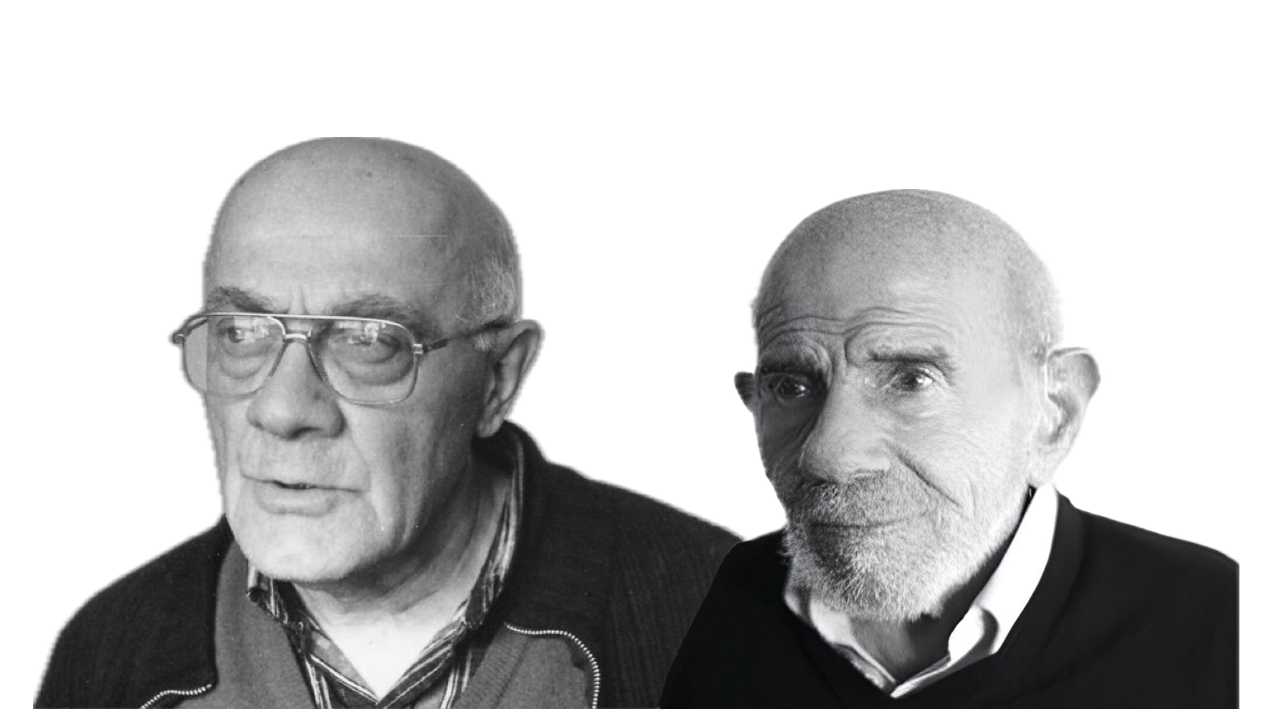
\includegraphics[width=\textwidth,trim=4 4 4 4,clip]{pictures/title.png}
    \vfill
\end{titlepage}

\tableofcontents

\chapter{История и философия науки как научная и учебная дисциплина}
\section{Философия науки, ее объект, предмет и структура. Роль философии в науке }   

\subsection{Философия науки, ее объект и предмет}

% Философия науки (ФН) – философская дисциплина, исследующая структуру научного знания, средство и 
% метода научного познания, а также способы обоснования и развития научного знания.

% В широком смысле, это философская дисциплина, занимающаяся осмыслением места и роли науки в отношении <<человек~—~мир>>.

% В узком смысле — деятельность ученых, посвященная философским и этическим проблемам развития науки.

% Объектом философии науки является наука как социальный и культурный феномен, а её предметом — познавательные структуры и методы, механизмы научного открытия, принципы объяснения и % обоснования научных знаний, а также этические аспекты науки.

Философия науки (ФН) --- философская дисциплина, исследующая структуру научного знания, средство и 
метода научного познания, а также способы обоснования и развития научного знания.

ФН как дисциплина появляется на рубеже 19-20 вв. В западной традиции принято 
использовать понятие эпистемология, но по содержанию это понятие уже, чем ФН, процесс познавательной 
деятельности в науке, ФН шире, структуру.

Объект ФН --- наука как исторически изменчивое единство её важнейших элементов (знание, техника, 
научные институты, типы научной деятельности, субъекты науки). Наука исторична, меняется вместе со 
сменой исторических эпох.
 
Предмет ФН --- наука, рассматриваемая через призму философии данной эпохи и общества. Точка анализа 
науки изменчива исторически, меняется наука и философия науки, который её исследует.

\subsection{Структура философии науки}

\subsubsection{Исследование науки как социокультурного феномена, как вида сознания и знания}

;-)

\subsubsection{Изучение философско-методологических оснований науки}

Онтологические представления о том, 
как устроен мир, гносеологические – методы достижения истинного знания, методологические 
знания -0 какой метод лежит в основе науки.
 
\subsubsection{Анализ проблемы возникновения науки и основных стадий ее развития
}
Существует два подхода к пониманию развития науки. Согласно концепции \textit{континуизма}, наука развивается поступательно и непрерывно, следуя эволюционному ходу. Концепция \textit{дисконтинуизма} утверждает, что развитие науки прерывается научными революциями, после которых она переходит на качественно новый этап с изменёнными фундаментальными представлениями.
    
\subsubsection{Изучение социокультурной динамики науки}

Иначе — определение движущих сил развития науки. Выделяются позиция \textit{экстернализма}, согласно которой основными движущими силами развития науки являются внешние факторы (например, социальный заказ, социальные ожидания от науки), а также позиция \textit{интернализма} - основными движущими силами развития науки являются внутренние факторы (интеллектуальные философские, собственно научные).
    
\subsubsection{Исследование философских проблем областей научного знания} 

Например, проблема жизни. Что такое жизнь с точки зрения различных научных дисциплин? Как эти разные понимания жизни объединяются? Есть ли у физики, биологии, химии, психологии нечто общее в понимании того, что такое жизнь? 

Или проблема происхождения Вселенной. Существовала ли она всегда, либо она появилась в какой-то момент?
        

	\subsection{Функции философии в науке} 

Долгое время обсуждалось, как отделить философию от науки и минимизировать её влияние, вплоть до полного устранения. Однако с конца XIX века, когда философия стала частью профессиональной подготовки ученых, возникла необходимость понять, какую роль она играет в научном образовании. 

Можно выделить несколько функций, которые философия выполняет в рамках научной деятельности.
\begin{itemize}
    \item \textit{Интегративная}. 
    Системное, целостное обобщение разнообразных форм познания, практики и культуры. Создание всеобщего и универсального знания.

    \item \textit{Критическая}. 
    Выяснение границ применимости получаемого человеком знания. Формирует критического сознания.  

    \item \textit{Мировоззренческая}. 
    Разработка определенных моделей реальности, сквозь призму которых ученый смотрит на предмет исследования (например, материализм, идеализм, дуализм)

    \item \textit{Гносеологическая}. 
    Исследование наиболее общих закономерностей познавательного процесса.

    \item \textit{Методологическая}. 
    Создание общенаучных методологических принципов. 
    Например, принцип инструментализма (Галилей) — для получения научного знания необходимо использовать приборы и измерительные инструменты.
    Либо принцип историзма — рассмотрение явления без отрыва от контекста его возникновения, протекания и привязки к определенной эпохе и обществу.
    
    \item \textit{Аксиологическая}. 
    Формирование определенных мировоззренческих и ценностных установок ученого. Это ответ на вопросы: <<зачем заниматься наукой?>>, <<что является в науке главной ценностью?>>, <<какую роль наука выполняет 
    в культуре и в обществе?>>, и т.п.

    \item \textit{Прогностическая}. 
    Разработка идей и представлений, значимость которых обнаруживается на будущих этапах развития науки. 
    Например, принцип атомизма — представление о том, что все твердые тела состоят из мельчайших элементов. Появился еще в античности, долгое время не был востребован в науке, но в 18 веке стал центральной опорой 
    всего корпуса химического знания. 
\end{itemize}
	
	\section {Проблема взаимосвязи философии и науки и основные концепции ее решения}

Еще в период античности возникает вопрос: <<как элементы научного знания взаимосвязаны и взаимодействуют с философией?>>. Рассмотрим концепции взаимосвязи философии и науки.

\subsubsection{Метафизическая концепция}

Появилась в античности усилиями Аристотеля.

Философия - это знание целого, а наука — это знание об отдельных областях действительности.
Философия — это некое состояние ума, которое позволяет рассуждать о предельных основаниях, о бытии, об истине и о ценности, а наука (или эпистема) — это знание, которое можно обосновать с помощью доказательства (например, математическое доказательство). 

Наука включается в рамки философии, так как наука является частным случаем рассуждения о всеобщих основаниях.
Аристотель приводит такое утверждение: все частные <<науки>> возникают из философии (н-р, геометрия, математика, астрономия, биология, география).

\subsubsection{Позитивистская концепция}

Возникла в XIX веке. Основоположник концепции — Огюст Конт. 

Наука — это особый вид познавательной деятельности, являющийся самодостаточным и обладающий приоритетом среди остальных видов познания. 
Это логический вывод из концепции развития общества Конта, где он выделяет три стадии: 
\begin{enumerate}
    \item \textit{теологическая}. Окружающий мир объясняется с точки зрения религиозных представлений (н-р, анимизм, тотемизм, фетишизм);
    \item \textit{метафизическая}. Окружающий мир объясняется с точки зрения философии (период: от античности до XIX века);
    \item \textit{позитивная} (научная). Окружающий мир объясняется с точки зрения науки.
Каждый раз, когда происходит смена этапа развития общества, предыдущий способ объяснения мира не исчезает, но он теряет свой приоритет.
\end{enumerate}

Концепция оказалась продуктивной для развития науки, так как позволила науке выработать собственный строгий методологический инструментарий, благодаря чему в 19-20 веке произошли громкие научные открытия. 
Однако позитивизму не удалось отделить философию от науки — ни в плане научного языка, ни в плане научной методологии, ни в плане мировоззрения. 

\subsubsection{Антиинтеракционизм}

Возник в начале 20 века на фоне Первой Мировой войны (Ж.-П. Сартр, К. Ясперс, Н.А. Бердяев). 

Основные проблемы общества — из-за науки, так как технический прогресс привел к глобальным социальным проблемам (мировая война, массовый голод, эпидемии).
Наука не способна исследовать подлинное бытие, что с точки зрения ряда философских направлений является внутренним миром человека 

\subsubsection{Диалектическая концепция}

Представители — Г. Гегель, Б.М. Кедров, В.С. Степин.

Философия и наука — это разные способы познания, но которые не могут существовать друг без друга. Философия изучает всеобщее, наука изучает частное. При этом философия без науки пуста, но наука без философии слепа.


\section {Наука как предмет прикладных исследований в ХХ веке в контексте научно-технической революции и развития <<большой науки>>}

\subsection{История исследований феномена науки.}

\subsubsection{XIX век. Дискуссия между Фрэнсисом Гальтоном и Альфонсом Декандолем}

Она касалась причин возникновения науки. Гальтон связывал развитие науки с расовыми особенностями, утверждая, что наука была создана исключительно белой расой. Декандоль, напротив, в своей книге «История науки и ученых за два века» (1873) на основе статистического анализа выделил 20 социальных факторов, определяющих развитие науки, таких как развитая система образования, доступ к материальным ресурсам, благоприятный климат и поддержка общественного мнения. Он доказал, что развитие науки зависит от социальных условий, а не от расы.

\subsection{«Большая» и «малая» науки. Основные тенденции развития науки в XX веке. Понятие научно-техничес-кой революции}

С точки зрения Дерека Прайса, основоположника современного прикладного исследования науки, в истории науки было несколько периодов:
\begin{enumerate}
    \item малая наука — разрозненные усилия отдельных людей по познанию окружающего мира (в античности, средневековье и в эпоху Возрождения);
    \item наука — в классическом понимании, возникшая в период нового времени (XVII век);
    \item большая наука (XX век) — характеризуется резким увеличением числа ученых, реализацией больших научных проектов и резким ростом научной информации.
\end{enumerate}
\textbf{Факторами формирования} большой науки являются:
\begin{itemize}
    \item Первая и Вторая мировые войны (высокий спрос на прикладные научные исследования);
    \item возникновение тесной связи науки и государства (глобальные и дорогостоящие научные проекты);
    \item рост роли науки в культуре общества.
\end{itemize}
К \textbf{особенностям большой науки} можно отнести:
\begin{itemize}
    \item резко возросшее число ученых (XVIII век~$\cong 10^3$, XX век~$\cong 10^6$);
    \item рост количества научной информации (в XX веке объем научной информации удваивается с периодом 10-15 лет);
    \item превращение науки в профессиональную деятельность;
    \item научно-техническая революция (в конце 40-х годов XX века);
    \item реализация больших научных проектов.
\end{itemize}

\textbf{Научно-техническая революция} — это коренное преобразование производительных сил общества на основе науки.

\subsection{Комплекс современных дисциплин, изучающих различные аспекты науки}

\subsubsection{Науковедение}

Основоположник — Джон Берналл («Социальная функция науки» — 1938 г.).

Задачей \textit{аналитического} направления науковедения является раскрытие закономерностей развития науки. 

\textit{Нормативное} науковедение занимается разработкой основ совершенствования организации научной деятельности. Нормативное науковедение стремится оптимизировать структуру науки для того, чтобы она работала более эффективно. 

\subsubsection{Социология науки}

Представители — Л. Флек и Р. Мертон.

С точки зрения Л. Флека задача социологии науки — это исследование интеллектуальных коллективов, изучение взаимодействия ученого (как индивида и личности) со своей социальной группой.

С точки зрения Роберта Мертона социология науки изучает универсальные нормы научной деятельности (объективизм, коллективизм и т.д.), или т.н. научный этос. 


\subsubsection{Наукометрия}

Основоположник — В.В. Налимов.

Задача наукометрии — измерить количественные результаты научной деятельности, эффективность как отдельного ученого, так и научного коллектива с целью дальнейшего принятия организационных решений в области науки.

\subsubsection{История науки}

История науки занимается проблемой возникновения и развития феномена науки. Можно выделить несколько уровней исторического исследования феномена науки:
\begin{itemize}
    \item наука в контекст развития общества (н-р, <<почему именно в Древней Греции возникает преднаучное знание?>>);
    \item наука как социокультурного феномена (н-р, история российской науки);
    \item история отдельных наук;
    \item история отдельного открытия, исследователя и т.п.
\end{itemize}

\subsubsection{Психология науки}
Изучает психологические факторы научной деятельности. Среди ее основных задач следующие: 
\begin{itemize}
    \item исследование психологических механизмов производства научных знаний в условиях индивидуальной и коллективной деятельности;
    \item разработка проблем психологической подготовки научных кадров, диагностики и формирования соответственных личностных качеств и установок;
    \item разработка проблем возрастной динамики творчества;
    \item анализ психологических аспектов научных коммуникаций, восприятия и оценки новых идей;
    \item анализ психологических аспектов автоматизации и компьютеризации исследований.
\end{itemize}
По большому счету психология науки занимается психологическим аспектом труда ученых. 

\subsubsection{Hормативно-правовое регулирование научной деятельности}

До конца Второй мировой войны, до так называемого Нюрнбергского трибунала практически не было практики нормативно-правового регулирования труда ученых. 

\texttt{Нюрнбергский кодекс}. Кодекс включает в себя несколько принципов, из которых, например, <<Добровольное согласие испытуемого на медицинский эксперимент>>; <<Интересы индивида преобладают над интересами научного сообщества>>.

\texttt{Хельсинская декларация Всемирной медицинской организации (1964 г.)}. 
Представляет собой набор этических принципов для медицинского сообщества, касающихся экспериментов на людях. Введено разделение на исследования:
\begin{itemize}
    \item c лечебной целью — которые направлены на разработку новых методов лечения или применяются в ситуациях, когда другие способы помочь пациенту невозможны, а его состояние угрожающее.
    \item с теоретической целью — которые изучают особенности работы организма, например, реакции на экстремальные условия (перегрузки, переохлаждение, отсутствие сна), без непосредственного лечебного значения.
\end{itemize}

\texttt{Конвенции о правах человека и биомедицине}. Сформулирован принцип необходимости этических комитетов, осуществляющих независимую экспертизу обоснованности необходимости проведения эксперимента.

\texttt{Декларация о геноме человека и правах человека (ЮНЕСКО)}. В декларации постулируется, что геном человека – основа изначальной общности всех представителей человеческого рода, и он не должен служить источником извлечения доходов. Все геномные исследования должны быть тщательно выверены, их обоснованность не должна вызывать никаких сомнений, и каждое национальное государство обладает своим суверенитетом в деле разрешения или запрещения геномных исследований. 

Наиболее явным образом нормативно-правовое регулирование научной деятельности осуществляется для исследований, направленных на изучение человека (медицинские, физиологические и пр.). Можно ожидать, что со временем начнет регулироваться и научная деятельность как таковая, поскольку современные исследования могут иметь последствия, которые необходимо учитывать в глобальном планировании развития экономики и общества.

\chapter{Многообразие научного знания и его структура}
\section{Различные типы знания. Специфика научного знания и его критерии}  

\subsection{Сущность знания и познания}

\subsubsection{Понятие знания}
 
Знание ~---~ это \textit{проверенный практикой} результат познавательной деятельности, 
форма социальной и индивидуальной памяти. Знание выступает в виде усвоенных понятий, законов,
принципов и так далее.  

Знание можно разделить на две большие группы: 
\begin{itemize}
    \item \textit{знание-умение} (практическое знание, «знание как»). Имеет специфическую проверку (н-р, можно уметь или не уметь кататься на велосипеде, но нельзя
кататься на велосипеде истинно или ложно);
    \item \textit{знание-информация} (<<знание что>>) --- о наличии у предметов каких-то свойств, знание о закономерностях, знание о последовательности действий в той или иной ситуации. Для него характерна проверка на истинность.  
\end{itemize}


Любое знание нуждается в
объективации. В продуктах труда, в технологиях, в социальных институтах, в
произведениях искусства, в текстах. Даже когда мы говорим об индивидуальном
знании, то, которое содержится только в нашей памяти, оно объективируется там в
понятиях, в образах, в воспоминаниях и в других формах.  После своей
объективации знание может быть передано другому человеку.  

Субъект знает некий предмет, если соблюдаются следующие условия:
\begin{itemize}
    \item условие истинности предмета;
    \item условие убежденности/приемлемости;
    \item условие обоснованности.
\end{itemize}


\subsubsection{Понятие познания}

\textit{Познавательная
деятельность} --- это сознательная деятельность субъекта, направленная на
приобретение информации об объектах и явлениях реальной действительности. Это
единство чувственного восприятия, теоретического мышления и практической
деятельности.  

В результате познания формируется
познавательный образ --- образ, возникающий в сознании при непосредственном или
опосредованном взаимодействии субъекта с объектом.  

Познавательные образы делятся на: 

\begin{itemize}
    \item чувственные образы:
    \begin{itemize}
        \item элементарные (ощущение, восприятие и представление);
        \item синтетические (чувственные образы, стереотипы, художественные образы, модельные представления);
    \end{itemize}
    \item рациональные образы (теоретическое восприятие особенностей класса предметов 
через систему всеобщих и необходимых свойств этого класса, выраженных
в понятии):
    \begin{itemize}
        \item элементарные (понятия, термины);
        \item синтетические (совокупность понятий, связанных 
единым смыслом или единой политикой их применения в теории или в гипотезе).
    \end{itemize}
\end{itemize}

\subsection{Особенности научного знания} 

\subsubsection{Системность} 

Наука --- это иерархически организованная система знаний, которая делится на отдельные дисциплины. Изменение значимого элемента в этой системе приводит к постепенному пересмотру всей структуры научного знания (например, переход от физики Ньютона к физике Эйнштейна).

\subsubsection{Объективность} 

Наука стремится изучать предметы и явления так, как они существуют в объективной
реальности. Поэтому знание можно проверять на практике, в эксперименте, в
наблюдении и другими способами. 

\subsubsection{Культурно-историческая обусловленность}

Наука зависит от периода и общества, в котором она развивается. Общие характеристики науки существуют, но они абстрактны. Наука исторически меняется, и современная её версия сильно отличается от науки прошедших эпох, несмотря на общую основу.

\subsubsection{Всеобщность}

Научное знание изучает общие законы и свойства предметов, стремясь формулировать универсальные законы, применимые в любой точке Вселенной. (Хотя и существует гипотеза о возможных исключениях во Вселенной, она остается неподтвержденной.)

\subsubsection{Необходимость}

В научном знании фиксируются системообразующие стороны явлений. 

\subsubsection{Дисциплинарная принадлежность}

Научное знание можно распределить по различным дисциплинам, что представляет собой горизонтальную структуру. Вертикальная структура связана с иерархией уровней. Междисциплинарное знание возникает на стыке дисциплин, но часто приводит к созданию новых дисциплин, таких как физическая химия или эволюционная психология.

\subsubsection{Подтверждение научным сообществом}

В XVII-XVIII вв., когда институт науки только формировался, распространенной практикой было приглашение ученых или уважаемых людей для демонстрации экспериментов, чтобы подтвердить результаты. Если эксперимент не удавался, ученый мог быть подвергнут остракизму. Сегодня существуют институциональные механизмы подтверждения научных результатов, такие как рецензирование и редактирование статей, а также защита диссертаций, которые обеспечивают коллективное признание научных достижений.

\subsection{Научные конструкты и требования к ним}

Объект
исследования, который чаще всего наука изучает, является не самим объектом, а
является конструктом.
\textit{Научный конструкт} --- это умозрительное построение, вводимое гипотетически
и создаваемое по правилам логики. 

К ним выдвигаются следующие требования:
\begin{itemize}
    \item возможность логических операций над конструктами как языковыми выражениями;
    \item множественность связей между конструктами в рамках некоего целого;
    \item устойчивость конструктов (то есть постоянство значений в различных контекстах);
    \item экстраполируемость конструктов (то есть возможности их максимально широкого использования помимо породивших их ситуаций);
    \item согласованность выражений конструктов с установленными закономерностями;
    \item простота конструктов.
\end{itemize}

\subsection{Сравнительная характеристика
научного и обыденного знания}

\begin{longtable}{|>{\raggedright\arraybackslash}p{7cm}|>{\raggedright\arraybackslash}p{7cm}|}
\hline
\textbf{Обыденное знание} & \textbf{Научное знание} \\
\hline
\endfirsthead

\hline
\textbf{Обыденное знание} & \textbf{Научное знание} \\
\hline
\endhead

непрофессиональное, неспециализированное жизненно-практическое, повседневное знание & Продукт специализированной, профессиональной формы человеческой деятельности \\
\hline
не имеет строгого концептуального, логического, системного оформления. & носит теоретический, концептуальный характер; отличается системной организацией \\
\hline
не требует для своего усвоения специального обучения и подготовки & требуется специальное обучение для овладения им\\
\hline
констатация явлений, связей и отношений & ориентировано на поиск закономерностей \\
\hline
может иметь субъективный характер & в идеале должно быть объективным, доказательным, точным \\
\hline
предмет всегда нагляден и доступен восприятию & включает в себя системы абстрактных объектов \\
\hline
дается преимущественно как типичное, понимаемое по аналогии & имеет творческий характер\\
\hline
осуществляется познание единичных ситуаций и явлений & носит универсальный характер \\
\hline
решает конкретные, сиюминутные жизненные проблемы & выходит за рамки практической заинтересованности \\
\hline
использует для фиксации знания устную разговорную традицию &  использует письменную традицию \\
\hline
\end{longtable}


Проблема демаркации научного и обыденного знания остаётся нерешённой, потому что обыденное знание часто предшествует научному. Наука возникает на базе первичных представлений о свойствах объектов, с которыми человек взаимодействует в повседневности. Кроме того, наука использует естественный язык, схожий с тем, который применяется в обыденном знании, хотя стремится к большей формализации. 

В истории были попытки создать строго формализованный научный язык, свободный от недостатков естественного, но полностью это не удалось. Исключение составляет, возможно, математика, которая может быть рассмотрена как формализованный язык. Научный язык и язык обыденного знания связаны через общие понятия и вложенные в них смыслы.



\section{Основные классы научного знания и их дисциплинарная организация} 

\subsection{Проблема классификации науки}

Научное знание может быть классифицировано на определенные
элементы. Проблема классификации наук заключается в том, что в
результате этой классификации необходимо раскрыть взаимосвязи между элементами
науки и выработать представление о ее некой целостной структуре. 

В истории философии были неоднократные попытки классифицировать научное знание. 
Рассмотрим некоторые из них.

\subsubsection{Классификация Аристотеля (384-322 гг. до н.э.)}

Аристотель делил знание на: 

\begin{itemize}
    \item \textit{теоретическое}, где познавательная деятельность ведется ради самого познания. И философия, и наука относятся к теоретическому знанию, занимаясь познаванием из
    отстраненной позиции, пытаясь созерцать явления во всей полноте. 
    \item \textit{практическое}, где познание ведется для выработки идей для поведения человека; К практическому знанию относятся те отрасли, которые
    вырабатывают определенные принципы поведения человека в жизни (повседневной, политической, и т.д.). Например, этика и политика.
    \item \textit{творческое}, где познание осуществляется для достижения чего-либо
    прекрасного. К творческому знанию относятся виды деятельности, направленные на
получение чего-то прекрасного. Например, риторика, поэтика, живопись.
\end{itemize}

В основании классификации положен принцип цели
познавательной деятельности. Данная классификация не приближает к
пониманию специфики науки, определенного класса знания. 

\subsubsection{Классификация Фрэнсиса Бэкона (1561-1626 гг.)}

Науки делятся на: 
\begin{itemize}
    \item \textit{исторические} --- описание фактов (как гражданских, так и естественных);
    \item \textit{теоретические}, или философия в широком смысле слова;
    \item \textit{поэтические} --- литература, искусство, поэзия. 
\end{itemize}

В основании классификации Бекона лежит принцип опоры на определенные
интеллектуальные способности: память, разум или воображение. 
При выборе интеллектуальной способности возникает
класс научного знания. Однако внутри класса трудно провести дальнейшую
спецификацию. 

\subsubsection{Классификация Георга Гегеля (1770-1831 гг.)}

Исходя из своей системы диалектики, он делит знания на три раздела: 
\begin{itemize}
    \item \textit{логика}: учение о бытии, учение о сущности и учение о понятии;
    \item \textit{философия природы}: механика, физика и органическая физика;  
    \item \textit{философия духа}: изучение субъективного духа (человека), объективного духа (общества) и абсолютного духа (Бога). 
\end{itemize}

Система является стройной, и внутреннее деление на дисциплины близко к современной классификации. 

\subsubsection{Классификация Огюста Конта (1798-1857 гг.)}

Им предложена следующая классификация:

\begin{itemize}
    \item математика (вкл. механику);
    \item астрономия;
    \item физика;
    \item химия;
    \item биология;
    \item социология.
\end{itemize}
При движении от математики к социологии
увеличивается сложность предмета исследования: геометрические фигуры, числа, их
взаимодействие наиболее простой предмет исследования, а социальные процессы ---
наиболее сложные. 

В обратную сторону происходит
увеличение абстрактности предмета: у социологии предельно конкретный предмет
исследования, у математики --- предельно абстрактный. 

Предметы исследования в данной классификации достаточно изолированы друг от друга. 

\subsubsection {Классификация Фридриха Энгельса (1820-1895 гг.)} 

\begin{itemize}
    \item механика;
    \item физика;
    \item химия; 
    \item биология; 
    \item социология. 
\end{itemize}

Предметы не изолированы, а
дисциплины означают диалектический переход от одной формы движения материи к другой.
Т.о., социальная форма движения
материи включает в себя остальные формы движения материи, но ими
не определяется по своей природе. 


\subsubsection{Классификация В.И. Вернадского}

Вернадский разделял науки на две категории:
\begin{itemize}
    \item науки, законы которых охватывают всю реальность;
    \item науки, законы которых свойственны только Земле.
\end{itemize}

Эта классификация имеет практическую ценность в рамках концепции Вернадского о развитии планеты и общества. Для Земли характерны уникальные явления, такие как жизнь и разумный человек, которые не найдены в других частях Вселенной. Поэтому науки, изучающие человека и общество, являются уникальными для Земли. Напротив, такие науки, как физика и химия, охватывают всю реальность. 

\subsubsection{Современная классификация наук} 

В современности деление происходит по трем аспектам: предмет исследования, особенности методологии и критерии научности в данной отрасли.
\begin{itemize}
    \item математические науки;
    \item естествознание;
    \item гуманитарные науки;
    \item социальные науки;
    \item технические науки.
\end{itemize}
 
\subsection{Фундаментальное и прикладное научное знание} 

Разделение наук на фундаментальные и прикладные --- еще один вариант классификации, который широко используется, в том числе для повседневного описания науки. 

\subsubsection{Фундаментальная наука}

Это область научного познания, включающая теоретические и экспериментальные исследования
основополагающих явлений. 

Фундаментальная наука характеризуется концептуальной универсальностью и всеобщностью во времени и пространстве. Ее выводы применимы ко всем системам и условиям в любой точке Вселенной и касаются основополагающих явлений, таких как строение материи, энергия, фундаментальные взаимодействия и эволюция Вселенной. 

\subsubsection{Прикладная наука}  

Направлена на интеллектуальное обеспечение инновационного процесса, как основы развития современной цивилизации. Прикладная наука обеспечивает конкурентное преимущество.

Прикладные научные исследования начали развиваться в 19 веке благодаря деятельности Юлиуса фон Либиха, который систематически использовал науку в интересах промышленности, начиная с химической отрасли. 

\subsection{Дисциплинарная структура науки}

Научная дисциплина --- это форма систематизации научного знания.
Она формируется на основе общности объекта исследования, методов, идеалов и норм исследований.  

Для появления научной дисциплины важно не только осознание общности
элементов, но и появление институциональных форм существования научной
дисциплины. 
Кроме этого, в дисциплинарной структуре науки постоянно происходит интеграция и
дифференциация научных дисциплин. 
Дифференциация подразумевает собой появление дисциплин со все более узким предметом
исследования. 
Интеграция, наоборот, означает то, что предмет исследования
расширяется.


\section{Уровни научного познания и соответствующие им методы и формы знания}
 
\subsection{Эмпирический уровень научного познания}

В результате непосредственного или опосредованного контакта с
предметом исследования ученые получают знания об определенных событиях и явлениях. 

\subsubsection{Формы эмпирического знания}

\textbf{Научный факт} --- это форма эмпирического научного знания, в которой фиксируется
некоторое конкретное явление или событие. 
Чтобы факт мог называться научным, необходимо соблюсти следующие требования:
\begin{itemize}
    \item отношение к определенной предметной области науки; 
    \item содержательное описание процедуры и  обстоятельств фиксации события;
    \item усредненность результатов наблюдений и измерений; 
    \item воспроизводимость в научной деятельности  других  исследователей;  
    \item соотношение  с  некоторой  совокупностью, системой родственных или схожих фактов;
    \item теоретическая нагруженность (понятия, с помощью
    которых факт формулируется, соотносится с определенной научной теорией, и в
    рамках этой теории обладают определенным смыслом).
\end{itemize}

Научный факт имеет определенную структуру, состоящую из трех
компонентов:
\begin{itemize}
    \item \textit{перцептивный} компонент --- это чувственный образ, который возникает в
    результате восприятия явления;
    \item \textit{материально-практический} компонент --- это
    совокупность приборов, инструментов и действий с ними, используемых для
    установления факта;
    \item \textit{лингвистический} компонент --- это высказывание, формулирующее факт.
\end{itemize}


\textbf{Эмпирическое обобщение} --- это форма знания, которая фиксирует в
себе некую внешне проявляющуюся причинно-следственную связь. Например, если мы 10 раз уронили бутерброд с маслом, и он каждый раз падал маслом вниз, мы можем сформулировать эмпирическое обобщение, что бутерброды с маслом, вероятно, будут падать маслом вниз. Причины этого явления нам пока неизвестны, но мы зафиксировали внешнее проявление причинно-следственной связи: уроненный бутерброд всегда падал маслом вниз.

\subsubsection{Методы эмпирического знания}

Среди эмпирических методов выделяют наблюдение, эксперимент, сравнение, описание и измерение.

\textit{Эксперимент} --- это метод эмпирического научного
исследования, который подразумевает активное и целенаправленное вмешательство в
протекание изучаемого процесса, в том числе в специально созданных и
контролируемых условиях. 

Научное \textit{наблюдение} предполагает фиксацию некого внешнего изменения того или иного процесса. 

\subsection{Теоретический уровень научного познания}

Теоретическое познание описывает идеальные объекты,
которые, в отличие от реальных объектов, характеризуются конечным числом свойств. 

\subsubsection{Формы эмпирического знания}

К ним относятся проблема, гипотеза, закон и теория.

\texttt{Научная теория} --- это форма теоретического научного знания, содержащая целостное
отображение закономерных и существенных связей определенной области действительности.

Научная теория представляет собой высокий уровень организации научного знания, \textit{включая гипотезы, концепции, закономерности и законы}, которые составляют теорию. Теория --- это квинтэссенция теоретического знания, объясняющая явления в широкой предметной области. 

Например, теория всемирного тяготения не ограничивается падением яблока, а охватывает общие принципы взаимодействия материи. Теория эволюции описывает общий процесс эволюции, а не изменения отдельных видов животных.

Компонентами научной теории являются: 
\begin{itemize}
    \item исходные основания --- фундаментальные понятия, принципы, законы, аксиомы,
    которые являются отправной точкой теоретического исследования объекта;
    \item идеализированный объект --- модель существенных свойств и связи
    изучаемых предметов;
    \item логика теории --- совокупность определенных правил и способов доказательства;
    \item философские установки, социокультурные и ценностные факторы (н-р, элементы картины мира самого ученого);
    \item совокупность утверждений, выводимых из этой теории в качестве следствий.
\end{itemize}

\subsubsection{Методы теоретического знания}

Среди теоретических методов выделяют формализацию, аксиоматический подход, гипотетико-дедуктивный метод, обобщение и идеализацию. 

\textit{Гипотетико-дедуктивный метод} заключается в создании системы дедуктивно связанных между
собой гипотез, из которых выводится утверждение о возможных эмпирических фактах. Далее, в эксперименте или в наблюдении отыскиваются спрогнозированные факты. Если они
обнаружены, то гипотеза косвенно подтверждается.  

\subsection{Метатеоретический уровень научного познания}

На метатеоретическом уровне научного познания вырабатываются идеи и принципы, 
с помощью которых происходит обоснование представлений научной картины мира. 
Они служат одним из условий включения научных знаний в культуру соответствующей 
исторической эпохи. 

\subsubsection{Формы метатеоретического знания}

К ним относятся научная картина мира, научная парадигма, общенаучные принципы и философские основания науки.

\texttt{Философские основания науки} --- это
система философских идей, которые используются для обоснования различных
аспектов научной деятельности. Рассмотрим некоторые основания науки:

\begin{itemize}
    \item \textit{онтологические} --- принятые в данной науке представления о строении окружающего мира;
    \item \textit{гносеологические} --- содержат представление о критериях истинности знания;
    \item \textit{логические} --- содержат представление о той логике, которой нужно оперировать для доказательства;
    \item \textit{аксиологические} --- содержат представление о главных ценностях науки (н-р, получение нового знания, пользы для человека, и т.п.);
    \item {методологические} --- представление о том, с помощью какой методологии мы можем получать истинное научное знание (эксперимент, математическое моделирование, и т.п.).
\end{itemize}

\subsubsection{Методы метатеоретического знания}

К ним относятся методологическая рефлексия и философские методы.

\textit{Философские методы} --- методы познания, которые являются сугубо философскими. 
Например, диалектический метод --- метод рассмотрения
развивающихся явлений через диалектическую логику единства и борьбы
противоположностей, перехода количества в качество и отрицания отрицания.

\textit{Методологическая рефлексия} --- это исследование оснований собственной научной
деятельности с точки зрения общих принципов познавательного процесса. 


\chapter{Социально-коммуникативные аспекты науки}
\section{Коммуникативные аспекты науки} 

\subsection{Понятие коммуникации, статус коммуникации в рамках научной деятельности}

\subsubsection{Понятие коммуникации}

% Например, в английском common, community, communication, однокоренные
% слова, которые означают общий, сообщество, общество и связь, общение, сообщение
% соответственно. 

% Слово коммуникация имеет латинское происхождение. От communico
% делаю общим. 

% Благодаря коммуникации человек развивает мыслительные способности
% объединять свои усилия с другими, чтобы строить цивилизацию. Хотя анатомически
% похожие на нас люди были уже 200 тысяч лет назад. Они обрели культуру, начали
% одеваться, хранить мертвых, оставлять рисунки и так далее. Только 50 тысяч лет
% назад, когда придумали язык и начали общаться. Ну а письменность появилась всего
% 6 тысяч лет назад. Так что это новость в масштабах Вселенной. Ну и огромный наш
% эволюционный скачок. 

Среди определений человеческой коммуникации наиболее
распространены такие варианты, как обмен информацией и общение людей. 

В широком смысле, коммуникация представляет собой связь, взаимодействие,
предполагающее положительное взаимно связывающим некими потоками отношение (???).

Основные отличительные черты человеческой коммуникации:
\begin{itemize}
    \item процесс, который предполагает двух и более участников (при общении с собой --- противопоставление самому себе);
    \item передача опыта, смысла, эмоций, информации и т.д.;
    \item восприятие и интерпретация;
    \item длящийся во времени и требующий времени (для осмысления) процесс;
    \item совместность, осуществление связи между;
    людьми, обычно с целью некого взаимного положительного эффекта, предполагающего
    взаимное духовное развитие, обогащение, понимание.
\end{itemize}

\subsubsection{Статус коммуникации в рамках научной деятельности}

В научной среде коммуникация не должна претендовать на основное место в процессе научной работы. Коммуникация и коллективная работа важны наряду с индивидуальной
деятельностью, только в рамках которой возможно творчество. 

Несомненно, обмен
знаниями и совместное планирование исследования, постановка проблемы, поиск
методов ее решения, обсуждение полученных результатов и так далее, крайне важны
для научно-исследовательской работы.

Творчество, производство нового знания — ядро собственно научной деятельности.
Без творческой составляющей, просто из общения как обмена готовыми мнениями научное знание не
могло бы родиться. 

Согласно исследованиям французских мыслителей
XX века Жиля Делёза и Феликса Гваттари, творчество всегда единично. 

Это означает, что
коммуникация как обмен мнениями может лишь способствовать творчеству, вдохновить
человека, обратить внимание одного на то, что более ясно видится другому с его
точки зрения, но не в силах заменить собой творческий элемент научной
деятельности. 

Макс Вебер утверждал, что помимо коммуникации и творчества,
значимой оказывается и повседневная рутинная работа, не в меньшей
степени обеспечивающая и подготавливающая научное открытие.

Таким образом, коммуникация в научной сфере имеет
достаточно важное значение, однако скорее выполняет вспомогательную и
интегративную функцию, чем играет единственную ведущую роль.


\subsection{Формы и способы коммуникации в научной среде}

Благодаря достижениям техники можно
выделить также и широкий спектр инновационных
возможностей и средств для осуществления профессионального общения.

\begin{table}[h!]
\centering
\begin{tabular}{|p{6cm}|p{6cm}|}
\hline
\textbf{Традиционные} & \textbf{Инновационные} \\ \hline
Личная беседа & Интернет-технологии \\ \hline
Письма & Аудио- и видеоконференцсвязь \\ \hline
Научные публикации & Дистанционные технологии подачи и рецензирования публикаций \\ \hline
Конференции, лекции, теоретические доклады, совещания, съезды & Онлайн-встречи, вебинары \\ \hline
Стажировки, повышение квалификации, совместные праздничные мероприятия & Интерактивные игровые формы: тренинги, модели, неформальные корпоративы \\ \hline
\end{tabular}

\label{table:traditional_vs_innovative}
\end{table}

Личное общение дает больше опыта коммуникации и осуществления
научной деятельности, поскольку при этом участвует несколько каналов восприятия, 
есть возможность физического воспроизведения.

Майкл Полани поднимает важную тему личностного или неявного
знания. Знания обретаются не только в ходе устной или письменной коммуникации.
Ряд знаний, умений,
навыков для профессиональной деятельности обретается лишь в процессе регулярной
практической деятельности, зачастую оседая на бессознательном, интуитивном уровне.

Обычную коммуникацию в целом подразделяют на:
\begin{itemize}
    \item вербальную
        \begin{itemize}
            \item устную: дискуссии, сообщения, участие в конференциях и т.п.;
            \item письменную: статьи, отчеты, книги и т.п;
        \end{itemize}
    \item невербальную: мимика, жесты, взгляд, интонация, поза, темп и тембр речи.
\end{itemize}
Указанные формы выражения играют роль в рамках профессиональной коммуникации, поскольку выражения воспринимаются по-разному в зависимости от сложности конструкций, эмоциональной загруженности,
невербального оформления и соблюдения вежливости.


\subsection{Специфика научного языка}

Для научного языка характерны \textit{термины} (15-20\% научной лексики). Это слова или словосочетания, обозначающие понятия в специальной
области знаний или деятельности, которые стремятся к однозначности и не выражают
экспрессии. Важно, что у терминов есть референт в реальности. 

Большую часть научной лексики (30-40\%) составляют: \textit{абстрактная лексика}
\textit{специальные фразеологизмы}, \textit{клише и стандартные обороты}.

Для научных текстов свойственен академический стиль, имеющий следующие особенности:
\begin{itemize}
    \item логичность, непротиворечивость выражений;
    \item высокий регистр (исключение расхожих фраз, оборотов обыденного языка);
    \item четкость, ясность, умеренная простота конструкций;
    \item точность выражений (отсутствие двузначности, размытых и
    пустых формулировок, полное отражение всей фактической информации);
    \item безличные конструкции (употребление научного <<мы>>);
    \item научная лексика;
    \item аргументированность (доказательность и иллюстративность сформулированных
    положений).
\end{itemize}
Важно уметь отличать его от смежных стилей, соблюдая баланс в рамках официальной научной коммуникации. 

Нельзя также не сказать хотя бы в двух словах о нормах
научной коммуникации, которые  Часть этих моментов мы
рассмотрим подробнее в третьем вопросе сегодняшней темы, потому что они больше
относятся к этическим аспектам. 

\subsection{Нормы научной коммуникации}

Помимо очевидного соблюдения \textit{вежливости},
\textit{непредвзятости} и \textit{аргументированной критики}, к нормам научной коммуникации относятся к культура
цитирования и ответственность за самостоятельность получения и
представление результатов научной деятельности.

\subsubsection{Культура цитирования}

В рамках академического стиля действует следующая культура цитирования: 
\begin{itemize}
    \item принято ссылаться в основном на научные статьи и монографии (до 80\% источников цитирования);
    \item возбраняется ссылаться на неавторитетные и недостоверные источники;
    \item недопустимость плагиата.
\end{itemize}

Генеральная цель науки --- создание нового знания. 
Поскольку новое научное знание  как правило основано на уже созданных представлениях, необходимо соблюдать баланс между опорой на авторитетные источники и творческим элементом собственного исследования. 

\subsubsection{Самостоятельность получения и представление результатов}

% Сравним человека и большие языковые модели.

% Оно
% предполагает, в отличие от животных, прежде всего, рефлексивность в постановку
% вопросов и выход на уровень смысла, то есть осмысление, понимание. Также
% отмечают высокую развитость воображения и речи, когнитивных и коммуникативных
% способностей. 

% При этом интересно, что люди не рождаются с человеческой системой
% восприятия, не владеют языком и не умеют сразу мыслить. Собственно, человеческое
% именно формируется. Изначально у нас есть так называемая лепетная речь. Это
% слоговая непонятная речь детей, которой мы все с двух-трех месяцев начали
% пользоваться. 
% Также в нас заложены потребности выражать свое самоощущение в
% связи с происходящим вокруг и играть, примеривая на себя различные роли.
% Благодаря этим естественным предпосылкам в процессе взросления в среде
% человеческого общения ребенок проходит два фундаментальных кризиса. 

% Появление самосознания и развитие совести. Собственно, умение посмотреть на себя со
% стороны, отделяя я от мира, и внутренний диалог, учитывающий самостоятельность
% других, в горизонте максимально возможного, являются уникальными онтологическими
% особенностями человека, на которых и строится вся специфика его бытия по
% сравнению с другими существами. Развитие мышления и языковые способности
% неразрывно связаны. Переработка изначально лепетной речи в классифицирующие и
% маркирующие вещи события взрослый язык, помогает осваивать абстрактные формы,
% теоретические и оценочные инструменты, логическое, критическое и рефлексивное
% мышление. Безусловно, к творческому, исследующему и преобразующему отношению к
% миру у ребенка есть природная тяга. Однако в процессе взросления они получают
% огромный стимул к совершенствованию именно благодаря развитию речи и
% взаимодействию с другими. И человеческий язык не просто средство передачи
% информации, это многомерная и на большую долю иррациональная система. К тому же
% буквально среда нашего обитания, которая с одной стороны задает схему мышления,
% а с другой открывает возможности понимания смысла различных интерпретаций. Так
% что смоделировать все естество языка через логические операции вряд ли
% получится. На самом деле, задолго до распространения современных генеративных
% нейросетей в дискуссиях о таких мысленных экспериментах, как «Китайская
% комната», «Философские зомби», «Мозг в колбе» и так далее, Джон Сёрль, Сол
% Крипке, Дэвид Чалмерс, Дэниел Дэннет, Ник Бостром и другие аналитические
% философы показали, что антологически машинная речь «речь» может представлять
% собой лишь более или менее удачную имитацию типичного, за которой не стоит опыт,
% понимание, подлинное творчество и здравый смысл. Об этом, опять же, ребят, у нас
% будет еще разговор на последних темах, так что не пугайтесь, что я вам тут
% каких-то имен наговорила, мы позже с ними познакомимся. Но что касается так
% называемых больших языковых моделей, они организованы по принципу токенизации,
% надрабления на морфологические составляющие и комбинирования слов естественного
% языка. Обучение нейросетей для генерации текстов предполагает обработку системы
% огромного массива статей в Википедии, художественной литературы, новостных лент
% и других подобных ресурсов. Например, в обучении ChatGPT3 было включено 600
% гигабайт таких текстов, опубликованных в интернете до 2020 года. Из этих текстов
% выявляются закономерности совместного слова употребления, collocations и
% окончаний с присвоением более высоких коэффициентов в более распространенном
% конструкции. Соответственно, ответ на запрос пользователя, в ответ на запрос
% пользователя, выученная таким образом нейросеть, будет выдавать стереотипные
% фразы общими словами. Искусственно-интеллектуальные системы не понимают смысл ни
% запросов, ни своих ответов, ни той информации, на которой их обучили, ни того
% контекста, в котором ведется поиск. Поэтому актуализируются проблемы
% достоверности выдуваемых сведений, этичности содержания, логичности и
% соответствия здравому смыслу. То есть в отсутствии реального, критического,
% рефлексивного мышления, ответы генеративных нейросетей могут противоречить сами
% себе, быть предвзятыми, предоставлять вымышленные или несоответствующие
% действительности данные. К примеру, в ответ на вопрос, сколько минут следует
% варить 3 яйца, если 5 яиц варятся 10 минут, система выдаст 6 минут, что будет
% ошибкой здравого смысла. Или, к примеру, чат GPT считает, что у лошади 8 ног.
% Две правые, две левые, две передние, две задние. Я недавно спрашивала, Яндекс
% Алиса, например, полагает, что в ноябре только один вторник. Ну, то есть
% понятно, какие проблемы с ними возникают. Таким образом, говоря об
% онтологическом статусе, подчеркнем, что нейронная сеть это математическая
% модель, построенная на перцептронах, которые состоят из трех видов элементов.
% Принимающих сигнал, анализирующих его и выдающих реакцию. То есть какой-то
% ответ. Собственно, почему говорят о ненадежности результатов работы нейросетей и
% о том, что их сложно проверить, что они работают как черный ящик. В многослойных
% системах огромное количество таких перцептронов и не обязательно элементарных.
% На каждом из них, из этих миллиардов элементов, в каждом слое выполняется
% настолько много операций, что поиск узла, в котором, например, произошла ошибка,
% вручную просто нецелесообразен с точки зрения затрат времени и ресурсов. Обычно
% в случаях, когда нейросеть плохо обучилась, разработчики отправляют ее на
% переобучение, корректируя выбор, критерии и так далее. Но, естественно, любая
% выборка конечна и не сможет вместить в себя всю полноту реальности, с которой
% этой системе затем придется иметь дело. У нее нет воображения, поэтому она сама
% не сможет ничего оценивать. Она просто производит операции с блоками информации,
% у нее отсутствует выход в пространство абстрактных форм. Так, несмотря на
% некоторые биологические аналогии с работой нервных клеток, нейросети не являются
% живыми, это лишь инструмент работы с большими данными, пусть и сложный по своей
% архитектуре, и ресурсоемкий в плане воплощения в железе. У ныне распространенных
% искусственных систем отсутствует такая базовая характеристика всего
% одушевленного, как наличие воли. То есть нейросеть ничего не делает сама. За ее
% функционирование и использование могут отвечать только люди, разработчики,
% собственники и пользователи. Таким образом, применение генеративных нейросетей
% оправдано, к примеру, в случаях оптимизации рутинной работы, то есть
% автоматизации каких-то шаблонных действий или индуктивного обобщения. Но нужно
% ограничивать или осознанно контролировать их использование в случаях принятия
% экзистенциальных и этических решений, поскольку нейросети не способны осмыслять.
% И создание уникального творческого продукта, которым, например, является научная
% статья. 
Помимо проблемы плагиата, этот вопрос можно рассмотреть в контексте появившихся недавно нейросетей. Выделим следующие принципы использования нейросетей в научной деятельности и коммуникации:
\begin{itemize}
    \item недопустимо применение для обмана, оскорбления, подлога или искажения данных;
    \item недопустимо использовать при требовании самостоятельной работы;
    \item недопустимо применение в области принятия этических и экзистенциальных решений;
    \item декларировать использование, указывать объемы и аспекты применения.
\end{itemize}

\subsection{Коммуникация в сфере науки как ценность}

Наряду с ценностями самого научного знания (истинность, рациональность, общедоступность и др.), коммуникация в научной среде сама обладает огромной ценностью, поскольку:
\begin{itemize}
    \item является живой средой формирования и функционирования научного знания
    (научное знание выражается в языке, распространяется в среде);
    \item позволяет делиться опытом (обсуждение обогащает пониманием специфики исследования, позволяет учиться на чужих ошибках, подчеркнуть позитивный опыт);
    \item дает возможность рассмотреть проблему с различных точек зрения;
    \item высвечивает новые перспективы и вопросы;
    \item побуждает участников точно и ясно формулировать свои идеи.
\end{itemize}
Важно осуществлять коммуникацию в сфере науки на международном уровне,
поскольку воспитанные в разных традициях, коллеги из разных стран могут дополнять друг 
друга и совместно находить решения общих проблем, помогать друг другу в научных исследованиях, которые имеют общечеловеческую ценность. 


\section{Наука как социальный институт.}

\subsection{!!! Индивидуальное и социальное. Профессия и призвание}

Для категориальной пары <<индивидуальное и социальное>> существуют синонимы: 
<<уникальное и универсальное>>, <<частное и общественное>>, <<личное и коллективное>>.
 
В каждом человеке одновременно равноправно присутствуют оба эти
полюса противоположностей. Ни социальное само по себе, ни индивидуальное само
по себе не первично, т.о. не определяют человека полностью. Проблемой является понимание, где и как пролегает граница между индивидуальным и социальным в каждом человеке. 

% К примеру,
% реальную память конкретного человека нельзя называть в полной мере ни
% исключительно его собственной, ни абсолютно коллективно сформированной. С одной
% стороны, на восприятие и запоминание событий влияет множество других людей, в
% том числе косвенно, например, через художественное произведение, а с другой
% восприятие и запоминание являются уникальными актами осмысления, которые человек
% может совершать лишь в индивидуальном порядке, сам, в своей голове, в
% собственном состоянии переживания. Тем не менее, благодаря общению с другими,
% человек способен хранить память даже о событиях современником, которых он не
% был. Поэтому, как бы личностно ни была осмыслена, такая, например, историческая
% информация, невозможно говорить и о том, что она сформировалась человеком
% исключительно индивидуально, без влияния контекстуальной среды, которую
% производят другие. 


Прежде всего, когда мы говорим о человеческом
обществе, мы имеем в виду не только популяцию, набор сосуществующих друг с
другом особей одного вида, иначе нам бы не потребовалась специальная наука
социология, достаточно было бы биологии. 

Казалось бы, очевидно, что человеческое
общество невозможно без другого, или, что, по сути, говорят в том же самом, без
отношения к другому. Но, давайте всмотримся в этот очень тривиальный, на первый
взгляд, простой и даже наивный тезис. 

Интересно, что структура другого, во-
первых, не дана нам изначально от рождения, а во-вторых, формируется сначала во
внутреннем измерении, затем уже как бы экстраполируется на внешних других. 

% Так,
% каждый из нас во взрослом возрасте может быть другим, сам по отношению к себе.
% Ведь каждому известно явление внутреннего диалога, общения с самим собой,
% которое не было бы возможно не быть в человеческом существе, так сказать,
% дублера-наблюдателя, который, например, винит за тот или иной поступок или
% оправдывает себя перед собой, требует отчета о причинах принятия того или иного
% жизненного решения, анализирует произошедшее с собой в прошлом, планирует
% действия на будущее и много еще о чем с собой разговаривает, смотрит на себя со
% стороны, простирается мыслью, охватывая и свои текущие действия, и временные
% модусы прошлого и будущего, и воображение иных пространств и образов, которых в
% эмпирии здесь и сейчас нет. 

% Если говорить упрощенно, я, как здесь и сейчас
% эмпирически поступающее и нечто ощущающее существо, могу не совпадать с собой,
% как существо мыслящим, которое свои действия, поступки, ощущения и соображения
% рефлексирует. Когда мы были маленькими детьми, изначально мир представлял для
% нас как бы сплошной спектр различных состояний, такой калейдоскоп меняющегося
% положения дел и внутреннего самоощущения в связи с этими изменениями. Мы
% отвечали тому, что нас захватывает всей полнотой своего существа, осваивали
% действительность, представляя и как бы населяя все собой. Могли увидеть в
% обычных предметах метафорически другие вещи и играли во все, примеривали на себя
% любые роли.
% От избытка этого опыта и постепенного научения взрослому языку в
% какой-то момент в возрасте двух-трех лет на нас обрушивается серия открытий,
% прежде всего отдельности себя и мира. И у нас впервые устанавливается
% человеческая система восприятия. Мы понимаем, что мир гораздо больше, чем то,
% что мы видим здесь и сейчас. Для нас включается восприятие хронологического
% времени и самое главное мы обретаем самосознание, то есть начинаем отчетливо
% понимать. Вот я и вот все остальное. Я отдельно, я сам, вот я. Нам становится
% многое непонятно, как устроен мир, на чем это все держится, если я отдельно и
% мир не создан. 
% И начинается период вопросов или почемучек. Мы начинаем задавать
% много вопросов. Вот так в нас устанавливается структура другого. Я сам себе
% другой, потому что вот я, тот, кто эмпирически здесь и сейчас, и тут же я на
% него смотрю со стороны и понимаю, что это я, думаю о я. Это возвратное к себе
% движение и называется рефлексией, буквально складывание удвоения, которое
% начинается с отождествования себя с собой и одновременно понимание различия себя
% и мира. 
% Ну и вот этот внутренний ревизор с двух-трех лет будет в нас развиваться
% и в период от четырех до шести мы переживем второй кризис, когда станет
% окончательно понятно, что у каждого отдельного другого человека свое видение
% мира, свое воображение в голове и прямого доступа мне туда нет. Да еще и видеть
% одни и те же события мира мы можем по-разному. Так необходимо будет развивать
% совесть, буквально совместное ведание, то есть я что-то знаю, вижу, мне что-то
% дано и что-то я должен с этим знанием делать, как-то поступать в его свете так,
% чтобы согласовывать свои действия с внешними другими, чтобы и мне было хорошо и
% им. 
Тогда получается интересная неожиданная вещь. Действительно ассоциальность,
а не та, которую мы в обыденном понимании интуитивно предполагаем за этим словом
включает в себя и внутреннее пространство человека в той мере, в какой он
отстоит сам от себя, сам для себя является другим и с этим другим выстраивает
отношения неизбежно совместного бытия. От другого внутри себя уже никак не
отделаться и не отселиться, как это можно было бы устроить физически по
отношению к другим людям. 

% Именно поэтому в частности очень важно быть в единстве
% с собой, в согласии, со своей совестью. если мы осознанно плохо или неправильно
% поступили, соврали, например, то нам придется помнить об этом, чтобы для других
% не раскрылся наш проступок. Но это означает, что мы будем расслаиваться с собой.
% Одна часть нас знает о вранье, а вторая его скрывает и следит за тем, чтобы оно
% не раскрылось. То же самое происходит с завистью, страхом, обидой и многими
% подобными нашими деструктивными переживаниями, которые уводят от единства с
% собой. Поэтому важно их преодолевать в себе. Кроме того, мы представляем в
% голове наши связи, отношения с внешними другими и это очень сильно влияет на
% наши поступки в действительности и на взаимодействие с реальными людьми.

Так что
можно сказать, что каждый носит прежде всего в себе внутреннюю социальность и
как бы через призму внутренних оценок, своих представлений, к тому же меняющихся
у нас в течение жизни, встраиваться во внешние коллективы, группы, коммуникации.
Естественно, наши идеализированные представления о других и о себе, различные
надежды и ожидания часто не оправдываются на деле. Видимо, из-за этого
человеческие отношения такие сложные и в обществе происходят неоднозначные
феномены. Действует прослойка или экран осмысления. Мы не просто повторяем,
воспроизводим тысячелетиями сложившиеся иерархии и все эти связи с другими, мы
можем поставить под вопрос необходимость именно такого социального уклада и
предположить, что другое, более действенное, удобное, правильное, на наш взгляд.

Отсюда возникает история человечества, как трансформация социальных порядков,
опирающаяся на изменения в понимании человека мира и своего места в нем. 

% Приведу пример известного эксперимента с обезьянами. В клетку поместили пять макак,
% подвесили к потолку банан, подставили к нему лестницу. Как только какая-либо из
% макак пыталась забраться за бананом, остальных четверых из шланга поливали
% холодной водой. Неприятная штука, согласитесь? Через некоторое время макаки
% смекнули, что если никого не пускать на лестницу, то никто не будет облит. В их
% сообществе появилась такая норма поведения стаскивать с лестницы, не пускать на
% нее любого, кто попытается взобраться за бананом. Далее в клетке стали по
% очереди менять по одной макаке на новую. Каждый новый член этого сообщества,
% завидев под потолком банан, пытался взобраться за ним. Остальные его стаскивали
% и не пускали. Заменив постепенно всех макак, ученые наблюдали сохранение этого
% порядка, хотя ни одна из этих новых пяти не присутствовала при обливании водой,
% за попытку достать банан, никто за ним не лез, поскольку все друг друга от этого
% удерживали. В принципе, напоминает человеческое общество и передача стереотипов,
% да, ведь? Контрольный вопрос, что отличает человека. 

% В обществе люди всегда
% задаются вопросами о смысле происходящего, о смысле установленных порядков и в
% своей голове прикидывают, как может быть и что будет, если мы так сделаем. это
% не значит, что человек лучше или выше животных, на самом деле, во многом мы
% более ущербный вид, чем остальные, но это говорит о специфике, особенности
% именно человека. Для нас все завязано на осмыслении, понимании. Удивительно, что
% мы не рождаемся уже говорящими на человеческом языке, понимающими смысл из такой
% вот системы восприятия, построенной на другого, на структуре другого, ну или
% структуре различия как такового. 

Что делает
каждого из нас собой? Индивидуальным не является то, что каждый разделяет с другими
внешними людьми, например, верование, представление о мире, моральные нормы, в
которых мы соглашаемся с другими, которые перенимаем от них.Поскольку это вещи
внешние, они могли бы быть другими. 

А вот что в нас не иное? В чем проявляется
индивидуальность? То есть, что в каждом из нас неделимо и от каждого неотделимо?
Своё собственное, не иное. Отличает от всего другого и всех других, но
безусловно, это не собственность в обыденном смысле, поскольку вещи юридической
принадлежности не определяют собственно человека. Их можно полностью поменять,
но от этого не изменится своё. 

Интуитивно кажется, что может быть ближе и
роднее, чем своё собственное тело. Однако, процессы в теле, наши гормоны, гены,
физиологические особенности не детерминируют нас. Многое делается напротив,
вопреки как внешним обстоятельствам, так и внутренним условиям. Все клетки тела
обновляются, меняются каждые 7-10 лет, но мы остаёмся собой. Материи, из которой
мы сделаны, форма, в смысле генетически заложена, единят нас с другими,
обеспечивая семейные сходства и принадлежат к одному роду. Время, в котором мы
живём, пространство, которое занимаем тоже максимально общие универсальные
формы, скорее мы принадлежим им, чем они наша собственность. 

Тогда возможно
собственно своё обеспечивается не чем-то одним, но набором особенностей. В конце
концов уникальность для каждого человека отпечатки пальцев, строения роговицы,
память, точка зрения, особенности характера, способности, интересы, жизненный
опыт поступки. Также и у каждой даже внешне не похожей на другую вазы на деле
уникальное окрашивание, чуть различные составы, форма, трещинские звук при
постукивании. Что уж говорить о гораздо большем числе специфических черт у
животных и растений. 

Возьмёмся определить таким образом собственно своё,
например, конкретного кота. Опишем внешность повадки, предпочтения, назовём имя
собственное и все применяемые к нему уменьшено ласкательное и перечислим события
его жизни, с чем имел дело, как на что реагировал, как опыт усвоил и в этом своё
ускользает. Почему? Кота можно приучить к другому. В новой среде он будет вести
себя не так, как обычно. На какие-то вещи даже знакомые спонтанные иначе иногда
реагировать, но при этом останется собой. Все эти вещи окажутся набором
проявлений его индивидуальности, но не ей самой. 

У человека тем более могут
полностью измениться привычки, в экстремальных условиях он выдаст иной раз, чего
даже сам от себя не ожидал, он может изменить имя, скорректировать характер и
внешность. Кроме того, полнота описания невозможны. Детали, нюансы и потенции
можно перечислять бесконечно, бесконечно углубляться в подробности, но это не
исчерпает сущности определяемого. Когда мы теряемся перед этими парадоксами
своего собственного, перед неприступностью того, что уникально, нам может начать
казаться, что все могло бы быть иным, то есть, что все изменчиво и заменяемо. 

Но
на самом деле свое уникальное безусловно есть, обеспечено самим фактом
существования каждого отдельного и изменчивым его не назовешь, потому что если
бы оно изменялось, мы бы не оставались собой. 

% Мы с вами, ребят, специально
% уделяем внимание рассмотрению парадоксов или опорий, потому что они окружают
% самые значимые вещи, смыслы жизненные, такие, без понимания которых нам плохо,
% без понимания которых мы не чувствуем себя полноценно и свободно. Поэтому нужно
% научить с ними дело, чтобы действительно понять, а не сорваться в
% конструирование схемы, в которой для непротиворечивости утверждается одна часть
% и игнорируется другая. Надо научиться спокойно принимать реальность во всей
% полноте, а реальные феномены всегда противоречивы, тогда мы учимся не сужать
% свое зрение, а смотреть как можно шире, потому что только во всем размахе
% реальное можно действительно увидеть. 

Так вот, что означает этот ход принять
парадокс в нашем случае, когда мы ищем свое собственное? Этот шаг принять, что
мы не знаем свое, но незнание своего, невозможность его концептуализации не
означает, что оно нам недоступно, ведь мы и так без нашего желание от рождения
сами свои уникальные есть. То есть, я могу только быть собой, но знание о том,
что делает меня мной, невозможно. Почему знание об уникальном невозможно? Чисто
логически, ребят, смотрите, в знании мы схватываем универсальное, общее, для
ряда похожих, но на деле единичных предметов или явлений, а об уникальном знание
просто не может быть, потому что оно противоположно универсальному и это
нормально. Никто бы из нас, наверное, не хотел, чтобы о нашей индивидуальности
было доступно всем знание и оно бы нас полностью детерминировало, значит,
закрепощало бы, повязывало бы по рукам и ногам, а мы свободны. Кстати,
этимологически свое и свобода слова одного происхождения и не будет в принципе,
даже если кто захочет, ограничивающего знания об индивидах. 

Еще раз смотрите,
какой здесь ход. любая попытка уловить свое является смотрением со стороны,
поэтому неизбежно оборачиваться разделением, противопоставлением себя, самому
себе, а значит, потерей единства, которое только и может хоть как-то приблизить
к своему, потому что индивид это неделимое по определению. 

% выдающийся
% отечественным мыслителем Мирам Константин Шмамар Дашвили по этому поводу
% приводят следующую показательную аналогию. Процитирую вам из его книги «Эстетика
% мышления». Мы ведь в зеркале себя не видим, а видим себя смотрящего в зеркало. И
% точно так же в наших идеологических представлениях, в идеологических частях
% сознания мы не видим себя вовсе. Мы видим кого-то, имеющего о себе, такие-то
% представления и так на себя смотрящего. Это не мы сами. Невозможно засечь себя
% не смотрящим в зеркало. Извне тоже никто не скажет достоверно о нашем собственно
% своем, так как не дано быть за другого. Другой не может влезть в мою шкуру и за
% меня что-то подумать, почувствовать или пережить моим способом. Надеюсь, на этом
% примере разбора парадоксов своего собственного вы видите, где заканчивается
% территория науки и начинается территория философии. 

Есть такие сферы бытия, в
которых знание невозможно или не действует. Даже если мы его составим, например,
об этом конкретном котике, оно не будет иметь ценности, потому что вся прелесть
его в том, что он сам самобытный, самостоятельный и с долей спонтанности. Все
это, естественно, не означает, что о таких вещах не нужно говорить. Напротив,
ведь, конечно, каждый хочет найти себя, понять, что именно его свое собственное.
Сделать это трудно еще и потому что со всех сторон другие спешат нам указать,
кто мы такие и чем должны заниматься. Мы не доверимся социальным стереотипам, не
пойдем в данном случае по пути предлагаемым коллективам, потому что ищем
противоположное, индивидуальное, свое. Тогда берем философский инструментарий и
продолжаем мужественно в такие вещи все равно самостоятельно всматриваться, как
они нам являются. То есть, пусть в своей глубинной сущности они не преступны, но
какими-то сторонами к нам поворачиваются через что мы имеем с ними дело, в чем
они нам доступны, в каких аспектах открываются. Пребывая при своем собственном
или исполняясь в собственном своем, мы совпадаем с собой. В таком состоянии в
нас как бы выключается дублер-наблюдатель, мы перестаем смотреть на себя со
стороны и становится неважно, как мы выглядим, правильно ли делаем то, чему
отдали здесь и сейчас, что было до этого и что будет потом. То есть, исчезают
также страхи и желания. Это состояние можно назвать «меня нет». Оно связано с
определенным отключением от восприятия себя. Например, когда нас что-то
захватило, мы в какой-то момент перестаем замечать, что у нас что-то болит,
когда до этого болело, или долгое время не чувствуем голода. То есть, нам не
мешают представления о себе, контролирование себя, они как-то растворяются и не
отвлекают. И этому сопутствует чувство единения со всем миром, чувствуется
одиночество, даже если человек в этот момент не среди других людей. Мы всем
своим существом пребываем здесь и сейчас, не рассеиваясь ни на сопоставление с
другими, ни на представление неприсутствующих непосредственно перед нами
пространств, не копаемся в прошлом и не строим планы на будущее. Мы целиком
концентрируемся в моменте «теперь». А он единственное, настоящее, реальное,
подлинное. Ведь прошлого уже нет, а будущего еще нет. И даже если мы их
представляем, они лишь возможности у нас в голове. А концентрация на том, что
непосредственно сейчас дает максимальную полноту действительности. Это
счастливое состояние. Не случайно в языке есть поговорка «счастливые часов не
наблюдают». В экстазе полноты исполнения исчезает восприятие времени. Занимаясь
чем, мы перестаем замечать течение времени. Это может быть все, что угодно.
Прогулка и наслаждение пейзажем, пребывание рядом с любимым человеком,
воспитание детей, осмысление чего-то важного, игра, интересная работа, чтение,
просмотр фильма, уборка, слушание музыки и так далее. Общее в этих моментах
состояние захваченности, когда мы отдаемся полностью вплоть до самозабвения.
Парадокс в том, что мы по-настоящему обретаем себя, только отдав себя
захватывающему чему-то исполняемся, то есть достигаем интенсивной полноты своей
жизни, что позволяет нам взять свою максимальную амплитуду в данных условиях.


Таким образом, индивидуальность каждого предполагает разворачивание своего
собственного данного нам отрождения уникального угла зрения. Никто другой в моей
шкуре за меня так видеть, переживать, осмыслять не может. И в свете этого зрения
уникального набора способностей, интенсий, склонностей. 

Наконец, пометим главный
критерий своего. Это то, что мы не можем не делать, чем бы ни занимались.
Например, кто-то может во всем видеть сложные задачи и исполняться в том, чтобы
их решать, все вокруг оптимизировать. Кто-то не может без коммуникации общаться
с другими, помогать им советом, поддерживать, делиться информацией, выстраивать
связи и в том числе вести с собой диалог. Кому-то обязательно надо что-то новое
придумывать, критерий, ведь даже в обыденных рутинных делах кого-то тянет все
упорядочиво, систематизировать, тщательно, аккуратно выполнять, пусть и
обыденные рутинные процедуры, но доводя любое дело не до совершенства. 

Свое собственное каждый человек может развернуть на
любом содержании, в любом делании. Этим-то призвание и отличается от профессии.

Профессия имеет содержательное наполнение, то есть, что человек делает? 

В то время, как призвание
основано на уникальном способе быть, поступать, видеть, думать, то есть, как
человек делает, важно, что именно. 

% Говоря о самореализации, это, напомню,
% согласно пирамиде Маслоу, высшая потребность человека, без удовлетворения
% которой он в полной мере не будет чувствовать себя счастливым, многие начинают
% ошибочно полагать, что стоит мне подобрать профессию по душе, как я буду
% абсолютно счастлив. Но ошибочность такого мнения должны указать следующее
% соображение. Во-первых, дети счастливы без какой-либо профессии, более того,
% постоянно примеривают на себя разные роли и захватывать могут одинаково
% постройка крепости и ухаживание за больными в кавычках куклами. Во-вторых,
% предположим, человеку больше всего приносит смысл производство обуви, научные
% исследования в области химии или продаж товаров. Даже если человек реализуется в
% любимом занятии, в его жизни остается время, когда его отвлекают, приходится
% делать рутинные вещи или нужно переключиться на что-то иное, в том числе на
% отдых. Следовательно, он не будет полностью все время своей жизни счастлив своим
% собственным, если понимает его содержательно. Иначе проходит жизнь человека,
% когда он видит, что его свое собственное не зависит от содержания того, чем он
% занимается, а исполняться можно в каждом проживаемом мгновении. Например,
% креативить и находить нестандартные решения можно во всем, от сочинения музыки
% до паяния микросхем, от разработки нового метода синтеза до участия в играх.
% Так, только разглядев в себе свой способ бытия, можно быть счастливым каждое
% мгновение, концентрируясь на том, что здесь и сейчас, применяя себя, осуществляя
% свое бытие на материале любых содержаний. И вот, когда человек ощутил на себе
% эту истину, я могу исполниться в чем угодно, проявить себя в любом деле, суметь
% применить свои способности даже в том, что не нравится содержанию, тогда он как
% бы укореняется в бытие, перестает быть потерянным или растерянным, неуверенным,
% обретает себя и свое место в мире, а значит, и устойчиво встраивается в
% взаимоотношения с другими людьми. И если в этом ключе глянуть на игру
% социального и индивидуального в научной деятельности, то нетрудно заметить, что
% хорошие, продуктивные коллективы исследователей, которые качественно и
% ответственно подходят к своей работе, выстраиваются только вокруг людей,
% которые, вопреки каким-то внешним негативным обстоятельствам и неудачам,
% мужественно продолжают идти к свету истины, которые стараются на этом
% профессиональном поприще максимально развернуть и применить свои способности, а
% также учиться новому. Конечно, не все, кто приходит в науку, являются со
% стереотипной точки зрения учеными до мозга костей, но это не беда, ведь каждый
% может смотреться в себя, осмыслить свои уникальные склонности и способности,
% которые можно было бы применить в рамках профессии ученого. Кому-то нравится
% кропотливая работа руками, например, в химии проводить точно и аккуратно
% аналитические процедуры или организовать синтез веществ разнообразными
% способами. Кто-то, напротив, меньше любит работать руками или возиться с
% приборами, но его хлебом не кормит, дай только что-нибудь рассчитать, решить
% какие-то сложные интеллектуальные задачи, представить цифры, данные в виде схемы
% таблиц. Третье, больше любит рассуждать теоретически, пытаясь подобрать какие-то
% аналогии, помогающие представить, скажем, механизм реакции или тот или иной
% эффект транспортных свойств твердого тела. Четвертое, любит работать с текстами,
% систематизировать данные, интерпретировать, выражать научные идеи в языке,
% переводить зарубежные статьи, выступать на конференциях. А пятый, мало что,
% спосвящий в этих всех тонкостях, просто хороший управленец, руководитель,
% который может этих четверых организовать, помочь им раздобыть реактивы,
% договориться о проведении серии экспериментов в сторонней организации,
% проконтролировать техника, чтобы вовремя починил прибор, пробить источник
% финансирования, убедить руководителей на производстве, купить в свою группу
% разработку и так далее. Конечно, это идеальный коллектив, в котором каждый
% находит себе место по призыванию, каждый имеет возможность реализовать свои
% способности. В таком коллективе обычно, когда люди заняты каждым своим делом,
% царит атмосфера взаимопонимания и взаимной поддержки, и даже если возникает
% разумево, все спокойно обсуждается и решается разумом. Притом интересно, что
% такие коллективы могут складываться вовсе не обязательно на базе одного отдела
% или одной лаборатории, это могут быть люди из разных структурных подразделений,
% организаций, из разных организаций, из разных городов и даже стран. Однако,
% человек не на месте, когда ему не дают проявлять свое собственное, реализовывать
% свой потенциал, или же он сам не разглядел в себе те способности, которые можно
% в данных условиях продуктивно применить, человек чувствует себя несчастливым и
% частенько возникают всякого рода перекосы. Кто-то становится агрессивным по
% отношению к другим, постоянно провоцирует конфликтные ситуации, пускает сплетни
% или наоборот, он замыкается в себе, теряет интерес к работе и к жизни, впадает в
% депрессию. Поэтому очень важно в социальном плане внуки, чтобы максимально
% исполниться, во-первых, научиться всматриваться в свое собственное, что
% называется, найти себя, а во-вторых, уметь видеть эту социальную ткань вокруг
% себя, чтобы встроиться в нужную именно вам констелляцию отношений. И если на
% текущем рабочем месте вы чувствуете такой социальный дискомфорт, это вовсе не
% значит, что нужно уходить с этой работы или бросать науку. В любой сфере
% коллективы разные и везде вы встретите как деятельных людей, так и тех, кто не
% нашел себя и поэтому мешает другим. Надо искать свое место, выстраивая настоящие
% человеческие связи с теми людьми, которым вы чувствуете тягу, присматривайтесь
% друг к другу, предлагайте интересно, на ваш взгляд, ученым провести совместные
% исследования, связывайте знакомства на конференциях, посещайте какие-то
% обучения, стажировки, научные мероприятия и кто знает, может быть, ваши
% настоящие соратники, с которыми вы образуете удачный коллектив уже рядом. 

\subsection{Социологические исследования научной деятельности}

Исследования в области социологии научной деятельности проходят на трех уровнях:
\begin{itemize}
    \item микроуровень (исследование научных коллективов: их формирование,
    управление ими, распределение ролей, сеть связей вокруг учёного, призвание и профессия);
    \item мезоуровень (как наука существует в государстве, в каких организациях занимаются наукой и т.д.);
    \item макроуровень (какова внутренняя структура научных учреждений и иерархия их соподчинения, как происходит воспроизводство научных кадров).
\end{itemize}

\subsubsection{Теория Роберта Мертона} 

Роберт Мертон считал, что ученые, получившие
признание коллег на ранних этапах научной карьеры, имеют в дальнейшем гораздо
больше шансов к продвижению своих идей, публикации работ, дополнительному
финансированию и т.д., по сравнению с исследователями, которые медленнее
набирают обороты или на этапе обучения не были высоко оценены старшими
коллегами. Эта закономерность получила название \textit{эффекта Матфея}.

Внимательно рассматривая эту теорию, можно заметить, что данный эффек верен лишь на
уровне социального стереотипа. 
В действительности известны прямо противоположные случаи, когда,
вопреки именно неблагоприятным условиям, и в отсутствии раннего проявления
способностей вырастает настоящий.

\subsubsection{Акторная сетевая теория Бруно Латура}

Основная идея Латура в том, что продукт научной деятельности создается как ученными, 
так и множеством сопутствующих акторов (среди которых, н-р, рецензенты, поставщики 
материалов и оборудования, финансирующие структуры, лабораторные животные и т.д.).
Они выстраиваются в удачной или не очень констелляции или сети взаимосвязей. 

\subsection{Понятие социального института. Государственная организация науки} 

Слово институт в широком смысле является синонимом организации (иерархическая правительственная структура, а также процесс создания связей, структурирования).
Примеры социальных институтов: семья, армия, церковь, государство,
образование.

Социальный институт --- исторически сложившаяся или созданная
целенаправленными усилиями форма организации совместной жизнедеятельности людей,
существование которой диктуется необходимостью удовлетворения социальных,
экономических, политических, культурных или иных потребностей общества в целом
или его части.

Под формой организации совместной жизнедеятельности понимаются смысловые
образования, понимаемые и разделяемые членами общества, а также предполагающие
передачу будущим поколениям в ходе воспитания. 


% Не случайно
% мы заговорили об обществе как о неком организме, разные члены общества
% объединяются в группы, производящие, как говорит уже знакомый нам Мираб
% Константинович Мамбардашвили, органы, такие мыслимые формы, благодаря которым
% делается что-то, чего не могло бы быть самого по себе, без усилия осмысления,
% без концентрирования и когерирования усилий нескольких людей через эти формы,
% как через линзы. Соответственно, эти бестелесные органы формы выполняют каждой
% своей социальной функции, подобно функционированию органов и тканей в живом
% организме. В этом смысле существование социальных институтов, как структур,
% обеспечивающих нормальные режимы функционирования социального организма,
% базируются на регуляции при помощи системы ценностей и набора норм, поведения,
% взаимодействия, осуществления той или иной деятельности индивидами, входящими в
% соответствующий социальный институт. Так, разнообразные совокупности идеалов,
% нормы ценностей создают различный тип институциональных отношений, способов и
% форм коллективного взаимодействия. Это, в свою очередь, отражается на характере
% производства научного знания. В этом смысле можно выделить два типа структур,
% которые друг с другом корридируют, как мы выше проговорили, про социальный
% институт. Это и абстрактные формы, и конкретные учреждения, реализующие эти
% формы на деле. 

Рассмотрим внутренние институты науки и примеры реальных учреждений в РФ.
\begin{enumerate}
\item Институт управления наукой --- занимается общим регламентом структурирования и функционирования исследовательской деятельности (Министерство науки и высшего образования).

\item Институт подготовки научных кадров --- институт аспирантуры и
докторантуры, институт научного руководства, институт повышения квалификации (высшие учебные заведения и Институты РАН). 

\item Институт аттестации научных кадров --- контроль за процессами и проведением процедуры аттестации, оценка подготовки кадров высшей квалификации и присваивание официального статуса 
(ВАК РФ). 

\item Институт экспертизы науки --- рецензирование научных публикаций, институт
патентования, институт наукометрии (Роспатент).

\item Институт научной информации --- институты авторства и соавторства, институты
публикации и хранения научных произведений, и т.п. (РИНЦ на портале \texttt{e-library}). 

\item Научные организации --- места, в которых трудятся профессиональные ученые (
университеты, Институты РАН, исследовательские и конструкторские отделы предприятий, НИИ и
медицинские научные организации).
\end{enumerate}

Рассмотрим три модели взаимодействия науки и государства в виде следующей таблицы. 

\begin{table}[H]
\centering
\begin{tabular}{|p{4cm}|p{4cm}|p{4cm}|p{4cm}|}
\hline
\textbf{Модель отношения} &
\textbf{Плюсы} &
\textbf{Минусы} &
\textbf{Результат для учёного} \\ \hline
Наука существует абсолютно свободно от власти &
Свобода творчества, на личном интересе учёных &
Нет организации, единства, финансирования &
Нет ориентиров, наука только на свои деньги \\ \hline
Власть подчиняет науку, использует в своих интересах &
Организация, финансирование угодных областей &
Идеологизация, принуждение, необъективность &
Нет свободы, идеологизация ограничивает \\ \hline
Умеренное соотношение, гармоничное сосуществование науки и власти &
Гос. поддержка исследований, управление/нужные государству разработки &
Неполная свобода (выполнение госзаказа), расходы и риски, конфликты с учёными &
Приспосабливаться, используя выгоды от государства и иногда отстаивая больше прав \\ \hline
\end{tabular}
\label{table:science_and_power}
\end{table}

В современных условиях чрезвычайной сложности и
многообразия мировых и локальных процессов, науке со стороны государства
необходима, наряду с правовой, как материальная поддержка, так и
институциональная, Однако, и в данных аспектах следует стремиться к балансу и гармоничному
взаимовыгодному сосуществованию.

\subsection{Социальные функции науки}

Среди социальных функций науки:
\begin{itemize}
    \item теоретическая --- формирование для общества целостную, многогранной картины
    окружающей реальности, благодаря которой люди ориентируются в мире;
    \item образовательная --- обучение, ориентирование в действительности;
    \item интегративная --- объединение людей в рамках одного общества посредством общность
    представлений о действительности;
    \item утилитарная --- создание разнообразных техник, технологий, устройств, конечная цель которых полезность, принесение блага обществу;
    \item экспертная --- оценочные компетентные суждения по проблемам и их решению,  внутренняя и внешняя экспертиза
\end{itemize}

\section{Этические аспекты научных исследований}

\subsection{Понятие этики, морали, нравственности, совести} 

Этика --- философская дисциплина, занимающаяся вопросами блага. В рамках этики
исследуются философские основания поведения человека, осуществления выбора,
совершения поступков в категориях добра и зла, свобода и необходимости, мужества
и долга, совести и честности, ответственность, справедливости и так далее. 

Мораль и нравственность являются основными категориями этики наряду с категорией <<благо>>.

\textit{Мораль} --- в широком смысле принятые в обществе представления о хорошем и
плохом, правильном и неправильном, добре и зле, а также совокупность норм
поведения в этих представлений. 

\textit{Нравственность} --- относящиеся к  индивиду, внутренние этические интенции, в соответствии с которыми поступает отдельный человек.

% Когда мы в
% раннем детстве проходим стадию обречения самосознания и затем выясняется
% инаковость других людей, что они могут поступать иначе, по-другому оценивать
% одни и те же ситуации, некоторые наши стремления сделать хорошо себе могут им
% навредить или их обидеть. Тогда, естественно, мы вынуждены договариваться об
% универсальных принципах поведения, на которые все должны ориентироваться.
% Скажем, в нашем обществе принято уступать пожилым людям места в общественном
% транспорте. Интересно, что поступок может быть одним и тем же, мы уступили место
% бабушки, но совершен он может быть исходя из трех оснований. Моральным образом
% мы поступаем, если, например, опасаемся, что на нас будут косо смотреть
% окружающие или устно будут укорять, поэтому, дабы не испытывать социальный
% дискомфорт, мы встаем. С другой стороны, у человека может быть просто от природы
% добрый нрав. Он может стремиться заботиться о других, тогда, не задумываясь, как
% это будет выглядеть со стороны, он тут же уступит пожилому место. Это
% нравственный уровень того же самого поступка. Однако, совершение поступка в
% рамках реализации своего естественного, пусть и доброго нрава или привычки
% следования, принятых в данном сообществе правилам, не сильно отличает нас от
% остальных высокоразвитых животных. 

Совесть --- то что совместно со знанием в плане взаимодействия с ним и дополнительности к нему (???). \textit{Совесть} --- это внутренний диалог человека, главной функцией которого является постоянное восстановление единства с самим собой, миром и другими.

% Человека отличает от всех остальных то, что
% примерно к пяти годам жизни у него развивается совесть. В нашем примере, если я
% встаю с места и предлагаю его вышедшему пожилому человеку, потому что подумала о
% том, что ему тяжело стоять в отличие от меня, поставила себя на его место,
% пропустила это через себя, то это добросовестный уровень поступка совершенного
% согласно участному осмыслению ситуации другого, а не потому, что я просто
% добренькая сегодня или боюсь порицания окружающих. Вы чувствуете, что во всех
% трех случаях результат один и тот же, мы уступили место, но глубина и
% подлинность собственного бытия разные. Так вот, этические осуждения и
% сопутствующие поступкам размышления не случайный и не лишний элемент системы
% восприятия, а то, что делает ее именно человеческой. Мы затрагивали этот момент
% в предыдущих вопросах сегодня, но напомню, совесть этим логически, то, что
% совпутствует в веданию, устаревшую русскую ведать, знать, то есть, что совместно
% со знанием в плане взаимодействия с ним и дополнительности к нему. Также во
% многих европейских языках это однокоренное слово с сознанием, например, в
% английском conscience и consciousness. Совесть вообще это не только этический
% феномен, но глубже онтологический. Для человека как вида специфично не просто
% иметь знание как некую схему возможного воображаемого, но на его основании
% поступать перед лицом другого, прежде всего себя, как другого самому себе,
% осмысляющего положение, состояние, поступки эмпирического я. Совесть это
% внутренний диалог человека, главной функцией которого является постоянное
% восстановление единства с самим собой, миром и другими, когда в обществе принято
% одно, а сердце подсказывает делать другое. Сразу вспоминается антигона как
% иллюстрация неразрешимости этого противостояния. Но что тогда опираться в этих
% опорях, если то, что мне по нраву, может не соответствовать общественным нормам.
% я единственный, с кем каждый проводит всю свою жизнь, от кого не отселиться, не
% сбежать, не отделаться. 

% Поэтому самым надежным регулятором для человека и
% является эта внутренняя способность к самосогласованию. Но давайте кратенько
% приведу повседневный пример, чтобы вы не пугались, как будто у нас на каждом
% шагу как в античной трагедии. С каждой точки зрения морали, элементарной
% вежливости, по крайней мере в нашей культуре подарки нужно принимать, даже если
% человек, который дарит, нам не нравится. Однако бывают ситуации, когда более
% правильным будет отказаться от подарка, если человек это делает не просто
% капризниче, а понимая, что это обидит дарителя. Если, например, девушка тем
% самым желает пресечь претензии молодого человека на близкие с ней отношения, я
% бы называла это добросовестным поступком. Это честнее с ее стороны, чем из
% вежливости принимать подарки, подавая ему ложные надежды, продлевая страдания и
% ожидания, да еще и само испытывая дискомфорт по поводу вещей от человека,
% который не нравится. И, с другой стороны, если она не просто на эмоциях
% фыркнула, а спокойно объяснила человеку, что, мол, извини, но вот по-честному
% так и так, то юноша должен быть ей благодарен и, несмотря на опечальность от
% неоправданных ожиданий, все-таки уважать девушку за такой поступок по совести.
% Безусловно, столкновение моральных норм и нравственного выбора проявляется во
% многих жизненных ситуациях. 

% Жан-Поль Сартер, известнейший французский философ,
% экзистенциалист и писатель XX века, уделяет огромное внимание в своем творчестве
% проблемам выбора, поступка, свободы и ответственности. Мыслитель убежден, что
% человек открытое существо, которое способно само конструировать себя посредством
% поступка. И в этом смысле существо свободное. Несмотря на то, что в обществе
% существуют моральные нормы, они не могут целиком и полностью определять
% жизненный путь и выбор каждого конкретного человека. В ситуации выбора
% необходимо самостоятельно каждый раз осмыслять, как поступить. Ведь слепо
% следовать принятым принципам полностью невозможно. Думаю, каждому на своем
% жизненном примере это знакомо. И не обязательно, чтобы это был какой-то
% экстремальный случай, например, на войне, когда наиболее остро стоят этические
% проблемы. Приходить ли на работу с симптомами простуды, следовать ли приказу
% начальства, например, он кажется бессмысленным или ведущим к негативным
% последствиям, помогать ли ребенку выполнять домашнее задание и так далее. Все
% это вопрос морали и нравственности, с которыми мы имеем дело буквально на каждом
% шагу решать, которое всегда необходимо, исходя из конкретных, уникальных для
% данной ситуации условий. Делая каждый свой, даже, казалось бы, незначительный
% выбор. Как говорит Сарта, мы на самом деле выбираем свой мир и выбираем будущее
% всего человечества. Задумывайтесь каждый раз над своими поступками, например,
% бросая мусор в городе на улице Невур, но подумайте, что будет, если так поступит
% каждый. Очевидно, будет свалка. Так вот, прежде чем ругать кого-то за
% неприбранные улицы, убедитесь, что вы сами поступаете правильно. Мне кажется,
% это цартовский вопрос, что будет, если каждый так поступит. Полезно себе
% периодически задавать и учить этому приему детей. То есть, задаваясь любыми
% этическими вопросами, мы каждый раз заново решаем, что такое хорошо и что такое
% плохо. Естественно, это не очень удобно. И во все времена мыслители старались
% найти более или менее универсальный ответ, а наиболее глубокие умы понять
% основания блага. А это важнейшие, в том числе, социально-коммуникативные аспекты
% жизни, поскольку от того, как понимается категория блага, будут зависеть не
% только нормы морали, которые тоже очень важны для регуляции социума, но и
% содержание юридических норм, и системы культурных ценностей, и специфика
% устройства общества. 

Жан-Поль Сартр считал, что человек --- открытое существо, которое способно само конструировать себя посредством поступка, и в этом смысле существо свободное. Делая каждый свой выбор, человек выбирает свой мир и выбирает будущее всего человечества.

\subsection{Этические системы и попытка построения «научного этоса»}

На вопрос о том, что есть благо, можно давать разные ответы, в свете каждого из которых
будет выстраиваться определенная этическая система. 

\subsubsection{Утилитаризм}
Под благом понимается польза, т.е. если поступок, вещь, события, условия полезны, приносят удовлетворение, удовольствие, счастье, то это хорошо

Оцениваются не люди сами по себе, не
действия сами по себе хорошие они или плохие, но результаты, последствия,
действия и поступков. В связи с этим альтернативное название --- консеквенциализм.

Благополучие нескольких людей перевешивает благополучие одного. То есть, если возникает соответствующая ситуация, согласно утилитаризму пожертвуют меньшинством ради большинства.

Как этическую систему, утилитаризм концептуализировал британский
философ-правовед Иеремия Бентам 

\subsubsection{Аретология}

Согласно этике добродетели, благо определяется добротностью намерений и поступков личностных
качеств человека. То есть, хорош тот человек, который прежде всего стремится
быть добродетельным, проявлять мужество, мудрость, справедливость, добродушие,
искренность и другие положительные качества. 

На второй план уходят вопросы о том, счастлив ли добродетельный человек, и к хорошим ли результатам приводят его поступки. Истинное счастье обеспечивается уже самим фактом стремления к добродетели, а последствия поступков находятся скорее в руках судьбы или проведения и далеко не всегда даже самый добродетельный человек самыми благими помыслами может на них
повлиять.

Представители данного направления: Платон, Луций Анней Сенека, Святой Августин, Фома Аквинский. 

\subsubsection{Деонтология}

Система предполагает благим поступок по долгу, то есть в ситуации выбора наилучшим будет
поступить как должно, даже если это противоречит личному удовольствию, а иногда
и проявлению добродетели. Является основой профессиональной этики.

Систему связывают с именем философа Иммануила Канта.


У ученых существуют гласные и негласные требования профессионального долга. Эти нормы в свое попытался выделить и систематизировать Роберт Мертон. Он вместе с несколькими коллегами разработал концепцию \textbf{научного этоса}, в рамках которой были сформулированы следующие правила осуществления научной коммуникации: 
\begin{itemize}
    \item универсализм --- научное знание должно иметь надличностный
    характер, необходимо исключить уникальное для субъекта культуры конкретной общности;
    \item коллективизм --- плоды исследования должны принадлежать всему научному сообществу,
    а не ограниченному кругу лиц;
    \item бескорыстность --- отсутствие экономических и эгоистических мотивов, получения личной выгоды, стремления к сенсации;
    \item организованный скептицизм --- адекватная критика коллег;
    \item рационализм --- наука должна стремиться к объективной истине, логически доказанной и
    обоснованной;
    \item эмоциональная нейтральность;
\end{itemize}

Соблюдение данных правил сопровождается балансированием между двумя противоположными тенденциями, например:
\begin{itemize}
    \item ученый должен скорее публиковать результаты своих исследований, но и опасаться
    поспешности выводов;
    \item ученый должен быть восприимчив к новым идеям, тенденциям, но при этом не должен поддаваться интеллектуальной моде;
    \item ученый должен стремиться получить знание, которое удостоится высокой оценки колллег, при этом работать, не обращая внимание на мнение других.
\end{itemize} Ученый должен быть восприимчив
Любая конкретная этика заводит в тупик, поэтому нужно каждый раз задумываться и соотносить действия в конкретной ситуации с общечеловеческим. 

% То есть, когда
% существуют инструкции и предписания обязательно в жизни будет находиться судьбой
% подкидываться такая ситуация, в которой невозможно действовать согласно
% прописанным правилам и в частности профессиональному долгу. Плохо и хорошо,
% добро и зло, надо и не надо. Это предельные идеи, как бы ориентиры и маячки. Их
% нужно иметь в виду. Но каждая конкретная ситуация, складывающаяся в общении, в
% отношениях между людьми, в нужном познании специфично и должна решаться своим
% способом. Не всегда так, как правильно, как принято, как хорошо с точки зрения
% здравого смысла или общественного мнения. В конце концов, мы не боги, мы не
% знаем, как лучше на самом деле. Потому что ведь бывает и зло с точки зрения
% социального стереотипа, в результате оборачивается благом или хотя бы меньшим
% злом, чем могло бы быть. Если присмотреться к тем именам, которые дают благо
% рассмотренные высшие этические теории, то тоже все плывет. Что такое польза? Как
% поступать должно? Благом ли оборачиваются добродетели? Вот мы помогаем человеку,
% а это может не пойти ему на пользу. Может лучше, если он самостоятельно сделает,
% а своими хорошими качествами некоторые люди могут просто доставать, как
% говорится, причиняя добро. Но тут мы снова упираемся в тот же самый вопрос об
% основании блага. Поскольку невозможно раз и навсегда выбрать одну этическую
% теорию, например, из этих трех, а их на самом деле больше, и можно еще
% напридумывать, давая благу разные имена. Давайте подчеркнем в этом плане очень
% важный для понимания момент о различии теории знания и поступка практического
% реального акта. теории сами по себе никогда не могут нам дать ответа на вопрос,
% как поступить вот в этой конкретной ситуации. Во-первых, теория содержит
% обобщенные представления о тенденциях в каких-то наиболее частых закономерностях
% и не может предвидеть абсолютно все детали каждого определенного случая. А в
% реальных поступках все решают нюансы и детали конкретных обстоятельств. Во-
% вторых, даже если мы вдоль и поперег знаем, например, конфликтологию, какие
% бывают типы конфликтов, какие возможны варианты их развития разрешения, это нам
% ровным счетом ничего не говорит о том, как следует поступить, когда я нахожусь в
% конфликте с определенным человеком или, не дай бог, вовлекаюсь в политический
% или военный конфликт. Поступить, сделать выбор, решиться, это личные акты,
% происходящие не на уровне рассудочного знания, а на уровне другой, нашей
% человеческой составляющей, иррациональной воли. Это невычислимый иррациональный
% акт, поэтому, в частности, на данном этапе разработки искусственных
% интеллектуальных систем, они не могут делать этический выбор, могут только
% просчитывать по заданным критериям количественно вероятность вариантов или ту
% или иную их эффективность, то есть, делать только логический выбор. Когда же мы
% выбираем благо сами, мы опираемся не только на нейтральные факты, но прежде
% всего на свое собственное, о котором я вовсе не зря рассказывала в предыдущем
% вопросе. Например, когда мы выбирали вуз и специальность, куда поступить, мы
% взвешивали не только объективные показатели, вроде близости к дому, престижности
% факультета, отзывов от преподавателей в количестве бюджетных мест и так далее,
% мы смотрели прежде всего на свои склонности и способности, что нам нравится
% делать, что мы уже хорошо научились делать, что нам интересно, и,
% соответственно, чем бы, например, мы точно не хотели заниматься. И вот решиться
% на что-то, понять, совершить поступок я могу только самостоятельно, никто за
% меня извне прожить это не сможет, даже если меня принуждают к какому-то выбору,
% принять это или нет, все равно мой индивидуальный акт. Жан-Поль Сартер в
% цитированном выше своем выступлении напоминает, что мы обречены на совершение
% выбора, поскольку, когда даже ничего не выбираем без действия, это уже выбор, мы
% обречены на свободу. Тут удобно, чтобы показать различия уровней теории и
% поступка провести следующую аналогию. Для того, чтобы сориентироваться на
% местности, мы пользуемся географическими картами. Но пройти путь, реальную,
% конкретную траекторию, нам нужно самим вступать своими ногами, видеть своими
% глазами, выдыхать воздух, слышать, что-то при этом переживать. Согласитесь,
% между тем, что мы посмотрели на карту города и реально прошли по улицам, по
% какому-то маршруту, огромная разница. Также теория важна и нужна, поскольку
% позволяет сориентироваться в спектре возможностей. Естественно, никто не умаляет
% ее значения, просто мы смотрим на границы ее применения. А поступать в
% реальности, совершать выбор, нам приходится в опоре на волю, решимость, в
% которой наступает или не наступает, практическим образом в гуще конкретики
% обстоятельств, нашего их понимания или непонимания и по интенции собственной
% совести. Но легче от этого не сильно становится, хотя мы провели важную
% философскую работу и разобрали иллюзию, если у кого она была, что теории могут
% помочь нам в поступках. Пускай этические и любые другие, психологические,
% политические, физические и другие теории не могут сами по себе служить
% основанием поступка. Все равно непонятно, на что опереться, хочется нащупать,
% устойчивое основание. 

% Не претендуя, естественно, на решение вечных философских
% вопросов, я бы хотела поделиться с вами тем, что я в этом плане нашла для себя и
% на себе проверила. Во-первых, случится с нами может все, что угодно, поэтому
% продуктивнее постараться рассмотреть все как благо. Даже если с нами происходит
% что-то плохое, мучительное, тягостное, вдруг все, все это для чего-то нужно,
% чтобы мы что-то поняли, чему-то научились, что-то креативное изобрели для
% преодоления. Может быть так, как случается все во всем мире с нами, это
% наилучший из возможных вариантов, было бы иначе, было бы хуже. С нами могут
% происходить неприятности, мы можем терпеть неудачи, испытывать нужду, лишение,
% боль, но, если получится это принять и осмыслить в ключе вопроса не за что, а
% для чего, то и негативные вещи можно творчески обернуть себе на пользу. Если
% действительно цель любой жизни не сама по себе жизнь, не ее воспроизводство, а
% полнота исполнения, то мы должны стремиться взять свою максимальную амплитуду в
% данных условиях. Условия могут быть разными и наше состояние тоже, но не
% случайно у нас развивается совесть. Это то, что призвано воссоединять нас с
% самими собой в этом максимуме, включая осмысление максимально возможного, учет
% всего возможного и невозможного. И тогда, во-вторых, не думайте, какую этическую
% теорию выбрать, старайтесь выбрать максимум. Такая вот этика максимума. Хорошо,
% когда и польза будет, и я свои положительные качества применю, и чтобы с
% общечеловеческим долгом совпадало и счастье приносило. Если мы постоянно
% стараемся осмыслять, извлекать опыт для себя из всего, даже из ошибок и неудач,
% гибко корректировать в себе моменты, которые не работают, то, в общем-то, мы
% максимально исполняемся в этом, как, собственно, человеческие существа, думающие
% и творческие. И это главное счастье, критерий которого продуктивность. Учусь ли
% я чему-нибудь, получаю ли смысл, расширяю ли душу? Продумайте этот момент,
% примените к себе, и я уверена, у вас не будет ничего невозможного. И вы,
% настраивая себя таким образом, сможете во всей полноте раскрыться, преодолеть
% любые негативные моменты на пути и чувствовать счастье. На этой позитивной ноте
% идем дальше с нашим новым видением блага внуку. Очевидно, в рамках разных
% дисциплинарных направлений имеет место своя этическая специфика. Вот мы часто
% слышим о биомедицинской этике, а для тех, кто занимается, скажем, чистой
% алгеброй, например, обычно полагаем, что этические вопросы не возникают. Но так
% ли это? Существуют ли универсальные для представителя любой научной отрасли
% этические проблемы или они определяются содержанием научных исследований и
% всегда специфичны? 

\subsection{Этические проблемы различных областей науки}

Рассмотрим внутренние этические проблемы научной
деятельности, разделив их спектр на два основных блока. 

\subsubsection{Проблемы морали и нравственности,
возникающие для любого учёного}

Ученые занимаются прежде всего созданием нового знания
реальности, поэтому необходимо оценить само знание. 

Поскольку исследование начинается с целей, следует прояснить, благая ли она, и все ли члены научного коллектива ее понимают и разделяют.

Полнота, качество, глубина проработки, ценности исследования закладываются на каждом
этапе от широты изучения литературы и методологической грамотности до достоверности результатов и тщательности проведения экспериментов. Не допускаются фабрикация и фальсификация данных. 

Наконец, важно грамотно выразить полученное знание, академично представить его в публикациях или выступлениях. Главное требование --- отсутствие плагиата. \textit{Плагиат} --- это заимствование данных, информации и идеи, чести текста из опубликованных работ без правильного оформления цитирования.

Вред плагиата:
\begin{itemize}
    \item последствия от преступления в сфере интеллектуальной собственности;
    \item получение денег за труд другого;
    \item отсутствие развития науки;
    \item отсутствие развития плагиатчика, нереализация творческого потенциала.
\end{itemize}

\subsubsection{Примеры вопросов о благе,
характерные для конкретных отраслей научного познания}

\begin{itemize}
    \item Связанные с объектом исследования
    \begin{itemize}
        \item В какой манере и какой доле известной врачу информации о состоянии здоровья и угрозе жизни он должен раскрывать пациенту?
        \item Этично ли проводить испытания лекарств на животных, прежде чем предложить людям новые фармацевтические препараты?
        \item Как способствовать применению результатов исследований во благо, а не во зло?
    \end{itemize}
    \item Связанные с условиями исследования
    \begin{itemize}
        \item Техника безопасности при работе с приборами.
        \item Защита данных, информации.
        \item Соблюдение условий по методикам.
    \end{itemize}
\end{itemize}

\subsection{Виды и аспекты проявления ответственности исследователя}

Ответственность является готовностью иметь дело с \textit{любыми} последствиями своего выбора или поступка. Каждый прежде всего ответственен субъективно перед собой за исполнение своего уникального бытия.

Рассмотрим на примере научной деятельности разной виды ответственности: 
\begin{itemize}
    \item индивидуальная --- касается общей добросовестности ведения научной работы,
    обеспечения достоверности данных, отсутствие плагиата, качество интерпретации
    результатов, выполнение должностных обязанностей и т.д.;
    \item профессионального или экспертного суждения --- влияние на общественное
    мнение через публичное высказывание;
    \item коллективная --- члены научного коллектива совершают индивидуальные поступки от лица коллективного актора перед лицом той или иной структуры;
    \item косвенная --- переживающий ее не совершает действий сам, но оказывается причастен к событию, обычно путем примеривания на себя поступков другого, зависящего от него или автономного;
    \item социально-политическая --- осознание возможных рисков и масштабных последствий использования результатов проведенного исследования на благо или во вред природе, обществу.
\end{itemize}

Рассмотрим позитивный пример Вернера Гейзенберга, который рефлексирует в своем философском
размышлении. В результате обсуждений исследователи приходят к разграничению
между открывателем и изобретателем. Открыватель следует логике развития науки и
даже предполагая возможное использование своего исследования во вред не в
состоянии остановить прогресс науки. Деятельность же изобретателя оказывается более 
этически нагружена, поскольку он направляет применение уже сделанного открытия во благо или во зло.
Как резюмирует Гейзенберг, для индивиду, перед которым научно-
технический прогресс поставил важную задачу, недостаточно думать лишь об этой
задаче, он должен рассматривать ее решение как составную часть общего развития.

% Рассмотрим пример Вернера Гейзенберга, который рефлексирует в своем философском
% размышлении под названием об ответственности исследователя следующую ситуацию.
% Он и другие немецкие исследователи атомной физики, находившиеся после окончания
% Второй мировой в 1945 году в оккупации со стороны британских военных, услышали
% по радио о применении ядерной бомбы США в Японии. Ведущий исследователь
% расщепления урана, процесса, лежащего в основании действия ядерной бомбы от
% Таган, был в шоке от случившегося, поскольку, по сути, его разработки дела его
% жизни оказались направлены во вред человечеству. Эта группа ученых,
% высокообразованных или интеллигентных людей была в панике от случившегося. Они
% вели беседы друг с другом, осмысляли свою возможную вину и свою ответственность
% за случившееся. В результате обсуждений исследователи приходят к разграничению
% между открывателем и изобретателем. Открыватель следует логике развития науки и
% даже предполагая возможное использование своего исследования во вред не в
% состоянии остановить прогресс науки. В данном примере открывателем является Отто
% Ганн. Деятельность же изобретателя оказывается более этически нагружена,
% поскольку он направляет применение уже сделанного открытия во благо или во зло.
% Так, изобретатели в США применили данное открытие для создания атомной бомбы, в
% то время как Гейзенберг с коллегами, находившимися в нацистской Германии во
% время Второй мировой войны и осознававшие возможность чудовищных посредствий,
% если такое оружие попадет в руки Гитлера, обратили своими усилиями атомные
% разработки в Германии в мирное русло, трудясь над созданием ядерного реактора и
% убедив свое правительство в том, что на данном этапе создание ядерного оружия
% невозможно. Как резюмирует Гейзенберг, для индивиду, перед которым научно-
% технический прогресс поставил важную задачу, недостаточно думать лишь об этой
% задаче, он должен рассматривать ее решение как составную часть общего развития.
% Несомненно, в ходе своей научной работы мы должны ставить вопросы вроде тех, что
% продумывали коллеги Гейзенберга, даже если мы занимаемся фундаментальной наукой,
% что может сделать каждый отдельный человек, чтобы направить прогресс в науке к
% лучшему. И, с другой стороны, мы также постоянно должны задумываться о
% последствиях представления результатов своей научной работы, задавать вопросом о
% том, как необходимо выразить эти результаты, как их интерпретировать, чтобы люди
% нас правильно поняли, чтобы наши выводы не пошли им во вред. То есть, данный вид
% ответственности ученого имеет место не обязательно в сфере военных разработок
% или новейших технологий, любые научные данные могут вызвать социальные
% трансформации или быть использованы при принятии политических решений. Поэтому
% также важно качество интерпретации результатов для неспециалистов, как, к
% примеру, показывают случаи 2009 года в Италии, когда сейсмологи, проведя
% измерения в определенной местности, сообщили, что землетрясение возможно с
% низкой вероятностью, и местные власти, трактовав это как отсутствие угрозы, не
% стали эвакуировать жителей, однако катастрофа все же произошла, тысячи людей
% погибли и остались без домов, в итоге ученых судили и лишили свободы на
% несколько лет. Кто виноват? Ученые, которые должны пояснять, что такое
% вероятностный прогноз, и посоветовать все-таки на всякий случай подготовиться к
% чрезвычайной ситуации, или представители власти, которые в своих решениях могли
% опираться только на предоставленные данные, и сами в сейсмологии не разбираются.
% С одной стороны, кажется, что прописывание этических норм бесполезно, но мне
% кажется, это все-таки нужно, поскольку задает хоть какие-то ориентиры, но, как
% вы понимаете, работать с ними нужно гибко и при необходимости трансформировать.
% Мне кажется, самым действенным является разбирать такие случаи с молодыми
% учеными, чтобы они сами задумывались и развивали добросовестный подход. Таким
% образом, подытоживая наш сегодняшний разговор, современная ситуация ставит перед
% учеными ряд требований, согласно которым необходимо, соответственно, не только
% профессиональной квалификации, но и высоким личностным качествам,
% общечеловеческим идеалам и ценностям. Задумываться об этической стороне своего
% исследования, основать зону своей ответственности, но также уметь устраивать
% коммуникацию с отечественными и зарубежными коллегами и, конечно, заниматься
% наукой по призванию, чтобы она приносила смысл, опыт, новые знания и счастье
% применения своих способностей. 

\chapter{Наука как феномен культуры}
\section{Культурная и цивилизационная роль науки. Сциентизм и антисциентизм}

\subsection{Понятия «культура» и «цивилизация»: трактовки и взаимодействие}

Однозначной трактовки этих понятий не существует по следующим причинам. 
\begin{itemize}
    \item Данные категории по-разному понимают с точки
    зрения различных философских, исторических, социологических, культурологических
    Определение будет зависеть от оснований самого подхода/теории.
    \item Такие термины, как «культура и цивилизация» имеют более узкие и 
    более широкие трактовки (человеческой цивилизации вообще  
    или шумерская цивилизация; культуре вообще или европейская средневековая культура).
    \item Помимо общепринятого разделения понятий культура и цивилизация есть немалое
    множество немейнстримных классификаций, которые позволяют увидеть новые грани 
    в этих понятиях.
\end{itemize}

\begin{table}[H]
\centering
\renewcommand{\arraystretch}{1.5}
\begin{tabular}{|p{4cm}|p{4cm}|p{5cm}|}
\hline
\multicolumn{2}{|c|}{\textbf{РАЗЛИЧИЯ}} & \textbf{СХОДСТВА} \\ \hline
\textbf{Культура} & \textbf{Цивилизация} &
\multirow{5}{4cm}{\begin{itemize}
    \item Историчность изменений
    \item Человеческие феномены
    \item Классифицируют по социальным, моральным, политическим, экономическим, мировоззренческим, географическим и другим особенностям
\end{itemize}} \\ \cline{1-2}
Осмысленная \textbf{деятельность} человека и её продукты &
Совокупность материальных и духовных \textbf{достижений} общества в конкретный период \textbf{истории} & \\ \cline{1-2}
Совокупность \textbf{ценностей} человека (как духовных, так и
материальных) &
\textbf{Общность людей}, характеризующаяся специфическими чертами (соц. отношения, тип культуры, ист. и географ. рамки, эконом. и полит. ситуация) & \\ \cline{1-2}
\textbf{Образ жизни} (способ бытия) &
& \\ \cline{1-2}
\textbf{Знаковая} (символическая) система &
& \\ \hline
\end{tabular}
\label{table:culture_vs_civilization}
\end{table}

Главное интуитивно ощущаемое различие между терминами в том, что цивилизация --- это
какие-то люди, а культура --- что и как они делают.

Наиболее фундаментальное определение культуры: культура как способ бытия. 
Это универсальное, определение, которое подходит к самому широкому смыслу,
включающему не только человеческое бытие. 

% Когда говорят, например, культура
% микроорганизмов или культурные растения, имеется в виду и в какой-то
% определенный, специфический, по сравнению с иными, способ бытия. Что значит
% способ? Порядок организации тех или иных процессов, регулирующие нормы жизни,
% развития, деятельности, пусть и на генетическом уровне записаны они в языке.
% Структурность, определенная морфология, путь самоосуществления во всей возможной
% для себя полноте. И что касается человеческой культуры, она, собственно,
% человеческая, благодаря наполнению смыслом, пониманию этих порядков, норм,
% структур, организующих жизнедеятельность тем или иным способом. То есть все
% остальные определения из первой колонки укладываются в это, подразумеваются в
% человеческой культуре как в понимающем способе бытия, откуда интерпретация
% символов, осмысленная активность, наделение предметов и явлений ценностным
% статусом и так далее. Но здесь же очень важно понимать и то, что как
% человеческие существа мы в том числе природны, биологичны и наша культура не
% сводится только лишь к творчеству, хотя это ее, собственно, человеческое ядро.
% Очень многое воспроизводится, транслируется, воссоздается, копируется и так
% далее. То есть у нашей культуры есть продуктивный элемент, производящая часть, и
% репродуктивный уровень воспроизводства изобретенных форм. Этот механизм нужен
% для сохранения типа культуры, и мы огромное время в убеденных практиках
% воспроизводим нашу культуру. Конечно, собственно, человеческий уровень — это
% осмысленное воспроизведение, то есть все равно в уникальных единичных актах
% заново творения культуры. 

Аналогично, цивилизация --- это общество, исторически развивающееся в рамках определенной культуры, то есть действующее определенным способом на одних основаниях. 

% Мне кажется, что слово
% «общество» мы употребляем, когда говорим в том или ином историческом срезе,
% например, японское общество в период Эда или современное российское общество,
% которое, скажем, отличается от советского общества. Цивилизация же предполагает
% нечто более глобальное, длящееся в истории, сохраняющее базовые культурные
% основания на протяжении всей своей истории, к примеру, индийская цивилизация.
% Однако это один из вариантов трактовать соотношение культуры и цивилизации. А
% вот

\subsubsection{Cоотношение культуры и цивилизации}
Различные мыслители подмечают либо сходство и близость этих терминов, и
тогда отождествляют их, либо различия, на основании которых данные понятия
разграничиваются, вплоть до подчеркивания их противоположности. 

\paragraph{Отождествление понятий культуры и цивилизации.} 

Эти понятия понимаются в целом как совокупность знаний, верований, искусства,
моральных норм, законов, обычаев и т.д., имеющих место в том или ином
человеческом социуме. 

Представители: Эдвард Тайлор, М.К. Мамардашвили. 

В случае неразличения культуры и цивилизации, исследователи обычно
сконцентрированы на противопоставлении данных феноменов природе, имея в виду,
что человек, как культурное цивилизованное существо, поступает не только в согласии 
с природой, но развивает мораль и
общественные законы, которые не являются чисто природной необходимостью. 

Поэтому некоторые исследователи считают, что культура и цивилизация — вещи одного
порядка и, в принципе, указывают на одну и ту же специфику человека.

\paragraph{Противопоставление понятий культуры и цивилизации.}

Такая позиция встречается у немецкого философа Освальда Шпенглера. 

В своей известной книге «Закат Европы» он
проводит идею о том, что культура — это царство органически-жизненного, а
цивилизация — совокупность технико-механического. 

Жизненный цикл любой
культуры таков, что она постепенно развивается, на своем закате вырождается в
цивилизацию и погибает. 

Поначалу общество рождает артефакты своей культуры; со временем остаются только готовые техники и технологии, и люди без должного осмысления и творчества
продолжают по инерции ими пользоваться; жизнь от этого опустошается --- цивилизация разрушается, когда утрачиваются основание, духовность. 

\paragraph{Различение понятий культуры и цивилизации.}
Полагается, что культура определяет специфику типа цивилизации, лежит в
ее основе. 

Примеры:  
\begin{itemize}

\item \textit{Формационный подход в марксизме}

Карл Маркс, полагал, что у любой цивилизации одинаковый путь развития через
ряд общественно-экономических формаций:
первобытный строй, затем рабовладельческий, затем феодальный, затем капиталистический, 
в конце --- коммунистический. 

Маркс не отрицал видимого разнообразия культур,
однако, анализируя специфику исторических процессов, предположил, что в любом
обществе в контексте развития орудий труда и благодаря изменениям в типе
производства, экономических отношений, социальной иерархии имеют место такие
переходы. 

Перескочить какой-то этап нельзя, и особенности
цивилизации в текущий момент во многом обусловлены тем, на какой стадии
находится общество. 

\item \textit{Теория культуры П. Сорокина}

Питирим Сорокин сформулировал теорию культуры,
акцентируя внимание на том, что во
многом именно содержание ценностей определяет существо конкретно культуры. 

В развитии культур он выделял три стадии, определяющие тип цивилизации:
\begin{enumerate}
    \item Сначала в обществе доминируют религиозные представления.
    \item На переходном этапе они ценностно
    уравновешиваются с жизнью в материальном мире, объективной окружающей
    реальности (например, этим характеризуется эпоха Возрождения);
    \item Происходит перевес в сторону чувственного контакта с миром (например, как это произошло в Новое Время).
\end{enumerate}
Конечно, между собой культуры
отличаются и по экономическим, и по климатически-географическим, по этническим,
по исковым и так далее, другим особенностям. 

\item \textit{21 цивилизация в концепции Арнольда Тойнби}

Арнольд Тойнби предполагал, что на развитии цивилизации происходит по схеме
вызов, стимул, ответ. 

Каждое общество сталкивается с какими-то проблемами,
находит мотивацию и средства для их решения и формирует ответ,
противостоя этим трудностям. 

Далее на новом витке все повторяется. На каждом
этапе возможны стагнация или сбой, тогда цивилизация не способна дальше
развиваться и погибает. 

Так, исследователь на основании различных признаков
выделял 21 цивилизацию, среди которых и ныне существующие, и уже ушедшие в
прошлое (то есть не справившиеся на каком-то цикле своего развития с вызовами и
формулированием ответа на них). 
\end{itemize}


\subsection{Роль науки в культуре и для цивилизации}

Наука мыслится как один из видов культурной деятельности человека. 

Специфика науки и ее отношения к предметам своего изучения,
методология, ведущие способы познания влияют на культуру в целом, определяя
особенности цивилизации.

Формирующаяся культура накладывает на человека свой отпечаток, и его деятельность, в том числе научная, определяется нормами культуры.

\paragraph{Хосе Ортега-и-Гассет:} Человек — это всегда человек какой-то культуры или в рамках какой-то цивилизации. Мы поступаем определенным образом, потому что культура определяет нормы поведения, в ней уже даны идеалы и ценности. Поступая якобы по-новому, мы все же
действуем в горизонте нашей культуры.


\subsubsection{Пример: наука и культура в ходе становления эпохи Нового Времени в Западной Европе} 

Человек начал стараться максимально отличить себя от природы. 
В науке нормой стал эксперимент, мнение о том, что нужно над природой совершить какое-то насилие, чтобы  выпытывать у нее тайны. При этом в моде: парики, обилие различной косметики, маскирующие естественный вид человека; повальное увлечение механическими игрушками.

% Причем не хуже, чем в 15 веке тайны выпытывала из человека испанская
% инквизиция инструментами в предельно искусственном стесненном состоянии. Это
% мысль британского импирика Фрэнсиса Бэкона. 

С тем, чтобы подчеркнуть отличие человека от природы, наука изобретает способы
окрашивания тканей в яркие цвета, методы нанесения орнаментов, механизмы различных размеров и назначений. То есть наука обслуживает культуру и запросы общества, как в сфере развлечения, так
и в сфере производства. 


% Культурным и цивилизованным само собой принято называть нечто высшее,
% человеческое, высокое, духовное. Тогда получается, что раньше когда-то были
% нецивилизованные дикари, а потом люди стали цивилизованные, да и сегодня есть на
% земном шаре дикари, а есть цивилизованные, а еще надо почему-то, мы сами не
% знаем почему, но надо всех дикарей сделать цивилизованными, да? Вот искуда такая
% уверенность. Может быть, это не совсем верно, разве по-человечески есть разница
% между представителями первобытного племени и постиндустриального западного мира?
% И тот, и другой человек, и тот, и другой мыслит, что-то как-то оценивает в
% этических категориях, рассуждает, творит, а может быть разница в уровне развития
% всего лишь видимость, всего лишь западный миф, очередная схема, конструкция,
% которая для объяснения чего-то когда-то была придумана, но разве она везде будет
% работать? Просто может оказаться рядом человек другой культуры, который мыслит в
% рамках и под влиянием иных конструкций, созданных общественным мнением его
% социума, и вместо того, чтобы напрячься и попытаться понять его ход мысли,
% откуда что берется в его суждениях, нам легче отмахнуться, навесить на него
% ярлычок чужой, а уже поэтому автоматически плохой, некультурный, не
% цивилизованный. Подумайте на досуге, можно ли вообще ранжировать людей и
% общество по каким-то уровням? Возможно, закономерности везде одни, везде, где
% есть человек, есть культура и цивилизация, просто содержание различается, но не
% выше, ниже, не лучше, хуже, а просто одно, другое, третье. Многие годы я
% посвятила изучению различных культур через философские тексты, литературные
% произведения, общение с представителями из разных уголковых земного шара и могу
% сказать, что в каждой культуре есть находки, каждая по-своему ценна и очень
% важно так же, как в рамках своей культуры с другими людьми, знакомиться с
% другими культурами. Сквозь видимую внешнюю пестроту и непохожесть просвечивает
% всегда общечеловеческое и от каждого из нас зависит, принимать ли другого,
% обогащать ли свою душу, открываться ли новому навстречу, даже, казалось бы,
% совершенно непонятно.

\subsection{Сциентизм и антисциентизм}

В XIX веке в сознании западного человека прочно укрепляется мнение о том, что наука --- это благо, поскольку получение новых знаний позволило решить ряд насущных проблем и способствовало росту качества жизни. Такую мировоззренческую установку, согласно которой
ведущая роль в развитии культуры и общества принадлежат науке, принято называть \textbf{сциентизмом}. Представителями данной позиции являются позитивисты, в их числе Огюст Конт.

% Можно
% говорить в этом случае о культе науки как наивысшей ценности. Что касается ярких
% представителей данной позиции, науке приходят позитивисты и прежде всего Агюст
% Конт, французский мыслитель, основатель классического позитивизма. Само название
% этой концепции происходит от идеи науки как позитивного знания, то есть такого,
% которое приносит реальные плоды, ощутимые результаты, противоположность другим
% видам человеческой деятельности, которые либо слишком субъективны и эфемерны,
% либо догматичны, либо вообще больше запутывают, чем решают проблемы. 

Кризис классического естествознания, смена ведущей парадигмы в самой науке на рубеже XIX-XX веков, а затем ужасные события двух мировых войн XX столетия, когда научные достижения использовались во вред человечеству (химическое оружие, атомное оружие, эксперименты
нацистов над людьми) \textit{начали связываться} с последствиями бурного развития науки и техники, заставляли задуматься над позитивной ролью науки как основания человеческой культурности.
Такую мировоззренческую установку принято называть \textbf{антисциентизмом}.

% Ухудшение экологической ситуации на планете и появление других, так
% называемых, глобальных проблем человечества, гемографические перекосы,
% экономические кризисы, нехватка ресурсов и пищи, глобальной безопасности и так
% далее


% В
% результате вера в науку и ее возможности мягко говоря пошутнулась. Хотя, на мой
% взгляд, основной причиной переосмысления места и роли науки в XX веке все-таки
% послужила несостоятельность чисто научной картины мира, которая по определению
% просто не могла заместить с собой весь горизонт человеческой деятельности, как
% бы сильно нам этого не хотелось.

Антисциентизм может быть выражен в разной степени. Это спектр мнений: от сомнения в передовой
роли науки, до радикального отказа от научной деятельности и научного способа познания. 

\paragraph{Методологический анархизм Пола Фейерабенда.}
На многочисленных примерах показывает, что хотя методология науки выглядит правдоподобной и эпистемологически обоснованной, большинство крупных научных открытий делается вопреки ее
рекомендациям. Убедительность правил научной работы имеют скорее культурные и психологические корни. Т.о., руководство правилами и нормами в научном исследовании нецелесообразно.
Эти наблюдения ставят науку по в один ряд с другими феноменами культуры, которые также строятся не только на рациональных основаниях и тоже направлены на постижение мира.

\section{Специфика науки как вида культуры. Наука и другие виды культуры}

\subsection{Почему науку считают видом культуры?} 

В любом феномене действительности, содержится парадокс одновременного сосуществования противоположностей:
\begin{itemize}
    \item науку можно считать универсальным внекультурным феноменом (н-р, могут ли естественные
    науки, которые нацелены на изучение универсальных законов природы, различаться в зависимости от культуры).
    \item науку можно считать культурным феноменом (теории науки разных эпох могут отличаться как по содержанию формируемой картины мира, так и по способу ее построения)
\end{itemize}

% человеческой истории, общества? На первый
% взгляд, нет. Природа, как все то, что не создано человеком, одна. И
% закономерности, по которым она функционирует, соответственно, не человек ей
% задает. Человеку в этом плане доступно лишь познавать связи и регулярности и по
% своему усмотрению применять в своей практике. 
% Однако, не изменить
% фундаментальный порядок Вселенной, не установить собственные законы для не нами
% созданного мы не способны. что во времена первобытных людей, например, светило
% перемещались по небу по определенным повторяющимся траекториям, что в нашем
% современном мире ничего не поменялось. Даже перед взором сегодняшнего
% чрезвычайно развитого представителя постнодустриального общества небесные тела
% продолжают жить по тем же самым законам, что и несколько тысячелетий, за что там
% несколько миллионов, миллиардов лет назад. Кроме того, мы не раз уже
% возвращались к такой формулировке наука, как теория действительного феномен
% общечеловеческий, универсальный в том смысле, что выстраивать теорию, отражающую
% реальность, осмыслять теоретически может любой человек. А у нас вопрос уже
% заранее предполагает, что наука это обязательно культурно нагруженный феномен.

% Например, античные учения о
% первоматерии, а мы их понимаем, и более того, ими можем пользоваться для
% понимания чего-то в своей современной жизни, они нас могут вдохновлять на
% открытие сегодня. 

% Тем не менее, с другой стороны, это не означает того, что
% наука одновременно не способна быть и культурно обусловленным феноменом, и видом
% культуры вообще, в смысле, специфическим видом человеческой деятельности. Ну,
% как по 
% реально различаются в различных культурно-исторических локальностях. 

% Не только
% разные обозначения одного и того же могут возникать, как, скажем, римские и
% арабские цифры, но и разными путями идут науки. 
% Например, в то время, как в
% Древней Греции активно развивалась геометрия в Древней Индии алгебра. Все знают
% о том, что порох был изобретен в Китае как минимум за тысячу лет до того, как
% это было сделано в Европе и так далее. 

% Также статус науки по отношению к другим
% видам деятельности может быть разным в той или иной эпоху, в той или иной
% культуре. Поэтому нам нужно помнить здесь и о втором моменте. Та или иная
% трактовка зависит от угла зрения, от подхода с позиции, которого мы определяем
% базовые категории, в частности, науки и культуры, которые мы сейчас
% рассматриваем, как связаны или не связаны друг с другом. Наличие или отсутствие
% связи будет зависеть от определения, от тех условий, в которых мы рассматриваем
% науку и культуру. Поэтому мы должны, прежде всего, вернуться к нашим
% определениям культуры, чтобы увидеть науку как ее элемент, как вид культурной
% человеческой активности. 

% Так вот, если мы культуру, например, понимаем, как
% совокупность материальных духовных ценностей, формирующихся вследствие
% специфической человеческой деятельности, то, несомненно, наука может быть
% представлена как один из видов этой культурной деятельности. Если человеческая
% культура предельно широко понимается как способ человеческого бытия, то тем
% более наука движет тяга к пониманию, по знанию, собственно, человеческая
% активность, осмысляющая. 

Науку можно считать видом культуры по следующим причинам:
\begin{itemize}
    \item наука связана с постижением, осмыслением окружающей действительности и человека, осмыслением специфической человеческой деятельности;
    \item наука предполагает основания в виде идеалов, норм, правил организации
    научной деятельности;
    \item язык науки имеет символическое выражение и правила построения научных суждений;
    \item наука имеет цели и ценности, на которые ориентируются в своем развитии;
    \item наука порождает материальные и духовные продукты, полезные изобретения, а также теории и законы, помогающие человеку понимать мир, ориентироваться в нем.
\end{itemize}

\subsection{С чем сопоставлять науку как феномен культуры?}

Если мы понимаем культуру как совокупность норм,
традиций, символического выражения, принятых в определенном обществе, то к видам человеческой деятельности относится практически вся жизнедеятельность человека,
(за исключением чисто природных биологических процессов в нас). 

Продуктивнее считать, что человеческая культура базируется
на смыслополагающей деятельности человека, на таких практиках, в которых
происходит творчество смысла. Тогда можно выделить такие виды культурной человеческой деятельности: \textit{искусство, наука, философия и религия}.

% Но, когда человек готовит блюдо не
% просто ради еды, но, прежде всего, ради самого этого действия, приготовления,
% когда он в этой деятельности производит для себя смысл, что изобретает,
% исполняется в этом делании, блюдо становится произведением искусства, а его
% приготовление в таком случае можно назвать собственно культурной деятельностью,
% создающей нечто новое. Не потому, что такого блюда еще не было, но потому, что в
% данной совокупности обстоятельств человек весь собрался на этом приготовлении,
% только это творчество здесь сейчас для него есть. 

\paragraph{Почему не указан миф?} 

Миф в сравнении с остальными видами деятельности \textit{синкретичен}: содержательно в нем
слиты религиозные представления о сверхъестественном, нормы морали и права,
мировоззренческие ориентиры, и т.д. 

Миф своей смесью различных человеческих практик замещает собой полностью разветвление на
отдельные феномены культуры: в готовом мифе все объяснено. Т.о., мифы \textit{нерефлексивны}, в рамках их содержания нет возможности выйти к первопричинам.

\paragraph{Почему не указана идеология?} 

Идеология обычно включает описание устройства социальной жизни, взаимодействий в ней, регулирующей системы ценностей. Идеология не рефлексируется и ее содержнаие синкретично. 

\paragraph{Почему не указаны иные виды?} 

Педагогическую деятельность, право, спорт, технологии, производство и т.д. в пределе можно свести к одному из четырех базовых феноменов культуры философии, либо их комбинации.



% и самостоятельно думать, ставить его под сомнение не нужно,
% просто используешь, чтобы ориентироваться в мире. Например, вместо научных
% представлений обыденное сознание так и поступает, боится геномодифицированных
% продуктов, рассуждает о вреде прививок, верит в теорию всемирного заговора и
% нарисованных нейросетями птичек. 
% То есть , положения, безусловно,
% принимаются на веру. Содержание мифа работает до тех пор, пока не ставится под
% вопрос. Это означает, что после того, как миф сотворен, он уже используется лишь
% для воспроизведения культуры, но не в рамках смыслополадающей активности.




Что касается остальных видов
деятельности, мне хотелось бы показать вам, как можно в пределе , искусству, науки и
религии. 

% Поскольку слово искусство происходит от древнегреческого техно, имеющий
% смысл некоторого искусственного делания, обрабатывания, но потреблялась как для
% обозначения профессиональной деятельности, например, искусство врачевания,
% ораторское искусство, так и в плане изготовления предметов культуры, скажем,
% искусства кузнеца, гончарное искусство. Безусловно, для ремесла или современных
% масштабов производства необходимо, помимо практического мастерства, также знание
% закономерности, поэтому любые технологии можно трактовать как продукт совокупной
% деятельности науки и искусства. Спорт, пожалуй, можно отнести к видам искусства
% в том смысле, что спортивная деятельность обладает зрелищностью и нацелена на
% выражение красоты и способности человеческого тела. Педагогика может быть
% отнесена к науке, поскольку представляет собой систему знаний о методах и формах
% ведения образовательной деятельности, с другой стороны образовательный процесс,
% как деятельность научения, прежде всего осмыслению, есть философская работа,
% политика, как деятельность по управлению обществом, ориентирующаяся на то или
% иное понимание блага для всех членов общества или выделенной его части опирается
% прежде всего на этику, философскую дисциплину, осмысляющую категорию блага.
% Однако, безусловно, требуется и знание закономерности общественной жизни и
% искусства управления. Право также раздается из определенного понимания ценностей
% и поступков, то есть имеют эти как сиологические основания. Однако, важную роль
% играют и представления о духовности человека, о том, что является грехом, в
% какой степени требуют порицания, наказания и так далее. Это относится к сфере
% религии. Наконец, без знаний о специфике отношений в социуме, а также о логике и
% изложении осуждений не было бы внятной юридической системы. Таким образом,
% далее, обоснованным представляется сопоставлять науку с тремя равноправными
% феноменами культуры – философии, религии и искусства. Эти четыре вида собственно
% человеческой культуры выделяются еще и на основании того, что обнаруживаются в
% том или ином соотношении, встроенными в каждого из нас. Наука, философия,
% религия и искусство соответствуют четырем базовым компонентам человеческой
% осмысленности как таковой. Я знаю, я понимаю, я верю и я выражаю переживаемое.
% Друг без друга они не существуют, соединяясь в любом реальном человеческом
% существе, даже если человек занимается по профессии одним из видов культуры. Мы
% выбираем в качестве основной своей деятельности одну из этих сфер, поскольку
% чувствуем наибольшую склонность, наибольшую способность к одной из них, хотя,
% безусловно, от этого остальные компоненты нашего существа никуда не деваются.
% Более того, далее, если мы захотим, мы не сможем из себя их извлечь волевым
% усилием, решив, например, что раз я ученый, не могу перестать верить, скажем, в
% бога православной религии, однако нельзя перестать верить хоть во что-то, просто
% это место в нашей душе займет другой абсолют, сила природы или закон вселенной,
% та идеология, которая навязывается с экранов или в соцсетях, современное
% мифологическое осознание по поводу правильного образа жизни, все что угодно. Да
% и какое знание обходится без веры? В русском не случайно ведать, в смысле знать
% и исповедовать однокоренные слова, а с древнегреческого знания эпистема от
% пистис вера. Ну и, к примеру, есть такое представление о том, что атеизм
% соответствует как раз отсутствию в человеке религиозной составляющей, однако это
% неверно. Атеизм означает буквально безбожие отсутствие Бога на месте первой
% веры, но отнюдь не означает отсутствие веры вообще. Если бы мы по-настоящему ни
% во что не верили, мы бы шагу не могли ступить, поскольку не верили бы в то, что
% он получится. Просто зачастую мы не рефлексируем то, что вера у нас есть, хотя,
% видимо, поступаем мы благодаря ей в ее свете. Ни знания, ни понимания, ни
% переживания чувств невозможны без веры, как минимум без доверия к самим себе в
% плане, что знаем, понимаем, ощущаем именно мы. То же самое касается остальных
% составляющих нашей души. Например, люди говорят у меня нет художественных
% способностей. Однако, несмотря на то, что такой человек вряд ли исполнится как
% поэт, музыкант или живописец, творить смысл через произведения искусства может
% каждый. Ведь занимаясь наукой по профессии, мы слушаем музыку, смотрим кино,
% читаем художественную литературу, и в том числе через приобщение к этим
% произведениям творим для себя смысл, благодаря им что-то лучше понимаем
% собственной жизни, не ограничиваясь только лишь наукой. Или, с другой стороны,
% покажите мне хоть одно настоящее произведение искусства, которое было бы
% создано, например, без научных представлений об анатомии тела, сгонах физики,
% психологических особенностях восприятия, или без возникших благодаря науке
% цифровой обработки звука, графических редакторов, производства красок и так
% далее. Мираб Константинович Мамрадашвили об идее органов мышления или органов
% понимания, которого мы говорили в прошлой теме про социальный институт, актуален
% и в рамках текущего вопроса. В различной культурной деятельности люди изобретают
% или творят особые формы, благодаря которым становится возможным понимание. Этими
% формами или органами мышления могут выступать антологические категории
% философии, произведения искусства, научные теории, богословские интерпретации. И
% нет никаких препятствий к тому, чтобы этими нетелесными органами, как формами в
% изобретении которых каждый из нас соучаствует своими актами осмысления,
% пользовались для понимания различных аспектов в своей жизни разные люди,
% независимо от их профессии. Мамрадашвили приводит следующие примеры. Я вам
% сейчас процитирую объемный кусочек из его статьи «Нука и культура». Сикстинская
% Мадонна Рафаэля не культура, это произведение искусства, но оно, естественно,
% является и культурным объектом в той мере, в какой наше взаимоотношение с ним
% воспроизводит или впервые рождает в нас человеческие возможности, которых в нас
% не было до контакта с этой картиной, возможности видения, понимания и так далее.
% Видение и понимание чего-то в мире и в себе, а не самой этой картины. Картина в
% этом смысле не изобразительна, а конструктивна. Следовательно, рассмотрение
% культуры как собрание культурных ценностей, как своего рода предметов
% потребления для удовлетворения наших духовных потребностей, совершенно
% неадекватно природе этого феномена и не позволяет его описывать. Произведение
% всегда уникальный предмет, содержащийся в одном экземпляре, он неповторим и
% неизменен, он всегда остается самим собой, это то, что случилось однажды, и
% после чего возник мир Мадонны, в котором и мы продолжаем жить, но уже как
% культурные способные существа. Таким же культурным объектом является, например,
% закон ОМА, применяемый в электротехнике, но акт возникновения произведений
% искусства или продуктов научного творчества и их наличие в качестве культуры
% разные вещи, говорит Мадашвили. То есть, как картина, так и научный закон
% являются некими инструментами, которые люди творят, создают для понимания
% реальности. Обратитесь к личному опыту, бывает, посмотрев фильм, прочтя роман
% или узнав о научной теории, мы начинаем понимать что-то новое, важное. И
% практически каждый великий ученый не был только лишь ученым. Многие занимались
% музыкой, литературой, изобразительными искусствами, были последователями той или
% иной конфессии и философски осмысляли не только научную деятельность, но и
% человеческие проблемы, далеко выходящие за пределы профессии ученого. Взять хотя
% бы всем известных Альберта Эйнштейна, Вернера Гейзенберга, Илю Пригожина,
% почитайте их биографии и их труды по философскому осмыслению науки. 

\subsection[Взаимодействие науки и других видов культуры]{Взаимодействие науки и других видов культуры (миф, религия, искусство,
образование, идеология, философия и т.д.)}

\subsubsection{Наука и философия} 

\begin{figure}[H]
    \centering
    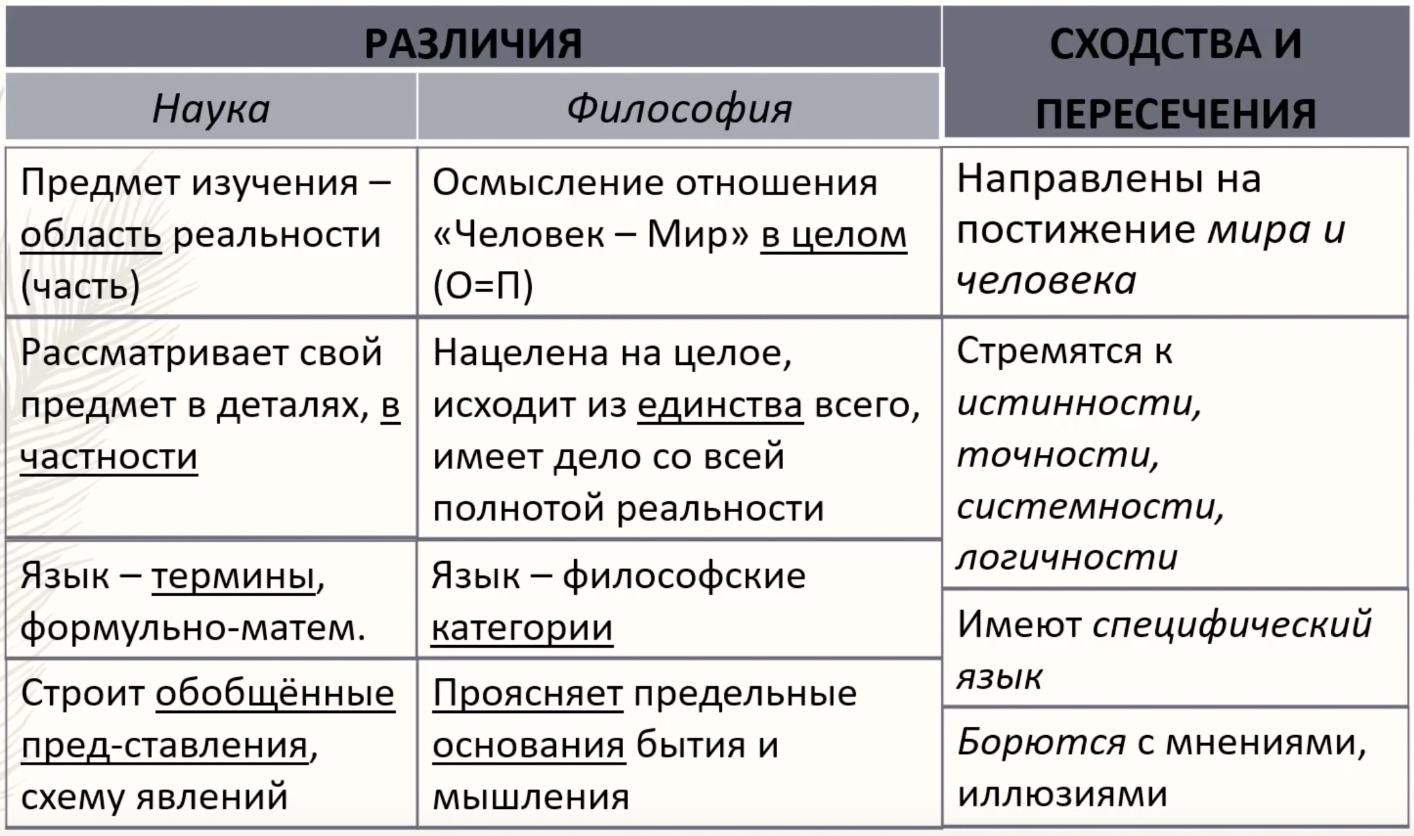
\includegraphics[width=0.8\linewidth]{pictures/sciphil.png}
    \label{sciphil}
\end{figure}

% Каждая наука выделяет в качестве предмета изучения определенную область реальности.
% Философия же занимается осмыслением отношения человек-мир в целом.  Сходство в том, что объект у этих видов культуры один --- действительность или то, что есть. 

% Философия нацелена на целое,
% в которое к тому же не только мир включается, но и мы сами во всей полноте и
% парадоксальности с плохим и хорошим и мира и нас. Поэтому объектом философии,
% который совпадает с предметом, является прежде всего отношение человек-мир в
% целом. 

% И различные философские концепции, а также настроенные в их свете
% умонастроения людей в различные культурно-исторические эпохи базируются именно
% на различном осмыслении этого отношения. Многие же, поскольку нацеливаются на
% формирование знания, вынуждены в свете этого целостного настроения вдаваться в
% подробности, детали, частности, то есть из всего в целом выделять для своего
% изучения предметы. Так в отличие от философии, представляющие в нас возможность
% и необходимость иметь дело с целым, каждая частная наука имеет в качестве
% предмета своего изучения какой-то кусочек реальности, какую-то часть целостного
% отношения человек-мир. Лингвистика язык, биология живую природу, химия состава
% превращения веществ, социология, человеческое общество и так далее. Наука по
% сравнению с философией избирает путь части, в том числе разбора на части,
% представления своего предмета как части реальности не в целостной слитости со
% всем остальным, а в его выделенности в частности. Несмотря на такие различия в
% нацеленности и философии и наука стремятся к истинности, точности, системности,
% логичности. Хотя требования, например, истинности суждения ученого-философа
% может пониматься несколько по-разному, невозможно себе представить, чтобы
% философские поиски и научные исследования ввели стремление к ложности. Здесь
% истина объединяет скорее даже не как эпистемологическая категория, но как
% этическая, поскольку выбор истины в противоположность лжи, прежде всего выбор в
% ту сторону, что мы считаем благом. Для своих различных задач, философии, как
% имение дела с целым, и науки, как познание аспектов реальности в частности, у
% данных видов человеческой деятельности, безусловно, имеются различные способы
% подхода к своим задачам и их решениям. Несмотря на то, что мыслительные операции
% мы производим как в науке, так и в философии одинаково, постановка, проблема,
% анализ, синтез, сопоставление, выделение общего и особенного, систематизация,
% формулирование выводов и так далее. Язык науки и философии различаются
% достаточно сильно. Каковы же языковые инструменты, используемые для выражения
% научной мысли, в отличие от философска. Этого мы касались в первом вопросе
% предыдущей темы, когда говорили о коммуникативных аспектах науки. Основы
% научного языка составляют особые понятия, которые называют терминами. Примеры мы
% тоже приводили, но давайте из разных наук еще повспоминаем вектор, рецептор,
% электроли, социальная группа, девиантное поведение, себестоимость, литерация и
% так далее. Помимо отсутствия в них экспрессивности, эмоционально ценностной
% окраски, первое, что также бросается в глаза, это точность терминов и
% стремящаяся к максимальной однозначности референтность, то есть строгое
% соответствие слова, словосочетания, наблюдаемому в реальности или так
% называемому идеализированному объекту, которым пользуется абстрактное научное
% мышление, например, материальная точка, абсолютно черное тело и так далее. В
% отличие от терминов в научном языке для философского основу составляют категории
% добро, красота, истина, свойства, структура, части целого, количество, качество,
% закон, уникальное, универсальное и многие подобные слова составляют несметный
% список философских понятий. Почему? Их нельзя поставить в один ряд с научными
% терминами. сделать это невозможно, как раз потому, что эти слова не имеют
% определенной референции в реальности, но задают сами условия нашей понимающей и
% исследующей работы с реальностью. Имеется в виду не то, что, не знаю, девиантное
% поведение, например, реально наблюдается, а красота или часть, нет. Речь о том,
% что у прекрасного и безобразного части и целого движения и покоя и так далее
% может быть совершенно различное смысловое наполнение, различное ценностное и
% этическое окрашивание в зависимости от тех мировоззренческих оснований в свете,
% которых мы называем нечто прекрасное, сопоставляем части целое, определяем в
% качестве движения или покоя. А, например, катет прямоугольного треугольника
% остается термином для его стороны, прилегающий к прямому углу со времен
% древнейших геометров и на протяжении истории науки свое значение не меняет. Мы к
% этому вернемся с вами сегодня в следующем вопросе и на примере категории части и
% целого рассмотрим, как их смысл различается в разные эпохи в зависимости от
% философских оснований каждой культурно-исторической локальности. Что же касается
% в этом плане сходств, несмотря на то, что в языковом плане наука и философия
% используют различные средства, объединяет их факт выражения своей мысли на
% особом языке, отличном от обыденного. Хотя философия во многом ближе к обыденной
% речи, чем наука, и всматриваться в естественный язык как в отражении оснований
% человеческого миропонимания, все же она с предельной строгостью говорит на языке
% понятий, которые в обыденной речи лишь интуитивно подразумеваются. Точнее, было
% бы сказать, что философия в этом плане имеет специальную цель разворачивание
% предельных смыслов понятий, в то время как обыденный язык их интуитивно как бы в
% свернутом, нераспакованном виде использует для цели коммуникации. И вот отличие
% языка науки от повседневного естественного языка еще более очевидно. На огромную
% долю наука в ее стремлении к установлению функциональных связей приходит в
% область искусственного языка, это прежде всего язык математики. Безусловно,
% обыденный язык, особенно в современности, в многом, благодаря СМИ, выхватывает
% научную лексику, вовлекая ее в коммуникацию. Однако, как и в случае с
% использованием философских понятий, от него не стоит ожидать строгого
% соответствия терминов их научным значением и глубокого четкого понимания сути
% явлений, так привлекательно умно названных наукой. И еще один пункт в нашей
% табличке давайте отметим, что мы имели в виду, когда определяли науку как теорию
% действительного. Тут предполагается ответ на два вопроса. с чем и как наука
% имеет дело, когда формируют знания. Наука имеет дело с предметами реальности. С
% беспредметностью наука не работает. Однако, то, что может в той или иной
% ситуации быть для человека совершенно не в предметном статусе, наука также
% способна делать предметы. Например, ощущение для художника, который его
% разворачивает в своей смыслополагающей деятельности, совершенно не то же самое
% ощущение, которое у этого художника наблюдает психолог. Для исследователя это
% предмет изучения, предмет психической реальности. А для художника этот один тот
% же феномен имеет значение не в качестве предмета, а в состоянии переживания, в
% котором он творит, и ему дела нет до того диагноза, который ставит ему психолог.
% И второй момент в нашем суждении то, что нереально науку не занимает. Даже
% виртуальная реальность, которой, на первый взгляд, в мире нет, на самом деле в
% какой-то мере реальность имеет место в нашей действительности и, надо сказать,
% немало на нашу актуальную реальность влияет. Поэтому к ней у науки информатики,
% кибернетики, психологии, социологии, математического моделирования и так далее
% проявляется не меньше интерес, чем, например, к природной действительности. А
% вот единорогам и русалкам ученые в реальности отказывают, поэтому, если ими и
% занимаются, то только как предметами фольклора или эстетическими образами
% филологии и науках об искусстве. Следующий вопрос, как наука со своими
% предметами имеет дело? Она их представляет, ставит перед собой. Как можно
% предмет научного исследования поставить перед собой? Не говоря уже о зрительно
% ненаблюдаемых для психолога феноменах психики или взаимодействующих молекулок у
% химика, даже медик, перед которым стоит человек, пациент, не может физически
% поставить перед собой человека вообще. Да, исследует тело он сейчас у
% конкретного человека, а у химика сейчас в колбе идет конкретная реакция. Но
% конкретными вещами ученые могут заниматься только в свете представления о
% человеческом теле вообще, о психике вообще, о химической реакции вообще. Наука
% не в первую очередь имеет дело с уникальным. На самом деле, каждый раз
% уникальным человеческим телом, психикой, животным, веществом и так далее. А с
% уникальным только как вариация воплощения универсального. Причем универсальное,
% общее, сходное, почему-то для науки важнее. Единичного, уникального,
% индивидуального. Между тем, как каждая конкретная вещь явилась ученому и самим
% исследователям, всегда прочерчивается экран обобщенного теоретического
% представления, которое абстрагирует или выделяет в уникальное, универсальное
% посредством наложения на уникальную, мыслимой, универсальной форму. Что же
% философия? Ее цель не составление знания о действительности, а прояснение
% предельных оснований бытия и мышления. И тофтологически, философия сама себе и
% цель и средство. Например, известнейший мыслитель XX века Мартин Хайдегер дает в
% своих лекциях такое определение «философия есть философствование». То есть,
% философия занимается осмыслением, пониманием, смысла всего в целом и продуктом.
% Такой деятельностью может быть только тоже мысль, понимание. Никакой другой цели
% у философии нет. Нет и никакого другого продукта. Это осмысление ради
% осмысления, собственно, человеческая деятельность. И если вам говорят, что
% философия имеет цель на первый взгляд нечто иное, например, научить чему-то или
% что-то воспитать, то имеется в виду научить мыслить или воспитать культуру
% мысли, но вовсе не научить жить, не научить какому-то мировоззрению, не научить
% мудрости. То есть, еще раз, главная задача философии не выдать какую-то
% информацию, а разработать и дать человеку инструменты осмысления, побудить его
% задаваться собственными вопросами и искать истину. Что же, в науке разве ученые
% не этим занимаются? В том-то и дело, как исследователи мы тоже осмысляем, но в
% рамках профессиональной деятельности ученого мы берем эти инструменты и в свете
% истины что-то видим, изучаем в своих объектах. А как философы мы как бы
% оглядываемся на то, благодаря чему есть то, что перед нами, на сам свет истины,
% который как бы у нас за спиной, когда мы познаем. Мы рефлексируем свою
% деятельность и даже если по профессии занимаемся наукой, это не значит, что в
% нас, как в живых человеческих существах, не присутствуют философские способности
% к видению мира в целом, постановки под вопрос даже устоявшегося знания и
% пониманию первопричин происходящего. Так вот, общее. Для философии науки мы
% уловили, должен рождаться смысл, должна присутствовать истина. Не только
% философия в своей, смыслопорождающей деятельности, борется с мнениями и
% иллюзиями. Науке не в меньшей степени приходится совершать усилия отделения
% научного знания от уже научного типа снежного человека, инопланетян,
% рептилоидов, экстрасенсов и так далее. Понятно, да? И объяснять в своих строгих
% формулировках научные законы в противоположность расхожим обыденным их
% трактовкам и неточным интерпретациям. Вы это, как ученые, прекрасно знаете по
% себе. Например, если мы скажем, что электроны вокруг ядра атома движутся по
% орбитам разной формы, сферическая, гантелеобразная или сложная в виде цветочка,
% химик или физик элементарных частиц нас поспешит поправить. Электроны, нельзя
% сказать, движутся вокруг ядра, тем более, конечно, не представляют собой эти
% орбиты. Объемные рисуночки, сферические, гантелеобразные, это условное
% изображение плотности вероятности наиболее вероятного пространства, опять же, в
% кавычках, нахождения электрона в том или ином энергетическом состоянии вблизи
% ядра. Не точка в пространстве с определенными координатами, а одновременно и
% волна, он как бы размазан по этой вероятной области. И вообще, давайте я вам
% покажу, откуда это все берется, обратимся к решению уравнения Шрюдингера для
% волновой функции. И понеслось. Ученые обязаны нас поправлять, возвращать из
% размытости обыденного представления на рельсы научного знания, иначе мы
% ориентироваться в мире будем по мнениям, то есть по мнимости, а не по точному,
% теоретическому. Философы по-своему борются против мнения, расхожих представлений
% и стереотипов. С их точки зрения, не специалисту простительно, например, иметь
% смутные представления об элементарных частицах, но непростительно, скажем, не
% рефлексировать навязываемые со стороны стереотипы о выборе профессии или о том,
% должно ли счастье быть общепринято. Но, в принципе, совершается сходное движение
% через объяснение, показывание ложности и губительности для нас таких
% недопроясненностей, готовых схем, удобных решений. 



\subsubsection{Наука и религия}

\begin{figure}[H]
    \centering
    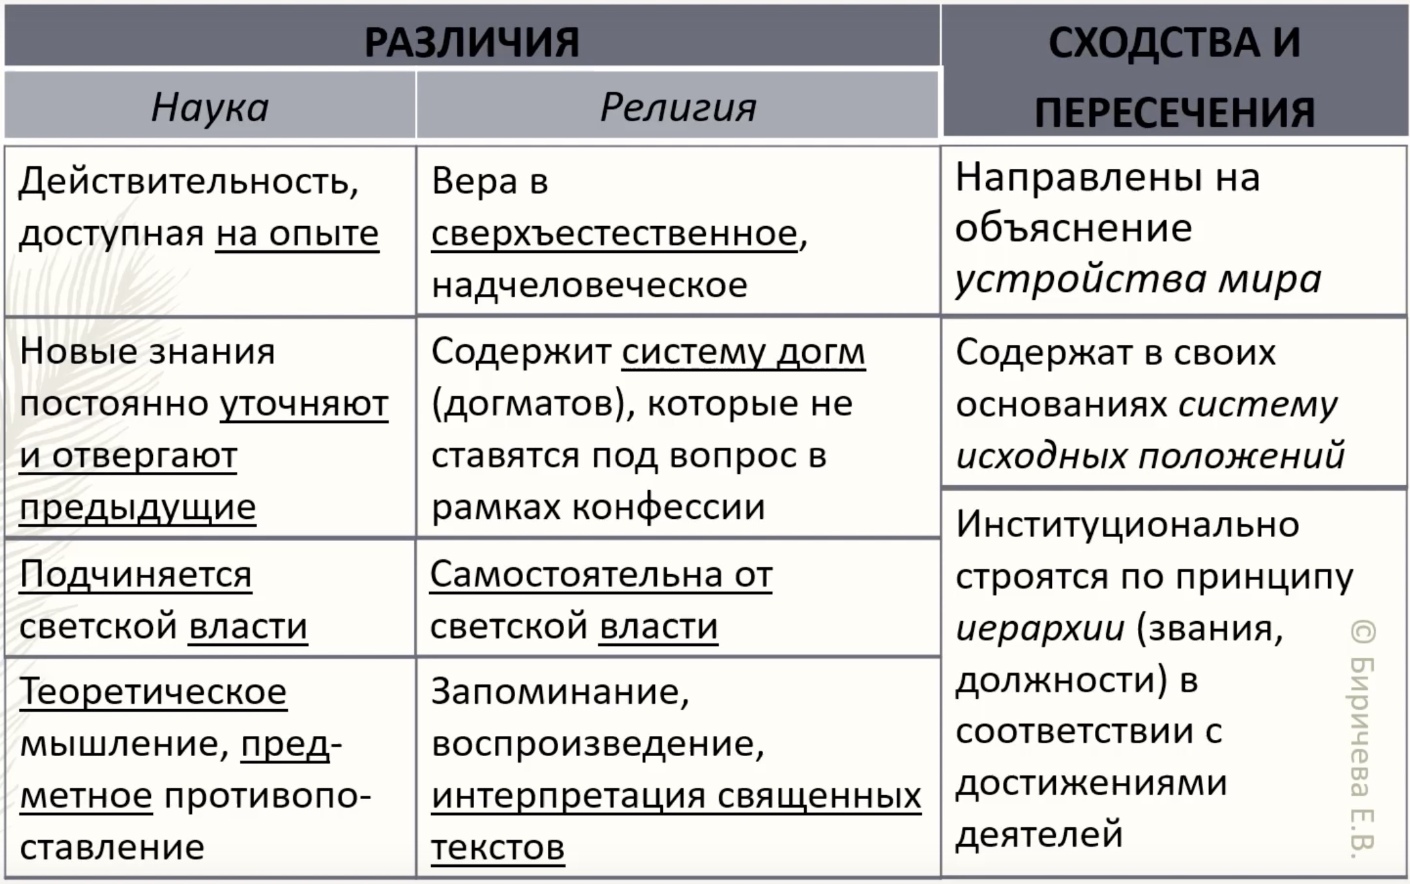
\includegraphics[width=0.8\linewidth]{pictures/scirel.png}
    \label{scirel}
\end{figure}

%  Прежде всего, отметим,
% что наука изучает объекты и явления действительности, которые доступны на опыте.
% Религия же основана на вере в сверхъестественное и трансцендентное, то есть
% антелеком посвящена незримым, высшим основаниям всего. А наука, как мы только
% что проговорили, сопоставляет с философией, имеет дело только с тем, что дно,
% что мы можем реально в мире встретить. Но, безусловно, оба эти вида культуры
% каждый по-своему объясняют первоосновы мира и трактуют как-то специфику
% человека, как внутримирного существа. Тут бегло заметим, чем религия отличается,
% в том числе, от мифологии, чтобы вы не путали. В мифе, конечно, есть
% представление о сверхъестественных силах, но, помимо этого, там намешаны и
% элементы других феноменов культуры, повествования о богах и героях, как
% эпические, литературные произведения, какие-то рецептурные рекомендации по
% поводу обустройства быта, философские концепции, так или иначе, трактующие
% благо, справедливость, природу, материя, способ возникновения мира, в жизни
% человека. Ну, понятно, да? Любая религиозная система концентрируется только на
% представлении надмирового, надчеловеческого, божественного, причем не
% обязательно бог один, не обязательно это сверхъестественное персонифицируется и
% не обязательно, кстати, божество вне мира мыслиться, то есть индуизм, даосизм,
% синтоизм и многие другие системы это тоже религии, а не мифологии, хотя, еще
% раз, может не быть антропоморфного божества, их может быть много и они могут
% мыслиться присутствующими в мире, а не вне его. Естественно, из этих
% представлений можно логически выводить какие-то этические рекомендации, советы
% по устройству быта, но это уже будут богословские, научные или философские
% интерпретации. Чего? Это второе главное отличие от мифологии священных текстов,
% которые содержат догмы или догматы, нерушимые и неотменимые в рамках
% соответствующей системы основоположения. Миф текуч, в нем возможны в самом
% разнообразные добавления, искажения, интерпретации при передаче из уст в уста.
% Любая конфессия фиксирует, свои базовые положения закрепляют священных текстов.
% И очень много усилий надо приложить, чтобы какой-то новый догмат ввести в эту
% систему. С огромным трудом подобное, например, удалось сделать в православии в
% XIV веке Григорию Паламе. Он предложил в противоположность католическому учению
% разделять понятия энергии и сущности в отношении Бога и его деяний. А вот
% скажем, такой шаг в сторону сближения с исламом, как иконоборчество, в
% православии в свое время потерпел неудачу. Вокруг этих ожесточенных споров
% творились поворотные исторические события, заключались под стражу и гибли люди.
% Так что религия четко держится своих догматов и немногочисленные случаи их
% изменения скорее исключения, чем правила. В отличие от этого, наука развивается
% путем постановки под вопрос действующих знаний и производства новых, уточняющих
% или преодолевающих предыдущие. Со второй темы можно здесь вспомнить
% постпозитивистов Карла Поппера и Тома Сакуна, которые по-разному предлагают
% рассматривать развитие науки эволюционно или путем научных революций. Но
% сходятся они в том, что все-таки со временем одни научные теории и подходы
% заменяются другими. Тем не менее, нельзя отрицать, что как наука, так и религия
% в любом случае содержат в своем основании систему исходных положений. Просто
% внуки они периодически пересматриваются, а в религии если пересматриваются, то
% возникает новая конфессия отдельно на своих основаниях и становится
% равноправными другими. Так, когда-то единое христианство разделилось на
% православие и католицизм, а затем от последнего отмежевался протестантизм в
% различных вариантах лютеранства, кальвинизма, англиканства и так далее. Об этом
% в темах о средневековье и возрождении вам подробно расскажет Светлана
% Викторовна. Какие еще отличия можно выделить? Обычно религия в современном мире
% существует автономно от власти, то есть давайте применять разобранные в
% предыдущей теме термины, институция анализируется в качестве самостоятельной по
% отношению к светской власти системы. А вот наука чаще всего входит в эту
% систему, подчиняется. Например, мы с вами на прошлой теме говорили, что
% Министерство науки и высшего образования РЭП занимается управлением и сельской
% деятельностью. Что касается в этом отношении сходств, институты науки и религии
% строятся по принципу иерархии должностей, званий, рангов, служителей или
% сотрудников в соответствии с достижениями каждого деятеля. То есть
% институционально предполагаются как в научном, так и в религиозном сообществах
% системы соподчинения и иерархического расположения в зависимости от тех или иных
% показателей, которые к тому же оцениваются специальными внутренними инстанциями.
% Наконец, в плане когнитивной специфики исследовательская работа предполагает
% теоретическое мышление, представляющее предметы в качестве противопоставленных
% знаний ученого. В религиозных практиках распространены в первую очередь
% запоминания, передача основ учения через религиозное обучение и интерпретация
% священных и авторитетных текстов. Также неотъемлемой составляющей являются
% строго регламентированные ритуалы, обряды, священодействия. В науке аналогом
% можно называть, пожалуй, соблюдение металлогических процедур, однако ввиду того,
% что они сами трансформируются, меняются, уточняются, изобретаются новые и так
% далее. Не факт, что это пойдет в рубрику сходства. Вообще наука и религия в
% современном мире достаточно полярные позиции, занимают по отношению друг к другу
% и трудно выделить много пересечений для них, глаза бросают скорее различия. Но
% думаю, того, что мы тут отметили, достаточно для представления экзаменей.

\subsubsection{Наука и искусство}

\begin{figure}[H]
    \centering
    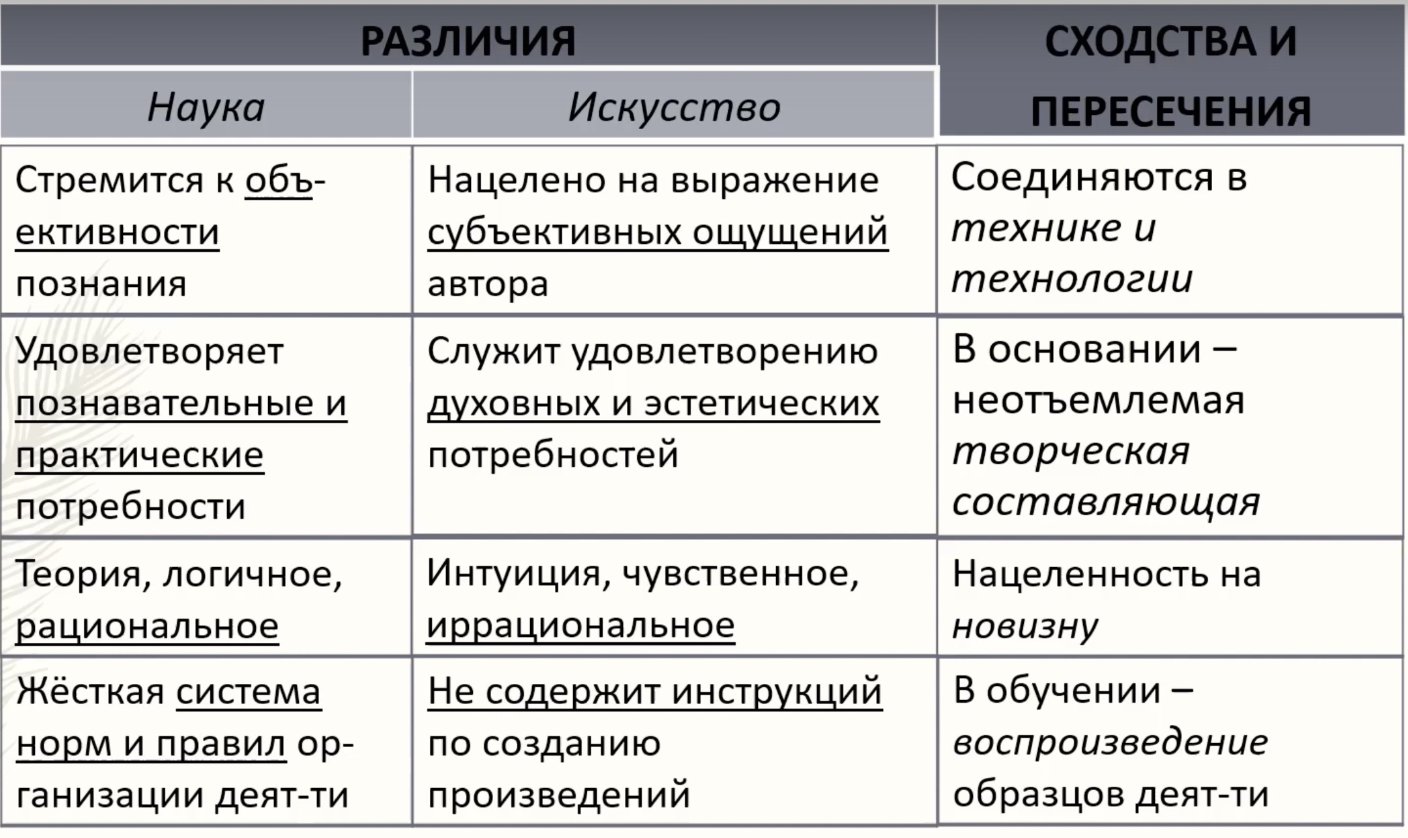
\includegraphics[width=0.8\linewidth]{pictures/sciart.png}
    \label{sciart}
\end{figure}

% поэтому перейдем к последнем сравнению, наука и искусство, чем у нас различаются
% и в чем сходятся. Тоже достаточно неблизкими друг другу кажутся эти виды
% культуры. Первое отличие, которое сразу приходит на ум, заключается в том, что
% наука стремится к объективности выражаемого знания. Тут объективность можно в
% двух смыслах брать, как отражение реальности самой по себе, представление его
% обобщенных законов и как противоположное субъективному, личному, то есть не то,
% что одному и не виду показалось, а что разделяется большинством в плане
% интерсубъективности. Искусство же не особо интересуется универсальными
% закономерностями и достоверным их описанием, а нацеливается на выражение
% субъективных переживаний и ощущений автора, его уникальной точки зрения, его
% новаторского способа видеть, пусть и ту же самую реальность. Пересекаются наука
% и искусство в технике и технологии. Это мы уже отметили, выше говоря, о
% древнегреческом слове техно, которое означает искусство в широком смысле как
% специфическая человеческая деятельность, направленная на создание того, что не
% рождается и не живет само по себе, но требует нашего осмысляющего участия. В то
% время, как наука направлено на удовлетворение мировоззренческих, познавательных
% и практических потребностей, искусство служит удовлетворению духовных и
% эстетических потребностей человека. Но и там, и там лежит в основании
% неотъемлемая творческая составляющая. Иногда кажется, что искусство это наиболее
% творческая деятельность, но на самом деле, во-первых, в искусстве огромную долю
% занимают те же самые коммуникации и рутинная работа, как и в науке, когда надо
% отточить мастерство, тренироваться, набить руку, много чего прочитать, обсудить
% с коллегами и так далее. А во-вторых, исследователь не менее творец, чем
% художник, просто он создает новое знание или техническое изобретение, а не
% картину или образ, скажем, спектакля. То есть, креативные способности можно в
% любой деятельности равно проявлять. При этом в науке мы опираемся на
% рациональные, логические, теоретические способности, а в искусстве большее
% значение имеет опора на интуитивные, чувственные и рациональные способности
% человека. Но, конечно, как и любая творческая деятельность наука и искусство,
% каждая по-своему нацелена на новизну. Наконец, можно такие еще различия
% предположить. Если наука имеет систему норм и правил ведения научного
% исследования, строгий язык, логику и так далее, то искусство не содержит
% однозначных инструкций по созданию произведений. Тем не менее, в обоих случаях
% обучение предполагает изучивание техник работы и задания на их практическое
% применение воспроизводства созданного ранее. Как, например, химику надо
% проделать множество лабораторных работ, воспроизводящих уже известные синтезы,
% аналитические процедуры и технологические процессы. Так и, скажем, скульптор
% сначала обучается слепить череп, вырезать барельеф, нагончарить кружку, а потом
% уже придумывает свой абсолютно новый шедевр. И далее, по подобной схеме вы
% самостоятельно на основе своих эрудиций и жизненного опыта сможете сопоставить
% науку с чем угодно, потренируйтесь на семинаре, это сделать по поводу
% образования, морали, политики и других феноменов культуры. 

\section[Культурно-исторический контекст развития науки и его философские основания]{Культурно-исторический контекст развития науки и его философские основания
(онтологические, гносеологические, этико-аксиологические)}

\subsection{!!! Понятие культуры в связи с её фундаментальными основаниями}

Культурология
знает, ведает, безусловно, чрезвычайно много о культурах, но сколько я не читала
труды исследователей в этой области, находила только поверхностные определения
культуры, не в смысле плохие, но замечающие только внешние проявления, все то,
что у нас обычно и ассоциируется с культурой, традицией и ценностями. Это все
замечательно. 

Однако, такое знание, хотя, несомненно, важно, интересно и для
определенных целей полезное, ничего не говорит о том, почему сложилась именно
такая культура, почему не другая, почему не иначе. Говорить, что так исторически
сложилось, или потому, что такой менталитет, или благодаря такому особому языку,
значит, повисать над бездной.
Мы всегда можем дальше спросить, а почему так
сложилось, почему такой язык и менталитет, на каком основании? 

Это только
философия может помочь, поскольку именно она занимается прояснением предельных
оснований человеческого бытия и мышления. И, по сути, понимание особости каждой
культуры делая ответы на тот же философский вопрос о своем собственном, которым
мы задавались на предыдущей теме, говоря об индивидуальном в человеке. 

Культуры отличаются своими традициями, идеалами, нормами, ценностями,
которые, в свою очередь, выросли из своего собственного, каждой культуры. Они
сформировались в свете определенного способа бытия, образа организации жизни.
Что значит способ бытия? это образ мысли, способ видения мира и себя в нем,
способ понимания окружающей действительности, в русле которого мы выстраиваем
свои отношения с миром, с природой, с другими людьми, с теми же продуктами,
имеющиеся культурой, в которой рождаемся. 
Поэтому мы и говорим, что философское
определение культуры это способ бытия, а именно в случае человеческой культуры
способ понимания человека мира и своего положения в нем, в свете которого
выстраивается определенное отношение к окружающей действительности,
результирующиеся в выработке норм и идеалов человеческой деятельности. 

Когда я
говорю об основаниях, как о способе бытия, я имею в виду, что оснований нет в
виде какого-то определенного что. Мы знаем, что исторически меняются содержание
научного знания, нормы и идеалы в искусстве появляются и уходят со сцены
религиозной системы и так далее. Надежное основание возможно только не
субстанциально в форме как образа действия или способа бытия. Конечно, плюрализм
или множественность оснований и в форме как, очевидно, в случае каждого
человека, но надежен для меня только мой способ бытия, другой не может быть за
меня моим способом, хотя с содержаниями мы можем с одинаковыми иметь дело.

Способ как конкретный путь, образ действий, по определению единичен, целостен и
уникален, то есть своей особостью и будет отличаться от других способов, но он
не зависит от того, на материале каких содержаний действует, он как-то поступает
со всем, что ему дано, что-то видит, что-то игнорирует, что-то использует, что-
то нет и так далее. На основании чего мы что-то делаем, видим, используем. Не
потому, что так принято или все вокруг считают это ценным. Мы можем поставить
это под вопрос и заменить одни говорят одно, другие другое, третье, третье. Кому
поверить? Почему надо вот это делать, не вот это? Что реально, а что иллюзорно?
Почему я к этому так отношусь? На подобные вопросы мы даем каждый пропускать
через себя, думавая по-своему, на материале, личностной истории и в свете своих
уникальных склонностей, способностей, наполняя смыслом, даем свои ответы. 

Мы
отталкиваемся от своего фундаментального основания, которое неизменное, а не
имеющимся из стороны в сторону, гонимые то одним, то другим чем-то мнением и не
слепо автоматически делаем, как принято. Иначе бы основания не переосмыслялись и
эпохи бы не менялись, и культура была бы у людей одна одинаковая по всему
земному шару. 

И вот точно так же, рефлексируя по направлению к основанию
культуры, мы приходим к необходимости прояснить самые фундаментальные из них,
то, в связи с чего мы мыслим и поступаем в бытии, речь об онтологических
основаниях, в контексте которых также возможным становится прояснение и других
философских оснований, гносеологических, этических, аксиологических и так
далее. Тогда, парадоксальным образом, философия у нас становится философией и
культурой, ведь именно прояснением этих оснований, понимания всего в целом, а у
разных культур они разные, мы занимаемся.

\begin{figure}[H]
    \centering
    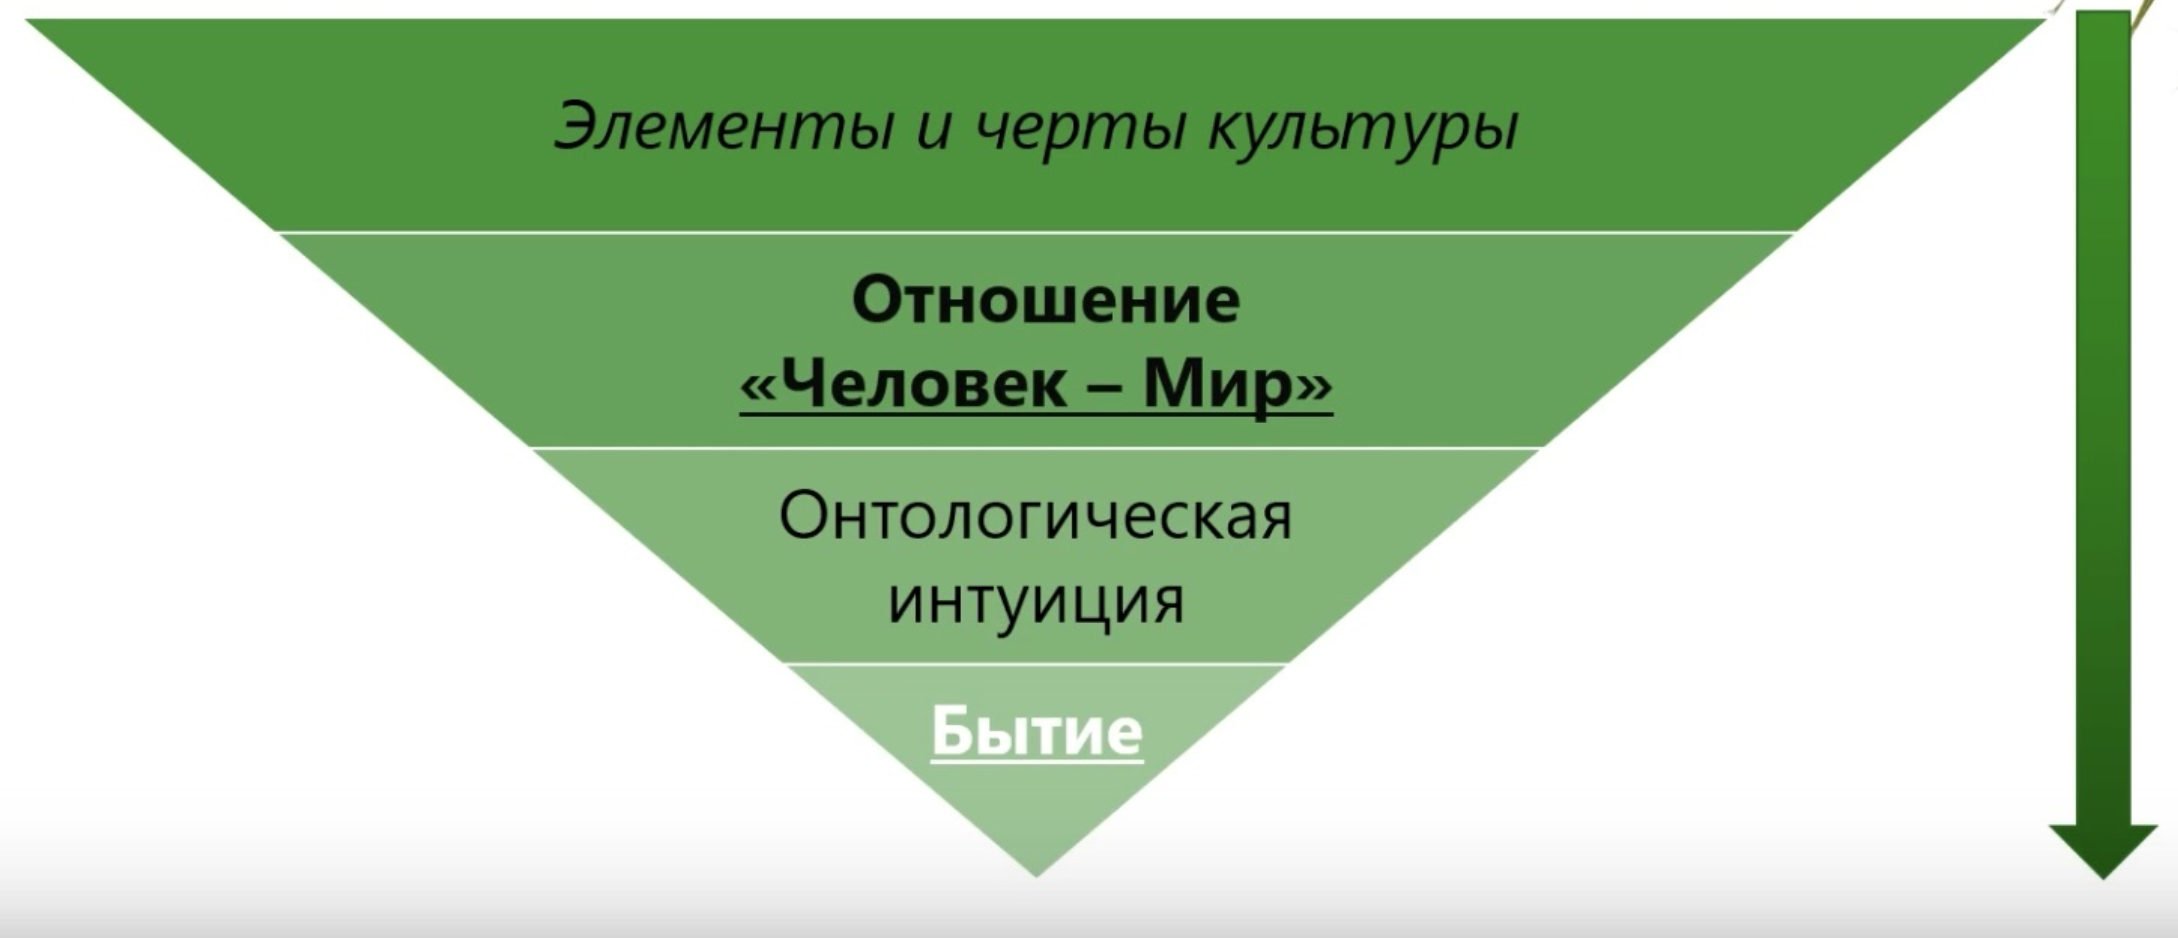
\includegraphics[width=0.8\linewidth]{pictures/hz.png}
    \label{hz}
\end{figure}

% В ротивоположность чему выстраивается способ бытия? причем каждый
% раз различный в исторической перспективе у представителей разных современных
% культур, в пределе у каждого человека.
% Бытие противоположно
% небытию и способ быть выстраивается вопреки или в ответ на страх небыть. То есть
% в основании нашего бытия предельным образом лежит на самом деле небытие,
% которого мы боимся, поскольку знаем о своей конечности и отталкиваясь от угрозы
% небытия стремимся быть максимально добротно быть, достигать пункты своего
% существования. Эту идею, причем применительно к осмыслению культурно-
% исторических трансформаций мировоззрения, проводит в своей книге «Муж что быть»
% выдающая немецкий мыслитель Пауль Тилли. тревога небытия постигается нами в
% глубоком детстве, обычно в возрасте от 3 до 5 лет, когда мы начинаем осознавать
% свою конечность во времени и пространстве. В пространстве мы познаем границы
% своего тела и то, что не можем по своему желанию непосредственно оборудовать
% другими людьми и внешними обстоятельствами. Безусловно, временность нашего
% существования каждым переживается как просто страх смерти. Однако, даже в языке
% есть такое выражение «Может быть что-то страшнее смерти». И вот для каждого
% человека в той совокупности окружающих его условий, в которой формируется его
% личность, то, что страшнее смерти, переживается уникальным образом и
% сворачивается с глубокого детства интуитивно в ту или иную форму угрозы небытия,
% чего, как вы думаете, можно бояться сильнее смерти. Например, хаоса и
% неупорядоченности, бессмысленности своего существования и окружающего мира,
% тотальной необеспеченности человеческого положения, возможности не оправдать
% ожидания окружающих людей, поступить не по совести, отказаться отделенным от
% всех, одиноким и так далее. Противоположность каждый раз конкретной форме угрозы
% небытия каждый человек выстраивает свой способ быть. Например, опасаясь хаоса,
% человек будет упорядочивать и рационализировать, структурировать и
% систематизировать все вокруг. Страх и необеспеченности логично развивать
% медицину и экономику, стараясь использовать природу на службу человека,
% удовлетворяя потребности и пытаясь продлить жизнь. Если человек боится не
% оправдать ожидания других людей, то посвятить себя благородному делу, вежливо и
% учтиво со всеми будет обходиться, учитывать интересы и особенности других людей,
% стараться соответствовать тем месту и роли, которые за ним закрепляются в
% социальной структуре и так далее. Тут, когда мы говорим о культуре, надо не
% забывать как раз о том, что культура как такой способ бытия не определяется
% географическими или национальными границами. Безусловно, языковая, социальная
% среда, историческая память, экономико-политическая ситуация связывают общность
% условий. Однако, это не детерминирует нас полностью, и мы можем принадлежать
% разным типам культур с ближайшим соседом, но почувствовать родство с человеком с
% другой половиной земного шара. Бредом, конечно, далеко не все люди осознают
% собственную тревогу небытия, да и кризисные моменты нашей жизни могут
% существенно повлиять на смену типа фундаментальной тревоги. В этом случае нам
% придется кардинально пересмотреть основания своих поступков, скорректировать
% характер, разменить жизненные цели и ценности. в графических регионах можно
% говорить лишь о преобладающем типе культуры. Наконец, последний момент,
% наверное, вы почувствовали культуру тревоги, хаоса и неупорядоченности, та, что
% исторически выросла на западноевропейской почве. Именно ее традицию внуки и
% философию мы, собственно, должны разбирать в нашем курсе. С ней заодно очень
% близко идет культура тревоги необеспеченности, как мне кажется, навязываемая
% сейчас ему миру со стороны США. В рамках глобализации сегодня мы, в смысле
% представители остальных культур, испытываем на себе влияние и, я бы даже
% сказала, давление со стороны этих двух типов культур, действующих совместно в
% плане стандартизации и универсализации, в том числе в сфере науки, в плане
% экономического расхода всего на планете, мечтания определения жизни, бессмертия,
% комфортного существования и подобных вещах. Это неплохо и нехорошо, просто важно
% понимать, откуда у современной науки ноги растут. Но важно не забывать, что в
% мире есть еще множество типов культур, в том числе наша тоже особенная. И нет,
% на ни хуже, ни лучше другой. Мы равноправны, поскольку каждый чувствует в той
% или иной форме экзистенциальную тревогу небытия и каким-то образом ей конкретно
% отвечают в своей ситуации, своим способом. способы не лучше и не хуже друг
% друга, потому что просто-напросто каждый хорош в отвечании на свою угрозу
% небытия и, понятное дело, плох, если им пытаться отвечать другому
% фундаментальному страху. В частности, поэтому на отечественной почве, как вы
% сплошь рядом видите, не проживаются решения, может быть, полезной и
% рациональной, но органично выросшей на почве иных культур. Таким образом, теперь
% мы в данной теме о культуре сможем заложить для себя фундамент понимания
% существа культурно-исторических эпох. Для этого опишем в логике культуры как
% способа бытия методологию, с помощью которой мы будем двигаться в темах
% следующего раздела, который называется «История науки в ее связи с философией»,
% начиная изучение каждого типа науки с прояснения его культурно-исторических
% условий и философских оснований соответствующей эпохи. Здесь также необходимо
% кратко привести конкретные примеры, какими были основания культурно-исторических
% эпох, которые нам предстоит изучать, чтобы стало хоть немного понятнее, как
% различное содержательное наполнение, ну, какое, да, наполнение могут получить
% основания и в соответствии с ними тип науки. Итак, антологические, сущностные и
% бытийные основания. Это фундамент определенного типа мышления, добираясь до
% которого сквозь все внешние наслоения, ну, там, традиции, социально-политические
% условия, ценностные ориентиры, мы как раз получаем ключ к пониманию оснований
% мышления, неважно, конкретного человека или культурно-исторической эпохи. Хотя у
% каждого из нас уникальное представление о себе, о мире и о своем месте в нем,
% если мы говорим о культурно-исторической эпохе, даже такой длительной, как,
% например, античность или средневековье, каждое существовало более тысячи лет, то
% имеют место тенденции примерно одинакового понимания этих базовых моментов всеми
% членами данного общества, сформировавшись в определенный момент, целостные
% представления о мире и человеке безусловно отражаются в языке соответствующей
% культуры, а с языком передаются в ходе воспитания от родителей и детям, то есть
% последующим поколениям. Поэтому смена культурно-исторических эпох происходит
% медленно, для с целыми столетиями. В связи с этим, например, так сложно провести
% разделительную черту между окончанием эпохи античности и началом средних веков.
% христианское мировоззрение, легшее в основу средневекового миропонимания, начало
% формироваться как минимум за четыре столетия до того, как оно получило тотальное
% распространение в Европе, сменив собой окончательно античный тип мышления. Так
% вот, сущностные основания того или иного типа мышления как раз предполагают
% определенное понимание отношения человек-мир, которое содержательно отличается
% для каждой эпохи. Одушевленная, упорядоченная, но при этом движущаяся,
% изменяющаяся вселенная античности с отражающим ее целостность и полноту
% человеком совершенно не совпадает со средневековым иерархически сотворенным по
% замыслу Бога миром, в котором человек уже чувствует себя иначе, в частности,
% например, не имеющим права на преобразование вещей мира, на буйную творческую
% активность и праздновать развлекательный образ жизни. Что касается бытийных
% оснований, естественно, во всей эпохе далеко не все люди настолько глубоко их
% для себя осмысляют и проговаривают, чтобы дойти до самой фундаментальной основы
% своего способа мысли, до понимания категории бытия. Категория бытия, то,
% благодаря чему все есть и есть именно так, представляет собой как бы пустую
% форму, наполнение которой в рамках каждого типа мышления также происходит по-
% разному. Однако нам в ободенной жизни достаточно интуитивного ее понимания,
% которое, опять же, в ходе воспитания нами усваивается. На этом основании мы
% сами, не задумываясь об этом, строим свои суждения и из этого основания выводим
% свои представления о действительности. На этом основании действия мы поступаем
% именно определенным образом. Прояснить и проговорить эти предельные основания
% всей нашей культуры, чтобы понимать, на чем все основывается, как раз задача
% философии и философов. Они занимаются профессионально глубокой рефлексией, то
% есть вопрошением о причинах, в пределе о первых причинах всего сущего,
% устройством мира, определенным способом мыслить и так далее. На самом деле все
% люди являются стихийными философами, поскольку периодически задаются вопросами о
% причинах стихийных событий, но большинство в силу посвящения себя иным занятиям
% не практикуют рефлексию настолько глубоко до бытийных оснований, особенно для
% нас исследователей это очень полезно для того, чтобы четко для себя понимать
% основания своих научных суждений и выводов теорий. Поэтому мы обучаемся
% философии и знакомимся с помощью ее метода с историей нуки. Так вот,
% антологическим основанием является помимо понимания отношений человек мир
% интуитивное понимание бытия. Здесь под интуицией имеется в виду не шестое
% чувство, а образ мысли, складывающийся в свете того, что остается для нас
% самопонятным, безусловным, несомненным, короче говоря, тем, что не ставится под
% вопрос. Это безусловный фундамент, от которого отталкивается любая наша мысль,
% то, что далее не может быть рефлексировано. Так, забегая вперед, для современной
% нашей эпохи, пожалуй, можно условно сформулировать антологическую интуицию, как
% интуицию сложного, множественного. Согласитесь, как в личной жизни, так и в
% своих научных исследованиях мы сегодня исходим из того, что все чудовищно сложно
% и многомерно. Кучу факторов нужно учесть разными методами, а не одним тестовать
% свои образцы, проследить многогранные связи друг с другом изучаемых объектов и
% явлений. Есть такое? Другой пример. Раз мы коснулись средневековья, в средние
% века несомненным было совершенно иное факт сотворенности мира Богом. Из этого в
% любом своем действии, суждении и понимании исходил западноевропейский
% средневековый человек. Это под вопрос не ставилось, иначе бы развалилось все
% средневековое мировоззрение. Наконец, самым главным антологическим основанием
% является понимание категории бытия в рамках данного мировоззрения. Понять
% антологическое существо эпохи определенного типа мышления означает понять ответ
% на вопрос, что значит быть для этой эпохи или в рамках этого мышления. Пример
% про средневековье быть значит быть сотворенным, быть на своем месте в
% соответствии с божественным замыслом. Тогда как для нас сегодняшних рискну
% предположить, быть означает нечто иное. Скорее всего в своей массе мы понимаем
% бытие как изменчивое, текучее, разнородное. То есть для нас быть скорее значит
% быть изменяющимся, трансформирующимся, развивающимся в сложной системе
% взаимоотношений с окружающей действительностью. Здесь конечно речь идет не
% только о том, что значит быть человеком, человеком в том числе, но в
% совокупности со всем сущим. Таким образом можно наш с вами метод исследования
% культурно-исторических эпох представить в форме условной схемы. Нам сейчас эта
% схема поможет как можно двигаться к антологическим основаниям культурно-
% исторической эпохи, чтобы понять ее существо. в начале стоит набросать контекст,
% разбираясь с действительными чертами и особенностями исследуемой культуры, то
% есть погрузиться во внешнюю специфику эпохи, в процесс чего можно будет
% прослеживать связи и закономерности развития этих особенных черт. Как при первом
% знакомстве с человеком, мы сначала воспринимаем его внешний вид, как он говорит
% и о чем, в какой манере, какие черты характера проявляет. На данном этапе
% знакомства с той иной культурой мы будем характеризовать как раз традиции и
% ценности в искусстве, в политическом устройстве, в быту и повседневной жизни
% людей, в социальных условиях человеческого бытия соответствующего периода. Более
% глубокая рефлексия далее выведет к антологическим основаниям эпохи, скрытым на
% глаз при поверхностном знакомстве, позволяя прояснить основную суть
% мировоззрения. Также с людьми, с кем мы начинаем понимать, почему человек именно
% так поступает в той или иной ситуации, почему у него сложился такой характер и
% на основании каких мировоззренческих принципов он высказывает те или иные
% суждения. То есть для культуры после краткого освещения контекста каждого
% исторического периода в рамках соответствующей темы, нам предстоит разобраться с
% тем, как все выделенные нами на первом этапе особенности сложились в свете
% определенного понимания отношения человек-мир. Здесь мы из принципов культуры
% будем выводить ответы на вопрос что такое мир представления данной эпохи, что
% такое человек и каким он должен быть, каковы место человека в мире. Далее мы
% сможем предельно почувствоваться в существо, рассматриваем культурно-
% исторической эпохи и постараемся улыбить антологическую интуицию, то,
% несомненно, из чего выводятся все принципы и особенности данного тип культуры.
% Наконец, мы придем к вопросу о том, что значило быть для того или иного типа
% мышления. То есть, дойдем до понимания категории бытия в том ее уникальном
% наполнении, свойственном именно конкретному варианту мировоззрения. Это, еще раз
% повторюсь, условная схема. Во-первых, можно исследовать эпоху или тип мышления
% другими способами, просто мы выбрали такой путь, позволяющий дойти до самой
% сути. Параллельно практикую усилия собственного осмысления, что тоже является
% важнейшей задачей для нашего курса. Во-вторых, конкретно эта схема нарисована в
% виде перевернутой пирамиды, однако это не значит, что бытие лежит в основании, в
% смысле какого-то квада, до которого нужно добраться. На самом деле, оно и без
% нашего исследования окружает и объемлет нас, дает нам быть, то есть не в смысле
% физического фундамента или какого-то ядра лежит у нас под ногами. Таким
% расположением слоев я хотела передать путь, которым наша мысль сможет двигаться
% по следующих темах при исследовании культурно-исторических эпох от поверхностных
% внешних особенностей к глубинной сущности. 

\subsection{!!! Система философских оснований и культурно--исторический контекст развития
науки}

Внешне система философских дисциплин может напоминать разделение науки на области знания. 
Однако разделы философии на самом деле не похожи на области исследований
в рамках науки, которые избирают каждое для себя какой-то пласт реальности и не
затрагивают другие. 

Каждая из них все равно имеет дело с отношением человек-мир, но смотрит на него сквозь призму
своих базовых категорий. Продуктивнее представить философию как кристалл, а ее различные разделы как грани. 
\begin{itemize}
    \item Онтология.
    
    Самая общая и фундаментальная грань. Онтология --- философская
    дисциплина, занимающаяся осмыслением бытийных и сущностных оснований отношения человек-мир. 
    Ее базовые категории бытие и сущие.
    
    Отсюда название греческие, то он означает то, что есть. Имеют относится
    пространство и время, качество и количество материю и идею движений, покой,
    части целой и множество других. Но все они получают свое содержательное
    наполнение в зависимости от того, как понимается бытие. 
    
    Или, если говорить
    проще, какой дается ответ на вопрос, что значит быть. Так что, говоря об
    онтологических основаниях определенной эпохи, мы сможем после прояснения самых
    фундаментальных перейти к разбору того, например, какие были представления о
    пространстве и времени или как понималась материя. 

    \item Гносеология.

    Область философии, занимающаяся вопросами познавательной
    деятельности сознания, проблемами сущности и видов знания, истинной
    достоверности сущности и методологии познания.

    То есть, гносеология тоже на все смотрит, но через призму категорий знания и познания. 

    \item Этика.
    
    Занимается пониманием блага в категориях добра, зла, долга, ответственности, греха и так
    далее. В рамках той или иной системы морали и нравственности. Базовая категория этики --- благо.

    \item Эстетика.

     Это философская дисциплина, осмысляющая сущность и формы прекрасного в художественном творчестве, в природе и в жизни. 

     Базовые категории --- красота, прекрасное.

     \item Антропология --- о человеке.
     \item Социальная философия --- об обществе и человеке как общественном существе
     \item Аксиология ---  о ценностях, идеалах и нормах.

     
\end{itemize}

% То есть, к примеру, гносиологию
% интересуют все о том, как мы познаем. Опознавать можно все, что угодно, от
% материала в руках гончара до природы блага, как такового, от букашки под ногами
% до Бога. Это все будут совершенно разные варианты познания, но все же познания.
% То же самое с эстетикой. Прекрасное, можно увидеть, услышать, ощутить во всем и
% выразить его в различных формах. Понятно, да? рамки, она высушенькая будет. Вот
% тут пример заполнения сразу. Далее. Самые фундаментальные антологические
% основания. Пропишите кратенькие ответы на вопросы. Как понимается отношение
% человек-мир, какова антологическая интуиция, то есть, что несомненно в данную
% эпоху и что значит быть или как понимается категория бытия. Мы обязательно с
% вами в таком ключе резюмируем базис античной культуры в следующей теме. У нас
% первый вопрос будет о социально-культурных условиях ее формирования. Из этого
% основополагающего ключа уже можно будет догадаться, даже если вдруг четко в
% лекции по какой-то эпохе вам это не проговорят, о ее гносеологических
% основаниях. Это какой основной источник познания, какие возникают и развиваются
% области знания, какие преобладают методы познания с этикой. Мы с вами уже
% знакомы по третьему вопросу прошлой темы. Здесь мы прежде всего спросим, что
% есть благо, как оно понимается, что такое хорошо, что такое плохо для каждой
% эпохи. Хотя это разные философские дисциплины, но вы понимаете наилучшее,
% наиглавнейшее, самое ценное моменты неразрывно связанные, поэтому тут же можно
% перетечь к аксиологическим основаниям, что ценится в соответствующую эпоху
% больше всего. какие существуют идеалы и нормы поведения, общения, социально-
% политической жизни и в том числе ведения научного исследования. Наконец, можете
% себе в последних двух колоночках помечать круг наиболее важных вопросов для
% представителей каждой культурно-исторической локальности и самих этих выдающихся
% деятелей эпохи, мыслителей и ученых. Так что, ребят, реально, эта полезная
% табличка, она будет содержать отмычку каждой теме. Тогда, если поймете несколько
% этих базовых философских оснований, выраженных в нескольких предложениях, ничего
% учить-то не придется, все об эпохе можно будет логически вывести из пары самых
% фундаментальных тезис. Сейчас глянем на примере. Мы уже выше об этом говорили,
% теперь давайте чуть глубже посмотрим, систематизируем и выведем из
% антологических все остальные основания для эпохи Средневековья. В антологических
% основаниях запишем следующее. Само по себе чистое бытие открывается в акте
% творения, которым Бог создает каждую вещь, причем сразу на ее месте с вложенным
% в нее замыслом. Так что быть в этой системе значит быть сотворенным. Кроме
% конечно самого Всевышнего, который и есть собственно чистое бытие, как говорили
% средневековые мыслители, для него сущность и существование тождественны. То есть
% он и есть само бытие творящее начало. Несомненным в таком миропонимании был как
% раз креационизм. Антологическая интуиция сотворенности всего. Под вопрос можно
% многое поставить, но вот то, что все создано дворцом, мыслилось очевидным. И от
% этого рефлексируемо или нет в своих действиях и рассуждениях отталкивался любой
% человек того времени. Поскольку Бог уже все задумал на своих местах, мир как бы
% эстетичен и иерархичен. Однако положение в нем человека странное. Он
% одновременно и тварь среди других вещей и живых существ мира, а с другой сам
% обладает творческими способностями. В этом он по образу и подобию Богу создан.
% Строится разветвленная иерархия мира от неодушевленных камней, от физических
% объектов до высших существ, ангелов, через растения, животные и человека.
% человек ниже ангелов в иерархии, потому что он имеет тело, а ангелы бестелесны и
% поэтому не могут совершать зло. Чем больше материального и при этом меньше
% самостоятельного движения, то есть меньше души, тем на более далекой от Бога
% ступени находятся сущие. Как из таких антологических оснований вывести все
% остальные основания и черты эпохи? Мы должны тут разглядеть фундаментальный
% парадокс. Для средневекового мышления он заключался в статичном и динамичном
% аспектах бытия. С одной стороны мир иерархичен, упорядочен, уже продуман творцом
% и все целиком в его замысле уже есть на своих местах. С другой стороны очевидны
% и само действие творения и динамика изменений в мире. При этом естественно для
% маленького человеческого умишки непостижимо как Бог творит. Тут и о ценностных
% основаниях параллельно можно отметить. Главное и первично это Бог, а самая
% чистая часть в нас душа, поэтому надо стремиться к спасению души, к праведной
% жизни. Проводниками в этом деле должны стать понимающие слово с большой буквы,
% зато кстати посредством чего Бог сотворил мир из ничего. Слово священного
% писания надо интерпретировать, объяснять простым людям. В этом основное обучение
% заключается, которое должно вести к праведной жизни, победе над грехами и
% спасению души после смерти тела. А например познание природы отходит на второй
% план в системе интересов средневекового человека. Но несмотря на то, что замысел
% творца и то, почему он все именно так организовал в мире непостижимо, познавать-
% то как-то тоже надо, хочется, тогда что будет основным источником познания?
% Тексты, слово священного писания и авторитетных источников, например, базовые
% диалоги Платона и некоторые труды Аристотеля, неоплатоников, а также первая
% интерпретация так называемых отцов церкви. Какие методы познания будут
% преобладать? Комментирование, интерпретирование текстов, из них выводилось все
% доступное о мире знания, в том числе о тварях и природных явлениях. В этом плане
% мы обязаны средневековью культурой цитирования научных текстов и разработкой
% приемов анализа и аргументации. Естественно, развиваться будут в такой системе
% прежде всего какие науки? Науки о слове, грамматика латинского языка, на котором
% общались и учились все средневековые исследователи, логика, риторика,
% герминевтика, искусство толкования, экзегеза и так далее. Вот мы с вами в двух
% словах, конечно, очень схематично и кратко, но зато достаточно точно схватили.
% Базовое основание такое непростое и далекое от нас эпохи. На эти основные
% положения уже накручиваете потом контекст, какие мы слизили, когда, какие
% вопросы обсуждали, почему для них те или иные проблемы выходили на первый план,
% казались более насущными. В конце концов, благодаря нашему кратенькому разбору,
% я уверена, у вас уже не возникнет желания верить каким-нибудь старым учебникам,
% утверждающим, что средние века это темное время, что науки не развивались в этот
% период, еще как развивались. Другое дело, что методами для нас сегодняшних
% непривычными и в основном это были не естественные науки, как мы бы сейчас
% сказали, а гуманитарные. Хотя и на соответствующей теме вам Светлана Викторовна
% об этом подробно расскажет, по-своему бурно и неоднозначно развивалась та же
% физика, но не путем эксперимента, а в рамках спора с настолько авторитетным
% автором, как Аристотель. Но не будем так далеко вперед забегать, все по порядку.
% Однако здесь я бело приведу вам еще один обещанный пример. Без таких понятий,
% как, скажем, части целая, невозможно будет никакая научная теория. Посмотрим,
% как от мировоззренческих оснований в той или иной эпохе зависит не только
% различное наполнение философских категорий, но и различие выводов для научного
% худомысля. Сравним представления о части и целом, которые складываются на почве
% античной и новоевропейской культуры. Для многих из нас сегодня очевидными
% кажутся классические новоевропейские представления о соотношении части и целого,
% соотносите со своим пониманием. Часть меньше целого, целое состоит из частей,
% часть не содержит всего целого, не отражает все целое. Целое делится на части,
% мельчайшие из которых элементарны. В неклассических и постнеклассических теориях
% мы как раз сталкиваемся с нарушением этих принципов, когда при распаде частиц
% части могут быть больше первоначального целого, или когда часть голограмма в
% свернутом виде содержит информацию обо всем изображении в целом. Но на каких
% основаниях мы можем о явлениях говорить в той или иной логике. Классическая
% механика нового времени строится на интуиции, если так можно выразиться,
% элементарного достоверного. Что это значит? Это значит, что сложное состоит из
% простого, что все можно разложить на части, из которых составлено целое. И если
% не понимаешь все в целом, разбери на части, как говорит Рене Декарт, части более
% маленькие, более простые, поэтому, поняв их элементарную достоверность, можно
% это все собрать, суммировать и поймешь целое. Таким декартовским правилом нас
% учили пользоваться еще в школе, мы им пользуемся нерефлексируемые, в том числе
% сейчас в науке, даже если уже на самом деле не классические объекты исследуем.
% Для античности характерна другая антологическая интуиция, то есть, несомненно,
% лежащая в основании всего, это единое с большой буквы. То есть, для среднего
% человека в античности несомненно было то, что все едино, что-то одно через все
% как бы течет, мир изначально целостен и един, и все выделяемые нами
% противоположности благодаря чему-то одному единому изначально вместе
% удерживаться, равновешиваться. Так вот, интересно, что часть в свете такого
% понимания не будет меньше целого и будет все целое в себе косвенно содержать или
% отражать. Любая часть, такая же единичность, как и целое. Это значит, что, во-
% первых, нет приоритета между частью и целым в том смысле, что и то, и другое
% важно. И то, и другое как бы одинаково воспринимают текущее через все единое
% проницаемо для него. Поэтому, во-вторых, в такой системе часть является
% модификацией целого, всего целого, единого, а не неполноценной представленности
% какого-то ограниченного набора свойств. Например, если мы от камня отколем
% кусок, то это вроде бы часть того бывшего целого камня, которое его меньше во
% всех отношениях. Но древние греки видят не так. Кусок большого камня тоже
% камень. В нем химические, геологические, метафизические свойства от
% первоначального целого не отличаются. Эта часть такой же носитель каменистости,
% как и первоначальный камень. А к тому же это материя как модификация единого
% первого вещества. Так что ничто не мешает этому куску камня со временем стать
% чем-то иным, перейти в раствор, например. То есть выразить иные возможности
% всего в целом. Нам так видеть непривычно. Чтобы так смотреть, так увидеть части
% целые, нужны другие глаза или вернее за спиной должен быть свет других
% оснований, в данном случае античной культуры, чтобы мы видели в свете единого, а
% не в свете сложного или сложенного, как мы сегодняшний привыкли. Так что и
% научные выводы, к примеру, о природе материи совершенно различны в античности и
% в новое время, хотя базовые категории, через которые определяются научные
% термины, сами слова одинаковы. Таким образом, становится ясно, почему мы так и
% заглавили первый пункт плана понятия культуры в связи с ее философскими
% основаниями. Понимание независимого существования культуры как способ бытия и,
% соответственно, каждой культурно-исторической эпохи будет невозможно без
% осмысления философских оснований, в свете которых существует культура.
% Современное привычное нам деление эпох, по крайней мере, европейских, основано
% на выделении исторических периодов, в рамках которых отношения человека в мир
% понималось в каждую эпоху определенным образом. Способ понимания мира, способ
% построения науки, жизненный вклад в каждую из этих эпох возникает не сам собой и
% не в силу социокультурных, культурно-исторических или каких-то подобных
% факторов, как это зачастую трактуют. Все эти факторы вторичны по отношению к
% пониманию устройства мира и места человека в нем. Так что условно можно
% представить себе наш сбор каждой эпохи в рамках как бы системы координат. Вот
% одна ось это хронологическое время и каждый исторический период у нас на ней
% локализуется по векам. На второй оси наши философские основания. Тут, конечно,
% любое сравнение хромает и мы не можем количественно их ранжировать, но отметим
% как некие блоки или пласты антологические, гоносиологические, отеческие и другие
% основания и черты эпохи. Наверное, ранжирование по степени удаленности от самого
% базового слоя антологии, которая как фундамент для дома необходима любой
% культуре. А культура, помните, да, способ бытия. Наконец, безусловно, эпохи
% внутри себя неоднородные и возникают какие-то ответвления или ракурсы видения
% базовых моментов и их трактовки. Это мы отметим на оси направления. Имеется в
% виду концептуальные различные подходы внутри одной эпохи. Так, в античности у
% нас будет многообразие натурфилософских школ, учения Платона и Аристотеля,
% эпикурейцы, стойки, неоплатоники. 
А в новое время будут рационалисты и эмпирики,
% материалисты и идеалисты, приверженцы релационной и субстанциальной трактовок
% пространства времени и так далее. Они такие разные, но все-таки они вместе
% принадлежат единому в своих самых фундаментальных основаниях способов бытия. Так
% что здесь мы запомним, что именно наше положение и мироощущение определяет
% жизненный уклад, культуру и специфику современной цивилизации, а не наоборот.
% Несомненно, и культура, в которой мы рождаемся, влияет на нас, представляя как
% бы первичную матрицу возможного отношения к миру. Однако, я говорю о тонком
% различии между принципами культуры и тем, благодаря чему эти принципы именно
% такие. Это различие культуры и ее оснований очень важно увидеть для того, чтобы
% понимать, почему и как происходит смена культурно-исторических эпох. Сама по
% себе культура как совокупность традиций, ценностей и принципов жесткой системы,
% которая должна быть устойчивой и неизменной, чтобы выстраивалось в нашей жизни
% что-то определенное. Но со временем эта жесткая структура, которая по
% определению не может в свою матрицу вместить все возможное отношение к миру,
% представляет собой лишь один из вариантов выстраивания этого отношения,
% перестает работать. Она как бы вырабатывает весь свой возможный потенциал для
% объяснения мира и перестает давать ответы на значимые вопросы в изменившихся
% условиях. Тогда и появляется необходимость переосмыслить основания культуры для
% того, чтобы выстроить новую систему, которая давала бы ответы на вопросы,
% интересующие человечество на данном этапе и вступить в новую эпоху как еще одну
% вариацию способа отвечения на вопрос о бытии. Словно, как мы уже отметили, эпохи
% не сменяются мгновенно, не бывает такого, чтобы человек заснул в одну эпоху и
% проснулся на утро уже в другую. Даже если в том числе сегодня мы чувствуем, что
% назрела необходимость основания культуры вновь переосмыслить, то своим волевым
% решением мы тоже не сможем повернуть колесо истории, постановив все, с
% завтрашнего дня начинаем жить по-новому. Это важно понимать. Эпохи
% трансформироваются одна в другую столетиями, поскольку только через несколько
% поколений накапливается критическая масса людей, мыслящих уже на новых по
% сравнению с предыдущими основаниями. Сосовские основания культуры поэтому
% определяют базовые принципы, в том числе и введение научной деятельности, то
% есть формируют способ научного познания сего специфическим для каждой культуры
% методами, нормами построения научных суждений, объектами и принципами
% исследования. В этом ключе и принято говорить о культурно-историческом контексте
% развития науки. Давайте вдумаемся в эту формулировку, что здесь подразумевается.
% Прежде всего то, что наука развивается. Это в свою очередь означает, что научное
% знание меняется. И тут важно проговорить два момента. Во-первых, то, что на
% смену одних концепций приходят другие, вовсе не значит, что меняется истина.
% Пока записываете по этому поводу, зачитаю вам кусочек из текста уже знакомого
% нам испанского мысли XX века ХС РТГ и Гассета. Возьмем, к примеру, закон
% семейного тяготения. В той мере, в какой этот закон является истиной, он,
% несомненно, был кею всегда. То есть, с тех пор, как существует материя,
% обладающая весом, существуют тела. Последние всегда вели себя в соответствии с
% его формулой. Тем не менее, пришлось дожидаться, пока в один прекрасный день
% XVII века его не откроет один человек с Британских островов. И наоборот, нет
% ничего невозможного в том, что в другой прекрасный день люди забудут этот закон.
% Не провернут или уточнят, поскольку мы предполагаем его полную истинность, а
% просто забудут и станут относиться к нему так же, как до Ньютона, не будут даже
% подозревать о нем. Это придает истинам двойное, весьма курьезное свойство. Сами
% по себе они предсуществуют всегда, не претерпевая ни малейшего искажения или
% изменения. Однако, то, что ими овладевает реальный субъект, подверженный
% воздействию времени, сообщает им видимость, историчность, они возникают в один
% прекрасный день и, быть может, улетучатся в другой. Ясно, что эта временность
% относится, собственно, не к ним, а к их присутствию в человеческом разуме. Во
% времени, на самом деле, происходит психический акт, в котором мы их мыслим. Он-
% то и является реальным происшествием, действительным изменением в череде
% мгновений. Строго говоря, история принадлежит лишь наше знание или незнание,
% говорит Артега Игаса в своих лекциях под названием «Что такое философия?» Таким
% образом, мыслитель обращает наше внимание на то, что наше видение той или иной
% истины зависит от типа культуры, в свете которого нам определенным образом
% открывается мир. До становления новоевропейской науки, до появления
% мировоззрения, определившего существо эпохи нового времени, тип мышления был
% таков, что необходимости сформулировать очевидное падение тел в качестве
% математически выраженного закона просто не возникало. Забегая вперед, приведу
% примечанием еще один пример, который мы с вами будем подробнее разбирать в
% исторической части нашего курса чуть позже. Мой любимчик, которого я постоянно
% цитирую, Вернант Гейзенберг, говорит о том, что неклассическая физика XX века в
% вопросе понимания материи на микроуровне возвращается к мысли Платона, который
% жил в V-IV веках до н.э. то есть это, с другой стороны, подтверждает то, что
% рассматривая развитие науки, нельзя теории прошлого считать неправильными или
% ненаучными. Они могут и не терять своей ценности, истинности, проницательности,
% просто кажутся нам другими, отличающимися от наших привычных в силу различия
% оснований, на которых они созданы, и языка, на котором они сформулированы. Эту
% идею глубочайшим образом в своем творчестве проводит еще один выдающийся ныне
% живущий отечественный философ Анатолий Валерийанович Ахутин. Анализируя
% различные отношения к природе в античности и в новое время, мыслитель
% показывает, что эти отношения соответствуют определенному опыту, форма которого
% задается пониманием категория бытия и некой фундаментальной интуиции, например,
% интуиция единого в античности. Неподготовленные взгляды могут показаться
% непонятными концепциями античных мыслителей, однако не стоит спешить и
% сомневаться в их истинности, логичности, правильности. Чтобы убедиться,
% правомерны ли выводы той или иной теории, нужно рассмотреть антологические
% основания, в свете которых она сотворена, а не судить ее по параметрам
% сегодняшней парадигмы. Например, обычно улыбку вызывают положение учения
% древнегреческих философов о первовеществе. Для них очень важно было понять, что
% собой представляет то, из чего все состоит. Учение представителя Милецкой школы
% философии Анна Ксимена, жившего в VI веке на нашей эре, говорится о том, что,
% цитируем Августина по аналогии мировой философии, «Анна Ксимен все причины вещей
% свел к беспредельному воздуху». И далее, и свидетельств других авторов,
% поскольку не все тексты философ Милецкой школы сохранились до наших дней.
% Движение же Анна Ксимен считает вечным, благодаря ему все вещи превращаются друг
% в друга, а различаются в воздух по своей плотности или разреженности своей
% сущности. При разрежении рождается огонь, а при сгущении ветер, затем туман,
% вода, земля, камень, а из этого возникает все прочее. Или Гераклит утверждал
% почему-то, что все состоит из огня, а Фолес думал, что из воды. Но, во-первых,
% не из огня, воды или воздуха в нашем сегодняшнем понимании, а из первого
% элемента стихии. А, во-вторых, для древних греков очень важно было понимание
% мира как единого. Все наши классификации и разделения вторичны. Мы их привносим
% для удобства, а на самом деле изначально все едино и состоит все из чего-то
% одного. Иначе не были бы возможны плавные изменения и взаимопревращение веществ.
% Мы не могли бы усваивать пищу, если бы она состояла из чего-то иного, чем мы и
% так далее. Так что в учении аноксимина, фолеса, гераклита и других этичных
% мыслителей все логично и соответствует античной интуиции единого. А в
% средневековом миропонимании что-то кардинально меняется настолько, что на
% занятии алхимией, то есть на превращение веществ, накладывается стражайший
% запрет. В то время, как в античной Греции, да что там в Египте на этапе четырех-
% шести тысяч лет до нашей эры, обычным делом было существение химических реакций
% и знание о них. Почему так происходит с химическим знанием? Потому что в
% основании средневекового типа мышления лежит интуиция креационизма,
% сотворенности всего Богом, причем, как мы выше разобрали, пример, каждая вещь
% мыслилась сотворенной в единичном уникальном акте творения. Иерархичность во
% всем тоже следствия того, что все Богом создано на своих местах. А значит, если
% человек попытается из одного вещества получить другое, он тем самым замахнется
% на преступление божественного закона, переделывание божественного замысла, как
% бы пойдет против воли Бога, который так уже все предусмотрел и ранжировал.
% Например, что свинец менее благородный металл, чем золото. Вот вам и развитие
% химической науки. Вещества не переставали превращаться, но их активное
% исследование в европейском средневековье приостановилось. Хотя нельзя и
% абсолютно ложное средневековое отношение к этим явлениям утверждать. Каждый
% химик, занимавшийся синтезом, знает, насколько уникально получаемое даже в сотый
% раз тем же способом вещество по мельчайшим примесям, влажности, дисперсности и
% так далее. Тот же единичный акт творения. Но, в отличие от Бога, мы творим не из
% ничего, а из определенных материалов. Таким же образом, например, геометрия
% эвклида не становится ложной после появления неэвклидовых геометрии. У нее свой
% набор определений и постулатов, положенных в основании. На основании других
% постулатов и других определений получается другая математика, описывающая
% пространство с другими свойствами. Однако, нельзя бросаться и в другую
% крайность, увидев самостоятельность оснований каждой исторической эпохи и
% отрицать преемственность исторически следующих друг за другом времен.
% Средневековая наука обязана своим существованием античной, не меньше, чем
% современная физика ньютоновской, то есть новоевропейском экспериментальном
% математическом естествознании. Здесь мы тоже упираемся в парадокс, а значит вот
% что-то очень важное, что запускает двигатель мысли. В связи с выявленным нами
% основанием различия культур получается, что с другой стороны несколько
% некорректно говорить о последовательном поступательном развитии науки, о ее
% прогрессии, хотя для нас автоматически привычно думать, что современные теории
% лучше, полнее и точнее теории прошлого. Еще раз подчеркну, различные
% антологические основания, поэтому нет лучше, хуже. Одни основания высвечивают
% один круг вопросов и подразумевают один набор методов их решения, другие
% основания смещают внимание к другим проблемам или даже скорее к несколько иным
% ракурсам постановки тех же вопросов и предлагают другие способы их решения. Тем
% не менее, различия оснований при этом не означают, что люди напряжены, бывают и
% перестают обращаться к другим исторически предшествующим типам мышления. То, что
% мы можем усваивать некоторые наработанные до нас других культурно-исторических
% эпох опыт и продуктивно использовать его в своем осмыслении, как раз позволяет
% провести непрерывную нить истории между нами сегодняшними и теми, кто уже для
% нас стал историей. И это также дает вдохновение на каждый раз новое. 

\begin{figure}[H]
    \centering
    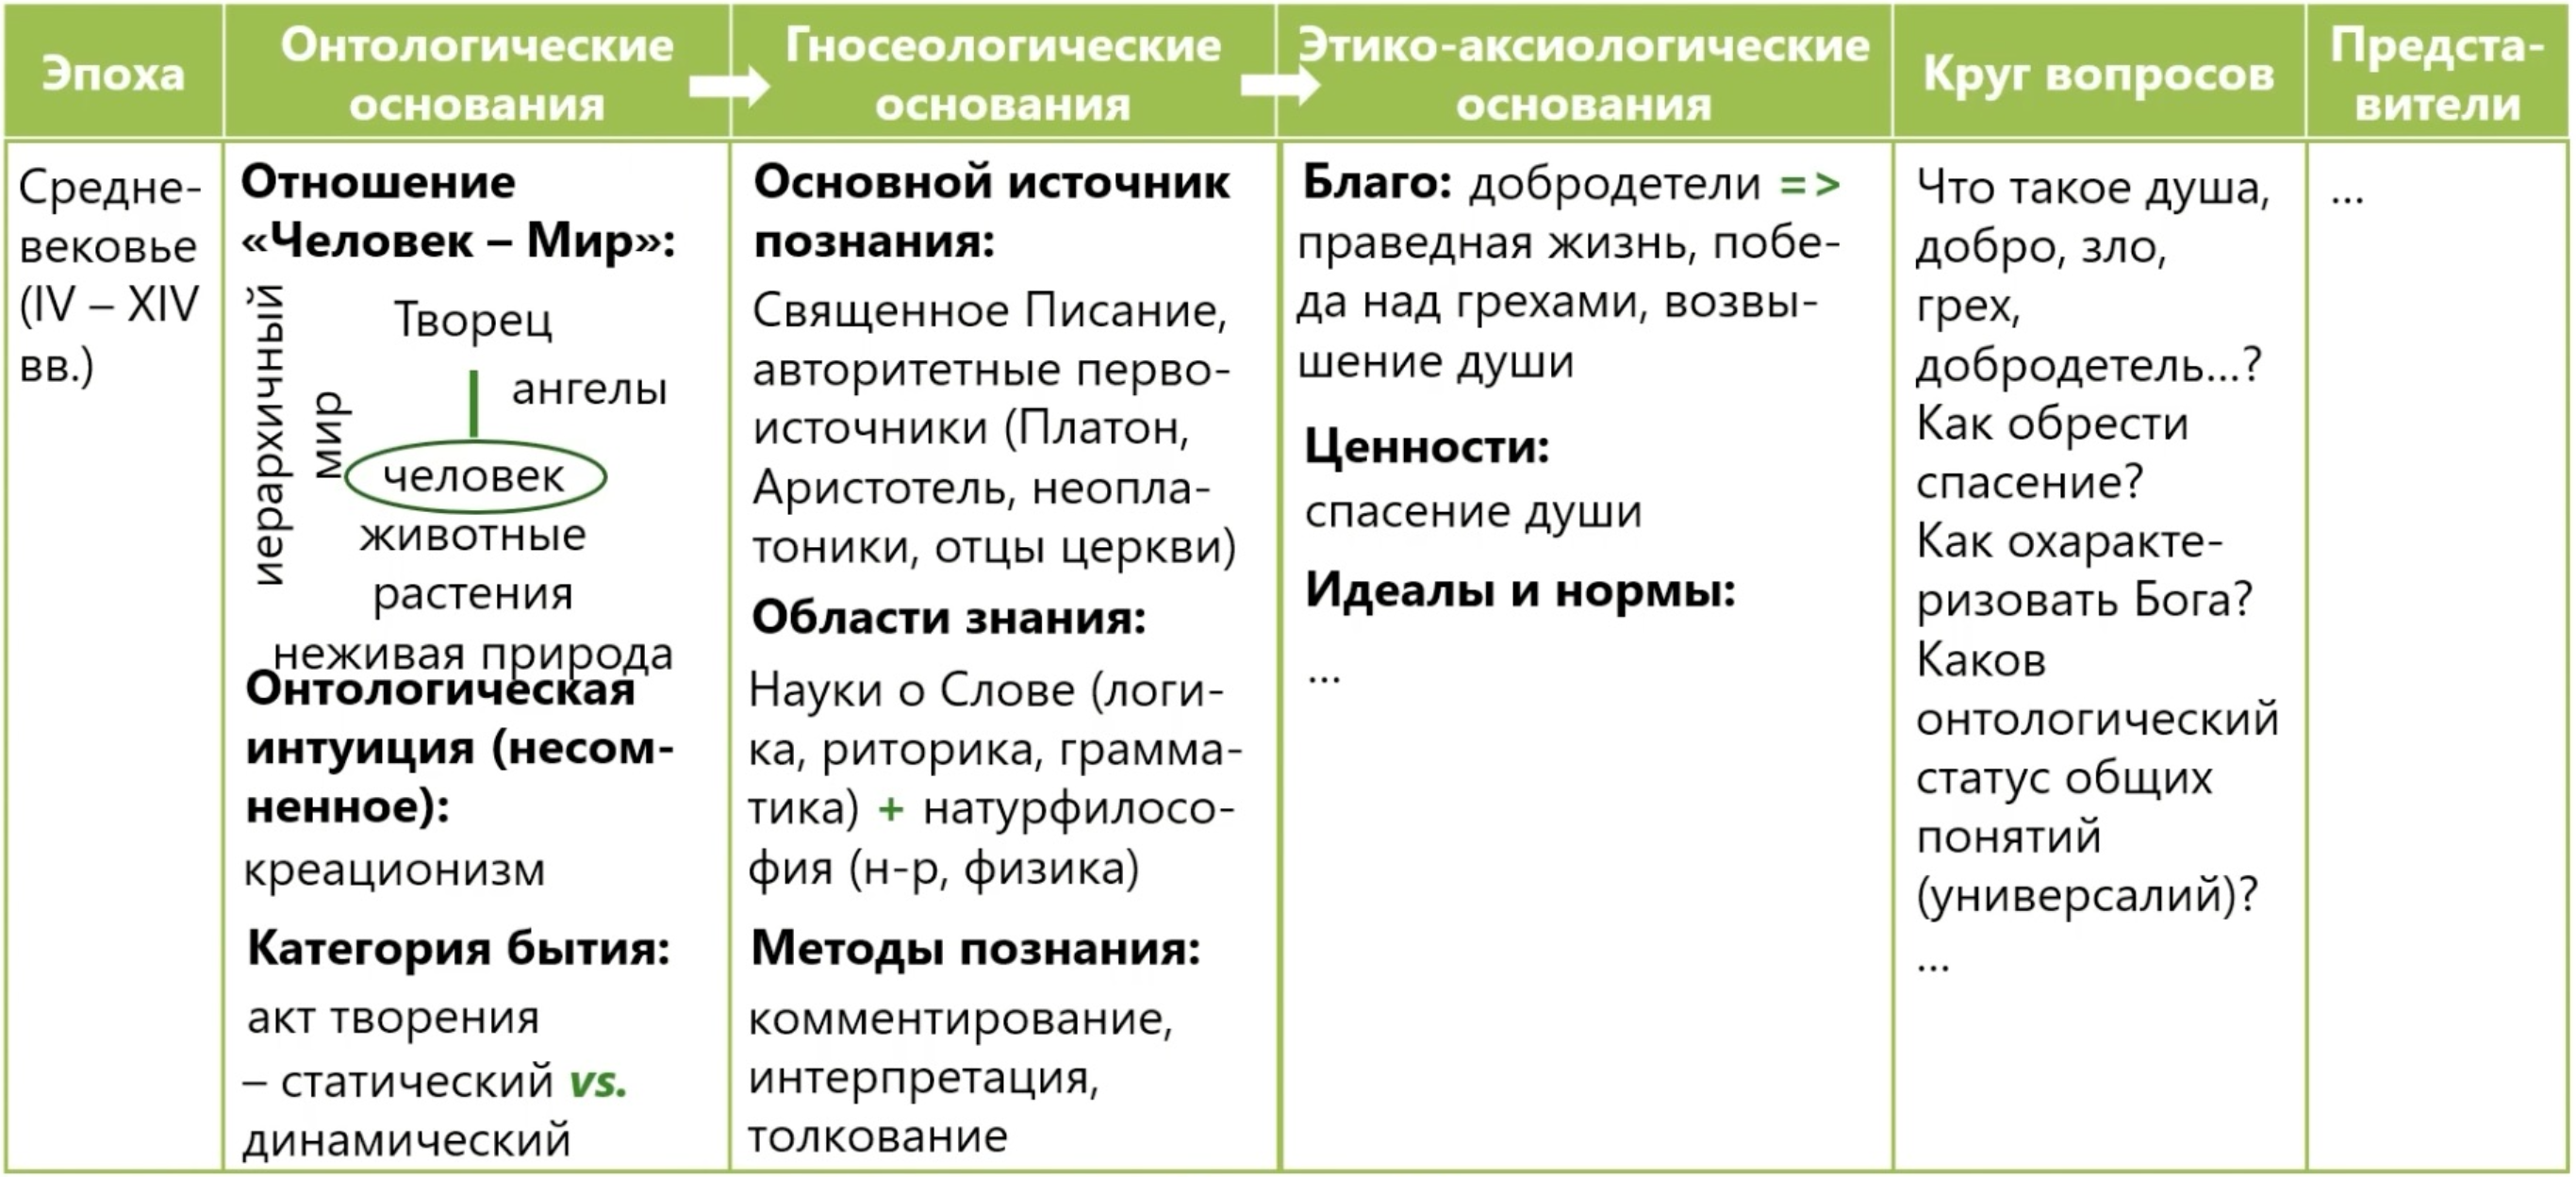
\includegraphics[width=0.8\linewidth]{pictures/med.png}
    \label{medieval}
\end{figure}

Гносеология изучает, как мы познаем. Познанию подлежит всё: от материалов до понятий вроде добра, от природы до Бога. Варианты познания различны, но это всё равно познание.

Эстетика интересуется прекрасным, которое можно увидеть, услышать, ощутить и выразить в разных формах.

Фундаментальные вопросы онтологии: как понимается отношение человек-мир, онтологическая интуиция, что такое бытие (В Средневековье: чистое бытие открывается в акте творения Богом, который создаёт каждую вещь; Бог — само бытие, сущность и существование тождественны; сотворённость мира Богом — очевидная истина.)

Мир Средневековья иерархичен: от неодушевленных камней до ангелов. Человек ниже ангелов, но обладает творческими способностями, будучи созданным по образу и подобию Бога. Мир эстетичен и статичен, но в нём есть динамика изменений.

Главная ценность Средневековья — Бог, а чистейшая часть человека — душа. Цель — спасение души, праведная жизнь. Основное обучение связано с интерпретацией Священного Писания и наставлением к праведной жизни. Познание природы второстепенно; преобладают методы комментирования текстов, авторитетными источниками служат труды Платона, Аристотеля, отцов церкви.

В Срнедневековье развиваются гуманитарные науки: грамматика, логика, риторика, герменевтика, экзегеза. Наука сосредоточена на слове; цитирование и аргументация становятся важными методами.

В античности мир воспринимался как единое целое, часть отражала целое. Например, кусок камня содержит свойства всего камня. В Новое время: целое состоит из частей, и части меньше целого. Декарт: понимание целого через анализ частей.

Каждая эпоха определяет культуру через философские основания. Отношение человека к миру влияет на жизненный уклад и способ познания. Эпохи трансформируются медленно, через накопление критической массы людей с новыми основаниями.

Наука развивается через смену концепций, но истина остаётся неизменной. Видение истины зависит от типа культуры (например, закон всемирного тяготения Ньютона --- истина существовала всегда, но была осознана лишь в XVII веке).

Понимание культуры невозможно без философских оснований. Исторические эпохи характеризуются различными способами познания, что связано с основными мировоззренческими принципами.

\subsection{Историческая проблема «начала» науки и деление на эпохи}

Задаваясь историческим вопросом <<в какой момент возникла наука?>>, прежде
необходимо определить, что понимается под наукой.

% с тем, на возникновение чего мы собираемся искать.
% Интересно, что философия науки, призванная заниматься осмыслением феномена науки
% в его бытийной и познавательной укорененности относительно молодая область
% исследований, начала выделяться в самостоятельную дисциплину, она лишь во второй
% половине XIX века с остановлением позитивизма, а прочное место в ряду
% университетских курсов заняла девушка к середине XX столетия. Такое позднее
% формирование отдельной философской области, посвященное специальному
% исследованию науки, наводит на мысль о недавнем по сравнению с искусством,
% религией, философией возникновении самой науки как специфического феномена,
% привлекающего к себе внимание лишь с недавних пор. 

% Задаваясь вопросом о том,
% когда наука стала такой, какой мы ее сегодня видим, с ее математизацией,
% экспериментальностью, небывалым размахом в плане масштабов внедрения во все
% сферы жизни и деятельности человека, 

Понимая науку как экспериментально-математический способ рационального познания мира, 
мы неизбежно упираемся в основание новоевропейской науки (рубеж XVI-XVII веков). 

% И достаточно распространена в современных исследованиях
% позиция, согласно которой науку считают самостоятельным видом деятельности,
% начиная с рубежа , в силу установления математики в качестве
% фундаментального языка описания природы и эксперимента в качестве ведущего
% метода познания. 
% В результате, отталкиваясь от данных, основополагающих
% концепции, большинство философов науки XX-го столетия обосновывает ,
% то есть науки в новоевропейском смысле. Этот смысл имеет и английская science.
% Как указывают исследователи, с одной стороны, до Галилея и Бекона не
% существовало экспериментов в собственном смысле слова, а с другой, наука,
% предполагающая царство рациональности, становится методологически строгой и
% математически точной, начиная с философии Декарта, положившей именно разум и
% рационально-логические законы пользования им в основании отношения человека к
% мир. Однако, понимание науки как феномена берущего начало в Европе в новое время
% и развернувшегося в XIX-XX веках в тот социальный институт, который сегодня
% повсеместно господствует, ставит обоснованный вопрос о европоцентризме или
% западном происхождении науки как таковой. Представители иных культур, в
% частности мусульманской, вполне закономерно возражают, что те неотъемлемые
% элементы, за которыми современная западная культура склонна видеть свое
% первенство, возникли задолго до XVII века в различных культурно-исторических
% локальностях. Так, например, математика с счетом геометрическими формами,
% которые одинаково для любого сознания человек пользовался по всей видимости
% столько, сколько существует человечество. В Древнем Египте и Мисопотами за 6-4
% тысяч лет до нашей эры на высоком уровне Личили, к примеру, было известно
% процедирование зубов. Были развиты математика, астрономия, фармацевтика, химия,
% сельскохозяйственная наука. В Древнем Китае, помимо остальных известных
% достижений, порох был изобретен не без экспериментирования, как минимум за
% тысячелетия до того, как через ближний восточных алхимиков его рецепты попали в
% Европу и начали активно применяться для изготовления оружия. Арабскими
% исследователями в области математики, алхимии, медицины, экономики и так далее
% многое было открыто и научно описано в 7-13 веках, то есть надолго до
% становления научной профессиональности в Европе. Существование на американских
% континентах до прихода европейцев, мощнейших империй, майя, ацтеков, инков
% невозможно представить без развития у данных народов всесторонней системы знаний
% от математики и астрономии до градостроения или лингвистики, чего стоит хотя бы
% узелковое письмо кипу и скоростная система передач информации инков, загадку
% которой до сих пор не удается понять современным исследователям. Подобные
% исторические факты о научных знаниях и технических достижениях различных

В попытке избежать европоцентризм, многие современные исследователи, задались
вопросом о науке как о феномене человеческой культуры вообще. Наука понимается как вид человеческой деятельности, которая состоит в построении системы знаний о мире. Тогда наука возникла с \textit{появлением человека}, который задолго до изобретения письменности уже
формировал картину мира, познавал и плоды своего познания применял в практических целях.

% И в разных культурно-исторических
% локальностях эти знания могут переплетаться с мистикой, магией, мифологическими
% объяснениями, философскими учениями, религиозными, догнами и так далее. Если мы
% таким широким образом понимаем науку как систему знаний и познания вообще, тогда
% ответ на вопрос о том, когда возникла наука, совпадает с ответом на вопрос о
% том, когда появился человек, который задолго до изобретения письменности уже
% формировал картину мира, познавал и плоды своего познания применял в
% практических целях. Однако, несмотря на свой методологический потенциал и
% предоставляемую возможность рассматривать науку как феномен культуры,
% обозначенная трактовка проигрывает рационалистическому пониманию в плане
% единства и четкости. 

% Невозможно, например, в рамках данного подхода решить
% проблему демаркации научного и ненаучного. Поскольку каждая культура
% вырабатывает свои нормы определения истинности знания, формирует свои методы
% соответствующие формы познания, институционализирует познавательную активность
% свойственные структуры и так далее, знания и познания любой культуры, даже
% далекие от традиционного понимания научности, тогда следует считать наравне с
% иными либо равноправными научными, либо равноправными ненаучными. Наконец, есть
% средний вариант трактовки науки и отчета ее начала, который мы будем далее
% использовать в нашем курсе. Если не любое знание можно охарактеризовать как
% научное, следовательно, не любое познавание окажется наукой. При этом, с другой
% стороны, под вопрос попадает обязательность экспериментирования, математизации,
% объективизации, как неотъемлемых свойств науки. Например, филологии,
% культурологии, истории и другим социумгументарным наукам представляется
% неправомерным отказывать в научности на основании отсутствия математического
% аппарата, экспериментальности и объективности, без чего же наука невозможна.
% Отвечая на этот вопрос, всматриваясь в самое существо науки в своем тексте под
% названием «Нука и осмысление», 

Мартин Хайдеггер определяет науку как теорию действительного. То
есть создание уме, представление, картины реальности, действительного, которое
выражается в научном знании.  Научное знание и методы его добычи впервые четко отделились от ненаучного
мнения как общепринятого суждения в Древней Греции (VII-VI вв. до н.э.)

% Такое определение науки коренится в слове
% древнегреческого происхождения, феория, открывая античный смысл, который можно
% подобраться в нашем языке к отражающему суть синамичному выражению, мысленное
% созерцание. То есть обязательное представление в голове обобщенных
% закономерностей и понимание их причин, а не просто совокупность разрозненных
% знаний или необязательно с математизацией и экспериментированием. Если теория
% отсутствует в основании науки, то математические выкладки останутся пустой
% абстракцией. Эксперимент будет безосновательным, новым совершаемым, поэтому уже,
% срок говоря, экспериментов не будет. Объективные закономерности рассыплются на
% нестыкуемые друг с другом осколки частных представлений. Понимание науки как
% теории действительного, как особого вида познания, которое невозможно без
% специального обращения к теоретическому уровню, позволяет также очертить границы
% науки как специфического вида человеческой деятельности, отделив его от иных
% родов человеческой практики. Древнегреческая философия в ее связи с наукой
% формируется в античности, отделяясь от мифологических объяснений, когда в русле
% менталитета и бытийных интуиций эллинов сложилось понимание необходимости и
% полезности специального практикования усилия мысленного созерцания. 

% Тогда же
% научное знание и методы его добычи впервые четко отделились от ненаучного
% мнения, как общепринятого суждения, которое в греческом называется докса, и от
% чисто практической деятельности, не подкрепленной теоретическим знанием причин.
% Поэтому, безусловно, на таком основании наряду с новым и новейшим временем
% нельзя отказать ни античности, ни средневековью, ни возрождению, как западным
% культурно-эстетическим эпохам в обладании в каждом конкретном случае особым
% собственным типом науки. Но, с другой стороны, развитие теоретической
% составляющей и выделение на данном основании научного познания в рамки
% социальных институтов, научных школ, сообществ, духовных практиков, отделов,
% перформных исследователей, жильцов и так далее дает надежные критерии для
% признания существования науки за пределами западной культурной локальности. Но,
% поскольку в нашем курсе мы именно ею вынуждены пока ограничиться, здесь и далее
% о науке будем говорить как о теории действительного, выделившейся в
% специфическую область деятельности в Древней Греции в 7-6 веках до нашей эры.

\subsubsection{Разделение культурно-исторических эпох в отечественной традиции}

Историю науки делят на два кардинально различающихся крупных периода: \textbf{натурфилософский этап} развития науки (эпоха Античности, Средневековье и эпоха Возрождения) и этап \textbf{научной рациональности}(XVI-XVII вв.: Классическая, Неклассическая и Постклассическая рациональности).


\subsubsection{Разделение культурно-исторических эпох в западной традиции}

Выделяется период Модерна (рубеж XIX-XX вв.) --- отказ от абсолюта, от
Бога, от принятых устоев, традиций, ценностей, от необходимости единого,
устойчивого в культуре в целом и в науке в
частности.

Домодерновый и Постмодерновый периоды выделяются естественным образом.

\chapter{Натурфилософские программы античности I}
 лекции по истории и философии науки. Сегодня мы переходим к самому объемному
разделу нашей дисциплины, который называется «История науки в ее связи с
философией». И здесь, прежде чем начать пятую тему, нам надо затронуть один
важный для понимания целей нашего курса вопрос. Зачем мы занимаемся историей
науки? Почему нам недостаточно познакомиться лишь с современными представлениями
о методологии исследовательской деятельности и ее социальной организации? Это
нужно, чтобы понимать, чем мы занимаемся, когда занимаемся наукой. Сможем ли мы
по-настоящему заниматься наукой, если для нас она будет чем-то не вполне
знакомым? Как можно спросить, сможем ли мы по-настоящему понимать человека, если
толком не знакомы с ним? Мы вроде работаем бок о бок каждый день, знаем его имя,
как он выглядит и так далее, но совершенно не представляем, как с ним быть, чего
от него ожидать, как выстраивать коммуникацию. Точно так же, как про интересного
нам человека, мы хотим знать что-то о его прошлом, причем не просто факты, там-
то тогда-то родился, он столько-то пошел в школу, ходил в какую-то секцию, то мы
хотим узнать о его переживаниях, о его детских воспоминаниях, о его друзьях, его
страхах, кризисах, их преодолении, словом о том, как он формировался, на
основании чего принимал судьбоносные решения и каким образом поступал в сложных
ситуациях. Тогда и информация о датах, цифрах, именах не так важна для понимания
человека. А, собственно, что важно? Важны условия, в которых он рос и
воспитывался, и важны его собственные основания, ориентиры, которыми он
руководствовался в прошлом и руководствуется сейчас. Тогда только мы можем
действительно понять человека и сказать, что это близкий человек, с которым нам
интересно и которому мы готовы уделять много времени, когда мы понимаем
основания его суждений, поступков, выводов. Примерно то же самое имеет место в
случае, когда мы хотим близкого знакомства с делом нашей жизни, буквально с тем,
чему мы посвящаем огромную часть своего времени. Наука не всегда была такой,
какая она предстает сегодня перед нами. Более того, она и сейчас
трансформируется, изобретает новые методы, совершает революционные открытия и
сталкивается с новыми проблемами. Она живет. А понять живое существо в том числе
значит узнать о том, как оно развивалось, на каких основаниях действовало
раньше, на каких и почему действует сейчас. История, лишь по видимости
дисциплина о прошлом, это исследование настоящего в его временной глубине. То,
что здесь и сейчас, не было бы таковым без своей истории, если не только что
возникло. Мы поэтому должны смотреть глубже и организовать наши исследования,
иначе, чем историографическая маркировка тех или иных вех на пути трансформации
научного знания, научной методологии. Сами по себе даты, названия, имена, лишь
точки или пунктирные линии, которыми мы размечаем пространство истории науки. Но
само это пространство не только из них состоит. Оно соткано смыслами. Чтобы
раскрыть для себя эти смыслы, мы должны смотреть глубже и стараться понять
основания того или иного исторического этапа, той или иной культуры, эпохи. Мы
должны научиться у истории науки ставить вопросы и изобретать способы их
решения, вдохновляясь теми проблемами, традицией их обсуждения и ходами мысли,
которые уже до нас и для нас разрабатывали предшественники. Таким образом,
научаясь о истории, мы, самое главное, сможем уверенно выйти к своим основаниям,
которые представляют собой единственный надежный фундамент для наших собственных
суждений, теории и способов поступать. Когда ставится вопрос об основаниях
представлений той или иной эпохи или типа науки, это вопрос о способе
миропонимания, о философских основаниях соответствующего типа культуры. И дело
не только в том, что философия формирует понимание отношений человека к миру,
отталкиваясь от которого каждая отдельная наука углубляется в исследование своей
области реальности. Когда-то между философией и наукой вообще невозможно было
провести границу, они были единым целым. Геометрическими формами обозначались
первоосновы всего сущего, а исследование природы было предметом глубочайших
философских изысканий. Медицинские практики ориентировались на движение небесных
сфер, а бытие описывалось в математических понятиях. Имя этому этапу жизни науки
в её связи с философией — античность. С данной культурно-исторической эпохи мы
начинаем отчёт науки и философии в их совместном становлении в европейской
традиции. Пятая тема курса носит название философской школы «Натурфилософские
программы античности». В рамках данной темы нам предстоит, внимание, две недели
занятий. Античность у нас единственная, занимает на лекциях четыре пары, все
остальные эпохи будут по две. Мы так сделали в нашем курсе, чтобы достаточно
времени уделить самой базовой эпохе, от которой отталкивается вся последующая
европейская философия и наука. Так что разберём четыре экзаменационных вопроса,
к первому из которых мы сейчас перейдём. Второй рассмотрим на второй паре
сегодня, а третий и четвёртый пойдут у нас через неделю на следующем занятии.
Итак, первый вопрос в пятой теме звучит следующим образом. Социально-культурные
условия формирования античной философии и науки. Почему такая именно у нас
логика будет раскрытие вопроса? Мы будем двигаться по нашей схеме изучения
культурно-исторических эпох, который мы разобрали в третьем вопросе предыдущей
темы, перевёрнутая пирамида. Помните, сначала набираем контекст, пишем
социокультурную ситуацию в Древней Греции, времён выделения науки и философии в
специфические виды деятельности. Из этих исторических моментов затем мы
стараемся вывести базовые принципы всего античного мировоззрения и по такому
пути выйдем к фундаментальным основаниям эпохи, антологическим. Так, поняв эти
основания, мы получим ключ, отпирающий дверь к действительному пониманию
философских идей и научных изысканий данного культурно-исторического периода.
Теперь спросим, зачем. В античной философии свёрнута вся последующая философия,
в античной науке свёрнута вся последующая наука. В этот период каким-то чудом
сформировался наш способ мыслить, и какой бы далёкой ни казалось эта эпоха, на
самом деле она в нас сегодняшних глубочайшим образом укоренена. Следовательно,
открывается поразительная перспектива. Изучая основания античного мышления, мы
параллельно сможем прояснить что-то и в своих собственных основаниях, и в
устройстве своего собственного способа мыслить. Итак, начнём с поверхностных
слоёв культуры. Первонаперво нам нужно воссоздать её контекст. Что мы уже знаем
об античности со школы сроков истории и МХК? Припомните, пожалуйста, какие в
целом у вас формировались ассоциации с словом античность. Давайте
последовательно будем отмечать самое общее. Локализуются истоки античной
культуры в Древней Греции, а затем в Древнем Риме. Чётко выделить временные
рамки этой эпохи тяжело. Существует множество вариантов отсчёта, каждый из
которых имеет веские доводы в свою защиту. С начала античной эпохи мы в нашем
курсе условно обозначим с XI века до н.э. С этого момента берёт начало так
называемый Гомеровский период античной истории. Идёт активное формирование
культурной традиции. В своих постоянных чертах оформляются мифы и легенды о
богах и героях. Появляются литературные произведения, посвящённые в частности
странствиям Одиссея и Триянской войне. Это события примерно XIII-XII веков до
н.э. Также с XI столетия до н.э. происходит формирование древнегреческих
полисов, городов-государств, представлявших собой специфические административные
образования, взаимоотношения внутри которых и между которыми также легли в
основании социокультурных особенностей эпохи. Окончание античности тоже
датировать непросто. Обычно отсчёт следующей эпохи Средневековья начинает с
упадка Римской империи, имевшего место в IV-V веках уже н.э. Хотя, например,
величайший философ раннего Средневековья, один из отцов церкви, святой Августин,
жил и творил свои произведения до окончания распада Римской империи, его годы
жизни 354-430 годы. В общем, будем иметь в виду условность такой датировки. На
сегодняшней лекции в плане развития философии Нуки нас будет больше всего
интересовать Древняя Греция, в которой в VII-VI веках до н.э. эти формы
культурной деятельности человека выделили специальную сферу занятий. Римской
традиции первых веков н.э. мы обязательно коснёмся во второй половине занятия на
следующей неделе. Что касается географии, древнегреческой культуры, племена
единого этнического происхождения населяли достаточно обширные территории
Средиземноморского и Черноморского побережья. Древняя Греция или Эллада в те
времена не представляла собой единого государства в той форме, в какой
национальные государства существуют сейчас. Тогда не существовало привычных
межгосударственных границ, а поскольку каждый крупный населённый пункт, полис от
греческого поли, много, но если множество людей, имел в своей власти систему
управления, то фактически по своему статусу представлял собой город-государство.
Тогда сформировались политические отношения, тоже от слова полис, отношения
людей по поводу их совместного проживания, регулирования дел этого сообщества,
внутренней власти и системы управления. Межгосударственные отношения были
буквально межполитическими, то есть выстраивались между полисами. И нередко за
счёт развития дипломатии организовывались союзы таких городов, как для ведения
междоусобных разборок, так и для противостояния внешним врагам, к примеру,
персам, стычки с которыми насушенные на море не были редкостью. Внимательно
посмотрите на карту колоний Древней Греции. Эллины имели колонии в Малой Азии на
территории современной Турции, проникли на восток вплоть до полуострова Крым в
Чёрном море, оставив там знаменитый Херсонес, колонизировали Черноморское
побережье современного Краснодарского края, а также прибрежные земли на
территории современной Грузии. Западные древнегреческие колонизаторы населяли
Сицирию, некоторые территории современной материковой Италии, побережье Испании
и множество островов, окружающих современную Грецию. В рамках этой темы мы будем
обсуждать философские школы, основанные в таких разнообразных местах, как Милет
в Ионии на территории современной Турции, Картон и Элея в современной Южной
Италии, Афины, современная столица Греции и так далее. Как раз на современной
карте я отметила некоторые полюсы, культурные и экономические центры Древней
Греции, в частности гору Олимп, на которой, согласно мифологии, жили боги. Таким
образом, даже уже бросив взгляд на карту, мы можем сделать вывод о том, что
древние греки были отличными мореплавателями и путешественниками, активно
исследовали новые земли, выстраивая с ними экономические и культурные связи за
счет обмена товарами и взаимного обучения. Развитие мореплавания обусловлено
благодатными географическими и климатическими условиями побережья материковой
Греции, изрезано бухтами и заливами вокруг множества мелких и крупных островов,
отсутствуют неблагоприятные морские течения и экстремальные погодные условия. В
полюсах процветали различные ремесла, торговля, занятия искусствами. На обширных
плодородных почвах Средиземного моря развивался седлое земледелие и
скотоводство. Развитие ремесел, искусств в соединении с активным мореплаванием и
колонизацией позволили мощнейшим образом укрепить экономику Древней Греции. За
счет открытия морских путей сообщений появились как восточные, так и в западные
рынки сбыта производимой сельскохозяйственной и ремесленной продукции, а также
предметов роскоши. Надо сказать, что понятие колонизации в случае с древними
греками необходимо отличать от современных наших представлений об этом феномене.
Поскольку в то время не существовало как таковой границ национальных государств
и не было понятия суверенитета, многие земли оставались просто неосвоенными. И
вот на диких побережьях греки высаживались для более удобного осуществления
торговли с другими народами, основывая колонии. Этимологически это слово одного
происхождения с нашим культ культура и означает обработку, освоение. То есть
древнегреческая колонизация с расселением по таким обширным территориям не была
завоеванием чужих земель, а изначально предполагала постройку новых полисов на
неосвоенных землях для абсолютно мирного взаимодействия с другими народами. А к
другим культурам греки относились с огромным почтением, с удовольствием общаясь
с местными жителями, слушая их жизненные истории, знакомясь с их бытом и
мифологическими представлениями. Также и рабовладельческий строй, характерный
для античной Греции, нельзя, на мой взгляд, рассматривать лишь с отрицательной
стороны. Конечно, всякое бывало, и в реальном человеческом обществе во все
времена, независимо от уклада, к сожалению, жестокость неизбывна. Так что
негативные моменты нельзя привязывать ни к конкретной эпохе, ни к определенному
экономическому строю. Но про рабовладение часто говорят о негуманности,
неправильности принуждения и лишении человеческих прав и свобод. Это все верно с
нашей сегодняшней точки зрения. Но для древних греков оно было естественно
сложившейся и глубоко укорененной в культуре традицией, возникшей первоначально
преимущественно по принципу долгового рабства. Когда один человек не был в
состоянии вернуть другому одолженные средства, он даровал господину свою
свободу, становясь его рабом. На самом деле с рабами в ранней античности все
было не так печально, как нам думается. Они могли выкупить себя из рабства и со
временем получить гражданство, то есть обрести статус свободного члена полиса.
Нередкий случай, когда за определенные заслуги господин сам даровал рабу
свободу. Примечательно, что во многом именно благодаря рабовладению граждане
полиса смогли освободить себе время для обучения, развития наук и искусства,
также совершенствования системы государственного управления. Таким образом,
организовав свой быт путем профессионального разделения обязанностей, эллины
преуспели в различных видах деятельности, опережая многих соседей или достойно
соперничая с ними. Это дало не только, как мы бы сейчас сказали, техническое и
военное превосходство. Народ, настолько интересующийся, изобретающий и
совершенствующий формы культурного самовыражения самой своей деятельностью и
идеалами этой деятельности, завоевывал авторитет и внышал уважение. Что еще мы
знаем о культуре Древней Греции? Чем обусловлено ее единство и влияние на столь
обширных территориях? Во-первых, это, безусловно, язык. На древнегреческом
записывались мифы и легенды, создавались поэтические, эпические, драматические
произведения, далась переписка, описывались исторические события, хронология,
генеалогия знатных родов, математические расчеты и исследовательские наблюдения.
Причем желающие могли ознакомиться с этими записями, специально изучать их,
обучаться по книгам. То есть, в отличие от цивилизации, например, Древнего
Египта и Месопотамии, в культуре Древней Греции доступ к передаче знаний,
историческим документам и литературным произведениям имели не только избранный,
обычно узкий круг жрецов и семья проявителя, но все свободные граждане. Так
каждый, в том числе и свободные женщины, могли обучаться тому мастерству,
которое приходилось по душе, от математики до ораторского искусства, от
врачевания до военного дела. И затем уже в свои философские школы женщин будут
принимать наравне с мужчинами, например, Пифагор и Эпикур. Открытый доступ
общества к произведениям культуры в широком смысле к искусству, мифам, истории,
наукам, возможность путешествовать, обучаясь в разных местах и древнегреческий
язык, интегрирующий все эти формы деятельности, безусловно, обеспечивали бурное
развитие всех сфер культуры Древней Греции. Влияние древнегреческого языка на
другие языки, а следовательно и на другие европейские культуры колоссально. Вы
смотрите, я только что употребила слово колоссально, оно древнегреческого
происхождения означает гигантский по размеру. Наверняка вы слышали о колоссе
Родоско. Так даже в, казалось бы, далеком от Греции, нашем Отечестве, в
повседневном обиходе, используется огромное количество слов, происходящих от
древнегреческих корней. До сих пор в обыденной и художественной речи
используются фразеологические выражения, имеющие древнегреческое происхождение.
Даже само словосочетание «крылатые» выражения восходит к Гомеру. «Почивать на
лаврах», «Сизифов труд», «Яблоко раздора», «Петь дифирамбу», «Рок изобилия»,
«Ахиллесова пята», «Ящик пандоры» и так далее. В основном к нам эти отпечатки
древнегреческой культуры пришли через Византию, восточную часть Римской империи,
югром, которая была уже в более поздний период Греция. Возьмем первые попавшиеся
примеры в научном нашем языке, пожалуй, древнегреческих корней не меньше, чем в
обыденной русской речи. Например, «архе» с корнем «арх», обозначающим «древний»,
«главный», «очень». Отсюда «архаичный», «архитектор», «главный строитель». Еще
говорят, например, «архи сложный», значит «очень сложный». Далее. Наши атомы от
«атомос», что значит «неделимый». Наша теория от «феория» – мысленное созерцание
того же корня теорема. Логика, наука логика, с древнегреческого учения о
правильных суждениях или о правильном мышлении. Аризматике от «аритмос» или
«арифмос» в другой транскрипции. «Число», там же корень «ритм» или «рифм», что
является своеобразным языковым указанием на единство музыки со счетом числом.
Кстати, и «музыка» от «музике», что является однокоренным со словом «муза». Муза
– покровительница искусства наук, спутница бога Аполлона. В честь них искусство
в нашем современном смысле называли тогда «мусическими искусствами». А само
слово «искусство» техны понималось более широко, как вообще осмысленная
деятельность человека. Например, искусство землепарца, гончарное искусство,
искусство врачевания и подобное. Искусство как вида человеческой культурной
деятельности, а не в смысле того, что это выражение ощущений и переживаний по
произведению, и как мы сейчас понимаем искусство более узко. Наконец, «психе» –
это душа. Отсюда психология, наука о психике, о душе. Ну, такие примеры можно
приводить еще долго. Это интересное занятие. Вы попробуйте на досуге поискать
другие древнегреческие корни в словах нашего языка, особенно в ваших научных
областях, и почитайте об их происхождении и значении. В таких герменофтических
практиках также должно многое открыться для понимания глубинных истоков
современной науки. Идем дальше. Во-вторых, единство любой культуры
обеспечивается и единством мировоззрения. А что такое мировоззрение? Это то, как
люди видят мир, то есть какие у них представления о возникновении мира, его
структуре и законах, по которым он функционирует. Исторически первой формой
представления о мире является мифологическое объяснение его устройства. Оно
предполагает одушевленный характер всего мира, управления им чьей-то
могущественной волей и сверхчеловеческими способностями. Обычно в мифах также
предполагается хотя бы случавшийся ранее непосредственный контакт божеств или
божественных бессмертных существ с людьми, с миром смертных. Собственно, и мифы
Древней Греции, о которых у каждого из нас есть представления с детства, не
являются в этом плане исключением. Подробнее, мне кажется, о содержании
древнегреческих мифов сейчас нецелесообразно говорить, однако еще несколько
деталей стоит отметить. Самое важное здесь, на мой взгляд, то, что
мифологические представления удовлетворяли человеческую потребность в объяснении
окружающей действительности. Они давали ответы на вопросы о том, как произошел
мир, как он устроен, кем управляется, каким нормам и идеалам необходимо
соответствовать в собственной жизни. И до поры до времени этого мифологического
мировоззрения было достаточно, чтобы существовать и ориентироваться в мире.
Данные особенности мифологического мировосприятия вместе с вниманием древних
греков к языку не могли не отразиться в искусстве Эллады. Для почитания богов
строились величественные храмы из камня в связи с чем развивалась архитектура.
То есть принципы построения зданий используются не только для святилищ, но и для
иных монументальных построек. Снаружи и внутри храмы необходимо было украшать,
поэтому в силу распространения таких наиболее доступных материалов, как камень,
мрамор, глина, металл и сплавы, развитие получали в первую очередь пластические
искусства. Скульптура из камня и бронзы, огончарное мастерство, выкладывание
мозаик, техника росписи фресками и позже камнерезное искусство и,
соответственно, создание барельефа стали основными составляющими
древнегреческого изобразительного искусства. Изображались прежде всего
мифологические персонажи и события с их участием. С другой стороны, устная
передача мифов и легенз способствовала их значительному искажению. Каждый
рассказчик произвольно мог от себя добавлять те или иные детали, допускать
неточности, путать последовательность возникновения богов, в связи с этим со
временем появилась необходимость письменной фиксации взаимосвязи всех
божественных существ древнегреческой мифологии и восстраивания более или менее
единого и непротиворечивого мифологического объяснения мира. Поскольку дела
богов мыслились священными и возвышенными, лежали в основании миропонимания и
несли получающую воспитательную функцию, излагать мифы и легенды надлежала
наиболее высоким стилям в поэтической форме, соблюдении ритма и в сопровождении
музыкальных инструментов. Любовь эллинов к рассказыванию и слушанию историй, к
языку, к речи, ее гармоничному и музыкальному звучанию сыграли ведущую роль в
становлении как словесного творчества, так и музыкальных жанров. Постепенно
совершенствовались музыкальные инструменты и изобретались наиболее подходящие
для того или иного словесного жанра стихотворные ритмы и размеры. Поэты, среди
которых следует обязательно упомянуть Гомера и Лисиона, соревновались между
собой перед публикой выразительности языка, стройности своих сочинений и полноте
передачи в них всех легендарных мифических событий. Собственно, благодаря
сохранившимся фрагментам их произведений мы и имеем современное представление о
древнегреческих мифах и легендах. Распространенными развлечениями с древнейших
времен были также празднества в честь погов с фестивалями и опрядами.
Неотъемлемыми элементами праздников являлись театральные представления,
разыгрывающие поначалу события мифов и сказания о героях Лады, а затем и
драматические произведения с самостоятельным сюжетом, которые постепенно
выделились в отдельный жанр. Спектакли могли быть достаточно длительными, а их
итоги бурно обсуждались зрителями. Самый важный тут момент. Давайте примечанием
отметим, почему так популярны были древнегреческие трагедии, почему собирали
тысячи зрителей в амфитеатрах и на стадионах. Думаю о таких трагедиях, как,
например, Царь Эдип, Антигона, Аристея, все имеют представление. В основе сюжета
лежит социально-этическая опория или парадокс, принципиально неразрешимая
противоречие. Буквально опория означает непроходимость. Слово опора в нашем
языке того же корня, но альфа-приватчевым дает отрицание. То есть опория – это
отсутствие опоры, отсутствие прохода опоры. Так, сталкиваясь с ситуацией, в
которой, в принципе, что бы ты ни выбрал, не получится хорошо для всех, герой
попадает в состояние омехании. Прямой перевод омехании – беспомощность. Такое
состояние ступора, когда мы не можем. Не можем применить никакие механизмы или
техники решения. У нас их много, мы почти все можем, столько всего умеем. Но вот
для этически затруднительных ситуаций, принципиально, нет заранее готовых
решений. И каждый раз нам приходится в конкретике уникальных обстоятельств
сделать выбор на свой страх и риск. Кстати, мы с вами об этом говорили на
третьей теме. Так вот, совместное переживание этого состояния повязанности по
рукам и ногам в таких ситуациях, пронзительное понимание одновременного и
величия человека, и его конечности, смертности, и неумения превозмочь порог
смерти, играло в древнегреческом полисе, городе-государстве роль, простите за
жаргон, таких скреп, на которых держался гражданский дух этого удивительно
мужественного народа. А древние греки и потом римляне, известные своим боевым
духом, побеждали армии других народов численностью до десяти раз превышающей их
войско и лучше вооруженных. Так вот, почему с внешней точки зрения, например,
убийцы своих родителей, Эдип и Арест, все-таки герои? Потому что они мужественно
выдерживают распятие на этой опоре непроходимости, изгоняют в себе пороки, и
благодаря этим чудовищным испытаниям судьбы что-то важное для себя понимают,
оставаясь людьми. Они как бы своей стойкостью, вопреки судьбе и смерти, держат,
выражая словами Мандельштама, место человека во Вселенной. И когда несколько
тысячный коллектив свободных граждан захватывает это переживание, они страдают
вместе со своими героями и понимают, что настоящее человеческое держится только
усилием, стремлением к высшим идеалам и усилием противостояния порокам в себе,
изгнания из собственной души каждым царя Эдипа. Я не случайно здесь произношу
слово «изгнание», оно связано в античном полисе и с такой уникальной практикой,
как острокизм. Голосование, в ходе которого каждый член полиса на общем собрании
писал на черепке или того, кто, по его мнению, наиболее опасен для города, и
того, кто набирал наибольшее количество голосов и сгоняли на 10 лет, как
минимум. Вы понимаете, что этого, естественно, каждый гражданин опасался. Все в
таком небольшом городе друг друга знали и старались для соотечественников
показывать себя с лучшей стороны. Мужчины таким образом буквально соревновались
друг с другом в проявлении добродетелей. Практика острокизма побуждала вести
себя честно, мужественно, справедливо, сдержанно и рассудительно. И древние
греки очень дорожили согласием со своими согражданами в полисе, потому что,
безусловно, изгнание, о котором слухи и сплетни моментально разносятся по
соседним полисам, было страшным позором. А кроме того, потери связей со своими
друзьями и родными, потери своего социального статуса, своего дела и, по сути,
имущества. Очень продуктивная система поддержания порядка, согласитесь. Но
вернемся от нашего углубленного примечания к дальнейшим чертам древнегреческой
культуры, в которых также проявляется соревновательный дух. Богам посвящались,
помимо перов и театральных представлений, многочисленные спортивные состязания
различного уровня и масштаба, известнейшие из которых Олимпийские игры
проводятся в мире по сей день. Спортивные соревнования служили не только в
качестве развлечений и зрелищ, но также позволяли различным полисам
продемонстрировать друг перед другом силу, красоту и способности своих атлетов.
В целом, дух торжества, благородного состязания и возвышенно эстетического
отношения к действительности вдохновлял Эллинов на новые свершения и в силу
такого позитивного соперничества способствовал все большему совершенствованию
различных сфер культурной жизни. Зрелища и праздники, на которые тратились
огромнейшие государственные средства, несоизмеримые по своему объёму даже с
военными расходами, на долгие столетия стали единящим древнегреческое общество
культурным ядром. Как вы понимаете, в любой культурно-исторической локальности
возникает некоторая среда, через которую, как через медиум, каждый отдельный
человек приобщается ко всему своему социуму, чувствует себя его частью и
поддерживает с другими его членами актуальной связи. Таким же медиумом,
например, в средние века выступала церковь. Все члены европейского
средневекового общества в неё ходили, участвовали в обрядах и празднованиях, и
благодаря этому у них поддерживалось такое социокультурное коммуникативное
пространство единых смыслов, в котором рождались и передавались байки и
различные мнения, шутки и серьёзные идеи. Поэтому страшно было отлучение от
церкви. Это означало буквально обрубить для человека возможность общаться, все
его связи с другими людьми. Как если бы нашему современнику, но совсем
заблокировали доступ в интернет и возможность пользоваться мобильной связью, так
что он бы даже электронную почту не мог посмотреть, позвонить родным или
произвести электронную оплату. Вот для нас сегодняшних дома такой средой
являются коммуникативные, цифровые, мобильные системы интернета, особенно
соцсети, мессенджеры и различные платформы, предоставляющие видеоконтент,
возможность трансляции, комментирования, интерпретирования и передачи друг другу
новых актуальных сюжетов. В недавнем прошлом функцию такого медиума выполняли
средства массовой информации, а в нашей стране, в том числе, очень похожем на
древнегреческое общество образом, обязательные коллективные мероприятия вроде
государственных праздников с парадами, субботников и тех же культурных программ,
походов в кино, на концерты, в театр. Так вот, у древних греков подобной средой
тоже были массовые празднества, посещение спортивных и театральных зрелищ, а
также общение на главной площади города, на которой в полисах обычно
располагался рынок. Именно там в основном обсуждались какие-то новости и
политические решения, рождались и передавались мемы, шутки, спледни и так далее.
Кроме того, монархические формы правления архического периода постепенно
сменялись в полисах олигархическими, то есть власть не обязательно передавалась
по наследству. Надо отметить, что древнегреческие правители отнюдь не были
настолько богатыми и богоподобными, как, скажем, персидские или египетские цари,
в полисах власть держалась поэтому в руках сильных духом людей, мужественных,
способных всего себя и всю свою жизнь поставить на карту, рискнуть всем ради
благородного поступка, например, отправиться в совершенно дикие, неизведанные
земли и основать там колонию, организуя при этом своих сподвижников и стараясь
обеспечить для них достойные условия жизни и интересную работу. То есть ценились
прежде всего дела, поступки, а не материальные блага или изнеживающие удобства.
Полисы развивались эффективнее под предводительством Совета, учитывавшего
социально-этические потребности граждан, культурно-экономические и военные
преимущества. Во вновь создаваемых городах на колониальных землях к управлению
гражданскими делами приходили наиболее влиятельные люди, полководцы, стратеги,
знатные и наиболее рассудительные граждане. Они завоевывали у народа авторитет,
покровительство развитию земледелия, ремесел, искусство, торговля и образование,
а также не скупясь на всевозможные развлекательные мероприятия, призванные не
только угодить богам, но и сплотить из сообщества полиса разнообразие в досуг
его членов. Таким образом, к VII веку до н.э. на территориях Древней Греции
складываются уникальные по своей специфике социально-культурные условия,
способствовавшие выделению в отдельной практике особой формы понимания
действительности теоретического мышления. Когда говорят о возникновении
философии и науки в Древней Греции, надо понимать, почему это слово берут в
кавычки. Как мы обсуждали на предыдущих занятиях, вспоминайте, знание как
таковое существовало и передавалось в различные культуры задолго до VII
встаретия до н.э. В Древнем Египте, на Месопотамии и на Востоке, в Древней Индии
и в Древнем Китае известны феномены познания, накопления опыта и передачи
знания. Однако, если можно в этот период говорить о развитии науки, то это была
практическая деятельность, а знание было фактуальным, то есть знанием о фактах,
которые прекращались, прежде всего, в обыденной жизни для тех или иных
практических нужд. И даже, казалось бы, самая теоретическая наука, математика,
использовалась исключительно для применения на практике, для счета измерения
предметов, планирования земельных участков и строительства. Так что мы будем
говорить осторожнее, скорее о том, что феномен теоретического мышления отделился
в эпоху античности от эстетически-мифологического миропонимания. Для понимания
этого ключевого момента давайте, прежде всего, вспомним со второй темы нашего
курса особенности теоретического уровня осмысления. К нему относятся высокая
степень абстракции, необходимая для выделения сущностных повторяющихся черт в
эмпирическом многообразии явлений. Кроме того, если для практической
деятельности характерен непосредственный контакт с объектом, то теоретизирование
происходит именно в уме, не с помощью связи с предметом за счет органов чувств,
но мысленно, независимо от физического ощущения. Так что, когда говорят о
теоретическом мышлении античной культуры, надо понимать, что вовсе не имеют в
виду, что до этого люди не умели обобщать, выделять сущностные причины и явления
или оперировать теми же числами, как предельной абстракцией. Речь идет о том,
что свойственное самой природе человека теоретическое мышление просто не было
систематически развиваемо. Не было до определенного момента самим человеком
замечено как нечто специфическое, как способность, которую развивать необходимо.
Об этом не совсем корректно говорить о том, что наука и философия возникли в
античности и, как в некоторых учебниках пишут, родились из мифов. На самом деле
в Древней Греции к VII веку до н.э. сложился комплекс условий, в которых, во-
первых, мифологические представления не могли дать ответы на интересующие
человека вопросы не о том, как все устроено в мире и каким должен быть человек,
а о том, почему все именно так устроено и зачем человек должен и должен ли быть
таким, как его рисует миф. А во-вторых, культурная и социально-политическая
жизнь побуждала специально развивать и практиковать именно теоретические
способности. Пока вы записываете, я немного прокомментирую, как я вижу эту
ситуацию. На самом деле многие исследователи реконструируют в кавычках
возникновение науки и философии, как именно появление каких-то новых практик в
силу неспособности мифа, как самозамплательную систему отвечать на интересующие
вопросы. Сама формула от мифа к логосу принадлежит советскому антиковеду Тихарио
Харлампевичу Кисиде, греку по национальности, работавшему в институте философии
РАН в Москве. Также подобное понимание характерно для, например, Алексея
Федоровича Лосева, тоже очень известного отечественного мыслителя, исследователя
культуры в ее символическом и эстетическом измерениях. Ну и, например, уже
знакомый нам Мираб Константинович Мамардашвили говорит, что наука не появляется
из простого накопления техник, умений, но обязательно человеку должно стать что-
то непонятно. В мифе все объяснено, и непонятного нет, а проблемность — это уже
черта науки. Но я не совсем с этой трактовкой согласна, поскольку, по-честному,
не знаю, так ли это было, хотя вроде бы логично и обоснованно, что жили себе
столетиями, тысячелетиями люди, пользовались мифологическими представлениями для
ориентирования в мире и не особо задавались вопросами о том, почему все именно
так устроено. А потом такие «стоп, посмотрите, вот непонятно ведь все в мире на
самом деле». С одной стороны, обильная историческая, философская литература
подводит к такому варианту, и нет оснований не доверять нашему гигантам мысли.
Элементарные исторические факты отсчитывают первые, собственно, теоретические,
не художественные, не мифологические произведения с VII-VI веков до н.э. с
Фалесом, Милецкого, Пифагора, Гераклита, Эфесского, Парменида и т.д. Но обратите
внимание, произведения, письменные источники, а как же устная традиция, тем
более в отношении мифа. Поэтому, с другой стороны, мне кажется, не задавались бы
люди вопросами, миф был бы один раз и навсегда. А миф очень текучий, изменчив,
передающийся из уст усталу в слове каждого рассказчика претерпевал изменения,
добавление уточнения, накапливались подробности, развивались все новые витки
сюжетов о богах и героях. Не от того ли, что просто основным, в смысле
привычным, уже сложившимся, средством, инструментом ответа на вопросы был в то
время миф, который можно было трансформировать. Однако, чтобы эту устную
традицию как-то все-таки устаканить, древнегреческие поэты начали в XI-IX веках
до н.э. мифы и легенды записывать. Ведь буква письменного источника тверже
текучести устной речи. Это, по сути, ошибка. Сделать статичным текучее по своей
природе обеспечило настоящий прорыв, который историки и датируют событием в
кавычках возникновения философии. Но на самом деле люди и так уже давно устно
задавались предельными вопросами, пытались для себя что-то понять, удивлялись
чудесно продуманным мироустройству и красоте мира и человека, как и любой
современный человек, но просто не выделяли это занятие в отдельный вид
деятельности и не практиковали специально. В тех же поэмах Гомера уже растворена
вся древнегреческая философия. Большинство философских категорий, встречающихся
в текстах античных мыслителей, слова обыденного языка, которыми и так народ
испокон веков пользовался. Это наводит на мысль о том, что всё-таки, возможно,
философию, науку, теоретические понятия не изобрели и не ввели. Наблюдательные
греки в VII-VI веках до н.э. скорее заметили, обратили внимание на вопрошение и
осмысление как отдельный вид деятельности, наряду с ремеслом, торговлей,
искусством, военным делом и так далее. А в Древней Греции в этот момент
складывалась благоприятная социально-политическая ситуация для осознания
неполноты мифа уже после Гомера Гищода и других поэтов статичного и
зафиксированного явления способности отвечать на предельный вопрос. Давайте
тогда резюмируем всё, что мы тут выше наговорили про начало античной культуры и
уже на более глубоком уровне понимания систематизируем по пунктам эти уникальные
условия того периода в Элладе, которые и побудили греков именно
институционализировать теоретические занятия в качестве самостоятельных видов
культурной деятельности. Развитие искусств, как пластических, так и словесных,
позволило на высоком уровне выражать в письменных и устных формах мифологическое
понимание мира. Во многом этому развитию способствовало поощрение занятий
искусством, а также сложившийся в рамках самого мифотворчества соревновательный
дух. Поэты, скульпторы, атлеты, музыканты, актёры постоянно совершенствовали
свои умения и оттачивали навыки, состязаясь друг с другом. Свобода и
зрелищность, публичность, культура Древней Греции к этому обязывали. В
результате развития словесных речевых жанров активно начали использоваться
художественные приёмы, метафоры и сравнения. К постоянному сопоставлению
обязывала и творческая и соревновательная атмосфера. Как раз сравнение и
сопоставление являются одними из основных теоретических процедур, работающих со
сходствами и различиями. Безусловно, выделение сходств и различий требует
высокого уровня абстрагирования, то есть мысленного одновременного представления
нескольких вещей, событий или феноменов и выделения в них на фоне общего
особенного. Однако к сопоставлению побуждали, как представляются и другие
особенности развития древнегреческой культуры. В силу освоения мореходства и
международной торговли происходило активное знакомство с другими этносами и их
культурами, что побуждало задаваться вопросами о нерушимости устоев собственного
мировоззрения. Другие цивилизации формировались под влиянием других мифов,
соответственно, на иных землях царил свой, отличный от древнегреческого уклад,
формировалось искусство другого типа и распространялись иные представления о
возникновении мира, природе материи и месте человека во Вселенной. Традиции,
обычаи и мифологию других народов греки сравнивали со своими, как мы уже
отметили выше, уважительно относясь к иным культурам и с удовольствием
выслушивая их сказания и предания. Безусловно, тесное взаимодействие действие с
другими народами не пошатнуло мифологические основы древнегреческой культуры,
однако сказалось на широте кругозора эллинов и переосмыслении некоторых моментов
собственного привычного уклада и мировоззрения с учетом опыта других народов.
Полис в качестве специфической формы совместного бытия в древнегреческом
обществе также стимулировал развитие критического и теоретического мышления,
становление олигархических, а затем демократических режимов правления в полисах
постепенно приобщало свободных граждан к вопросам правления, вовлекая в
обсуждение дел полиса. То есть у горожан появилась обязанность помимо
собственных дел заниматься также государственной деятельностью. Общегражданские
собрания проводились на центральной рыночной площади города, которая называлась
Агура. Проводились голосования, направленные на принятие государственных
решений. Каждый при желании мог высказаться в ходе обсуждения вопросов,
касающихся законодательства, полиса, празднеств и других культурных мероприятий,
внутреннего управления, экономических проблем, войны и мира и так далее. Таким
образом, для участия в политической деятельности требовались особые личностные
качества, самостоятельность мышления, критический подход, умение рассуждать,
аргументировать свое мнение, владение ораторским мастерством. В совокупности с
открытым доступом к образованию, что мы тоже уже отмечали, потребность в таком
типе мышления в огромной степени способствовала развитию дисциплин, логики и
риторики, а затем и становлению философского подхода. Все эти условия в целом
дали, как мы бы сейчас сказали, синергетический эффект. То есть совместно
благотворно повлияли на интенсивное развитие рефлексивного и теоретического
мышления, чего в условиях других величайших цивилизаций того же исторического
периода не произошло. Абстрагирование, выделение общего, сравнение,
сопоставление осуществляется умозрительно, то есть не путем практических
манипуляций в мире, но способом воссоздания в своем уме общей формы для
сопоставленных вещей или явлений. Умозрение становится основой, античного
теоретического мышления как метод, с помощью которого можно проникнуть сквозь
видимость к истинной сути вещей. Для чего же был выделен и культивирован этот
специфический способ мыслить? Как мы уже проговорили, мифологическое объяснение
мира, догматическое, по своей сути, не могло объяснить абсолютно все. Человеку
свойственно задаваться вопросами и живая тяга к пониманию никогда не уложится ни
в один статичный конструкт, ни в какие жесткие рамки. Зафиксированная мифология
не давала ответов на многие интересующие человека вопросы. Например, о том, из
чего все состоит, на чем держится единство всего мироздания, что такое добро и
зло, справедливость, мужество, красота, как поступать в противоречивой ситуации,
когда закон велит одно, а сердце подсказывает иное, какова природа человеческой
души и так далее. Ни миф, ни искусство сами по себе ответить на подобные вопросы
были не способны. Однако, несмотря на свою неспособность давать ответы на такие
фундаментальные вопросы, миф и искусство, безусловно, свои собственные функции
выполняли. Поэтому древним грекам вовсе не обязательно было отказываться от
эстетического наслаждения посредством искусства или от мифологического
объяснения вопросов сотворения Вселенной, влияния на человеческие дела. Просто
возникла необходимость осмыслять ряд вопросов другими средствами, чем миф или
искусство. И вот мы с вами сейчас наконец-то подобрались к самым
фундаментальным, глубинным основаниям античной культуры, чтобы ввести
содержатель. Ее онтологические основания мы должны предельно обобщить черты
миропонимания древних греков, о которых сегодня вот уже долго так говорим.
Систематизируем особенности мышления и ценностные ориентиры, которые легли в
основании древнегреческой философии. Итак, фиксируем для себя быстренько. Можно
две колоночки записывать, как представлено на слайде. Любовь к рассказыванию
историй, отразившуюся в мифах, подчеркивала и стремление знать генеалогию, как
происхождение было, так и свою родословную. Отсюда со временем формируется
специальный интерес к поиску причинно-следственных связей и приводит это к тому,
что фундаментальной особенностью древнегреческого типа мышления становится его
рефлексивность, осмысление через последовательную постановку вопросов о
причинах. Древнему греку было интересно все, от новых земель до древних
преданий, от замысловатого движения звезд на небе до отражения окружающих
предметов в мельчайшей капельке воды. Это культура интереса и внимания ко всему,
поэтому в сознании не выстраивалась иерархия окружающих предметов. Не было
различия по степени значимости между всматриванием в ход далеких звезд и
рассматриванием рысинки на траве под ногами, между слушанием дивных сказаний о
богах и интересом к себе смертного человека. Один из лозунгов древнегреческой
мысли, сформулированный первыми философами постулируют все во всем. То есть
отражение одного и того же присутствия, одного и того же события, любого
масштаба, вещи различной величины. Отсюда фундаментальные представления
древнегреческих первых. Мыслили о том, что все, что мы видим, все, что в мире
встречаем, состоит из одного и того же. Следовательно, все во всем может
превращаться. Более того, превращается на наших глазах из куска мрамора в
прекрасную статую, из жидкой массы во вкусный хлеб, из умершего гнющего тела в
плодородный слой, а затем, значит, в нашу пищу, а пища преобразуется в движение
нашего тела и нашего ума и так далее. Все безгранично переходит во все,
поскольку все пронизано чем-то единым. Греки умели восхищаться совершенством и
устройством природы. Стараясь подражать природе в искусстве, они
совершенствовали формы выражения, стремясь к изображению некого законченного
целого. Несмотря на понимание того, что все в мире течет, все изменяется, греки
умели видеть единичность, целостность, воплощенность, полноты в каждой
уникальной вещи. Поэтому целостность и завершенность, ограниченность и
оформленность стали идеалом. Тогда понимание сущего происходило через видение
его границ, его формы, его единичности как завершенности и полноты. В связи с
этим для первых античных исследователей, для всей античной культуры единица не
была числом. В полном смысле слово единица была основой числового ряда, счета,
однако она ценностно превосходила другие числа, составляющиеся путем
суммирования единиц. Важен был предмет в его целостности как своеобразная
единица, которую все и мерили. Также и мир как слаженность целого виделся
упорядоченной самой большой единицей, но тоже единицей. Греки ценили
упорядоченную организацию целого в природе, поэтому в искусстве, а затем в
мышлении в целом. Главнейшими принципами стали гармония и соразмерность.
Ценность имеет целое в единстве своих, пусть и разнородных частей и мерилось все
это философски понятая целостная единица. С ней все соизмерялось точнейшим
образом от пропорции идеальной колонны для храма до разницы в тонах звуков для
благозвучного музыкального произведения. Гармонично упорядоченно двигались
небесные сферы, значит и человек должен стремиться уподобиться этой гармонии
упорядоченной мысли и организуя свою жизнь. Наконец мы готовы ответить на вопрос
об антологических основаниях античной культуры. Напомню, мы их выделяем три. Как
понимается отношение человек-мир, что мыслиться несомненно, и что значит быть в
рамках соответствующего типа мышления. мир представал античному взгляду как
упорядоченная гармонично организованная целая космос. Поскольку же все
отражается во всем, каждая единичность также является полноценным целым. Человек
понимался как микрокосм, то есть как воплощение того же самого порядка, просто
относительно Вселенной более маленького размера. Тогда и во всей человеческой
жизни должно быть стремление к вселенской упорядоченности и соразмерности. Сам
человек должен становиться идеалом совершенства себя как внешне, так и
внутренне. Занятия должны воплощать совершенство, неупорядоченность и
оформленность мышления, а также проговоренность такого мышления, что
обозначается многозначным словом логос, означающим в том числе речь, порядок.
Этическим ориентиром становится добродетель, арите, как неотъемлемое свойство
настоящего правильного разумного человека. Несомненно, для древних греков, не
ставящимся под вопрос, было то, что мы называем вслед за Анатолием Вариановичем
Ахутиным антологической интуицией единого. Для античного человека несомненно,
было то, что все едино. Хотя, обратите внимание, налицо в мире множество
отдельных предметов. здесь демонстрирует свое существо как раз теоретическое
мышление, способное сквозь практическую видимость отдельности и разнородности
умозрительно выявить скрытую от физических глаз связь всего со всем, единства
всего. Раз все едино, для античного мыслителя оказалось очевидным, что все
состоит из чего-то одного. Как бы тогда все могло превращаться во все, например,
как бы мы усваивали пищу, если бы фундаментальным образом не состояли с ней из
одного и того же. Поэтому, задаваясь вопросом о том, из чего все состоит, и
находя разные элогичные ответы первые древнегреческие философы, тем не менее,
были согласны друг с другом в том, что это должно быть что-то единое, одно
начало для всего. Пронизывающий всю Вселенную порядок Логоса не только
обеспечивал своим единством правильную устроенность всего космоса, но и
отражаясь в человеческом уме, как бы настраиваемым на одну волну со Вселенским
порядком, гарантировал человеку способность понимать этот порядок с помощью
разума исследовать законы упорядоченности и соразмерности всего в мире. Так что
этот принцип, замыкающий на себя античное мировосприятие, явился принципом,
легитимирующим саму возможность теоретического познания, что без сомнения важно
для научной мысли любой эпохи. Ведь, чтобы достоверно познавать, нужно
основываться на том, что наше знание не выдуманный плод воображения, но оно
глубинным образом обеспечено благодаря связи наших научных теорий с тем, как мир
устроен на самом деле, наших научных законов с тем, каков настоящий порядок
устройства Вселенной. Конечно, когда мы в следующих наших трех вопросах подробно
познакомимся с идеями античных исследователей, у вас возникнет представление о
плюрализме, то есть множественности направлений. Можно утверждать, что между
мыслителями не было согласия и единства в самых фундаментальных вопросах о
природе материи, первичном, этом же едином, о причинности и так далее.
Действительно, особенно в поздней античности позиции стоиков, пекурейцев и
неоплатоников были непримиримы, они даже демонстративно по-разному стригли
бороды, чтобы подчеркнуть свою принадлежность к тому или иному философскому
направлению. Не искусственно ли мы тогда обобщаем под знаменем единого с большой
буквы всех без разбора представителей античной культуры, тем более столь
длительной и политически неоднородной? Уже у первых атомистов и взявшего их идеи
эпикура в природе базовых начала два атома и пустота их разъединяющая, и у того
же плотина, главного неоплутоника, единая, не только уж единая, распадается на
троицу, проявляясь во Вселенной и также в качестве ума с большой буквы и в
качестве души мира. Вот я сама долгое время пользовалась как штампом этим вроде
бы удачным выражением интуиции единого. Но после тщательного знакомства с
множеством разнообразных первоисточников античных авторов поняла, что правильнее
говорить об интуиции логоса, а не единого. Безусловно, не будет ошибкой
говорить, да если мы сегодня задумаемся над этим, почувствуем очевидность этого,
чем-то единым всё разнородное в нашем мире и правда как-то удерживается вместе.
Душа и тело, например, коллективные, индивидуальные, естественные, искусственные
и так далее. Другое дело, что это непостижимо и почему-то мы упираемся всегда
как минимум вдвоицу, в парадокс, в пары противоположностей. Неприступное это
единое, но всё же даже сам логос логики нас приводит к этому положению. На чём-
то же всё это должно держаться, иначе противоположности схопнулись бы и ничего
бы не было. Так что давайте впредь будем говорить, во-первых, о вкусе античных
мыслителей, к парадоксам, противоположностям, несовместимостям, а во-вторых, о
том, что несомненным для них было именно единство логоса во всём. что можно
своим умом настроиться на понимание фундаментальных законов Вселенной и
человеческого общества, которые, тем не менее, всегда включают в себя
двигательный парадокс, опорю. Наконец, поскольку идеалом был космос, размеренный
и упорядоченный противоположность хаосу, быть в мышлении древнегреческого
человека, по-настоящему быть означало иметь форму, быть целым, завершённым, то
есть имеющим границы, умеренным и при этом соразмерным остальному порядку мира.
Категория меры имеет для понимания античного видения ключевую роль. В
действительности реально быть, быть действовать, значит иметь меру, внутреннюю и
внешнюю соразмерность. Идеал человека быть живой мерой, то есть каждый раз, в
каждой уникальной единичной ситуации как бы примеривать себя к ней, соизмерять
всё и действовать размеренно, умеренно, согласно определённому порядку, а не
имитаться хаотично, беспорядочно действуя и не делать ничего сверх меры. Ничего
сверх меры тоже одна из своеобразных формул древнегреческой культуры. Согласно
такому пониманию, теперь становится ясно, например, почему богатые представители
античного общества, обычно к тому же воскообразованные, одевались скромно, не
пытались чрезмерно украшать свой дом или просто копить свои богатства в виде
золота. Умеренность во всём означало искусство гармонично упорядочивать свою
жизнь, цель которой отнюдь не могла быть мысленна в накопительстве или наоборот
в безмерном расточительстве. Тогда и быть познанным в качестве предмета или
явления мира означало быть включённым в гармоничное целое миро, быть понятым в
качестве оформленного и при этом соразмерного с другими элемента. Всё
беспредельное, а естественно, древним грекам были знакомы математическая
бесконечность и представления о безмерном мыслились существующими лишь
возможности. Их можно было вообразить себе, представить. Однако, поскольку в
мире космосе мы не сталкиваемся с такими вещами, а наоборот наблюдаем
упорядоченность форм и конечность всего внутримирного, то всему беспредельному,
неоформленному, аморфному, безразмерному, неумерному и так далее, античный ум
отказывал в действительном, реальном бытии. То есть, смотрите, при всей
похожести современности на античность, особенно позднюю, что я постараюсь вам
показать на следующей неделе, основополагающим антологическим различием наших
эпох является прежде всего разное отношение к категориям возможного и
действительного. Сегодня нам очевидным и несомненным представляется, что
возможность больше действительности. Ведь мы можем новоображать кучу всего, что
может произойти, чего в реальности непосредственно здесь сейчас нет. И на
основании этого мы поступаем и выстраиваем свою жизнь сплошь и рядом. Например,
живой классик, итальянский современный философ Пауло Лаверно абсолютно верно
подмечает, что, скажем, принимая человека на работу, работодатель смотрит не на
то, что человек реально делает, а доверяет ему, что у того гипотетически есть
способности для выполнения возможных задач. В свою очередь, работодатель обещает
сотруднику тоже возможности карьерного роста и определенных премий или повышения
со временем заработной платы. На деле не факт, что все это оправдается, но мы
полагаемся на такие воображаемые возможности. В Древней Греции надо было на деле
показать свое мастерство, чтобы получить признание, уважение и элементарное
вознаграждение за работу, показать, что ты умеешь, что ты уже реально сделал,
будь то атлетические спортивные трюки или глиняные горшки, песни или лошадиный
упряжь. Мы же на каждом шагу думаем, что у нас много возможностей пойти учиться
туда-то или туда-то, стать тем-то или тем-то, с этим ли человеком сблизиться,
куда поехать отдыхать, какую одежду для кого-то в случае купить. А что на самом
деле, каков настоящий выбор в сфере дел, поступков в мире, а не в голове. И эти
наши воображаемые возможности с удовольствием подпитывают рекламу, пропаганда и
социальные стереотипы. Мы сегодня очень мало смотрим на то, что действительно
здесь, сейчас реально есть. Мало всматриваемся в то, какими мы сами на самом
деле от природы являемся, а не какими нас хотят видеть в этих воображаемых
стереотипах. И, к сожалению, немало людей проживают в жизни, лишь строя планы в
голове и представляя себе, что у них есть возможности. На деле же из-за этого
ничего не успевая по-хорошему воплотить. Так вот, греки видят не так. Они
напоминают нам, что действительно больше возможного. Все наши воображаемые
возможности лишь у нас в голове. Они не имеют воплощения в реальности. А что
реально? Что в мире по-настоящему? Вот это греков интересовало прежде всего.
Конечно, мы отметили, что они первые начали специально практиковать
теоретические занятия, которые как раз именно в нашем воображении целиком
происходят. Но, обратите внимание, для античных исследователей разум
воспринимался как инструмент. Инструмент осмысления действительности, а не в
качестве пространства идолов и мечтаний, которым мы отдаёмся в рабство вместо
жизни в реальности. Безусловно, у человека любой эпохи существует соблазн витать
в облаках и погрязнуть в мечтаниях, не замечая того, что на самом деле
происходит. Однако, сами антологические условия, внимание античности к
настоящему, подлинному, действительному, к природе, как она сама по себе есть и
к человеку, какие поступки он совершает перед лицом сообщества, побуждали, что
называется, заняться делом и воплощать, в том числе, прекрасные произведения
искусства в реальность. Это очень важный момент для понимания всей
древнегреческо-философской научной мысли, поэтому постарайтесь тщательно
запомнить такой ключ к эпохе, антологические основания древнегреческой культуры.
Перейдём теперь в завершение нашего первого вопроса, отталкиваясь от этих самых
фундаментальных оснований эпохи к гносеологическим, этическим и эстетическим.
Интересно здесь прежде всего то, что в античности они были фактически
неразличимы, перетекали друг в друга. Основным источником познания мыслился тот
самый логос, несомненно, антологический принцип, то, что через всё в мире течёт
и всё упорядочивает как в космосе, так и в человеке. Логос — многозначное
понятие. Давайте кратенько здесь раскроем спектр его смыслов и отметим его
логоносеологическое значение для античного способа познания. Во-первых, это
слово или речь. В этом смысле, например, название науки филологии происходит от
греческого «любовь к слову». Во-вторых, не теряя своего значения речи, логос,
как вводилось это понятие первыми древнегреческими философами, мыслился как
некий всеобщий порядок Вселенной, который пронизывает всё своим течением. Логос
и однокоренное с ним лего, как конструктор назван, собираю, означает упорядочно
конструировать. Слушающаяся этого единого порядка природа кампуса образовывает
своё бытие с всё пронизывающим течением космической речи, делающей мир
членораздельным, оформленным. В-третьих, под логосом понимается мысль или
упорядочно оформленное мышление, мышление в понятиях, что на современный манер
можно трактовать как научную теорию. С данным значением как раз коррелирует
название дисциплины логики, которая нацелена на обучение правильности
упорядоченности мыслей и суждения. Сегодня при выяснении темологии название
большинства научных дисциплин, заканчивающихся на логии, типа биология,
психология, геология и подобных, логос в соответствии с данным значением так тут
как учение, что соответствует в частности пифагорейскому оттенку понимания этого
слова. Так, обучение правильному мышлению, настройка своего ума на слышание,
видение, текущего через все единого порядка обеспечивало по мнению
древнегреческих исследователей подключение к логосу как бы программе, которой
запрограммирована вся вселенная. И тогда всматривайся, анализируй, схватывай
порядок и придешь к истинному знанию. Так что истинное знание это логично,
полученное путем умозрительного постижения действительности через рассуждение,
которое обязательно соотносится с тем, как все реально есть, как мир нам
является. Поэтому не удивляйтесь, когда мы начнем рассматривать воззрение разных
античных мыслителей. Они не согласуются друг с другом содержательно. Каждым
авторам предлагаются разные объяснения причин природных свойств материи. Один
будет утверждать, что первое вещество, из которого в разных модификациях
составляются вещи, имеет свойство жидкости, поскольку все течет, изменяется, да
и без влажной среды нет жизни. Другой будет показывать, что в основе всего
огонь, как энергия, которая все в разной степени наполняет своим действием. И
попробуйте на основании современной физики поспорить, что материя в пределе не
энергия. Третий выскажет предположение о том, что материя в пределе число. И все
вещества формируются как отражение комбинаций этих чисел, а главное
соразмерность, гармоничное отношение. И попробуйте, исходя из современных
квантовых представлений о химической связи, поспорить с тем, что соединение не
обязано своим существованием как раз гармоничной согласованности энергетических
уровней, на которых находятся электроны, и которые никак попало образуют связи,
а в строгой порядоченности по определенным квантовым числам. Ну и так далее. Все
эти объяснения реально логично выводятся из определенных основоположений,
которых в рамках своего учения каждый исследователь придерживался. И более того,
звучат равноубедительно даже для нас сегодняшних, хотя и на непривычном языке
выражено то, что мы в своих научных теориях сегодня знаем. Это происходит,
поскольку каждая такая концепция рационально схватывает в действительности то,
что на самом деле имеет место. Другое дело, что каждый схватывает что-то со
своего уникального угла зрения, как бы какую-то более близкую грань в изучаемом
и не может охватить абсолютно все многообразие, выразив в едином
непротиворечивом принципе. Так что конкуренция познавательных конструктов наших
теорий одного и того же это нормально в любое время и античность, несмотря на
стремление к единству и попыткам его схватить выразить, не исключение, а скорее
первая научная эпоха, которая задает такое правило многогранного рассмотрения. И
тут, ребята, до меня на новом уровне доходят идеи Артегии Гассета. Помните, на
прошлой теме я вам цитировала про неизменность истины и изменчивость нашего
знания на примере формулирования Ньютоном законов всемирного тяготения. У Ганса
Георга Гадемера, выдающегося современного разработчика философской герминевтики,
есть подобная идея об истории как истории переосмысления понятий. Мы тоже это
затрагивали на прошлой неделе по поводу разного смыслового наполнения
философских категорий в разной эпохе. И вот банальные вроде бы идеи, но я читаю
античные первоисточники и проводя параллели с современной наукой прямо
прочувствовала на каком-то качестве на новом уровне для себя. Реально, ребят,
смысл знания, прозрение человека в сущность мира, порядка вещей вообще не
меняется. Но язык устаревает, и каждому новому поколению приходится фактически
изобретать новый язык, более понятный, чем те записи прошлого и трактаты
древних. Переоткрывается постоянно одно и то же, потому что логично же,
фундаментально природа не поменялась. Вселенная та же человек, так же
биологически тысячелетия, десятки тысяч лет назад. Но понятая кем-то и
выраженная языком его культуры истина может быть непонятна другому, даже
соотечественнику, скажем, его внуку. Непонятно в силу как раз фиксированности в
каких-то формулировках, уже не работающих для сознания новых поколений в новых
условиях. Конечно, существует прогресс как знания, так и мысли, но некоторые
фундаментальные законы природы и существования человека остаются теми же. Мы
просто сквозь призму своих социокультурных условий переводим их каждый раз на
язык более понятных нам мировоззренческих оснований. Вот поэтому, ребята, мы
изучаем античных авторов. Они уже максимально разработали то мыслительное
пространство для науки и философии, в котором мы до сих пор движемся, из-за
границы которого вряд ли человек выйдет, по крайней мере, пока он человек. По
поводу преобладающих методов познания можно после этого нашего разговора уже
даже не комментировать. Мы только что проговорили о возможном и действительном
вонтологических основаниях. Вспомните теперь со второй темой, чем отличается
наблюдение от эксперимента и соотносите со следующим соображением. Поскольку для
нас современных важнее и больше кажется возможным, в нашей науке с нового
времени процветает эксперимент. В отличие от наблюдения, которое происходит в
естественных условиях, эксперимент создаётся в искусственных. То есть он нацелен
на раскрытие не того, как природа сама по себе естественного действительности
есть, а того, какой она может быть, как она может действовать. То есть цель
раскрытия потенции, возможностей, а не рассмотрения актуальной действительности,
как в наблюдении. Безусловно, каким бы эмпирическим методом мы не пользовались,
теоретическое осмысление будет лежать в основании и для античных исследователей
важно было рационально осмыслить наблюдаемое, сформулировать на логичных
основаниях красивые, предельно простые обобщённые законы, а не просто
зафиксировать описание происходящего, что и так испокон веков до них все делали.
Но самое главное, чтобы вы понимали, я выражу это фразой Анатолия Варьяновича
Ахутина, грекам показалось бы парадоксальным, если бы кто-нибудь решил изучать
естественное, то есть природу и естество неестественными методами. В общем-то,
тоже абсолютно логично. В природе ведь есть только то, что есть, и возникает то,
что возникает, так наблюдай хорошенько за действительностью и познаешь всё. Ведь
возможностей в реальности нет, могло бы быть иным, но не иное, вот такое, какое
есть. И зачем тогда забывать себе голову фантазиями, если мы вот в этом, именно
в таком действительном мире живём, а не в придуманном. Ну а для современных
людей это логические условия такие, что им легко впадать в проживание
ненастоящей жизни, то есть в ненастоящем воображаемом мире возможностей.
Наконец, в этом свете не менее естественно, что знание развивалось обо всём
подряд. Нет, наверное, такого феномена или такого объекта, которого бы не
коснулось этичное любопытство. Так что в эту эпоху было создано знание по всем
областям действительности, зародились практически все наши современные науки, от
физики до истории, от биологии до психологии. Особенностью же эпохи является то,
что не выстраивалась особая иерархия дисциплин, ни в философии, ни в сфере
научного познания, да и между философией и наукой граница не проводилась. Даже
попытавшийся аранжировать по степени значимости для человека дисциплины
Аристотель сам создал головокружительную по своему охвату систему знаний просто
обо всём и равно был захвачен как подробнейшим наблюдением за животными, так и
мысленным созерцанием первопричин всего сущего, как пониманием причин
метеорологических явлений вроде молнии и радуги, так и разбором устройства души.
То есть, можно, безусловно, говорить особенно про позднюю античность после
Аристотеля, что намечается ценностное превознесение метафизики, первой
философии, которая должна прояснять самые фундаментальные первоосновы всего, но
она важнее, поскольку более фундаментальная. И, как Аристотель говорит, без
понимания первых причин любое наше знание будет шатким и фрагментарным. И,
конечно, чтобы упорядоченно мыслить и не совершать ошибок в познании, неплохо
овладеть инструментарием логики. Однако, это просто вспомогательная, буквально,
инструментальная дисциплина. Остальные сферы исследования уже отталкиваются от
определенным образом выстроенной антологической базы, но на которой равна
строится как этика, так и физика, как медицина, так и политика. Что важнее из
этих наук? Вот для античных мыслителей было очевидно и несомненно, что все эти
области одинаково значимы и все их надо развивать. Это дает нам возможность, в
конце концов, плавно перечечь в этические основания и эстетические идеалы.
Принципы разумности, гармоничной упорядоченности, соразмерности, это
одновременно не только антологические принципы, но и этические и эстетические
идеалы. Страшное слово «калок аготия» обозначает одновременно эстетическую и
этическую добротность. Происходит от древнегреческого выражения «калос каи
аготос», буквально «прекрасный и хороший» или «красивый и добрый». Этот принцип
предполагает совместное обязательное сочетание в человеке физической красоты и
добродетельности натуры. То есть был даже такой стереотип, если человек некрасив
внешне, то, скорее всего, он не особо хорош по характеру. Например, Сократа
завистники порицали за его курносость. Это считалось у греков некрасивым, хотя,
на мой субъективный взгляд, вполне обычный, непротивный мужчина, тем более с
отменным здоровьем. Он специально закалялся и регулярно выполнял физические
упражнения, а в Пелопонесской войне принимал участие в качестве гоплита,
пехотинца с тяжелым вооружением, которое носить на себе и которым владеть было
дело исключительных по силе и выносливости воинов. Но своим обидчикам мыслитель
отвечал, что хотя и не подходит к общепринятым канонам красоты, он изо всех сил
старался воплотить в своей жизни, по крайней мере, идеал справедливости,
рассудительности, мужества, внимательности, добродушия и щедрости. Про
умеренность во всем, как принцип жизни, мы уже проговорили в антологических
словах, это, я думаю, тоже особо можно не комментировать. Имеется в виду, что
идеалом античного гражданина было просто при этом опрятно и гармонично
одеваться, не демонстрировать ни умеренность в расходе средств или питаний, а
также уделять внимание равно своему физическому и духовному развитию, чтобы во
всем была пропорциональность чувства, меры и соразмерности, также и эстетический
идеал, который можно, конечно, выразить как красота в простоте, гармонии и
естественности. Очень напоминает, кстати, японский принцип ваби-саби, который
тоже не только эстетический, но и имеет глубокий антологический смысл. Так что
в, казалось бы, совершенно разных и похожих друг на друга культурах мы находим
сходные фундаментальные общечеловеческие основания. Про этический рационализм мы
подробнее обсудим на следующей неделе, когда будем говорить о Сократе и Плутоне.
Но пускай он тут у вас тоже будет в философских основаниях, означает этот
принцип буквально следующий. Если я разумом, а рацию одно да не разум, понимаю,
что такое благо, добро, справедливость, то я принципиально не могу себе
позволить поступить злым или несправедливым образом. Обратите внимание, знание,
гносиологическая категория, неразрывно связано с поступком, а это уровень этики.
Таким образом, подытожим, для античного мышления не характерны разделения таких
областей, как антология, гносиология, этика и эстетика. Поскольку
фундаментальным образом в своей основе всё едино, то ум, красота и добротность
просто разные грани проявления одного бытия. Оно к нам и в каждом человеке
должно являться полнотой, только если всеми оттенками играет, когда человек и
тело своё совершенствует, упражняет, и душу развивает, и разум занимает важными
задачами, рассуждая логично, и поступает по справедливости, по совести. Всё
красиво и стройно. Но, ребят, напоследок примечанием обращу ваше внимание вот на
что. Чтобы у вас не создавались идеализированные впечатления об античности, мы
тут отметили именно идеалы, то есть то, к чему человек стремился. А как вы
догадываетесь, реальные люди сплошь и рядом далеки от идеала, поэтому, несмотря
на высокие этические и эстетические принципы, некорректно было бы превозносить
античность и думать, вот времена-то были, что, мол, все, как на подбор, умные,
добрые, красивые. Реальные античные люди, многие, естественно, как и наши
современники, поддавались соблазнам далеко, не все были симпатичны и
пропорционального телосложения, не всегда могли умерить свой пыл, гордыню,
злогу, нерезко поступали несправедливо и так далее, как и все обычные люди в
любую эпоху. Однако, безусловно, среди них, опять же, как и все времена, были
самые выдающиеся представители нашего рода, которые реально своей жизнью
пытались воплотить эти идеалы, и мы через перерыв начнем, наконец, знакомиться с
теми из великих эллинов, которые посвятили себя исследованиям. На этом завершим
первый вопрос, пятой темы. Всем спасибо огромнейшее за внимание. Если есть
вопросы, с удовольствием отвечу. А ребята, вы тут. Итак, систематизировав в
первом вопросе антологические основания принципа античного мировоззрения,
перейдем ко второму, который в нашем списке к экзамену носит название «Первые
натурфилософские учения античности». Вопрос этот тоже очень объемный, будет как
первый сегодняшний, хотя пунктов в нем мы больше выделяем, просто потому что
множество натурфилософских школ возникло, и понемногу в каждую надо заглянуть.
Чтобы рассматривать сами учения древнегреческих мыслителей, нам прежде всего
нужно разобраться с понятием натурфилософии, которое, к тому же, пригодится вам
в следующих темах. Затем мы должны будем понять, в чем специфика античных
натурфилософских учений, какой круг вопросов объединяет ранних греческих
мыслителей. Следите за заголовочками, как обычно, все пункты сейчас
последовательно разберем. Для начала разберем, что такое натурфилософия вообще.
Существуют две трактовки данного термина. Чаще всего под натурфилософии
понимается философия природы, буквально с латыни «натура природа», то есть это
целостное осмысление природы как общего понятия, через которое, возможно,
становится объяснение отдельных вещей и познание ее фундаментальных законов.
Данное определение предполагает, в частности, что познание природы и ее частей
происходит умозрительно, теоретически, философски, в том смысле, что знание о
природе начинается не с практического взаимодействия с отдельными ее областями и
явлениями, а с построения обобщенного представления благодаря созерцанию
целостной сущности данного понятия и философской рефлексии. Отдельные явления и
области затем изучаются, в том числе эмпирически, в свете такого представления о
природе в целом. Так, натурфилософия, как осмысление категории природы, может
иметь место в рамках любой культурно-исторической эпохи и находит свои
воплощения, например, в метафизике природы нового времени, в стихийном понимании
природы мыслителями романтизма это XIX век, а также в современных
междисциплинарных парадигмах вроде энергетики. Однако, с точки зрения нашей
дисциплины истории и философии науки, натурфилософия представляет собой период
становления науки, берущий свое начало в древнегреческих учениях о первоосновах
и первопричинах мира и заканчивающийся в натурфилософский период в магически-
пантеистических представлениях о природе в эпоху Возрождения. В этом смысле
натурфилософию именно как период развития науки противопоставляют
экспериментальному математическому естественному знанию оформляющемуся с XVII
столетия и последующему развитию науки отграничивающей свою специфику от
философской методологии. Помните на прошлой теме в конце мы делили в
отечественной трактовке историю науки ее на два крупных периода натурфилософский
и период научной рациональности. Так вот в целях нашего курса продуктивно именно
таким способом понимать натурфилософию, поскольку с помощью данного разделения
удобно обобщить особенности нескольких эпох становления науки. Натурфилософский
этап развития науки таким образом включает в себя специфику научного знания и
научного познания в рамках следующих культурно-исторических эпох антично-
середневековья и возрождения. Объединяющими чертами развития науки в данных
периодах являются такие особенности, как преимущественно теоретический
умозрительный подход к познанию. Несмотря на то, что исследователи всегда
наблюдали и проводили опыты, отталкивались они прежде всего от целостных
фундаментальных представлений. Эмпирические методы были вспомогательными и
использовались для уточнения или подтверждения теории. Философское осмысление
природы как целого без четкого разделения на привычную нам область и реальность,
отражающаяся в современном дисциплинарном делении естественных наук. Это
логично. Зачем иерархизировать различные области, если мы изучаем природу как
нечто единое в своем существе? Переплетаться будут все природы, так сказать,
природа камня, ветра, природа превращения и живая природа, природа души. Во всем
будут просвечивать эти единые основания, о чем также следующий пункт.
изоморфность представлений о природе всех вещей вследствие единого основания
понимания категории природы. Изоморфность это сходство различных сущностей по
форме. В данном случае имеется в виду, что в основе любого естественного объекта
или явления видится нечто единое, связывающее его со всем остальным в мире.
метафизическое ориентированность натурфилософского познания. Это означает
преобладание проблематики поиска первоначал и первопричин всего сущего, чем
занимается такой раздел философии как метафизика. О ней мы подробно будем
говорить на следующей теме, когда будем разбирать труды Аристотеля, это он ввел
само понятие метафизики. Несмотря на отмеченные сходства, в рамках каждого
культурно-исторического типа мышления натурфилософия приобретает и уникальные
черты, характерные только для данной эпохи. В связи с этим здесь нам необходимо
для сегодняшней темы выделить особенности именно античной натурфилософии. Для
этого ответим на три вопроса. Как понимается категория природы? Каков основной
источник познания природы? И в чем специфика античного метода познания природы?
Здесь мы также будем опираться и на только что разобранные гносеологические
основания пройдем параллели. В дальнейшем данной схемой можно будет пользоваться
при выделении специфических черт натурфилософии других культурно-исторических
эпох. Итак, прежде всего само понятие природы для древнегреческого сознания это
фюзис. Что это значит? Природа как фюзис природа в широком смысле слова. И
природа вещей, и природа человека, и природа космоса, и природа души. Это
естество. То есть естественное положение вещей такое, как оно нам
непосредственно представляется без специфического ракурса рассмотрения и каких-
то неестественных стесняющих условий. По Аристотелю фюзис противопоставляется
техне, искусству в широком смысле искусственному специальной деятельности
человека, направленной на создание объектов, которых самих по себе в природе не
могло бы возникнуть естественным путем. Аристотелевский пример. Дерево в форме
дерева растет само, а вот мебель из дерева нуждается в искусстве плотника,
столера. Даже если мы воткнем в землю кровать из невыделанных сырых веток,
кровать не вырастет, по природе разовьется опять только дерево, если палки
прорастут. Русское слово природа в этом смысле показательно. Она при родах в
двух смыслах, при рождении, которое происходит само, и при определенных видах
родах того, что возникает. Тогда античная натурфилософия это фактически физика,
исследование того, что, как и благодаря чему есть само. Аристотель, обобщающий в
своих трудах эти представления называет своих предшественников коллег
натурфилософов физиологами, в смысле изучающими порядок природы фюзис. Так что
задача в том, чтобы изучить что и как рождается, в каких видах существуют,
поэтому осмысление движения и преобразования всего сущего устройства Вселенной и
жизни души вещи одного порядка, подлежащие физическому в античном смысле слова
рассмотрению. Основным источником познания природы в Древней Греции, как мы уже
в предыдущем вопросе отметили, про познание вообще, был логос, тот самый
порядок, пронизывающий Вселенную, согласно которому, как и в макрокосмосе, все
было организовано и двигалось определенным образом, так и в человеческом разуме
могло быть все логично отражено, то есть ни миф уже в полной мере не был
источником формирования знаний о природе, ни какие-то другие виды представлений,
например, авторитетные тексты, основным источником было разумное созерцание и
теоретическое осмысление в его соразмерности самой природе, хотя различные
учения о природе формировались, каждый мыслитель все равно подвергал их
осмыслению и соотнесению собственным видением. Античные физиологи от Фалеса до
Лукреция умели начинать сначала с самой природы в ее непосредственной открытости
логическому осмыслению, однако люди, даже в немля упорядоченной вселенской
текучести речи Логоса могут не понимать ее смысл, по мнению, например,
Гераклида, пока не обучаться ясности ее слышания и соразмерному ей проясняющему
рассуждению, в чем, собственно, виделась обучающая функция философии. Для
античных исследователей поэтому не возникала проблема истины, какой она сейчас
стоит перед нами, ведь Логос течет через все, как через природу, так и через
человека, поэтому все возможности для познания открыты, и затуманить его может
только наше собственное нежелание учиться логичности. Тогда как мы можем
охарактеризовать методологию познания природы в эпоху античности? Этот метод
принято трактовать как теоретический, умозрительный, рациональный, логический, в
том смысле, что знание о природе формировалось на основании логически
построенных рассуждений, в рамках которых мыслитель оперировал категориями,
понятиями, выделяя с их помощью сущностные черты изучаемого. Основной первичной
операцией было абстрагирование, то есть выделение из видимого, наблюдаемого
общих закономерностей свойств форм. Предельные абстракции, число и
геометрическое представление, поэтому с ними неизменно переплетаются
натурфилософские учения античности. Однако цель числового и геометрического
выражения представлений о природе недостижения точности или абсолютности, как мы
сейчас подробно посмотрим, греки принимали фундаментальную парадоксальность и
понимали невозможность абсолютного знания. Главное понять упорядоченное
устройство природы в доступных нашему познанию категориях пропорциональности,
соразмерности и гармоничности. Числами и геометрическими фигурами необходимо
уметь оперировать в своем уме в качестве тренировки теоретического мышления или
как объектами, помогающими отвлечь зрение от обыденного наблюдения вещей к их
умственному созерцанию. Короче говоря, математика это как бы язык логоса, того
порядка, которым весь мир дышит и который следовательно человеческому разуму
тоже доступен, если себя соответствующим образом тренировать. И еще одна важная
мыслительная процедура, практиковавшаяся античными авторами, это аналогия. Тоже
однокоренно с логосом. Сопоставление, уподобление, перенесение характеристик,
скользь одних объектов на другие. Буквально аналогия означает равное отношение
равенства логосов. Итак, первые греческие философы начали активно практиковать
теоретическое видение окружающей действительности, задаваясь вопросами, то есть
рефлексируя. И первое, о чем, естественно, было спрашивать, это откуда взялся
мир или с чего все началось. То есть до того, как мифы рассказывают о первых
богах, до них что-то было? Или мир в том или ином виде существовал вечно? Есть
ли у мира начало? Далее в свете интуиция единого логоса спрашивалась о том, из
чего все состоит. То есть было понятно, что все фундаментальным образом из чего-
то одного состоит, но что собой представляет эта единая основа было неочевидно и
в мифах не было объяснено. Наконец, важнейшим был и вопрос о том, почему в мире
все именно так устроено, как нам является. Допустим, все устроили таким образом
боги, однако почему они выбрали и выбирают именно такой порядок вещей, такую
организацию всего, такие цвета, звуки, материалы, формы и так далее. Чем они
руководствуются, делая мир именно таким, с такими красками, такими стихиями,
небесными светилами, особенностями живых существ? Почему не по-другому? Ведь
можно вообразить, что было иначе? Короче говоря, как метко замечает Жиридалёс,
первый философ, натуралист, он говорит о природе, а не о богах. Данный спектр
вопросов образует собой единое смысловое поле проблематики, которое принято
обозначать, как проблема первоначал и первопричин мира. Однако отметим сразу,
что подобные вопросы о начале мира, первооснове, первопричинах всего — это
вечные философские вопросы. Вечные в том смысле, что ими задаётся любой человек
в любую эпоху. Вспомните себя в детстве в вопросе, начинающиеся со слов
«почему?», «как?», «из чего?», «зачем?» никому из нас не чужды. Тем не менее,
несмотря на одну и ту же форму вопросов, в контексте каждой эпохи в определенных
социокультурных условиях ответы даются различные по своему содержанию. Они
оказываются как бы нагружены культурными символами времени, неся также отпечаток
методологии, посредством которой рождались те или иные идеи отвечания на данные
фундаментальные вопросы. К особенностям первых философских сочинений относятся и
то, что они в значительной степени не сохранились, дойдя до нас преимущественно
в изложении и интерпретации более поздних мыслителей. Связано это с тем, что
книги существовали на материальных носителях в небольшом количестве экземпляров,
труды переписывались от руки и таким образом распространялись. Но во время
каких-то войн, природных бедствий или случайных пожаров библиотеки могли быть
разрушены, сохранялись только наиболее популярные, обсуждаемые и цитируемые
произведения. У авторитетных философов естественным образом появлялись ученики и
последователи, которые передавали учения наиболее выдающихся мыслителей. Так
органичным образом складывались философские школы, то есть не специальные
учреждения образования, но спонтанно возникающее сообщества, мыслителей,
учеников и последователей, которые разделяли определенную концепцию. Как мы уже
проговорили в первом сегодняшнем вопросе, отвечать на вопрос о первопричинах и
первоначалах всего можно по-разному. В отсутствии каких-либо ограничений на
свободу мысли сложилось так, что различные мыслители находили отличающиеся друг
от друга ответы на данный вопрос. Все они были достаточно убедительными,
последовательными, логичными, поэтому даже несовпадающие концепции нельзя
называть ложными или выделить только одну из них в качестве единственной
истинной. Различия данных концепций обусловлены тем, что каждый человек видит
мир буквально со своей определенной точки зрения. Никто не может охватить своим
взглядом и учесть абсолютно все. Для разных людей ближайшим и более понятным
оказываются разные вещи, поэтому мы все склонны даже принадлежа одной эпохе,
одной культуре объяснять какие-то вещи по-разному через различные, при этом все
равно умудряться говорить об одном и понимать друг друга. Каждый может через
свое увидеть истину, просто с каждого уникального угла зрения нам будет видеться
несколько иначе. Собственно, такой прорыв к истине нам и важен в философских и
научных идеях. Они подмечают какой-то ход, который, мы говорим, открывает нам
глаза на что-то. Попробуем таким образом познакомиться с различными
направлениями и концепциями древнегреческой мысли. Хронологически первой
философской школы Древней Греции является Милецкая по названию полиса Милет в
Ионии. И первым античным философом считается Фалес Милецкий. Его имя вам
наверняка знакомо со школьных уроков математики. Все когда-то слышали о теореме
Фалеса, о пропорциональных отрезках и параллельных прямых. Без сомнения, это был
выдающий человек с обширными познаниями в различных сферах, путешественник,
получивший образование в процессе своих странствий и изучения культур других
народов египтян, финикийцев, ледийцев. Также известно, что Фалес занимался
торговлей, приумножив свое состояние за счет сдачи в аренду прессов для
оливкового масла благодаря, как бы мы сейчас сказали, экономическому
прогнозированию рынка в совокупности с влиянием климатических факторов на
урожайность. Примечательно то, что во всех сферах своей жизни Фалес
целенаправленно практиковал теоретическое мышление. Например, в 585 году до н.э.
он с точностью предсказал солнечное затмение. Ранее никто этого с достоверностью
не предсказывал. Или сохранили свидетельства, что в Египте Фалес
продемонстрировал свой метод для вычисления высоты пирамиды, которую никто до
него не мог определить, поскольку египтяне не представляли, как можно померить
иначе, чем линейкой. Фалес воспользовался принципом пропорции, измерил длину
тени от пирамиды, которую та отбрасывает в определенный час на ровную
поверхность земли, сопоставив ее с другим, более маленьким предметом, палкой,
длину которой и длину тени, от которой измерить не составляет труда. Так,
сопоставив соотношение длин, он вычислил недостающие, неизвестные значения
высоты пирамиды. Ряд подобных случаев биографии Фалеса буквально обожествил
исследователя, о нем уже при жизни по всей ладе ходили легенды. На самом деле
мыслитель десятилетиями странствовал, обучался, всматривался в действительность
неукасающим интересам, много наблюдал за ходом небесных светил, за погодой,
развитием растений, ростом живых организмов и так далее. А главное, задавался
вопросами о причинах наблюдаемого и старался найти ответы. Это обеспечило ему на
века звание первого в истории философа и ученого. Имя Фалеса неизменно открывало
список семи мудрецов Древней Греции. Считается, что именно ему принадлежит
известнейшее высказывание Гнозиса Автон «Узнай себя или познай самого себя». К
сожалению, сочинения самого Фалеса, как говорят написанные в стихах Гегзаметром,
до нас не дошли, но его учение сохранилось в уцелевших фрагментах его
непосредственных учеников и трудах более поздних мыслителей, ссылавшихся на
произведения милецов. Как философ, пытающийся глубинным образом постичь природу
окружающей действительности в ее единстве и полноте, Фалеса интересен прежде
всего постановкой вопроса о первоматерии или первовеществе, из которой все
состоит и которая им была названа архе, первая древняя иллюзшая в основании. К
VII веку до н.э. у многих народов уже сложились не только чисто мифологические
представления о мире, но, конечно же, и мнения, выводимые из непосредственно
наблюдаемых феноменов, которые мифологизировались. Так достаточно
распространенным было представление о четырех, иногда пяти стихиях, материя и
движение которых образует все видимое в мире многообразие. Данные стихии огонь,
воздух, вода, земля и эфир, как некая высшая спустанция, обожествлялись, с их
силами связывались природные и климатические явления, им приписывались
сверхъестественные свойства. Но с современной точки зрения это аналоги скорее
агрегатных состояний веществ, чем химических элементов, хотя тоже элементами
назывались. Важны в этих первостихиях свойства. Например, землистыми считались
все твердые тела, с водой отождествляя все жидкости, с воздухом все газообразные
тела и так далее. И вот интересно, что Фалес, изучивший воззрение разных народов
на эти стихи, предпринял как раз в свете интуиции Логоса попытку выделить единое
основание для всего. Не считая, что основанием может быть несколько, Фалес
сопоставил известные ему представления с собственными наблюдениями из обыденной
жизни и со своей позиции. Мыслитель увидел воду в качестве первоначала единая
основа всего. без воды все живое вскоре погибает, вода же имеет животворящую
силу, при поливе растения дают хороший урожай, моря и реки дают рыбу, все живое
сдержит влагу, течение жизни похоже на течение воды, и превращение веществ
представляет свой процесс, за течением которых тоже можно наблюдать.
Естественно, вода представлялась в таком качестве в более широком смысле, чем мы
сегодняшние понимаем под этим словом HDO, скорее как влага, вообще как жидкость,
текучая субстанция, которой все наполняется. Другие стихии по мысли фолеса
получались путем превращения воды, замерзая, вода становится твердой, так
поразовались твердые землистые тела, от испарения воды возник воздух, при
чрезмерном перегревании первое вещество переходит в высокоэнергетическое
состояние, становится стихией огнем. На основании данного философского учения
фолес создает, вернее, уточняет имеющиеся мифологические представления о земле,
на которой мы живем, и о небе, в котором наблюдается периодически размеренный
ход светил. Уверенный в том, что все состоит из одной первоматерии, мыслитель
впервые логически выводит, что небесные тела, солнце, луна, звезды, видимые
планеты не божественные сущности, а состоят из того же самого, но они чрезмерно
разогреты, поэтому мы видим их светящимися, горящими. Это на то время просто
революционные идеи. Безусловно, нам сегодняшнее понимание воды в качестве
первого начала кажется ложным, потому что мы привязываемся к словам. Для нас
вода и элемент означают не то же самое, что для древних. Однако обратите
внимание не на содержание учения, а на метод, на логически выстроенное
рассуждение. Тогда становится понятно, что в свете обозначенного нами духа эпохи
и ее антологических оснований из повседневных наблюдений достаточно естественно
было придать именно чему-то жидкому, зримо присутствующему повсеместно, статус
материального, текучего, изменчивого основания мира, из которого все состоит.
учения Фалеса на фоне славы о величии его деяния и его личности привели к нему
множество учеников, жаждущих также постичь порядок мироздания и прикоснуться к
мудрости. Наиболее известными последователями эмилетской школы философии
основанной Фалесом были его непосредственный ученик Анаксимандр и ученик
Анаксимандр Анаксимен. Анаксимандр, судя по сохранившимся отрывкам из его
произведений и свидетельствам о его жизни, был величайшим философом своего
времени, старавшимся глубоко проникнуть мыслью к первосновам. Он многое сделал
своим творчеством для того, чтобы язык философии отделился от художественного
стиля изложения в стихах, а содержание было достаточно самостоятельным от мифа.
В частности, он писал свои труды в прозе. Вслед за своим учителем он задавался
вопросами о первоначалах и, соответственно, пытался рационально объяснить, как
все в мире устроено. Об идеях Анаксимандра сохранилось следующее. Наблюдая
превращение друг в друга четырех стихий, Анаксимандр не счел возможным взять
одну из них за основание, но принял за него нечто от них отличное, чтобы
источник рождения был изобильным. Это особое единое начало всего лежащего
основания мыслитель назвал Аперон беспредельное. Важнейшей категории в культуре
Древней Греции, как мы сегодня уже отмечали, была категория меры или предела.
Мера мыслилась как нечто упорядочивающее, то, благодаря чему все оформилось
именно в таком виде, как это нам предстает. Однако, посмотрите на потрясающую
логичность рассуждения Анаксимандра. В свете вопроса о первичности мера
оказывается вторичной. Она оформляет, ограничивает, а это необходимо делать с
уже чем-то имеющимся. Значит, если ставится вопрос о начале, лежащем в
основании, то есть о том, из чего все состоит, оно должно иметь свойство
неоформленности, неограниченности, чтобы посредством соединения с мерой дать уже
ощущаемые оформленные ограниченные вещи. Также свою первую материю Анаксимандр
наделяет свойствами неуничтожимости и всеобъемлемости. Это потрясающая по своей
логичности и теоретической абстрактности мысль. Анаксимандр славен и многими
другими открытиями и изобретениями. В частности, он первым последовательно
изслужил идею о движущей силе противоположностей. Возражая своему учителю, он
считал, что вечное движение более древнее начало, чем влага, и что благодаря ему
одно рождается, а другое погибает. Из единого выделяются соединенные в нем
противоположности. Рождение происходит не через изменение стихии, а через
обособление благодаря вечному движению противоположностей. О каких
противоположностях идет речь? В мире мы сталкиваемся с ними повсюду. В ощущениях
теплое и холодное, тяжелое и легкое, влажное и сухое, в ходе наблюдений,
рождение и умирание, мужское и женское, большое и маленькое, наконец, в
абстрагирующем мышлении, добро и зло, четное и нечетное, и самое фундаментальное
для максимандра противоположность беспредельного и предела. Эти
противоположности влияют друг на друга и как бы своим неравенством запускают
движение максимандру принадлежит первая формулировка закона сохранения материи.
Из чего все вещи получают свое рождение, в то все они и возвращаются, следуя
необходимости. Все они в свое время наказывают друг друга за несправедливость.
Интересна идея о наказании вещей. Что за несправедливость? Несправедливость в
том, что одна картина занимает собой все пространство. Однако, поскольку все
движется и изменяется, одни и те же вещи не могут постоянно занимать собой все
место. Они должны уходить со сцены в свое время. Так и люди стареют постепенно и
в силу справедливости на их место со временем приходят более молодые. Кстати, о
происхождении человека. Анаксимандр тоже высказал потрясающие идеи, которые
сегодня разделяются большинством ученых в рамках эволюционной теории. В
последствии я говорил о том, что первый человек произошел от живых существ
другого вида, а жизнь вообще родилась в океане, из которого со временем на сушу
вышли существа, покрытые чешуей. Их чешуя лопнула, и вскоре они изменили свой
образ жизни. Поразительно, до какой степени данный маститель умел всматриваться
в природу и замечать, например, сходные черты живых существ разного вида,
предполагая их последовательное возникновение. Аноксимандр также начертил первую
географическую карту известного на тот момент мира, занимался вычислениями,
касающимися движения небесных тел, предложил впервые так называемый небесный
глобус, изображающий движение небесной сферы в кругу Земли, изобрел гномон для
усовершенствования солнечных часов с целью введения измерений и вычислений
посредством фиксации движений Солнца. Аноксимандр постарался уточнить учение
Аноксимандра о первоматерии в свете распространенных тогда идей о логосе как
порядке, которым как бы дышит космос. В сохранившихся отрывках его произведений,
которые были написаны независимословатым стилем и в свидетельствах более поздних
авторов говорится, что Аноксимандр все причины вещей свел к беспредельному
воздуху. Воздух понимался Аноксименом опять же в более широком смысле, однако
наделялся определенными качествами в отличие от Аперона. Для него видимо было
важно показать каким образом происходят трансформации первого вещества, поэтому
он наделил архе вечное и бесконечное свойствами газообразных тел или стихии
воздуха, который как бы вдыхает жизнь во все. В нашем языке, кстати, тоже не
случайно нышать и душа однокоренные слова, а наш нюх одного происхождения с
греческим нус, что означает ум. Так Аноксимен полагал, что из беспредельного
воздуха при разряжении рождается огонь, а при сгущении ветер, туман, вода,
земля, камень. Данные воззрения позволяли наглядно представить смену агрегатных
состояний и превращение вещей друг в друга, та же следует интуиции единого.
Одной из самых многочисленных и влиятельных школ Древней Греции была школа
величайшего населителя Пифагора, имя которого вам также должно быть знакомо
сроков геометрии. Валенекшая в южно-италийском полисе Кратон, пифагорейская
школа распространилась впоследствии благодаря ее ученикам далеко за пределы
одного города, найдя также отклик в сердцах многих выдающихся мыслителей, не
являвшихся непосредственно пифагорейцами. Пифагор, уроженец острова Самос в
Ионии, обучался в Египте и по свидетельствам биографов перенял некоторые идеи,
характерные для древнеегипетской культуры, например, о переселении души, в том
числе в тела растений и животных. Также историки полагают, что пифагор учился у
известного ассирийского мудреца пророка Зоруастро или Зоруастро в другой
транскрипции. Личность мыслителя окутана множеством легенд, однако с
уверенностью можно сказать, что это был мудрый дальновидный человек,
разбиравшийся в людях, умевший убеждать и принимать грамотные политические
решения. За такие способности италийцы верили пифагору и его ученикам управления
полисом. Интересно и то, что пифагорейское учение не распространялось при жизни
пифагора за пределы сообщества его учеников, дававших обет молчания, опознанных
в стенах школы. Однако выдающиеся политические деяния пифагорейцев
способствовали стремительному распространению славы об их тайной школе по всей
Ладе. Также сообщество их славилось особым укладом, у них были общими деньги и
имущества. Учитель сам принимал учеников после беседы, определяя, достоин ли
человек у него обучаться. В том числе наравне с мужчинами у пифагора обучались и
женщины. Одному картонцу Келону было отказано вступить в ряд пифагорейцев по
причине его тиранического нрава. Тогда тот устроил заговор. Собственники Келона
подожгли здание, в котором заседали пифагорейцы. Выбраться во время пожара
удалось лишь двоим самым молодым и сильным ученикам, которые покинули Италию и
поселились на Пелопонесе, решив передавать новым последователям великое учение
пифагора и опубликовать труды. От самого пифагора не сохранилось сочинений,
которые можно было бы приписать ему с достоверностью. До нас дошли отрывки
произведений его последователей, в которых излагались основные положения учения
мыслителя. Однако глубина его философии поражает. Попробуем воспроизвести ее
логику. Размышляя над распространенным тогда пониманием первоначал, как
соединение предела и беспредельного, пифагор не только был захвачен присутствием
других противоположностей во всем правое и левое, мужское и женское, четное и
нечетное, доброе и зло и так далее, но и уловил присутствие единого в основании
этих пар. Если бы не было одного основания до всех противоположностей, основания
фундаментального порядка, согласно которому в мире уже есть разделение, то есть
мы уже сталкиваемся и имеем дело с теми симметричностями, то противоположности
нивелировали бы друг друга, аннигилировали или смешали бы в неразличимую массу.
То есть если бы противоположности и только они были первичны, то, во-первых, это
противоречило бы интуиции единого логоса текущего через всё, а во-вторых,
неясно, что удерживало бы их от смешения и взаимного уничтожения. Поняв смысл
поразительной и непостижимой для человеческого ума задумки природы или
мироздания или высшего разума или Бога назвать как угодно, Пифагор первым назвал
себя философом, а не мудрецом. Пифагор таким образом имел в виду, что человек,
как конечное существо, не может постичь, что предельное основание, благодаря
которому всё существует, потому что оно до нас, не нами создано и не наравне с
нами существует. Его не найти в мире, не схватить своим умом, поэтому он
говорил, что никто не мудр, кроме Бога. Того же, кто желает возвысить свою душу
и стремиться к предельно ясному осмыслению, подобает называть философом, любящим
мудрость или другом мудрости. Слово философия от греческого филия любовь и софия
мудрость на русский язык переводится как любовь к мудрости, буквально
любомудрия. Это любовь к вселенской мудрости, к софии мира, к тому, благодаря
чему всё именно так устроено. По этому поводу замечательный отечественный
мыслитель Владимир Вениаминович Бибихин пишет, что смысл тифагорейского учения в
указании на непостижимый ум, той основы, на которой возникают пары. Когда мы
приходим в мир, то видим сразу правое, левое и другие пары. Увидеть то единое,
которым они выброшены, мы никогда не успеваем принципиально. Тифагорейские пары
указания на нередуцируемую удовольствие на сначала. Нередуцируемую не потому,
что не к чему больше сводить, а потому, что основа пар не наша София. Мы не
знаем и никогда не будем знать, какой Софии создан и почему именно эти, а не
другие морские звезды, которые можно видеть в зоологическом музее. Пифагор ввел
слово философия потому именно, что говорил о Филии, верности такой Софии,
которая другого приобщения к себе, никакой причастности к себе не допускает.
Недоступна эта София, и можно только догадаться об этом и любить ее. Что же это
принципиально меняет? Казалось бы, какая разница, как называть исследователей
первооснов и первопричин мудрец или любящий Софию мудрость, а разница
колоссальная. Представьте себе мудреца, сегодня ведь тоже некоторые люди не
перестают себя выдавать за мудрецов, такой просвещенный говорит, что познал все
законы Вселенной, что в мире 42 ступени различных сущностей, человек это только
четвертое снизу, и надо совершить семь шагов очищения для разных шести типов
людей, но вы поняли, все расписано и посчитано, и нельзя ставить под вопрос. Вот
меня, как философа, всегда такие мудрецы, имеющие, дескать, высшее просветленное
знание, настораживают. Почему? Потому что по определению смертный не может иметь
абсолютно правильного знания обо всем, да и знание о таких предельных вещах
невозможно, не потому что у нас не хватает ума техник напридумывать, но потому
что все эти схемы закрывают собственно человеческое раз и навсегда что-то
определенное о мире и человеке решить, установить, зафиксировать, а наше дело
другое. Во-первых, мир не обязан подстраиваться под наши воображаемые конструкты
и всегда может произойти что-то, что наша схема не описывает. А во-вторых, мы
сами вопрошающие существа и открытые. На каком основании кто-то решает, что все
именно так, что бытие представляет из себя то-то и то-то, как смертные могут
решать, какими быть миру, человеку, чем-то превосходящему нас, предшествующему
нашему рождению. Наш ум, я уже выше говорила, не случайно с нюхом воздуха
математологически связан, а душа с дыханием. Закрывая всю повнуту и все
спонтанное многообразие реальности своими схемами и техниками, такие вот мудрецы
буквально перекрывают душе воздух, дыхание. И в нагромождении их однозначных
объяснений нам становится скучно. Мы задыхаемся, потому что никогда по-честному
не сможем жить в этих закупоренных домиках. Мы ведь творческие существа, а
значит такие, которым обязательно надо новое. Наконец, честнее оставить
открытыми вопросы о том, например, есть ли Бог, неужели мы ему можем указывать,
быть ему или не быть. Возник ли мир или существует вечно? Ведь мы уже упустили
момент начала, родились уже в мире. Что такое материя? А попробуйте ее
определить, если она обладает свойством беспредельности. Если мы не знаем о
таких вещах, может быть, пока не знаем, но вот здесь и сейчас не можем взять и с
наскоку ответить на подобный вопрос. Так давайте, по крайней мере, достойно
поступим, по-честному, сохраним лицо, как настоящие исследователи и мужественно
продолжим держать эти вопросы открытыми. Не спешить впасть в непродуктивные
схемы, повязывающие по рукам и ногам нашу творческую энергию. Так вот, в каком
состоянии дышится свободно? В каком мы счастливы? Не в таком, когда у нас есть
стройное и подробное знание ведания обо всем. А вот любящий не знает, знать и
ведать не пытается, он видит, принимает и понимает. Свободен и открыт, счастлив
в состоянии любви. Ведь что же такое любовь, если не абсолютно доверие и
принятие? Тогда философия принимает все, как оно есть, доверяет устройству мира
и в своем восхищении продуманностью вселенского порядка смиряется с тем, чтобы
фундаментальным образом не знать, как и почему все на самом деле именно так. Мы
любим, например, конкретного человека не потому, что знаем все о нем. Наоборот,
доскональное знание обо всех подробностях его существования скорее будет мешать
его любить. Незнание здесь также имеется в виду не в негативном смысле
необразованности, но в хорошем смысле необязательности модели, конструкции,
прописанной схемы для любимого, принимаемого, видимого. Ведь любим, принимаем,
видим мы не схемы и конструкты, а что-то принципиально не нами созданное, что-то
настоящее, открытое, живое за ними. Хотя без конструкции мы тоже вряд ли можем
обойтись. Другое дело, надо понимать, для чего они нам служат, и каково должно
быть их место в нашей жизни. Но любовь, возможно, только к целому, которая
выбирает в себя парадоксальным образом противоположности в смеси хорошего,
плохого и нас, и мира. Это, безусловно, не значит, что надо заострять внимание
на плохой стороне. Мужество настоящей любви заключается в свободе. Дать
любимому, как конкретному человеку, так и всему миру, быть себе в своей свободе.
А это означает доверить Софии мира, мудрому устройству, чтобы любимое было само
собой устроено, без нашего вмешательства. Тогда мы любим, например, вот этого
конкретного человека, принимаем его полностью, без желания исправить,
переделать, улучшить, залезть в его устройство и контролировать. Наша свобода в
том, чтобы делать свое, показывать пример, тянуться к хорошей стороне, хотя она
не обеспечена, всегда есть и плохая, причем в каждом из нас и то и другое
вложено, независимо от нашего желания. Это удивительно, замечая это все,
парадоксальности и полноте нам дано к такому двигателю из двух неравных половин
фундаментальной парадоксальности всего попробовать как-то аккуратно для
понимания подключаться. Вот Пифагор, видимо, был первым исследителем, который
это четко прояснил. Но подождите, что же в науке ученые не любят? В том-то и
дело, в этом мы все едины. Настоящий исследователь любит свою научную область,
ее методологию, свой предмет изучения. Иначе бы не разговаривал со своими
образцами и приборами, не чувствовал бы их мельчайшего ненастроенность на основе
цели исследования, не сопереживал бы своим респондентам, читая анкеты, не
удивился бы красоте формул, методов, языка. Ученый любит процесс познания, он
захвачен, ему интересно, иначе исследование не настоящее. И его результат в виде
готового знания. Но обратите внимание, в науке мы как бы пользуемся этим
продуктивным состоянием, этим позитивным настроем, чтобы делать свое
исследование. Само наше состояние при этом мы не делаем предметом, мы в его
свете что-то начинаем видеть, понимать и фиксировать в качестве знания.
Философия же, в отличие от науки, можно сказать, наоборот, делает своим
предметом то, благодаря чему оглядывается на само это состояние нашей
человеческой захваченности. Философия угадывает, что состояние нужно
настраивать. И будучи любовью к порядку Софии, призвана нам о таком состоянии
напоминать. Эпифагор был также ученым, на разумных основаниях он старался
создать знания о том, о чем оно нам доступно по поводу природы. Каким же единым
образом можно понять первоосновы всего в мире? Философия Пифагор видел
двоичность предела и беспредельного и понимал логическую невозможность
отождествить одну из стихий с единой первоосновы. Она единая во всех вещах,
похож всепронизывающий порядок Софии или в форме какого-то основы. Тогда на что?
Доступного языка логость течет через наш ум. Ответ Пифагора гениален. Это число.
Число то, что доступно нашему познанию в единой основе всех вещей. Ну, непонятно
вроде, почему вдруг число. Давайте вдумаемся. Число это предельная абстракция,
на которую способен наш разум. Что общего между тремя яблоками и тремя коровами?
То, что их три. Выделяя в обобщающем мышлении одинаковость формы предметов, мы
становимся способны их считать. Так, в пределе мы в нашем уме можем оперировать
числами уже независимо от вещественных коррелятов, то есть математически,
абсолютно абстрактно. То же самое с геометрическими формами. Когда-то поняв
сущность, например, треугольника, мы представляем его в своем уме независимо от
треугольного предмета, а также от того, на бумаге начерчен треугольник, на доске
или на песке. Мы мыслим и в уме оперируем самой идеей фигуры с тремя углами. В
связи с этой способностью нашего теоретического мышления пифагорейское учение и
постулирует число в качестве фундаментальной основы. И число в нашем уме реально
настолько отдельно от вещей мира, что похоже на отдельность единого логоса от
всего доступного нам в империи на опыте. Чувствуете, как близко друг с другом
идут настоящая философия и наука. Благодаря такой аналогии, такому исходному
пункту пифагорейского учения мы обязаны мыслителям данной философской школы
прежде всего развитие математики, строящейся вокруг философских проблем предела
и беспредельного пропорции и отношения подобия и различия форм. Но, естественно,
в свете сказанного пифагорейское учение о числах и геометрических
преобразованиях нельзя понимать, как отвлеченное построение математического
аппарата. Инструментарий этот изобретался и совершенствовался именно благодаря
своей укорененности в философских вопросах о том, как, согласно с какими
принципами и законами все в мире устроено. То есть, не сама по себе математика
была важна, а ее возможности для понимания вселенского порядка логоса, в
соответствии с которым вспоминаете античные антологические основания устроена
как космическая гармония, так и земная, как большое, так и малое. Математика
помогала понять соотношение всего со всем, становилась как бы посредником,
связующим звеном между всеми структурами мира, то есть, своеобразным языком
вселенского порядка. Поэтому, занимаясь математическими абстракциями и, казалось
бы, чисто теоретическими проблемами бесконечной делимости или несоизмеримости
некоторых чисел, античные мыслители на самом деле с одной стороны настраивали
свой ум на чистое восприятие форм, а с другой были захвачены самыми
фундаментальными вопросами нашего бытия и познания, оперируя ими в
математических терминах. В связи с таким особым статусом математики различные
числа и геометрические формы наделялись специфическими свойствами, которые
кажутся непонятными нашему сегодняшнему их восприятию как ценностно одинаково да
и вообще никак не нагруженных человеческим отношением к ним. Единица не
выслелась как непосредственно число. Она была началом и основанием любого счета,
поскольку для того, чтобы начать считать предметы, необходимо выделить каждый в
качестве отдельной единицы. идеал завершенности, полноты, оформленности как раз
соответствует такому ценностному преобладанию единицы как некой самостоятельной
целостности. Неважно какого размера и космос единица как целая, и каждый
отдельный человек единица как завершенность, и каждая отдельная капелька воды.
как пишет один из наших выдающихся философов и историков науки Анатолий
Вальянович Охотин, единицы таким образом для пифагорейцев разновидны и
разнокачественны. Если в области зримых предметов происходит деление единицы, то
она как тело уменьшается и разделяется на меньшие части, но в числовом отношении
она увеличивается, так как место одной вещи занимает теперь несколько вещей.
Помимо единицы ценностно нагружались пифагорейцами и другие числа, в частности,
они полагали число 10 божественным и совершенным, поскольку его составляла сумма
первых четырех цифр 1 плюс 2 плюс 3 плюс 4, она содержала поровну и четных и
нечетных чисел, в конце концов десятками нам от природы видимо удобно считать,
потому что на руках 10 пальцев отсюда пошла наша наиболее распространенная
десятичная система исчисления, хотя вы, наверное, в курсе, что существуют
современные математики и множество других, к примеру, на двоичной построен
принцип действия современных компьютеров. У пифагорейцев числа также
соотносились с геометрическими формами. Единица точка единая целостная, двойка
линия, тройка треугольник, как первая плоская фигура, символизирующая плоскость
вообще, четверка тетраэдр, как первая объемная фигура, символизирующая,
соответственно, трехмерное пространство. По счету углов и ребер геометрических
фигур выводятся все их арифметические характеристики. Равенство сторон,
пропорциональность и симметричность форм мыслятся принципами наивысшего
совершенства. Чем более правильна и проста фигура, тем она божественнее и
прекраснее. Что же может быть идеальнее окружности и сферы? Риторический вопрос.
Поэтому и космос как наиболее совершенное мыслился сферическим, замкнутым, а
движение небесных тел представлялось круговым. Математические исследования
пифагорейцев не были абсолютно умозрительными, находя применение, например, для
описания космоса и для составления теории музыки. Именно пифагорейцам
принадлежит открытие и математическое описание музыкальной гармонии на основании
идеальных числовых пропорций, соотношений. Кто обучался музыке, поймет. Музыка
во многом математика, поскольку для благозвучности необходим точный расчет
интервалов и соотношений высот одновременно извлекаемых звуков. Пифагорейцы
создали основу всей современной теории музыки, исследуя звуки струн, натянутых с
помощью различных грузов, которые в свою очередь пропорционально относились друг
к другу по массе один к двум, два к трём и так далее. Кому интересно подробнее
узнать об этом, почитайте сами, а мы тут подытожим. Поиск пропорций и подобия во
всём характеризуют методологическую направленность пифагорейской школы, гармония
и соотношение. Были интересны этим исследователям во всём, от звучания
музыкального инструмента до устройства Вселенной. Поэтому в заглавии данного
пункта плана я употребила выражение «музыка небесных сфер» отнюдь не
метафорически. Земная музыка для пифагорейцев была способом воспроизводить идеал
космической гармонии, поскольку в своей совершенной упорядоченности космос
буквально так же звучал, как звучат музыкальные инструменты. В школе пифагора
было воспитано множество выдающихся мыслителей и учёных. Заслуги их всех
перечислять интересно, но долго. Поэтому отметим двоих, на мой взгляд, особых
представителей данной философской школы. Алкмен Каратунский был известным
врачом-пифагорейцем, который развил учения о противоположностях применительно к
человеческому телу. Он считал, что сохраняет здоровье равновесие, ибо господство
одной противоположности действует гибелью. К примеру, как избыток пищи, так и её
недостаток вредны для здоровья. То же самое с теплом, холодом, духовным и
физическим развитием и так далее. Это другой взгляд на медицину. В античности
врач-целитель от слова целое, то есть тот, кто помогает человеку быть целым,
целостным, а это как нельзя лучше достигается путём соблюдения баланса и
разумного самоограничения. И действительно, по природе тело стремится к
здоровью, надо только ему не мешать, в том числе стараться, чтобы связанная с
ним душа не тревожилась чрезмерно и с другой стороны не изнеживалась.
Исследовательский интерес к тому, что у человека внутри и как всё устроено в
нашем организме древнегреческим медикам тоже был не чужд. Алкмен впервые
предпринял иссечение, то есть препарирование человеческого тела и благодаря
этому описал, например, как глаза соединены с мозгом с учёт зрительных нервов,
чем доказал в частности, что ощущения поступают в мозг через органы чувств, да и
то, что первенствующая часть души находится в мозге. Алкмен также формулирует
фундаментальное отличие человека от других живых существ. Только он, человек,
понимает, а другие животные ощущают, но не понимают. Филлай, урождённый в
картоне, известен прежде всего тем, что впервые опубликовал основы
пифагорейского учения, которое до этого фактически было тайным и систематически
не распространялось. Филлай интересен тем, что как раз, что благодаря
сохранившимся его произведениям мы много знаем о пифагорейской философской
системе ведения мира с помощью языка чисел и геометрических представлений, а
также о пифагорейской теории музыки. Согласно учению своей школы Филлай понимает
устройство космоса не геоцентрически и даже не гелиоцентрически, но как
Вселенную в центре, в которой находится очаг, огонь, вокруг которого вращаются и
звёзды, и солнце, и другие планеты, в том числе Земля. Вообще я поражаюсь
глубине античной мысли, когда, например, читаю у Филлай, что космос питается
испарениями вылившихся светил, чем не испаряющиеся чёрные дыры современных
астрономов. Когда смеются над воззрениями древних греков и считают их зачатками
науки, значит, не понимают, насколько наши сегодняшние научные представления
повторяют сказанные античными мыслителями. Вроде бы смешно считать, что всё есть
число или всё состоит из некой единой первоматерии, но давайте присмотримся и
вдумаемся на вопрос, из чего всё состоит. Наши современники отвечают, что из
молекул и атомов, а специалисты уточняют из энергии, потому что современная
физика выяснила, материя на микроуровне энергия. Те самые элементарные частицы,
из которых всё состоит, в пределе представляют собой энергетические уровни или
энергетические состояния. А что такое энергетические уровни? Это числа, решение
уравнения Шрёдингера для волновой функции, значит, материя в пределе число. Но
постойте, об этом с конца VI века до н.э. говорят пифагорейцы и вслед за ними
Плутон. Берём примерно более высоком уровне организации материи, если нас сами
элементарные частицы не удовлетворяют. Образ любого живого существа с
определенными особенностями передаётся от родителей детям, как с помощью
генетического кода. А код это шифр, последовательность, которая тоже число или
числовой ряд. Так что мы с вами как ни крути, тоже в пределе число. Пифагорейцы
оказались правы. Другой пример современной физики. Теория струн очень напоминает
пифагорейские струны с их пропорциями. В общем, советую задуматься над таким
современным стереотипом, что наука ступенчато развивается, и в каждую новую
эпоху знания становятся всё точнее, лучше, правильнее. Мне кажется, реальные
люди в каждую эпоху не садятся с грустью дожидаться, пока же наконец пройдём мы
современные со своими новыми теориями и техниками. Они сами стараются всё
исследовать и понять, сами формируют свою понятную им картину мира. Это нам
сегодняшним могут быть непонятны античные первоисточники, если мы не настроились
увидеть смысл в них вложенный глазами оснований этой эпохи. На деле далеко ли мы
сегодняшние ушли от античных мыслей? В начале предыдущей пары я неслучайно
говорила, что вся наука, в том числе сегодняшнее свернуто в идеях
древнегреческих мыслителей. Может быть действительно историчность языка описания
просто создаёт видимость прогресса? Гераклит из Эфеса. Ребята, один из самых
неординарных мыслителей всех времён вообще. Он взял на себя миссию критиковать
тех, кто мыслит нелогично и в своём полисе одёргивал поддающихся стереотипам и
невежественных. Вёл Гераклит себя достаточно резко и эмоционально. По словам
современников, но был знатного происхождения. В юности путешествовал, сам много
исследовал и его уважали за глубину его философии, которой он не учился у кого-
либо из учителей, но всё постиг самостоятельно. В Эфесе к власти пришёл тиран и
изгнал из города друга Гераклита Гермодора. Маслитель призывался граждан
препятствовать этому, но они не стали сопротивляться. Когда же потом в спорной
ситуации к нему играющему с детьми у храма Артемида прибежала взволнованная
толпа сограждан и попросила дать им новые законы, Гераклит остался играть с
детьми, сославшись на то, что город уже во власти дурного государственного
устройства. Афиняне приглушали мыслителя поселиться у них после того, как эфесцы
разобиделись на своего философа за подобное поведение, но он предпочёл остаться
на родине. Даже персидский царь к нему и его друзьям пожелал приобщиться к
мудрости Гераклита и приглашал его переселиться в Персию под свою опеку.
Гераклит себя и с царём держал на равных, переписывался с ним, сохранились
несколько их писем, сообщал о своих идеях царю, но от приглашения отказался,
слишком был свободолюбив. Гераклит не основал своей школы, от его философии до
нас дошло всего 139 фрагментов, в основном афоризмы, но чуть ли не во всех
последующих учениях можно проследить влияние его мысли. Например, Гегель как-то
сказал «нет положения Гераклита, которое я не принял в свою логику». Гераклит
назвал то самое единое начало Логоса и полагал, что этому первичному похожему на
речь порядку подчиняются и боги. Логос один и тот же во всём и для всего. Не
уступая Пифагору в глубине философской мысли, Гераклит говорил, что мудрость
София, которой всё устроено отдельно от мира и настолько иная, что мы себе не
можем её представить. Видим только уже отражение противоположностей в нашей
Вселенной, их движение, их игру. Другое всему отдельное это та половина
Гераклитовской мысли, о которой Сократ сказал, что он её не понял. Чтобы понять,
нужен, пожалуй, говорит он, дозвский ныряльщик, но что она так же подлинно, как
половина Сократа понята, сомнений у него нет. Не поняв, то вторую половину
Сократ отнёсся к ней тем единственным способом, какой достойный ныряльщикам.
Отдельно таково, что в нём нет ничего отвечающего приёмам человеческого
поздания, как под водой нет воздуха для дыхания и надо быть искусным ныряльщиком
не для того, чтобы найти способ пребывания на глубине. Это невозможно, а только
для того, чтобы не сразу задохнуться там. София другое разума, так же, как и
другое неразумие. Для нас другое жизни, смерть, но для гераклита это единое
основание настолько другое, что оно иное и смерти. Это иное мы не можем понять.
Оно одно отдельно. По гераклиту настолько, что оно другое одновременно и богам,
и людям, которые, казалось бы, противоположны друг другу, как смертные и
бессмертные. Захватывают такие прозрения. Другое таково, что не может быть
истолковано и продемонстрировано, стала быть, наша задача не в понимании или
непонимании, главное, в нашем завязавшемся отношении к другому. Не даром
гераклит не хочет ничего описывать и рассказывать. Он говорил, что Гомера и
Археолога надо бы высечь за то, что их мысль вязнет в мифологии, в рассказывании
историй. Так что, например, фрагмент 90. Огонь обменивается на всё в мире и все
и всё на огонь, как золото на вещи и вещи на золото. Эту потрясающую по красоте
лаконичности метафора Гераклида вовсе не обязательно трактовать только как
первую формулировку закона сохранения энергии, хотя это тоже, естественно, есть.
И о космосе и его фрагмент 30. Космос был всегда, есть и будет огонь вечно
живой, зажигающийся соразмерно и гаснущий соразмерно. Не обязательно речь о
концепции пульсирующей Вселенной, одной из концепций развития Вселенной в нашей
современной космологии. Гераклид прямо говорит в 64 фрагменте «Всем сущим правит
огонь, в смысле энергия, которая у мыслителя молния». И еще одна
головокружительная фраза об этом, 11 фрагмент «Все живое пасется молнией» или в
другом переводе «Все ползущее бичом пасется», точнее было бы сказать «мгновенным
ударом». В оригинале там «плэгэ», резкий удар, который во всей греческой
литературе известен как удар молнии Зевса. Так что же, сам наследитель вязнет в
мифологии и решает, что главная сила, управляющая всем во Вселенной молнии, как
бы не так. Давайте присмотримся. Гераклидовский логос, как сосредоточенный
смысл, помните логос от лего, собирая, правит по способу молнии и сам есть
молния. Как мгновенно может править многим? Возможен ли логос как молниеносное
захватывание всего одним? Логос не имеет отношения к обобщающей, абстрагирующей,
рационализации сущего. Он подобен не описи мирового богатства, а его золотому
эквиваленту. Он поэтому не хуже вещей, подобно тому, как золото не хуже товара.
Так что, продав вещи, получив в обмен не их список, а хорошую цену в твердой
валюте, нет причин грустить о них. Огненный логос то золото, которое заранее
знает цену вещам. Золото логоса не условно и схематично, а по существу выбрало в
себя своей непостижимой внезапности все вещи. Золото стоит вещей для вещей, но
их высшая возможность. Они исполняются, узнавая себя в молнии своей тайной и
истинной сути. Молния исполнения вещей, потому что они хотят вторить ей,
тянуться, слиться с ней. То есть, как понять, эта молния всем правит? Это
вертикаль чистого момента теперь по отношению к горизонтали нашей хронологии.
Это вот здесь и вот сейчас как единственное настоящее. В чём оно? В действии. А
это в деле, в действии перевод греческого слова энергии. Вы знаете, как вдруг по
осени разом птицы сбиваются в стаи и пускаются в тысячекилометровый путь? В
общественную государственную жизнь не правит сходный закон. Например, в нашем
Отечестве сообщение, переданное ранее весной 1917 года из отдалённой столицы по
всей стране действовало не своим содержанием, убеждало не обещанием
переустройства жизни на более разумных началах взамен старым и нерациональным.
Сообщение было принято страной как сигнал. Оно вгоняло человека в другое
электризованное состояние. Современники отмечали, что человеческий тип в России
сменился за несколько недель, если не за несколько дней, часов. Все вдруг
поняли, что пробил час. Но длительное до этого существование восприняло импульс.
И далее проблема передачи власти, любой, не только монархической. Молния не
передаётся никак, ни по наследству, никаким другим способом. Молнией можно
только самому быть. Это тяжело настолько же, насколько уместиться в границе,
которая ничто любому что, в чистом различии, где нет пространства. Помните, мы
на третьей теме говорили о призывании, о совпадении с собой? Не могло оторваться
от Гераклита, но приходится. У него ещё множество бездонных фраз. По ссылкам
внизу обязательно сами прочитайте. Мы тут только одним глазком заглянули, но,
надеюсь, молния хотя бы на миг озарила и позволила увидеть, какой величины это
философ. Под стать ему его не менее выдающийся современник с другого конца
Эллады рубежа VI-V веков до н.э. Парменит из Элеи на юге Италии. Сразу отмечу,
что в оригинале на древнегреческом сохранился лишь небольшой отрывочек его поэмы
о природе, но в этих строках спрессована просто вся последующая философия,
столько смыслов, что ни в один перевод не влазит, и никто не может передать весь
размах парменитовской мысли. О его тексте не утихают споры, появляются новые
интерпретации, комментарии, новые развороты, обсуждаемых парменитовом вопрос. Я,
конечно, за несколько минут не смогу вам развернуть весь этот масштаб, мы лишь
коснемся самых базовых моментов, о которых принято говорить про парменида. снова
отошли у вас читать Владимира Вениаминовича Бибихина, этого уникального,
мощнейшего отечественного философа, который во всех своих работах потрясающе
осмысляет античных авторов, идей парменида, много где касается, но самый
головокружительный, захватывающий разбор в чтении философии. Парменитовский
текст в греческом оригинале составлен из точнейшим образом подобранных слов, о
мистическом опыте, постижении самого главного, того единого, что одновременно
любовь, истина, смысл, чему мы все как бы принадлежим. Ни один его перевод уже
не может передать всей этой точности, всего размаха его мысли, но хотя бы в
переводе, что нам осталось от парменида? Он впервые обратил внимание на то, что
та отдельная от мира единая основа всего не есть нечто. Ответ на вопрос что? но
само это есть или быть бытие, которое присуще всему вообще, что было, есть или
может быть возможности, причем в одинаковой степени. В связи с этим говорят, что
параминит ввел в философский язык понятие бытия, хотя, конечно, мы должны
понимать, что эти слова быть, есть в любом языке с момента его возникновения,
есть. Но параминит обратил внимание на то, что самое главное, самое отдельное от
вещей и непохожее на них бытие. Усердно упражнявшийся в зрительном подходе,
многое читавший, видевший, знавший. Параминит как бы отпускает свою мысль,
жаждущую истину. В начале поэму он образно пишет, что его несут кони в
колеснице, стремительно к свету этой истины. Вопрос об основаниях приводит или
приносит мыслителям, благодаря предельному теоретическому абстрагированию, к
видению того, что небытия нет, то есть всё есть и не быть никак невозможно. Он
открывает, что небытие для нас имеет место лишь по видимости. В мире мы
наблюдаем рождение и смерть. до рождения и после смерти нам кажется, что имеет
место небытие. Но параминит вызывает нас внимательнее присмотреться. Тело,
скажем, человека, ведь не появляется из ничего и не исчезает абсолютно в никуда.
Какие-то процессы приводят к возникновению, затем к гибели. Но это, по сути,
лишь качественные резкие изменения того же самого. То есть у нас создается
впечатление, что бытие сменяется небытием, а на самом деле мы наблюдаем
постоянное превращение бытия, смену способов бытия. Просто для нас жизнь
ценностно нагружена по сравнению со смертью. Однако по природе умершее тело
просто переходит в иное качество, разлагается и становится питательным веществом
в почве, благодаря чему что-то тоже может родиться. Сегодня умершие миллионы лет
назад живые организмы для нас топливо, одежда, пластик, то, во что
перерабатывают нефть и уголь. Так что по параминиту можно сказать, что древние
жители планеты не в небытие канули, а преобразовались и никуда не исчезая
сегодня, служат для нас вполне ощутимыми вещами. Так же и рождение существа
происходит не вдруг задолго до появления на свет и создается зародыш, который
питается и растет. До физического своего появления он пребывает просто в другом
качестве, но это тоже бытие. Головокружительная мысль. Во-первых, все уже есть и
прям совсем исчезнуть не может, а во-вторых, весь мир, природа вся как бы творит
себя, постоянно преобразуя то же самое, но перекомбинируя, попробуя новые формы.
Так все развивается. Параминит говорит о бытии, и неделимо оно, коль всецело
подобно. Тут вот не больше его ничуть, а там вот не меньше. То есть везде, во
всем на самом деле одинаковое бытие и в качественном, и в количественном
отношении. Чтобы мы не ткнули, везде упремся в бытие. Нигде не получится найти
ни бытие или ничто, всегда будет обнаруживаться нечто, хотя бы даже это само
наше ищущее стремление. И тут мыслитель в одной своей формулировке сворачивает
основную идею всей последующей западной философии. То, чего нет, нельзя ни
познать, ни удастся, ни изъяснить, и помыслить тоже, что быть. Напоминает
Декарту формулу, я мыслю, следовательно, я существую, но Декарт, конечно, не
воспроизводит Параминита специально, а заново, с нуля, с чистого листа,
осмысляет то же самое, но в своей уникальной культурно-исторической ситуации,
приходя к той же истине. Параминит говорит, можно ли что говорить и мыслить, что
есть. И если уж нам удалось увидеть истину, тогда то же самое мысль и то, о чем
мысль возникает, ибо без бытия, которым ее изрекают, мысли тебе не найти. То
есть и мыслим мы только осущим, и бытии, пусть и встречаются они нам в разных
модусах. С той колеи, по которой София Мира направляет ход всего сущего в
доступном нам мире, нам никогда никаким усилием не соскочить, не перепрыгнуть,
как трамвай едет только по рельсам, и если рельсы не проложены и провода не
проведены, по иному пути не сможет поехать. Также и хоть вот тресните,
элементарные частицы будут именно так собираться в атомы, а атомы вот только вот
так в молекулы. Параминит объясняет и метод своего познания такой истины. Виждь,
то есть вить, узри, однако умом отсущая, то есть отсутствующая, верно, присущая,
присутствующая. Нужно так настроить свой внутренний взор, чтобы он мог увидеть
истину, сквозь мнение и то, чего по видимости вроде бы нет, на самом деле есть,
просто для нас в данный момент предстаёт как отсутствующая. параминитовская
мысль берёт начало традиция противопоставления мнения, как общепринятого
суждения, докста и истины, по-гречески алетая, раскрытость, непотаённость и как
бы выведение на чистоту, чистое видение против видимости. Но параминит обращает
внимание на то, что изучать следует всё, с чем мы имеем дело, в том числе и
людское мнение. В его поэме сказано «Всё должны узнать ты как убедительная
истина, непогрешимое сердце, так и мнение смертных, в которых нет верности
точной». Интересно, зачем же нам это надо, раз есть доступ к светлому пути
истины? Мы целостные существа и существуем не только в теоретическом измерении
умозрительного, но и практически в мире что-то ощущаем и как-то поступаем. Хотя
на самом деле всё едино, мы сами замечающие двойственность, день и ночь,
мужской, женской, правой и левой. Являемся двойственными существами, которым в
познании доступно сияние вечной истины, несмотря на то, что мы конечные
существа, помещенные во время и пространство. Мы способны истину узреть, понять,
прочувствоваться ей, но при этом как бы не можем на её языке говорить и слиться
с ней. Можем только в её свете конструировать себя более или менее удачные
инструменты ориентирования в мире. То есть, например, в современной науке вы же
прекрасно понимаете, вещества это не то же самое, что структурные формулы,
которыми мы их описываем, размножение живых организмов, не то же самое, что
придуманные нами статистические модели, процессы, происходящие с электронами в
металле, не то же самое, что законные формулы физики, не вычисления, не то, что
мы в целом называем знанием. Знание у нас парадоксальным образом никогда не
совпадает с объектом познания, поскольку объект сам в своей полноте существует в
реальности, а знание, мы, люди, о нём создаём как принципиально и изначально не
совпадающую с ним картинку. И парадокс в том, что эта картинка нам нужна, мы без
неё не можем, мы ориентируемся в мире благодаря ей. Однако и в этом
фундаментальный антологический парадокс, из которого фонтанируют все остальные
содержательно различные парадоксы нашей жизни, нашего познания, бытие не
совпадает с сущим. В античности это был фундаментальный парадокс единого и
многого. Бытие едино, одно для всех, как парменинг говорит, и там, и тут его
одинаково, и везде оно одно, но в мире мы имеем дело с многим, с сущим, с
различными существующими предметами, субстанциями, людьми, мнениями и так далее.
Бытие одно единое, а сущие разные, и их много. И самое поразительное, что нас
делают уникальными существами, мы способны эту разницу видеть не между одним
сущим и другим, а антологическую разницу между сущим, тем, что есть, и бытием,
тем, благодаря чему все есть, и единым основанием, и многим, благодаря ему
существующим. Учение о парадоксальности, то есть несовпадающем, противоречащем,
несовозможным, развивал ученик параменида Зенон. Опория Зенона от опория,
буквально, непроходимость, безысходность, ситуация отсутствия опоры, на первой
паре говорили об этом, вспоминайте, описанные им парадоксы, которых, говорят,
насчитывалось более 40, но дошли до нас лишь 9, благодаря их изложению в текстах
Аристотеля представляют собой различные содержательные примеры функционирования
фундаментального антологического парадокса в нашем мышлении. Большинство
посвящено вопросам бесконечной делимости и природы движения. Расскажу о двух
самых известных опоре Зенона, которые называются Ахиллес, черепаха и стрела.
Первое, констатируя то, что даже самый быстроногий бегун, а из известных элинах,
это герой Ахиллес, не догонит оползающую черепаху. Такое вот, очевидно,
медлительное существо. Как это раскрывает Зенон? Внимательно смотрите на каждое
слово формулировки парадокса, чтобы точно понять, о чем здесь речь. Ахиллес, без
сомнения, настолько быстр, что, понятное дело, перегонит черепаху. Но дело здесь
не в том, чтобы ее перегнать, а в том, чтобы фиксировать момент, когда Ахиллес
может констатировать догнал. Рассмотрим ситуацию математически. С каждым шагом
Ахиллес приближается к черепахе, нагоняет ее. Но пока Ахиллес делает следующий
шаг, черепаха, пусть и на очень-очень маленькое расстояние успевает продвинуться
еще вперед. Ахиллес снова вот-вот уже рядом, но черепаха продолжает смещаться. И
получается, что он все время от нее, пусть и на чрезвычайно малую долю
расстояния, но отстает. Ахиллес может быть близко к черепахе, может быть еще
ближе того, что мешает и так без конца. Тут мы имеем дело с проблемой
бесконечной делимости и бесконечно малых, которые как бы фонтанируют прямо из-
под ног у Ахиллеса. И мы никак не можем с точностью указать ту самую точку, в
которой положение Ахиллеса совпадет с положением черепахи. Расстояние все меньше
и меньше, но все равно точка Ахиллеса никак не может совпасть с точкой черепахи.
Ахиллес растеряется, взлыхнется в количестве ступеней приближения. Интересно,
что древние гречки не боялись работать с этими бесконечностями в уме,
всматривались в них и вместо того, чтобы отбросить как бесполезную назрительную
проблему, делали выводы. Какие выводы можно сделать из этой ситуации? Во-первых,
например, что когда мы в ситуации опории, отсутствие опоры, ни напор, ни расчет
не поможет. То есть до погони за черепахой всем понятно, что Ахиллес
быстроногие, значит, догонят по определению. Но когда он пытается отыскать ту
точку, в которой догнал, никакие расчеты и никакие его быстрота, сила усердия не
помогут. При этом он не перестает быть самым быстроногим бегуном, если по-
настоящему им является. Присмотритесь, в этот парадокс мы сплошь и рядом
попадаем, как ученые, когда нас ставят в условия гонки за ноукометрическими
показателями. И вот либо я и так уже исследователь и исполняюсь, применяя свои
исследовательские способности, и тогда я по-настоящему ученый, либо я впадаю в
спешку и суету публикационной машины, думаю, как бы мне выполнить план, где что-
то поскорее сдали, где можно схитрить, чтобы повысить себе индекс Хирша и так
далее. И тогда я в жизни не догоню воскользающий идеал настоящего ученого,
потому что никакое количество публикации не даст мне совпасть с идеей ученого по
призванию, который думает о содержании получаемого знания, а не о своих
показателях результативности. На эту тему есть фильм у Такеши Китана, так и
называется, «Ахиллеса черепаха». Там, правда, не про ученого, а про художника,
но суть та же. Посмотрите, сильная вещь, многому побуждает задуматься.
Возвращаясь к, собственно, опоре, во-вторых, напрашивается вывод о том, что
когда мы пытаемся представить ситуацию математически, мы что-то от самой
реальности неизбежно теряем. Ведь живой Ахиллес и живая черепаха представляют
собой не точки, а тела. В реальности цель нахождения точки догоняния окажется
надуманной по сравнению с целью, например, обогнать. Однако эта проблема отнюдь
не просто умозрительная и говорит о несоответствии реальности и наших попыток
полностью ее математически представить. Это парадоксальность нашего сознания,
которое умеет воспринимать движение, видеть его и понимать, но совершенно не
может составить знание о существе движения. Я имею в виду не о том, как предметы
могут двигаться, а о том, что такое движение в своей сущности. Почему? Об этом
другой парадокс под названием стрела, который можно сформулировать следующим
образом. Несущаяся, движущаяся, летящая стрела в каждый момент времени покоится.
Для нас абсолютно очевидно движение летящей стрелы. Однако, если мы попытаемся
представить ее движение, что мы сделаем? Мы возьмем ее траекторию как
математическую линию и представим эту стрелу в последовательно проходящую каждую
точку этой линии. Однако, в каждой точке получится мысленно, что стрела как бы
зависает, то есть, хоть на малейшую долю секунды она покоится в каждой точке,
которую мы себе представляем. Как же так? Ведь на деле мы видим полеострелы.
Любое наше знание, конструкция, оно что-то регистрирует, фиксирует, чтобы по-
настоящему быть знанием, иначе оно было бы текучим, изменчивым и непостоянным, а
эти характеристики явно противоположны сущности знания. Так ведь? А движение —
это динамика, изменение, непостоянство, причем непрерывное в своем, так сказать,
течение. Не может быть адекватного знания или схематического представления о
движении как таковом, потому что знание как фиксация противоположно в своей
статичности природе движений. Это парадокс. Между статичным и динамичным та же
самая пропасть, что между пределом и беспредельным, мужским и женским, добром и
злым и так далее. Обратите внимание, дело не в том, чтобы ценностно нагружать
один из этих противоположных полюсов. Главное заметить, что они оба в наличии
перед нами всегда в нашей жизни. Мы не можем теоретически выбрать между ними раз
и навсегда избавившись от другого полюса. Парадокс можно только принять,
смириться с таким положением вещей, которое не нами устроено. Но это не означает
сдаться. Напротив, чуткое всматривание в максимум всего, что дано, открытость
всему, даже страшному, неизвестному, неподконтрольному, только позволяют понять
исследуемое во всей его естественной полноте. В вопросе о том, что представляет
собой на микроуровне первое вещество, из которого все состоит, помимо
господствовавшего понимания бесконечной делимости материи, в V-IV веках до нашей
эры формируется еще одно учение атомизм. Левкип и демокрита. Левкип, сведения о
личности которого крайне скудны, был по-видимому учителем демокрита. Данные
мыслители, в отличие от большинства своих современников, полагали, что на
микроуровне все состоит из мельчайших неделимых частиц, разделенных пустотой.
Демокрит считал, что атомы, мельчайшие частицы, которые настолько малы, что мы
их не встречаем глазом, разно качественны по своей форме. То есть, любая вещь
состоит из атомов определенного вида, которые сцепляются друг с другом
посредством крючочков и впадин. Эта идея впоследствии даст рождение в 17-18
веках классической химии с ее представлением молекул, состоящих из соединенных
друг с другом атомов различного вида. Однако, на современном этапе выясняется
несоответствие такого представления действительности. Атомы и элементарные
частицы оказываются в принципе делимыми, да и телами в физическом смысле их
нельзя назвать. В личности атомизм тоже не прижился. С интуицией единого такая
теория с трудом согласуется. Но, с другой стороны, логически, убедительно, легко
доказать, что в действительности нет пустоты. Она мыслится нами лишь в
возможности. И поэтому, собственно, взгляды Левкипа Демокрита на природу первой
материи были опровергнуты. Аристотелем наиболее последовательно. Ну вот, если
пустоты не существует, то между частицами поместилось бы бесконечное количество
других мелких частиц, они были бы, все бы соприкасались без промежутков,
соответственно, это опять была бы единая бесконечно делимая материя. Решение, по
сути, парменидовское. В природе нет пустоты, ничто, не бытия. Спасибо всем, кто
мужественно вынес от начала до конца такую насыщенную лекцию. Что такое, ребята?
Кто-то включился? Уже хотите задавать вопрос? Ну, задавайте. Мы на этом можем
заканчивать. ребята? Пока нет вопросов. Да, было насыщенно очень. Ну, что
поделать, я вам с запасом напоминаю, что безусловно на экзамене мы это все от
вас требовать не будем, будем только самое основное требовать, просто чтобы у
вас контекст был. Вот. Если вопрос... Мы же знаем, что на экзамене мы всегда
напишем меньше, чем было записано. Мы вас будем слушать только 10 минут каждого.


%\chapter{Натурфилософские программы античности II}
%\section{Афинская философская школа: Сократ, Платон, Аристотель}

Британский математик, логик и философ XX века Альфред Норт Уайтхед как-то заметил: <<Вся западная философия~---~подстрочные примечания к Платону>>. 
Продолжая его мысль, можно сказать, что вся западная наука~---~ разворачивание идей Аристотеля.

\subsection{Великое дело Сократа}

Сократ родился в Афинах в семье скульптора Сафроникса и повитухи Фенареты. В молодости Сократ учился искусству, умел читать и писать, слушал выдающихся философов своего времени. Он занимался философией лишь устно, полагая, что запись мыслей ослабляет память. 

Мысль Сократа дошла до нас во многом благодаря произведениям его двух самых выдающихся учеников~---~философа Платона и историка и политического деятеля Ксенофонта. Большинство произведений Платона написано в форме диалогов, неизменным участником которых как раз и является Сократ, беседующий с различными историческими и иногда вымышленными личностями. 

% Сократ был выдающимся человеком своего времени, являвшим собой пример мужества на войне и рассудительности в мирной жизни. 

\paragraph{Противостояние софистам}
Ко второй половине V века до н.э. в Древней Греции широко распространилась практика преподавания различных полезных дисциплин. Однако в подавляющем большинстве случаев такие учителя риторики и красноречия, называя себя софистами, на самом деле никакой мудрости не учили. 

Они брали немалые деньги за обучение мастерству спорить, умело жонглируя словам. Однако софисты не предлагали единого учения об основаниях и сами не стремились к истинному знанию. Они учили говорить не истинное по существу, но просто убеждать других в правильности своей точки зрения, лишь бы она внешне выглядела правдоподобной. 

% Надёргав из различных источников умных фраз, которые могли противоречить друг другу, софисты обучали технике спора, не заботясь при этом ни о развитии совести своих слушателей, ни о том, чтобы формировать у них знания о мире, природе, государственном управлении и так далее. 

Сократ противостоял софистам в плане как нацеленности на поиск истины, так и честности в обучении. Он никогда не брал денег со своих слушателей.
Сократ, образно говоря, был рыцарем истины, и свою жизнь посвятил философии, как захваченности поиском истины и настоящего смысла. Ведя беседы с интересующимися гражданами, известными философами и различными софистами своего времени, Сократ сам старался выходить к истине и своим примером восстановить авторитет знания, поколебленный софистами. 

\paragraph{Метод Сократа}

Сократ в диалогах со своими собеседниками практикует особый метод рассуждения, получивший название майевтики, что буквально означает родовспоможение. Мыслитель говорил, что по аналогии с занятием его матери, которая помогала женщинам при физических родах, он помогает людям самостоятельно дойти до истины путём наведения их на мысль посредством вопросов, то есть помогает рождению мыслей, принимает роды души. 

Для Сократа значимым оказываются мысли другого события, рождение мысли, причём самостоятельное. Это очень важная в педагогическом плане деталь. Настоящая философия не выдаёт какие-то готовые решения и формулы. Важно, чтобы мы сами додумались, чтобы мы сами задались вопросом и последовательно двигались в поиске ответа на него, а не принимали готовенькие мнения со стороны, которые всё равно ничего не прояснят до тех пор, пока мы сами не попытаемся осмыслить. 

Также Сократ полагал, что настоящее может открыться только в таком откровенном диалоге, когда каждый собеседник нацелен именно на действительное понимание, а не старается кому-то что-то доказать или похвастаться своими знаниями. 

Особенно Сократа расстраивали те, кто желают выставить себя знатоками, но на деле не разбираются в обсуждаемом. Им он спокойно и последовательно показывает, в чём и почему они ошибаются.

% Ну а в диалоге, кстати, слово «диалог» древнегреческого
% приводится буквально как через речь, через «логос», искренняя беседа с друзьями
% всегда помогает увидеть истину, потому что настоящему другу мы открываемся
% полностью и доверяем. Можем признаться ему даже в том, в чём боязно себя самим,
% или благодаря его точке зрения, отличающейся от нашей, что-то новое увидеть,
% что-то важное для себя понять. Но и для полноты творчества, творчества мысли,
% нужен другой. Хотя осмыслить за каждого никто не может, как бы для легитимации
% наших идей нужен понимающий другой. Какие бы высокие идеи, какие бы чистые мысли
% мы не придумывали в одиночку, пока не обсудим их с близкими понимающими людьми,
% мы остаёмся не до конца уверены. Согласитесь? Чего-то не хватает, какого-то
% общего пространства и поддержки.

В том числе и из-за этого Сократ не писал книг,
считая, что живая беседа с вопросами и ответами гораздо продуктивнее, чем
изложение какой-то концепции в тексте. 

А чтобы показать вам на примере работу
сократовского метода и к тому же проиллюстрировать наши разговоры о софистах,
выставляющихся знатоками, приведу отрывочек из первой книги Платоновского
диалога «Государство». Сократ тут беседует о понятии справедливости с
Фросимахом, считающим себя мудрым учителем. На высказывание о том, что
справедливость — это то, что пригодно сильнейшему, Сократ отвечает желанием
разобраться. И, последовательно задавая вопроса, выясняет, что под этим
подразумевает собеседник. Фросимах поясняет сначала, что он говорит о
государственной власти, которая в силу своей специфики, тиранической, она
демократической, элигархической или какая еще, устанавливает законы в
государстве в свою пользу. Сократ спрашивает, не считаешь ли ты справедливым
повиноваться властям? Считаю, подключает собеседник. А власти в том или ином
государстве непогрешимы или способны ошибаться? Разумеется, способны и
ошибаться. Следовательно, принимаясь за установление законов, они одни законы
установят правильно, а другие неправильно. Так я, по крайней мере, думаю.
Правильное установление властям на пользу, а неправильное во вред. Или как по-
твоему? Да, так. Чтобы они не установили, подвластные должны это выполнять, и
это-то и будет справедливым? Как же иначе? Иначе справедливым будет, согласно
твоему утверждению, выполнять не только пригодное сильнейшему, но и
противоположное, то есть непригодное. Так подумай и о том, что ты ведь признал
справедливым выполнять также и то, что идет во вред властям и вообще тем, кто
сильнее. Когда власти неумышленно предписывают что-нибудь самим себе во вред,
премудрый Фросимах разве дело не обернется непременно таким образом, что
справедливым будет выполнять как раз противоположное тому, что ты говоришь. Ведь
здесь подчиненным предписывается выполнять то, что вредно сильнейшему. Таким вот
разбором мнений постоянно и занимался Сократ. 

Однако его целью совершенно не было разрушения или отрицания мнений. Часто говорят об иронии Сократа, но заключалась она ни в коем случае не в том, чтобы выставить дураком собеседника. Ирония Сократа над самим собой прежде всего. Да и в целом касается того, что удивительным образом нам откуда-то кажется буквально спелёнок, что мы знаем, что
такое добро, справедливость, мужество, но как только стараемся дать таким вещам
определение, они ускользают от нас и выясняется, что мы не ведали, о чём
говорим. Это как сейчас пропагандисты употребляют, например, слово «свобода» и
призывают к ней. Однако прежде чем им доверять, ребят, задайтесь вопросом, что
такое настоящая свобода, ведают ли они, что говорят, и можно ли извне вообще
настоящую свободу как-то ущемить. Вот Сократа стремился благодаря такому
внимательному всматриванию, избавляясь от ложных иллюзий, выйти к истине. В
молодости он посетил легендарный храм в Дельфах, в котором пророчицы-жрицы, их
назвали пифиями, предсказывали судьбу и сообщали царям и полководцам результаты
гаданий по поводу важных событий, например, об исходе той или иной войны.
Сократа же пифия предрекла, что он станет самым мудрым из всех известных
эллинов. С тех пор мыслитель полностью посвятил себя философствованию и постиг
самое надёжное знание. Думаю, вы не раз слышали в той или иной интерпретации эту
идею. Нам дано знать достоверно лишь то, что мы толком не знаем, как всё на
самом деле. Я знаю, что ничего не знаю, но другие не знают и этого о себе.
Поэтому-то Сократ, не излагающий никаких концепций, по праву признавался всеми,
как наимудрейший, ведь неразумными на его фоне кажутся все эти пафосные учителя,
которые выдают знания о том, о чём оно достоверно невозможно, ещё и убеждает
других в своей правоте, не разобравшись хорошенько в тех же вопросах блага,
счастья, справедливости, свободы. 

\paragraph{Влияние на философию}

Заслуга Сократа состоит не только в разработке методологического и понятийного аппарата философии, но и в переключении внимания с вопросов, касающихся только лишь рассмотрения природы и её общих законов, на проблемы человеческого бытия. Безусловно, решением этических вопросов или проблем государственного управления люди занимались испокон веков. 
Однако Сократ, во-первых, сделал эту проблематику предметом специального теоретического рассмотрения, а во-вторых, искал ответы на вопросы о человеческой душе, добродетели, формировании знания, справедливости, власти и так далее,
выводя их из единого основания. Таким образом, можно говорить, что благодаря
Сократу впервые сформировалось методически проработанное философское осмысление
отношения человек-мир в целом. Мыслитель придумывал как устройство мира, так и
природу человека, а также разбирал специфику человеческого отношения к миру,
бытийного, познавательного, этического, эстетического. Наконец, благодаря
Сократу философская, философствующая мысль впервые обратилась к самой себе,
начала саму себя рефлексировать, то есть разбирать сам способ своего отношения к
миру и свою особую методологию. 

\paragraph{Судьба Сократа}

Конечно, к такой личности, как Сократ, тянулись
молодые люди, жаждающие целостного понимания мира и своего места в нём. Однако
философия такого плана предельным образом, ставящая под сомнение, даже
признанные авторитетными высказываниями, из-за измеряющей мысли только с
критерием подлинной истинности, не всем приходилось по вкусу. У Сократа
появились завистники и политические противники тиранического склада, поскольку
философ учил молодёжь самостоятельно свободно мыслить, доверяя власть сообществу
рассудительных правителей, а не самодержством, стремящимся к личной выгоде и
славе. Сократа ложно обвинили в том, что он развращает молодёжь и не чтит богов.
В обвинение добавили и его боевой подвиг. Во время Белопонесской войны Сократ
спас жизнь, вынес на себе своего молодого командира Алкевиада, которого раненого
остальные бросили на поле сражения, спасаясь бегством. Впоследствии честолюбивый
Алкевиад пришёл к власти и отомстил беглецам за их трусость, что, естественно,
тем не понравилось. Так что Сократу обиженные и приписали в обвинение, что он
якобы спас жизнь тирана. По законам Афин над Сократом состоялся публичный суд,
на котором завистники обвинили его во множестве преступлений против человеческих
душ. Преступления против души карались в Древней Греции самым тяжёлым наказанием
даже по сравнению с убийством или кражей, за который можно было заплатить штраф,
поскольку душа населилась высшим началом по сравнению с телом и физическими
предметами. Несмотря на оправдательную речь, произнесенную Сократом в свою
защиту на суде, философа приговорили к смертной казни. По законам Афин,
приговорённый к смерти, свободный гражданин должен был сам принять яд. Его не
казнил палач публично. Друзья Сократа хотели устроить для него побег, однако
мыслитель со всем мужеством и достоинством принял решение суда. Ему было уже 70
лет, и хотя физически он был ещё крепок и здоров, Сократ говорил своим друзьям,
что он не боится смерти и уже достаточно пожил, полностью оправдывая значение
своего имени в верной власти. Мыслитель говорил, что совесть его чиста, но если
такое решение о его казни вынесло свободное общество Афин, ради которого он
старался всю жизнь, и за свободу и справедливость которого всю свою жизнь учил,
то он обязан согласиться с приговором. Как пишет Мираб Константинович
Мамардашвили, греки готовы были дать своему философу убежать. Они вообще-то не
очень серьёзно собирались его убивать. Приговор был скорее ритуальным жестом,
предполагал, что Сократ просто скроется из Афин и будет жить в изгнании. Сократ
же почувствовал свою ответственность. Он считал, что малейшая неправдивость
разрушает ту правду, ради которой он жил, во-первых. А во-вторых, для него
важнее было быть в точке один на один со смертью, потому что только в этой точке
можно знать нечто, что без этого и не в этой точке никогда не узнаешь. Что здесь
имеется в виду? Сократ своим примером показал важную для настоящей философии
вещь. Нельзя говорить одно, а делать другое. То есть поступок должен совпадать с
тем, что ты говоришь, о чём учишь. И настоящее знание не на уровне информации
находится, а на уровне, так сказать, применения в деле. Если говоришь, что
справедливо — это так-то и так, а мужество — это то-то и то-то, то должен и на
деле, и в жизни являть собой пример справедливости и мужества. Иначе всё, что ты
говоришь об этом, никакой ценности не имеет. И жизнь, в которой говорил одно, а
делать другое, окажется пустой и недостойной. Сократ говорил, что лучше уж я
буду в разладе со всем миром, чем утрачу единство с самим собой. Непосредственно
перед тем, как принять яд, Сократ разговаривал со своими близкими и друзьями, в
том числе о том, что дело его в жизни, философия, является как бы упражнением в
смерти, то есть помогает преодолеть страх смерти. Он показал это своим
рассуждением. Мы боимся смерти, потому что не знаем, что происходит после неё.
И, как и в любые времена, в Древней Греции существовали различные представления
о загробной жизни. Так вот, Сократ говорил, что бояться нечего, если мы
мужественно возьмём и разберём этот вопрос, рассуждая разумно, а не фантазируя
обо всяких ужасах у себя в голове. Смерть тела означает прекращение как телесных
мук, что позитивно, так и наслаждений. Но возвысив свою душу, можно и при жизни
постараться отказаться от всех телесных услах, вести аскетический образ жизни,
что практиковал Сократ. Что касается души, если смерть — это сон, то он рад,
наконец, отдохнуть, заснув навечно. Если же душа бессмертна, то она может либо
затем переродиться, либо попасть в божественный духовный мир вои царства
мёртвых. И вот в первом случае, следовательно, душа сможет снова попасть в тело
и постараться прожить не менее достойную жизнь. А во втором случае Сократ был бы
рад встретиться в загробном мире и потолковать с такими людьми прошлого, как
Гомер, Гесеот, Пифагор и другими выдающимися мыслителями. Сократ учил своих
слушателей максимально стараться разумно рассуждать и тем самым избавлять себя
как от навязываемых ложных мнений со стороны общества, так и от собственных
страхов. Тогда, выходя к собственным основаниям, познавая свою душу и возвышая
её, созерцая истину, можно обрести для себя надёжную опору в любом своём деле,
поступке, суждении и начинании. Вот этому со времён Сократа неизменна настоящая
философия и учат в педагогическом смысле, предлагая возможности для самоучения и
саморазвития. Хотя, как мы на примере Сократа видим, философия — занятие
опасное, прежде всего для самого философа. Он побуждает людей думать
самостоятельно, рассуждать, переосмыслять свои представления, преодолевать
стереотипы и иллюзии. И поэтому неизменно встречает сопротивление со стороны,
так сказать, ленивой толпы, которая скорее отдастся в рабство готовеньким
представлениям, чем будет совершать усилия, чтобы обрести действительную
свободу. 

\subsection{Философия Платона}

Платон, выдающийся античный мыслитель, был учеником Сократа. Его имя
означает «широкий», в смысле «широкоплечий». Познакомившись с Сократом в
возрасте примерно 20 лет, Платон учился у него около 8 лет, вплоть до кончины
Сократа. Вместе с другими учениками, после того, как учителем, Платон отправился
в путешествие по различным образовательным центрам того времени, посетив Мегару,
Кирену, Египет, Сицилию. А в Италии он познакомился с пифагорейцами и выкупил у
Филолая три книги об их учении. После Платон вернулся в Афины и основал там, в
пригороде, академию, свою философскую школу, над воротами которой, как
утверждает предание, было написано «Да не войдет сюда не знающий геометрии». Это
означало, что Платон преподавал высшую теоретическую дисциплину и поступающие
уже должны были обладать натренированными математическими способностями, что
свидетельствовало об умении обобщать, выделять умозрительно форму повторяющегося
из многообразия видимых вещей, короче говоря, о навыке абстрактно-теоретически
мыслить. 

Платон — первый древнегреческий мыслитель, сочинения которого дошли до
нас полностью, сохранившись в рукописях целиком, а не в отрывках и цитатах более
поздних мыслителей. Труды Платона представляют собой переданную в простом стиле,
в форме диалогов, целостную философскую систему, которая охватывает как
осмысление устройства Вселенной в диалоге тимей, так и рассмотрение проблематики
познания в его связи с бытием, к примеру, диалоги, пармениц, минон, кратил,
тетет, а также должного государственного устройства, государства, законы,
политик и этических вопросов, человеческой души, любви и так далее, протогор,
алкивят, первый, фидон, пир, федор, филек и другие сочинения. В целом, можно
сказать, что Платон развивает через обучение у Сократа с одной стороны
пифагорейские идеи, а с другой парменидовское внимание к бытию и его
парадоксальности. Вспоминайте, мы об этих величайших предшественниках говорили
во втором вопросе пятой темы на прошлой неделе. Но, ребят, для того, чтобы
действительно самостоятельно прикоснуться к античной философии, возьмите в
первоисточнике, почитайте любой платоновский диалог. Это произведение
потрясающее по своей глубине, простоте, изложении, искренности, а главное,
актуальности для нас сегодняшних. Серьезно, почитайте сами, вы не пожалеете о
потраченном на это времени. Пересказать, о чем философия Платона, дело
непростое, и потому что очень много вопросов хочется вслед за Платоном обсуждать
и разбирать. И потому что само по себе указание на какие-то темы и перечисления
совершенно противоречит замыслу настоящей философии. Тем не менее, не претендуя
на всеохватность рассмотрения и точность передачи платоновского стиля, я все же
постараюсь дать вам некоторые ориентиры, касающиеся направления его мысли. Но
повторю еще раз, читайте сами первоисточники, чтобы составить для себя
собственное представление и вдохновиться на продумывание моря интересностей.

Пожалуй, первое, что приходит на ум, когда встает задача рассказать о философии
Платона, это его так называемое учение об идеях или разделение на мир идей и мир
вещей. Вокруг данной концепции за 2500 лет наросло множество непродуктивных
штампов, поэтому, чтобы у вас формировалась культура мысли, мне хотелось бы
показать вам, как с этой темой на самом деле обстоит дело в текстах Платона.
Итак, эйдос, который обычно переводят как идея или синонимами образ, вид, форма,
действительно является одной из основных категорий философии Платона. Идея вещи
не содержится в видимом мире как какая-то отдельная специфическая сущность, но
как бы представляет собой невидимую, обычному зрению матрицу, как бы исходный
код, который задает форму, оформляет, определяет чувственно воспринимаемые вещи.
Например, в мире мы встречаем совершенно разнообразных лошадей по пародии,
красу, характеру и так далее. Но, тем не менее, мы в уме оперируем идеей лошади
как обобщающим понятием, которое, с одной стороны, не совпадает ни с какой-то
конкретной лошадью, ни с их совокупностью, а с другой без них в мире не
встречается. Но может быть абстрактно помысленно в нашем уме. Давайте сразу
оговоримся о переводах слова эйдос. Вид в случае с конями неплохой перевод
эйдоса, потому что, во-первых, A-D-N-I, это тоже в русском однокоренное видеть,
с оттенком распознавать, постигать. И, во-вторых, сразу понятно, есть вот эти
конкретные лошади, а есть биологический вид или род лошадей. Образ и формы
совсем плохие переводы, ведь лошадь вообще никак не нарисовать, зримо не
представить. Будут только форма или образ какой-то определенной лошади. Даже
условной линией нарисована это не вид лошадей, а конкретная картинка. То есть
эйдос лошади – это скорее абстрактный образец для всех возможных, в том числе
нарисованных, слепленных или иначе созданных лошадей, чем визуальный образ их
обобщающий. Ну или, чтобы понятнее было, медные предметы или кусок меди, мы
можем представить, они будут иметь какую-то форму, по-гречески форма морфе. А
вот медь вообще, медь как таковая, зрительного образа не имеет. Понятно, да? Мы
можем только обозначить эйдос, химический элемент медь. Но вы знаете прекрасно
со школы, что это чистая абстракция, вид атомов с зарядом ядра, каким-то 29, и
средней атомной массой 63,5. Проверьте меня по таблице Менделеева. Но и слово
идея, ребят, в современном нашем языке уже тоже не очень хороший перевод эйдоса,
потому что у нее есть второе значение, гораздо чаще нами используемое, когда мы
говорим, у меня возникла идея. Или, например, это идея Канта, в смысле положения
его философии. Однако и словом вид, переводить эйдос не во всех случаях
получится, потому что помимо рядов предметов и явлений, которые мы реально в
мире встречаем, в каких-то уникальных воплощениях, есть и красота, и добро, и
мужество, и справедливость, и зло, и безобразные, и трусость, и несправедливые,
много еще подобных категорий, которых самих по себе, мы уже не раз об этом
говорили, в мире не встретить. При этом нам доступно оценивать человека как
мужественного или недоброго, или злого, и так далее. И вот сами по себе подобные
понятия, которые тоже могут быть общими для многих реальных людей, или,
например, лошадей, это тоже эйдосы. Единое и многое части, целое, четное и
нечетное, качество, количество, материя, это все тоже эйдосы. Так что давайте их
так и называть, этим греческим словом, или, как наиболее принято, платоновскими
идеями. Хорошо? Собственно, где они, если в мире самих по себе эйдосов нет?
Платон логичен, значит, они вне мира. Поскольку они чисты и предельно
абстрактны, скорее всего, они в божественном мире, в мире возвышенного, и оттуда
они как бы проецируются на материю, придавая вещам нашего мира определенные
характеристики. Такие, что мы можем сказать. Это конь, он белый, красивый,
породистый и так далее. 

Однако Платон прекрасно понимает всю проблематичность
такой концепции и сам в своих диалогах, особенно в Пармениде. ее критикуют, или,
вернее сказать, рассматривают парадоксы и затруднения, которые возникают, если
мы примем, что так оно и есть, что эйдосы, пребывая где-то отдельно, являются
матрицей для реальных вещей нашего мира. В диалоге Парменид молодой Сократ
встречается с главой и другими представителями элейской школы. Вспоминайте наш
предыдущий вопрос с прошлой лекции. Зинон читает афинянам свои сочинения, и
далее Сократ с ним и уже на тот момент старцем Парменидом вскрывают опори
относительно мира идей. Могут ли существовать эйдосы отдельно от того ряда
конкретных вещей, которые им подобны, пытает Парменид юного Сократа. Если каждый
эйдос существует отдельно, един и целостен, то как он может разделяться многими
вещами? Если он покрывает эти вещи, как плащ, его можно накрыть несколько
человек, то каждая вещь будет находиться только под какой-то частью эйдоса, как
каждый человек накрыт только частью плаща. Но если у эйдоса есть части, то он
состоит из множества, значит, он в себе не един, значит, и каким-то вещам может
достаться больше кусочков эйдоса, а каким-то меньше? Разве может неоделимая,
абсолютно чистая, абстрактная идея быть многим, разделяться на части, не быть
единым, а следовательно, самой собой? Каким образом вещи причастны идеям? Мы
тоже толком не можем сказать, раскрыть этот механизм. Да и что же, если какой-то
человек лицом похож на лошадь, что же он от части причастен и эйдосу лошади?
Человек и конь, вроде бы, вид взаимоисключающий. Кроме того, откуда мы об
эйдосах имеем представление, если они вне мира? Кто нам сказал? Не получается ли
так, что мы просто видим в мире ряд похожих вещей и придумываем сами для них
названия? Да и если эйдосы так божественны и возвышенны, могут ли они быть у
всего в нашем мире или только у хороших, возвышенных вещей? А у мусора,
например, или в грязи тоже есть соответствующие эйдосы? Когда парменит вот об
этом обо всем спрашивает, Сократ признается, что и сам теряется под этого
механизма. Когда думает об этом, признается, что по-честному не знает, видит все
эти противоречия, но не знает, как их разрешить. Вот. Вы теперь видите, какой
настоящий Платон, что он в своих текстах излагает? Поэтому, ребят, не впадайте в
так называемый вульгарный Платонизм, согласно которому наш мир как бы ущербный,
несовершенно слепок с того идеального мира эйдосов и дей. Нет ведь идеально
мужественного человека, нет ведь абсолютно красивой и добротной во всем лошади.
Это не абстрактные вещи, а то, что в каждом из нас сидит. Присмотритесь к себе,
как мы хотим от окружающих, чтобы они были согласны нашим представлениям
идеальными. Как от себя мы хотим быть с идеальным телом, быть постоянно
радостными и продуктивными. Это очень опасно. Почему? Мы себя этим истязаем,
копим зависть, обиды, которые нас разрушают. Надеюсь на этот образцовый мир, как
будто чистые эйдосы могут прийти и быть вместо вещей в реальном мире. Но нет,
ребят, мы все и все в мире несовершенно. И это нормально. Это тоже надо увидеть,
принять и полюбить, в том числе себя, такими, какие мы есть. Безусловно, мы не
только можем, но и должны стремиться к красоте, здоровью, мужеству, мудрости.
Однако важно при этом видеть всю полноту нашей реальности и понимать, что самих
по себе чистых идей в действительности не достичь. Не надо от себя хотеть
совпасть с идеалом. Это гонка Ахиллеса за черепахой. Если не принимаете
парадокс, он вас возьмет в оборот и зарасходует. Стоит взглянуть на наш мир с
пренебрежением и мы подрубаем единственный сук, на котором можно сидеть. Он
единственное, что у нас есть. Ведь мира, который там, у нас нет. Тот мир в нашем
воображении. Он на самом деле несравненно нищее, чем самая жалкая вещь этого
мира. Как самая красивая фотография роскошно сервированного стола, хуже, чем
самая маленькая завялая морковка. Понимаете, да? Не исключено, что есть какие-то
другие божественные, чистые, абстрактные миры. Возможно. Мы не знаем. Но
настоящий мир для нас только вот этот. Можно иметь в уме идею 100 рублей, но не
имея их в действительности ничего не купишь. И вот настоящий Платон такое
понимал и в своих трудах парадоксы разбирал, а не конструировал красивые мифы,
которые из его философии понаделали потом те, кто его не понял. Настоящий Платон
это один сплошной вопрос. А неготовенькая, непротиворечивая концепция. Сплошные
парадоксы на каждом шагу. Мы можем неуклюжие ответы находить под наше хромающее
суждение, подсовывать подпорки, рискуя, как Сократ Пармениду говорит, потонуть в
бездонной пучине пустословия. Чего бы, естественно, ищущим истину не хотелось.
Но как бы мы не упорствовали, опори непроходимы. Вокруг настоящих самых главных
вещей они неизбежно будут возникать. И тут самое главное — выбрать только одно
из пары противоположностей. Мужественно уметь, как Сократ, по-честному признать.
Да. О таких вещах у нас нет и не может быть непротиворечивой теории. Нет и не
может быть знаний, но чудесным образом нам дано их видеть, иметь с ними дело и
распознавать в мире ту же красоту, доброту, справедливость. Это то, что потом в
15 веке Николай Кузанский назовёт «знающее незнание». И вот вся настоящая
античная философия — это школа незнаний. Не в смысле необразованности, а
напротив, это максимально возможное знание.

Сами школы не случайно так
назывались. От греческого «схоле» — остановка, ну не автобусная остановка, а
пауза, отстояние, зависание над вопросом проблемы. Это состояние о механии,
когда приходится остановиться, отложить повседневные все бытовые дела,
остановиться и подумать. И в средние века с холастикой от этого же слова будет
называться такое мышление, которое старается логичным образом разобрать подобные
глубокие вещи. И несколько столетий подряд самые выдающиеся средневековые
исследователи будут биться над проблемой универсалий, тех самых общих понятий,
родов и видов. Реально они существуют как матрица для вещей видимого мира, или
это просто имена, название, которое мы сами в виде похожей предметы придумали
для их обозначения в языке. После того, как мы хотя бы краешком глаза заглянули
в самый трудный платоновский диалог про Минит, становится ясно, что Эйвисы не
то, что подошло бы на роль самого фундаментального антологического основания в
философии Платона. Более того, нельзя сказать, что это единая с большой буквы,
которая мы вроде бы поместили с вами в антологические основания всей эпохи на
прошлой лекции. Если единое мы каким-то образом постигаем через многое,
например, видим умом лошадность всех лошадей, то значит, оно существует во
многих и уже не будет единым, значит, оно существует через другое и уже не само,
а вот что само. Это главный, наверное, вопрос всей афинско-философской школы.
Вопрос о таком предельном основании, которое и единое, и многое делает самими
собой и всё остальное. Эйдосы таковыми и вещи в мире, каждую уникальны. Об этом
платоновский диалог Алкивиад I, хотя начинается всё с далёких, казалось бы, от
фундаментальной антологии вещей. Сократ идёт в дом к любимому ученику и
встречает его на пороге того самого, которого он потом спасёт на поле боя,
красавца Алкивиада. Ему только исполнилось 20 лет, и он спешит в народное
собрание. С этого возраста юноша считался совершеннолетним в Древней Греции и
как свободный гражданин мог участвовать в обсуждениях дел полиса. Собирается
идти убеждать сограждан по вопросам войны и мира, определять политику своего
города-государства. И Сократ заговаривает с Алкивиадом, мол, откуда тот знает о
таких вещах, как, например, благо для граждан и справедливость государственной
политики. У кого? Когда научился? В ходе беседы выясняется, что Алкивиад думал,
что знал с детства, с рождения, но что такое благо и справедливость, растерялся
сейчас Сократу ответить. Сократ показывает ему, что нельзя доверять такие важные
дела тем, кто не знает, не понимает в них, как нельзя доверить, скажем,
управление кораблем тому, кто прежде не обучился этому. С государством так же.
Что же нужно познать, чтобы управлять людьми ради общего блага? Гной за Сеофтон,
узнай себя. Сократ говорит, легко ли познать самого себя, ведь не первый же
встречный начертал это на Пефийском храме. Алкивиад понимает, что дело это
трудное, для этого нужно знать природу человеческой души, понимать, что есть мы
сами, что делает каждого самим собой. 

Вспоминайте нашу третью тему, второй
вопрос, об индивидуальном, о своем собственном. Вот оно и есть предельное
всеобщее основание. У Платона оно называется самое само, в оригинале авто-то-
авто. То, что течет через все и делает каждое сущее самим собой. Николай
Кузанский потом назовет это еще круче, не иное. Оно первичнее и единого, потому
что делает его ничем иным, как единым. И Бога, потому что он не иное, что как
Бог. И Сократ, не иной, как Сократ. Бытие и небытие тоже вторичны, поскольку
они, соответственно, не что иное, как бытие и небытие. Чтобы быть самими собой,
нужно такое первоначальное, самое само. Так что у Платона, а не у Парменида,
впервые названы максимально предельные основания, самое свое собственное. Но мы
уже в третьей теме заглянули, в парадоксы своего собственного, тут не будем их
повторять. Самое главное для нас сейчас в разговоре о философии Платона
пометить. Это наиболее фундаментальное антологическое основание, которое, ребят,
с тех времен не поменялось. И вся самая современная философия XXI века все о том
же. Дальше Парменида и Платона не шагнуло, ищет свое и не находит, лишь
констатируя его ускользание от концептуализации. Однако, каков бы ни был
антологический статус Эйдосов, Платон приходит к тому, что мы познаем благодаря
умению выделять идею вещи, то есть в уме созерцать ее Эйдос и оперировать им.


Платон задается вопросом, откуда же берутся у нас в голове эти идеи, когда
очевидно, что в мире мы их непосредственно не видим. Откуда научаемся мы им?
Ладно еще, когда дело касается обобщающего понятия для видимых предметов, будь
то гора, лира, собака или лошадь. Откуда мы имеем представление о таких
совершенно незримых вещах, как красота, добро, справедливость, мужество, единое
бытие, качество, количество, душа, свобода и так далее. Мы можем иметь дело со
справедливым решением, справедливым государственным строем, справедливым
человеком, однако не можем в мире увидеть справедливость саму по себе как
таковую. 

Это уже само по себе парадоксальные свойства нашего познания, поэтому
обсуждать подобные проблемы вслед за Сократом Платон берется методом
диалектического исследования, то есть движение мысли в пространстве между
противоположностями. Следуя происхождению слова диалектика, легко заметить, что
в основании метода работа с взаимодействием, взаимно обратимым движением через
двойную диалектику лектике. Поэтому диалектика работает с противоположными
лексическими парами категорий, вскрывая их взаимную связь. Однако надо помнить,
что не все можно расписать на противоположности. Истинными противоположностями
можно назвать только что-либо и его отсутствие. Например, о противостоянии
материи и формы говорить не совсем корректно. Это разные категории, но отнюдь не
противостоящие друг другу. Форма противостоит не материи, а отсутствию формы
бесформенному. Аристотель в своей физике приводит по этому поводу пример.
Образованность и невежество противоположности, представляющие собой форму
образованность и решенность этой формы необразованности или невежества. Человек
же, которому может быть присуще качество образованности или у которого это
качество может отсутствовать, не имеет противолежащего, но в данном случае
играет роль подлежащего, лежащего в основании. Так вот, изменяться друг в друга
сами по себе противоположности не могут. Они как категории как бы зафиксированы
и независимы друг от друга. Однако человек, как подлежащее изменению, субъект,
может из невежды стать образованным. Это пример вам для понимания, что такое
античный диалектический метод, чтобы вы не думали, что надо сводить любое
различие к противостоянию и противоположности. Это не совсем верно. Это сужает
наше видение реальной ситуации, в которой всё гораздо тоньше. Так вот, благодаря
этому методу Платон приходит к тому, что такое наше знание и понимание смысла
идей, эйдосов, видимых вещей и высших категорий происходит из самой души,
которая до попадания в человеческое тело созерцала эти чистые идеи в
божественном мире. То, что мы узнаём в мире, тогда является результатом
припоминания нашей душой тех эйдосов, которые она уже созерцала. Платон
доказывает это потрясающим образом на примере обучения геометрии. Человек и так
уже как бы в свёрнутом или спящем виде имеет всё возможное знание и
представление. И совершенно не знающие, например, геометрической теоремы докажут
её и выведут необходимые следствия, если перед ним просто поставить определённым
образом задачу. В этом можно усмотреть и переосмысление роли учителя любого в
любом деле, а не только в философии. Для нас и так уже всё есть. Всё, что только
возможно, знать и понимать для нас открыто. Задача учителя заключается тогда
вовсе не в том, чтобы выдать какую-то информацию или воспроизводить известное
знание, а в том, чтобы так суметь настроить ум слушателей, чтобы они сами
задались вопросами и сами развернули собственный путь к добыче знания, к истине.
Она и так всегда уже есть в нашей ситуации, просто из-за множества мнений,
социальных стереотипов, иллюзий мы можем её не видеть, не замечать или без
должного логического разбора принимаем мнимое, расхожее за истину. Задача
философии расчистить наше видение от этих мешающих конструкций и помочь узреть
истинно. Данная концепция подразумевает и другие гносиологические следствия,
вернее, даёт представление о других гносиологических основаниях античного
видения. Эльдесы, как незримые, но постигаемые умом образы вещей, это аналог
пифагорейского числа, которые не усматривали вещи, как некий первичный код-
форму, благодаря которому вещь перед нами предстаёт именно такой, именно такого
вида. Платоновские идеи мыслились именно как такого рода оформляющее начало, без
которого в мире не было бы упорядоченности и завершённости предметов. Так, в
античном миропонимании укореняется эйдетическое понимание причинности, то есть,
когда мы в рамках античного типа мышления рефлексируем, задуваясь вопросами о
причинах данного положения вещей. Мы приходим как раз к идее Эйдосу как
определяющему принципу. Например, если мы зададимся вопросом, почему человек
заболел, сегодняшние мы будем выстраивать линейно-комплексные причины и связи,
отвечая, потому что его продуло, иммунитет ослаблен, в организме
распространяются болезнетворные микробы. Вывод, здесь и сейчас надо бороться с
микробами. Древний грек ответил бы иначе на вопрос, почему человек заболел. В
данный момент этот человек соответствует идее болезни. Безусловно, греки
понимали временность любого положения дел, всё течёт, всё изменяется, поэтому
для выздоровления нужно было стремиться к противоположной идее, диалектически к
эдосу здоровья. Как лечиться в таком случае? Подождать. Тело выздоровеет само,
потому что по природе стремится к здоровью, но ему можно помочь,
поспособствовать к выздоровлению. Сон, покой, соответствующее питание и питьё,
умеренность во всём. А ещё обязательно заранее, чтобы не попасть в лапы эдосу
болезни, нужно для своего тела практиковать стремление к идее здоровья,
закаляться, упражняться, хорошо и сбалансированно питаться, а уж когда заболел,
то и не нагружаться и не требовать от своего тела обычной работоспособности,
поскольку силы тратятся на восстановление организма. Интересно, что в рамках
такого целостного подхода и такой рациональной системы воспитания, здоровье у
древних греков было отменным. Сейчас мы все эти вещи другим путём объясняем и
лечим часто не человека, а проявление болезни, симптомы, поскольку исходим из
других антологических принципов. Для теоретически настроенного ума никакой
проблемы не предоставляет проследить все причины следственной цепочки.
Естественно, и древние греки это могли, но они всматривались в первые причины и
самые фундаментальные основания так надёжнее. Поэтому эйдетическая причинность
не хуже, она всё равно во всём есть, независимо от того, на чём нам сегодня
привычнее концентрировать внимание и как привычнее рассуждать. Исходя из
прояснённых таким образом антогносиологических оснований, Плутону было интересно
разобраться и во множестве других важнейших вопросов. Какова природа человека?
Что такое человек в своём существе? Ясно, что мы очень похожи на животных, тоже
являемся живыми существами с телом и душой. Когда нас с одной стороны внешне
отличают телесные особенности, а с другой способности души. Животные ведь все
способны ощущать, воспринимать, чувствовать, испытывать какие-то эмоции, страхи,
но человеческая душа имеет также и высшую способность к осмыслению своих чувств
и переживаний, которые обычно называют разум. Уподобляя душу человека парной
упряжки с возничьем во голове, Платон метафорически описывает структуру
человеческой души как состоящую из трёх составляющих. Чувственно воспринимающее
как бы самое низменное начало это в его образной аналогии плохой конь, который
не слушается, стремится к чувственным страстям, удовольствиям и усладам тела.
Яростно волевое начало это хороший конь, который слушается возничьего и
представляет собой благородное волевое начало души. Иррационально-рассудительное
это возничий разум, который должен мудро управлять своей колесницей, сдерживая
плохого коня и воспитывая в нём покорность, скромность, смиренность, а также
направляя в нужную сторону хорошего коня. 

Идеалы строгости и разумности,
справедливости и мудрости с точки зрения Платона также должны руководить жизнью
государства. В одном из своих самых объёмных диалогов под названием
«Государство» Платон задаётся множеством вопросов, касающихся существа
государства, его возникновения, должной организации, власти, справедливости,
воспитания и так далее. Одной из основных идей данного произведения является
поиск единого принципа, в соответствии с которым могло бы быть построено сильное
государство со справедливой системой управления, которое заботилось бы о благе
всех своих граждан, а не какой-то из частей общества. Платон находит такой
единый принцип. 

Единственный закон, который непрестанно по сути должен
выполняться для поддержания счастливого единого государства, это чтобы каждый в
государстве следовал своему призванию. В этом произведении Платон высказывает
мысль о том, что все люди по своим способностям от природы различны, поэтому,
чтобы человек был счастлив, он должен развивать свои способности, исполняться в
том, к чему у него от природы лежит душа. Короче, исполняться в своем
собственном, в полном согласии с энтологическим основанием, которое самое-само,
Платон устами Сократа, помните, выше я вам стирала кусочек из его разговора с
Форсимахом, дает прекрасное определение справедливости, заниматься своим делом и
не вмешиваться в чужие. Так же, как пищу, должен готовить человек, у которого
способности к вкусу и сочетанию, умелому обращению с продуктами, гончарные
изделия должен создавать человек, которому интересно работать с глиной и он ее
чувствует. Одежду должен делать человек, интересующийся тканями,
соответствующими способами пошива и обработки, материалами и так далее. Так и
стражем, воином должен быть не любой человек, а лишь тот, кто по призванию всем
сердцем любит справедливую борьбу и состязание. И уж тем более управлять
государством должен управленец по призванию, мудрый, рассудительный, а не
тщеславный человек, старающийся обладать властью, но другими ради собственной
выгоды. Если люди, стоящие на страже законов и государства, таковы не по
существу, а только такими кажутся, ты увидишь, что они разрушат до основания все
государство и только у них от них будет случай хорошо устроиться и процветать.
До того, пока мы не прислушаемся к этому и сами не постараемся всеми силами
соответствовать своему собственному, развивая данные природоспособности, боюсь,
из года в год продолжить сбываться это пророчество Платона. Тогда что же делать?
Каждого из граждан надо ставить на то одно дело, которому у него есть
способности, чтобы, занимаясь лишь тем делом, которое ему присуще, каждый
представлял бы собой единство, а не множество, так и все государство в целом
станет единым, а не множественным, пишет Платон. в этом его сочинение просто
клайдис полезных и продуктивных идей по поводу войны и мира, врагов и друзей,
нашего способа мыслить и познавать, о том, что женщины тоже должны исполняться
согласно своему призванию, как и мужчины, учиться работать наравне с ними, даже
если женщина по призванию воин или политик. В IV век до нашей эры, а до западной
цивилизации только через 25 столетий после Платона дошло, что женщина тоже
человек. Там такой коммунизм с общностью жены детей, что Марксу даже и не
снился. Почитайте сами, я, к сожалению, не успеваю вам все эти интересности
рассказать. 

Наконец, подытоживая наш очень поверхностный разговор о философии
Платона, отметим следующее. Мститель также приходит к отождествованию бытия и
блага, как и высшего принципа всего мироустройства. Платон полагает мир
сотворенным в свете идеального от слова идеи божественного замысла и устроено,
задумано все Бабом Демиоргом наилучшим образом. Все есть так, как должно быть
все благо. Благо понималось как единый основополагающий принцип. Платон
соотносил эту, казалось бы, этическую категорию и с познанием, то есть с
областью гносиологии. Как мы с вами уже разобрали и прочувствовали, на прошлом
занятии в античной философии все связано. Ведь в нашей жизни вопросы о
человеческой душе поруждают вопросы о разуме и познании, которые в свою очередь
отсылают к бытийному устройству всего сущего. Так и философия Платона
представляет собой единую целостную систему осмысления отношений человек-мир. 

И
вот сведение этической и онтогносеологической проблематики в единое целое
получило название этического рационализма. Вспоминайте, в основаниях эпохи
античности мы с вами это тоже уже отмечали на предыдущей лекции. Теперь чуть
подробнее раскроем эту позицию, в соответствии с которой поступки совершаются
человеком, исходя из рациональных оснований. Сами по себе категории и их пары
противоположностей, такие как добро и зло, справедливое и несправедливое,
прекрасное и безобразное и подобное представляют собой как бы пустые формы. Они
зависят от наполнения в конкретной реальной ситуации. Нельзя сравнивать вещи по
принципу лучше-хуже в их изолированности. Например, лучше быть богатым или
бедным? Некорректный вопрос. Если к богатству человека прибавить разумность и
умеренность, это будет хорошо. А вот если человек при этом глуп и не умеривает
свои желания, то богатство для него и окружающих будет хуже бедности. Но здесь
речь вовсе не об относительности понятий. Напротив, Платон говорит о едином
надёжном фундаменте для нашего бытия, наших мыслей и поступков. Это знание
эйдоса, понимание истины. Если человек по-настоящему знает и понимает идеи
добра, справедливости, мужества и так далее в их чистоте, то он и не сможет
поступать вопреки им. Его совесть, натренированное на созерцание этих эйдосов,
не позволит ему погрешить против таких божественных вечных идей. В связи с этим
роль и как бы практическая, этическая польза нашего ума заключается в том, чтобы
научиться выделять эйдос, видеть его в чистоте и полноте, а также заставлять
себя этим высшим идеалам следовать. Всем своим существом соответствую самой
главной идее человека, звучит шабуков. 

\subsection{Философия Аристотеля}

Аристотель, имя его означает стремящийся к лучшему, родился в Стагире на
территории Македонии в аристокритической семье знатного рода целителей. С
детства по традиции врачей эсклипиадов помогал отцу, с чего начался его интерес
к биологии и медицине. Родители Аристотеля скончались до его совершеннолетия и
его взял на попечение муж его старшей сестры, который спонсировал дальнейшую
учёбу способного юноша. 

В возрасте 17 лет Аристотель приехал в Афины и обучался
сначала логике и риторике у известных учителей, затем поступил к Платону в его
академию, оставаясь в ней неизменным слушателем и затем учителем до самой смерти
Платона. После этого царь Македонии Филипп II, бывший другом семьи Аристотеля,
пригласил мыслителя в качестве наставника для своего сына Александра
Македонского. С 13-14 лет в течение примерно двух с половиной лет философ обучал
будущего великого полководца, помогая всесторонне развивать личность этого
трудного подростка, делая упор на его нравственное воспитание. Аристотель привил
Александру любовь к греческой литературе, поэзии и драматургии, наставлял его
умеривать свой пыл, не давать выхода агрессии и жестокости. Когда Филипп II
выдвинулся воевать с восточными греческими полисами, Александр в возрасте 16 лет
поручил на время своего отсутствия взять управление страной в свои руки и
Аристотель вернулся в Афины, где основал близ храма Аполлона Ликейского свое
учебное заведение, названное поэтому Ликей или Лицей. Маслитис со своими
учениками любил прогуливаться в ходе своих лекций и обсуждений в сквере у стен
Лицея, поэтому перипатетиками, буквально прогуливающимися. Аристотель
потрясающий исследователь по своему умению систематизировать и последовательно
излагать материал. Задаваясь глубочайшими вопросами, он чувствовал необходимость
развития строгого мыслительного и понятийного аппарата для профессиональной
философии, создавая свою целостную философскую систему, охватывающую все области
действительности от космологии до психологии, от антологии до этики, от биологии
до политологии, и так далее, Аристотель старался предельно четко прояснять смысл
понятий, которые служили для разбора всего круга вопросов интересующих человека.
Он методически проработал понятийные инструментарии, систематизировав
философские категории, указывая, какие значения они могут иметь в каком
контексте и какие между ними существуют иерархические связи, да что там
некоторые базовые категории, вроде материи или субъекта подлежащего, которых до
этого не было в философском дискурсе, но которых не хватало для точного описания
свойств, философского он просто-напросто ввёл. Самый известный пример Аристотелю
нужно было описать смысл материи, как содержащие в себе возможности, потенции,
но не оформленные. Отдельно такого слова не было, и он назвал её геле словом
обыденного языка, буквально сырая дровесина, невыделанное дерево. Однако первое
и главное что мне бы хотелось донести до вас о философии Аристотеля это то, что
он продолжает и развивает философию Плутона, а не противостоит ей или
опровергает её, как зачастую считают, веря расхожему мнению, которое кочуют по
не особо достоверным учебникам и соответственно некоторым интернет-источникам.
Аристотель провёл с Платоном в его академии нешуточные 20 лет своей жизни всю
молодость в этой среде, что не могло не отразиться на его философии. Аристотель
также осмысляет огромнейший круг вопросов, стремится сформировать целостную
философскую систему и предельно чётко проговорить основания своего метода. У
него просто особый стиль рассуждения, не похожий на плутоновский. Какие-то идеи
он переосмысляет, в какие-то уточнения, какие-то темы расширяет и дополняет. Но
это отнюдь не может означать, что Аристотель говорит совершенно противоположную
философию Платона. Ни в коем случае. Критиковать вульгарный платонизм, который
создался вокруг фигуры его учителя ещё при жизни Платона, это да. Но у
Аристотеля вкус к парадоксам, размаху и глубине осмысления любой вещи, за какую
бы он ни взялся, не меньше, чем у настоящего Платона. Это просто другой
мыслитель. своим уникальным образом мыслей, поэтому их философии совпадать не
могут и не должны, что при этом не означает их абсолютной противоположности.
Аристотель пишет, как мы бы это сейчас назвали, более нукообразным стилем. Он
стремится проговорить всю логику постановки вопроса и показать
последовательность, в соответствии с которой он использует свой теоретико-
магический метод познания. Если Платон исследует больше то, каким образом все
должно быть, например, каким и почему должно быть идеальное государство, то
Аристотеля больше интересует то, как все на самом деле есть, как вещи нам
непосредственно являются вот в этом мире. Хотя, конечно, идеал он тоже видит,
ценит и глубоко понимает. Но, например, труд Аристотеля политика нацелен на
осмысление реально имеющих место типов государственного строя, управленческих
стратегий и признаваемых людьми оснований социальной структуры. Аристотель также
в своих текстах приводит немало примеров и аналогии из обыденной жизни, однако
язык его менее художественно-образный, менее метафоричный, чем у Плутона. При
этом, безусловно, читая Плутона, мы видим и его высочайшую последовательность и
логичность мышления. Разный стиль, разные акценты, различный метод подачи
материалов. Аристотель был потрясающим методологом. Разработав основы
современной формальной классической логики, он следовал рациональности и
логичности в своих произведениях, которые до сих пор считаются образцами
научности. В традициях Аристотеля развивалась строгость средневековой
схоластики. В традициях, заложенных Аристотелем в своих трудах, мы сегодня
выстраиваем свое научное исследование и излагаем его хода результаты в
соответствии со структурой, предполагающей четкую постановку проблемы во
введении, обзор источников по данной тематике, описание хода исследования и
метода, с помощью которого добываются результаты, подведение итогов как в каждом
разделе исследования, так и в самом его конце. Аристотель в своих трудах всегда
после постановки проблемы систематически обращался к осмыслению уже проделанных
данной области изысканий, он рассматривал кто и что уже сказал по этому вопросу
и в русле своего рассуждения показывал в чем ценность мысли предшественников и в
чем они ошибались. В такой методологической культуре сдержанного, но логичного,
системного и последовательного исследовательского мышления учитесь в Аристотеле
обязательно откройте хотя бы первые страницы его произведения, поскольку именно
ему наука обязана своими принципами строгости, логичности, ясности, системности
и доказательности. Аристотель написал огромнейшее количество произведений,
однако из-за перипетий хранения его наследия на наши дни, дай бог, половина
только дошла. Однако даже при этом корпус известных нам сочинений Аристотеля
настолько огромен, что я даже не возьмусь перечислить весь спектр вопросов,
исследованием которых он занимался, но попробуем хотя бы самые основные его
труды окинуть взглядом, проведя параллели с современными областями научного
знания и философскими дисциплинами. Прежде всего Аристотелю принадлежит огромное
число произведений, посвященных исследованию природы, того, что может само
рождаться, двигаться, развиваться без участия человека. Вторая же условно
половина сочинений касается человеческой деятельности. Главная дисциплина о
природе, физика, что относится к природе, то очень многое, например, образование
облаков, молнии, дождя, снега, радуги, извержения вулканов. Это явление между
небом и землей по-гречески получили название метеорологических. И Аристотель
Первый, следователь, который собрал и систематизировал описание таких феноменов,
а также всматриваясь первопричины и первосновы всего сущего, предложил логичное
объяснение для каждого из таких явлений. По природе существуют и движутся у нас
над головой и Солнце, и Луна, видимые планеты, звезды, кометы, которым
Аристотель посвятил не менее значимый труд под названием о небе. Далее
мастерителю принадлежат менее объемные сочинения о различных абстрактных
моментах в природе, например, о возникновении и уничтожении. На огромную долю
природы состоит из растений и животных, морских и наземных, о которых у
Аристотеля тоже огромное количество трудов. Самая объемная из всех вообще его
книг называется История животных. Историей тогда называли науку в нашем
современном смысле слова. Буквально история означает расспрашивание,
установление связей, добывание достоверных знаний. То есть история животных это
первый поражающий по своей обширности, глубине и системности труд по зоологии.
Что интересно, растения Аристотель тоже причислял к живой природе. В частности,
его исследование о душе касается не только человеческой психологии, но и жизни
растений и животных. Если про большинство животных мы сегодняшние скорее всего
согласимся, что они воспринимают, ощущают, реагируют на изменения окружающей
среды и общаются друг с другом, а значит одушевленные существа, то вот о
растениях у многих до сих пор есть сомнения. Однако современная ботаника
показывает, что у них есть аналоги нервные системы, как у животных и растений
общаются друг с другом, например, деревья в лесу, сплетаясь корнями под землей,
передают друг другу накопленные опыты своей местности. Так что мы современные
переоткрываем аристотелевское знание не только в области физики и космологии, но
и по поводу мира растений и животных. Кстати, данные современной генетики
подтверждают, продуманные Аристотелем в категориях материи и формы, моменты о
возникновении видов передачи живыми организмами семейных сходств при
размножении. Что касается человеческого мира, основой понимания его специфики
является этика, самое крупное из сочинений, по которой у Аристотеля носят
название никомаховой этики. Никомах, имя его отца и его сына, историки спорят о
том, посвящено ли произведение отцу или изданным сыном уже после смерти
Аристотеля. Масович предлагает понимать человека как этическое или что то же
самое политическое животное. И в корпусе сочинений по этике также стоят политика
и афинское полития, в которых он разбирает формы правления и необходимые
основания добротного общества, главнейшим из которых является семья. Далее
немало внимания Аристотель уделяет филологическим дисциплинам, анализируя
литературные произведения с точки зрения их художественных особенностей, средств
выражения, тематик и толкования смысла выражения, метафор, образов и так далее.
По логике Аристотель написал фундаментальные труды о построении суждений и их
анализе, убедительности речи на выступлениях в системе философских категорий. И
это далеко не весь список, у меня просто на слайд столько названий и не
вылезает, и мы оставляем неназванными еще ряд более мелких произведений, среди
которых труды о человеческой системе восприятия, памяти, методах познания. Но
нельзя забывать. И самое главное произведение Аристотеля метафизику. Это первая
философия, исследование, первопричин всего сущего, независимо от того, природные
это или культурные объекты и явления. Вот и в рамках сегодняшней лекции мы для
примера по чуть-чуть заглянем в три, наверное, самых базовых произведения
Аристотеля. Физика, метафизика и никомахова этика. Название физика происходит от
фюзис, природа, естество. В оригинале сочинение называется физике акросис, то
есть слушание о природе, лекции о природе. Так что это и первый учебник по
физике. Как мы отмечали в предыдущем вопросе на прошлой неделе, когда говорили
об античной натурфилософии, фюзис, более широкое понимание природы, чем то, что
мы сегодняшние обычно подразумеваем под этим словом. Вспоминайте, давайте
закрепляем, ребят. Фюзис для античной мысли это природа вообще, природа
человека, природа знания, природа красоты, природа космоса, природа вещей и так
далее. Поэтому физика Аристотеля, хотя и задает вектор науки физики в
современном смысле слова и в целом естественном науке, все же представляет собой
особое исследование, философское осмысление природы, как такого общего понятия,
то есть осмысление естественного вообще, того, как все само по себе есть и
развивается. В этом смысле фюзис природа противопоставляется понятию искусства,
техны. Искусство тоже в широком смысле культуры, на такой человеческой
деятельности, которая направлена на то, чего самого по себе согласно естеству
природы не было бы. от гончарного искусства любого другого ремесла до искусства
музыки, красноречия и так далее. Аристотель приводит пример, я вроде тоже на
прошлой лекции вам его озвучивала, дерево растет само по себе, по природе, но
ложе, кровать, само по себе делается из дерева, для его создания необходима
деятельность человека. В подтверждение этому Аристотель говорит, что если ложе
из необработанного дерева поместить в плодородную почву, то, очевидно, из него
вырастет новое дерево, а не новая ложа. И еще один важный оттенок
древнегреческого фюзис, который, как нельзя лучше передается в русском слове
природа, изложен в античном понимании, буквально причастное к роду, рождению,
порождению, происхождению. Поэтому при исследовании природы никак не обойтись
без вопросов, во-первых, о движении, связанном с возникновением, рождением и
ростом, а во-вторых, о роде, как и категории, указывающей на вид эйдос, то есть
науки о природе предполагают исследование родов и родов сущего. Так, в своей
физике, отграничив области естественного от области искусственного, Аристотель
исследует происходящее по природе, обсуждая воззрение своих предшественников,
первых философов, осмыслявших природу, физиологов, как он их называет,
Аристотель задается вопросом о том, каковы основания природного, сколько их и
что они собой представляют. Без сомнения, природное воплощается в соединении
материи и формы, однако этим не исчерпывается. Аристотель впервые систематически
осмысляет естество в категориях пространства, только в греческой науке оно
обозначалось категорией места, в греческий топос, и времени. с тех пор физика
занимается своими объектами, помещая их в то или иное пространство время.
Аристотель обращает внимание на то, что в природе все движется и изменяется,
поэтому сами изменения и движения должны стать первостепенным объектом
физического исследования. изменения происходят во времени и относительно места,
однако наше восприятие времени и перемещения парадоксально. С большой охотой
Аристотель разбирает опори и зенона, касающиеся проблем движения и его познания.
Происходит работа с этими парадоксами, в результате чего Аристотель подробнейшим
образом прорабатывает проблематику времени и движения в философском ключе. Кого
захватывают эти вопросы, обратитесь к первоисточнику, а также отсылаю вас просто
потрясающей пары Владимира Вениаминовича Пебихина, первая половина которой
полностью посвящена пифагорейско-аристотелевским прозрением в категорию времени.
Обозначим моменты, связанные с категорией движения, как ее Аристотель осмысляет
физики. Во-первых, движение происходит с телами в пространстве и очень важно
заметить это различие между телом, по-гречески Сомы, и местом, топос, которое
имеет три измерения глубину, ширину и длину. Так тело может перемещаться в шести
направлениях вперед-назад, право-влево-вверх-вниз, при этом тела приходящие, а
место неуничтожимо. Движение по природе происходит в направлении так называемого
естественного места. Вот на эту концепцию обратите, пожалуйста, внимание. Очень
это просит Светлана Викторовна, которая на следующей теме расскажет вам, как в
средневековой натурфилософии будут некоторые исследователи спорить с
аристотелевским пониманием начала движения. Итак, по Аристотелю для огня,
например, естественно, взлетать вверх в форме искр от пламени, а для землистых,
тяжелых, тел падать вниз. То есть простые элементы стихии обладают естественным
стремлением, и это их свойство определяет естественный характер их изменений и,
в частности, перемещений. Поэтому у всех состоящих из первоэлементов вещей по
природе есть свои естественные состояния, которым они стремятся вернуться и
которым они стремятся соответствовать. Мне кажется, если на данную идею
посмотреть не с точки зрения элементов как аналогов веществ, а элементов как
аналогов агрегатных состояний, то вполне естественная концепция получается. При
нормальных условиях горячий пар будет подниматься вверх и конденсироваться. При
остывании жидкость будет течь, заполняя предоставленное ей место на одном
уровне, например, в сообщающихся сосудах. А твердые тела падают, не изменятся по
форме или объему, рано или поздно упадут вниз, ну и так далее. Изменения.
Кинезис. Более общая категория, чем движение. Изменения может быть различным в
плане возникновения, уничтожения, перемещения, варьирования величины, количества
или преобразования качества. Изменения обязательно происходят во времени и
связаны со временем. Движение. Дюнамис. связано с местом и может быть
подразделено на смещение, вращение, несение и так далее. По сути, дюнамис – это
аналог потенции или силы в современной физике. Самым же естественным состоянием,
согласно антологическим основаниям античного мировоззрения, является полнота,
как исполненность, завершенность и целостность в действительности. Поэтому
высшей целью всей природы и естественной жизни для любой вещи, для любого
существа является исполненность в действии энергии. Буквально энерго означает «в
деле, в действии». Так, современное понятие энергии восходит к аристотелевскому
действию воплощения, к полноте действительности, которая через все сущее как бы
течет, все оформленное наполняет собой. Но не любое движение энергии. Если, к
примеру, человек бежит для того, чтобы похудеть или выиграть приз, то это не
истинная исполненность, это просто движение. Если же человек бежит ради самого
этого действия бега, если он в каждом мгновении исполняется как бегун, это
действительно энергийное состояние, когда цель и средство совпадают. И в этом
плане философия энергийная деятельность, позволяющая максимально исполнится,
потому что это мысль ради мышления. Это мышление не для чего-то, чтобы получить
знание, употребить его с пользой, а просто для того, чтобы мы мыслили,
задавались вопросами, исполнялись как осмысляющие существа, в этом проявляя
собственно человеческое. с энергией тесно связано понятие энтелехи от энтелес
завершенный или в цель попавшей и эхо имеем. Так Аристотель приходит к пониманию
того, что целью жизни является не сама по себе жизнь и не ее воспроизводство,
целью жизни полнота, которая естественно не перебором осуществляется и не
количественно, но качественно, интенсивно, как исполненность. А это ведь тоже не
что иное, как следование своему собственному, взятие своей максимальной
амплитуды, то есть максимальное соответствие целостности и единства своего
собственного, каждого сущего. Присмотритесь, например, каждое животное от
природы тоже имеет уникальный набор способностей, склонностей, черт, которые
позволяют ему стремиться к полноте бытия собой. Собаки общее понятие, но каждая
отдельная собака как бы от природы находит себя в чём-то, исполняется. Одна в
рождении добротных щенков, другая в охоте, третья в охране. То есть что там
собаки, каждое дерево, каждая травинка стремятся исполниться. Найдите сами в
природе подобные примеры. Антилехиуме Аристотель называл реально исполнившиеся
вещи и существа, которые максимально соответствуют единству своих формы,
материи, действий и целей. И тут нам необходимо перескочить к аристотельской
метафизики, в которой мыслитель обсуждает вечные, неизменные причины всего, в
том числе излагая подробно своё учение о четырёх причинах. Само название метата,
физика означает после или кроме физики. То есть помимо вопросов о природе всего,
философская мысль должна заняться именно исследованием первопричин и первооснов,
которые всеобщи и вечны. Поэтому имеют сверхприродный или внеприродный характер.
Метафизика или первая философия по Аристотелю должна заниматься как раз
осмыслением оснований, благодаря которым всё, в том числе и природа, существует.
Безусловно, Аристотель не отрицал плутоновские эйдосы в качестве антологических
оснований, однако не считал их существующими самостоятельно в каком-то отдельном
божественном мире. Нам дан только этот мир и в нём самих по себе эйдосов мы не
встречаем, но как категории нашего языка, конечно, они незаменимы, поскольку
служат познанию, классифицированию вещей мира для ориентирования в нём. Так
интересуюсь больше тем, с чем мы реально в мире встречаемся, Аристотель
концентрирует внимание на более доступных нам и, несомненно, присутствующих в
мире самом по себе оснований. Хотя метафизика не вводится только лишь к
проблематике причинности, остановимся сейчас на этом, поскольку предложенная
Аристотелем теория четырёх причин является наиболее известной характерной чертой
всей его философии. Итак, не соглашаясь с предшественниками, сводившими все
причины либо к материи, стихиям и беспредельным, либо к числу или идее,
мыслитель последовательно доказывает, что для всего можно обнаружить четыре
равноправных, наравне друг с другом присутствующих видов причин. Во-первых,
конечно же, нельзя отрезать материальную причину существующего, при этом
Аристотел различает материю вообще, геле, как потенциальную всевозможность форм
любого сущего, и вещество или субстанцию, как носитель конкретных свойств,
определенный субстрат, который подлежит оформлению и изменению, буквально
подлежащее хиппокеймину, как лежащее в основании изменений. Во-вторых,
формальная причина также очевидна. Без формы морфе вещь не представляла бы собой
нечто воплоченное и целостное, поэтому форма не в меньшей степени является
причиной существования вещи. Тут имеется в виду как раз не эйдес, как общее
понятие, а именно форма, форма вот этого конкретного предмета, существования
которого мы определяем. В-третьих, все, что есть, очевидно, изменяется,
двигается, действует. Идут качественные метаморфозы, то есть, имеет место
превращение формы или же происходит перемещение, количество сдвигов и так далее.
Здесь речь о движущем начале кинезиоса, то есть, все, что существует в мире, не
находится в абсолютном покое, если только по видимости. Наконец, для всего можно
усмотреть и целевую или конечную причину, телос, цель, то, ради чего это есть.
Как раз то, что мы затронули выше о смысле предназначения и исполненности.
Приведем пример выявления этих видов причин для такого предмета, как статуя. Ее
материальной причиной то из чего будет, к примеру, мрамор формальный. Какой
образ, форма вот этой конкретной статуи, задуманная в голове скульптора?
Действующий или движущий причиной, в силу чего? Силой мастера, высекающего форму
из камня, а целевой, ради чего этот предмет создается, скажем, созерцание
прекрасных произведений искусства членами древнегреческого общества. В свете
идеи воплощения цели, как полноты бытия единичного сущего, характерны и
этические воззрения Аристотеля. Высшим благом как раз и является исполненность,
максимальная воплощенность, поэтому для человека счастьем тоже будет полнота
жизни. Однако полнота это не в смысле того, что надо побольше всего попробовать
пережить, естественно, и не в плане физических наслаждений. Полнота, которую
может достичь ограниченное во времени и пространстве существо, должна
концентрироваться тоже на единичности, но на единичности как интенсивном
воплощении, исполнении чего-то одного конкретного, самого ближайшего, своего
собственного для этого существа. Поэтому, чтобы человеку достичь блага, в
этическом смысле необходимо прежде всего себя ограничивать, умеривать свои
желания, которые как бы растаскивают наше внимание в разные стороны от главной
нашей цели, расслаивают нас относительно себя. Нужно буквально становиться живой
мерой, примериваясь каждой конкретной ситуации и стараясь при этом соблюдать
свой собственный внутренний баланс. Опять же, как и по Плутону, нельзя сказать
раз и навсегда, к примеру, что хвалить это хорошо. В каждой уникальной ситуации
мы должны увидеть с помощью развития своей способности быть рассудительными вот
здесь и сейчас хвалить это хорошо или нет и насколько это можно в данном случае
сделать, чтобы достигнуть максимального эффекта, например, в процессе
воспитания. В целом, Аристотель уверен, что человек живет для того, чтобы быть
счастливым. Однако, максимально возможное счастье для каждого заключается в
совпадении с собой, в следовании своему собственному. Поэтому, с одной стороны,
невозможно создать универсальные теории счастья и всех сделать счастливыми, а с
другой, тем не менее, можно об этом учить и постараться создать условия для
того, чтобы каждый мог узнать себя, становясь образованным и по характеру
добродетельным. Добротными условиями в обществе занимается политика продолжения
индивидуальной этики на уровне общественного. К моему огромному сожалению, нам
приходится оставить Аристотеля и подвести итог о философии его и его великих
учителей, произведения которых в первоисточнике. Я искренне надеюсь, что вы сами
заглянете и гарантированно получите удовольствие от размаха мыслей и
вдохновитесь на новое открытие. 

\subsection{Целостный замысел Афинской школы философии}

Целостный замысел Афинской школы философии можно увидеть в следующем. 

Во-первых, это очерчивание
круга всех философских вопросов. Сократ, Платон и Аристотель осмысляли не только
то, как устроен мир и из чего все в природе состоит, но и что такое человек и
как он относится к миру, к природе и к вне природному. Так философия благодаря
этим мыслителям приобретает свой объект, который совпадает с предметом. Это все,
вообще все, что есть, что не есть, что может быть, а также и то, благодаря чему
это все есть или не есть. С этих пор не поменялось ничего. Философия занимается
отношением человек-мир в целом. Какие вопросы могут возникать в связи с этим
попадать в очерченные таким образом границы философии? Да все, вообще любые
вопросы, от того, что такое хорошо, что такое плохо, до того, на чем все
держится, каковы основания, первопричины всего, как это познать. Это философские
вопросы, они всегда о мире, о человеке и об их отношении. 

Далее, рефлексия
философской методологии и специфики философии как деятельности. Между
сократовской маевтикой, родовспоможением в процессе понимания идеи,
аристотелевской красивой, продуманной иерархичной логикой и системой категорий
казалось бы непреодолимая пропасть. Но посмотрите, это одна и та же работа,
направленная на осмысление оснований и законов мышления и бытия, с чем ум может
работать, как только не с категориями, а это эйдос в полтоновском смысле и есть,
как работать. Последовательно, проговаривая, стараясь в мысли уместить или
мыслью охватить всю полноту осмысляемого феномена в его многообразии и
парадоксальности, но в то же время в его единстве и единичности выходить к
предельным основаниям бытия и мышления, все ставить под вопрос, любое расхожее
мнение проверять на прочность, внимательным рассмотрением и не бояться никакой
сложности, иллюзорности, неясности. Для чего философия? Чтобы понимать. А быть
понимающими значит быть собственными людьми, чтобы не бояться ничего, даже
судьбы и смерти, а значит и выходить за свои границы смертного, освободить себя,
любить и творить. 

Наконец, для этих мыслителей общим является целостное
осмысление онтологических, гносеологических, этических, аксиологических и всех
остальных оснований античной культуры. Сократ, Платон и Аристотель собрали все
настроения и интуиции, витавшие в воздухе их среды, их эпохи, четко
сформулировали базовые принципы и идеалы своей культуры, систематизировали и
обобщили те представления о мире и человеке, которые столь разнородно развивали
их предшественники. Повторим главные слова для античности. Мера, единая, целая,
полнота, логос, упорядоченность, гармоничность, пропорциональность. 

\section{Философия и наука в эпоху Эллинизма и ранней Римской Империи}

\subsection{После Аристотеля: социокультурный контекст и плюрализм направлений}
Нам с вами
остается последний вопрос, не менее интересный, чем предыдущий об античности.
Поговорим о поздней античности, шагнем, наконец, в исторический период нашей эры
и сопоставим с современностью, в которой мы сегодняшние живем, философию и науку
в эпоху эллинизма и ранней Римской империи. Чтобы рассмотреть самые основные
направления научной и философской мысли поздней античности, сначала необходимо
глянуть, как изменился социокультурный контекст жизни древних греков после
Аристотеля, а переломный момент в культуре этого периода завоевания Александра
Македонского. Здесь же мы отметим кратенько историческую перспективу становления
Римской империи как центр тяжести переместился с демократических греческих
полюсов на две огромные империи, возникшие сначала в результате походов
Александра Македонского, а затем римских полководцев. Далее перейдем к
собственно исследованиям развивавшимся в рамках школ Эпикура, благородной стои и
маргинальных мыслителей скиносарга. Наконец отметим и других не менее выдающихся
ученых и философов, обучавшихся и творивших в процветающем образовательном
центре того времени Александрии Египетской. 

Как и почему изменилась жизнь
древних греков, а вместе с ними и народов огромного количества восточных и южных
стран под неэтичности. На самом деле уже Аристотель застал начало упадка
греческих полисов. На 60-м году жизни афиняне изгнали его вместе с другими
выходцами из Македонии, поскольку поссорились с Александром Македонским, который
вел свои завоевания в союзе с враждебными афином полисами. Аристотелю,
прожившему в Афинах более 40 лет, две трети своей жизни пришлось оставить и свой
ликей, который юридически не принадлежал иностранцу по законам полиса, и
практически всю накопленную там литературу. Ученики смогли сохранить
перипотетическую школу в Афинах, однако ее основатели вынудили вернуться на
родину в Македонию, где он скончался через несколько лет. Обстоятельства смерти
великого мыслителя загадочны, нет однозначных свидетельств, но многие историки
полагают, что Аристотель покончил жизнь самоубийством. Предшествовавшие времена
расцвета классической греческой культуры и полис на систему управления
результировались в значительном улучшении качества жизни и быстром росте
городского населения. Во времена Александра Македонского древняя Греция страдала
от перенаселенности. Как говорится, изобилие породило пороки. Демократическая
система во внутренней жизни городов-государств тоже имела свои негативные
стороны и издержки, выродившись в Ахлокрачию, при которой наиболее влиятельные и
богатые. Граждане навязывали толпе свои меркантильные интересы, манипулируя
мнением большинства. Между полисами складывалось изнуряющее непродуктивное
соперничество. Греки погрязли в междоусобных войнах. Полисы создавали друг с
другом различные союзы, между которыми шли затяжные распри, истощающие ресурсы и
накапливающие взаимные обиды и противоречия, а не решающие их. Македония,
жестрадавшая от нападений как северных, так и западных соседей, постепенно
укреплялась и централизовывалась как единое государство со столицей в Пельне.
Александр Македонский после убийства его отца Филиппа II в результате придворной
внутри с 20 лет становится царем Македонии. На руки он получает пустую казну и
огромный внешний долг. Однако, зная, что у него лучшее по сравнению со всеми
соседями конница, он решает рискнуть и двинуться войной на греческие полисы.
Поскольку нам надо много успеть, к сожалению, приходится опустить подробности
про путь Александра Великого. Кому интересно, сами ознакомьтесь с немыслимым для
того времени размахом, как за два года молодой полководец покорил почти всю
Грецию и обогатил свое государство, а затем двинулся войной на Персию, всех там
победил, но не смог остановиться и захватил в течение десяти лет необъятнейшие
территории. Вышел на Каспий, дошел до современного Афганистана, вторгся в Индию
и добрался до побережья Индийского океана, а также захватил Египет, Сирию,
территории современных Ирака, Ирана и так далее. На Персидском заливе великие
завоеватели молодой император начал строить флот, чтобы вторгнуться в Аравию, а
далее задумывал завладеть и всеми западными побережьями Средиземного моря. Но
его планам не суждено было осуществиться. в 323 году до нашей эры Александр
Македонский в возрасте 32 лет скоропостижно скончался, не оставив распоряжения
наследника. Наиболее вероятной версией его смерти признается резко развившееся
заболевание вроде малярии, наложившееся на воспаление легких. Однако, ввиду
недовольства знаний правления Александра не исключается и версия, согласно
которой молодого императора отравили заговорщики, созданные в ходе завоеваний и
держава вскоре распалась, разделенная между диадохами, так называли главных
полководцев македонской армии, их имена представлены на этой карте, показывающие
разделение царств. Так, благодаря походам Александра Македонского началось
распространение греческой культуры на востоке, заложившая основу эллинизма.
Собственно, эллинизм и означает распространение культуры Эллады Древней Греции
и, соответственно, греческого языка на территориях, вошедших в состав государств
диадохов, а также взаимопроникновения греческой и восточных, в первую очередь,
персидской культур. Данный период античности продолжается до 30-го года нашей
эры, когда римляне завоюют греческий Египет. Давайте бегло глянем также на
территорию Римской империи. В первые века нашей эры в Римской империи
складывается особая форма государственного устройства принципат, сочетающий
республиканские монархические черты, но, по сути, это военная монархия. Подобный
феномен можно будет наблюдать в другой культурно-исторической локальности, это
Сёгунат в Японии в период Эда. Борьба знатных римских династий за власть
безусловно сопровождалась социальной нестабильностью и гражданскими войнами, в
том числе поэтому в тот момент активно формировалась система римского, в
частности, публичного права. Нужно было на новых основаниях укрепить жесткую
систему защиты и интересов правящей элиты, но при этом и дать возможность народу
принимать участие в политических решениях. Что касается завоеваний, в отличие от
Александра Македонского, который просто с детства жаждал славы, господства над
широчайшими территориями и завладения богатствами, римские полководцы и позже
императоры исходили из уникальной правовой идеи, сделать все народы
содружественными и объединить как можно больше земель под началом самой
прогрессивной и правильной римской государственности, как считали разработчики
этой действительно мощной правовой системы. Те народы, которые были не согласны
вступить в римское содружество, покорялись силой. Однако на многих землях мелкие
правители предпочитали не вступать в открытую конфронтацию с сильнейшей римской
армией и соглашались принять для своего населения предлагаемые порядки, взаимно
проникая с разрастающимся бюрократическим аппаратом новой империи. Также следует
отметить, что в условиях бурных социально-политических перемен и начинающегося
кризиса античного мировоззрения распространяется христианство, исповедание
которого преследуется официальной властью вплоть до 3-4 столетий нашей эры.
Несмотря на то, что в начале нашей эры римляне распространили по своим
территориям уже латинский язык, их культура во многом испытывала влияние
греческой. Это и этическо-эстетические идеалы классического периода, и
мифологическая система, калькирующая греческую. Аристократия увлекается
зрелищами и спортивными состязаниями, играми и литературой, созданными в Древней
Греции, развивает правовые основы государственности, опираясь на социально-
политические учения древнегреческих мыслителей, ориентируется на принципы
греческой науки и философии в целом. Поэтому продолжается, так сказать,
глобализация того же культурного ядра. Поэтому мы с вами и говорим вместе об
этих эпохах. 

Теперь давайте вернемся немножко назад и отметим черты эллинизма.
Характеризуется этот период как новыми веяниями в искусствах и расцветом
разнообразных техник, так и сменой социально-политического порядка и
возникновением классического рабства. Начало эллинистической эпохи отмечается
переходом от полисной политической организации к наследственным монархиям.
Смещение центров культурной и экономической активности из Греции в Африку.
Прежде всего в Египет, где в Александрии заложено Александром Македонским под
руководством династии Патолемеев образуется беспрецедентный научный центр
поздней античности, о котором будет наш последний пункт плана в этом вопросе.
Что касается духа эпохи, на всем покоренном Александром пространстве шел процесс
эллинизации, то есть перенятие местным населением греческого языка, культуры,
обычаев и традиций. Элиту эллинистического общества составляли преимущественные
представители греко-македонской аристократии. Они принесли на восток греческие
обычаи и активно насаждали их вокруг себя. Местная знать, желая быть ближе к
правителям, подчеркнуть свой аристократический статус, стремилась подражать этой
элите. Простой же народ подражал местной власти. Существенно преобразились в
первую очередь города. Из тесных полюсов они разрослись в обширные застройки,
сопровождающиеся красивыми садами и парками, разбитыми на восточный манер.
Здания и статуи не просто выполняли свои непосредственные функции, но
становились символами богатства. Происходит и бум в искусствах, фрески и мозаики
во внутреннем убранстве. Распространяются украшения фасадов зданий барельефами.
Архитектура в целом сочетает греческие и восточные черты, развивается мода на
вычурные богатые украшения по восточному типу. Возвигаются некоторые гигантские
монументы, причисленные к семи чудесам древнего мира, например, этому периоду
принадлежат колосс Родоский и фареский маяк в Александрии. В целом модным
становится все крупное и виртуозно исполненное, подчеркивающее индивидуальность
обладателя. Широкое распространение получают первые роботы, автоматоны. Хотя
механические статуи и игрушки греки создавали с древности, например, известно,
что друг Платона пифогрейц Архитаринский сконструировал механического летающего
голубя. Но первая практическое использование прообразов современных роботов,
механических людей с автоматическим управлением относится именно к
эллинистической эпохе. Тот же фареский маяк известен не только благодаря тому,
что высоту был около 150 метров, являясь самым высоким строением древности, но и
тем, что на нем были установлены четыре позолоченные женские фигуры, которые
хорошо освещались ночью и блестели на солнце днем. Они двигались, отбивали
склянки и издавали трубные звуки, предупреждая мореплавателей о близости берега.
Вы уже чувствуете сходство поздней античности с нашей современностью. Их можно
выделить огромное количество. Среди них, на мой взгляд, наиболее выпукло
смотрится бурное развитие техники и технологий, индивидуализм, обильное
новшество в искусстве и глобализация западной культуры. Но происходят сегодня
подобные вещи во внешней культуре не по случайному совпадению. Кстати, подобный
сдвиг роднит нас и с эпоха возрождения, а потому что сходны антологические
основания. вспоминайте нашу четвертую тему. Как мы с вами разбирали культура и
способ бытия каждого человека впредельно выстраиваются в ответ на некоторый
фундаментальный страх. В какой форме, как вы думаете, угрозу небытия переживали
представители античной культуры, особенно во времена завоеваний, смены
социально-политических порядков и активного взаимопроникновения с другими
культурами? Пау Телих очень точно определяет это как страх судьбы и смерти. Во-
первых, во времена нестабильности, экспансии, военных походов гораздо более
вероятна случайная смерть. Причем, не обязательно для этого сражаться на
передовой. Война всегда предполагает катастрофическое истощение ресурсов военных
народов. В какой-то момент элементарно может не хватить пищи. Все самые сильные
ушли воевать и производительные мощности в ТЛО обеспечивают с той же
эффективностью, как в мирное время, просто невозможно. Соответственно, по воин,
греческих полюсов, эпидемии идут нога в ногу с каждым сражением. Проникновение в
новые земли также означает столкновение с новыми, нехарактерными для своего
региона болезнями, с которыми иммунитет не натренирован справляться. И сегодня,
когда мы едем отдыхать в далекие страны, погреться на солнышке, даже в
доковидную эпоху редко удавалось вернуться домой, не подцепив какую-нибудь
заразу, особенно во влажных тропиках. Ну и чего далеко ходить? Молодой Александр
Македонский умер, скорее всего, от какой-то азиатской лихорадки. Во-вторых, даже
без учета материальной необеспеченности смена привычных социально-политических
порядков это всегда психологическая нестабильность для каждого индивида. Когда
новые управленческие и экономические системы еще не обкатаны и новые правовые
принципы еще не проверены на прочность, всегда будет оппозиция, которая, с одной
стороны, пытается консервативно удержать старые, уже не работающие и не
приносящие смысла большинству порядки традиционалистов, так сказать, а с другой,
наоборот, критиковать, разрушать предлагаемые новые решения, не подчиняться
новой власти, не в силу желания вернуться к старой, но поскольку с равным
успехом могут быть применены альтернативные подходы. Даже когда единичный
человек не смыслит в политике и пытается дистанцироваться, то это не значит, что
его не вовлекут в те или иные интриги и дадут спокойно жить. Это не значит, что
он будет мил новой власти и его привычная жизнь в рамках новых законопорядков не
окажется на обочине социума или вовсе посчитается неприемлемой, преступной и так
далее. То есть, в таких условиях нестабильности ты просто не можешь предугадать,
что с тобой произойдет в следующее мгновение. При этом каким бы добродетельным и
здоровым, красивым и образованным, знатным, статусным и богатым ты бы ни был,
ничто не гарантирует тебе, что по совершенно случайному стечению обстоятельств
ты не лишишься всего, что имел, останешься цел и невредим и сохранишь свое лицо,
в смысле своей части достоинства в окружающих перипетиях. Это безразличная
судьба, рок, изменчивая фортуна и непредсказуемый фатум, как их назовут позже
римляне, чувствующие то же самое в ходе установления своего господства и
разработки новых правовых и политических режимов. Наконец, все эти условия,
особенно на фоне переплетения с другими непохожими культурами, как северо-
западными, так и юго-восточными, означают и переоценку ценностей. Это болезненно
не только в политическом плане. Каждый человек теряет единый привычный ориентир,
который во времена стабильности служил для всех общим основанием, прибегом, к
чему можно было как договориться с другими в спорной ситуации, так и самому
надежным образом трактовать происходящее вокруг, опять же, согласуя свои
действия с другими. А когда оказывается, что в новых изменившихся условиях
старые ценностные ориентиры не работают, не помогают и уже ничего не объясняют,
обнаруживаешь себя над бездной, в ситуации такой растерянности наиболее
влиятельные и сильные будут, конечно, предлагать новые решения, но ведь их может
быть огромное количество. В отсутствие единого основания всегда каждая сторона
будет отстаивать свою наиболее близкую и понятную для себя позицию и максимально
стараться ее подтвердить, убеждая других в ее единственной истинности и
общезначимости. 
Так возникает плюрализм, множественность, равновероятных
претендентов на то, чтобы занять место самого фундаментального основания, на
котором строится картина мира и переосмысляется место и роль человека в мире. И
сложность для каждого индивида заключается в том, что придется думать,
примеривать на себя те или иные основания и определяться с тем, что правильнее и
почему. Думать самостоятельно трудно, потому что страшно оказаться без опоры и
ориентира, ища их на свой страх и риск. Поэтому мнением большинства, конечно,
всегда будут манипулировать, искусно дергая за ниточки наших страхов и желаний.
Вот я сейчас описала состояние позднеантичного общества и самоощущение человека
того периода, но думаю, вы почувствовали, насколько это про нас сегодняшних. Да,
вокруг нас сейчас выглядящая иначе техника, другие политические технологии,
лозунги, иные произведения искусства, но в экзистенциальном плане мы переживаем
то же самое безосновность, растерянность, плюрализм. Заметим тут примечание,
почему мы не видим в ранней и классической античности такого же плюрализма,
несмотря на многообразие натурфилософских школ. Более того, говорим об интуиции
единого для этого этапа. Для подавляющего большинства граждан вопросы о том, из
чего всё состоит и как устроена природа, не являются экзистенциальными, то есть
смысложизненными. Из атомов и пустоты, или из непрерывного первого вещества всё
вокруг сделано. И что там параминит вещает об идти, по большому счёту, для
личной жизни, поступков и социального благополучия неважно. Все мыслители и
народ вместе с ними согласны. Человек микрокосом, надо жить гармонично и
соразмерно природным ритмом, разносторонне развиваться, полагаться на разум,
каждый раз примериваясь к ситуации и логично, рассудительно всё решая. В
условиях непредсказуемости, нестабильности, возникновения новых опасностей, где
мера, а это самое фундаментальное в санимонтичной культуре, становится
непонятна. Разумность и рассудительность не помогают, и золотую середину
нащупать крайне сложно. 

\subsection{Эпикурейцы, киники и стоики о метафизике, физике и этике}

Тогда продолжаю ещё даже в модусе отсутствия быть самым
базовым онтологическим основанием, мера, пропорция, поддерживающая всё такое
первопринцип, становится тем, что ищут. В условиях переживания, страха, судьбы и
смерти. Какие ответы можно давать растерявшемуся человеку о том, на что теперь
опираться, как обрести счастье, гармонию? Базовые ответы не меняются для нас
сегодняшних. Мы сейчас сопоставляем с современностью, окинем взглядом все
возможные варианты, а потом подробнее всмотримся в каждый из самых выдающихся
античных. Крайние точки цинизм и оппортунизм. 

\paragraph{Киники}

Первая позиция означает
пренебрежительное отношение к культуре и политике, социальным нормам и принятым
устоявшимся традициям вообще, какими бы они ни были. Данные идеи соответствуют
античные киники, то же, что в современность в другой транскрипции перешло
циники. То есть это полюс полного отрицания нигилизма и при этом эпатажных
выходах, демонстрирующих действиями такое свое неприятие культуры. В более
умеренном варианте данная позиция выражается в качестве скептицизма постановки
всего известного и устоявшегося под вопрос недоверия и гиперподозрительность.


\paragraph{Эпикурейцы}

Противоположный полюс предполагает эгоистичную жизнь для себя, удовлетворение
своих, прежде всего, материальных потребностей, представляющие собой хватание за
любые возможности. От латинского и однокоренного английского opportunity
возможность. То есть, это следование любым меняющимся политическим режимам,
внешнее применятие любых изменчивых правил игры и культурных ценностей, лишь бы
только казаться власти приемлемыми и получать как можно больше личных выгод, при
необходимости меняя маску. Во многом эту траекторию разрабатывали эпикурейцы.
Хотя, надо признать, у основателя учения эпикура и его самого известного
римского последователя Лукреции, акцент ставился не на приспособленчестве как
таковом, а на достижении личного удовлетворения и житейского комфорта путем
безразличия к плюрализму политических сил и концентрации на снятии собственной
тревожности в таких условиях, а также наслаждении всеми благами, которые ты сам
себе можешь обеспечить, не особо при этом высовываясь. Вырождается данный полюс
в совсем уж утрированное направление гедонизм, полагание всевозможных услад и
удовольствия в качестве единственной ценности, ради которой стоит жить. Однако,
как вы понимаете, ни цинизм, ни оппортунизм не дают полноты бытия, потому что в
одном случае происходит отказ от любых социокультурных принципов, то есть от
собственно человеческого в нас, а во втором выбирается безразличие к социально-
культурной данности и неучастие в коллективном бытии, то есть концентрация на
полюсе индивидуального и игнорирование социального общественного измерения,
которое, мы тоже на третьей теме проговорили, в нас вложено и реально извлечь в
себя ни один из этих полюсов мы не можем, потому что это не нами так устроено.
Так, на деле мы не можем ни постоянно существовать в состоянии полного отрицания
всего безосновности, ни игнорировать в себе социально-коллективный полюс, то
есть стать целиком индивидами, достигающими изолированное личное счастье и
никак, живя в обществе, не участвуя в конструировании блага общественного.
Понятно, да, почему будет неполнота, если мы отказываемся от признания
человеческой данности, потому что мы не только природные, но и культурные
существа, не только индивидуализированные сущности, но и общественно-
политические создания. Хотим мы того или нет, мы уже такие. Единственная
продуктивная стратегия принять этот парадокс. Золотая середина, которая
представляет собой не смесь противоположностей, но мужество иметь дело с
парадоксом, с реальностью себя и мира во всей полноте, во всем размахе. Но это
чудовищно сложный путь, по которому большинство не пойдет, потому что это путь
предельного экзистенциального риска, когда приходится себя самого поставить под
вопрос и пройти сквозь переживания небытия, вынеся из смотрения в лицо бездны,
безосновности одно единственное безусловное основание, свое собственное. Но
очень сложно узнать себя, совпадать с собой, научиться самому себе, быть твердым
основанием, без подпорок, без чужих мнений и готовых решений. Это путь
предельного творчества, самотворчества, конструирования себя посредством
самостоятельного продумывания и совершения поступков. Обратите внимание, это не
эгоизм, не про себя любимого речь, нет, это отдавание себя тому платоновскому
самому-самому, тому, благодаря чему мы есть, чья мы собственность, в том числе в
форме поступков на благо других людей, а поступок всегда совершается перед лицом
другого. Помните, с третьей темы об этике? То есть, это парадоксальное сочетание
индивидуального и социального полюсов, природного и культурного начал, равно
встроенных в каждого человека. Так вот, в античности данная позиция
соответствует стоицизму, а в современности по этому трудному пути продолжают
идти единицы, разделяющие экзистенциально-феноменологический подход. Пока за
современные названия не заморачивайтесь, мы до них дойдем к концу курса и
подробно раскроем их суть. Безусловно, остаются и более или менее умеренные
позиции, продолжающие традиции Платона и Аристоти. Но, ребят, обратите внимание,
как последователи философских школ, платоники и перепатетики, не вынося уже
размах мысли основателей, как бы вырождают эти учения либо в красивые мифы и
метафоры, либо формальный логический аналитический подход. Версия самоубийства
Аристотеля мне кажется довольно правдоподобна еще и потому, что увидевшись, что
его размах не поняли, а его метод превратили в голый формализм. Сын придворного
вруча и выдающийся знаток биологии вряд ли бы просто по неосторожности чем-то
отравился, а скорее сам принял сильнейший нейротоксин из аконита. В этом можно
понять Аристотеля, изгнанного ввиду политических перипетий, не успевшего
позаботиться о сохранности собственных трудов, предчувствовавшего, к чему ведут
ненасытные завоевания Александра Македонского и увидевшего, что его же ученики
не поняли его замысел. Может, и хорошо, что Плутон умер своей смертью, не застал
этот духовный упадок, хотя после смерти Сократа не мудрено, что из основания
античной культуры начали выветриваться столь блестящие идеалы. Извините, что я
так эмоционально. Это реально великие мыслители, а Аристотель мне очень близок
как феноменолог, и я рада, что, несмотря на непонимание большинством его
современников, мысль такой величины сквозь века получила огромное признание и
дошла до нас во многом, кстати, благодаря арабским исследователям, передавшим
его наследие уже поздней средневековой Европе. В современности уходящие от
участия в социокультурных вопросах логика и аналитическая философия, думаю, не
откажется считать себя правоприемлемниками формального подхода перепатетиков, а
большинство остальных подходов, распространяющихся сегодня, которых сложно
отнести к философии, скорее к современному мифотворчеству, запишем в зеркальное
отражение тех, кто в философии Платона видел лишь систему красивых мифов и
метафор. Наконец, какое еще, казалось бы, можно давать ответ помимо этих всех на
фундаментальный вопрос об основаниях мироустройства и человеческого бытия. Можно
попытаться интегрировать весь опыт наработанной культуры и, отсекая маргинальные
самые крайние проявления, составить мозаику из всех элементов, осуществить
синтез. В поздней античности уже 2-го, 3-го столетия нашей эры такой проект
воплотили неоплатоники. Неоплатонизм, особенно у плотина, это переосмысление
философии Платона и изложение основных положений языком Аристотеля в диалоге и
во многом в споре с пакурейцами и стойками. Такой подход называется эклектикой
от греческого «эклего» «выбирая, собираю». И для нашей современной культуры тоже
является одной из ведущих ее черт. В мировоззренческом плане это означает
соединение, перекомбинацию имеющегося в попытке создать универсальную
всеобъемлющую и всеобъясняющую систему. Когда у нас, например, в многоэтажные
современные здания добавляют элементы барокко или модерна, когда носят
спортивный костюм с крупными золотыми украшениями или с обувью на каблуках, это
тоже эклектика. Но, безусловно, эклектика не всегда будет карикатурой на
сочетание разнородного иногда действительно гармонично получается. Вообще,
каждое из перечисленных направлений вырождается в случае массового принятия в ту
или иную карикатуру, кроме жесткого ядра самих Платона и Аристотеля, а также
мужественных стойков, для которых идеалом стойкости и мудрости был Сократ, а
идеалами глубины и размаха мысли остальные представители афинской школы. Школа
неоплатонизма состоит в основном из мистиков и алхимиков. Я под вопросом, скорее
в качестве шутки, поставлю тут зеркально Лоруэля, совершающего пафосный синтез
философии и квантовой механики и получающий троицу неоплатоников. Но,
пожалуйста, помните, что все наши схемы условные, они помогают провести
параллели и что-то благодаря этому увидеть в современности, но что-то утрируют и
не все объясняют. Поэтому я пользуюсь как инструментами и вас призываю, если
непонятны мои схемы, изобретайте свои, учите сами и проверяйте их на прочность.
Но вернемся к тому, что я про карикатуры тут пыталась сказать. Эпикурейцев
неправильно понимают, выхватывая лишь идею счастья от удовлетворения
индивидуальных потребностей. И эпикуреизм в качестве индивидуализма становится
чрезвычайно популярен у народов эпохи эллинизма. Ну а кинеки сами являли собой
насмешку над культурой как таковой. В современности, как о ней говорит Владимир
Венианович Бибихин в книге «Новый ренессанс», имею в виду, что мы тоже
возрождение античности. В отличие все-таки от античности, мы наблюдаем утрату
середины или разумывание центра. Если как небезосновательно замечает Пауль Тилех
с зарождающимся христианством в первые века нашей эры реально мог соперничать
только стоицизм, то у нас современных на этом месте практически пусто. Золотую
середину нащупать не удается. Есть в современности так называемый неостоицизм,
но там бледная калька с реальных античных стойков в виде приложений к психологии
и инструкций для коучинга. Не то. Считают, что экзистенциально-
феноменологический подход устарел, поэтому нам остро необходимо новое ядро. И
все-таки хочется надеяться, что оно будет не эклектичным, а вернется к тому
трудному своему собственному. Теперь пробежимся по трем базовым направлениям,
которые получили широкое распространение в период эллинизма и сохранили свое
значение в ранней римской империи. Нельзя сказать, что какой-то из них лучше,
какой-то хуже. Мы увидим сейчас, что у каждого своя правда. Каждое направление
что-то схватывает в реальности, хотя часть может игнорироваться и замалчиваться,
поэтому ни один подход не абсолютен. И то, что я лично люблю стойков, не должно
вас забивать с толку собственного решения о том, кто ближе именно вам. Про
кинников. Много рассказать не удастся, потому что в первоисточниках их не
прочесть. Безусловно, представители этого направления писали свои философские
трактаты, но поскольку их базовая идея постановка под вопрос всей культуры,
отрицание и пренебрежение к сложившимся традициям и социальным ориентирам на них
были гонения. Это крайние маргиналы, смутьяны и оппозиционеры, которые
критиковали любую власть. Поэтому никого из власти мучих не устраивали. Их
сочинения изымались и сжигались. Кое-какие работы, например, основателя данного
направления Антисфена дошли до нас, но это комментарии и интерпретации мифов о
Прометее, Эрфее и Геракле, имеющие скорее филологическую направленность и не
отражающие основ философского учения. Антисфен был рожден от рабыни, хотя отец
всего был гражданином, но в древних Афинах незаконнорожденные не могли принимать
участие в политической жизни. Учился он у Сократа, потому что тот не брал денег
с учеников, а Антисфен по причинам своего происхождения был беден. Взял от
Сократа он преимущественно идеи критики, постановки под вопрос текущих устоев.
Из-за своего происхождения и желания равенства со свободными гражданами Антисфен
открыто презирал сложившиеся культурные нормы и призывал других к переустройству
общества. Поскольку он не имел средств для создания собственной школы, он начал
с единомышленниками собираться в гимназии, там, где все желающие могли
заниматься физкультурой, гимнастическими упражнениями на киносарге. Посмотрите
на карте древних Афин, где располагались школы Платона, Аристотеля и Антисфена,
а также где собирались стоики в крытой колонаде галереи или портики прямо около
главной городской площади Агары. Стоа – это название данного архитектурного
строения. Ну, а киносарг – название холма в Афинах, на котором находился
гимназий. В переводе оно означает «зоркий пёс» или «белая собака». Так, кинников
стали называть по месту их обучения, а они с радостью начали отождествлять себя
с образом собаки, облаивающим всех вокруг, протяжничающим животным. Если мы
отрицаем культурный слой в человеке, что остается? Правильно, животное и вот
природная естественность и её выживая сильнейшей стала идеалом кинников. В своей
жизни представители данной школы реально воплощали отказ от всех благ
цивилизации, ходили практически голыми, не занимались никакими общественно
полезными занятиями, жить старались практически под открытым небом и питались
чем придётся. Такие бомжики и попрошайки. Своими выходками они старались
показать, что всё, что нормальный человек считает духовным и культурным,
придуманное, пафосно, ничего не стоящее, ни на чём не держащиеся иллюзии.
Наиболее известен ученик антисфена Диоген Синопский, тот самый, который жил в
бочке, но на самом деле в огромном глиняном пифоне. Он прожил какое-то
нереальное количество лет. Так ли это, не знаю, но в источниках стоят эти даты
без пояснений, как он столько прожил с его образом жизни. Диоген стал человеком-
легендой ещё в древности. Приведу лишь штрихами к наброску его образа несколько
фактов из его жизни. В случае вписано гораздо больше. Во время посещения Дельф
Пифи предрекла молодому Диогену переоценивать ценности, что он вначале понял
буквально, начав заниматься фальшивом манечеством. Аббан раскрылся и их с отцом
изгнали из родного города. Позже он осознал, что речь шла не о материальных, а о
духовных ценностях. Перебравшись пытать счастье в Афинах, Диоген встретил
антисфена, который пытался выгнать его палкой из своей школы, просять денег за
обучение, которых у изгнаний естественно не было. Этот Диоген, снося его удары,
ответил, бей, но ты не найдешь такой крепкой палки, чтобы прогнать меня, пока ты
что-нибудь не скажешь. И учитель, узрев в этом идеал своей школы, все же оставил
Диогена в гимназии. После долгого пребывания в Афинах, Диоген начал
странствовать по Греции. Во время одной из поездок его захватили пираты и
продали в рабство коринфянину Ксениаду, который сделал его наставником своих
детей. Новому хозяину Диоген заявил, что тот должен его слушаться, так же, как
врача или кормчивый. Детей Ксениады он обучал литературе, истории, умению ездить
верхом и владению оружием. Дети полюбили своего наставника и заступались за него
перед родителями, когда тот выкидывал очередную эпатажную выходку. Когда в
Каринфе находился Александр Македонский, к нему приходили многие политики и
философы. Царь Македонии предполагал, что среди прочих его посетит Диоген.
Однако философ спокойно проводил время в пригороде, нисколько не интересуясь
присутствием в городе Александра. Тогда царь решил посетить Диогену сам. В это
время философ угрелся на солнце, слегка приподнявшись при виде множества
приближающихся людей, Диоген пристально посмотрел на Александра. Царь сказал,
проси у меня чего хочешь. Но что Диоген ответил, отойди, не заслоняй мне солнце.
Царь был настолько поражен гордостью и величием философа, который отнесся к нему
с таким пренебрежением, что на обратном пути сказал, если бы я не был
Александром, я хотел бы быть Диогеном. Аскетизм Диогена не предполагал
самоистязания и отказа от всех житейских благ. Он отрекся от тех потребностей,
удовлетворение которых требовало компромисса, отказа от свободной жизни. Это
называется авторкия, самодостаточность, предполагающая независимость от внешних
условий. Диоген мог посещать богатых людей и участвовать в их пирах, сохраняя
свое оскорблявшее хозяина непристойное поведение. Когда философа привели в
роскошное жилище и запретили плевать на пол, то он плюнул в лицо хозяину,
заявив, что хуже места не увидел. Когда ученые-мужи разбирали опори Зенона,
восхищаясь тем, как Элеец показывает невозможность движения, Диоген встал и
молча стал ходить взад-вперед, самим своим действием демонстрируя движение.
Однажды Диоген днем зажег фонарь и пошел по улице. На вопросы, что он делает,
следовал ответ «ищу человека». Здесь прокомментирую отношение к парадоксам. В
реальности нет человека вообще. Мы всегда либо мужчина, либо женщина. Так же,
как в момент «теперь» никогда не зафиксировать целиком, что такое сутки, либо
день, либо ночь. Рука или правая, или левая. Нет руки вообще. Так что выходкой с
фонарем мыслитель продемонстрировал, что наших представлений человека вообще в
действительности днем с огнем не найти. Это касается платоновских эйдосов.
Вообще его бесило учение Платона. На шуточное определение в одном из
платоновских диалогов, что человек есть животное на двух ногах лишенное перья,
Диоген ощипал петуха, объявив, что это есть платоновский человек. Удивительно,
но этого чудака одаривали своим вниманием по собственной воле лучшие гетеры
Афин. Вообще все здесь взрослые детишки, поэтому будем смотреть на всю полную
картины. контент 18+, ребят, и Диоген, и другие последователи школы кинников, а
их было немало, вплоть до окончания античной эпохи, и среди них были женщины,
совершали не только эксцентричные поступки, но и публично бесстыдство и
непристойности сексуального характера. Так в исторических источниках передают,
например, что в ответ на разговоры о концепции платонической любви Диоген
начинал публично онанировать. Срамота, конечно, и все подобное стойки, например,
очень критиковали, хотя, скажем, разделяли идею внутренней независимости
авторки, но были сторонниками общественно адекватных проявлений. Напоследок
отметим и положительный момент. В политическую науку Диоген ввел понятие
космополита или гражданина мира. Идея для античного мира была революционной, так
как граждане Эллады ассоциировали себя с определенным полисом. Адекин отрицал
понятие отечества и местных законов, утверждая, что есть только один закон
природы, которому необходимо следовать. Поехали дальше. Эпикур родился на
острове Самос в Эгейском море. Его родители были уроженцами Афин. После
прохождения военной службы Эпикур присоединился к своей семье, изгнанной после
смерти Александра Македонского в Малую Азию. Высоцкий получил разностороннее
образование, учился риторики, а также философии у ученика Платона, пифагорейцев,
затем у последователей Демокрита. В возрасте 32 лет Эпикур основал свою школу
сначала на территории современной Турции, а затем в 306 году до нашей эры
переехал в Эфиме, купил там сад и обосновался в нем со своими учениками. Поэтому
эпикурейцев также называли философы сада. Над входом висело изречение гостя,
теперь здесь будет хорошо, здесь удовольствие и высшее благо. Эпикур открыто
позволял всем желающим, в том числе женщинам и рабам, вступать в свою школу. Из
более чем 300 произведений, которые, как предполагает, написал Эпикур,
сохранились всего три письма Геродоту к Пифоклу и к Никею. Два спорника
афоризмов и некоторые фрагменты, которые удалось восстановить из цитат других
авторов. На глазах Эпикура происходил крах привычной социокультурной среды
греков, и мыслитель чувствовал нарастающую тревожность и дезориентированность в
умнострениях соотечественников, поэтому решил, что целью его философии будет
помощь людям в достижении счастья и безмятежной жизни. Как же достичь в таком
нестабильном плюралистичном мире удовлетворенности и спокойствия, как
освободиться от страхов? Такая отрешенная безмятежность называется атораксией и
по Эпикуру предполагает отсутствие беспокойства, прежде всего о собственной
смерти, а также о других тревожащих нас вещах, о том или на политическом строе,
о том, как объяснять устройство мира, о выборе ценностного ориентира и так
далее. Эпикур стал тем, кто впервые предложил не смущаться множественности
возможных объяснений природных явлений и учел не волноваться из-за этого, лишь
бы наши объяснения помогали ориентироваться в мире. Что касается основного
ценностного ориентира, Эпикур утверждал, что лучше всего проживать
самодостаточную жизнь в окружении друзей, вкусно кушая и уменьшая свои телесные
страдания и боли, не ввязываясь в социальные конфликты и морально не
перенапрягаясь. Конечно, не следует стремиться ко всем подряд удовольствиям,
надо рассудительно смотреть, ведь одни из них, как ученый мыслитель, необходимы
для удовлетворения обязательных потребностей, а без других можно прожить. Да и
некоторые услады могут привести к болезням или накликать беду в форме зависти
других, тогда человек не сможет быть в безопасности или будет телесно страдать
больше, чем удовольствие получил. В общем, в этом плане надо быть дальновидными.
Эпикур уловил, что корень всех человеческих неврозов заключается в отношении к
смерти, предполагающем, что смерть ужасна и болезненна. Это приводит к ненужному
беспокойству, эгоистичному самозащитному поведению и лицемерию. Согласно
Эпикуру, со смертью тела душа тоже перестает существовать, и поэтому смерти не
следует бояться. Мы не можем изменить этот природный закон, поэтому нужно просто
спокойно принять его и перестать бояться неизбежного, сосредоточившись вместо
переживания страхов на простых доступных благах. Поскольку для Эпикура есть
только эта жизнь в этом мире, поэтому и следует прожить ее максимально приятно,
минимизируя беспокойство и телесную боль. Боги, даже если они есть, в каком-то
высшем мире вряд ли станут участвовать в человеческих делах и влиять на судьбу.
Зачем таким благим существам замечать вообще наше низменное бытие? однако
согласно учению Эпикура вести себя этично необходимо не потому что боги накажут
или наградят нас за наши поступки, но потому что аморальное поведение будет нас
же самих обременять чувством вины или навлекать лишние неприятности, отягощая и
омрачая нашу жизнь, в которой следует стремиться к позитивному покою и духовному
наслаждению. Так что эпикурейцы в отличие от кинников были полными конформистами
в отношении внешних социокультурных условий и концентрировались напротив на
достижении максимального личностного комфорта. Наиболее стройно и
последовательно философию эпикурезма излагает римский мыслитель Титлукреций
Карр. Данные о его жизни достаточно скудны, но, например, из биографии
исследователей известно, что он ввел исторические представления о каменном,
бронзовом и железном веках не только в натур, философию и психологию внес
научный вклад. Прежде всего Лукреция известен своим произведением о природе
вещей, состоящим из шести глав и написанным полностью в стихах. Учение
эпикурейцев о достижении безмятежности и душевного комфорта на самом деле
базируется на их физике, которая, в общем-то, неотличима от метафизики. Следуя
атомистическим представлениям Демокрита, эпикурейцы утверждают, что всё, в том
числе души, состоят из атомов и пустоты. В природе происходит непрерывное
движение мельчайших частиц, сталкивающихся друг с другом случайным образом и
образующих то одни, то другие комбинации. То есть, во-первых, причинность
абсолютно случайна, хотя мы наблюдаем в природе закономерности, которые
объясняются разнообразием как самих атомов, так и практически бесконечными
возможностями их многообразных комбинаций. Во-вторых, происходящие на уровне
атомов процессы, в том числе в наших телах, дают нам непрерывные ощущения,
сменяющие друг друга в зависимости от нашего взаимодействия с окружающей средой.
Наконец, объяснение всего через движение чтец материи позволяет обосновать
представление эпокурейцев о смертности души и о том, что этой смерти не следует
бояться. Если для нас нет ничего, кроме ощущений, и вся наша эмоциональная и
разумная деятельность берется из процессов на микроуровне, происходящих в телах,
то, как только тело разлагается, мы перестаем что-либо ощущать, поэтому сама
смерть не болезненна и не является страданием. Следовательно, как в третьей
книге своей поэмы подробно разбирает лукреция, если человек жил и наслаждался
своей жизнью, соответственно, он постиг и наивысшее наслаждение познания природы
вещей и понял, что смерть природный закон. Надо расстаться с жизнью, чтобы из
наших атомов что-то другое переродилось и создалось. Если же человека при жизни
постигли несчастье и он не смог с ними справиться, а в старости его одолевают
болезни, то тем более какой смысл держаться за такую жизнь, которая не приносит
удовольствия. И последний момент, который хотелось бы чисто примечанием
отметить, это курейцы на основании атомистического учения ещё и обосновывали
возможную множественность миров. В других вселенных атомы ведь могли бы иначе
складываться в комбинации. Также наша вселенная вполне вероятно, что возникла
когда-то и в какой-то момент может разрушиться. Думаю, подобные воззрения близки
многим нашим современникам, и я не раз общалась с такими коллегами физиками,
химиками, биологами, разделяющими оказывается эпикурейские идеи о природе
материи, причинности вселенной, множестве возможных миров и о выводах из этого
для собственной борьбы со страхом смерти. Почему бы и нет, если это продуктивно?
Стоицизм зародился тоже ещё в начале эпохи эллинизма, однако наиболее глубокое и
последовательное учение создали в более поздний период римские стойки, на тексты
которых мы будем сейчас спираться, чтобы понять замысел данного направления. Для
ранней Римской империи характерны централизация и военный характер власти, в
связи с чем социальной элитой становятся воины, образ жизни и задачи, которым
должны были обрести концептуализацию в особых ценностно-этических учениях. Как
вы понимаете, на эту роль не годились позиции ни кинников, ни эпикурейцев,
поскольку первые отрицали власть и культурные нормы вообще, а вторые предлагали
уединиться в небольшом кругу друзей, наслаждаясь простыми благами, познавая
природу и не участвовав в социально-политических делах. Если эти стратегии не
подходят в окружающей неясности вектора общественного развития и объективных
опасностей, человек обнаруживает, что в своем понимании действительности в своих
поступках и суждениях опереться вовне не на что. Естественно, тогда искать опору
в себе. Почему представляя схему различных идеологических позиций выше, я
говорила, что стоицизм сложный вариант, по пути которого большинство в итоге не
последовало. Принятие всего обоих полюсов противоположностей, вдвинутых прежде
всего в существо самого человека, означает не только позитивный ряд добра,
красоты, разумности жизни, но и включение в свой горизонт страшного, злого,
безобразного, в том числе и смерти, своей прежде всего. Вроде бы эпикурейцы
нашли способ избежать страха смерти, но если мы присмотримся внимательнее,
окажется, что их решение всего лишь очередная иллюзия, которую мы не можем на
опыте не доказать, не опровергнуть. Можно утверждать, что всё является
взаимодействием атомов, но как тогда объяснить свободу моей воли? Хорошо, пусть
наша душа распадается со смертью тела, но где гарантия, что мы перестаём ощущать
после смерти, пока абсолютно все клетки тела не разложились? Да и вообще,
природа природы, а может быть, я просто не хочу умирать, может, я ещё хочу что-
то успеть, да и откуда тогда у других людей представление о загробной жизни?
Почему я должна соглашаться с тем, что главное в жизни удовольствие и
минимизация боли? Я бы не стала за это умирать, значит, это не главная ценность?
Кстати, это хорошая самопроверка задуматься над тем, ради чего вы бы отдали
жизнь. Это и будет ваш базовый ценностный ориентир. Легко ли тогда принять
собственную смертность, когда мы видим, что не знаем, как всё на самом деле?
Легко ли согласиться с этим природным, безусловным и не от нас зависящим
законом? Нет. Но это нужный шаг, только такой, который никакие объяснения не
подсовывает туда, где их не может быть, к тому, о чём у нас не может быть опыта.
Как принять смерть? Не благодаря объяснениям, а во всей её неизвестности. На
такое мужество способны только отчаянные единицы, и по сути, это путь воина.
Так, стоицизм в Римской империи стал основанием мировоззрения прежде всего
немногочисленной воинской элиты, полководцев и императоров. Как в другой
культуре говорит о том же самом японский самурай Ямамото Цунутону, один из
создателей бушидо-военного канона самурайского сословия, в действительности
соответствовать этому пути способен лишь один из тысячи, ведь каждый норовит
избежать работы, которая требует приложения усилий. Поэтому же римский стоик,
выдающийся политический деятель своего времени Луциан Исенека, уверен, что, ища
подлинность жизни, нельзя следовать за общественным мнением большинства. С
такого предельного мужества самостоятельно смотреть реальности в лицо и принятие
ее во всей полноте и парадоксальности берут свое начало стоицизм и бушидо. Общая
для этих учений основополагающая метафора «жить так, словно уже умер» имеет
огромную освобождающую силу. Несмотря на труд, усилия, применение этой формулы
по отношению к себе она дарует независимость от всего, как внешнего, так и
внутреннего. Живущий словно уже умер, человек не нуждается ни в чем, не спешит и
не суетится, не зависит от еды и интересного комфорта, не привязывается даже к
самым дорогим во всех смыслах вещах, людям, к местам, воспоминаниям, планам и
так далее. Но такая свобода не произвол, не отрешенность. Этимологически свобода
одно со своим собственным, не в более узком смысле моего частной собственности,
а в широком, чьям и собственность, чему мы принадлежим. Вспоминаем самое само
Платона. Оно через каждого течет уникальным способом и соответствием своему
способу быть для конечного времени и пространства существа как раз означает
максимально возможную полноту, интенсивное исполнение, самореализацию.
Сложнейший путь, узнай себя, гнозис и автон, приводит к пониманию, что я не мои
вещи, тело, переживания или представления, а уникальный способ быть.
Следовательно, принципиально свободны от всего иного и способны на полноту в
своем месте, независимо от наличия или отсутствия богатства, добра, славы и так
далее. Попытки достичь полноту экстенсивно за счет чужого, завладения,
уничтожения или бытия не своим способом, обречены на провал, поскольку уводят от
единственного подлинного источника полноты, своего собственного. Вот об этой
свободе, внутреннем, единственном надежном основании не учат стойки, а трудность
золотой середине, которую нужно устанавливать, вопреки растаскивающим стороны
противоположностям, независимо от внешних обстоятельств и внутренних
переживаний. Как пишет, пережившие в своей карьере взлеты и падения, в своей
жизни болезни и изгнания, равно как богатство и почет, римский сенатор Сенека в
письме к своему старшему брату, удающемуся оратору, консулу Галеону, неважно,
обеспечат ли ему перины и мягкие подушки, или же придется склонять уставшую
голову на солому, будет ли его почитать царем или придется прислуживать кому-то
на чужбине. Ни богатство, ни благо, ни комфорт, ни почет не сделают его более
счастливым, чем он сам себя может сделать, равно как и отсутствие этого всего не
сделают его ни униженным, не оскорбленным, ни менее счастливым. Однако,
безусловно, умный человек не станет отказывать себе в комфорте или невежливо
относиться к тем, кто его уважает и почитает, поэтому нет смысла специально себя
истязать и бежать от общества. Если будет выбор, то стоик возьмет лучшее, хотя
он может обойтись и без всех благ, и даже в изгнании и бедах не потерять честь и
достоинство. То есть, в отличие от эпикурейцев, стойки не относят богатство,
удовольствие, комфорт к высшим ценностям и благам, ради которых только стоит
жить. Хорошо, если они выпали на долю, но и без этого надо уметь обходиться,
если не выпало. В отличие же от кинников, стойки не считают, что, с другой
стороны, для достижения внутренней свободы следует обязательно презреть
материальные, социальные и культурные ценности. Все это внешнее, как благо, так
и лишение этих благ. Настоящая свобода поэтому не может зависеть ни от статуса
человека, ни от уровня достатка, ни от приятностей или их отсутствия. Император
Марк Аврелий Антонин иногда делал небольшие заметки, которые в течение его жизни
составили небольшой философский дневник, переиздаваемый до сих пор под названием
«Размышления». Я не могу это читать без слез уважения к человеку, который был
верховным правителем, не зависящим от наличия у него огромных богатств, военной
славы, который обладал властью над несметным количеством людей, но при этом
старался каждому помочь, о каждом заботиться и, как он сам себе напоминает в
своих заметках, каждому воздать справедливо, по достоинству каждого. Император
записывает для себя, как ты относился до сих пор к богам, родителям, братьям,
жене, детям, учителям, дядькам, друзьям, домашним, грабам? Ко всем ли у тебя до
сих пор получается не совершить ничего беззаконно и не сказать? Вспомни и то,
что ты уже прошел, и на что тебя уже хватило, и что теперь полное у тебя знание
жизни, и что это последнее твое служение, и сколько прекрасного ты видел, и
сколько раз пронебрёк наслаждениями или болью, сколько славы не взял, к скольким
недобрым был добр. Удивительный правитель Марк Аврели понимал, что всем мил не
будешь, но ведь поступать стоит не ради мнения других, но на пользу своему
народу достойно выполняя свой долг, соответствует должности, которую ему
доверили. В таких случаях приходится своим желаниям и склонностям наступать на
горло, поскольку в дела императора входит судить и казнить преступников, даже
если тебе по-человечески их жалко, воевать с непокорными, даже когда не хочешь
проливать кровь, указывать другим и принимать решения, даже если сам не изучил
вопрос до конца, или когда хочется, чтобы все эти нескончаемые дела закончились,
и люди дали побыть наедине с собой, дали просто отдохнуть. Марк Аврели пишет,
«Гордыню оттеснить можно, одолевать наслаждение и боль можно, быть выше славы их
можно, на бесчувственных и неблагодарных не гневаться, а еще заботиться о них
можно». Пол жизни император мучился от язвы желудка и кровохоркания, тогда эту
болезнь умели лечить, и это действительно в телесном плане очень мучительно,
просто страшно, да и необходимо для организма пища толком не усваивается.
Сначала Марк Аврели принимал сильнодействующее обезболивающее, но потом понял,
что это наркотик, и не желая погубить ясный ум, выбрал испытывание боли и мук в
противоположность утрате самоконтроля. Он пишет в своих заметках, что все
подобное происходит по природе, но от нашей воли зависит, мужественно ли мы
принимаем беды, продолжаем ли вопреки им заниматься необходимым своим делом,
остается ли свободной наша душа. Так вот, пусть не идет извне признание, и все у
тебя хорошо, и если даже это тело твое режут и жгут, если оно гниется, гниет,
пусть та доля, которая ведает признанием этого, будет покойна, то есть пусть так
рассудит, что это не добро, не беда, раз может так случиться и с хорошим
человеком, и с дурным, ты душа на себе труп таскающий. И вот еще с другого места
его книги. Быть похожим на утес, о который непрестанно бьется волна, он стоит, и
разгоряченная влага затихает вокруг него. Несчастный я, такое со мной случилось,
нет, счастлив я, что со мной это случилось, а я по-прежнему беспечален,
настоящий в него изъявлен перед будущим неробею, случиться-то с каждым могло
такое, но беспечальным остаться сумел бы не всякий. Так запомни, во всем, что
наводит на тебя печаль, надо опираться на такое положение, не это несчастье, а
мужественно переносить это счастье. Свобода способа бытия, решающаяся на весь
размах между полюсами и противоположностями, требует непрестанной борьбы с
собой, как со страхом небытия, так и со своими непродуктивными желаниями,
надеждами, иллюзиями, уводящими от полмуты. Главные враги тогда не вовне, а
внутри, не научившись побеждать такие свои пороки, как вожделение, гнев,
зависть, жажду наживы, гордыню, действия из личных интересов и выгод, лень и так
далее. Вряд ли человек сможет противостоять превратностям судьбы или другим
людям. Эти негативные черты можно также переселить упором на противоположное,
взращивая в себе, постоянно практикуя добродетели, главная из которых
рассудительность, искренность, мужество, верность в себе, внимательность, ко
всему, в том числе, к деталям, мелочам, сострадание, самообладание, умение
терпеть страдания, целеустремленность. Однако полнота предполагает не смесь
противоположностей, но удерживающую баланс между ними золотую середину. Поэтому
важно не стараться всегда быть праведным, но думать только о пути, для чего
нужно научиться умело отходить от нормы и не имея предпочтений к определенным
чертам, стилям, характеристикам, поступать сообразно текущему моменту. Полнота
бытия означает не только предельный охват возможного, но и, самое главное,
присутствие, присутствие, извините, присутствие происходящего в
действительности. Реальное, подлинное, настоящее может быть достигнуто в
концентрации на том, что здесь и теперь. Нет ничего за пределами текущего
мгновения. Прошлого уже нет, можно только извлечь из него опыт, но держаться за
него и копаться в нем бессмысленно. Будущего еще нет. Сколько бы мы ни строили
планов и ни предполагали, практически все во власти непредсказуемой судьбы. И
поскольку вся жизнь человека есть последовательность мгновений, как пишет
непрестанно преодолевавший страх смерти Марка Врелли, каждый жив только в
настоящем мгновении. Если мы полностью собрали себя в настоящем, нам нечего
терять и не о чем беспокоиться, если пребываем в готовности чувствовать, когда и
что пора, и поступать в сообразной реальности. Пребывание здесь и теперь
связывается за внимание у Марка Вреля об этом чуть ли не на каждой странице. В
присутствии, при сути происходящего человек превращается в чуткое видение того,
что есть. Такое видение противоположно веданию, как состилающему настоящему
рассчитывающему представлению, плану, набрасыванию ярлыков, попытке уместить
реальность в схему. Несмотря на то, что постоянное обучение и
самосовершенствование важны, как воздух, бывают случаи, когда многие знания
оказываются препятствием. Здесь наши авторы не противоречат себе. Для всего есть
своя пора. Для учения, чтобы приобрести знания и натренировать способности, и
для участия в событиях, в рамках которых губительно рассуждать, как быть, когда
они уже происходят и требуют единства с собой. Поэтому учат они не столько
конкретным техникам, сколько внимательности к настоящему, отсекая все лишнее,
рассеивающее, глубоко входить в каждое действие, сообразовываться с реальным,
без плана, без представления. На фоне решительного принятия временности своего
бытия внимательность к настоящему вплоть до мельчайших деталей открывает и
пронзительную полноту прекрасного, которую можно увидеть во всем. Даже, как
пишет Марк Аврелий, в неровной корочке хлеба, звериный морг гнущихся осенних
колосьях или морщинистой кожи пожилого человека. Сонека начинает свою физику с
вечных философских вопросов и с упоения той красотой, которая заключена не
только в видимом, но и зашифрованном в законах природы. Так, видение красоты во
всем, стремление к высшему познанию вселенского порядка и принятие естественного
течения бытия определили идеалы жизни и поступков согласно с природой, ее
законами и ритмами. Но стойки, в отличие от кинников, в этом плане не
предполагали сведения всего человеческого в нас к животному. Природа составляет
огромную, не нами созданную, не нами управляемую часть реальности, которую
необходимо принять и которой нужно соответствовать. Это значит, в том числе,
принять особую природу человека, который, в отличие от животных, этическое,
способное рационально мыслить открытое и свободное существо. Поэтому следование
собственной природе означает прежде всего мужественно-рассудительное участие в
общественной, политической, культурной жизни. Так, неопределенности социальных
отношений и непредсказуемости объективных случайностей, стоицизм
противопоставляет свободу своего собственного исполнения в любом содержании
занятий, концентрацию, здесь и сейчас, целиком присутствия в том, на чем в
данный момент сосредоточен. Мы не можем изменить судьбу, но можем изменить
отношение к ней. На самом деле, реальность нейтральна, знамения имеют место лишь
в глазах смотрящего. Даже, казалось бы, отрицательное лишение трудности можно
увидеть как для чего-то нужное и полезное, как вызов для преодоления или как
опыт для дальнейшего самосовершенствования. Наши авторы советуют буквально
радоваться трудностям, поскольку без препятствий нет развития. Бедствия – самый
удобный случай для проявления доблести, напоминает нам Сенека. 

\subsection{Александрийский Мусеон: механика Архимеда, неоплатонизм}

Передохнем
немного от трудной философии золотой середины, обратившись к историческому
контексту. Созданный одним из диадолхов Птолемеем I, в III веке до н.э. после
завоеваний Александра Великого, Александрийский музей непрерывно функционировал
в качестве уникальнейшего культурного и научного центра в течение почти 800 лет.
Его сохранили и продолжили поддерживать римские завоеватели уже в нашей эре, но
закрыли только после окончательной христианизации в начале V столетия в связи с
идеей борьбы с язычеством. А все работавшие в Александрии ученые были греко-
римского или египетского происхождения и в основном следовали мифологическим
представлениям своих народов. Идеологами создания данного комплекса и первыми
служившими там исследователями были перепатетики ученики Аристотеля,
приглушенные царем Толемеем из Афинского ликея. Сам музей известен прежде всего
обширной библиотекой, воплощавшей желание Птолемея создать у себя хранилище всех
знаний, чтобы привлекать и воспитывать в своем государстве лучшие умы. В
библиотеке продолжали столетиями накапливать книги выдающихся ученых и
философов, как работавших в Александрии, так и известных авторов из других, в
том числе арабских и азиатских стран. Кроме, так сказать, беспрецедентного по
своему замыслу международного информационного центра, на территории Харамамус,
отсюда его название, были разбиты ботанические и зоологические сады, создана
техническая выставка автоматических устройств, открыта медицинская школа. Вплоть
до властвования последней царицы эллионистического Египта, Клеопатры из рода
Птолемеев, продолжалось также накопление коллекций художественных произведений и
иноземных диковин. В ходе гражданских войн и внешних завоеваний несколько раз
происходили пожары и разрушения, в результате которых части собраний книг и
предметов искусства были утеряны. Однако, интеллектуалы спасали те произведения,
которые могли, а властители старались восполнить коллекции и восстанавливали
несколько раз этот уникальный культурный комплекс. В Александрии развивались
математика и механика, филология и астрономия, география и история, минералогия
и медицина. Именно здесь зародилась алхимия и системные теоретические основания
металлургии. Возникла школа неоплатонизма. Этот мощный научно-образовательный
центр породил на множество самых известных ученых и философов поздней
античности, среди которых было также немало женщин, наряду с мужчинами,
преподававших и издававших научные труды. Например, Мария Пророчица, первая
женщина-алхимик, основательница алхимической школы, изобретательница ряда
химических аппаратов и процессов, используемых по сей день. Гепатия
Александрийская, женщина-математик, астроном, механик, философ и глава
неоплатонической школы. Астрономическую систему, созданную во втором столетии
Клавдием Птолемеем с неподвижной землей в центре космоса, примут как
основополагающую почти на полторы тысячи лет и пересмотрят только в 16 веке
благодаря Николаю Копернику и Галилеу Галилею. Альтернативы геометрии Эвкалида,
разработанные в 3 веке до н.э., предложат только в 19 столетии. Важнейшими
чертами Александрийской науки были, во-первых, энциклопедичность, собрание
знаний обо всех сторонах действительности и попытки представить их на единых
более или менее непротиворечивых основаниях. Второе, что бросается в глаза, это
мощная практическая направленность исследований. В отличие от во многом
умозрительного познания классической Греции, Александрийский научный центр
задумывался с неплохой эмпирической базой, интегрировавшей также практические
наработки восточных культур и нацеливающейся в том числе на полезные
изобретения. Это был мудрый политический ход Птолемея. Таким образом,
непревозойденная греческая теория ассимилировалась на почве практически
ориентированного знания восточных культур, а правители получали не просто
информационный библиотечный центр, которых в древнем мире было немало, в том
числе у египтян, перцев, ассирийцев, но самое главное базу научных открытий и
технических изобретений. Впоследствии римская наука будет перенимать эти черты.
не в ущерб детально проработанной теоретической составляющей активно развиваются
и применяются такие практические решения, как водопровод, акведук, водяная
мельница, абак, прототип калькулятора, гиппокаус, утопительная система,
сооружаемая под полом, механическая пила, специальная оптика с использованием
зеркал для ночного освещения и маяков и множество других полезных изобретений.
Наконец, к особенностям Александрийского мусея относится и то, что это был
фактически полноценный в современном смысле исследовательский институт. Он
находился на попечении текущей власти, как эллинистической, так и затем римской.
И трудящиеся там ученые, в том числе приезжающие на обучение иностранцы,
получали жалования и отдельно премии за изобретение или полезные практические
решения. были учреждены литературные и художественные премии и награды для
творивших там деятелей искусства. Также до начала третьего века члены мусея
освобождались от налогов и, вероятно, от общественных повинностей. Давайте
познакомимся с некоторыми представителями этого уникального научно-
образовательного центра. В третьем веке до нашей эры Эвкли впервые предпринял
попытку систематизировать все математические учения, наработанные античной
мыслью за предшествующие несколько столетий. Хотя и до него исследователи
составляли книги, задержавшие обширные сведения о различных областях математики,
Эвкли занялся именно сведением всех учений к едином основаниям. Он знаменит
прежде всего своим объемным сочинением «Начало» из 13 книг, в котором
последовательно излагаются основы геометрии и теоретической арифметики, а также
закладываются основы геометрической алгебры. Этот труд более чем на два
тысячелетия стал базовым учебником по геометрии. Математическое учение во многом
восходящее к пифокорейцам. На самом деле и в современной школе преподается, но
все фактически обучались эвклидовой геометрии с 5-6 по 10-11 класса. Сегодня о
ней эвклидовых геометриях иногда рассказывают только в 11 классе. В связи с этим
мы не будем сейчас детально перечислять, что именно представляет собой основу
геометрии и как эта дисциплина соотносится с арифметическими вычислениями.
Единственное, что мы отметим, это философский принцип, в соответствии с которым
эвклид систематизировал известные ему математические учения. Начало эвклида
представляет собой образец системности и последовательности мышления, поскольку
организовано логически путем выведения из базовых определений и положений
важнейших следствий. Эвклид несомненно опирался на философию Платона и
Аристотеля в своем методе организации математического знания. Геометрические
чертежи, на которых при проведении вспомогательных линий неявная истина
становится очевидной, служит иллюстрацией для полтоновской концепции
припоминания. Предложения геометрии потому и называют теоремами, что для
постижения их истины требуется воспринимать чертеж не простым чувственным
зрением, но очами разума теоретически. Всякий же чертеж к теореме представляет
собой идею. Мы видим перед собой эту конкретную фигуру, а ведем рассуждение и
делаем заключение сразу для всех фигур одного с ней вида. Также и без опоры на
классическую логику Аристотеля и его аналитики, столь последовательное и
логически верное рассуждение в рамках доказательства теорем не было бы возможно.
Знаменитый древнегреческий математик, физикоинженер из Сиракуз на Сицилии
Архимед, обучавшийся также в Александрии, во многом обязан систематизации
математики, осуществленной Эвклидом. Труды Архимеда относились почти ко всем
областям математики того времени и что особенно способствовало дальнейшему
развитию открытия исследователя имели место в области математического анализа
касательно алгебрического представления объемных сечений, вычисления площадей и
объемов сложных фигур и так далее. Архимед прославился также изобретением
различных механических устройств и конструкций, описав действия например рычага,
винта, поднимающего в воду, систем блоков для выигрыша в силе при поднятии
грузов. В порту Серокоз благодаря Архимеду работало множество облочно-рычажных
механизмов, а город успешно оборонялся во время осады римлян, созданными
Архимедом метательными машинами. С жизнью Архимеда связано несколько легенд.
Широкую известность получил рассказ о том, как он сумел определить, сделана ли
корона царя Гейрона полностью из золота, выданного царем для этого заказа, или
нанятый ювелир жульничал, подмешав расплав серебро. Размышляя поставленные
задачи, Архимед пришел в баню и, погружаясь в ванну, обратил внимание на
поведение уровня воды. В этот момент его осенила идея о соотношении вытянемого
объема и веса, которая легла в основу гидростатики. С криком Эврика Архимед
выскочил из ванны и побежал проверять свою гипотезу. Сравнив объемы воды,
вытесненные короной и слитком золота, равного с ней веса, ученый доказал обман
ювелира. Согласно другой легенде, благодаря открытию теории рычага и созданию
полиспата, Архимед смог в одиночку сдвинуть с места огромный корабль при
перевозке его по суше на катках. А шеломленным соотечественникам ученый сказал,
что будь у него точка опоры, он бы перевернул землю. Во время штурма сиракуз
римлянами устройство привели к поражению целой армии, которая атаковала город с
моря и суши. Римляне, надеявшиеся быстро захватить город, были вынуждены
отказаться от первоначального плана и перешли к осаде. Через два года город
захватили, и то благодаря изменнику. Во время штурма Архимед, захваченный
решением своих математических задач и не обративший внимания на ворвавшихся
воинов, голубик на месте. Огромное наследие научных работ Архимеда по сей день
активно изучается и систематизируется. Историки до сих пор в 20-м и 21-м веках
находят ранее неопубликованные труды великого математика и механика и удивляются
глубине и ширине его мысли. Но думаю об Архимеде и его предшественнике и в Клиде
интересующиеся получат время и возможность подробнее поговорить на семинаре. Но
мы с вами на нашей лекции должны сегодня еще успеть посмотреть на такое менее,
наверное, известное вам философское направление как неоплатонизм. Ребята, я
сейчас извиняюсь на минутку. мне надо отойти. Сейчас буквально минуточку. Я
вернусь сейчас. Неплатонизм. Из названия я думаю понятно, что это новая жизнь
полтоновского учения, которую развили во втором в третьем веках нашей эры
александрейские исследователи. Они интегрировали теоретические положения
философии Платона с магически-мистической, алхимической и астрономической
практиками, а также синтезировали наработанные предшественниками зрения
аристотеевским методом. Рассмотрим основные положения неоплатонизма,
представленные в сочинениях Платина грека по происхождению, учившегося и затем
работавшего в Александрии. Работу учителя после его смерти собрал и
систематизировал финикийский мыслитель Порфирий. Он организовал труды Платина в
шесть томов по девять трактатов, в каждом назвав их Энады девятки. Платин создал
продуманную и самосогласованную систему представлений просто обо всём. Иногда я
перечитываю трактаты из этих его сборников и каждый раз не перестаю поражаться,
как точно и логично у него всё сказано, как тщательно воедино собрано лучшее из
Платона, Аристотеля и стойков, но при этом сказано новое своё. Согласно
неоплатоника, мир не является результатом специального замысла божеств или
единого бога Демюрга, но появился в результате необходимости в средстве
эманаций, что значит нисхождений единого, поскольку в основании всего мироздания
единое, которое обладает свойствами целостности, полноты и всеобъемлемости, оно
настолько богато своей полнотой, что переполняясь бытием и как бы желая
бесконечно делиться собой, взрывается, выливается в огромный космос, гармоничный
и мудро организованный. Так единое эманирует в ум, который у ранних мыслителей
Нус и Логос, помните прошлую тему, такой вселенский разум, или лучше сказать
единая мысль обо всем, которая управляет вселенной, и кстати, которую выразить
одной формулой не перестают желать современные физики. Плотина убедительно
доказывает, что само единое непостижимо, и мы имеем дело только уже с
дальнейшими как бы ступенями его выражений в форме ума, порядка мирового целого
и затем в виде души мира. Все существа являются как бы складками, постоянно
движущиеся, бесконечно многообразные, чувствующие, на разные лады
самовыражающиеся единой ткани мировой души, которая в каждом пробует и как бы
пытается найти удачную комбинацию. Так ни одно существо полностью не умирает.
При рождении просто перекомбинируются части этой единой души мира, пробуется
новая вариация. Материя мыслится в такой системе в качестве самого низшего
неудушевленного начала, причем не существующего в действительности, но только в
возможности. Кто хочет поломать себе голову над парадоксом реального и
потенциального несуществующей материи и существующих вещей, почитайте вот этот
маленький трактатик под ссылки. Потом подобное тотчайшее рассуждение о том, что
материя в пределе ничто можно найти только у средневекового Иоанна Дунса Скотта.
Что же касается человека в такой продуманной сложной системе вещей, он
специфичен по сравнению с животными тем, что оказывается способен приобщиться к
уму с большой буквы и понимать фундаментальные законы и первопричины мироздания.
Однако часть нашей души отягчена животным началом, увязая в материи и для того,
чтобы обрести настоящее человеческое счастье, надо возвысить душу при жизни.
Достигать возвышение своей человеческой души следует в единении со всей душой
мира, затем в приобщении к разумению космического первопорядка ума и наконец в
воззрении того истока единого, который непостижим, но о котором можно
догадаться. Неоплутоники предлагают через практики самоочищения, аскезы и
медитации очищать свою душу таким образом и возвышать ее. То есть на пути к
счастью следует максимально отрешиться от всего материального, земного и
устремить свой внутренний взор благодаря прилежно последовательно
осуществляемому познанию к самым фундаментальным основам. Тогда и высшим
блаженством становится само мышление, а главное добродетелю, чистое видение
всего, как оно есть, глазами разума. Неоплатоники поэтому отрешаются от
социально-политической жизни, сосредотачиваясь на исследованиях и предпочитая
познание основ мирской жизни. Такая выстраивается иерархия ценностей.
Безусловно, хороши и нужны, гражданские, как их называют паутин добродетели,
вроде мужества, щедрости, справедливости, но вообще-то это все необязательно.
Главное добродетель интеллектуальная.


%\chapter{Философия и наука в Средневековой Европе}
%\section{Социально-исторические условия формирования европейского Средневековья}

% 5 15 века как раз рамки этих внутри этих рамок в общем-то достаточно стабильная эпоха  

% тем не менее есть свои границы 
% раннее 
% зрелое/высокое средневековье

% да и вот ранние средневековья еще одна еще один миф по поводу того
% что здесь значит все было так темные века все было в состоянии какого-то краха и
% так далее вот этот вопрос я специально подниму обязательно почему потому что ну
% вот от того поймете вы это или не поймете как это поймете зависит ваше
% восприятие средневековья вообще значит о чем мы говорим мы будем говорить сейчас
% о том что социальная стратификация речь идет о том какие группы социальные
% группы социально психологические группы составляют эпоху какого-то перехода
% кризисную эпоху а мы сейчас имеем дело мы сейчас говорим 5 век 4 3 4 5 век это
% по хоро кризисная глобально кризисная эпоха который определенными настроениями
% какие настроения будут скажем так решающими для эпохи средневековья значит
% смотрите во все вот эти вот трудные времена включая сегодняшний вот можете
% кстати экстраполировать вполне даже подходит 

% Существует как минимум три группы настроений, которые связаны социально-психологическими особенностями 
% и три группы которые можно
% разделить декаданс лоббильность и ригидность но 

Средневековье охватывает период с V по XV века. Это была достаточно стабильная эпоха.

Выделяют два периода:
\begin{itemize}
    \item Раннее Средневековье (V-XI вв.)
    \item Высокое/Зрелое Средневековье (XI-XIV вв.)
\end{itemize}

Можно выделить три ключевых группы настроений того времени:
\begin{enumerate}
    \item Стоицизм Марка Аврелия хорошо отражает настроение \textit{декаданса}, когда всё кажется потерянным, и остаётся только мудрость и крепость духа, чтобы выдержать неприятности. Это настроение ориентировано на рефлексию и внутреннее состояние, а не на будущее или прошлое. Люди, переживающие эту эпоху, фокусируются на своих чувствах и переживаниях, а не на создании чего-то нового.
    \item Состояние \textit{ригидности} --- это уверенность, что всё останется, как раньше, несмотря на потрясения. Синдром Сидония, названный в честь Аполлинария Сидония, который игнорировал крах, даже когда Рим был завоёван вандалами, выражает слепую уверенность: <<ничего не происходит>>. Сидоний продолжал вести философские беседы, не замечая изменений вокруг.
    \item \textit{Лабильность} --- это уверенность в действии и активности. В этот период германцы, как наёмные воины, занимают важное место в армии. Многие из них уже христиане. Марк Аврелий и Седоний, не замечая изменений, продолжают считать эти силы маргинальными, не видя в них будущего. Однако именно такие <<неучтённые>> силы, как германцы и первые христиане, станут лидерами будущей эпохи. Они не писали тексты, а занимались делом, создавая новые структуры.
\end{enumerate}

 
% значит давайте с ним очень и когда это ситуация вот к нему здесь у нас портрет Марка Аврелия стоицизм лучше всего подходит для вот этого настроения декаданса которая говорит о том что все все пропало ничего уже не будет прежним как бы все у нас летит в
% тартарары и соответственно единственно что нам остается это мудрость
% определенная крепость духа и просто выдерживать все неприятности которые на нас
% сваливаются почему это эпоха простите почему это настроение настроение скажем
% так не будущего не того что вообще составляет будущую средневековую попу потому
% что это во первых такой энтропийный подход энтроп поворот на себя энтроп да
% поворот внутрь то есть это настроение людей которые пишут тексты которые
% рефлексируют и говорят о том по сути дела о своем состоянии их вообще не
% интересует ни будущее ни прошлых интересует только свое вот это вот состояние
% это такие люди как правило ну знаете вот они внутренне ориентированные вот так
% вот на себя они не видят вокруг потому что их интересует первую очередь
% внутреннее состояние конечно многие философы немного психологи в современности
% философы но вот из этого да из этого региона социально культурного такого слоя
% частная судьба как правило их интересует до свои чувства здесь сейчас вполне
% закономерно что этим настроением вообще-то новое не создается 

% вот состояние  ригидности это уверенность что ничего не изменится все
% будет так как раньше вот сейчас чуть-чуть это самое прошло называется потрясет и
% все вернется аппалинарии седоний вот есть такой синдром седония синдром
% аппалинарии седония он означает способность не видеть краха не видеть крах то
% есть абсолютно уверенность что ничего не происходит даже если вы находитесь
% жирли вулкана уверенность конечно это уверенность но это уверенность слепоты
% почему седоний попал вот так скажем в название потому что это был интересный
% человек который писал письма в этот период и этих письмах он рассказывал
% прогулках там же в галла завоевали рим уже вандалы там разрушали рима он
% рассказывал там что встать ничего не случилось все нормально у нас вот тут вот мы тут с друзьями посидели так хорошо поговорили на философские темы в общем ничего не происходит и 


% Лабильность то есть не
% для подвижность и здесь тоже некая форма уверенности но это уверенность действия
% уверенность активности настоящий и в тот период вот эта группа лабильности это
% в основном германцы я хочу подчеркнуть и может быть надеюсь вы это отметить у
% себя почему германцы к тому времени они уже занимают почти лидирующие силы в
% армии а почему потому что они наемные воины они этим занимаются зарабатывать
% этим себе на жизнь очень многие дальше как правило многие из них уже христиане
% потому что это люди из других регионов там христианство приняли чуть раньше так
% вот люди типа марка аврелия и уж тем более типа сидония называют эти силы по-
% прежнему какими-то такими знаете маргинальными ну то есть не германцы и не
% христиане их не интересует они не видят за этими силами какого-то будущего но в
% этом есть своя как дается свое основание на тот период христиан всего три
% процента от общего объема до вероисповедания римской империи но они не я имею
% ввиду марка в реле тот же самый и Апполинарий Сидоний это для нас сейчас будут
% нарицательны такие вот эти люди и люди типа этого они не замечают что
% вдохновлены то энергия то как раз на стороне тех кто вот для них ванна варвары
% какие-то вот маргинальная маргинальная секты и так далее то есть вот эти так
% называемые не учитываемые не учитываемые обычно и становится лидирующим началом
% будущей эпохи вот серьезно у нас сейчас с вами глобальный кризис нужно смотреть
% на не учитываемых и конечно воодушевленных только они и будут выстраивать новую
% эпоху вот точно так же происходило в раннем средневековье почему мы не знаем
% позицию этих вот лабильных вот этих вот германцев тому подобное этих первых
% христиан которые по сути дела и составили будущую эпоху который мы сейчас будем
% говорить уже как бы полностью да почему потому что они не пишут текстов вот как
% правило мы в ту эпоху как минимум они не пишут это люди дела это воюющие люди
% люди создающие новые структуры там например ну то есть это люди лабильного сектора не пишут делом занимаются вот
% этот пожалуйста расклад учитывайте когда будете следующий раз читать о том что
% эпоха средневековья особого раннего особенно раннего средневековья это эпоха
% тоски упадка чего-то такого совершенно ну как скажем ну в общем из чего ничего
% нового не строится так вот эпоха который о котором говорим ранее средневековья
% это резкое изменение расклада культурных сил афины уже не в моде но мы это на
% семинаре говорили вы на лекции это говорили афины уходят это становится глубокой
% провинции она афинский университет не интересны афинской школы интересны в
% ресурсе в таком в моде если даже угодно сказать александрия египетская 


% конечно нас к сожалению будет
% интересовать только европейский мир несмотря на то что вокруг происходит тоже
% очень много интересного ну ладно сегодня охватишь так вот 

% средневековье это
% римская империя вот это я хочу вас запомнить нельзя говорить о том что римская
% империя закончилась она продолжается очень долгое время условно говоря вообще-то
% люди не знали что уже средневековье началось вы же понимаете да что это назван
% нас гораздо позднее дальше что означает император раз империя то император нужно
% понимать что император это всегда статус статус связанных духовным лидерством
% потому что по своей должности император был принцип сам то есть император
% римской империи по должности принцип а вот император по статусу это тот кто
% чувствует что его государству то есть его людям и землям которые под его властью
% объединены под силам быть защитником и проводником какого-то духовного принципа
% я сейчас буду неважно империи было много империи разные но их объединяет некий
% духовный принцип и соответственно империи называют ту область где этот высший
% духовный принцип организует жизнь всех и каждого в той или иной мере вот это
% очень важная на мой взгляд момент понимание империи потому что традиционно мы
% думаем что империя это какое-то единое государственное образование но надо
% сказать что государства типа вот наших современных государств образовались
% только в 17 веке вот до этого их не было не было четких границ не было четко их
% вот определение где чья власть а уж чем более для такой большущей империи
% поэтому она довольно рано начинает разделяться на дверь и империи ну как она от
% империи одна но чувствуете империи это не государственное образование это скорее
% вот земля и народы объединенные одним принципом духовным что был за принцип у
% императоров римской империи это цивилизация права хорошей дороги и цивилизации
% вот этот принцип который нанесли римляне в мир скажем так христианская империя
% это уже вот империи саду и 

% к концу четвертого века происходит окончательный
% раздел на западную восточную римской империи восточная римская империя она
% организуется вокруг города византий отсюда позднее историки придумали название
% византия понятно византии не называли себя средневековые люди западно римской
% перия так и называлась римская империя и восточная римская империя называлась
% римская империя на долгое время скажем так власть закрепилась за Восточной
% Римской империи, то есть за Византией современной. Она мыслила себя наследницей
% Рима и не предполагала вносить каких-то кардинальных изменений, кроме
% религиозных. Не в законы, не в особые юридические принципы. 
\paragraph{Римская империя}

К концу IV века Римская империя окончательно разделилась на западную и восточную части. Восточная империя, ставшая известной как Византия, воспринимала себя как продолжательницу Рима. Византийцы не стремились к кардинальным изменениям в законах или юридических принципах, изменяя лишь религиозные аспекты.

% Западная Римская империя, так мы будем ее называть, все-таки мы будем следовать
% традиции, которые еще в школе у нас заложены. И Западная Римская империя есть в
% Византии. Так вот, сейчас в Западной обращаемся. В Западной Римской империи в
% ней большое значение сыграл синтез античных, то есть греческих и, главное,
% римских, то есть романских. Они назывались романские народы. Романских народов,
% синтез вот этих вот греческих и романских народов и принципиально новых
% этнических социальных, культурных влияний. Что это за влияние? О них я уже
% говорила. Это германцы. Вот здесь на слайде немножечко другая информация, не та,
% что я говорю, но вы это просто понимаете, презентация это скорее вам на будущее,
% когда вы будете готовиться. Так вот, германцы. Это одна из ветвей единой
% индоевропейской культуры, единой языковой семьи. Средневеков в истории
% псевдомаврики так описывают германскую среду. Он называл германцев белокурными
% народами. Белокуры народы весьма ценят свою свободу, они презирают всякого, кто
% струсит хотя бы немного, отступит в бою. Смерть они тоже презирают, они свирепы
% на поле боя, верхом на коне, в пешем строю. Они очень много пишут про них, да.
% Они ничуть не беспокоятся о том, чтобы принять меры безопасности, выслать
% разведку. В общем, это то, что относится к военным, да, к таким традиционным
% военным принципам, ценностям, ну, то есть такие аксиологические характеристики
% именно людей военных. Но надо понимать, да, среди германцев были военные отряды,
% и они как раз и нанимаются, охотно нанимаются ко всем императорам, ко всем
% князьям. Соответственно, вы наверняка слышали про призвание там князей на
% царство, призвание князей туда, призвание князей сюда. Да, это все понятно. Но в
% Римской империи они были настолько активны, что, надо сказать, к третьему веку,
% вот боевая-то часть римской армии, это в основном германцы. А за гражданами
% Рима, в общем-то, за ними одна функция закреплена. Это лимос, то есть, ну,
% охрана границы. Надо понимать, что германцы --- это не немцы. Вот я так на всякий
% случай говорю, хотя прекрасно понимаю, что люди, знающие историю, им не нужно
% это уточнение, но я на всякий случай уточню. Германцы --- это не немцы. Немцы ---
% это этнос, который потом сложится на основе германцев, причем, ну, не самые его
% лидирующие части, алиманы будут, да, там в основе. Это этническое образование,
% которое в той или иной мере повлияет потом и на становление французов, и на
% становление немцев, британцев, и на становление русского народа. То есть, вот
% как бы это прото-этнос. Германизация римской армии, еще раз, вот подчеркну, это
% важно. Почему это важно? Не только потому, что они полностью изменили способы
% войны. Почему? Потому что римляне, как правило, воевали другим оружием. Они не
% воевали на лошадях, они лошадей только для обоза использовали. Они другие
% тактики выбирали. То есть, германцы оказались более умелыми воинами на тот
% период, и они как бы стали ядром римской армии. Но важно, да вот, что какой-то
% период времени германцы даже поставляли императоров. Это была эпоха так
% называемых солдатских императоров, почти весь Третий век. Эпоха солдатских
% императоров. То есть, понимаете, да, степень влияния этой среды. И, как я уже
% говорила, очень многие среди них были христианами. Поэтому вот примерно весь,
% почти все раннее Средневековье, ну вот как раз вот этот Второй, Третий век,
% Четвертый даже отчасти, но это уже в меньшей степени, христианство в Риме
% называли солдатской религией. Вот такие вот, ну опять же, нарицательно, марки
% Аврелии и Аполлинарии Сидонии довольно презрительно говорили о ней как о том,
% что скоро закончится. Ну это же солдатская религия, Господи. Ну солдат поубивают
% вот там в боях, вот и религия закончится. То есть чувствуете, да, связь? Вот это
% вот напора, умение воевать, и, соответственно, некого духовного принципа,
% который, в принципе, пришел с этими людьми. Да, в это время в Риме уже были
% христиане и не воины, не германцы даже, а римляне, то есть граждане Рима. Они
% тоже становились христианами, потому что христианство распространялось. Но это
% же называется несколько другая история. Это уже деятельность скорее апостолов,
% да, и это уже катакомбное христианство. Если получится, мы о нем поговорим чуть
% больше. Ну, можете просто узнать самостоятельно или как-то там поинтересоваться.
% Рекомендую вам книгу Доминика Бартоломи. Это одна из новых интерпретаций того,
% что понимать под рыцарством, под германством и так далее. Но к тому, насколько
% важны и насколько единообразны образы древнего вот этого этноса, я вам
% фотографию Рихстага ставлю. Вот посмотрите, эти товарищи, которые у нас, скажем
% так, простите, протоэтнос, да. 

Западная Римская империя, как и Византия, стала важной вехой в синтезе античной культуры, объединяя греческие и римские элементы с влиянием германцев. Германцы были частью единой индоевропейской культуры, часто описываемой как <<белокурые народы>>, ценившие свободу и военную доблесть. К третьему веку германцы составляют основную боевую силу римской армии, при этом многие из них становятся христианами. Христианство в Риме в этот период считалось <<солдатской религией>>, в том числе благодаря германцам, которые активно распространяли её. Германцы, среди которых было много воинов, меняли облик римской армии и влияли на развитие будущих народов.

% Значит, условно, средние века делятся на
% романский запад, да, протофеодальный мир. И здесь можно выделить 5-8 век, это
% эпоха мировингов. Именно в этот период происходят все
% пертурбации германцев в Европе. Очень бурная жизнь. И надо сказать, что эта
% эпоха, которую мы называем великое переселение народов 4-7 век, это очень такая
% важная эпоха. И она связана с тем, что не только наемники в римской армии
% становятся как бы активны, ну германцы наемники, но и поселение, вернее,
% население, которое связано с обычной областью хозяйствования, с обычными там, ну
% земледельцев среди них пока еще маловато, потому что они когда сядут, вот они
% станут земледельцами. Ну, то есть это вот здесь перечислены самые разные, как их
% называют, отряды, нет, не отряды, а это было слово. Подскажите, если вспомните.
% Англы, саксы, фризы, готы. Готы, вот это, пожалуй, самая такая интересная...
% Племена? Племена, спасибо. Готы, вес, гот, рост, готы, наиболее интересные
% племена. Почему? Потому что вот императоры очень предпочитали все-таки на службу
% нанимать готов. Ну, видимо, такая наиболее военизированная часть была. В V веке,
% когда особенно активно развернулось одно из негерманских племен гунов, вот
% негерманские племена гуны тоже в тот период активничали на территории
% Причерноморья, и вот они выступили таким бичом для германских народов, погнав их
% в границы Римской империи. Поэтому Атиллый назван бичом Божиим, бич, то есть
% подгоняющий, да? Это его такая, ну, средневековая кличка. И вот эти германские
% народы, их погнали в границы Римской империи. Они достаточно быстро преодолели
% границу. Некоторые императоры их, ну, под этим напором просто пускали, селили на
% какое-то время даже в то, что мы сегодня называем гетто. Ну, знаете, лагеря для
% беженцев, да, вот такое вот. Но, как обычно, лагеря для беженцев в такие большие
% объемы народа долго не выдерживают. И в определенный период там случился бунт в
% одном из лагерей, и войско двинулось, вот, то есть там и войско, и просто, так
% скажем, невоенные люди, они двинулись на Рим, захватили его. Но 476 год,
% знаменитая дата захвата Рима, но самое главное, Рим, то что называется, и до
% этого захватывали, и разграбляли, и так далее. Грабили, простите. Вот, но 476
% год знаменит тем, что последний император Западно-Римской империи, Рому-Аугусту,
% отказался от императорского сана, передал мантию германскому вождю Ада-Акру, и
% дальше всю жизнь прожил на Вилле, получая от него пенсию. Ну, то есть вот власть
% как бы символически, условно, она перешла к германцу. 476 год. Вот она, 5 век,
% это граница между античностью и средневековью.

\paragraph{Романский запад. Протофеодальный мир}

В период с V по VIII век, когда происходит эпоха Меровингов, наблюдается великое переселение народов (IV-VII века). В это время германские племена, такие как англы, саксы, фризы и готы, активно вторгаются в Европу. Готы, в частности, были предпочтительными наемниками в римской армии. В V веке гунны, под предводительством Аттилы, стали угрозой для германских народов, заставив их переселиться на территории Римской империи. В 476 году последний император Западной Римской империи, Ромул Август, передал власть германскому вождю Одоакру и отошел от власти, что знаменует конец Римской империи и начало Средневековья.

\paragraph{Каролингское возрождение}

% Вот 8-10 век, это франки. Роль
% франков повышается. Не надо сказать, что это совсем иная среда, нежели готы. Вот
% готы-воины, да, а франки-торговцы, по большей части. Отсюда и слово франк, как
% денежная единица. Франк переводится в свободный. И чувствуете, здесь такая как
% бы, ну, французская несколько ноточка. Ну, как мы сегодня бы это называли
% французской, тогда, конечно, еще никаких французов нет, естественно. И вот 8-10
% век, это эпоха каролингов. Чем она для нас важна? Это тем, что в этот период вот
% эта вот германская власть получила серьезную спайку с уже тогда существующим
% христианством в виде папской власти. Папа уже венчает на царство. Папа венчает
% на императорский сан, дает статус, простите, не сан, конечно, статус. И еще эта
% эпоха важна тем, что Карл Великий, знаменитый Карл Великий, от кого, собственно,
% пошло даже слово Карл, он сделал очень много для того, ну, не то, что бесплатно,
% специально, но так получилось, чтобы западные и восточные римские империи
% окончательно были разорваны, чтобы христианство было разорвано, случился раскол
% и так далее. Ну, то есть, вот скажем так, почему западная Европа так ценит и
% любит Карла Великого, не потому, что он там слишком много сделал, многие, как
% говорится, императоры, многие короли много чего сделали, но он есть основа
% какого-то такого вот самодостаточности западного мира, самодостаточности Европы.
% Он, по сути дела, разорвал связи с Ближним Востоком, с Византией, и
% единственное, с кем он там поддерживал активно связь, это с арабами, но арабы-то
% три, мусульмане, поэтому тесные спайки, конечно же, произойти не могут. Ну, вот
% венчание Карла императорской короны произошло в 800 году, и это очень важная с
% точки зрения вот самосознания народов Европы дата. Плюс ко всему эпоха Карла
% Великого существенно повлияла на социальный статус, на социальный статус
% рыцарства. 
В VIII-X веках усиливается роль франков. Это была не совсем иная среда по сравнению с готами --- если готы были воинами, то франки в большей степени торговцы. Именно отсюда происходит слово <<франк>> как денежная единица, что связано с понятием свободы. В этот период, эпоха Каролингов, германская власть объединяется с христианством через папскую власть. Папа начинает венчать королей, придавая им статус императоров.

Значение Карла Великого, правителя этой эпохи, заключается в том, что он сыграл важную роль в разрыве связей между Западной и Восточной Римскими империями, а также между христианством на Западе и Византией. Карл Великий создал основу самодостаточности западноевропейских народов, одновременно прервав контакты с Ближним Востоком и Византией. Он поддерживал связи с арабами, но из-за религиозных различий тесных союзов не возникло. Важным событием было венчание Карла в 800 году, что имело огромное значение для самосознания Европы. Также эта эпоха повлияла на социальный статус рыцарства.

\paragraph{Становление рыцарства}

% Вот давайте немножко поговорим про рыцарство. Я сейчас посмотрю
% следующий. Королевское возрождение, можете вот про него тоже поинтересоваться. Я
% сейчас, скажем так, упускаю. Вот некоторые вещи, про которые я не говорю, это
% вам на самостоятельное изучение, либо, ну, поинтересуйтесь на семинарах. А мы
% сейчас перейдем дальше. Становление рыцарства. Почему рыцарство так важно?
% Потому что это военное сословие является высшей аристократической силой эпохи
% Средневековья. Ну, то есть это элита Средневековья. Когда мы будем у вас
% спрашивать, ну, так скажем, кто правил эпоху Средневековья, вы скажете короли,
% естественно. Мы скажем, ну, короли, короли, а кто они были? Короли-то это кто?
% Вот тут обычно заминка происходит, потому что король это рыцарь, причем первый
% среди равных. Тогда королевская власть, это не то, что, ну, вот мы немножечко
% сейчас воспринимаем, такая наследственная, да, вот передача. Очень долгое время
% наследственной передачи не было власти. Была власть сильных. Поэтому королем
% становился только тот, кого выберет дружина. Дружина выбрала, ты первый среди
% равных, ты король. Очень долгое время параллельно существовали две важнейшие
% силы, ну, как бы силы власти. Это король и герцог. Потому что герцог это военный
% вождь. Ну, вот он выбирается на конкретную военную кампанию. На какую-то долгую
% военную кампанию выбирается герцог. Это вот среди древних германцев даже такое
% было. И, соответственно, герцоги, ну, по статусу, они иногда были даже выше
% короля. То есть король, например, так, ну, как невеликий харизматик, и он, так
% скажем, ну, вот как-то хозяйственными делами занимается, какие-то там проводит
% встречи, а правит какой-нибудь герцог в каком-нибудь княжестве. Почему? Ну,
% потому что военный вождь. И поэтому Карл Великий первым делом, по сути дела,
% отменил герцогство как особый статус и ввел статус графов. А графы, они по, как
% бы, уровню тоже высшее знать, но это знать, которое назначается уже королем. Ну,
% то есть вот он присуждает статус графа. Ну, как ты скажешь, и запретил выбирать
% военных вождей. Чувствуете, королевская власть усиливается, усиливается, и
% уменьшается та прежняя социальная, ну, как бы уменьшается статус той прежней
% социальной структуры, которая существовала еще от древних германцев. Когда
% действительно вот это военное сословие, оно самообновлялось по принципу силы и
% авторитета. Ну, то есть если ты заслужил авторитет в боях, то тебя выбирают в
% качестве лидера. А в эпохе Карла Великого уже укрепляется, до этого местами
% возникающая на разных территориях, традиция передачи власти и статуса по
% наследству. Ну, то есть вот если ты герцог, если ты граф, если ты еще какой-
% нибудь там маркиз, то твой статус передается по наследству к сыну. Ну, там
% разные бывают системы, к младшему, к старшему, и в основном чаще всего к
% старшему. А вы понимаете, по наследству далеко не всегда передается харизма,
% сила и что-то еще. Соответственно, вот этот вот наследственный принцип передачи
% эристократической власти, он становится началом конца Средневеков. Началом
% конца. И, конечно, это происходит намного заранее, чем этот конец станет
% очевидным. Кризисы закладываются в самом расцвете. Так вот, один из таких вот
% важных принципов, принцип наследования власти, он становится и началом конца.
% Да. Но смотрите, что такое рыцарство еще, военные сословия, как они живут. Воюют
% много, но надо понимать, при этом Средневековье не является эпохой постоянного
% какого-то вот такого участия в войне. Почему? Вот вам, пожалуйста, Доминик
% Бартоломий, и это подтверждают все другие исследователи Средневековья и
% рыцарства конкретно Средневековья. Он пишет вот что. Как, во-первых, происходила
% война? Вначале выстраивается, в кавычках, это, ну как бы цитата, мир, основанный
% на клятве. Вот если вы смотрели игру сезонов, то там даже отчасти это проявлено.
% Где-то, где-то очень, конечно, так неявно, но тем не менее. Вначале мир,
% основанный на клятве, потом обязательно кто-нибудь да нарушает клятву, ну вы
% понимаете, все же люди, да. И, соответственно, дальше война во имя мира. Вот так
% вот. То есть это не какая-то постоянная агрессия, да. Это вполне себе
% структурированная система, которая вот и позволяла рыцарству существовать.
% Потому что рыцари это всегда воюющая, как бы, часть элиты. Так вот, Бартоломи
% пишет, феодальная война была, по сути, сезонной, потому что ее содержание
% сводилось к набегу на земли противника, к осаде одного из замков. Эти операции,
% направленные против конкретного противника, перемежались общим
% разглагольствованием, когда велись переговоры, интриги плелись и так далее. То
% есть вот что такое война. То есть рыцари не только постоянно махали мечом, да,
% вот война. То есть набег на замок, там, значит, победили или там проиграли, и
% пошли проводить переговоры и вести интриги. В целом, они хотят победы правой
% стороны, но что бы ни обошлось без демонстрации военной доблести. Хотят красивых
% сражений, но без кровопролития. Феодальные войны, следуя очень старым нормам
% посткаролинских вассалитетов и христианства, щадили жизнь и потомство не только
% знати, но и христианского класса, а также очень ценили богатство страны.
% Следствием этого был рост сельского населения, и благодаря этому начался рост
% городского населения вместе с бургами. То есть вот стремление вырезать население
% врагам, ну, скажем так, всех крестьян, там, этого врага и тому подобное, никоим
% образом не касалось Средневековья. Крестьян весьма оценили, понимаете, этот
% ресурс, это ресурс, который вот обеспечивает еду. Нельзя было, как говорится,
% всех порубить, потому что, а кто будет кормить твою конницу, кто будет
% заготавливать сено, кто будет заготавливать мясо людям и так далее. Ну ладно,
% рыцари сами хорошо себе заготавливают мясо, потому что еще одна забота рыцарей –
% это охота. Но, тем не менее, косить траву-то ведь они не будут, да, хлеб убирать
% они тоже же ведь не будут. Соответственно, для этого нужно крестьянство. И
% крестьян действительно щадили, и основные социологические исследования
% показывают, что в эпоху Средневековья крестьянство-то разрослось, весьма
% разрослось. Поэтому, в принципе, жилось-то хорошо, и не было каких-то бунтов,
% таких вот крестьянских серьезных, каких-то там выступлений. Это все позднее, это
% ближе к возрождению, и там у этого есть свои причины. Вот как бы это такая
% социальная договоренность интересная, когда рыцари одновременно и защищают, и в
% то же время постоянно воюют, да, вот это, но подержалось очень долгое время. Это
% социальная система одна из самых долгоживущих, как выяснилось на сегодня. Ну,
% класс еще был странствующих рыцарей, это рыцарские ордена. Большая роль их, как
% выяснилось, становление наследственной аристократии. Например, орден храма, это
% 12 век уже. Вот он объединял две группы воинов, рыцари и сержанты, белые плащи и
% коричневые. Чтобы надеть белый плащ, соискатель должен быть сыном рыцаря,
% происходить от рыцаря по отцовской линии. Чувствуете, да? То есть у
% госпитальеров такое же правило было. Вот, то есть мы можем говорить о ситуации,
% когда не только личные заслуги, но и происхождение начинает влиять на социальный
% статус. Ну, вот это то, чего не было у германцев. 

Рыцарство в Средневековье --- это военное сословие, которое становилось высшей аристократической силой эпохи. Оно было элитой своего времени, а короли, как правило, были рыцарями, то есть первыми среди равных. Ранее, однако, власть не передавалась по наследству --- короля выбирала дружина, и он становился первым среди равных, что создавало сильную военную элиту.

Параллельно существовали две силы: король и герцог, последний, как военный вождь, часто имел больший статус. Карл Великий отменил герцогство как отдельный статус и ввел статус графов, что укрепило королевскую власть и уменьшило влияние прежней военной элиты. Принцип наследования власти и статуса, введенный Карлом Великим, стал основой конца Средневековья, так как не всегда передавалась харизма и сила.

Средневековые войны не были постоянными агрессиями. Феодальная война носила сезонный характер: вначале создавался «мир, основанный на клятве», который часто нарушался, после чего начинались военные действия. Эти действия обычно заключались в набегах и осадах замков, а затем --- в переговорах и интригах. Война в Средневековье имела ограниченный характер и щадила жизни крестьян, так как они были важным ресурсом для поддержания сельского хозяйства и снабжения армии.

Рыцарство также оказывало влияние на становление наследственной аристократии, как, например, в рыцарских орденах. Орден храма, например, требовал, чтобы его члены были сыновьями рыцарей, а это означало, что происхождение стало важным фактором социального статуса, чего не было в германских племенах.

\paragraph{Феодализм}

% Таким образом, мы говорим о
% феодализме. Феодализм. От слова феодум, это средневековый латинский термин
% феодум, владение. Это специфическая система экономических, социальных и
% политико-правовых отношений. В марксистском анализе это общественная информация.
% Чем она характеризуется? Вот список у вас здесь есть, и я думаю, вы его просто
% должны помнить еще со школы, но обновлю, да? Это, во-первых, натуральное
% хозяйство, то есть отсутствие капитала. Что того капитал? Имущество,
% используемое для получения прибыли. Ну, в первую очередь. Это я так очень-очень
% общо говорю. Дальше. Условный характер земельной собственности. Что имеется в
% виду? Земля не принадлежит феодалам. Земля не принадлежит даже королю. Почему?
% Потом позднее поговорим, но принцип был все-таки такого, духовного свойства.
% Земля принадлежит Богу. Никому не принадлежит земля. Соответственно, земля...
% Все только наделяются землей. Король наделяется землей, потому что его армия
% завоевала эту землю. Он как бы получил ее в распоряжении. И он, соответственно,
% потом наделяет кусками этой земли своих верных соратников, то есть рыцарей, да?
% А они, в свою очередь, делят эту землю на какие-то наделы вокруг замка и
% наделяют этой землей тех, кто ее будет обрабатывать, то есть крестьянство. Это
% называется... А, и все вот эти вот люди приносят клятву верности друг другу.
% Христиане клятву верности приносят рыцарям, рыцарь приносят клятву верности
% другим рыцарям более высокого статуса, те, соответственно, королю. Вот это вот
% аммаж, церемония присяги, вассального договора. На ней основана вся система
% экономических, социальных и правовых отношений. Это специфично средневековая
% форма. То есть там нет... Так скажем, вот специальные историки отмечают, что
% крайне редко существовала в средневековье крепостная зависимость. Это очень
% редко, и мы потом с вами выясним, почему, если бы крепостная зависимость была,
% средневековье так долго бы не продержалось. Ну вот, таким образом, государство в
% средневековье, и это слово надо всегда иметь, вот в кавычках держать его, это
% система личной зависимости, которая образуется как политический и экономический
% факт в виде присяги. Клятва верности одного человека по отношению к другому.
% Когда будете рассказывать про феодализм, обязательно этот момент поменять.
% Значит, таким образом, социальная иерархия феодального общества это высший слой
% рыцарства, далее идет слой свободных общинников, и есть еще один слой, это
% клирики, имеется в виду люди, принадлежащие к церкви. Об этом поговорим чуть
% позже. Но опять же, все практически социальное, вот это вот устройство, оно
% зиждилось на идеи, что воины защищают, клирики молятся, ну там все и монахи, и
% как бы священнослужители, христиане трудятся. И по сути дела, ну, всех ведь это
% устраивало, тем более, что какое-то достаточно долгое время можно было
% переходить вот из этих сословий, совершенно спокойно переходили. Ну, не хочешь
% ты быть клириком, ты идешь, хочешь рыцарем становишься, идешь, покупаешь меч,
% учишься воевать, идешь, нанимаешься в какую-то армию, приносишь аммаш, и вперед.

Это система экономических, социальных и политических и правовых отношений, основанная на натуральном хозяйстве, отсутствии капитала и условной собственности на землю. Земля не принадлежала ни феодалам, ни королю; она считалась собственностью Бога. Земля передавалась людям, которые наделялись ею за службу. Король, завоевав землю, наделял ею рыцарей, которые в свою очередь делили землю между крестьянами, что обеспечивало её обработку.

Основой феодальных отношений была клятва верности --- оммаж, или вассальный договор. Эта система зависела от личной верности между людьми, а не от крепостной зависимости, которая была редкостью. Социальная иерархия феодального общества включала три основных слоя: рыцарство, свободных общинников и клириков (церковных людей). Все сословия выполняли свои обязанности: воины защищали, клирики молились, крестьяне трудились. Изначально переходить из одного сословия в другое было возможно, например, стать рыцарем, купив меч и вступив в армию, принося при этом оммаж.

\paragraph{Бурги} 

% в XI-XIII век, Европа становится
% городской цивилизацией. Некоторые историки вот здесь
% ставят высшую точку в истории западного средневековья, но, конечно, но это
% делают именно буржуазной историографией, потому что, собственно, здесь и
% началось начало буржуазной эпохи. Слово буржуазный происходит, слово бук, это
% тип города, который появился именно для профессиональной деятельности, то есть
% исключительно для того, чтобы люди, живущие в нем, работали, не жили, поэтому
% там, бурги, они очень неудобные для жизни. Это просто скопление каких-то домов,
% мастерских и тому подобное, причем потому что, ну, как бы это такое почти
% временное состояние, которое только постепенно потом становилось, ну, уже таким
% серьезными городскими образованиями. Изначально бург, это так по-быстренькому
% сошлись, чтобы, значит, образовать какую-то мастерскую, какую-то там, я эту
% торговую площадь, и вокруг нее вот какие-то мастерские и тому подобное. Поэтому
% все, судя и дело, историки, кроме тех, кто почему-то до сих пор придерживается
% буржуазной историографии, однозначно говорят, что это начало тоже конца
% Средневековья. Так вот, в бургах формируются такие профессиональные сообщества,
% которых человек мыслится в первую очередь человеком определенной профессии. Вот
% сегодня у нас у всех буржуазное сознание, потому что, если вас, ну, как бы, вы
% знакомитесь с человеком, он спрашивает, ну, вот, а ты кто? то вы отвечаете, кто
% вы по профессии, правильно? Вы не ответите, что я там хозяин трех кошек,
% условно, ну, или что-нибудь такое, как вы себя-то идентифицируете, что у вас-то
% там в сознании? Нет, потому что социальная, ну, как бы, структура такова, даже
% не структура, а социальный дух таков, что вы есть тот, кто вы есть по профессии.
% Я вот работаю, так и так-то говорим, говорим мы все, да? Так вот, это типичное
% мировоззрение бурга, да? Совсем иначе было бы в других территориях средних
% веков, средних веков, ну, там, где-нибудь в замках, где-нибудь в каких-нибудь
% там, ну, в общем, в других небугах, да, местах. То есть эти в бургах создавались
% цеха и гильдии, это корпорации, объединения по профессиональному принципу.
% Гильдии, это в основном торговые, цеха, это мастерские. Они имели не только
% экономическую, такую, территорию, коммерческую функцию, но также управляли
% жизнью города. То есть город, ну, если человек рождался, его цех или гильдия как
% бы называла определенным именем, да, то есть совместно вот так вот. Когда он
% умирал, гильдия оплачивала похороны. Свадьба тоже, если, ну, вы значимый человек
% в гильдии, свадьба тоже, это было дело гильдии или там цеха. Можно привести
% пример одного, одно из таких, ну, важнейших средневековых образований бургов,
% которые жили вот исключительно за счет гильдии, это Венеция. Девиз Венеции был
% даже таков, вначале мы венецианцы, то есть, по сути дела, торговцы, да, а потом
% христиане. Но на самом деле любая торговая гильдия могла бы, наверное, взять
% такой девиз себе. Вот так формируется новый
% социальный слой буржуа. И какое-то время, 13-14, даже отчасти 15 век, недалеко
% не все города чувствуют свою силу, они пока еще вот такие вот маргинальные
% образования на территории средневековья. Но постепенно, вот спустя 2-3 века
% после своего появления, именно буржуа будет новой элитой, общества, которая
% будет противостоять старой элите общества, буржуа против рыцарей. Это такой вот
% будет фундаментальный раскол общества и очередная трансформация, очередной
% кризис. 

С XI по XIII век Европа становится городской цивилизацией. Этот период некоторые историки рассматривают как вершину Средневековья, особенно в буржуазной историографии, так как здесь начинается эпоха буржуазии. Слово <<буржуазный>> происходит от <<бург>>, поселение типа города, созданного для профессиональной деятельности, а не для жизни. Бурги представляли собой временные поселения с мастерскими и торговыми площадями, которые позже становились настоящими городами.

В бургах формировались профессиональные сообщества --- цехи и гильдии. Люди начали идентифицировать себя через свою профессию, что стало характерным для буржуазного сознания. Цехи и гильдии не только решали экономические вопросы, но и управляли социальной жизнью города: определяли имя человека, организовывали похороны и свадьбы.

Примером бурга, процветающего за счет гильдий, является Венеция, чей девиз звучал как: <<сначала мы венецианцы, потом христиане>>. Сначала города были маргинальными образованиями, но с течением времени буржуа стали новой элитой, противостоящей старой аристократии, и этот процесс стал основой для фундаментального раскола общества.

% и вот именно в поздний период, когда рыцарство уже живет в настроении
% медикаданса, тогда мы с вами встретим тех рыцарей, которые вот нам кино
% показывают, описывают в самом разном образом, но не как бы исторические
% свидетельства, а такие вот околохудожественные. Это вот весь закованный блатной с
% вот такой вот рыцарь, да, но надо сказать, что рыцари, они были все-таки вот
% такими, потому что воевать в этом крайне трудно, вот они, да, то есть максимум
% на те кольчуга, а это вот уже для турниров, вот это турниры. А турниры это
% далеко не все в Средневековье, это самое-самое позднее. Вот этот культ
% прекрасной дамы, турниры средневековые, это уже такие вот причуды, которые
% характеризуют декаданс, то есть упадок рыцарства, когда рыцарство уже не имеет
% значения серьезного, ни как военная сила, не как социально-политическая сила,
% уже игрища, игрульки. 

% Так, международный контекст Средневековья, очень важный
% контекст, чего тут у меня открылось, извиняюсь. Так вот, конечно же, самое
% главное перипетии в международных отношениях это в Средневековую эпоху, это
% контакты разного рода контакты с мусульманской империей. Немножечко о
% мусульманстве. Мусульманство, ислам, более точное название, одна из трех мировых
% религий. Магомед или Мухаммед мыслил своей миссией восстановления подлинной
% веры, то есть, как все мусульмане прекрасно знают, это вера, которая описана в
% Ветхом Завете, ну или просто в Библии, как мы можем сказать, это вера Ноя,
% Авраама и других пророков, которая, эта вера, по мнению Магомеда, была искажена
% иудеями и христианами. Ну то есть, как всегда, когда новая религия
% образовывается, она находит какой-то старый источник и, соответственно, обвиняет
% в каких-то искажениях уже существующие на основе этого источника другие
% религиозные традиции. Так частенько бывает. Так вот, Магомед излагал свои учения
% в кратких изречениях, которые, будучи собраны, составили священный текст ислама,
% книгу Алкарам. Магомед еще, как говорится, только он вот вошел, я всю историю
% христиан, простите, мусульманство рассказывать не буду, тоже, надеюсь, знаете
% или поинтересуетесь. В свое время Магомед отправил послов в Константинополь с
% предложением покориться исламу. Ну вот как бы, типа, ну вот она, истинная
% религия Ноя и Авраама, поэтому, ну давайте все-таки ее разделять. Но, конечно
% же, император Иракли отверг это предложение, и Магомед начал военное действие.
% После его смерти в 632 году войну продолжил его преемник Абукерк, затем Амар, и
% вот наместники пророка, это калифы, с 7 века завоевали очень большую территорию,
% просто огромную. И мы подчинились, ну, то есть, наместникам, калифатам,
% подчинились, разным калифатам, подчинились Сирия, Египет, Палестина, Испания,
% другие страны. Для европейской истории огромное значение и в то же время для
% развития науки имеет вот эта вот часть, то есть, испанские земли, захваченные

% мусульманами. Это мусульманская Испания или так называемая Аль-Андалуз.
% Культурная политика первых калифов была, по сути дела, основана на уничтожении.
% Ну, то есть, вначале идет волна такого разрушения. Движущие силы, потому что
% были достаточно такие необразованные бедуины, но ситуация изменилась, когда
% мусульманскую культуру влились в интеллектуальные силы Сирии. Да, я понимаю,
% сегодня Сирия на слуху, но мы будем говорить о той средневековой Сирии со
% столицей в Антиохии. Это регион, являющимся важнейшим для становления Лижнего
% Востока, для становления мусульманства и христианства. В IV-V веке именно
% сирийские христиане составляли большинство на Древнем, на Востоке, просто на
% Древнем, просто на Востоке. В сирийском христианстве имелась древняя традиция
% учености. Вот понимаете, Сирия находилась на том месте, где пересекались все
% культурные и торговые пути, и огромным значением пользовалась Эдесская школа.
% Вот Эдесс, да, это то, что от нее осталось средневековый Эдесс. Эдесская школа
% формировала своего рода мост между греческим и восточным миром. Почему? Потому
% что там хранились и активно изучались, переводились тексты античных философов,
% активно развивалась математика, гуманитарные дисциплины. Именно сирийцы перевели
% Платона, Аристотеля и так далее на все восточные языки. И поэтому Восток узнал о
% Платоне, Аристотеле и других философах античных. А так как арабский язык основан
% на основе сирского, имеется в виду алфавит, то есть письменный арабский язык
% сформировался на основе сирского алфавита, сирийского по-другому. Классический
% арабский язык вот это он. Соответственно, арабская культура впитала все вот это
% античное знание через Эдесскую школу, по сути дела, через Сирию. И когда уже
% западная культура, будучи европейская, встала на ноги там после долгих периодов,
% так скажем, небольшого интереса к философии, так вот, после вот этого периода,
% когда она встала на ноги, там возникли еще некоторые, потом мы о них поговорим,
% сюжеты, но тем не менее она получила знание об античности именно из рук арабов,
% вот из той самой мусульманской Испании. Вот здесь было скопление, большое
% скопление ученых и арабов, и евреев, и они имели с собой тексты Платона,
% Аристотли и так далее. Единственное, что еще нужно сказать о межкультурном таком
% взаимодействии в эпоху Средневековья, наверное, стоит говорить о крестовых
% походах, но на самом деле я не хочу говорить о них много, потому что эта тема
% огромная, большая, и очень противоречивая, потому что это был феномен, где люди
% проявляли как свои лучшие, так и свои худшие качества, где западная цивилизация
% проявила как свои лучшие, так и свои худшие качества, ну то есть, скажем так,
% либо начинать про них говорить, либо не начинать, но все-таки когда вы будете
% интересоваться походами крестовыми, я вам, конечно, рекомендую поинтересоваться
% четвертым крестовым походом, это, по сути дела, разграбление Византии, и
% некоторыми такими, знаете, ну очень для ними специфичными походами, многимя
% крестовым походам детей, да, действительно, в 13 веке крестовый поход детей.
% Заканчиваю обзор истории средневековой Европы, в результате вот этих вот
% крестовых походов Византия сильно ослабела, в результате в первую очередь
% четвертого похода, который был не столько против мусульман, сколько против
% Византии. Кстати, его оплачивала Венеция полностью, поэтому до сих пор на
% венецианских площадях красуются украденные в Византии, имеется в виду в
% Константинополе, статуи и другие драгоценности. Я бы сказала, что главный враг
% Константинополя, главный враг Византии, это, конечно, Венеция, несмотря на то,
% что Венеция была тогда православной. То есть вот это буржуазный подход, он
% изначально разрушал все, что казалось на века, в Византии это казалось на века.
% Ну, в общем, в 1453 году на эту ослабленную уже в Византии нападает Османская
% империя. Началась осада Константинополя. Папа призвал к помощи Константинополю,
% то есть Самбона. Вот он в очередной раз просил западных рыцарей собрать войско и
% пойти на защиту Константинополя, то есть христианской тоже святыни и так далее,
% но европейскими уже не откликнулся. Было столько этих походов, что все по
% призыву папы, что уже никого и не появилось. Зато помощь от Запада пришла
% султану, тому самому, кто нападал на Константинополь, султану Мехмеду II.
% Оружейник по имени Урбан создал для Мехмеда огромную бомбарду, пушку под
% названием базилика. Осада продолжалась два месяца. И вот тут, конечно, все
% объединились. Византия это вечная внутренняя грязня, а тут все объединились. Но,
% в общем, спасти око вселенной, как назывался Константинополь, не удалось.
% Император Константин XI предпочел умереть, бросившись в эпицентр боя. И
% последняя битва велась в краме Святая София, где в этот момент не
% останавливалась литургия. И существует легенда, что тогда, когда турки уже
% ворвались в собор, священники растворились в стенах. То есть, может быть, там
% был какой-то тайный ход, но, во всяком случае, легенда так вот красиво закончила
% историю, по сути дела, Средневековья. Потому что XV век это и конец
% Средневековья. Не то, чтобы Западная империя пала только из-за того, что
% Константинополь был захвачен, но, тем не менее, это все-таки уже был конец той
% эпохи, которую мы называем Средневековья. Хотя, еще раз подчеркну, Западный мир
% был разрушен не внешним нашествием, а внутренними проблемами, а именно
% проблемами в рыцарстве и вот этой новой социальной силой, которая появилась в
% Бургах. 

\paragraph{Международный контекст Средневековья}

Международный контекст Средневековья был важен, особенно отношения с мусульманской империей. Ислам, одна из трех мировых религий, был основан Мухаммедом, который считал свою миссию восстановлением истинной веры, и обвинял иудеев и христиан в искажении оригинальных учений. Мухаммед отправил послов в Константинополь с предложением принять ислам, но император Ираклий отверг это предложение. После смерти Мухаммеда, начиная с 632 года, калифы продолжили завоевания, включая Сирию, Египет, Палестину и Испанию.

Мусульманская Испания (Аль-Андалус) стала важным центром для науки. Влияние сирийских ученых (Эдесской школы) было значительным, так как именно через них арабская культура усвоила античное знание, в том числе работы Платона и Аристотеля. Арабский язык был основан на сирийском алфавите, и это способствовало распространению античных знаний.

Крестовые походы, хотя и противоречивы, играли важную роль в международных отношениях. Четвертый крестовый поход в 1204 году привел к разграблению Константинополя, ослабив Византию. Венеция, финансировавшая поход, унесла драгоценности из Константинополя, что стало причиной длительного конфликта с Византией.

В 1453 году, после ослабления Византии, Константинополь был захвачен Османской империей. Несмотря на призыв папы помочь, западные рыцари не откликнулись. Османский султан Мехмед II, при поддержке оружейника Урбана, осадил город. После двух месяцев осады, император Константина XI предпочел умереть в бою. Константинополь пал, что стало концом Средневековья, хотя проблемы Запада были внутренними, связанными с рыцарским сословием и восходящей буржуазией.

\section{Христианство как основа мировоззрения европейского средневековья}

% Основные онтологические, гносеологические, антропологические принципы средневековой
% картины мира. Сразу же подчеркну, что мы не будем с вами говорить о каких-то
% глубинных принципах христианства. Для этого наша лекция, ну то есть можно было
% бы, но наша лекция для этого недостаточно. И главное, мы ведь не будем
% спрашивать на экзамене у вас каких-то тонких моментах христианства. Наша задача
% показать, как христианство повлияло на становление науки. Оно очень серьезно
% повлияло. Но все-таки общие какие-то положения христианства, самые общие, вы
% должны знать. Это общекультурные позиции. Так же, как и о мусульманстве. Вот я
% вам рассказала, тоже нужно знать. Это как бы общие такие базисные знания. Любой
% образованный человек, не верующий, не занимающийся гуманитарными науками, не
% особенно любящий историю, просто должен знать. Так вот, что нужно говорить о
% христианстве, когда мы говорим в качестве общих понятий. 

\textbf{Христианство}~---~это мировая монотеистическая теистическая авраамическая религия.

\begin{itemize}
    \item мировая, метанациональная, т.е. не связанная с одним этносом или национальностью (как, например, связан иудаизм);
    \item монотеистическая, т.е. исповедуется единобожие;
    \item теистическая, т.е. Бог понимается как личность, в отличие от пантеизма, где  Бог присутствует везде --- в природе, людях и вещах;
    \item авраамическая: Авраам --- ключевая фигура в некоторых религиях (христианстве, исламе и иудаизме); в Библии он описан в книге Бытие как отец всех верующих, считается основоположником единой духовной традиции;
    \item религия, по Лактанцию, объясняется через слово <<легерэ>>, что означает связь, а <<религерэ>> --- это восстановленная связь с Богом.
\end{itemize}

% теистическая с этим сложнее. Если
% будут сложности, поизучайте или обратитесь на семинар преподавателям.
% Теистическая противопоставлена пантеистическому. То есть, смотрите, бог-
% личность, некая собранность в одно начало. Пантеизм это растворенность везде.
% Бог везде. В природе, во мне, в тебе, вот это вот в вещах, это пантеизм. Есть
% еще панентеизм, это немножечко другое, это уже такие детали пантеистического,
% пантеистических религий. А вот теистическое бог понимается как личность. Надо
% сказать, что даже слово личность появилось в лексиконе только тогда, когда
% обсуждалась христианская догматика. до этого было слово персона, до этого было
% слово фигура. А слово личность это новое изобретение именно христианского
% богословия. Но это русское понимание, не русское его транскрипт, а перевод
% русский, а греческое слово ипостась.  

% Это авраамическая религия. Авраамических религий у нас несколько. Авраамическая религия, кроме христианства, еще мусульманство и иудаизм. То есть Авраам один из главных персонажей Библии, он в первой книге описан, его как бы жизнь и события описаны в первой книге Библии Бытие. Так вот, Авраам отец всех верующих, отец множества
% слова Авраам. Вот тут написано изначально Авраам, потому что в Библии основным
% лицам священной истории дается как бы дополнительное имя, оно дается Богу. То
% есть маму, папу назвали Авраама Авраамом, а Бог дал ему имя Авраам. Ну и так
% дальше он еще потом Авраама тоже переименовал, дает им другие имена. По как бы
% своему, ну как сказать, по статусу, наверное, это библейский патриарх,
% основоположник единой духовной традиции, но не то, чтобы в Библии не было
% указано каких-то других источников монотеистической духовной традиции. И есть
% довольно загадочная фигура Мельхиседек, цар Мельхиседек, который благословляет
% Авраама. По сути дела он говорит ему ты верной дорогой идешь. То есть по сути
% дела как бы были еще, видимо, фигуры, но тем не менее центральной выбран именно
% Авраама. 

% Ну и слово религия тоже стоит разобрать.
% Религия вот у Цицерона, он говорит так, религия происходит от понятия эльгерэ,
% то есть собирать. И вот его цитата, те же, кто добросовестно, многократно
% переработал и словно заново собрали все, что связано с почитанием богов,
% именуется религиози или религерэ. то есть у Цицерона религия связана с
% собиранием каких-то данных, то есть как почитать богов. Но вы чувствуете, что
% это относится к языческой религии, то есть это римский подход, когда понтифики
% могли знать, какому богу что нужно принести, в какой храм и так далее. А вот
% монотеистическая религия, ее как бы понимание, основываясь также на римском
% слове, объясняет лактанцией. Религия происходит, это слово легерэ, связь,
% легерэ, связь, то есть а религерэ это возвращенная связь, то есть слово религия
% означает возвращенная связь с богом. 
\paragraph{Библия}

% В христианстве священным текстом является библия. Как переводится
% библия? Книги. Не книга, да, книги. Поэтому, ну вот у вас на экзамене будут
% такие вещи спрашивать, какие-то понятия, что называются. Библия христианская
% делится на две основные книги Ветхий и Новый Завет. Ветхий Завет, то есть часть
% еврейской Библии, это пророчество о пришествии Мессии. То есть там много книг и
% их суть это пророчество о пришествии Мессии. Это общая тема для иудаизма и для
% христианства. Но принципиальная разница заключается в том, что Мессия по
% иудейским канонам придет еще когда-нибудь и его функция будет совсем иная, а
% Мессия по иудаизму просто восстановит царство евреев и они будут владычествовать
% на земле. Мессия. Это самое грубое объяснение. Мессия в христианском смысле
% означает спасение. Спасение мистического свойства. То есть спасение, связанное с
% личной жизнью и приобщение к Богу не в знании, не в понимании, а
% непосредственно. Так вот, самое слово Мессия это на греческий язык переводится
% как Христос. Поэтому Иисус Христос это не, как вы понимаете, не имя, фамилия,
% это имя и признание, что именно этот человек тот Мессия, который предчувствован
% и предсказан Ветхим Заветом. 

В христианстве священным текстом является Библия, что в переводе означает <<книги>>. Библия делится на Ветхий и Новый Завет. Ветхий Завет, часть еврейской Библии, включает пророчества о пришествии Мессии. Для иудаизма Мессия --- это будущий спаситель, который восстановит царство евреев. В христианстве же Мессия --- это Иисус, который приносит спасение, связанное с личной жизнью и приобщением к Богу. Слово <<Мессия>> на греческом переводится как <<Христос>>, поэтому Иисус Христос означает признание его как Мессии, предсказанного Ветхим Заветом.

% А вот Новый Завет это уже свидетельство о том, что
% именно Иисус является тем Мессией и Богом. Соответственно, это называется
% синоптический Евангелие от слова синоптик, свидетель. То есть свидетельства. Они
% были записаны не одновременно с жизнью Иисуса, они были записаны позднее в
% общинах, которые образовались вот для того, чтобы помнить Иисуса, помнить Его
% учения и так далее. И были записаны четыре основных Евангелия, остальные там
% есть еще Евангелия, но они апокрифические, то есть они не взяты в канон. Поэтому
% по поводу у них существуют серьезные такие вопрос признания их всегда открыт.
% Ведь для церкви он закрыт, а для некоторых людей он по-прежнему открыт. Дальше
% книги Евангелия включают еще несколько других книг. Одна из самых известных из
% них это так называемый апокалипсис, которая переводится просто книга откровения.
% Слово апокалипсис откровения. Надо сказать, что ее долгое время, очень долго не
% включали в канон. Она вызывала серьезные сомнения у многих отцов церкви, но все-
% таки ее включили в канон. А не включали это по какой причине? По причине
% невозможности толкования. И на самом деле она до сих пор не толкована. Нет
% однозначного толкования книги апокалипсиса. Есть лишь версии. Даже у самой
% церкви есть только версии. Поэтому сказать точно, что кто-то понял, что же было
% предсказано Иоанном богословом в отношении последних дней человеческой
% реальности, ну, это, скажем, будет преувеличением. Книга еще не исполкована.

Новый Завет --- это свидетельство того, что Иисус является Мессией и Богом. Его основа --- синоптические Евангелия, написанные не в период жизни Иисуса, а позже, в общинах, которые его помнили. Включает четыре канонических Евангелия и несколько апокрифических, не признанных каноном. Одним из известных текстов является Апокалипсис (Книга откровений), которая долго не входила в канон из-за трудностей с толкованием. До сих пор нет однозначного понимания этого текста, и у церкви есть лишь разные версии трактовок.

Христианская община называется экклессия, что на русский переводится как церковь. Таким образом, церковь в своём основном отношении --- это община.

\paragraph{Раскол церкви (Великая схизма)}

% Очень важная дата, раскол, вы простите,
% раскол христианской церкви на два лагеря, на две конфессии. Православная и
% римско-католическая церковь. Конечно, если вы будете слово переводить
% католическое, то вы переведете его как ортодоксальное, правильная вера. Но и
% православная церковь называется тоже ортодоксальной. Ну, тут вот есть, да, такие
% небольшие сложности, но закрепилось понимание, что есть римско-католическая
% церковь и есть православная. Почему она произошла? Почему произошел этот раскол?
% Тема, конечно, очень сложная. Напряжение довольно формировалось долго, не в XI
% веке, но в XI веке католическая церковь внесла в символ веры два слова. Символ
% веры это и есть догматика христианства. Символ веры это догматика. Это несколько
% фраз. Поэтому, когда вы говорите согласно догматики христианства земля там
% вращается вокруг, не, солнце вращается вокруг земли, то это полный бред.
% Догматика христианства не говорит ни о земле, ни о солнце, ни о физике, ни о
% политике, ни о том, как там креститься или там не креститься, носить крестик.
% Это все не христианская догматика. Для этого есть другое понятие, в частности,
% понятие керидма. А христианская догматика это несколько фраз, которые объясняют
% то, как объясняют, просто обозначают то, как понимается Христов, как понимать
% Христа, богом или не богом, вот это вот. Так вот, когда была внесена добавка в
% символ веры, где было сказано, что Святой Дух исходит не только от Отца, но и
% Сына, Филиокве, вот эта вот фраза, Филиокве, фраза, слово, вот это слово
% послужило таким толчком для окончательного раскола. Раскол означает то, что
% Константинопольский патриарх не упоминает на во время, службы, во время
% Евхорестия не упоминает уже в качестве благословения не упоминает патриарха
% римского, а римский патриарх, иметь святую Папу римский, во время Святого не
% упоминает Константинопольского патриарха, ну и все, соответственно, кто-то
% присягает, другие патриархаты присягают верности римскому патриарху, а кто-то
% остается в пределах верности, патриарху Константинопольскому. Ну, как мы
% понимаем, потом появились и другие патриархаты, в частности, патриархат русской
% церкви, но это уже другая история. Кто же внёс этот филёк в это слово, кто внёс
% в символ веры? Вообще-то тот самый Карл Великий, да-да-да. Казалось бы, какой он
% к этому имеет отношение? Он, будучи очень обиженным на восточных правителей, на
% императрицу Ирину, которая отказала ему в сватовстве, он сватался от ней, он,
% будучи очень обиженным на византийских императоров, там ещё были какие-то
% проблемы, о них долго говорить. В общем, обида была серьёзная, и он, будучи
% умным человеком, он понял, что бить надо прямо, так вот скажем, в самое сердце.
% Самое сердце – это религия. И он своим францином-богословом поручил написать
% новый символ веры, в который вот это включил, просто какую-то вот такую деталь.
% Они написали, будучи верными своему королём, и предложили папе Римскому в
% качестве, ну вот давайте такое изменение сделаем. Папа Римский пришёл в ужас. И
% надо сказать, что в Ватикане до сих пор выбита стелла, где символ веры, вот он,
% тот, который православие использует, то есть старый, без филёква. Но так как
% Римская католическая церковь всегда была очень политически ориентирована, то
% недолго она сопротивлялась и приняла филёква. 
% Раскол очень серьёзно повлиял на все культурные традиции. 

Христианская церковь разделилась на две конфессии: православную и римско-католическую. Если переводить слово <<католическая>>, то оно означает <<ортодоксальная>> или <<правильная вера>>, но и православная церковь тоже называется ортодоксальной. Раскол произошел в XI веке, когда католическая церковь добавила в символ веры фразу <<и Сына>> (Филиокве), утверждая, что Святой Дух исходит не только от Отца, но и от Сына. Эта фраза стала толчком для окончательного раскола. Константинопольский патриарх стал не упоминать Римского Папу, а Римский Папа --- Константинопольского патриарха. Это привело к присяге верности римскому патриарху одними, а верности Константинопольскому --- другими патриархами.

Фраза «Филиокве» была добавлена по инициативе Карла Великого, который был обижен на византийских правителей, особенно на императрицу Ирину. Он поручил своим богословам внести эту фразу в новый символ веры, предложив Папе Римскому. Папа пришел в ужас, но из-за политического давления Римская католическая церковь приняла это изменение. Раскол оказал глубокое влияние на культурные традиции.

\paragraph{История развития христианства}
% истории развития
% христианства. Но вот здесь вот основные имена. Не будем мы вас жёстко
% спрашивать, что там тертулиан такой. Но знать эти имена, да, знать нужно. Вот
% Патристика – это греческие всё имена. Афанасий Великий, Ефрем Сирин. Чувствуете,
% да, из Сирии человек. Василий Великий. Вот он как раз, имеется в виду, Василий
% Ефрем Сирин – это как раз один из таких великих переводчиков и одновременно
% отец, учитель церкви. Вот. Римские, собственно говоря, уже, ну, латинские такие
% отцы церкви – это вот Августин Аврелий, он один из главных у них, то есть такой
% вот. Ну, он принят в качестве отца церкви и даже в православии. Что о них нужно
% сказать? Мы не будем их учения изучать, тем более, что их учения, они чисто
% богословские. И надо сказать, что эти люди, которые просто были философами,
% пришли, скажем так, на помощь церкви, когда понадобилось разрулить очень многие
% проблемы на вот как бы возникшие, на непонимании. Да как Христа-то понимать? Он
% человек, который стал Богом? Или он Бог, который притворился человеком? Как это
% понимать? И вот это вот непонимание послужило очень серьёзными проблемами уже
% социального плана. То есть люди начали воевать, и император Константин Великий,
% он, по сути дела, сделал то, что единственное мог сделать император. Он созвал
% собор. Говорит, давайте все, кто имеет такую вот духовную, я не скажу власть,
% духовную харизму, духовный статус христианина, настоящего христианина, те
% соберутся и будут обсуждать эти богословские темы и принимать решения. На первый
% собор были приглашены, это был, конечно, наверняка очень зрелищный собор, потому
% что были приглашены мученики. Первый собор, четвёртый век. Тогда ещё очень
% многие христиане, ну, это выжившие мученики, отсидевшие в тюрьме, там, спасшиеся
% из этих рвов со львами и так далее. То есть это были покалеченные люди
% физически, но не сломленные духом, как вы понимаете. По-другому в этих тюрьмах-
% то и не выживают. То есть люди с жуткими там, какими-то такими, знаете, ну,
% шрамами. И вот эти вот мученики и другие, заслужившие, вот, скажем так,
% высочайшее уважение именно как христиане, они составили первый Вселенский собор,
% который решал очень многие проблемы. 

Основные имена в истории христианства: Иустин Философ, Тертуллиан, Ориген, Афанасий Великий, Ефрем Сирин, Василий Великий и Августин Аврелий. Эти люди были философами, которые помогали решать богословские проблемы, например, как понимать Христа --- как человека, ставшего Богом, или как Бога, ставшего человеком.
Император Константин Великий созвал первый Вселенский собор в IV веке, чтобы обсудить эти вопросы. На соборе присутствовали мученики, выжившие в тюрьмах и сражениях, и они помогли решить многие теологические проблемы церкви.

Император Константин Великий не был христианином, он крестился на смертном одре, но его мать, Елена, была христианкой. Константин близко общался с христианами, поскольку большая часть его армии, включая личную охрану, состояла из готов, которые были христианами. Чтобы прекратить гонения на христиан, он предоставил христианству законный статус в Римской империи. Он не сделал христианство главной религией, но разрешил его исповедовать. 

Главной и государственной религией христианство стало только при императоре Юстиниане в VI веке.

\paragraph{Влияние на онтологические основания}

Мировоззренческий принцип, который связан с эпохой Средневековья~---~это теоцентризм. (Это \textbf{НЕ} власть церкви, которая дескать заставила людей писать огромное количество текстов, посвящённых богословской проблематике, вообще быть верующими, исповедовать христианство.) 

% Когда, вот, например, князь какой-нибудь принимал христианство, и его
% дружина принимала христианство, то его земледельцы тоже довольно быстро
% принимали, хотя в душе оставались совершенно не язычниками. Их называли даже
% погани. Погани, то есть, ну, поганусы. Древнее слово, которое означало, потом,
% вернее, стало означать земледельца или просто сельского жителя. А в армии
% римской оно означало человека, склонного к дезертирству. Поэтому вот эти вот,
% как бы, скажем, земледельческое христианство, которое принято, ну, только
% потому, что властитель принял, ну, как вы понимаете, да, достаточно безопасно
% тоже перестать бегать и поклоняться идолам. Ну, как-то, сами понимаете, да, не
% очень. Вот. И, соответственно, вот это вот христианство, оно, конечно,
% заполонило после IV века, когда многие стали свободно исповедовать христианство,
% власть имущие вот эти вот, ну, высокие эшелоны населения. Вот они-то как бы
% исповедовали искренне, причём настолько искренне, что многие свидетельства
% заставляют даже умиляться. Как вот эта знаменитая сцена, которая описывает
% летопись одного из этих вот мировинских князей, где им вот рассказывают, но они
% же не все умеют читать. И вот им приходит там один из лидеров, духовных лидеров,
% монах, будучи потом, вдруг там стал епископом, и вот он рассказывает им о
% распятии Христа, рассказывает о том, вот, ну, всю вот эту историю, о том, что мы
% что-то поймали, там, все остались. И вот момент, когда, ну, он рассказывает о
% распятии, вся дружина соскакивает, хватается за мечи и кричит о том, что вот нас
% там не было, нас мы бы отбили, мы бы, ну, понимаете, да? И тот пытается
% объяснить, что, ну, простите, ну, так нужно было, это же замысел Божий, так
% было, иначе бы спасли. Ну, то есть это прям, ну, ну, народ просто, да как, ну,
% ну, за жены. Вот, понимаете, да? То есть вот это воодушевление, это никакой...
% Что-то... Их всех заставил? Давайте вот их заставить, да? Вы можете себе это
% вообще представить? Я нет. И поэтому давайте вы тоже не будете бить всякую путь.

% Так вот, власть, конечно, есть духовного свойства. Имеется в виду, что вот это
% теоцентризм. Люди сами тянутся. Тянутся. Либо тянутся к власти мужчин,
% чувствуете, да? Которые в это время тестили. Дальше. 

Онтологические основания:
\begin{itemize}
% Во-
% первых, библейский креационизм. Что это такое? Ну, я думаю, вы слышали о
% креационизме как о позиции, которая говорит о том, что мир створён Богом. Но это
% не самое главное. Все языческие религии говорят о том, что мир сотворён так или
% иначе богами. Но именно христианский креационизм говорит о том, что, ну, в
% смысле, библейский, не только христианский, но библейский креационизм говорит о
% том, что Бог сотворил мир из ничего. То есть основание вещей творческая воля.
% Григорий Нисский говорит о том, что если бы мы познали вещь в её в самом внутри,
% в самом сущностном свойстве, мы были бы ослеплены той силой, которая эту вещь
% создала. Мы были бы ослеплены самим актом существования. Вот этим актом
% существования наделяет весь мир именно Бог. Соответственно, смотрите, ну,
% понятно, что Бог будет первичным интересом, а материя и всё материальное будет
% несколько вторичным. 
\item Библейский креационизм утверждает, что мир был создан Богом из ничего актом творческой воли. Григорий Нисский отмечает, что познание сущности вещей ослепляет, так как их создателем является Бог. В этом контексте Бог является первичным, а материя --- вторичной.

Христианство отвергает магию, поскольку она предполагает контакт с духами природы, что противоречит вере в одного Бога. Маги, по мнению христиан, могут контактировать только с падшими ангелами, что считается греховным. Несмотря на попытки магов утверждать, что они взаимодействуют со <<светлыми>> ангелами, это остаётся спорным вопросом.

\item Провиденциализм: линейная концепция истории и невозможность ограничения воли Бога любого рода необходимостью.
\end{itemize}
% При этом никоим образом не проводите вот эту вот позицию,
% будто бы богословы когда-то говорили, что материальный мир презренен в отличие
% от мира духовного. Такого ни один нормальный философ вообще не скажет, а
% богословы тем более, тем более христианские. Ведь Христос воплотился, Он принял
% эту материю. Как же может христианский богослов сказать, что материя --- это зло?
% Ну, это что ж получается? На Христа наехать? Ну, как-то глупо. И вам,
% соответственно, не стоит повторять. 

% То есть, смотрите, Бог в христианском
% миропонимании, Он выше философской оппозиции бытие-небытие. Он не есть бытие, Он
% не есть небытие, Он выше вообще вот этих категорий. А стало быть, эти категории
% опускаются на несколько более низкий уровень интереса, внимания. Он тот, кто
% дарует бытие, творит из ничего. 

% Дальше. Отсюда же неприятие магии в христианском
% мировоззрении, которое, тем не менее, вот долго вообще пыталось определиться. Мы
% вообще как бы с магией дружим или не дружим? Очень трудно. Мы про это поговорим
% чуть позднее, когда про университеты будем говорить. Но тем не менее, смотрите,
% любой маг по мысли древних людей контактирует с какими-то силами, которые там
% вот в природе, с какими-то душами. Душа растения, душа камня, душа звезды и так
% далее. То есть маг умеет находить с ними общий язык и как бы заклинать их.
% Заклинаю тебя и вот что там происходит. То есть это не... Магия, это надо ее
% понимать как бы исторически более верно, как... Вот не как Гальпотт, да? То есть
% это не просто палочка что-то там делает и плюс какое-то слово. А это контакт с
% какими-то духами. Но раз Бог один, то стало быть, ну а с какими вы там
% собираетесь еще контактировать духами? Только получается с ангелами можно
% контактировать, которые имеют определенную властность материи. Но ангелы верные,
% их невозможно заставить, они служат только Богу. А остальные ангелы, они,
% пардон, падшие, и это враги Бога. Стало быть, магия это контакт с падшими
% ангелами, что не камильфор. Так вы понимаете совершенно. Вот. Другое дело, что
% сами маги очень долгое время пытались доказать, имеется в виду магии. Те, кто
% себя считали магами, я сейчас вот так вот покажу. Они очень долго обосновывали,
% что они контактируют со светлыми ангелами, никоим образом не спадшими. Но это
% вопрос, что называется, открытый оставим его. Но во всяком случае, вы должны
% понимать, что понимание материи как того, чего можно просто изучать, просто
% изучать, не контактировать с ее какими-то божественными там, сущностями, которые
% везде там распределены по всем. У реки есть своя там сущность божественная, ну,
% всего. А можно, то есть Бог-то один, а все остальное просто обычный мир, который
% можно изучать.

% теоцентризм, он заставил усомниться в некоторых
% очень важных позициях, например, в отношении небесных тел, небесных тел. А
% именно, в античности небесные тела, солнце, планеты, это божественные сущности,
% умы, души. Вот если вспомните, там неоплотанизм, там еще, или, например,
% аристоидовскую антогольд, вспомните, это все эфир, и это определенная такая
% тонко божественная субстанция, которая вот там вот она, сгущаясь, образует
% разного рода планеты, которые, ну, или другие небесные тела, которые
% одновременно божественные сущности. Но, благодаря утверждению библейского
% криоцинизма, однозначно отвергается мысль об их одушевленности. Небесные тела –
% это просто небесные тела, говорят, богословы христианские. То есть, это уже не
% какие-то боги, просто небесные тела. Император Юстинян, вот тот, по которому мы
% с вами уже упоминали, вот этот Юстинян, да, он вводит в качестве обязательного,
% например, положения. 543 год. В 543 году он вводит обязательно положение. Если
% кто-то говорит, что небо, солнце, луна, звезды, под небесной воду суть
% одушевленной и разумной силы, да будет анафема, то есть осуждения. Небесные
% тела, только небесные тела, не боги и не властители человеческих судеб. Таким
% образом, появились предпосылки для естественно-научного, а не религиозного или
% мифологического понимания космоса. космоса. То есть, теоцентризм средневековья,
% и это я подчеркиваю особенно, добавляет новое требование к исследованию природы.
% Божественное всемогущество превосходит всякий природный порядок. Следовательно,
% любая система представлений принципиально может рассматриваться только как одна
% из возможных. 

% Именно христианское мировоззрение заставляет говорить, что наука должна меняться, потому что и это тоже доктринально закреплено. 13 век епископ Тимпье прямо на площади произнес о том, что может существовать несколько миров, небо может двигаться прямолинейно
% поступательным движением, пустота возможна и так далее. То есть вот эта
% аристотельская физика не единственная, говорит он, ну и не только он, это было
% доктринальное христианское положение. Может быть любая другая физика. Тогда как
% сами ученые умы хватали за голову, они говорили, нет, только аристотельская
% физика, она правильная, только она, вы чего кричите, вы говорите. но на что
% богословы отвечали, если существует только одна физика и вообще возможно только
% одно понимание физики, значит Бог не всемогущий. А это уже, извините меня,
% недопустимо. соответственно, доктринально еще раз подчеркиваю, возглашено, что
% наука должна и обязана и имеет право искать какие-то другие варианты, кроме
% аристотельской физики. Вот такой вот ход, неожиданный, правда? Так вот, эта
% установка, то есть смотрите, никакая физическая концепция, никакая
% натурфилософская концепция вообще не может получить канонического статуса. Да,
% исторически было так, что какие-то статусы получали, но это уже политические
% вещи. А с точки зрения именно богословской позиции ни одна научная концепция не
% может получить окончательного статуса, имеется в виду единственного верного,
% статуса единственной верной концепции, потому что реальность вообще
% контингентна. Бог захотел и физика изменилась. 

\paragraph{Влияние на науку}

Теоцентризм отвергает идею одушевленных небесных тел, утверждая, что Солнце, Луна и звезды --- это просто небесные тела, а не боги. Император Юстиниан в 543 году установил, что любые утверждения о том, что небесные тела --- разумные силы, подлежат осуждению. Это открыло путь к естественно-научному, а не мифологическому пониманию Космоса. В XIII веке христианские богословы утверждали, что наука должна искать новые теории, а не следовать только аристотельской физике, поскольку если бы существовала только одна правильная теория, это бы ставило под сомнение всемогущество Бога.

\paragraph{Влияние на гносеологические установки} 

% Конечно, здесь ключевым моментом является статус веры, но вера, в первую очередь, не как религиозная вера, вера именно Христа, вера там в какие-то позиции библейские, а вера как гносеологический феномен. Все философы средних веков активно занимались темой веры и знания, как они соотносятся, но мы немножечко позже об этом про
% веру и знания поговорим, потому что там, где про схоластику у нас будет, вот
% здесь немножечко просто один момент ключевой, я скажу, что, смотрите, почему
% вера так ценилась, не потому, что она позволяет быть религиозным человеком, если
% вы подумайте хотя бы так, вот так, ну, вы прекрасно поймете, что религиозным
% человеком можно быть и вообще-то на основе знания, да, 

% вера это особый такой
% гносеологический инструмент, особый когнитивный инструмент, инструмент познания,
% инструмент мысли, который вообще-то гарантирует нам свободу, вот за это очень
% любили средневековые люди веру, почему, потому что знание это фактор несвободы,
% ну, то есть, смотрите, если мы что-то знаем, мы уже не можем перестать это
% знать, ну, можно, конечно, получить амнезию, но это уже такие моменты, а если мы
% в нормальном состоянии что-то знаем, не знать-то уже невозможно, а вот вера, как
% раз, она и основана на том, что ты постоянно как бы, ну, выбираешь, да, вера –
% это постоянный свободный выбор, и, соответственно, риск, риск веры – это очень
% важное понятие, которое постоянно анализируется, особенно вот в более поздний
% период, в экзистциализме и так далее, то есть веру ценят как, не просто как веру
% в какого-то там бога, да, в определенную какую-то религиозную истину, а веру как
% инструмент очень ценит средневековое познание, вот, дальше, здесь еще принцип
% откровения, о котором я скажу только совсем чуть-чуть, имеется в виду, что в
% средневековье принцип откровения делился на три части, естественное,
% сверхъестественное, совершенное, это понималось таким образом, то есть человек
% видит бога по мере того, как сам бог открывается, и в первую очередь бог
% открывается ну, как бы естественным образом, то есть естественное откровение, а
% именно в природе, поэтому познать бога можно познавая природу, это будет
% естественное откровение, дальше, сверхъестественное, это уже познание через
% Библию, то есть познать бога можно читая священные тексты, где будет говориться,
% ну, то есть уже немножечко другое, да, ну, не другое, в смысле, другой уровень,
% другой ход, другие позиции, а вот совершенное откровение по мысли христианских
% богословов, это сам Иисус Христос, ну, то есть вот бог открылся, вот,
% совершенное откровение, и приобщение к христу, причем приобщение именно
% практическое приобщение, а это уже соответственно определенные ритуалы, ну, это
% даже не ритуалы, это определенные, это вот так называемые таинства, да, то есть
% это мистические действия, которые совершаются непосредственно в ходе
% христианского богослужения, которые долгое время были тайнами, и соответственно,
% плодили самые какие-то там очень, ну, пока христианство было тайным в
% катакомбном периоде, да, естественно, никто никому не рассказывает, что такое
% евхаристия, но, что удивительно, например, во времена Макса, тут же Макс с
% интересом, вот эти вот байки рассказывает про питье крови младенцев там и все
% остальное, хотя это очень забавно, ну, понятно, что он, скорее всего, ерничает,
% потому что, ну, на тот период все прекрасно знали, как происходит христианское
% богослужение, никакой тайны уже не было, ну, и он, соответственно, ну, я так
% думаю, знаете, так как Маркс был тем еще троллем, он был вообще таким панком 19
% века, поэтому, я думаю, он что-то троллил хорошо своих читателей, ну, и вы,
% пожалуйста, тушите с этим, внимательнее будьте, вот, ну, то есть, вот это как бы
% мистическая, таинственная часть этого как раз бога приобщения, и отсюда же
% антропологический немножечко, антропологический аспект, как сейчас понимается,
% человек в средневековье, в богословии развивается учение о теозисе, вот здесь
% вот есть это слово теозис, наверняка, да, нет, нет его, ну, значит, оно для нас
% так, но тем не менее, я все равно скажу, теозис, то есть приобщение,
% практическое приобщение обожение, святой Василий Великий, представитель,
% патриистики говорил, что человек – это животное, призванное стать богом, что ты
% тут, животное призванное, призванное стать богом, то есть сотворенное по образу
% подобию, он потерял образ и должен приобщиться к подобию, вот, и святой Максим
% Исповедник тоже говорил, стал богом через обожение, то есть теозис, человек мог
% бы самим богом созерцать дела божьи, ну, то есть вот, чтобы быть самим богом,
% понимаете, это как бы довольно древняя традиция, но ты не можешь, не будучи
% сожженным этой великой силой оказаться рядом с богом, тебе требуется что-то
% изменить в своей природе весьма существенное, да, то есть по сути дела стать
% богом, чтобы быть близким с богом, то есть стать рядом, условно говоря, не
% будучи сожженным, и вот вся как бы все знание, весь интерес к человеку
% сосредоточился на этом, что нужно сделать, чтобы суметь стать рядом с богом и не
% быть уничтоженным этой великой силой, этой великой, ну как войти в огонь и не
% сгореть,

В Средневековье вера рассматривалась как особый когнитивный инструмент, который предоставлял человеку свободу. В отличие от знания, которое ограничивает (когда мы что-то знаем, мы уже не можем это <<не знать>>), вера была чем-то, что можно выбирать и менять, что давало чувство свободы и открытого выбора. Вера считалась чем-то динамичным, связанным с риском, потому что она не была фиксированной истиной, а скорее процессом непрерывного выбора и принятия.

Принцип откровения в Средневековье делился на три части. Первое --- естественное откровение, которое подразумевало познание Бога через природу, через наблюдение за миром вокруг. Человек мог познать Бога через изучение природы и ее законов. Второе --- сверхъестественное откровение, которое происходило через священные тексты, такие как Библия, где человек встречал более глубокие истины о Боге. Третье --- совершенное откровение, которое воплотилось в личности Иисуса Христа, как окончательное проявление Божества на Земле.

Кроме этого, в христианском богословии существовала концепция теозиса (обожения), которая утверждала, что человек, сотворенный по образу и подобию Божьему, должен стать Богом. Эта идея выражалась через учение, что человек, несмотря на то что он был создан как животное, был призван достичь богоподобия. Святые отцы, такие как Василий Великий, учили, что человек должен стать Богом, чтобы быть в близости с Богом, при этом преобразившись через духовное обожение.

\section{Средневековые университеты}

% Первые университеты, они возникли еще в Византии, в Константинополе в 9
% веке, там император основал его, и, кстати, в этом университете учились
% знаменитые лев-математик, да, а еще более нам, во всяком случае, известный,
% блестящий филолог, лингвист и богослов Константин Философ, и вот он со своим
% братом Мефодием возглавил славянскую миссию, и, в частности, создали славянскую
% азбуку, затем, после того, как он поменял в монашестве свое имя, мы знаем
% Кирилла, да, и Мефодия, я думаю, эти имена вы знаете. Ну вот,
% Константиномбольский университет имел два факультета, только юридический и
% философский, что должно вас натолкнуть на мысль? Первыми людьми, которые нужны
% были в качестве выпускников университета, были, конечно же, не богословы. Ну,
% опять же, поймите, никому не нужно, вот если вы, представьте себя, вы начальник
% церкви, вам нужно много богослов, чтобы все богословствовали, что-то там меняли,
% изменяли, чтобы как можно больше были дискуссий всяких разного рода, чтобы снова
% вернулась эпоха, когда нужно вселенские соборы собирать, а они и так-то были с 4
% по 8 век на секундочку, только что называется, ну, как бы подуспокоилась, все,
% неужели нужно? Никому этого не нужно. 

% Поэтому богословский факультет, он что
% называется, исключительно в силу необходимости самих студентов. Я пойду, вот это
% как бы высший факультет, и туда поступали уже вот просто по воле, собственно,
% никуда больше, только туда. А самой, ну, как бы элите, самой власти нужен в
% первую очередь юридический факультет. Почему? Потому что нужны грамотные люди,
% грамотные чиновники, грамотные управленцы. Во всю эпоху, ну, нужно же управлять
% во всей эпохе огромные империи, огромные территории. Нужно как-то это все
% организовывать, в одно правовое пространство, одни законы и так далее.
\paragraph{История основания первых университетов}
Первый университет возник в Византии, в Константинополе, еще в IX веке. Основал его император Варда, и среди студентов были знаменитые личности, такие как Константин Философ (Кирилл) и его брат Мефодий. 

Университет имел два факультета: юридический и философский, что отражало потребности власти. Юридический факультет был важен для подготовки грамотных чиновников и управленцев, необходимых для управления огромной империей, а богословский факультет был ориентирован на потребности студентов, желающих изучать теологию.

% Университеты Запада уникальны тем, что это в первую очередь
% профессиональная гильдия, новая профессиональная гильдия. Он был возможен,
% конечно же, в среде, где был товар, да, и был спрос на него, спрос тогда
% огромный, потому что вот эта вся эпоха, когда князья менялись там, когда друг
% друга там германцы, вот этот, утрясался вот этот вот этнически сложный
% социально-культурный как бы, ну вот этот слой, да, и, соответственно, история,
% связанная с бурлением в этом слое. В эту эпоху были разрушены все римские
% институты, которые там рулили, и на долгое время именно было поручено церкви вот
% эту вот юридическую функцию, то есть чиновниками становились сами, ну то есть
% просто образованные люди, а кто был тогда образован, образованы были
% священнослужители, потому что вот именно при монастырях были в основном школы, в
% городах было школ очень мало, соответственно, в каждом монастыре обязательно
% нужно было учить грамоту, любой монах был грамотный, и поэтому, собственно
% говоря, на церковь возлагалась вот эта вот задача, быть, ну, властью, быть
% властью, как-то контролировать вообще вот эту вот жизнь. Постепенно эта функция,
% ну, как бы, становится уже, она отягощает религию. Не скажу, что Папа Римский
% отказался от идеи власти, да, ну, не сам лично, а вот как институт, но тем не
% менее, это уже скорее такая власть, ну, она где-то вот так за ширмой, она не
% занимается напрямую какими-то там институтами, чиновничеством и тому подобное.
% Но нужно было из светских людей власть. И эту функцию возложили на
% университетах. 

Западные университеты уникальны тем, что стали профессиональными гильдиями. Они появились в эпоху, когда рушились римские институты, а церковь взяла на себя роль власти, обеспечивая образование. В монастырях были школы, а священнослужители становились образованными людьми и чиновниками. Постепенно эта функция власти, хоть и была связана с религией, перешла в светскую сферу, и университеты стали центрами, где готовили светских управленцев.

% Откуда брать грамотных людей, да, кто будет преподавать в первых
% университетах? Это вот очень интересный выход. Первая профессура была набрана,
% по сути дела, вот тут я пропущу несколько слабых, если получится, я к ним
% вернусь, из тех, кто развлекал, ходил по дворам, королевским и другим замкам,
% жонглеры-голиарды. Жонглеры – это просто люди, которые умеют развлечь публику.
% Можно песню спеть, можно стихи рассказать, можно глубокую мысль развить, ну,
% можно, ну, то есть, самыми разными способами. Голиарды – это люди, ну, которые
% когда-то имели какое-то монашеское там прошлое, потом они, значит, это, как
% правило, ну, пошли так вот, жить такой вот жизнью светской, но в то же время они
% уже образованы, они могли именно, как сказать, там, поддержать интересную
% беседу. И именно из этого слоя, из жонглеров и бильярдов, появляется первая
% профессура. И вот Пьера Абеляр, он как раз один из этих. 

Первая профессура университетов была набрана из жонглеров и голиардов --- людей, развлекших публику в королевских дворах. Жонглеры могли петь, читать стихи или делиться философскими размышлениями, а голиарды, когда-то бывшие монахами, вели светскую жизнь, но сохраняли образование и умение вести умные беседы. Одним из таких был Пьер Абеляр.

% Можете почитать его
% знаменитую исповедь, где он описывает «Перепетит свои жизни». Знаете, я еще,
% Абеляр, фильм еще не сняли по этой жизни, потому что это было бы просто,
% знаете, ну, это, если бы хорошо сняли, это можно было бы даже подумать, что это
% выдуманное, а он мне там пишет по своей жизни. 

% В общем, так или иначе, желающие
% учить и учиться нашли друг друга, а нашли они пока на полянке. В начале первого
% университета это просто люди собирались на полянке. Недалеко от Парижа, в
% хорошем месте, красивом, при теплой погоде собирались люди и просто платили
% этому учителю денежку за какую-то лекцию, за какой-то там семинар. Постепенно
% этих людей, кто учат и кто учится, организовывают в некоторые общины, такие вот,
% ну, как сказать, в некоторые организации, которые арендуют здания в каком-нибудь
% городе или город им предоставляет на безвозмездное пользование какие-то здания.
% причем эти университеты очень часто переезжали из города в город, потому что
% университет, это посудило люди, не само здание, изначально люди, а не здание.
% Здания потом появились, все эти вот, инфраструктура. 

В начале университеты представляли собой собрания учителей и студентов, которые собирались на открытых площадках недалеко от Парижа, где учителя проводили лекции за плату. Постепенно эти группы организовались в общины, арендовавшие здания или получавшие их в пользование от городов. Университеты часто переезжали, так как важными были не здания, а люди.

% Но самое главное, этому,
% этим организациям, этому единству нужно придать статус. Правильно? А кто в тот
% период может давать статус? То есть, кто может лицензировать это учреждение,
% как, условно говоря, как такое учреждение, выпускники которого могут идти
% преподавать, которые могут учить. То есть, надо же получить лицензию
% образовательную, как вы понимаете, ну, говоря современным языком. То есть, нужна
% власть. Королевская власть тогда этим совершенно не заинтересована. Королевская
% власть, это, помните, рыцари, да, это рыцарство. Это первые среди равных.
% Воевать, да, это его стихия, а вот это образование, это вот, это не его стихия.
% Соответственно, только папы, только, ну, либо императоры, как в Византии, либо
% папа римский. Соответственно, вот именно право промоции, то есть, возможность
% после соответствующего испытания давать лицензии на право преподавания, то есть,
% выдавать дипломы, по-нашему. Вот это право промоции каждому университету выдает
% папа римский. Поэтому, с точки зрения университета, как социального института, а
% мы всегда, когда говорим о социальном институте, мы говорим еще и о власти,
% которая этот институт как бы держит, да, то здесь, в данном случае, будет не
% государственная власть, государственная еще и нет, а будет власть именно
% церковная. Как папа римский контролировал, он назначал ректоров. Ну, собственно,
% на этом весь его, он бы и хотел еще раз говорил, но это очень сложно
% контролировать вот эту вот всю стихию. И не случайно средневековые университеты
% это пример такой вольницы, вольницы  легенд и тому
% подобное, когда эти студенты, ну, в общем, если университет поселялся в каком-то
% городе, жители этого города делали так, нет, потому что это постоянное пьянство,
% это гулянки, это совращение жен и так далее. То есть, конечно, университет был,
% ну, он, собственно, таким и остается до сегодня, особенно западный тип
% университета, это такая вольница. Ну, то есть, я буду думать, что хочу, делать,
% что хочу, и никто мне не указан.

Для того чтобы университеты получили официальный статус и возможность выдавать дипломы, им нужно было право \textit{промоции}. Королевская власть была к этому не заинтересована, так как она больше фокусировалась на военных делах. Лицензию на преподавание могли давать только Папа Римский (или Император, как в Византии). Таким образом, Папа Римский контролировал университеты, назначал ректоров и выдавал дипломы. 

Университеты стали местами вольности, где студенты часто устраивали беспорядки, что вызывало недовольство местных жителей.

\paragraph{Обучение в университете}
% Так, теперь, собственно, об
% обучении в университетах. Ну, я, конечно, не все рассказала, просто можно очень
% много говорить. Университет, первый факультет, базовый, то есть, его заканчивают
% все, это то, что сегодня называется бакалавр, да? Этот факультет состоит, это
% факультет свободных искусств, он так называется в тот период, это еще античное
% название, и еще из античной же программы берется тривиум-квадривиум. Тривиум-три
% пути, квадривиум-четыре пути

Обучение в университетах начиналось с факультета свободных искусств, который был базовым для всех студентов, аналогичный современному бакалавриату. Этот факультет основывался на античной программе, включавшей тривиум (грамматика, риторика, диалектика) и квадривиум (арифметика, геометрия, музыка, астрономия).

% тривиум-это в основном как бы гуманитаристика, как
% мы сегодня бы сказали, вот, пожалуйста, грамматика, диалектика, риторика,
% выясните самостоятельно, чем они занимаются, это несложно. 

% А квадривиум-это вот
% эти четыре, естественно, научные, как мы бы сказали, сегодня дисциплины, хотя
% вас, наверное, смутит музыка, но тем не менее, дело в том, что арифметика и
% музыка это все о математике, музыка тогда это о математике, вот пение это о
% музыке, в современном смысле этого слова, а музыка в средневековом понимании, да
% и в античном тоже, это всегда математика. Дальше, геометрия и астрономия, это
% по, как сказать, это по пространству, геометрия, это по пространству земли, да,
% вот как бы, как тут земля, и так далее, а астрономия по пространству не было.
% Это не все факультеты, были еще так называемые факультативные, да, какие-то
% дисциплины, если у нас останется время, о них поговорим. Значит, теперь сами,
% это первый факультет, сейчас я как бы обращусь к структуре факультетов, первый
% факультет, дальше, 

% высший факультет, то есть вы, если сдаете, вы пошли выше учиться, вы
% либо идете на юридический, это универсально, да, либо вы идете на медицинский,
% не во всех университетах, но был, потому что, как вы понимаете, юристы и медики
% крайне нужны. 

Высший факультет --- это юридический или, реже, медицинский, в зависимости от университета. Юристы и медики были особенно востребованы. А также богословский.

% И вот самый высший, если уж вы, как говорится, все освоили, если
% вы выдержали соответствующие диспуты, если у вас точно хватает сил, времени, ну
% и денег тоже, вы идете на богословский. Богословский факультет, он чем
% занимался? По сути дела, когда мы читаем про схоластов, мы читаем именно про
% богословский факультет, хотя, еще раз подчеркну, далеко не все схоласты
% занимались богословием. 

\paragraph{Схоластика}

% И вот теперь давайте поговорим о схоластике. Значит,
% схоластика это соединение, в самом общем смысле этого слова, соединение такой
% вот христианской тематики и формально-логического подхода. То есть соединение
% логики и богословия. С какой целью? С целью внести в эту богословскую тематику
% какую-то рациональную, ну, рациональный такой вот рациональный элемент, логику.
% И, соответственно, откуда же взять логику? Кто у нас в античности главный логик?
% И вообще, какая логика только известна? Известна только аристотельская логика.
% Поэтому, конечно же, Аристотель в университете это главная книга. Все труды
% Аристотеля и комментарии на труды Аристотеля. Вот это главная книга. Библия не
% главная книга. Я постараюсь объяснить, почему. Библия, она главная для человека
% книга. Для кого-то в большей степени, для кого-то в меньшей степени, они там все
% христиане. Вот. А, соответственно, для ученого схоласта главная книга – это
% Аристотель. Любые его труды. Схоластик – это очень сложная мысль, оперирующая
% логическими схемами. И контрпозиции цитат из Аристотеля же, конечно.
% Схоластические диспуты – это всегда упражнения в логическом рассуждении. Причем
% специально бралась какая-нибудь тема, какая-нибудь, ну, вообще чокнутая тема.
% Ну, там, сколько чертей может уместиться на острие иглы. Ну, то есть, заведомо…
% Это как бы тренировочные темы. Схоласты учились диспутировать. Схоласты учились
% добывать логические аргументы для каких-нибудь совершенно, ну, немыслимых
% композиций ментальных. Понимаете, что такое схоластика? Но, тем не менее, почему
% здесь существовала проблема, именно проблема с религиозным пониманием? Против
% схоластики выступает, например, Петр Домианин. Это монах. То есть, он не
% принадлежит к университетской среде, он не схоласт, но он как бы значимая
% фигура. И вот в споре с Абеляром он задаёт такой вопрос. Может ли Бог сделать
% Рим несуществовавшим? Ну, то есть, Рим как бы существовал, но можно ли сделать
% так, чтобы он был несуществовавшим? То есть, здесь логическая, как бы, какой
% парадокс? И возникла вот такая вот дилемма, конфликт, как называем это, веры и
% разума, как он называется, а именно, схоласт настаивал на том, и вообще
% схоластика настаивает на том, что Бог и логика, это как бы одно и то же. Ну, то
% есть, мы и узнали логику только потому, что это как бы то, как мыслит Бог.
% Правильно. Тогда как представители как бы антисхоластической направленности, ну,
% вот Пётр Домиани, например, они настаивали на том, что Бог выше всякой логики,
% Бог выше всех вот этих вот строгих, рациональных, контр каких-то, не обязательно
% контр, имеется в виду каких-то вот выстроенных суждений. И поэтому Бог, да,
% может сделать Рим небывшим. Это нелогично, это развивает всякую логику, но для
% Бога нет такого ограничения, как логика. Тогда как схоласты, для которых логика,
% это был их хлеб насущный, это был их инструмент, это их всё, настаивали на том,
% что вот как раз божественный разум и человеческий разум едины в логике. 
Схоласт~---~это представитель средневековой университетской науки.

Схоластика --- это соединение христианской тематики и формальной логики, цель которой --- внести рациональный элемент в богословие. 

Логика, в первую очередь аристотельская, становится основой для ученых. В университете главными источниками оказываются труды Аристотеля, а не Библия. Схоласты учат логическому рассуждению, используя контрпозиции и диспуты по сложным, порой абсурдным темам. 

Однако против схоластики выступали такие фигуры, как Петр Домианин, который утверждал, что Бог выше логики, а схоласты верили, что божественный и человеческий разум едины в логике.

% Метод, схоластический
% метод – это комментаторская деятельность. Комментаторская деятельность. То есть
% всегда комментируются другие тексты. Текст на текст, текст на текст.
% Схоластическое открытие – это открытие в пределах какого-то текста. Например, а
% посмотрите, какая интересная мысль здесь. А посмотрите, как её по-новому нужно
% повернуть. А посмотрите ещё. То есть это всегда работа с текстом. Схоласты, они
% заслужили своё такое, ну, немножечко презрительное название, тем, что они на
% мир-то не смотрят, они смотрят только на тексты. И ещё раз повторяю, ключевыми
% из них являются аристотельские тексты. И его метафизика, и его физика. 

% Схоласты внесли структуру не только в мысль, но и в тексты. Вот
% всё, что мы с вами сегодня знаем в качестве абзацев, параграфов, глав, это всё
% изобретение схоластов. Собственно говоря, раннее средневековое письмо, это даже
% точек не... Ну, то есть даже знаков припинания не было. Не говоря уж про абзацы
% и тому подобное.

% Дальше, сама структура научного текста, это тоже
% схоластическое. Введение, основная мысль заключения. Единственное, что отличает
% современный научный текст от схоластического, это то, что схоласты в начале, ну,
% этот метод такой был, в начале аргументы против себя выдвигали. Очень, кстати,
% действенные. А потом их опровергали.

Схоластический метод --- это комментаторская деятельность, основанная на анализе и интерпретации текстов. Схоласты не смотрели на мир, а работали только с текстами. 

Они внесли структуру в научные работы, изобретя абзацы, параграфы и главы, а также структуру текста (введение, основная мысль, заключение). В отличие от современных научных текстов, схоласты начинали с аргументов против своих позиций, а затем их опровергали.

% Вот основные схоласты, которых мы так или иначе
% упомянем, но если не упомянем, просто знайте, что они такие и есть. 

\paragraph{Феномен арабизма}
% С
% комментаторской сущностью, вот с комментаторством связан феномен арабизма. Вот
% как раз то самое, о чем мы часто слышим, что античные мыслители пришли от
% арабов. Но мы уже об этом говорили, не от арабов, а в первую очередь от
% сирийцев, которых завоевали арабы. Дальше, они эти тексты уже переведены на
% арабский язык, на еврейский язык, ну, не на еврейский, естественно, там нет
% такого еврейского языка, да, на еврейский язык, ну, вот на эти языки в
% мусульманскую Испанию эти тексты попадали. А откуда же европейцы взяли? Почему
% вдруг из мусульманских рук-то они берут тексты? Почему не из рук самих же
% греков, не из Византии? Я думаю, вы уже понимаете, с Византии раскол. Византия
% это среда, в которую она вражеская. Я думаю, немножечко похоже на наше время
% сегодняшнее, но как бы общение прекратилось, у ученых тоже прекратилось общение.
% Если раньше совершенно спокойно греческому языку ездили учиться в Византию, ну,
% то есть в восточные земли, да, к грекам, как они говорили, то теперь грекам
% нельзя. Чтобы выучить греческий язык, они идут в мусульманскую, они ездят в
% мусульманскую Испанию, и там учатся и еврейскому, и греческому языку, и берут
% там тексты для перевода. Так вот, таким образом в университеты попали большое
% количество, ну, как бы не в университеты, а именно к людям, которые
% представляются в университет, попали тексты Аристотеля. Их перевели с арабского,
% перевели на латинский, как вы понимаете, это язык общего общения всех народов,
% будучи там немцы, французы, но в средние века во время учебы все говорят на
% латинском. Вот. И возникла проблема, потому что тот Аристотель, который открылся
% в этих текстах, он очень платонический, он очень, как сказать, видоизменен
% неоплатоническим учением. И наиболее грамотные схоласты, то есть те, которые
% познакомились из других источников с Аристотелем, этим крайне недовольны. И
% недовольны еще и потому, что они не только образованы и знают Аристотеля, а еще
% и потому, что они христиане. Ведь согласно, смотрите, тут какая позиция,
% дилемма. 

Античные тексты, переведенные арабами (в основном через сирийцев), попали в мусульманскую Испанию, а оттуда в Европу. Европейцы начали изучать их, так как общение с Византией прекратилось из-за раскола. 

Тексты Аристотеля, переведенные с арабского на латинский, оказались в университетах, но они были изменены под влиянием неоплатонизма. Некоторые схоласты, знакомые с идеями Аристотеля из других источников, были недовольны этим и конфликтовали с платоническими интерпретациями, особенно в контексте христианской веры.

\paragraph{Проблема универсалий}

Универсалии --- это общие понятия. 
Например, есть конкретные люди (партикулярии), а есть универсалия --- человек. 

% Видит ли Бог универсальны, в смысле партикулярии, Бог-то
% воспринимает меня, как там Светлану, или для него только человечество имеет
% значение? Это, конечно, очень личный вопрос, и его требовалось решить, и его
% решали несколько веков. Это вот и есть проблема универсалии. Вопрос был
% поставлен еще в античности Парфирием, это один из учеников Аристотеля, который
% вот систематизировал его учения. Он спросил, как бы на основе аристотельского
% учения, а как же быть с общими понятиями, с категориями? Ведь, смотрите, даже
% время, движение, это же тоже некие сущности, но они не предметы справедливости,
% милосердия, они же должны как-то существовать. А если мы говорим, что существуют
% только по-аристотельски, только правильные, в смысле, только отдельные предметы,
% люди, существа, ну, отдельные, да, сущности, то, соответственно, а как быть
% существованием вот этих вещей? Он задал такой вопрос, на него не ответил, пишет
% о том, что я прочитал работу категории, не нашел у Аристотеля ответа. И вот все
% средневековье пытается решить этот вопрос. Один из первых вопросов, вовремя

\textbf{Реализм} --- позиция, согласно которой универсалии существуют подлинно, первичнее вещей. 
Эту позицию поддерживали Блаженный Августин, Ансельм Кентерберийский и Гильом из Шампо и др. 
Крайний реализм говорит о том, что универсалии существует только в божественном
уме. 
Отличия партикулярий --- это случайные свойства, и они не принципиальны. 
Бог не относится к нашему миру, он абсолютно трансцендентен. 

Некая средняя позиция, она была, ну, она заняла лидирующие позиции. Это
в основном позиция Шартра (\textbf{концептуализм}). Вот этот
умеренный реализм говорит о том, что, ну, как правило, вот эти общие понятия
существуют до самих вещей, например, как мысли Бога. Они существуют в вещах,
потому что Бог сотворил, когда все предметы сотворил, Он дал каждому предмету
его сущность, а сущность это и есть понятие, да. А теперь общие понятия
существуют не только в божественном уме говорит о нем, но и в самих вещах, им
нравится. а потом Бог сотворил человека, дал ему разум, дал ему способность эти
предметы как-то называть, и человек, познав эту сущность, которую Бог вложил в
предметы, да, ну, например, все кошки, а сущность в них одна, кошковость, вот, и
познав эту кошковость, человек дает ему имя, звучание в виде колебаний воздуха и
буквок на бумаге. это уже универсально существующие после вещей. Таким образом,
универсально существуют до вещей, как у мысли Бога, в вещах, как и сущность,
родовое свойство предмета и после вещей. 

Уильям Оккам, последовательный \textbf{номиналист}, выступал с критикой схоластической философии. Он, в отличие от Иоанна Дунса Скота, был разочарован продолжительной метафизической полемикой, считая её избыточной и бесплодной. Иоанн Дунс Скот, обсуждая идеи Фомы Аквинского, неверно приписывает ему утверждение о том, что Бог знает только универсалии, но настаивает: Бог обладает знанием каждой индивидуальной сущности --- так называемой <<стоимости>> и <<этогости>>, что представляет собой характерно схоластические категории.

Оккам, напротив, отвергает претензии философии на участие в богословии. По его мнению, философия не должна служить религии; она лишь усложняет понимание веры. Он настаивает на том, что философское познание должно ограничиваться эмпирической реальностью и конкретными вещами. Абстрактные категории, такие как «справедливость» как таковая, считаются им ненадёжной почвой для познания. Он предлагает сосредоточиться на конкретных проявлениях --- «справедливости этой войны» или «справедливости этого закона».

Оккам утверждает, что вера и философия несовместимы в своих основаниях. Философия должна ограничиваться рассуждениями о частных вещах, не вторгаясь в сферу теологических построений. Он подчеркивает необходимость воздержания от излишнего введения сущностей --- принцип, известный в интерпретации как <<бритва Оккама>>, хотя в данной формулировке он сам его не высказывал. В конечном счёте, философия, по Оккаму, должна быть самостоятельной, но ограниченной областью, не вмешивающейся в вопросы веры.

% А вот Уильям Оккам про него не забыли, он был
% явным номиналистом. И, ну, например, Иоанн Дун Скотт начинает с того же, с чего
% весь спор и начался. Он говорит, почему Фома утверждает, ну, тут в данном случае
% он немножечко врет, потому что Фома этого не утверждает, но неважно, почему Фома
% утверждает, что Бог знает, только общие понятия. Бог не знает меня лично, разве
% Бог не знает меня лично? Он знает только человека вообще? Нет. Даже с этим самым
% подчеркнутое это слово. В Боге есть знание о каждом предмете, о том, что
% представляет собой каждый предмет. В Боге не существует сущности, а существует
% штоиности и этогости. Ну, это сложно, это специфично схоластическое понятие. вот
% это вот стоимость и этогость. Дальше. Уильям Оком крайне разочарован
% многовековой полемикой. Он разочарован вообще философией. Он говорит, философия
% только умножение проблем говорения. Хватит. Философия не может быть служанкой
% богословия. Философия только все запутала. невозможно примирить, говорит он,
% философию и религиозную веру. Вера не может считаться с какими-то положениями
% философии. Вера верой, а философия вот она там своим словоблудием занимается.
% Философия, познающая мир, должна оперировать понятиями, но пусть она их относит
% только к предметам реальности, говорит Уильям Оком. Не нужно, говорит он, какие-
% то вот эти сложности распространять на религиозные позиции. Например, стол. Вот
% это хороший предмет для познания. Стол. А вот справедливость это уже предмет, в
% котором познание скорее всего запутается. Это уже блуда. Поэтому давайте поближе
% к конкретным вещам, конкретным партикуляриям и обсуждаем конкретную, например,
% справедливость. Справедливость этого человека, справедливость этой войны,
% справедливость этого закона. То есть давайте заниматься конкретным, предлагает
% Уильям Оком. Вы понимаете, как бы тут речь идет о том, что он, защищая
% религиозную веру, оттаскивает от нее философию и говорит философия занимайся
% миром просто. мы можем, говорит он, использовать наш рассудок, чтобы думать об
% отдельных вещах и поэтому не существует никаких оснований для теологических
% спекуляций. Не нужно, говорит он, увеличивать сущности без необходимости. Но он
% этого не говорил, но общая мысль в его текстах встречается. Что это означает? Не
% нужно философствовать там, где философствовать не нужно. Вот такая его позиция.
% Я думаю, что многие из вас бы ее разделили, но понимаете, вы не разделили бы
% общей интенции Оккома, потому что для вас философия это просто блуда, которое
% много слов и ничего, а для него это защита религии в первую очередь. То есть не
% надо лезть в своей философии к нам в религию, говорит Уильям Окком. 

% А чтобы вы лучше поняли философию специфичного
% Средневековья, схоластическую философию, я вам предлагаю чуть-чуть ознакомиться
% с философией святого Фомы Аквинского. В данном случае святой, когда я говорю
% святой, это его официальный статус. То есть не то, что там у меня какое-то
% особое отношение. Нет, это его официальный статус. Фома Оквинский аристократ из
% семьи очень значимой. Это вассал германского императора граф Оквинский. Она была
% связана родственными узами с императорской семьей. А Фома был, конечно же,
% предназначен к очень хорошей карьере. Ему уже было как бы и вакансия подыскана.
% Нужно было только пойти в Бенедиктинский монастырь. Оттуда, как правило,
% выходили все высшие иерархи церкви. Но Фома Оквинский оказался таким хипарем, и
% он пошел в совершенно не тот монастырь, который нужно было. Он пошел в
% нищенствующий орден именно францисканцам. Ой, простите, доминиканцам. Он
% доминиканцам был. Но семья Фомы очень возмутилась. В общем, всю жизнь он боролся
% с какими-то препятствиями, потому что такой был свободолюбивый человек. Очень
% много путешествовал, учился во многих местах. Главным образом это Неапольский
% университет. Но центр его образования это Кёльн. Главный учитель Альберт
% Великий. Как раз Альберт Великий работал над объединением Аристотеля и
% христианства. То есть очищая Аристотеля от арабского влияния, он объединял
% Аристотеля и христианства. Позиции христианства, позиции Аристотеля. И Фома
% конечно же тоже продолжит эту линию. Он не был, иметь в виду Фома, не был
% привязан к какому-то определенному университету, но во многих преподавал. И умер
% незадолго до 53-я, простудившись, потому что постоянно путешествовал от одного
% города к другому на своем мостике. Он исколесил всю Европу. Там поучится, там
% преподает, там что-то повыясняет, там подискутирует. Ну вот слишком рано умер.
% На самом деле достаточно долгую жизнь мы смотрим по времени жизни тех, кого мы
% знаем. 70-80 это нормально было для жизни, для людей, которые не военным делом
% занимались, как вы понимаете, для мыслителей. Но все-таки ранняя смерть, как вы
% понимаете, тогда гораздо чаще сегодня. Так вот, философия Фомы это философия
% бытия. Очень интересная философия, имеется в виду, смотрите, он говорил таким
% образом, философия постоянно интересуется тем, что есть какая-то вещь, что есть
% этот стол, что есть эта книга, что есть Бог, то есть нас интересует сущность,
% эссенция, сущность, и он называет эту философию эссенциализма. Он говорит, но
% гораздо важнее существует ли эта вещь, то есть не что она существует, а именно
% тот факт, что существует ли она, понимаете. то есть для Фомы Аквинского сущность
% самой совершенной вещи, самой прекрасной вещи, но если она выдуманная, не
% существующая, так вот ее сущность в разы менее значима, чем сущность какой-
% нибудь мушечки, главное, чтобы она существовала, главное, чтобы она была
% реальна. существование, говорит он, это самое важное. Чувствуете, не что это
% мушка есть, а вот именно существование. То есть если Бог выдуман, говорит он, то
% он совершенно не имеет значения. Имеет значение только сам факт его
% существования, то есть то, что он есть. Этим, говорит, и будем заниматься, этим
% я и хочу заниматься. То есть проблема существования главная и для философии,
% говорит он, и для богословия, и для, лично для него. Конечно, главный вопрос
% существования Бога. В некотором смысле вся философия Фомы, это, знаете, такое
% вот очень харизматичное, очень яркое выступление и такое направленное к Богу
% клич «будь». Мне даже не важно, какой ты, главное, просто «будь». Вот это
% философия Фомы. «будь». А всё остальное не так важно. Это я бы назвала клич
% любви. Ифома в рассуждениях о существовании Бога, ещё раз напоминаю, для него
% главный тем, он вырабатывает определённый метод. Говорит он, я не буду опираться
% на откровение, имеется в виду, на Библию. Вот на Библию говорит, опираться, но
% это религиозный подход, религиозная позиция, самая, конечно, верующая. Но
% философия, если она не сможет открыть своими силами, без обращения к Библии,
% если она не сможет открыть существование Бога, значит, скорее всего, это
% существование надо, либо полностью отказываться от философии, просто уходить в
% богословие, просто верить. Но философия не должна существовать, а он любит не
% только Бога, но и философию. Ему важно и статус философии поддержать, и под
% философию в данном случае вообще всё познание, он понимает, познание
% человеческое, рациональное познание. Либо просто смещаться в сторону велики. И
% для этого он вырабатывает особые так называемые пути доказательства бытия Бога.
% То есть чисто интеллектуальными усилиями, без обращения к Библии. Это вот та
% самая проблема веры и знания, в которой Фома Аквинский их разделяет, говорит,
% вера верой, и она очень важна. Вера для таких вопросов, которые вот они просто
% даны именно как вопрос веры. Ну, например, там Троица. Понять Троицу вот это
% единство до конца невозможно. В этом можно просто верить, просто верить, что Бог
% есть Троица. Это все оставляем, это для веры. Есть еще несколько вопросов таких
% важных, их тоже для веры, но есть вопросы, которые исключительно для философии,
% туда не надо вмешивать веру, разделяет веру и знание. Он повторяет, что
% авторитет священного писания, работа святых отцов не могут быть авторитетами для
% философии. Для философии важно лишь интеллектуальное постижение. Помог Минский
% сторонник того, что знание не только равноценно вере, но и в некотором смысле
% превосходит ее. Это очень верующий человек. То есть, тем не менее, он говорит,
% знание выше веры, несмотря на то, что многие как раз в тот период в его ставили
% выше знания. А почему? Откуда такая позиция? Почему он преувеличивает статус
% знания по сравнению с верой? Почему он делает такую градацию? Потому что он
% говорит, его цитата, «Вера, привитая на не вполне развитую человеческую природу,
% вы имеете в виду разную, всегда будет несколько ущербна. Она будет развиваться
% способом негармоничным, неверным». То есть он ратует за то, что вера, особенно
% такая сложная, как христианская, религиозная вера, она должна ложиться на уже
% готовый рационально организованный разум. Только тогда она будет нормально
% функционировать, а иначе беда. Ну, вообще-то в этом есть что-то, согласитесь.
% Дальше, он утверждает, есть истинные боги, которые должны быть открыты человеку,
% чисто вот откровения, да, вот я говорю, там, троица и другие вещи. Есть вещи,
% которые должны быть чисто философские. Это я обобщаю эту мысль. Конечно же, в
% данном случае он очень высоко ценит разум человека. Он даже спрашивает, может ли
% натуралис рацио, то есть вот эта природная способность человека дойти до
% познания Бога, то есть как бы высшую ступень. Как может, предлагает своих пять
% путей доказательства бытия Бога, как бы к ним не относиться, вот во всяком
% случае они были даны Фомой Аквинским. Но наиболее важной все-таки для Фомы
% является позиция, согласно которой он говорит, наконец-то мы нашли имя Бога.
% Ведь в Библии Бог, когда его спрашивают, кто ты, Моисей его спрашивает, ну, Бог
% обращается над Моисею из неопалимой купины, да, ну, из вот этого горящего куста,
% Моисей спрашивает, кто ты, и Бог говорит, он говорит, аз есмь, знаменитая фраза,
% аз есмь, или яхва, да, а как это перевести, это тот, кто есть, вот так это, ну,
% то есть, Моисей спрашивает, ты кто, он говорит, тот, кто есть, то есть, и обычно
% это воспринимается как то, что Бог утаил свое имя, ну, то есть, человеку нельзя
% знать имя Бога, и откуда всякие разные поиски имени Бога, чтобы им, этим именем,
% с помощью этого имени творить всякие магические штуки, а Фома Ахвинский говорит,
% так это и есть имя Бога, потому что Бог есть само существование, я есть тот, кто
% есть, то есть, я есть само существование, и, говорит Фома Ахвинский, Бог
% наделяет собой, наделяет существованием все, что существует, все, всякая
% существующая вещь, все от Бога, поскольку вот в этом вот внутри, в ядре, вот это
% вот божественная воля, будь, будь, и вы смотрите, в ответ одна из существующих
% таких вещей, как Фома Ахвинский, говорит Богу, будь, пожалуйста, будь, очень
% красивая философия, знаете, особенно в таких вот, ну, закольцованных таких
% смыслах очень интересных. Ну, и еще Фома Ахвинский достаточно много поговорил о
% социальном, антропологическом, других аспектах. Он, ну, практически по всем
% вопросам высказался, вот как Аристотель для античности, Фома Ахвинский для
% Средневековья. Например, вся система существующего, каким образом? Понятно, что
% Бог, но Бог, он даже выше существования, он наделяет существование. Дальше, мир
% нетелесный, это ангелы. Дальше, мир телесный, и мир телесный состоит из пяти
% классов. мельчайшие невидимые частицы, он называет их синолы, ну, мы бы сегодня
% назвали их атомами, ну, что-то в этом роде, или частицами, как субатомными
% частицами. То есть, это глубинная структура всех телесных естеств. Это не основа
% существования, это просто глубинная структура всех существ, всего существующего.
% Дальше, тела созданы из множества синол, ну, или частиц, назовите это так. И это
% царство неживого. Дальше, третье, растительные организмы, животные организмы и
% люди. Ну, и кроме того, он делил всё существующее на искусственное и
% естественное. Душа, это не что-то, вот, вроде, знаете, какого-то, какого-то
% элемента, помещенного в футляр тела. Это психофизическое единство. Телесность
% крайне важна для христианского богословия. никогда не слушайте вот эти вот
% позиции, будто бы христианство разделяет душу и тело. Да, есть такие позиции,
% есть ещё много всякого бреда, но надо знать, откуда вы это берёте. Сейчас я
% немножечко отвлекусь от, собственно, фомы. Почему? Потому что есть проблемы, я
% чувствую, что у вас даже, может быть, диссонанс некоторый возникает. большинство
% позиций по отношению христианского или богословского, богословских идей
% возникает в нашем мировоззрении из так называемых сборников примеров, экземплы,
% знаменитые экземплы. Их огромное количество известно. Это сборники примеров для
% странствующих этих самых проповедников. И там написана вся та чушь, которая
% сейчас наполнена головами, как будто они до сих пор ходят. Они до сих пор ходят
% где-то по нашим степям и весям и рассказывают нам вот эти примеры, где там
% рассказано про то, что резкий дуализм души и тела, например, что Бог душу любит,
% тело не любит. Там еще какой-нибудь такой бред. Где рассказано про ведьм, где
% рассказано про то, что ад со сковородками, вот это там, да, прям там все
% завалено этими. Тогда, как пример, богословие говорит, ад это место без Бога. И
% причем ад создан Богом для того, именно из любви к человеку. Ну, то есть,
% например, вы атеист, вы никогда Бога не верили. А когда вы умираете, где ваше
% место? Это просто место в аду, не потому, что там сковородки и вы наказаны, а
% потому, что вам нужно какое-то место, то есть, там не обязательно мучения,
% просто без Бога. Там нет сковородок. А для тех, кто хотел быть с Богом, для него
% вот это место с Богом, и это называется рай. То есть, видите, а вот это со
% сковородками, а рай это сады и под каждым кустом можно поспать, это совсем из
% других источников. Это не из богословских источников, это из доников, примеров,
% из других народных таких книжечек, вот сейчас такие книжечки продаются в
% подземных переходах. Тогда такие книжечки тоже были и активны очень, и как
% всегда они более распространены. Ну вот, так вот, Фома Аклинский это не это
% книжечки, это не это богословие. И, соответственно, вам надо знать именно вот
% это, вы все-таки другая среда, да? Еще раз, антропологические тела крайне важная
% сущность человека, потому что именно психофизическое единство и есть душа. По
% Фоме Аклинскому. Он, кстати, это выводит из Аристотеля. Дальше. Подобно
% Аристотелю, Фома говорит о том, что человек это социальное существо,
% обязательно. Для людей жизнь в обществе чем ценна, чем значима? Поскольку
% позволяет раскрыть их индивидуальные особенности, способности. Мы все
% различаемся, а стало быть, различаются наши способности. И они зависят и от
% свойств тела, и от свойств души, и от свойств разума. Следовательно, политика,
% говорит Фома Аклинского, служит таким занятием, которое, ну, то есть, политика
% такая хороша, которая позволяет людям раскрывать вот эти собственные способности
% к реализации. И политика плохая тогда, когда эти способности, ну, им трудно
% раскрыться. ну, нет возможности им раскрыться. Дальше. Политику не обязательно
% быть христианином. Главное, чтобы он был хорошим политиком, чтобы он вот именно
% эту сущность политики раскрывал. А хорошим человеком может быть и не христианин.
% Это он однозначно говорит. То есть, политика в значительной степени не зависит
% от откровения, не зависит от религиозной даже позиции человека. Фома Аклески
% считает, что нехристиане вполне могут вести добродетельную жизнь в обществе и
% приобретать какое-то важное знание, делиться им и так далее. И вот как раз
% задача политики сохраняется, засечается в этом. Просто дайте человеку хорошую
% жизнь для реализации его способностей. Тогда остается вопрос, а зачем
% христианство-то? Зачем вот это вот Бог и все остальное? нет, не туда. Вопрос,
% наверное, у вас возникнет, естественно. Так вот, он и говорит о том, что для
% хорошей, правильной, просто хорошей жизни христианство не нужно. Христианство
% нужно для того, кому мало просто хорошей жизни. Ну, просто мало и все. Ну, как
% есть один такой, совсем даже не христианским, тем не менее, певец, который очень
% ярко поет Браухеммер, он не по христианству говорит, но не важно. мне нужно
% больше. Вот для них, говорит он, истинное откровение, Библия и все остальное. И
% вера, конечно же, это инструмент особый. Вера не нужна для того, чтобы наладить
% хорошую жизнь. Вера нужна для большего. И далеко не всем это большее нужно,
% поэтому давайте не наказывать тех, кому это большее не нужно, кому достаточно
% просто хорошей жизни. 

\paragraph{Фома Аквинский.} Чтобы лучше понять схоластическую философию Средневековья, стоит немного ознакомиться с философией Фомы Аквинского. Его называют святым в официальном церковном смысле, не из-за личного отношения. Он происходил из знатного рода --- его отец, граф Аквинский, был вассалом германского императора и имел родственные связи с императорской семьей. Фоме прочили блестящую церковную карьеру, готовили место в бенедиктинском монастыре --- оттуда выходили высшие церковные иерархи. Однако он нарушил ожидания семьи и вступил в нищенствующий орден доминиканцев. Родственники были этим крайне недовольны.

Фома был свободолюбив и много странствовал, учился в разных местах, особенно в Неапольском университете. Главным центром его образования стал Кёльн, где он учился у Альберта Великого, который пытался согласовать учение Аристотеля с христианством, очищая его от арабских интерпретаций. Фома продолжил эту линию.

Он преподавал в разных университетах, не был закреплён за каким-то одним. Умер до 53 лет от простуды --- постоянные переезды подорвали здоровье. Хотя по средневековым меркам жизнь до 70–80 лет была возможна для тех, кто не участвовал в войнах, его смерть всё же была ранней.

Философия Фомы --- это философия бытия. Он интересовался не только сущностью вещей (что это такое), но прежде всего фактом их существования. Он считал, что даже самая совершенная и прекрасная сущность, если она не существует, менее значима, чем самая простая, но реальная. Существование важнее сущности. Поэтому если Бог не существует, то его «сущность» теряет смысл. Его философия --- это призыв к Богу: «будь», просто «будь», независимо от деталей.

Главный для него вопрос --- существование Бога. Он разрабатывает философский метод, отказываясь опираться на библейское откровение. Если философия не может доказать бытие Бога своими силами, она теряет право на существование как рациональное знание. Поэтому он создаёт пять путей доказательства бытия Бога --- сугубо разумом, без обращения к Священному Писанию. Он разделяет веру и знание: вера касается вопросов, которые не могут быть постигнуты разумом (например, Троица), а философия занимается тем, что можно понять без откровения.

Для философии авторитет Библии и святых отцов не обязателен. Важна только интеллектуальная аргументация. Фома считает, что знание не только не уступает вере, но и в чём-то превосходит её. Хотя он был глубоко верующим, он утверждает, что вера, насаждённая на неразвитый разум, будет ущербной. Вера должна опираться на уже сформированный разум.

Он различает истины, которые открываются через откровение (например, Троица), и те, что доступны философии. Фома высоко ценит человеческий разум и задаётся вопросом: может ли естественный разум дойти до познания Бога? Его «пять путей» --- это как раз такая попытка.

Для Фомы важно, что в Библии Бог на вопрос Моисея «кто ты?» отвечает: «Я есмь», то есть «Я --- Сущий». Это и есть, по Фоме, имя Бога --- Он и есть само существование. Бог не утаивает имя, наоборот --- Он сообщает, что Он и есть бытие, дающее существование всему. Всё, что существует, существует благодаря Богу. И человек, такой как Фома, в ответ тоже говорит Богу: «будь». Это философия взаимного бытия.

Фома писал и о социальных, антропологических, политических вопросах. Как Аристотель --- для античности, так Фома --- для Средневековья. В его космологии Бог стоит выше существования, затем --- мир духов (ангелы), затем телесный мир, который делится на пять классов: мельчайшие невидимые частицы (синолы, аналоги атомов), неживая материя, растения, животные и человек. Также он делил всё сущее на естественное и искусственное.

Душа у Фомы --- не отдельная субстанция, вложенная в тело, а психофизическое единство. Тело важно для богословия. Идеи резкого дуализма души и тела --- позднейшие и часто искажённые интерпретации, распространённые через популярные сборники примеров (экземплы) для проповедников. Именно оттуда --- образы ада со сковородками, райских садов и ведьм. В подлинном богословии ад --- это просто место без Бога, а не место мучений. Рай --- это место с Богом. Таковы официальные взгляды, отличающиеся от народных представлений.

Фома следует Аристотелю в утверждении, что человек --- существо социальное. Общество позволяет человеку раскрыть свои индивидуальные способности, которые зависят от души, тела и разума. Хорошая политика помогает раскрывать эти способности, плохая --- мешает. Политик может быть нехристианином --- главное, чтобы он способствовал раскрытию человеческих потенциалов. Добродетельная жизнь возможна и без христианства.

Фома подчёркивает: христианство не нужно для просто хорошей жизни. Оно нужно для тех, кому этой жизни мало. Вера --- не для того, чтобы жить хорошо, а для того, чтобы стремиться к большему. Не всем это нужно, и потому не стоит осуждать тех, кому достаточно просто хорошей жизни.

% Эпистемологические сообщества. Так вот, одни из
% них были, вот я даже сейчас вам найду этот слайд, чтобы называть их, вот,
% эпистемологические сообщества средневековья. Была схоластика, был герметизм,
% сейчас поговорим об этом немножечко, такие главные представители это алхимики,
% да, и были природознацы. Это вообще люди, которые в университетах не учились,
% это те, кто занимался практикой и познанием природы непосредственно в
% практической какой-то деятельности. Ювелиры, моряки, металлургии разного рода,
% понимаете, да, они вот составляли свой сектор мысли в натурфилософской. Давайте
% вернемся вначале к университетам, вначале туда, к схоластам, как же они
% занимались в натурфилософии и что новенького такого дали, а дали они не больше,
% не меньше, как основания для современной физики. Я ничуть не преувеличиваю. Так
% вот, 

% схоласты, которые заинтересовались физикой Аристотеля, сосредоточились,
% конечно же, на исследовании движений. Почему? Потому что сам Аристотель физики
% говорит о том, что движение, ну то есть как предмет исследования, есть самый
% главный предмет для физики, для науки физики. Но средневековые исследователи
% обратили внимание на одну проблему аристотельской физики, что движение
% подброшено вверх камня, да, вот оно подброшено, согласно физике Аристотеля,
% камень летит, потому что воздушная среда очень плотная, как и любая другая
% среда, это очень плотная среда, природа не любит пустоты. Камень летит, и вот он
% пробивает, вот представьте себе, что это камень, он пробивает как бы плотную
% стену воздуха в каждом своем акте движения. И воздух, огибая камень,
% подталкивает его вперед. Когда это движение заканчивается, то камень просто
% падает к своему естественному месту. Поэтому, надеюсь, я знаю, что вам про это
% говорили, и надеюсь, вы помните вот эту физику Аристотеля. 

% Так вот, некоторые
% средневековые мыслители говорят, что-то здесь не то, вот что-то не то, и все
% тут. Ну как-то вот, ну какого-то элемента не хватает. И Жан Буридан, это 14 век
% уже, профессор в Парижском университетах, в вопросах к физике Аристотеля говорит
% вот о чем. Он говорит о том, воздух действует как сопротивление, но не
% двигатель. Ну он будет останавливать камень, он не как, то есть, благодаря чему,
% собственно говоря, камень-то пробьется сквозь эту плотную структуру. Нужен же
% какой-то толчок, то есть, оказывается, нужен еще один в физике элемент, который
% он называет импетус. Импетус. Импетус – это сила, напор, стремление к движению.
% И это представление уже встречалось раньше у Филопонта, Янхилопонт, это 6 век, и
% Филопонт это назвал запечатленная способность, то есть, рука, бросающая камень,
% мы сегодня говорим, импульс, да, придает, а в 6 веке это запечатленная
% способность, а в 14-м это импетус. Причем, импетус, говорит, Буридан,
% пропорционален скорости и массе. Ничего знакомого вы здесь не видите? Я думаю,
% видите. Чем больше материи, тем больше импетус может приобрести тело, и тем
% больше интенсивности оно будет. Понятно, что это как раз и есть исток теории
% импульса. Вот теория Жанна Буридана, теория импетуса, попала во все
% схоластические курсы, в учебники, так назовем это, хотя тогда учебника в
% столовом смысле не было, но в лекционные курсы попала во многие, и, как говорят
% современные исследователи, Галилей, конечно же, учащийся в университете, про это
% слышал и знал, про теорию импетуса. Ну, нельзя было не знать, но только надо
% было очень плохо учиться, чтобы не знать про Буридановскую теорию импетуса.
% Соответственно, вот ее как бы он узнал, и вот вам и теория импульса. 

% Дальше, еще
% какие изобретения? Ну, вот очень интересные мертонские схоласты предложили
% теорему о скорости. Здесь бы надо, конечно, уловить эту хитрость, потрясающую
% хитрость. Смотрите, скорость, опять же, комментируя Аристотеля, исключительно
% комментируя Аристотеля, Аристотель определял скорость через понятие времени и
% пространства, как и мы сегодня определяем через понятие времени и пространства.
% Скорость мыслилась как характеристика интенсивности движения, чувствуете,
% интенсивность движения, а время как количество. Ну, то есть, как быстро,
% медленно, количество. И схоластовое обратили внимание на то, что, смотрите,
% скорость-то это качество, но пространство и время это количество. пространства
% много-мало, а скорость быстро-коротко, быстро-скоро, быстро-медленно, слово с
% головы. Это количество. И он говорит, а как мы, то есть, качество определяем
% через количественные характеристики, но это же неправильно, это какой-то
% мавитон, Аристотель такой логичный, и здесь упустил вот этот вот пробел
% логический. Нужно, говорит, они сделать все либо количеством, либо все
% качеством. Как это сделать? И они предложили это самое пространство и время
% изображать. понимаете, изображать. А как изображать? Широтой интенсивности,
% широтой пути. Тут самое главное, даже не пытайтесь вникнуть вот в эти вот
% скорости, количество. То есть, они просто изобрели систему координат. не
% изобрели систему координат, потому что изобрели возможность скорости быть
% изображенной. А дальше пошел теорема о квадрате скорости. Имеется в виду, как
% площадь прямоугольника. Весь, по сути дела, Декарт математический, физическая
% вот эта вот, физико-математическая вот эта вот, вот часть, связанная с
% декартовской философией, она заложена здесь. То есть, изображение, попытка
% сделать Аристотеля более логичным, привело схоластов к потребности изобразить
% скорость, время, пространство. И, соответственно, они изобрели систему координат
% и поправили Аристотеля. Другое дело, что они не нанесли риски, да, они нанесли
% вот эти количественные, им не нужно это было, не их задача, что называется. Но
% когда их нанесли уже на эту систему координат, мы получили просто рывок в
% математической физике. Ну вот, исследователи средневековой науки сразу же
% обратили внимание на вот эти вот параллели между физическими учениями поздних
% схоластов, да, и механикой 17 века. И вот действительно высказывались
% предположения о совершенно однозначном как бы предшествии средневековых
% университетах среди схоластов вот этого будущего расцвета механики в 17 веке.
% Надеюсь, это вы как-то так. Даже не столько бы там непременно нужно запоминать
% сами эти теоремы, но запомните, что не сидели, что называется там схоластов,
% уткнувшись в Библию, они решали огромное количество проблем. 

\paragraph{Мертонские схоласты, импетус.}

Схоласты, заинтересовавшиеся физикой Аристотеля, естественно сосредоточились на исследовании движения. Это объясняется тем, что сам Аристотель считал движение основным предметом физики.

Средневековые мыслители обратили внимание на одну проблему в аристотелевской теории: согласно ей, подброшенный вверх камень движется потому, что воздух, будучи плотной средой (а природа, как утверждал Аристотель, не терпит пустоты), подталкивает камень, огибая его. Однако при завершении этого движения камень падает в своё <<естественное>> место.

Некоторые схоласты усомнились в этом объяснении: чего-то в нём явно не хватало. Жан Буридан, профессор Парижского университета в XIV веке, в своих комментариях к Аристотелю утверждал, что воздух, скорее, сопротивляется движению, чем способствует ему. Он предложил новое понятие --- импетус --- некую силу, сообщаемую телу при броске, которая затем и поддерживает его движение. Это идея развивалась ещё Филопоном в VI веке, называвшим её <<запечатлённой способностью>>. У Буридана импетус пропорционален массе и скорости тела. Здесь уже намечается теория импульса. Идеи Буридана стали частью университетских курсов, и вполне вероятно, что Галилей был с ними знаком.

Другим важным вкладом стали исследования мертонских схоластов, которые, комментируя Аристотеля, предложили <<теорему о скорости>>. Аристотель определял скорость через время и пространство, где скорость --- это интенсивность движения (качество), а время и пространство --- количественные параметры. Схоласты заметили логическое противоречие: нельзя определять качество через количество. Они решили это путём графического представления движения --- ввели идею изображения скорости, времени и пространства через «широту интенсивности» и «широту пути». По сути, это предвосхищение координатной системы.

Далее была сформулирована <<теорема о квадрате скорости>>, аналогичная площади прямоугольника. Эти идеи заложили основы для физико-математической модели, которая позже разовьётся у Декарта. Хотя сами схоласты не применяли численные методы, их подход подготовил почву для математизации физики.

Таким образом, позднесредневековая схоластика сыграла важную роль в формировании будущей механики XVII века. Исследователи подчёркивают: схоласты не просто толковали Библию, а активно занимались решением физических задач.

\paragraph{Герметизм}

Другое направление средневековой науки в большей степени было ориентировано на практическое знание и применение теорий. В первую очередь это касается герметической традиции --- алхимии.

Герметизм связан с понятием «матезис» --- особой формой знания, не тождественной арифметике, геометрии или астрономии. Матезис был связан с мантикой --- искусством предсказания и магии, которое долгое время преподавалось в университетах, несмотря на сомнения в его соответствии христианскому мировоззрению и научности. Алхимию, как древнюю науку, не решались исключить из университетской программы, хотя отношение к ней оставалось неоднозначным. Один ректор мог позволить её преподавание, другой --- запретить. Таким образом, она не была тайной, но и не получала полной поддержки. Алхимик воспринимался как маг: дело было не только в смешивании веществ, но и в произнесении заклинаний. 

Алхимия была настолько популярна, что её символика проникала даже в архитектуру. Существует мнение, что собор Нотр-Дам-де-Пари посвящён не Богоматери, а именно алхимии: вся его символика трактуется как отображение стадий алхимического процесса.

\paragraph{Природознатцы} --- учёные, которые не только практиковали, но и писали труды: бестиарии, энциклопедии о камнях, болезнях, растениях, животных. Они дополняли античные тексты и включали в них описания вымышленных существ. Почему же средневековые авторы так охотно описывали фантастических животных, вроде драконов и виверн? Один из авторов прямо писал: пусть никто не видел такой остров или зверя, но если он может появиться --- вы должны быть готовы. Его задача --- предупредить читателя, даже если тот потом сочтёт автора наивным. Главное, чтобы читатель знал, как себя вести при встрече с драконом: чем он питается, как от него скрыться и т.д. Именно поэтому средневековые бестиарии и энциклопедии содержали множество вымышленных описаний --- это отражение заботы и научного подхода своего времени.

% Другое направление
% средневековой науки как раз в большей степени ориентируется на практическое
% знание, на практическое применение своих теорий. и в первую очередь надо
% говорить о герметической традиции. Про
% алхимию. Да, мы должны будем говорить про алхимию. Это герметизм. Откуда берется
% слово герметизм? Единственное, скажу, что матезис, матезис,
% это вот математика, которая не та, не арифметика и не геометрия, да, и не
% астрономия. Матезис, это была особая наука, которая была связана с мантикой.
% Мантика, это сфера гадания, сфера магии, и она тоже преподавалась в
% университетах. Долгое время не могли определиться, потому что насколько это, ну,
% как-то так, соотносится с христианским мировоззрением, насколько это научно. Ну,
% то есть, вы понимаете, магия, или, например, алхимия, это древняя наука, и, ну,
% как-то ее просто взять и выкинуть из университета, ну, никого, рукав не
% поднялась. Но, с другой стороны, какое-то сомнение по поводу нее всегда
% существовало у университетских ученых, поэтому, ну, вот один ректор, например,
% разрешает преподавать, а другой не разрешает. Вот такое промежуточное состояние.
% То есть, она не была тайной, не была какой-то закрытой, но в то же время как-то
% вот не особо поощрялась. Алхимик, потому что, ну, маг. Мало смешать разные
% составы, нужно же запленание, еще сказать, правильно, да? Ну, здесь вот просто,
% когда вы получите презентацию, вы обратите внимание, например, на вот эту вот
% картинку. Это все эти самые рельефы из собора Парижской нашей матери. Никто не
% называл собор Парижской богоматери, но там Нотр-Дам-де-Пари. Нотр-Дам-де-Пари
% переводится как собор нашей матери. И существует устойчивое и, по-моему,
% абсолютно доказанное мнение, что это все-таки собор, посвященный алхимии, не
% богоматери, а алхимии. Вот это вот алхимия, а не богоматерь. Мы прекрасно
% понимаем, что здесь вся символика алхимическая. Вот здесь вот эти вот, это все
% стадии алхимического делания изображены. Ну, в общем, вот такая вот интересная
% позиция, насколько алхимия была популярна, что он ведет в свой собор, если
% честно. Ну и совсем уж прям заключением немножко о тех самых природознатцах,
% которые вот здесь вот. Они не только занимались практическими мероприятиями, но
% и писали книги, писали бестиарии, писали связанные, ну, то есть любые
% энциклопедии связаны с какой-то частью действительности. Например, посвященные
% камням, посвященным болезням, посвященным растениям, посвященным, ну, знаменитый
% физиолог. Вот такие вот, как бы, композиции они составляли, огромные, пополняли
% античные энциклопедии и активно в них изображали разного рода выдуманных
% существ. И мы спросим, почему, в чем же специфика такого средневекового внимания
% к разного рода драконам, правда, здесь вот драконы, вот это вот только разные
% виды драконы, виверны и крылатые драконы, там есть разные, вот это виверн,
% например, дракон, дракон на четырех ногах, это другой же тип дракона, но, в
% общем, тут вот есть своя специфика, все это рассказывается. Это крокодил, это
% летучая мышь, но я просто не могу мем пройти, это же шикарные совершенно вещи, я
% всегда их всем показываю, могу показывать их бесконечно, сказать спасибо, что к
% этому слайду. Вот. Так вот, почему средневековые люди так любили всякое
% выдуманное и совершенно легко к этому относились? Так пишет один представитель
% вот такого вот направления в науке, направления природознатцев, он пишет о том,
% да, я описываю выдуманный, ну, в смысле, не выдуманный, а остров, один из
% странных островов в море, его описываю, как он там, ну, в смысле, он появляется
% и исчезает от остров, но я его описываю, почему, потому что он же может
% появиться, вы должны быть готовы, я, и, соответственно, смотрите, они описывают
% драконов, потому что, ну, хорошо, их никто не видел, хорошо, есть сомнения,
% существуют ли они, но вдруг вы их встретите, то есть это забота, в первую
% очередь, и читателя, то есть вы думали, не выдумали, вы меня, как автора, можете
% потом дураком назвать, мне все равно, главное, чтобы вы были предупреждены по
% поводу драконов, вы знаете, как там с ним, что он кушает, как от него там
% спрятаться, ну, вот это вы все знаете, я вам рассказала, поэтому вот эти вот
% бестиарии средневековые и другие энциклопедии, посвященные не только животным,
% бестиарии, это животное посвященное, они, как правило, много выдумок содержат,
% но вот такая позиция средневековых ученых.

%\chapter{Философия и наука в эпоху Возрождения}
% Еще момент. Также очень попрошу своих кого-то аспирантов скопировать список
присутствующих. Кто возьмет на себя такую миссию? Желающие есть? Я сделаю,
Ярослава. Значит, ситуация такова. Наука эпоха Возрождения. Сразу предупреждаю
вас. Вы на экзамене должны будете нам вернуть знания о Возрождении несколько
иного характера, нежели то знание, которое вам давали в школе и даже в
институте. Почему? Ну, потому что, знаете, может быть, вы тоже столкнулись с
этим уже. Все, чему вы там учились в школе, надо забыть в институте. Все, чему
вы учились в институте, надо забыть на работе. У вас-то работа уже. Все. И
поэтому, ну, какие-то более сложные картины реальности и истории науки перед
вами встают. Вот. Поэтому давайте. Значит, у нас четыре вопроса. Четыре вопроса
по эпохе Возрождения. Я их здесь отдельно не вынесла, но, тем не менее, они все
записаны. Значит, первое, социально-историческая характеристика эпохи
Возрождения, так же, как мы все это делали и по отношению к Средневековью, и по
отношению к античности и далее. Да, презентация закрылась. Окно презентации
закрылось. Да. Сейчас сделаю. А почему закрылось? Давайте посмотрим. Угу. Окно
презентации поделиться. Видно? Да, все, есть первый, ну, второй слайд. Хорошо.
Значит, еще раз. Наука в Боково Возрождения. Вопросы. Вот первый вопрос. Какие-
то самые общие понятия, которые, ну, вам нужно знать просто для самопроверки.
Вот они здесь у вас будут. Я знаю, что я не выложила, как обещала, презентацию
по Средневековью. Выложу, дорогие. У меня это как бы амнезия случилась. Вот.
Значит, первое. Историографические моменты. Что имеется в виду? Что это за
термин «возрождение» и откуда он взялся? Очень кратенько. Значит, его ввел еще в
15 веке Вазари в своих жизнеописаниях наиболее известных художников,
скульпторов, архитекторов. Это книга середины 16 века. И вот он говорит о том,
что ренессанс – это итальянское возрождение. Можно, конечно, многие слова было
использовать, но он именно ренессанс использовал от слова «реново». То есть, как
сказать-то, ну да, возрождать. Возрождать, восстанавливать, воскрешать. Вот так
и правильное слово. Воскрешать. То есть приходится признать, ну, как бы, что
что-то умерло. Что-то умерло, что необходимо было воскресить. И итальянские
мыслители того времени пытались воскресить Рим. Вот это надо понимать. Не просто
античность, а именно Рим, Древний Рим, тот Великий Древний Рим, который был для
них, ну, их, собственно говоря, национальными предками. Да, понимаете, да, что
итальянцы, Древний Рим, все дела. Вот. То есть мыслители предлагают восстановить
в первую очередь язык Рима, то есть чистый латинский язык, да, чистый латынь, не
испорченный вульгаризмами, как они говорили. Дальше. Некую науку этого Рима,
античного Рима имеется в виду, и образы, естественно, архитектуры, там,
изобразительного искусства и так далее. Ну и, собственно говоря, сам город.
Вплоть до того, что вот, так бы сказать, то, что мы потом в 20 веке встретим в
качестве итальянского фашизма, да, это же было тоже заложено в Боковозрождение.
Не в смысле вот все эти ужасные вещи, которые потом фашисты творили, а в смысле
самой, как бы, идеи и даже самого слова. Тогда тоже слово, ну, как бы, слово
фашизм, вообще слово фасции, да, фасция – это не только вот то, что в организме
у нас есть связки, это еще и такие специальные образы изобразительного
искусства, там, где стрелы, вы знаете, в древнем Риме, я не разместила вам, к
сожалению, но ничего страшного. В древнем Риме часто встречались такие образы,
когда стрелы связаны особой такой, ну, не знаю, какой-то повязкой. Вот это
фасция, значит, это повязка, то есть это принцип единства, принцип соединения. И
в Возрождении первое мы начали заговорить про важность вот этих фасций, то есть
единство с древностью, со своей там историей, ну, то есть корни вот этого
национализма итальянского, который потом, ну, как бы, ну, скажем, приобретет
несколько иные черты. Да, я уже не, ну, труднопростительные черты, назовем это
так. Ну, вот они, в принципе, Возрождение, да, были. И самое главное, вот почему
я заговорила про фашизм-то, потому что итальянцы в тот период Возрождения
отталкивались от другого народа. То есть мы будем великими, потому что мы, как
бы, уберем из нашего прошлого, из нашего окружения кого-то, понимаете, другие
народы. А что это были за другие народы? Они так и назывались в итальянском
Возрождении народы готики. Готики, тогда готика было ругательное слово. Слово от
имени, не от имени, от названия, самоназвания германских племен, готы, да. Ну,
готы, это были такие элитные военные подразделения у германцев. И,
соответственно, вот всё, что связано с готами, это итальянцев Возрождения.
Бесило, назовём это прям таким простыми словами. Почему? Потому что везде было,
во всех текстах вот это вот случалось. Нас обокрали варвары. То есть Древний Рим
уничтожили вот эти германцы, да, эти вот плохие. Фу, интересная история, да, вся
вот возвращает, прикольно даже. Ну вот, нас обокрали варвары. Вот этот вот
звучал лейтмотив, и надо вернуть своё прошлое. Это, надеюсь, понятно. Для других
народов Европы это понятие носило, конечно же, несколько иной смысл. Те же самые
немцы ничуть не возражали против того, что в своё время германцы захватили Рим,
естественно. Вот. Национальное самосознание и обоснование культурного вот этого
прошлого оказывается не на первом месте у других народов. Имеется в виду у
немцев, будущих немцев, у французов там, ну вот и так далее, да. В германских
землях прозвучал у художника Альберта Дюрера. Речь идёт вот об этом художнике.
Вы наверняка знаете его вот эту меланхолию, знаменитую литографию. Так вот, у
него начало фигурировать понятие «дивидер вахм». То есть дословно это снова
просыпаться, снова стоять на страже. «Видер вахм». «Видер вахм». «Видер вахм».
Что это означает? На какой страже надо стоять? То есть чувствуете, те возрождают
то, что вроде как померло, а этим, ну как бы, будет уснувших. То есть вставая-
вставая, нам нужно снова в бой, на стражу и так далее. Мы вот затремали, и всё
испортилось. Что испортилось? Христианство. То есть для северного возрождения
характерно беспокойство о том, что надо возродить христианство, древнее
христианство, то первичное. Чувствуете разницу, да? Сразу же. То есть вот это
вот вам надо отчётливо понимать. Италия – это возвращение своей национальной
древности. А для других народов Европы это возрождение, ну понятно, античных
традиций, но античных-то каких? Античных, как ранних христианств. Научный
оборот, термин «возрождение» ввёл французский историк Мишле. Это середина XIX
века. До сих пор существуют споры. Возрождение было только вот в Европе или
других народов, другие географические области, другие народы, цивилизация-то
коснулась. Ну, я не буду сейчас в этот спор погружаться. Существует много точек
зрения, можете придерживаться любой, что называется. Ну, также спор ведётся о
том, а нужно ли вообще возрождение выделять из эпохи Средневековья. Потому что,
например, для Северного возрождения это не так актуально. Ну, мы не видим здесь
прям принципиального различия, какого-то кардинального между Средневековым,
например, искусством и искусством возрождения. Тоже есть смысл в этом. Но мы
выделяем и мы характеризуем эпоху возрождения вполне себе такой простой,
хронологической рамкой. XV-XVI век. Опять же, это не единственная рамка в
истории искусства. Это XIV-XVI век. Некто, кто-то говорит XV-XVII век. В общем,
есть варианты. Мы придержимся XV-XVI именно потому, что с позиции истории науки
это более рационально. Понятно, да? То есть вот то, что касается историографии,
в первом вопросе её немножечко нужно затронуть. Теперь мы переходим ко второму
вопросу, где речь идёт о уже, собственно, что за исторические события и
обстоятельства составили эпоху возрождения. Европа в этот период переживает
сильнейший кризис. То есть это был такой социальный стресс. Начался он ещё в XIV
веке, то есть в эпоху позднего Средневековья. И достаточно упомянуть только
Столетние войны, да? Это когда Англия и Франция больше, чем сто лет воевали.
Почти перманентно. Чтобы вам было понятно, о чём речь, вот феномен Жанны Дарк
связан со Столетней войной. И надо сказать, что в её смерти, так просто к слову,
конечно, позорную роль сыграли университеты, а именно Парижский университет. Вот
так вот. То есть как бы они, по сути дела, приговорили Жанну Дарк. Потому что им
была поставлена задача провести экспертизу её богодухновенности. Ну и они по
политическим причинам вот такую экспертизу провели, что, мол, вот так вот.
Ладно. Это вот то, что спритшествовало. Но второй момент. Происходит закат
рыцарства. Ну вот видите, тут картиночку даже я нарисовала, что просто наглядно
было. Крестьяне забивают рыцаря. И это вот как раз, собственно говоря, весь
14-15 век. Это происходит то, что в Средневековье не было. Мы не знаем в
Средневековье ни одну крестьянскую войну. Конечно, какие-то выступления были.
Возможно, я абсолютно легко допускаю, что пару-тройку десятков рыцарей-крестьяне
замочили. Ну, за какие-нибудь плохие там, плохое отношение и так далее. Но это
все, что называется, частные моменты, которые всегда случаются. Крестьянских
войн не было. Но не было и поводов. Мы говорили о том, что, в принципе, все
достаточно социально было, ну, как сказать, гармонизировано. Не было особых
поводов возмущаться. Что же произошло в 14 веке? Дело вот в чем. В
предшествующую эпоху, дело было в Средневековье, как вы понимаете, рост
населения был большой. И он создал проблему безземелья. Ну, то есть уже не
хватало обработанных земель для крестьянства. И поэтому, собственно говоря,
крестьяне-то со своих наделов и не уходили. Даже, например, если их рыцарь, ну,
был жлоб, если он, условно говоря, там, с оброком лютовал или с какой-нибудь
рентой слишком уж дорогую брал, ну, особо уходить было некуда, потому что
обработанных земель, имеется в виду, там, лес вырублен, да, там, земли спаханы.
Ну, в общем, это сложный процесс. Их было недостаточно для того количества
людей, которое постепенно, ну, вот, как бы появилось. А я еще раз говорю, рост
населения отмечают. Следователи был значительный, причем среди крестьянства.
Вот. Но в 1346-1348 году случилась серьезная эпидемия, черная смерть, да, чума,
великая чума и так далее. И демографическая ситуация резко изменилась, то есть
людей стало в разы меньше. Естественно, крестьянство тут, ну, как бы в первых
рядах, люди умирали просто деревнями целыми, как вы понимаете. И в этих условиях
средневековая система вот этой вот вассальной зависимости дала сбой. Почему?
Потому что земли-то появилось много, ну, люди-то умерли. И крестьяне начали уже
уходить от тех, ну, например, там, тех сеньоров, которые, ну, там, плохо себя
вели, да, ну, что-то еще. Или просто на лучшие земли где-то там росло что-то
лучшее. Ну, то есть это понятно вполне. А поскольку они не были никакими там
крепостными, никто это, в принципе, им не мог запретить. Но ведь никого это и не
радовало. Представьте себе, вы живете, вы сеньор, да, и у вас все крестьяне
взяли и ушли. А где взять новую? Ведь вассальная зависимость означает, что люди
пришли, принесли вам, ну, своего рода там, крестьяне клятву верности, ну, то
есть поклонились, и сказали, все, ты нас защищаешь, а мы тебя кормим. А кто, кто
ведет, да, что называется? И в этих условиях дворянство начинает лютовать во
всех практически странах. То есть, например, значит, с какого начну? С Франции,
да? Здесь вышли указы, указы по поводу того, что дворянство уже имело
возможность закреплять крестьян на земле, ну, законодательно, то есть, ну,
условно говоря, держать силы. Держать силы. То есть нужно было силовыми
политическими методами заставить крестьян работать, ну, вот на этого, там,
сеньора. Более того, было разрешено налог, не налог, простите, аренду делать
какую угодно дорогую. И в середине 14 века все эти проблемы, которые связаны
именно с закреплением крестьян на земле, силовыми методами. Более того, крестьян
нужно было, они уже стали считаться беглыми, их можно было поймать, и уже тех
вот пойманных крестьян можно было превращать практически в рабов. То есть эти
новые указы, они в обилии вышли по всей Европе, эти новые указы разрешали к ним
относиться как к рабам. Понимаете, да? Ну, естественно, это... А крестьяне были
свободолюбивы, они, знаете, не обыкнутся за шубанным народом. В том-то и
проблема, что они-то, что называется, жили-то по своей воле, работая на этих
самых, на сеньора. Ну, как бы, ну, не то чтобы им там очень нравилось, но тем не
менее, это же было как бы их решение. А здесь это не их решение, это уже
вынужденная какая-то ситуация, да еще и в более худших условиях. И крестьяне
поднялись массово. Первое, 14 век, Жакерия, Жакерия во Франции. Они штурмовали
рыцарские земли, убивали всех подряд. Дворян, дворянских слуг, там женщин,
детей. Сожжено более 100 замков. То есть это очень масштабное выступление. В
конце концов, дворянам удалось собрать ополчение и выступить против Жаков,
Жакерия, да? В июне 58-го года восстание было разбито. Но с тех пор, как бы,
крестьяне поняли, как надо сражаться. И вот в Англии восстание у Улта Тайлера,
когда парламент принял закон о том, что батраков, то есть наемных крестьян и
городских чернорабочих можно было заставлять работать за абсолютно нищенскую
зарплату, которая была до Великой Чумы. И более того, любой дворянин мог
схватить беглого крестьянина и заставить, опять же, работать на себя. Народ
оказывал сопротивление, парламент приходилось снова повторять эти требования,
снова и снова выпускать указы. 1481 год. К этому добавился сбор чрезвычайного
налога на военные нужды, шла война, и в ответ поднялось большущее восстание. То
есть крестьяне дошли до Лондона, они зашли в Лондон, потому что им открыли
ворота городская, ну, горожане такие, имеется в виду, такие же там, наемные
рабочие. Восстание возглавил Уот Тайлера, если я еще не сказала, вот,
пожалуйста, запишите Уот Тайлера. Они дошли до Лондона, и в ходе переговоров с
королем, то есть они встретились с королем, Уот Тайлер схватил луж короля за
усы, и его убили. Его убили, и это поднялось просто народное возмущение до
предела. Стотысячное крестьянское войско столкнулось с сорокатысячным войском
рыцарей. Ну, понимаете, да, масштаб. Ни одна война в эпоху Средневековья такой
масштабной не была. Вот это было уже, что называется, всерьез. Завязалась битва,
да. Восстание было в итоге подавлено. Все-таки, ну, сорок тысяч военных,
профессиональных, да, и сто тысяч вот как бы просто людей, которые просто, ну,
как бы разозлились. И что характерно, и что нужно запомнить после этих
восстаний? Почему я так подробно о них говорю? Потому что, понимаете, изменилась
не только система вассальной зависимости, не только, ну, скажем так, поссорились
внутри социальных систем разные слои населения. Важны были последствия
идеологического характера. А они до сих пор, вот они вот тогда были заложены, а
до сих пор работают. Речь идет вот о чем. Еще один лидер восставших крестьян был
священник Джон Болл. Он, интересно, там интерпретировал некоторые богословские
идеи, и постепенно все это трансформировалось у него в очень простую идею. То
есть, это как бы его идея, да, вот чувствуете его идея. Христос заповедовал всем
быть бедными. Ну, то есть вот это вот такая священная бедность. Возникла идея
священной бедности. А кто же нарушает вот эту идею священной бедности? Конечно
же синьор, конечно же богатые люди. Имеется в виду не только рыцари, но и
священство, там, короли, ну, в общем, все, кого-то там... Так вот, убивать
богатых богоугодно. Вот эта идея, она таким образом как-то укрепилась хорошо в
сознании людей, что они не чувствовали какой-то двойной тут, ну, так, двойных
стандартов. То есть, смотрите, когда богатые люди убивают бедных, это плохо,
когда бедные убивают богатых хорошо. Я думаю, вы чувствуете здесь какая-то
система двойной морали. То есть, еще раз, Джон Болл подчеркивал, что вот это
вот... Ну, то есть расправляться с любыми там богатыми людьми, скажем так, вот
такими способами восстанавливать какое-то попранное свое там достоинство или
честь, или там, не знаю, экономическую, несправедливость, это богоугодное дело.
Ну, разумеется, это, если мы так чуть-чуть сравним, то, конечно, это
антиевангельская история и даже антиветхозаветная, хотя там вообще ничего не
сказано, не про какую там... вообще речь идет о бедности, богатности, но
неважно. Вот. Но появилась новая система, еще раз, двойных стандартов. Угнетение
или такие же расправы со стороны богатых – это грех, безбожное дело, а точно
такие же расправы со стороны бедных – это богатый год. крестьянские восстания 14
века надолго утвердили в сознании европейцев, то есть сегодняшнего дня, что
проливать свою и чужую кровь за социальное уравнивание – это по-настоящему
крестьянское дело. И вот в Германии это, что называется, развернулось в полную
силу. Германия, когда Священная империя, состояла из разнородных областей, и
надо сказать, что в Германии вот этот народный протест, он имел более такой
национальный характер, причем потому что все высокие слои населения это были
немцы в этой Священной империи, а вот слои более низкого статуса – это были
Чехи, потому что тогда Чехословакия, Чехия входила в Священную империю. И
выступление известно под именем «Гусицкие войны». Ну вот, собственно говоря, я
вот сейчас поменяю слайд, потому что здесь рассказано уже про это. «Гусицкие
войны». Гус был проповедником, ну магистр Пражского университета, вот он в Праге
выступал с проповедями, и был очень популярен, на его выступления собирались,
очень, скажем, много людей поддерживали его, и эта популярность ему, что
называется, вышла боком, потому что папство объявило его еретиком, и стало как
бы обвинять людей в гусицкой ереси. Он был обвинен, ой, простите, в английской
ереси, вот так это тогда называлось, английская ересь. Ну, я сейчас не буду
углубляться, почему именно английская, сейчас не в этом. И потом это уже было
позднее, когда протестанты появились. Просто вот английская ересь тогда как-то
была связана с идеями протестантизма, но не в немецком варианте, пока еще там.
Ну, есть специфика, она нам не так важна. В итоге Яна Гуса убили, сожгли, и это
подняло, опять же, народный пункт до неимоверных таких вот масштабов. Огромные
массы восставших собрались на горе Табор, Табориты, вот они так назывались, и
они основали даже свое государство, которое назвали, ну, конечно же,
христианским, естественно. То есть сопротивление Таборитам, с одной стороны,
папа назвал делом церкви, а сами Табориты назвали это делом христианским в
полной мере. Ну, то есть чувствуете, вот все, это разложение христианского
идеала. То есть не только Dansha Ш besser ими 276, но это еще и разложение
христианского идеала. Никто не понимает, а что означает быть христианином. Папа
говорит, надо вот это сделать, то есть уничтожить Таборитов. Табориты говорят,
надо уничтожить в том числе папу. То есть получается какая-то совершенно
неотчетливая картина, а что есть в христианстве. В итоге рыцари терпели очень
много поражений. И только в 1434 году табориты потерпели поражение в битве при
Липанах. Знаменитая такая была битва. Так вот, еще раз повторюсь. Все народные
выступления эпохи Возрождения шли под религиозным лозунгом. Лозунг
восстановления Божьей правды. Происходило смешение религиозного и социального
начала. Когда сегодня говорят люди, что главное в христианстве это социальные
идеи, идеи социального равенства, этики. То есть социального взаимодействия. Не
взаимодействие человек и Бог, а взаимодействие между людьми. То это прямое
наследство эпохи Возрождения времен христианских войн. И вообще это ситуация,
которая ведет прямую к секуляризации. Очень хочу, чтобы вы это понятие поняли.
Секуляризм. Это антирелигиозная доктрина, согласно которой движение к лучшему
обществу, социальные, политические реформы не должны основываться на религиозных
установках. То есть чувствуете, вначале как бы религиозный взгляд сместился на
человека и взаимоотношения в обществе. А потом стало понятно вполне себе такие
вещи простые. А простите, а при чем здесь вообще религия? Ну мы разберемся и
сами тут, как говорится, да, тут политика имеет значение, экономика и так далее.
А религия здесь при чем? Чувствуют лишние. Ну то есть действительно, это очень
простой процесс был. Долгий, но простой. Стоило убрать из религиозных отношений
вот это главный ось человек-бог, собственно говоря, она, это осталось просто
присказкой, такова божья воля. Ну это можно сказать по любому полу. Чувствуете?
Ну вот просто. Или там, это божья правда. Все. По сути дела это секуляризм. Само
слово секулярный, секулум, секулум, это древнеримское слово, означало столетний
цикл. А имеется в виду, что время от времени императоры, имеется в виду
древнеримские, да, императоры означали, ну см성을 назначали такой вот стекулярный
год. Имеется в виду, что это когда мы все сначала начинаем, все сначала говорим.
Вот теперь все по-новому пойдет. Вот эта идея секуляризма, а вот теперь всё по-
новому, она как раз зародилась, то есть антирелигиозная, принципиально
антирелигиозная, она зародилась как раз из этого нового мировоззрения.
Чувствуете, прям в пределах религии, это что такое? Дальше. Второй момент. Вот
крестьянские войны, я надеюсь, вы что-то там усвоили. Дальше. Кризис именно
рыцарства, самого рыцарства. Дело в том, что рыцари ещё раз подчёркивают, и
неустанно подчёркивают, а рыцарское сословие. Но в 15 веке появляется
огнестрельное оружие. Ну, конечно, это вот смешно ещё огнестрельное оружие, но
тем не менее оно уже в обилии появляется. Его изобрели арабы и китайцы.
Соответственно, армия изменилась, сам состав армии серьёзно изменилась. Уже
артиллерия имела наибольшее значение и наёмная армия. Ведь что такое рыцарская
армия? Это небольшой отряд, где каждый, значит, бьётся за собственную доблесть,
дисциплина хромает, потому что каждый... То есть управлять, смотря на,
практически невозможно, потому что, собственно, сражение – это поединок личных
доблестей. Вот каждый сражается просто в силу своей личной добленности. Нет
особой стратегии, нет особой тактики. Главное – просто реализовать это своё
умение сражаться. Тогда, как представляете, с оружием такую ситуацию, да, это же
хаос. Нужно выстроиться в линеечку, нужно одновременно залп сделать и так далее.
Поменять дальше раз для заряда. Нужно было выступить, нужно было, ну, то есть
поменяться, да, там строй меняет свою, ну, то есть вот эти вот положения меняет.
Это всё требует дисциплины. Совсем другой подход. А вот такая большая наёмная
армия, то есть война принимает характер, когда, по сути дела, не какие-то там
шахматные партии, да, там разыграла, была разыграна, и победитель тот, кто
сделал более хитрый ход. А на самом деле, ну, вот война приходит к тому образу,
который мы имеем сегодня. Чем больше противника убито, тем больше, тем, ну, как
бы, вернее твоя победа. То есть просто мясорубка. То есть сражения стали просто
мясорубками. Нехитрыми какими-то вот ходами и поединками личной доблести, когда,
в принципе, можно было и не будучи даже раненым, понять, что вот доблесть за
этим человеком. Понимаете? Не говоря уже о том, что это небольшие, по сути дела,
армии сражались. А здесь они и большие, и действительно, это артиллерия, а любое
ранение это в условиях, где нет антибиотиков, сами понимаете, практически
стопроцентная смерть. Вот такая вот ситуация получилась. Мясные уже вот войны,
они как раз в эпоху возрождения. Но куда деваться рыцарскому сословию? Оно же
воюет, а оно не нужно. Оно не нужно королям, по большому счету, с этого времени,
потому что королям нужны просто деньги на наемную армию. Конечно, рыцари в
наемную армию не шли. Более того, считалось позорным использовать
дальнестрельное оружие. Они с трудом выносили-то луки, они даже из луков не
стреляли, только англичане стреляли из луков. То есть только мечом можно
сражаться и копьем. То есть в личном контакте. А вот это вот издалека стреляет,
но вот эрр-цари, считай, ниже своего достоинства. Более того, это же было даже
до 19 века. В Германии, я просто сейчас сходу вспомнила, в Германии, когда армия
меняла свой состав, то есть конницу убирали, и появлялись моторизированные
войска, танки первые появлялись, машины. В общем, то очень трудно было офицеров
заставить пересесть на какие-то машины, которые стреляют издалека. Одно дело
конница, да, вот мы скачиваем, и вот ближний бой, по сути дела. А издалека
стреляют из пушек, это настолько стрёмно, даже в 19 веке было. И они соглашались
переходить только в авиацию. Вот этот как бы рыцарский дух, он был настолько
силён, что он даже до 19 века-то подлился. В армию нанимали, конечно же, ну тех,
кто из более низких сословий. Рыцарям делать нечем. В этих условиях они либо
начинают заниматься просто бандитизмом, создают просто банды. Банды, которые
просто грабят. Это уже не та средневековая война со всякими хитроумными штуками,
там, клятвами, договорами и тому подобное. Это просто обычный грабёж. И одна из
форм таких грабежей, кстати, было пиратство. Его тоже замутили рыцари. Ну вот,
это примерно так происходит в эпоху средневековья разложение феодального идеала.
Дальше. Что ещё нужно с точки зрения исторических моментов рассказать в этом
вопросе? Конечно же, историю Испании чуть-чуть затронуть. Речь идёт о том, что
реконкиста вот разыгралась в полную силу. И что такое реконкиста? Значит, вы
должны помнить из прошлой лекции или просто знать это, что испанцы, Испания
почти полностью была под властью мавров. Мавры — это арабы, мусульмане. Но
маврыми даже называли ещё и евреи, которые там тоже переселились. В общем,
Испания под властью мавров, под властью мусульман. И Испания не сдавалась.
Северные области Испании оставались в руках христианских монархов. Но тем не
менее, спустя какое-то время реконкиста остановилась. Реконкиста — это
возвращение себе земель, освобождение её земель от мавров. Но где-то в 14-13-14
веке реконкиста в конце уже немножко остановилась, приостановилась. И это
вызвало хаос в Испании. Потому что, как и везде, как и всегда, общество
консолидируется борьбой. И Испания была одной из самых консолидированных
общественных систем. Войной с маврами. Но когда она остановилась, начало всё
рассыпаться. Гранды — это имеется в виду феодалы испанские — объявили войну
королям. Там начались междоусобицы жуткие. Крестьяне перестали подчиняться.
Сказали, что одно дело, когда мы воевали вместе под руководством Грандов, это
да. А вот другое дело, просто что, работать на Грандов? Нет. Другое. Это как бы
всё достаточно было хаотично. И на фоне вот этого хаоса выходит на передний план
истории Фома Тарпимада, настоятель одного из монастырей, духовник, наследница
Костильского престола. Изабелла. И этот вот человек умудрился сделать, конечно,
Испанию великой. Сделаем Испанию снова великой. Это Тарпимада. Он сделал это с
помощью испанской инквизиции. В первую очередь. То есть он возглавил процесс
объединения Испании вокруг королевской власти. К тому же очень удачный брак
случился. Брак по любви, по большой. Когда супруги были такими, как сказать,
поддерживали другое во всём, усиливали другое. В общем, вот это вот единство,
когда два супруга, король и королева, и Фома Тарпимада сделали Испанию
величайшим игроком на какое-то время, величайшим игроком европейской политики. И
более того, конкиста развернулась под управление полную силу. То есть
чувствуете, что Тарпимада – это жесть на самом деле. Это такая инквизиция,
которая, конечно же, не знала итальянская инквизиция. Сравниться могла только
потом уже всякие разные… У протестантов были вот эти вот жестокие такие суды.
Они не назывались инквизиторские, но они были тоже инквизиции по своим фактам.
Вот. И надо сказать, что, конечно, религия здесь была дело второе. Ну, понятно,
что официально было возглавлено движение против вот таких неистинных христиан.
Что имелось в виду? Ну, многие арабы и евреи хотели остаться там, где они живут,
то есть в Испании, на Иберийском полуострове. Они хотели там остаться, но
остаться можно было только христианинам. И они принимали христианство, ну, так
скажем, возможно, допустить, что для видимости. И вот именно их веру, типа мы
будем испытывать их веру, но когда мы читаем документы, инквизиция, конечно, в
меньшей степени обращала внимание на этих новых крещенных христиан, а гораздо в
большей степени обращала внимание на всяких там бунтующих грантов. Ну, то есть
вот королевская власть усиливалась за счет инквизиции, в первую очередь. В итоге
Испания стала страной, которая серьезно повлияла на эпоху великих географических
войск. Вот еще одно понятие, которое вы должны очень хорошо понять и разобраться
с ним. Бога великих географических открытий. Надо сказать, что самой крайней
точкой европейской земли на западе являлась земля королевства Португалия. Земля
королевств даже Португалия, но не было одного королевства, королевства
Португалия. Далее простиралось море мрака, и туда, в общем, не плавали. Не
плавали в Атлантический океан, потому что особые течения, особые ветра, с ними
невозможно было справиться с прежним типом кораблей. Но португальцы создали
каравеллу, судно с треугольным парусом и рулем. Вот все, что мы видим в фильмах
про пиратов, это вот каравеллы. То есть они были маневренны. И вот португальцы,
то есть они могли идти против ветра, вот их самая главная фишка. Португальцы шаг
за шагом учились плавать против ветра, они освоили вот эту технику. Куда они
плавали? Они плавали вдоль западного побережья Африки. Тогда Португалия не была
еще очень сильна, она вот изобрела ту самую каравеллу. Плавая вдоль западного
берега Африки, они достигли зеленого мыса на том берегу, как вы понимаете, это
южная точка, в 1445 году. Португальцы купцы, португальские купцы, которые
вкладывали, кстати, деньги вот в эти походы морские, они искали же прибыли, и
прибыль очень быстро нашлась. Они начали отлавливать население Африки, негров, и
продавать их на вот яморках Лиссабона. Так что европейская работорговля
началась, конечно же, не с США, она началась с португальцев. И один из первых
географов эпохи возрождения Паула Тосканелли, вот его карта, говорил, что
поскольку земля имеет форму шара, то отплыв из Португалии на запад, можно
достичь Китая примерно за месяц плавания, по его расчетам примерно за месяц
плавания. Его письмо португальскому монарху в том числе прочитал Христофор
Колумб, купец из Генуи. Он загорелся идеей реализовать проект Тосканелли. Это
было, знаете, ну вот вроде бы да, как бы он купец. Вот это один из тех купцов,
которые были, ну, что называется, предпринимателями. Не купцы-лавочники, а
купцы-негацианты, то есть предприниматель. Это один из тех ликов капитализма
будущего, которые, ну, вот они даже до сих пор сохранилось, когда, ну да, вроде
я поехал-то за специями, то есть мне, конечно, деньги важны, но риск важнее,
важнее успех предприятия. Конечно, Колумб в этом смысле, понятно, что он до
конца жизни думал, что он открыл Индию, и понятно, что там еще многие всякие
вещи, но это великая фигура, именно великая с точки зрения, давайте рискнем, а
давайте попробуем. Он загорелся, в общем, этой идеей. Португальский король Жоан
II отказался поддержать Колумба, ну, денег на это нет, конечно же, и Колумб
обратился к испанской короне, а испанская корона в то время уже сильная. Она
может себе позволить такое путешествие. Португальцы тогда еще этого, ну, не
могут себе позволить. И вот он получает в 1492 году титул «Адмирал моря-океана»,
«Адмирал моря-океана», как видите, да? Вице-короля всех земель, которые будут
ему открыты, им открыты, и вот он отправился через океан на запад. Открытие
Америки, как вы понимаете. Всю эту историю с названием, что там Америка в
Веспучии, я рассказывать не буду, она широко известна. Если неизвестно,
пожалуйста, поинтересуйтесь, почему Америка названа Америкой. В ответ на
экспедицию Колумба португальский король уже другой, Мануэл I, отправил в
плавание вокруг Африки. Ну, потому что стало немножечко как бы, ну, так завидно.
Ну, завидно, конечно, не с точки зрения, знаете, как космическая гонка. Нет,
тогда еще вот такие вещи не работали. Было, что называется, завидно. Ведь
драгоценности пошли оттуда, всякие разные из Новой Индии, то есть из Америки.
Золотишко пошло, какие-то там интересные вещи. А они поплыли, португальцы
поплыли вокруг Африки в ответ, что называется. И вот плавание Колумба,
Васкадагамы, Магеллана – это и есть эпоха великих географических открытий. Это
морская гонка. Она была, ну, в такого, с одной только стороной вопросов
технологического престижа, а во вторую – это все-таки, ну, поиск богатств. То
есть люди ехали, чтобы найти богатство. Это купеческие авантюры. Очень
интересное время, очень опасное, очень интересное. Но я вот уже упомянула про
два ликокапитализма. Да вот смотрите, первый ликокапитализм – это когда опасно,
и деньги – это вот мерило удачи в этом опасном предприятии. И на самом деле
такой капитализм сегодня существует. Это вот тогда, когда для человека важно не
деньги заработать, а типа получится, не получится. Ну, я не буду сейчас как бы
погружаться. А есть другой ликокапитализма, который как раз… Как бы найти
побольше бабла, только чтобы безопасно. И вот финансовый капитализм, который
завьется позднее, намного позднее. Это вот как раз другой ликокапитализма.
Потому что, ну, знаете, с точки зрения философии, крайне глупо кричать на всех
углах и на всех заборах, писать капитализм – это дерьмо. Это называется
«большого ума не надо». А вот чуть-чуть больше ума требуется увидеть, ну, в
любом феномене что-то, что, ну, как бы неоднозначно плохое. Никогда не бывает
ничего однозначно плохого. Вот серьезно. И поэтому я вас призываю к тому, чтобы
вы видели корни таких даже самых неприглядных, возможно, каких-то моментов,
видели во всем корне, как это проявлялось, как зарождалось, почему так. Люди же
не делают ничего просто потому, что хотят какого-то говно сотворить. Извиняюсь,
я не одобряю всякие разные вульгаризмы в речи педагога. И это просто оборвалось.
Так вот, капитализм – это после эпохи Возрождения, но основы, как мы понимаем,
здесь. И на основе этого первого лика капитализма, я почему его упомянула?
Потому что очень важно рассказать про культ Фортуны. Очень такой момент, крайне
важный для эпохи Возрождения. Тема Фортуны. Фортуна – это слепой случай, слепая
удача, такая древнеримская богиня, но речь уже даже не о богине, речь идет о
неком явлении. Фортуна как слепой случай, который может либо тебя убить, ну или
там, не знаю, разрушить твою жизнь, либо вознести тебя на какие-то там
социальные вершины. Фортуне в Боговозрождении посвящены трактатам. Она постоянно
упоминается в деловой переписке, в письмах личного характера. То есть для
Возрождения было характерно призывы активно противостоять власти Фортуны. То
есть Возрождение при всей моей личной нелюбви к этой эпохе, ну вы не обязаны ее
разделять ни в коем случае, да, но тем не менее, это шикарная эпоха там, где
речь идет о каком-то вот вызове, вызове по отношению к любым ограничениям. И
первое это ограничение, это же судьба, фортуна. И представляете себе, кучу людей
поставила свою цель, а как можно победить фортуну? Вопрос. Если вы сейчас
внимательны, то вы поймете, как ее в итоге победили. Ее отменили. Принципами
предельного линейного детерминизма. Но скажу вам просто, как человека-философ,
такое себе. Это не победа. Вот возрожденцы еще предлагали победу, а то, что
потом в новое время, ну опять же, это моя оценка. Фортуна для меня стала
единственным богом, говорит один из флорентийских купцов, вот этих вот первых
авантюристов, Банакорса Петти. Ну не надо его запоминать, дело не в этом. То
есть некая окончательная причинность всегда, конечно же, остается за богом. Тут
они по-прежнему религиозные люди. Но вот внутри реальности, внутри своих
действий мы боремся с фортуной. То есть, смотрите, в некотором смысле новая
элита, купеческая новая элита, она появляется в противовес старой элите, имеется
в виду рыцарству. Она как бы становится более актуальной. Но она по духу еще та
же самая рыцарская история. То есть, средневековые рыцари жаждали воевать, так
скажем, с демонами, с какими-то там такими силами инфернального характера, ну
или между собой, как минимум. А купцы Ренессанса тоже хотели бы воевать, но с
фортуной. И только позднее купцы уже предпочитали с этой фортуной договориться.
Ну ладно. Возрождение видит фортуна одновременно и добрым, и злым началом. И так
формируется, на самом деле, антологическая основа для морально-нейтральной
оценки действительности. Ну, всех, что называется, под властью фортуны ходим.
Причём совершенно неважно, как вы воспринимаете фортуну. Может, богом, а может,
просто такой антологической характеристикой. Антология, вспоминаем, дисциплина,
которая занимается вопросами бытия из самых общих свойств сущего. Ещё один
момент, связанный с культом фортуны. Христианская этика во все времена, имеется
в виду с древних времён и вот до этого времени, не поощряет рост богатства, рост
прибыли. Была в экономическом смысле концепция справедливой цены. Мы сейчас её
не будем разбирать, но вы поинтересуйтесь. Ростовщичество вообще не одобряется
ни в коем случае, потому что ростовщичество, чем занимается ростовщик? Он
продаёт время. Он дал деньги, но он же не деньги продаёт, продаёт время, а время
принадлежит богу. Соответственно, что делает ростовщик? Ну, извините меня,
просто ворует у бога. Но дело как минимум неблагодарное. Но в эпоху Возрождения
ссылка на риск подвергнуться коварству фортуны, это становится достаточным
основанием для оправдания прибыли. То есть, смотрите, я рискую, я рискую жизнью,
я поехала на корабле и вообще непонятно куда, в какое-то море мрака. Я даже не
знаю там вообще, я даже не знаю, земля круглая или нет, доплыву ли я. Ну так,
доподлинно-то я же не знаю, до меня же никто не плавал. Я подвергаюсь риску
просто получить от фортуны так, что мне мало не покажется. Но в итоге я получаю
прибыль, если я всё-таки выигрываю. Согласитесь, это типа, ну, достаточное
оправдание для прибыли. Вот это первое, ну, как бы первый такой
мировоззренческий шаг в сторону капитализма. Ну, ещё с таким человеческим лицом,
назовём так. Это ещё не капитализм курильщика, это ещё так. Ну и, кстати, во
власти фортуны, как что интересно, там не здоровье, не какие-нибудь там
деторождения, а всегда это богатство, политическая реальность и социальное
положение человека. Вот чем она там фортуна занимается. Ну, вы понимаете, да,
что как раз здесь в основном там авантюристы, вот они так, ну, в хорошем смысле
этого слова, работают. За 30 лет плаваний «Каравелл» экономическая карта Европы
изменилась до неузнаваемости. Силовые линии поменялись, новые города появились.
Это вот Лиссабон, Португалия, да. Ну, не то, чтобы они новые были, Лиссабон
очень старый город, но он стал портовым важнейшим городом. Амстердам, это уже
выше, да, севернее Европы. Антверпен, всё это Нидерланды. Постепенно зарождается
капиталистическое общество, которое со стороны вот экономических трансформаций
связано с появлением мануфактур. То есть это большие мастерские, где
производственный процесс поделен на десятки мелких операций. А, соответственно,
вот эта машинизация ручного труда, имеется в виду машинизация пока в кавычках,
машин еще нет. Мануфактура. Смотрите, ману от слова мануальный, да, ручной.
Ручная фактура, ручное производство. Самую простую работу делали женщины-дети,
более сложные подмастерия, мастера руководили общими работами,
производительность труда в мануфактурах была гораздо выше, чем в мелких цеховых
мастерских. Где мануфактуры были? Конечно, в тех самых бургах, про которые, ну,
мы с вами говорили, в средневековые города, которые возникают уже в позднем
средневековье. Поэтому, конечно... В конце концов, понимают, где проходят
торговые пути и осваивают мореплавание. Ну, не говорю, что прям тут же они с
лошадейно перескочили на корабли, но тем не менее, да. Разбойничье ремесло
оказалось столь выгодным, что вот этих вот обедневших дворяний все больше и
больше становятся пиратами. Джек Воробей, это, конечно, простите, капитан Джек
Воробей, это, конечно же, 17-18 век, но тем не менее, его вполне можно было
представить и в веке 16. Так вот, в 1578 году, 16 век, да, пиратский капитан
Фрэнсис Дрейк нашел дорогу в Тихий океан, ограбил порты на всех побережьях,
захватил корабли, перевозившие золото с американских рудников. Надо сказать, что
это золото обеспечило, собственно говоря, Испании, а потом отчасти Португалии.
Ну, Португалии другое золото, не американское. Ну, в общем, вот эти морские
державы на долгое время стали самыми крутыми политическими игроками благодаря
американскому и другому золоту. Ну, вот им приходилось бороться с такими новыми,
значит, этими проблемами, имеется в виду пиратства. Добыча была выгодным делом,
и вот Дрейка, как вы, наверное, знаете, Елизавета, королева Елизавета I,
получив, конечно же, свою долю прибыли, произвела ворцовское звание, удостоила
невиданных почестей. Ну, так было всегда с Англией. Вот что, как говорится, кто
гадит, так это англичанка, что называется, тут даже не приходится сомневаться.
Ведь по большому счету вот это вот при всей нашей любви к пиратам,
кинематографическим, как мы понимаем, да, всё-таки пиратство загубило, загубило
на корню вот этот первый лик капитализма. Потому что после успеха Дрейка, после
такого одобрения королевской власти, началась эпоха пиратства. Ну, на этом я с
первым вопросом закончу. Начинаем второй вопрос. Он сложнее. Речь идёт об
итальянском возрождении. Надеюсь, мы с вами осилим всю ту как бы новизну
понимания итальянского возрождения, которое я вам буду предлагать. Я не буду вам
рассказывать про Леонидовича, какой он был великий, какие замечательные Рафаэли
были в то время. А вы обратите внимание, как только начнёшь говорить по
возрождению, так вот в обычном смысле, ой, прекрасный Рафаэль. Ну да, неплохой
художник. Я вам говорю, как искусствует. Неплохой художник. Леонардо не закончил
ни одной картины. Он гораздо интереснее, как изобретатель. Вот. Понимаете, не с
художников мы будем с вами начинать, а, конечно же, с мыслителей. Феномен
ренессансного гуманизма. Итальянские мыслители, напоминаю, считают свои задачи
создать основы для нового совершенного общества, которое бы повторяло старое
общество, которое они видят совершенным. Имеются в виду древние гимны. Пытаясь
восстановить этот золотой век Римской империи, они обращаются к периоду
античности. И, собственно говоря, вот что значит вернуться в прошлое? Значит,
что значит исследовать это прошлое и вернуть в настоящее? Это работа с текстами.
Да, всегда работа с текстами. Это только во вторую очередь рисование картин и
выстраивание каких-то там сооружений. А вначале это язык. То есть они поставили
пиксовую цель очистить латинский язык от варваризмов, то есть от германского
начинственного следия. Вот. И во вторую очередь это социальные процессы. То есть
они пытались вернуть античные города. Конечно, Рим это античный город, древний
Рим, но он же слишком особенный. Он был как бы уникальностью всех остальных
городов. А другие города это были маленькие государства. Помните полис?
Древнегреческий полис. И вот в Италии возникает такая тенденция развивать такой
тип социальной структуры, то есть города как маленькие полисы. И тем более, что
в Италии это позволял исторический процесс. Дело в том, что Италия того периода
это такое поле перманентной битвы, перманентной раски между германскими
императорами и папами. А когда они между собой воевали, они воевали постоянно,
всю практически историю Средневековья, между ними были терки. Так вот, чтобы,
как говорится, переманить на свою сторону города горожан тех или иных, то папа
дает какую-то свободу горожанам, то какой-нибудь король. И вот так постепенно
образовалось достаточно много городов, которые не принадлежали ни папству и ни к
какому-нибудь там императору Священной Римской империи. Вот лавируя так вот
между обеими сторонами, многие города смогли освободиться от внешнего контроля.
И вскоре, за исключением вот Неапольского королевства, весь Апенинский
полуостров, то есть вся современная Италия, был разделен на множество мелких
городов-государств республиканской формы правления, о которой мы поговорим чуть
позже. То есть они были почти полностью, почти, но все-таки независимы как от
императора, так и от папы. И вот эти республиканские режимы, что они из себя
представляли? Они представляли себя, ну, такую... Республика — это, значит,
такой политический строй, где горожане выбирают себе правителей. И они выбирали
из тех, кто, собственно говоря, им обещал много всяких плюшек. Ничего не
меняется, вы же понимаете. Именно плюшек, каких-то развлечений, каких-нибудь
там, я не знаю... Ну, то есть не серьезных социальных трансформаций, а каких-то
вот таких вот... Ну, в общем, приехал, ну, раздала печеньки, да? Ну, а кто мог
раздавать печеньки? Раздавать печеньки могли банкиры, могли какие-нибудь там
ростовщики, ну, вот такое вот, да? И, соответственно, политическими лидерами
таких коммун, городов коммун, городов республик, чаще всего становились, ну,
либо военачальники, которые захватили этот город в очередной битве, либо вот
именно банкиры. И в одном из таких городов, до этого довольно неприметно,
Флоренция, в одном из таких городов власть захватили Медичи. Это банкиры, и они
были одними из самых крутых банкиров, потому что им было даровано право от папы
взимать десятину церковную. Ну, то есть они всегда при деньгах, вообще, какая бы
там, какой военачальник бы ни пришел, они всегда при деньгах. Поэтому это были
одни из крупнейших банкиров Европы. Банк был уполномочен собирать эту церковную
десятину и отчасти распределять так, как хочет, собственно, этот банк. И вот
Козима Медичи, один из таких банкиров, стал страстным поклонником Платона и
создал на своей вилле, которая потом была подарена Марсилио Фичино, вот, на этой
вилле создал академию, платоновский такой кружок по интересам. Ее называли еще
платонической семьей, потому что, ну, это не было официальным учреждением,
никакими там, это не было похоже даже на академию Платона, которая была в
античности. Это такой был, потому что это не учебное заведение, да, это место
такое общение по поводу платонических идей. И спонсорство Медичи позволило
состояться многим изысканием, написанию многих текстов, многим переводом и так
далее. Расцвет Флорентийской академии приходится как раз на 15 век, на конец 15
века. Примерно в это же время, 1450-е годы, 60-е годы, из Византии бегут,
активно в Европу бегут ученые люди, ну, вообще люди бегут, и ученые. Почему?
Надеюсь, вы помните, захват турками. Турки уже захватили Константинополь и,
собственно, осваивают всю Византийскую империю, постепенно, вот, ну, как бы,
выдавливая людей. Ну, не то, чтобы всех, но имеется в виду, что большинство,
конечно, стремилось куда-то бежать в христианские земли. И вот много таких вот
ученых, монахов, философов, они приезжают в Италию и находят себе, ну, занятия в
таких вот местах, типа Платоновской академии. Они привозят с собой труды
Аристотеля, Платона, но уже на греческом языке, уже не на испанском, которая, на
испанском, на арабском, которые привезены из Испании, а именно на греческом.
Почему они только сейчас привезли? Потому что, напоминаю, раскол был между
Востоком и Западом, да, и не общались они долгое время из-за раскола церковного
католичества, православия. И эти тексты, как бы, подстегнули интерес к
античности еще больше. И формируется вот это вот понятие гуманизма. Так вот,
гуманизм в античном смысле, простите, в возрожденческом смысле не имеет
никакого, имеет в ней крайне-крайне косвенное отношение к тому, что мы понимаем
под гуманизмом. Для нас гуманизм – это буквально перевод слова «гуманный».
Гуманный – значит, человечный. Гуман, да? Человечный гуман. То есть относись по-
человечески к другим людям, к животным, к природе. То есть гуманный – это
означает человечный. Для гуманистов в возрождении речь не идет о какой-то
человечности, не о какой-то доброте, милосердии. Речь идет о гуманитарных
предметах, гуманитарных дисциплинах. Слово «гуманист» было произведено по
принципу других терминов, а именно законник, например, легист, итальянское слово
«легист», знаток канонического права, канониста, художник, артиста, от слова
«арт» добавляется субфикс и так далее. И гуманист – это учитель грамматики,
риторики, поэзии, истории, философии, то есть гуманитарных дисциплин. Все они
работают с текстами. То есть первый смысл гуманиста это установка культурная,
согласно которой тексты латинской и греческой древности являются главными и даже
единственными факторами формирования подлинной культуры. Вот это, пожалуйста,
прочувствуйте. То есть это установка, согласно которой подлинной культурой
подлинную культуру нужно осуществлять хорошими текстами. Вопрос, конечно, какие
тексты будут хорошими, но неважно. То есть тексты играют решающую роль в
формировании человека этой культуры. Марсилия Фичино, один из лидеров этого
процесса, немножечко позднее вам скажу, говорит о своем времени так. Это,
несомненно, золотой век, который вернул свет свободным искусствам до того почти
уничтоженным. Грамматики, красноречию, живопись, архитектуре, скульптуре,
музыке. Он считает, в духе эпохи, считает, что все, что было до него, вот это
вот готическое. Вот. Гуманисти видели в своем геле миссию совершенствования
человека посредством гуманистической литературы, которую они же, собственно,
писали, которую они же, собственно, переводили и так далее. Обращение к античной
классике, как они были уверены, улучшает человеческую природу. Наверное, вы тоже
слышали такое от родителей, от учителей, вообще, в принципе, читай классику. Ну,
как ты, ну, ты еще, ты не человеком, ты не сможешь быть, если не прочитаешь всю
классику. Ну, мы же понимаем, что классика не делает нас людьми. Нет, не делает.
Она помогает мыслить, потому что, ну, прочитай вот, даже, то, как пишут люди в
девятнадцатом веке, не говоришь, какой он семнадцатый, и тем более пятый, ты
просто, ну, это как новый язык, а новый язык, он, по-моему, расширяет рамки
твоего, твоей компетенции интеллектуальной. Но сказать, что все эти тексты
наполнены такими смыслами, что ты приходишь просто, да, вот оно, и все, и ты, и
ты совершенства. Ну, это же нет. Но идея откуда? Кто придумал? Гуманисты. Что
чтение классики, работа с классикой, это и есть задача подлинного образования.
Ну, не то, чтобы я хочу ее сейчас разоблачить, уничтожить, просто я вам
предлагаю понять, откуда ноги растут. У нашей современности ноги растут в
основном из возрождения. Как вы понимаете, почему слово гуманный, гуманист
разный? Вы понимаете, гуманным может быть даже необразованный человек, да, то
есть, я хочу еще раз подчеркнуть различия смыслов. Гуманным может быть какой-
нибудь человек даже, ну, простите, с отклонениями в развитии, может быть
гуманным. А для возрожденческих мыслителей это полный нонсенс, он невозможно.
Если у человека мозги не работает, он не прочитал достаточное количество
классики, он никакой не гуман, не гуманный, не гуманист. То есть, с помощью
литературы мы совершенствуем человека. И вот теперь самый главный вопрос. Вот
этот совершенный человек, они называли его гомо-виртуозу. И это не виртуозный
исполнитель чего-либо, виртуоза, от слова виртус. Виртус — это некий дар,
которым обладают вообще-то только воины в античном смысле. Если я сейчас вас
немножечко в слово виртус погружусь, чтобы вы просто как бы прочувствовали дух.
В свое время в последние цицерон, а цезик пишет о своих похождениях, о своих
военных достижениях. И в случае рассказывает про одного, не двух военачальников,
которые ограбили своих подчиненных. Его военачальники ограбили своих
подчиненных, и он их сказал, но я не стал их наказывать, потому что они обладают
великим виртусом. То есть, да, они подлецы, они ограбили солдат, но они обладают
великим виртусом. способность сражаться с реальностью. То есть, подчинять
реальность своей власти. Когда, знаете, в состоянии какого-то боя, в состоянии
высшего напряжения, они как будто бы переломывают ход битвы только тем, что
появились в этой битве. И все, и меняется сражение с реальностью. Это и есть
виртус. От этого слова потом виртуальный пошло. Нет, это не то, что сегодня
имеется в виду. И это не означает добродетель. Да, добродетель, добродетель
воина. Это особая способность. Ну и вот, вот что имеется в виду примерно под
этим вот гомовиртуозу. Это человек, способный подчинять реальность своим, своей
власти. Но как они это понимали? И вот тут надо сразу сказать, они понимали это
магически. Магически. Мы переходим к теме герметизм, как одна из основных
характеристик эпохи Возрождения. Что такое герметизм? Я тут не все вам
рассказываю пока, потом уточню. Герметизм это религиозно-философское течение,
которое родилось примерно во 2-3 веке нашей эры. И оно сочетало там элементы
греческой философии, вавилонской астрологии, персидской магии, египетской
алхимии и чего-чего только еще нет. То есть это эзотерические или, как сегодня
можно сказать, оккультные практики. Слово оккультный появилось только в 19 веке,
а вот слово герметичный вы знаете, герметичный значит закрытый. А откуда это
слово произошло? Конечно, от слова гернес. Гернес это тот самый бог античный,
который посредник между богами и людьми, который бог знания, ему соответствует
планета Меркурий. но еще это и легендарный автор всех, как говорится, вот основы
всей магии. Имеется в виду трактат этот изумрудная скрижаль. Вот я тут
специально вам такую фоточку поставила изумрудная скрижаль, которая, видите,
брелочек, да. К чему это я говорю? Что, конечно, это все тайные знания, но
удивительно, что тайные знания, как правило, можно купить в подземном переходе
во все времена. Астрология это всю жизнь тайное знание, всю жизнь, это
бесконечно тайное эзотерическое знание, все знают астрологию, или хотя бы просто
окину. То же самое, вот все эти тексты, они были как бы тайными, но вот как ни
странно, с тайной ничего не получилось. Гермет тресмегист еще раз, мифическая
фигура, она была связана с древнеегипетским богом Тотом, ну, почитайте,
послушайте где-нибудь, про это много сказано. Проблема вот, почему возрождение
легко купилось на то, чтобы просто прославлять Гермеса тресмегиста, а ведь это
же чистое язычество, чистейшее язычество, магия, это же не совсем христианство,
но в этом трактате было написано, что его автор, имеется в виду Гермес
тресмегист, он предок еще и Моисея, то есть Моисей сам учился у Гермеса
тресмегиста, и гуманисты говорят, ну, так слушайте, он этот древнее Моисея, но
не просто древнее, он как бы, ну, как сказать, там, Моисей идет по его стопам,
то есть это, это как бы протохристианство, протохристианство, и на долгие года
христиане, имеется в виду и священство, и Папа Римский, там, они таки
задумались, а в смысле, а может, а как, если это протохристианство, ну, то есть,
понимаете, а точно ли надо запрещать магию тогда? В 17 веке, 1614 году, Исакка
Слабон доказал, что герметические тексты, вот этот корпус герметикум, в составе
всех, которого в 17 трактатов, имеет вообще не такое древнее происхождение, они
созданы во 2-3 веке, то есть, гораздо позднее, чем была написана Библия, гораздо
позднее, чем были написаны даже, ну, не все книги Нового Завета, но часть книг
Нового Завета, родились тексты среди гностицизма, я не буду сейчас уточнять, что
такое гностицизм, но там самое главное, это дуализм духовного и материального,
причем, материя, это чистое, неразбавленное зло, а духовное, это чистое,
неразбавленное благо. Так вот, все время гностицизм потерял, ну, как бы, очень
много своих сторонников, вот таких вот лобовых столкновений с христианством, то
есть, во 2-3 веке гностицизм как бы проиграл в таких вот, ну, как сказать,
слабовые столкновения, в прямых дискуссиях, в прямых дискуссиях. И была
выработка, на свой вопрос, такая обходная тактика, то есть, был написан тексты,
которые, ну, как бы, стали древнее библейских, вот так вот. И причем, не просто
древнее типа в какую-то сторону уходящий, а ведущий к Библии. Итальянское
возрождение заворожено герметизмом, заворожено изумрудной скрижалию всеми вот
этим вот позициями. И в 1488 году даже в Сиенском соборе была создана мозаика, я
ее, к сожалению, вам не дала, но можете посмотреть с изображением Гермеса и
надписью Гермес, Меркурий, трижды величайший, потому что Гермес, Трис, Мегист
это Гермес, трижды величайший. Гермес, трижды величайший, современные Моисеи.
Ну, тогда они почитали, что современные. И вот научной базис итальянского
возрождения это герметизм плюс натурфилософия поздней античности. Вот это и есть
наука возрождения, дорогие мои. Это не то, что вы понимаете под наукой сегодня.
Это магия. Поэтому, когда вас спросят о роли герметизма в Богу возрождения,
можно смело отвечать, да это все для герметизма. И чтобы вы поняли, как с этим
быть, ведь это сейчас разрывает немножечко тот шаблон, который заложен в
школьном образовании. Вот вам тексты вот здесь вот или сфотографируйте, или
потом возьмете в этой самой. Это уже классические тексты, которые надо изучить,
если вы хотите в эту тему погрузиться. Можете мне на слово поверить, а можете
вот их прочитать. То есть, к чему-то я говорю, к тому, что называть товарищей
возрожденцев всяких Джордана Бруна, того же Марсилио Фичино и тому подобное
учеными, ну знаете, такое уже не носят. Такое уже не носят. Вот давайте все-таки
понемножечку посовременнее прочитайте и будет вам счастье. Как минимум на
экзаменах, если вопрос встретится. Ну так вот, так называемый антропоцентризм
возрождения, слышали про такое? Да, обязательно слышали, а если не слышали,
запишите. Антропоцентризм, то есть по аналогии, смотрите, античность,
космоцентризм, средневековье, теоцентризм, возрождение, антропоцентризм. То есть
вокруг человека. Но какого человека? Человека, который может подчинить себе
реальность. И можно, конечно, подчинять реальность, ну типа, вы знаете, ну как-
то так вот, когда ты в море мрака отправляешься на корабле, а можно сесть в
какой-нибудь комурочке и начать колдовать. Ты же тоже пытаешься подчинить себе
реальность. И вот Платоновская академия, даже монахи в Платоновской академии,
они занимаются в то время магией. Марсилио Фичино, вот давайте я вам немножечко
о нем скажу, он был такой очень интересный человек, он как бы говорил, что
совершенство человека связано не с какими-то там, ну не с красотой, как в
античности, и не с приближением к Богу, как в Средневековье, а именно с
магическими силами. А он был руководитель Платоновской академии. Сам он был
такой, знаете, весьма неказистый, он был горбатым, заикался, ну в общем, так ему
как-то, ну он как бы под идеального человека с точки зрения античности, ну не
получалось, не годился. но он же был прекрасным магом, в том смысле, что он сам
об этом писал, что у него не плохо получается. Вот теперь немножечко, хотя у нас
сейчас заканчивается скоро, но я думаю, что я за 10 минут уложусь, речь идет о
том, что такое магия возрождения. Вот это очень важно. То есть еще раз повторяю,
вот Марсилий Фичина прямо говорил, если бы у человека были инструменты и
материал, он бы сам сотворил мир. Чувствуете? Это вообще-то как бы сомнительное
с точки зрения христианской религии утверждение. И это сомнительное с точки
зрения научного современного подхода утверждения. Почему? Ну потому что
современная наука не приемлет магию, ну в силу того, что она просто, это
волшебство. А вот христианство не приемлет магию, потому что это
антикреационистская позиция. В смысле ты сам бы сотворил реальность. Чувствуете,
да? И с той другой стороны как бы христианство и наука современная против
магизма возрождения. Поэтому очень осторожно заявляйте, что эпоха возрождения
вот это как раз такой расцвет научного знания. еще раз, что такое магия
возрождения? Чтобы объяснить, что это такое, я обращусь, вот давайте вначале я
обращусь к знаменитому тритемию, тритемию, как он себя называл, и объясню, что
здесь имеется в виду. Потому что магия может быть разная, понималась, вот есть
природная магия тритемии. Это значит обращение к демонам и ангелам. Вот прям так
вот просто. Нужно подчинить их своей воле, а они уж там сделают. Они же имеют
связь, вернее, какую-то там власть над материей. Они же даже в Евангелии названы
космократоры. Космократоры, то есть владельцы космоса. Они владеют вот этой вот
всей реальностью материальной. Соответственно, их надо просто себе подчинить, а
они уж там, как говорится, выполнят твои просьбы. И вот пример, прекрасный
пример того, как тритемии предлагает реализовать общение на расстоянии. Ну,
согласитесь, очень мило. Люди уже об этом думали, но думали именно магически. И
вот он пишет, значит, что нужно взять, передать какому-нибудь своему другу
послание. Ты изготавливаешь фигурку этого друга из воска, значит, наносишь
определенные письмена. Я сейчас не буду вам прям рецепт давать, просто, значит,
объясняю технологию. Наносишь, значит, эти письмена на фигурку, а затем читаешь
вот этот текст. Он его пишет. речь идет вот о чем. Слушай меня, Арифейль.
Арифейль. Это ангел звезды Сатурна. Силой всемогущего Бога, ну, тут я не
комментирую, как это вообще связано. Силой всемогущего Бога, повинуйся мне, я
тебе повелеваю, посылаю тебя властью образа твоего передать Эн, сыну Эн.
Следующее послание. Залагается послание. Точная, верная тайна, не опустив ничего
насчет того, что я хочу передать ему и что я доверил тебе. В имя Отца, Сына,
Святого Духа. Аминь. Это, конечно, что-то, но он был настолько знаменит, это,
знаете, Маск этого самого 15 века. Он знаменитейший был. Он просто это было
культ тритемии был в 15 веке. Есть вопрос. Послания-то ведь не доходили, а как
он все-таки вот это вот вопрос. Почему это работало, хотя это не работало? Ну,
ладно, это другой вопрос. Теперь более как бы это один вид магии. Она называется
демоническая магия. Поняли, почему, да? И я так хочу сказать, гуманисты такой
старались не заниматься, ну, потому что они люди интеллекта, они знают науку.
Тритами был монахом. Монахом и этим аббатом, монастыря. Потом, кстати, был, по-
моему, епискотом. Такая вот интересная история, да? А вот наши гуманисты, они же
ученые. Ну да, хорошо, Фичина тоже монах. Но, тем не менее, как бы, это уже,
называется, его, там, такая, не связанная с профессией. делая, а по профессии-то
они, они, именно, работа с текстами, что же они включают? И вот здесь другая
магия, что включается в эту магию? Это магия, которая называется пневматической,
и главный ее адепт, это, конечно, Джордана Брунна. Джордана Брунна, человек,
который не имеет наук никакого отношения. То, что он говорил в отношении
бесконечности космоса, гелиоцентризма, это было исключительно магическое
происхождение. Вот сам он о себе так и говорил. То есть, понимаете, называть его
ученым и отказывать ему в статусе мага, это просто издевательство над смертью,
над, вернее, над, ну, когда, знаете, о мертвых плохо не говорят. Вот не сказать,
что он был магом, это означает очень обидеть Джордана Брунна, потому что он во
всех своих текстах пишет «Я на ланец», он так себя называет, «Джордана Брунна
ланец», «Я тот, кто заклинает материю», «Я тот, кто учит магии», «Я тот, кто…»
Другое дело, что в нашей советской, значит, образовании никто не знал, что писал
Джордана Брунна. Его самое знаменитое произведение о связи, связи, или о связи
как таковой, она в 2018 году была переведена на русский язык, опубликована, и
книги Яйц тоже не были опубликованы в советское время, то есть, да, сегодня мы
это все знаем, сегодня мы прочитали эти книги, там, вот эти вот, а все
астрологические трактаты «Изгнание торжествующего зверя», математики, в смысле,
пифагорейской математики, безмерным нечисленным и так далее. И вот трактат
«Самые итоговые», где он все обобщает о связях как таковых, это разговор вот о
чем, разговор о пневматической магии. Это опора на платоновскую натуру,
философию, развитую стойками. Смотрите, что такое? Кратенько. Есть четыре стихии
земля, огонь, вода, воздух. Помните, да? По-другому скажу, земля, вода, воздух,
огонь. А дальше квинтэссенция, пятая стихия, пятая, это, сущная, ой, простите,
да, пятая сущная, пятая, пятый элемент, вот, пятый элемент. Это субстанция, с
которой состоят звезды, это пневма, пневма. Это и платон, и аристотник, про это
говорят, и стойки, и неоплатоники. Эта пневма очень тонкий эфир, тоньше воздуха
во много-много раз, но она пронизывает весь космос. И самое главное, что она
соединяет две по тем представлениям абсолютно разнородные сущности, душа
духовная и тело материальное. Вот сегодня мы не особо задумываясь о этой
психофизической проблеме, а тогда это был вопрос вопросов, как соединяется душа
и тело. Мысль это духовная, как она рождается в мозге, мозг это материя. Так
вот, ответ был дан такой, в эпоху еще античности, и это подхватили в эпоху
возрождения. Пневма соединяет, это все-таки материя, она очень тонкая, и она как
бы соединяет духовное и телесное. То есть происходит вот это взаимопроникает
туда и туда, пневма их соединяет. Дальше. Пневма и есть условия нашего познания
человеческого. Каким образом? Когда мы с вами смотрим на что-либо, вот я сейчас
смотрю на монитор, и по мнению этих натурфилософов, из моих глаз выходит пневма,
но она же все проникает. Она получает некий толчок от меня, но я же куда-то
направила взгляд. Пневма, значит, как бы пошла туда, такое движение пневмы,
движение тонкого эфира, она оттолкнулась от этого самого, от ноутбука и пошла
обратно. Она же поплыла, пошла обратно, как бы, как волны, да, поплыла обратно,
попала мне в зрачок, по зрительному нерву попала мне уже в область, ну, там, не
мозга, а вначале средняя часть, где происходит перерождение пневмы в фантазм. То
есть я, мое сознание работает с фантазмом монитора, то есть или с фантазмом
дерева, на который я смотрю, или с фантазмом там, любого другого предмета или
другого человека. И вот этот фантазм уже имеет, он уже духовной природы, да,
такой оттиск на моей пневме, которая там, да, и вот она получает, она как бы
заполняет либо мозг, либо сердце у разных авторов по-разному, и это и есть
основание моего познания. То есть я могу познавать мир и вы тоже по мнению
античных и возрожденческих мыслителей благодаря тому, что пневма все
проникающая. Вот она и осуществляет связь как таковую, связь связей, оков и
оков. И магия должна быть, говорит он, ну как бы руководить этим процессом. еще
раз, вот смотрите, в нашем организме, по мнению стойков, есть такое начало
господствующее, оно называется гегемоникон, или гегемоникон, по-другому, да,
который вбирает в себя потоки пневмы отовсюду, из всех органов чувств.
Гегемоникон собирает из всех органов чувств потоки пневмы, словно, как говорят
они, словно паук в сердцевине паутины, расположившись в центре тела, он
собирает, вбирает в себя всю информацию, то есть отпечатки на пневме,
передаваемые от чувств. Эти умопостигаемые образы, то есть фантазмы, передаются
разуму. Разум, у него духовная природа, может постичь только духовная,
нематериальная. Соответственно, вот эти отпечатки на пневме, фантазмы, с ними
имеет дело разум. Но напомню, это же астропневма, это же как бы то, из чего
состоят звезды, поэтому все изменения в мире звезд, в космосе, все отражается на
человека, все на человеке. Это античная основа астрологии. То есть античность
уже не считает, что это боги. Сатурн, что это бог, Венера бог, Меркурий бог и
так далее. Но, видите, все равно астрология работает, потому что теперь это
астропневма, которая до нашего напрямую пронизывает нас. я сейчас вначале
расскажу про пневматические инфекции, чтобы стало понятнее, а потом вернусь к
Джордана Бруно. Что такое пневматическая инфекция? Вот шамб было понятно, о ней
много говорит Марсилий Фичино, а вам таки будет понятно. романтическая любви, в
первую очередь, чей-то образ, например, образ какой-то женщины, про мужчину они
не говорят, то есть про женскую влюбленность почему-то никто не рассказывает. Но
вот мужчина взглянул на женщину, и вот он, этот образ, но как-то слишком сильно
отпечатался на его пневме. это и есть пневматическая инфекция. Сильный толчок на
пневму. И вот слишком сильный толчок на пневму оказывается грубо в печатном
сознании, слишком грубо, слишком активный фантазм. То есть всё, у человека как
бы сознание заполнилось этим фантазмом, другие-то уже не проникают, и он
начинает, что называется, страдать. Страдать, потому что, а почему он страдает?
Здравый смысл его претерпевает столь сильные изменения, это я цитирую Василия
Фичина, что он, человек, становится не способен никакому занятию. Если кто-
нибудь заговаривает с ним, он едва слышит, он инфицирован, его воображение
инфицировано. А раз это так, это болезнь, это истощает пациента, и правда не
слабеют только его глаза, потому что они получают пневму. Изображение женщины
проникает в человека через взгляд на нее, посредством оптического нерва он
передается в сознание, где формируется вот этот фантазм. Превратишься в фантазм,
он заполняет три сердечных желудочка и вызывает расстройство, расстройство
разума. И вот глава его о любви, которая называется романтическим, вот он пишет,
что получается вот этот взгляд на женщину, которая по неосторожности
инфицировала человека, это убийство его души, она виновата. Единственное, чем
она может отплатить, ну как-то, она может вместить в себя фантазм этого
несчастного влюбленного. Ну то есть ответим взаимностью. Тогда его как бы душа
переходит в неё, и её душа в него, потому что его собственное нет, он заполнен
ею. И тогда все выдохнули, а становится, б становится, а все живы, что
называется. А если этого не происходит, знаете, что дальше происходит? Пневма с
кровью вытекает из глаз бедного влюбленного. Да, потому что пневма это ещё и
состав крови, кровь, это огненная стихия, огненная стихия ближе всего Кастро,
стихия. Соответственно, всё, кровь из глаз, все умерли. Вот, вы понимаете, да,
то есть выйдет научное обоснование, вот такое строгое, логическое всё. И
одновременно нет. Почему нет? Потому что никто не ставил эксперимент. Теперь
Джордана Бруно, я к нему возвращаюсь, я сейчас подольше расскажу, потом мы
отдохнём. Дело вот в чём. Джордана Бруно говорит о том, что магия должна
использоваться для дела вообще-то. Вот это все эти заражения, конечно, лечить
влюблённых, полечим, это дело, да. Вот в своём практике о связи всеобщем он
говорит о том, что магия в первую очередь дана, чтобы манипулировать большими
массами людей. Вот для чего должна быть магия. То есть мы вот этими фантазмами,
говорит он, да, мы умеем ими заражать, и нужно заражать большие массы людей,
чтобы исправить общество. То есть пишет один из исследователей, говорит, так
забавно, что человек, которому буквально поклоняются анархисты около памятника,
вот около этого памятника собираются ежегодные встречи анархистов, это человек,
который ратовал за всеобщее подчинение благодаря магии. Это же вот какая-то
просто какие-то перевертуши истории, это изумительно. Так вот, он говорит о том,
что вот эта связь связи, это эрос в самом широком смысле этого слова, потому что
он говорит, все, что мы любим от физических удовольствий, от совершенно
неожиданных вещей, в том числе богатства, власть, и тому подобное, все это
представляет собой всемирное тяготение. Мы тянемся к чему-то, а стало быть, этим
можно манипулировать. Да? И вот цитата. «Через действия магии, говорит он,
происходит через непрямой контакт, через звуки и образы, которые воздействуют на
зрение и слух. Проходя через отверстия органов чувств, они сообщают воображению
влечения или отвращения, наслаждения или годливость. Зрение и слух всего лишь
вторичное отверстие, через которое охотник за душами а он и есть охотник за
душами. Аниматор, он винотар, маг может устанавливать связи, подкладывать
приманки. Это трактор связи, связи. Позаботься о том, чтобы не превратиться из
мастера фантазмов в их инструмент. То есть он советует магу, понятно, что он
должен обязательно ну как бы манипулировать фантазмами, но ни в коем случае
чтобы самого заражения не было. Истинный маг должен приводить в порядок,
корректировать, направлять фантазию, распоряжаться ею по собственной воле.
Гораздо легче манипулировать многими людьми, чем отдельным человеком. Ну вы
поняли, о чем речь? Вы представляете, о чем идет речь? Это о современных
средствах массовой коммуникации, о пропаганде и тому подобное. Но, кстати,
пропаганда рознь. Мы должны тоже понимать, что не всякая пропаганда магия. Вот,
например, очень хорошо известная нам пропаганда, пропаганда есть в каждой
стране, это обязательно. Это норма. Так вот, пропаганда может быть разной. У нас
обычно умалчивают, вы же знаете, да? Вот я в советское время жила очень хорошо,
знала, что у нас просто мы ни о чем не знали. Мы не знали, что что-то взорвалось
где-нибудь, что где-нибудь там какая-нибудь военная операция журнеть еще. Мы
ничего не знали. У нас не было ни аварии, не было маньяков, никого не было. Это
вам подтвердят даже ваши родители. У нас все было хорошо. То есть традиционно
наша такая пропаганда это всегда умалчивание. То есть ложь, которая, это просто
недоговаривание. И совсем другой тип пропаганды это европейская пропаганда. И мы
это сейчас просто видим воочию. Создание фантазмов, с помощью которых мы
управляем реальностью, помещая их в чужие головы. Да, сегодня никто не говорит о
пневме, но все, что говорил Джордана Бруно, вот только исключить там слово
пневма и там всякие детали, да, все это можно совершенно спокойно применять в
современной медийной политике. Современной западной. То есть они занимаются
магией. Мы занимаемся умалчиванием, имеется в России, да, а Европа занимается
чистой магией, бруновской магией. Ну вот. И заключение, чтобы уж совсем, как
говорится, закончиться темой, искусство памяти очень еще развито у гуманистов.
Что такое искусство памяти? мнемотехника, это манипулирование уже собственными
фантазмами. То есть не только фантазмами других людей, ну, либо там
пневматическая магия, либо магия с помощью фантазмов, как у Джордана Бруно, это
способность накладывать образы на любое содержание, понятийное или нарративное.
Вот когда ты это освоишь, говорят, они пишут много трактатов, у самого Джордана
Бруно много, и исследуется это очень активно, тоже можете полюбопытствовать. Вот
если на последовательность понятия или какого-то нарратива рассказа наложить
последовательность образов, то таким образом вы подчините себе свои же
собственные фантазмы. это вот тоже работает, но они только это воспринимают как
магию. Вот так вот. И ещё, конечно же, всё, что пишет Джордана Бруно, это не
только манипуляции общественным сознанием, это ещё и психоаналитика. Я просто
была в изумлении, что берёшь, читаешь Лакана, а после Лакана читает Джордана
Бруно и понимаешь, что это об одном и том же. Разной лексикой, но об одном и том
же. То есть вот эта вот мысль, она, мысль возрождения, она вообще никуда из
европейского социума не девается. Они по-прежнему занимаются магией, но только в
разных формах. Это удивительно, просто удивительно. На этом давайте сейчас
остановимся, передохнём. 10 минут, сейчас без 20, значит, без 10 мы
возвращаемся. вы слышно. Спасибо. Даже чуть лучше, чем прямо перед перерывом
было. Да? Что я сделала? Не знаю. Не знаю, просто, может быть, это отдохнули. Да
я орала, тут вы не поверите как. Ладно, давайте дальше. Значит, что важнее,
сейчас я секундочку вернусь к этому самому, что важнее для науки из того, что мы
с вами, я тут много пропускаю, пропускаю там мирандолу. Почему? Потому что, ну,
вы просто теперь должны понять, что речь о достоинстве человека, знаменитая, это
всё-таки, ну, по большей части о человеке-маге. Ну, это просто вы уже поняли, я
не уточняю. Смотрите, ну, не все впитывают вот эти идеи магии так вот
полноценно. Но темнее на всех влияет. И вот вы должны почувствовать, куда
девалось и почему куда-то девалось вот это превосходная компетенция схоластов
рассуждать строго логически. Да, схоласты, конечно, ну, как бы огромный минус
схоластики тем, что она сосредоточилась исключительно на комментаторской
деятельности, то есть общий интерес это труды аристотия по всем, по всем наукам,
а исключительно богословский интерес там ещё аристотию плюс Библия, ну, то есть
для богословов, богословских факультетов. А вот остальные все факультеты это
аристотия, вот, понимаете, да? и бесконечное комментирование трудов Аристотеля
или комментаторов Аристотеля, вот так вот. Но, тем не менее, и это в эпоху
Возрождения вызывает, ну, негодование, отвращение, они говорят, надо полностью
изменить, то есть отказываемся от схоластики, но не только потому, что мы не
любим схоластику, но и потому, что мы же люди маги. Вот. Отказ от риторики,
простите, от логики, это означает плюс в пользу риторики, ведь риторика чем
берёт? эмоциональной убедительностью. Это и есть заражение фантазмами. Когда мы,
да ещё и плюс, если харизма есть, да, чувствуете, мы заражаем мысль, мы её
инфицируем, как вот было рассказано про инфицирование в романтической, в такой
болезни, как романтическая любовь. И в принципе, даже вот такие немагически
ориентированные мыслители, как Лоренцо Валло, они-то всё равно ориентируются на
такой подход. Поэтому в работах, например, в становлении диалектики философии,
он вдохновлён именно риторикой, он ратует за приобретение такой компетенции,
когда не логика будет силой убедительности, а именно риторика, то есть
антиаристотельский подход. Он рассказывает очень много про принципы организации,
фраз, про предложения и так далее, так далее, так далее. Огромный, ну таким
важным моментом, плюсом, можно так сказать, его работы заключается в том, что он
говорит, всё-таки убеждает человек, всё-таки убеждает человек и как бы его вот
эта вот особая сила, когда он убеждён, особенно в том, что говорит, вот он
искренне убеждён в этом, и это заразно, вот это заражает. Это для античных,
именно для возрожденческих мыслей, для этого магия, она вот в чистом виде, как
она и есть. Вот. А пневматическая магия. Но он говорит, что это должно стать
искусством, это не должно стать просто способностью одного человека, это должно
стать способностью всех, все должны заражать идеями с помощью риторики. Хорошо
это или плохо, слушайте, ну вот я бы сказала, для науки нет, для политики нет.
Но что делать, мы живём в условиях, когда это уже случилось, это изменилось.
Поэтому, дорогие мои, мы с вами как бы просто принимаем это как факт, когда
логическая система аргументации сменилась на риторическую в эпоху Возрождения. И
вот вам для, как говорится, понимания, вот просто представьте себе, какое
высказывание могли сказать схоласты в эпоху Средневековья, а какое именно вот
как бы уже переводчики схоластов в эпоху, например, Возрождения или позднее. Ну
вот первое, просто прочитайте его по-быстренькому, и вы поймёте, что это,
конечно, логика, это чистая схоластика. И мы потеряли эту компетенцию, я точно,
я не умею так мыслить. Я и хотела бы, но я не умею. Дочитая схоластов, у меня
просто мозги в трубочку сворачиваются. Это дико сложно. Это как будто бы,
знаете, мы, я вот в своей группе это говорила и повторю всем уже остальным, это
как будто бы ты мыслишь, как будто бы сразу же кодишь. Вот сразу же пишешь код,
так вот логически мыслишь. Я так не умею. Одна математик мне сказала, что она
так умеет. Не всегда она умеет. Но она математик, она сказала, это
профдеформация. И вот смотрите, B под буквой B, не умножая сущности без
надобности, известная фраза, её нигде не встретишь в тексте Акама. Это вот такой
перевод, чувствуете, вот это уже риторика. Просто это призыв. Это риторика. Это
уже мы могли сказать только позднее. Вот таким образом. И ещё одно достижение в
эпохе Возрождения это гелиоцентрическая система. И с этим тоже не всё так
просто. Совсем не просто. Гелиоцентрическая система это представление о том, что
солнце является центральным небесным телом, его вращаются планеты, а не
наоборот. Сразу же скажу, гелиоцентризм был известен ещё в эпоху античности,
эпоху Средневековья. Все прекрасно знали про концепции гелиоцентризма. Это были
соревнующиеся концепции. Геоцентризм, гелиоцентризм. И была ещё третья. Я сейчас
просто сижу, вспомнил, но я не могу её вспомнить. Но она как-то вообще не
утвердилась, не закрепилась. Может, когда-нибудь вернётся. Ладно. Но, в общем,
из этих двух, пока остановимся на двух концепциях, победил в эпоху античности и
Средневековья ход, который предлагает Аристотель, а за ним Птоломей. Это
аристотельско-птоломеевская система. То есть там, где Земля, есть центральное
небесное тело. И почему оно победило? Да потому что эта концепция всё объясняла.
Земля есть та самая свалка, на которую всё сваливается. Вот она есть центр, на
которую всё сваливается. Всё оказывается на Земле в итоге. И причём это свалка в
худшем смысле этого слова. То есть Аристотель никоим образом не возносит вот это
центральное положение как какой-то статус. Нет, это свалка. Он так и пишет.
Понимаете? То есть центральное положение для античных мыслителей не означает
центрального с точки зрения статуса. Да никоим образом. И вот через какое-то
время там возникает потребность переосмыслить роль Земли. Понимаете? Для
товарищей гуманистов, коими являются тот же самый Джордана Бруно, который
ратовал за гелиоцентрическую систему, аристотельская система не устраивает тем,
что он как бы забыл солнце. А солнце по Бруно — это видимый бог. Не в смысле бог
христианский, а тот самый языческий бог, за которого он, собственно, и сражался,
за которого он потом и погорел в буквальном смысле этого слова. Потому что он
действительно, ему предложили отречься от его магических и языческих идей, он
сказал, нет, я хочу, чтобы моя душа воспарила и вернулась в небесную обитель. И
в поднебесной обитель он не имел в виду рай там христианский, он имел в виду
астро-пневму. То есть чтобы личность и душа освободилась от материальности тела,
и только тогда пневм вернётся туда. Ему сказали, ну окей, давай. То есть не то,
чтобы мне не было жалко человека, по-человечески жалко, но с другой стороны,
слушайте, ну при чём здесь пострадание за науку? Это не страдание за науку.
Никаким образом. По-человечески, да, мы можем его, как говорится, ну
попечалиться о нём, но памятник, как великому учёному, за это ставить крайне
глупо. Так вот, возвращаюсь к гелиоцентризму. Большую часть внимания
гелиоцентризма это всё-таки связано с магией в эпоху Возрождения. Солнце – это
особая разрежённая субстанция, в ней гораздо больше вот этой пневмы, чем в
земле. Земля – это какой-то камень, как Платон и Ристотель говорит. Поэтому,
конечно, идея Коперника получила своё одобрение, и тут началась борьба, самое
главное, потому что бороться пришлось не между геоцентризмом и гелиоцентризмом,
а внутри представления о гелиоцентризме. То есть такие люди, как Коперник,
хотели, чтобы этому был предан статус математики. Он говорит, я поставил Солнце
в центр космоса, тогда именно так вот, потому что это математически обусловлено.
Мы, наконец-то, вот эти вот все движения планет смогли как-то посчитать. А тот
же Джордана Бруно его ругает. Он говорит, да, он сделал великое открытие, но он
не понял его значения. Настоящее значение того, что Солнце теперь в центре, это,
наконец-то, вернулась та древняя наука, астрология, вся, которая связана с тем,
что Солнце – главный бог, и дополнительные боги, ну, как бы более-менее важные
боги, например, бог Сатурн, бог Меркурий, бог Венера, бог этот сам, они вот
крутятся вокруг него. И вся истинная борьба заключалась в том, чтобы
гелиоцентризму придать тот статус, который мы сегодня имеем в виду,
математический. Коперник только в нескольких местах говорит о каком-то такой
божественности Солнца. И многие исследователи считают, что это скорее, ну, вот,
дань моде, потому что иначе, говорит, и вообще никто читать не стал. Понимаете,
да? То есть, мало того, что вот это открытие было, да, собственно говоря,
открытия-то как такового, ну, не было в чистом виде, по факту, потому что
гелиоцентризм был известен. Математическое обоснование, вот это открытие, и
второе статус – это преодоление вот этого мистика-магического понимания
гелиоцентризма. Я специально на этом обращаю ваше внимание, это важно. Позднее,
значит, Иоганн Кеплер добавил к этому математическое, к этой разработке, и еще
астрономические таблицы, имеется в виду, это уже эмпирическое подтверждение, да.
Ну, а далее, Галио Галилей, но это мы поговорим в следующей лекции. То есть,
вот, интересное очень достижение. Но тут же, конечно же, включается вопрос, ну,
такой философский. Человек, говорят некоторые следователи, в эпоху Возрождения
сильно сгрустнул, потому что он потерял свое центральное положение. Это тоже
означает не читать текстов людей, которые, собственно говоря, создавали эпоху
Возрождения. Например, не читать Николая Кузанского, который особенно
подчеркивал, а это великий мыслитель, вот серьезно, вот он просто, я специально
даже про него много не говорю, потому что надо говорить очень много. Но он не
очень, как сказать, возрожденческий, в том смысле, что он выбивается из ряда. А
моя задача все-таки рассказать о типичном Возрождении. Так вот, Николай
Кузанский в силу своей гениальности, в силу своей удивительности был скорее
атипичным представителем Возрождения. Но тем не менее, чуть-чуть скажу. Вот он,
пожалуй, единственный противостоял этой позиции, что, ну как бы, он противостоял
аристатилизму. Почему? Потому что не считал Землю каким-то низким во всех
смыслах местом. Никакой не свалкой. Он и говорил о том, что, сейчас почитаю
выдержку его, из его. Земля благородная звезда со своим светом. Ну, не
прикапывайтесь к тому, что это звезда, сейчас неважно. Своим теплом, своим
собственным влиянием, которое отличается от света, тепла и влияния других звезд.
И человек, как главное существо на этой планете, говорит он, это богатство
возможностей, поскольку все сотворенное обладает виртуальным бытием. То есть,
ну, тут другая уже часть его концепции. Но неважно. То есть, не было в
возрождении вот этой вот идеи о том, что нас сместили на край Вселенной, теперь
не все вращается вокруг нас, все конец. Да потому, что любой, кто так думал, что
мы в центре Вселенной, он думал по-аристотелевски. А думать по-аристотелевски о
Земле, это означает видеть ее свалкой, ничтожным элементом мироздания. Поэтому,
как ни крути, гелиоцентризм, наоборот, возвысил статус человека. Понимаете? И
почему Николай Кузанский говорит, что человек в чем-то похож на Бога, то есть,
приближается к образу и подобию? Потому что человек обладает способностью,
угадайте, к чему? К виртусу. Опять виртуальность. В работе о возможности бытии
Кузанец, это его как бы, ну, такой более короткий, Николай Кузанский или
Кузанец. Поясняет. Смотрите, Бог единственное, что, единственное, что не
виртуально. То есть, Бог в том смысле, что у него потенциальное совпадает с
актуальным. Виртуально это возможно. Может быть, а может не быть. Может такое,
может не такое. а Бог говорит, это где всякое могу, как сказать, это хозяин
могу. В другой работе он пишет, сейчас скажу, какой, найду, чтобы сейчас не
перепутать ничего. Не помню, не написала. Но в общем, в этой работе он говорит,
каждый мальчишка знает о том, как важно слово могу. я могу это сделать я могу и
он переводит пример как это для мальчишек важно и потом говорит что всякое могу
любого человека том числе любого мальчишки она коренится великом могу бога бог
это и есть чистое неразбавленное могу я могу это сделать то есть это мощи
могущества и соответственно в чем величие этого могу что я могу сделать это
солнце таким могу и другим знаете все я даже про это говорила епископ темпе о
том что всемогущество бога связано с тем что реальность может быть любой и
николай кузнанский продолжает эту мысль бог может сделать реальность другой
любой и вот это могу это есть самое главное это есть божественность чистом виде
и отчасти именно этим располагаем мы мы можем сделать то что в принципе ну как
бы не было и вдруг стало ну например как техническое изобретение вода вверх же
не течет не течет а мы можем сделать так с помощью технических всяких штучек и
уловок что она потечет вверх понимаете да чем говорится то есть статус человека
не потерял он с из гелиоцентризма ничего и он средневековья ничего не терял то
есть так что всегда был высоким весьма высокий он только сейчас кстати ниже
плинтуса опустился а во все эти эпохи он очень высок а вот каждая могу берет
свою силу от самого абсолютного неограниченного совершенного могу мощнее
которого нельзя ничего ощутить его выобразить не помыслить потому что в нем
возможность всякого могу бог есть само по себе могу проявляющихся в разных и
отличающихся по виду модуса бытия то есть понимаете быть и это виртуально потому
что виртуально может таким быть а может другим а бог единственный не виртуально
поэтому совсем не странно что итальянские гуманисты чувствовали за собой вот
такое моральное право они сильно это сильная позиция человека вот он
антропоцентризм как в мерзком своем воплощении когда и чё хочу то врачу да как и
в великом они имели такой некой моральное право выдвигать свою позицию которую
они увидели ну как бы основной для того чтобы добиться социальной справедливости
там и того и другого и третьего но тем не менее не будем забывать все таки о
корнях вот этих вот магических которые пришли вместе с интересом контичности а
теперь северное возрождение я тут немножечко вам картинок на накидала из
изобразительного искусства по сушь совсем чтобы нет чтобы не лишать вас этого
леонард да винчи давид и рокио когда терга то милата просто прочувствуйте вот
этого антропоцентризм в искусстве он может проявляться так когда это просто либо
огромность огромность ведь давид это мальчик библейский персонаж мальчик
маленький небольшой только не мальчик да ну или гаттемилата это один из
наемников которые вот там во флоренции и еще один момент все-таки эпоха
возрождения это момент . историческая когда родилась портретная живопись явно
что неспроста то есть очевидно что все-таки портреты появляются тогда когда
статус человека усиливается теперь северное возрождение крайне важное отличие от
южного есть некое сходство но ухо гораздо менее уловима если честно чем различие
начну эти период возрождения отчетливо про иранского идеала обмирщение
католической церкви похожие явления кстати были характерны не только для европы
но и в россии похоже было ну немножко не в это время но все равно видимо какое-
то кризисное состояние которое проявляется в виде обмирщения а вот на западе в
вытекании это был не обмирщение обмерзение там такая мерзость строилась в текане
что просто вот когда читаешь об этом думаешь но то какой-то высшей степени
цинизу начать с того что примерно 90 процентов священников не верили в бога
остальные творили куда больше мерзости было дело что называется при дворе
римского папы шла отчаянно борьба за кардинальские мантии за дележ доходов то
есть ну как бы это стало карьерой просто карьерой причем такое прибыльный
достаточно до 1378 году две группы кардиналов одновременно возвели на престол
даже двух пап 14 век время в иньоне соперники придали другу анафемии началась
еще и борьба между двумя папами в общем беспредел роковую роль для католичества
сыграла практика индульгенции индульгенция от латинского терпеть позволять вот
это интересно название появилось в 11 веке но вообще-то ведет свое начало
индульгенция от практик так называемых разрешительных грамот то есть это грамоты
которые выдавались каким смыслом это было древней церкви то есть это было и
византии это было и на западе что за разрешительные грамоты разрешительные
грамоты избавляли человека от так называемых духовных тяга но имеется ввиду вот
если ты совершил да потом ты пришел раскаяться сам грех смывается исповедью
рассказали но после исповеди все она остается состоянием этого стыда
угнетенности определенные какой-то духовной тяготами называется и священники
предлагали мирянам значит скажем так покупать вот эти грамоты для того чтобы эти
деньги шли на благотворительность то есть ты как бы сделал какое-то плохое дело
а потом ты помог кому-то например выжить до кому-то там все сиротские приюты все
были на церкви да все вся благотворительность только церковь не то не больше не
занимался но на это же нужны деньги вот такие вот грамоты были они
просуществовали недолго потому что на византии не укрепились а вот на западе да
они укрепились и постепенно они стали чем-то совершенно иным можно было купить
грамоту которая избавляла тебя от духовных тягот за убийство собственных
родителей подороже просто понимаете да то есть смотрите тактика тебе грехи
индульгенциями не отпускались это все равно таинство исповеди но дополнительно
вот это вот плюс ко всему было учение о сверх должных заслугах это чисто
католическое учение больше ни в одной церкви его не существует а именно заслуги
христа и богоматери они имеют как бы избыток они слишком это некая благодать
которая изливается из переливается и и и как бы улавливает католическая церковь
и она уже может распределять посредством этих индульгенций и сверх должные
заслуги среди тех кому посчитает нужным дать можно же и продать все должные
заслуги да ну в общем такой очень сомнительный богословский конечно аргумент так
вот пакством и так все недовольны особенно недовольна германия там постоянно
идет борьба германского императора и пакства поводов огромное количество именно
там проявилась религиозная ситуация 16 века которая получила название реформации
от латинского реформацию преобразование исправления массовое сложное по
содержанию которое не только религиозная но и социально-политическая как это
примерно происходило кратенько непосредственно началом явилась деятельность
мартина лютера я вот его здесь сейчас найду чтобы можно было посмотреть
фотографии здесь он фотографию что сказал маркетингютер и милтон но сейчас пока
только промахте на лютера он был сыном рудокопа который отучился в университете
причем на богословском факультете что говорит о том что он был весьма талантлив
окончить университет он был проповедником потом преподавал в тенгемском
университете в 1511 году по делам церкви он отправился в рим и пробыл там
несколько месяцев сначала был просто преисполнил благовения потому что ватикан
вот он а затем сменила острое разочарование в окружении святого престола все
продавалось и покупалось папа принимал участие в пирах карнавалах и чтобы
получить деньги на строительство храма святого петра вот этого знаменитого каун
лев 10 продал 30 кардинальных кардинальских должностей и послал во все страны
европы продавцов интургенций которые могли как бы ну вот избавить от духовных
тяга за любые преступления за любые и вот вернувшись в 517 году значит в ней но
не был раньше но в 517 году 1517 году он написал тезисы свои знаменитые в
которых утверждалось что грешника может спасти не интеллигенция но лишь искренне
раскаяния вера и так далее и он прибил их на ворота виттенгерского
виттенбергского храма это был известный такой жест который призвал дискуссии ну
вот как бы это делаешь это знаете как сегодня сообщение написать полемика
состоялась на диспуте с профессором и компьютер пошел еще дальше и уже утверждал
что вообще церковь может существовать и без папы истина не в папских буллах а в
самом священном писании гримский папа конечно же не мог сдержать не простить
такую крамольную мысли послал в германию буллу отлучающие лютера от церкви но
лютер которого в этом время уже активно поддерживали студенты горожане и
виттенберга разорвал царскую буллу бросил ее в костер от начала реформации к
этой ситуации вот этого бунта народного сразу же подключились рыцарство немецкое
которое помните ну надо же пограбить они дошли даже до ватикана и грабили собор
святого петра при этом они просто говорили что ну все мы разрушаем папские
владения и забираем имущество себе подключились не только как бы ну вот такие
бандитские все-таки будем считать силы по другому это не назвать потому что эти
по всей земле по всей германии начали отжимать владение этих самых владения
церкви вы понимаете какие-то богатство очень серьезные дальше вот эту тенденцию
подхватил и другие религиозные деятели в частности николс что и штубнер начали
совершать обряд перекрещения отсюда понятие анабаптизм и мы понимаем что как бы
не из лютера исходят все современные обилия огромное разнообразие протестантских
каких-то там вот модусов религии ведь у них нет принципа церкви такого единого и
соответственно ну как бы любые варианты возможные они осуществляются вот но
сразу же вот прям буквально сразу же вот пошли такие вот свои понимания а как бы
нам жить без папы римского но в то же время вот вполне себе как бы религиозно к
слову можно здесь упомянуть обязательно не стоит упомянуть иоганна гутенберга
почему его потому что он сам дожил в 15 веке и он достаточно давно он создал
станок книгопечатный но книгопечатание как бы ну не задалось а вот именно
движение протестантов движение реформаторское то есть лютер то по сути дела
войне лютер простите гутенберг к этому отношению же не имел но его станок имел к
этому отношению скажем популярность печатанию книг принесло именно
реформаторское движение первое напечатанная книга была библия потом там значит и
салтырь ивангельские тексты а в 516 году был издан с текстом и были тексты
лютера изданы в обилии вот и дальше издаваясь то есть понимаете да речь как бы
не столько даже о самом открытии но мы не умоляем заслуги но надо сказать что
это тема сложная кто-то говорит что китай все-таки забыл книгопечатание но
именно европейская ситуация вот соединились несколько факторов позволила
книгопечатанию встать на ноги просто это имеем ввиду ну а реформация
разрастается сам лютер а подключается конечно же крестьянство она в это время
тоже там крестьянские воины были в таком ну вяло текущем режиме а тут они
обострились и они уже крестьяне начали соответственно на на дворян нападать
дворяне значит испугались ну вот нового всплеска крестьянских войск крестьянских
войн обратились к папе римскому папа римский заключил договор наконец заключили
договор с германским императором потому что всех уже напрягал эта ситуация и
германский император предложил вернуть все награбленные церкви на что конечно
немецкое рыцарство и все остальные кто скак нет мы против мы ничего не будем
возвращать так вот протестанты это против вот этого указа императора понять
исторически как что сложилось мы против указа императора который говорит все
остановитесь давайте все вернем назад тем самым поднялись значит еще раз
выступление еще более новую чё сказал еще более активные выступления еще более
разрушительные и на долгие долгие годы все вся его пополыхал в религиозных
войнах сам был крайне уже стареньким человеком к началу этих вот воин
религиозных он вообще ну как бы закончил жизнью постоянном страхе почему потому
что крестьяне ему не простили что он стал на сторону дворян вот в этой вот
всеобщей войне всеобщем хаосе он стал на сторону дворян и лютер сам писал что он
боится появляться в деревнях просто упью ну а князья значит там протестанты
заключили между собой союз они включились в активную войну с католиками а сам
лютер говорил на уже смертно-мадридовый лучше бы я все оставил как бы ну понятно
что он видит тот тоже неуправляемую хаотичную как бы ситуацию которая началась с
эти вот тезисов на соборе на дверях собора виттенберге контр реформация что это
такое сопротивление этому процессу римской церкви со стороны католической церкви
ну первым делом конечно тридентский собор был созван и началась реформа
католической церкви изнутри там запрет на многие злоупотребления призывы к
очищению церкви но трудно сказать насколько все это помогло если мы точно знаем
что дургенции сегодня не продаются но избавила ли это католическую церковь и
всех остальных злоупотребление трудно сказать что нам важно с точки зрения
истории развития науки конечно это создание ордена и иисуса то есть иезуиты его
создал бывший военный игнатилло его он создал монашеский орден по принципу
военной организации то есть приказы исполнялись безоговорочно распределение
заданий и все вперед так вот что такое вперед вперед это означает огромная
миссионерская деятельность и иезуиты разъехались по всему миру куда только могли
довести вот эти вот новые корабли эти новые каравеллы по всему миру буквально и
дело даже не столько в том что это распространение христианства и кстати
улучшение нравов потому что именно они приехав на многие земли пришли в ужасе от
того что там происходило начиная от каннибализма и кончание изнасилования
маленьких детей жуть просто происходило и они ну конечно это огромная сослуга
иезуитов том что они прекратили эти практики долгими ущиваниями прекратили эти
практики то есть люди сами отказались от этого но конечно все таки речь шла о
такой вот серьезной серьезном прощупывание возможности для того чтобы наладить
здесь свою власть власти европы над другими регионами это тоже не стоит забывать
а еще не стоит забывать что иезуиты создали самое лучшее образование в европе
иезуитские школы иезуитские университеты до сих пор это самое европе лучшее
образование не протестантские именно иезуитские их это очень много значит значит
что еще надо знать что вот противостояние между католиками и протестантами после
вот этих событий реформации конд реформации привело к 30-летней войне которой
чуть-чуть мы поговорим дальше с точки зрения мировоззрения что такое
протестантизм как новая религия это резкая и очень яростное неприятие
католических моментов моментов связанных с католической религией но для того
периода для протестантов католическая религия связана ну вот тесным образом с
магией понимаете да они же не говорят о католической религию как мы сегодня
видим или как она была там в пятом веке нет они видят магию и в италии магия
везде куда не плют и они начинают обвинять вообще католическую религию в магии
поэтому они отказываются от всех таинств они говорят что вы просто буквально
везде в свою магию внедрили хотя маги это только возрождение для древней церкви
она совершенно не свойственно никаким образом но тем не менее видите вот ну как
бы что видно что вижу то и осуждаю и именно поэтому джордан обронов был конечно
подвергнут резкой критики когда он приехал в оксфорд и читал там лекции его
приняли очень плохо всего магией его после буквально просто изгнали и полетели
письма везде во всем инстанциях посмотрите чё эти католики творят в ответ на это
естественная инквизиция ну смысле папский престол крайне разозлился на самого
этого джордана потому что куда ты поперся этим протестантам поперся они там
заменьше что называется сжигают ну вот он историю вы уже помните протестанты
настолько были не как сказать непримиримы ко всем вот этим элементам магии что
действительно самые серьезные сожжения были не святой палаты осуществлены а все-
таки протестантами жгли как не в себя в 16 17 веках тогда вот эти вот когда
затем на говорят что инквизиция сожгла столько-то ведьм все до видим там тысячи
женщин сожгли в этот момент я думаю там ни один папа переносла к обо потому что
не инквизиция сжигал и ведь сжигали протестанты они враги понимаете это для нас
мы сегодня разницы нет те религии там или для людей которые долетят религии что
там что там но не важно а для них так представляете себе в мысли это же вообще
не мы сделали это бы сделали враги наши ну что еще нужно сказать о католите
простите о протестантизме ну надо конечно упомянуть кальвина кальвина жанна
кальвина почему потому что вот именно с ним связана этот этот тенденция
непримиримости протестантской непримиримости отвержение всех таинств и главное
вот это социальная жизнь то есть именно из его вот этих вот традиции понимание
сути реформаторства была отбожена вся мистическая часть религии она превратилась
просто в социальное учение то есть есть христианская община ну да мы вроде как
там что-то причащаемся но это ведь они даже и причащаются не смысле это таинство
не смысле это какая-то вот ядро христианство суть а в смысле просто ну как бы по
в память о тайной вечере то есть всякую мистику отбросили но религия без мистики
не живет и поэтому можно совершенно однозначно сказать что протестантские общины
они стали социальными социальными институтами в первую очередь во вторую
религиозными и сегодня это вот буквально по всему миру заметно лютеранской
общины это еще скажем так вот религиозное что-то а вот уже те которые
евангелические кальвини от кальвинистских вот таких вот мотивов это чисто
социальная группа это же однажды вот у нас в екатеринбурге тоже я одну девушку
спросила просто спасибо а как вы у вас там как причастие как она вообще ну я не
знаю а чё причастие просто собираемся того чтобы обсудить наши дела и помочь
друг другу ну вот у меня у кого нет квартиры кто-то поможет ее снять подешевле у
кого-то например там еще какие-то проблемы жизненные но кто-то может понимаете
это вот социальное единство а вот это это уже не важно ну я не говорю что тут я
сейчас не девушку меняет уж это тенденция общая которая началась скальпера
теперь давайте вернемся к науке наука это важно нас интересует она значит как же
там все таки было с этими возрожденческими тенденциями в северном возрождении не
скажу что совсем без алхимии но невозможно такой был не скажу что совсем без
магии тоже невозможно было и в качестве примера приведу конечно же парацельса
одним из один из самых знаменитых врачей и алхимиков но это вот чувствуется в
этом такая северная возрожденческая такая вот знаете прошивочка почему потому
что отталкиваясь от холостов говоря что мне вот ваша эта логическая мудрость не
интересно аристотель вообще ерунда я ведь пойду но он ведь он не кинулся к
платону платоником и стойком он как бы ни в сторону неоплатонизма кинулся он
пошел в народ он поехал путешествовать и начал интересоваться лечебными всякими
мероприятиями которые осуществляли люди в народе то есть всякие банщики эти
самые цирюльники и вот они тоже лечили людей он стал них узнавать хита методы
травницы бабки травницы вот у них и на самом деле стал хорошим врачом но как маг
как алхимик он хотел создать великую науку прославиться как великий алхимик из-
за этого он предположил ему создал концепцию что вот эти вот астральные это
элементы они связаны напрямую с химическими элементами то есть ртуть связано с
меккурием да сера связано а я не помню с кем связано села в общем он переписал
скажем так концепцию алхимии и начал лечить химическими элементами и включил то
с точки зрения понимаете астрологическое ну то есть условно говоря вот я
заболела до приходит ко мне пора цельсию не дай бог конечно такое было но
случилось вот приходит воспаление воспаление это много огня много огня это
соответственно марс надо минимизировать действие масса действия другой силы а
другая сила на меня связано с меркурием и курят артуть поэтому он дает мне ртуть
но как мы понимаем иногда помогала большинство умирала но помогал а почему все
таки помогала потому что он один из первых это все яд да это я но главная доза и
он вот это вот искусство фармацевтическое которое связано сегодня во первых с
химическими препаратами ведь понятно мы в аптеке купим травку но все-таки
современная фармацевтика это неорганические соединения но они все связаны с
дозой до обязательно искусство дозирования поэтому как ни крути мак он или не
мак алхимик не алхимик но парацельс заложил основания для фармацевтик для всей
фармацевтики и не органической медицины ну вот то что мы сегодня с вами покупаем
опять же хорошо это или плохо но скажу спасибо и низкий поклон парацельс
иронизирую но совсем чуть-чуть а все-таки для северного возрождения гораздо
важнее были интенции не магического действия не магического исследования природы
понимаете почему я надеюсь уже да во первых неприятие протестантами всего что
связано с мистикой таинствами тому подобное на во вторых просто видимо в силу
здравого смысла и в третьих но у них то это не было их как бы национальной
традиции ведь для как бы для итальянцев вот платона и их стоит это почти вот
такие родня почти а для северной для германии для какой-нибудь там или даже для
северной франции но это не так уж и прямо родное породнее можно найти поэтому на
северной европе гораздо полнее и масштабнее проявились идеи природознатцев я уже
про них говорила краешком буквально прошлась краешком внимание когда рассуждала
о средневековье кто такие природознации это те кого мы обычно не учитываем когда
рассуждаем о науке это люди которые не получили университетского образования но
они работали реально и много изобретали это ювелиры это красивщики одежды это
моряки это вот те же самые банщики цирюльники да они же все работают с
природными элементами и многие закономерности были ими хорошо изучены и мы о
природознатцев еще потом поговорим а сейчас я просто хочу одного из них
упомянуть это агрикола великий георгиус агрикола он написал 12 книг о металлах и
вот я просто здесь перечисляю потом обработки в смысле почитаете смотрите все
таки наук это не только физика химия биологии мы так привыкли когда наука физика
химия биологии но обратите внимание для современного состояния науки сколько
сказала инженерная дела на об этом мм-м и просто особенно сегодня вот цифровые
инженеры то что же инженеры но что же машины это знание машин а первые машины
это горные машины в первую очередь то есть если по большому счету посмотреть вот
так то основание современной науки заложила горное дело потому что физика химия
это вот туда это в астрологию тогда долго шло это ушло в магию они долгое время
занимались к и пневмы а горняки занимались непосредственно вот вот наша
реальность мы ей занимаемся то есть я очень поспорил что горное дело плетется
или там например рудознатство плетется в конце науки хвосте а впереди всей науки
в современном смысле этого слова физика не не не не если конечно вы не считаете
магию и наук синонимами поэтому особенно прошу вас обратить внимание на
природознатство и вот пример очень такой показательный это георгиус агрикова
очень образованный человек но он сознательно говорит будем заниматься заниматься
делом и он действительно очень хорошим зла делал он не просто ходил там этими
машинами занимался большими он смотрел как люди на них работают он видел как
нужно улучшить условия труда рабочих как много заболеваний связаны с
производством вредным и он первый начал исследовать эту тему и незаслуженно он
низко ставится в противовес тому же парацельсу например или тому же я не знаю
какому-нибудь там ну кому еще в общем обратите внимание пожалуй теперь ну
гуманитарная мысль то есть гуманисты тоже были гуманисты в северном возрождении
гуманисты конечно же именно в северном возрождении связаны с протестантизмом
понимаете да основная тема на тот период для них это богословие протестантское
это философские основания каких-то там сложных богословских вопросов и так далее
и вот здесь можно упомянуть филиппа милптона конечно у него была немецкая
фамилия черная земля да это швактный швакцин то есть это филипп швакцин но тогда
была мода они же гуманисты все равно нужно перевести свои фамилии на греческий
язык и взять эту новую фамилию я кстати подозреваю что моя собственная фамилия
это тоже был когда-то перевод какой-то русской фамилии простой русской фамилии
на греческой а если обол это мелкая греческая монета то соответственно это будет
по-русски это что-то вроде копейкина или или как грошева вот так вот если была
такая мода но я немножечко знаю этой фамилии это не моя мужа фамилия но неважно
я знаю немножко об этой семье там действительно были дворяне и поэтому
подозреваю что они все время там что такое же удумали были какие-нибудь просто
копейкина но не важно так вот ладно вот смотрите значит филипп не ухтон философ
гуманист о чем он занимается перевод из греческого и так далее но что он
переводит если господа итальянские возрожденцы итальянские гуманисты переводили
гермеса трисмегиста и других вот этих вот магов то он переводит святых отцов
патристику он переводит святого фанасия великого переводит василия великого то
есть вот эти греческие отцы церкви 4 века 4 5 века и надо сказать что делает он
это сознательно пытаясь объединить протестантизм и православие долгое время
считалось что ну им стоит объединиться но силу того что все таки протестантизм
пошел просто в сторону социальной этической вот такой вот доминанты конечно
православные ну вот как бы просто православные мыслители из как с которыми
происходил диалог они приветствовали вот это возвращение истинных этих вот ну
публикации на и на текстов отцов церкви древности да но они не могли принять вот
эту позицию такого исключения всякой мистики всякой то всякого всяких всех
таинств из церкви ну а как тогда все теряется понимаете да то есть вот этот союз
он как бы сближение было но разошлось еще на лотон очень известен тем что
возможно он есть основоположник того что сегодня называется вера терпимостью он
очень много он вообще очень хотел чтобы католики протестанты помирились все это
прекратилось очень понятное желание и он под это подводил все-таки философские
основания писал тексты в которых доказывалось что истинная христианская позиция
это вера терпимость чувствуете да то есть по христиански терпеть то с чем ты не
согласен христианский терпеть мусульманство они не кричать что вы там все там
или там пытаться сходить и убить там побольше и так далее и мы должны быть
истинными христианами а стало быть примириться с инакомыслящими но тем не менее
все-таки очень многое он отвергал будучи протестантом например гелиоцентризм
коперника он отвергал именно как вот как сказать как вот эту вот идею в которой
он видел магизм тот самый он как бы не да не слишком хорошо знал коперника он
просто прочитал там все-таки гимн во славу солнца божественности солнца мы все
его это отвратило но как математика как математические как бы гений который
коперник продемонстрировал да вот это он одобрял вот таким образом ну и еще один
известный очень человек очень важные для северного возрождения раз в
роттердамский он выступал против древнего благочестия наверное яростней всех а
древнее благочестие то есть имя герметизма однажды его кто-то пытаясь уважать он
был очень известен назвал его разман трижды величайшим имеется ввиду что вы
чувствуете аналогию герметрижды величайший разум и что величайший разум нас он
был очень терпи таким терпеливым и спокойным человеком он сплел и даже что-то
там не увечья нанес то есть его посмели оскорбить сравнением с этим вот термесом
трисмегистом вот он призывал вернуться к отцам церкви переводил также и она
златоуста герой аназианзина и других патристов но в общем то вот он очень близок
в этом смысле меланхтону то есть сочувствовал говорил да церковь нужно
реформировать но все-таки вот эти религиозные политические распри он никак не
мог поощрять его самая известная книга это похвала глупости то есть вот она тоже
этика терпимости этика терпимости которая тоже еще одна традиция европейской
северной такой вот североевропейской мысли и еще секундочку ты еще когда я был
североевропейской я подразумеваю все таки несколько генамию и германию север
франции то есть вот эти протестантские страны но он усилил вот этот
рационалистический подход к религии усилил его и вот в итоге как бы но это вот
как бы да это еще один путь к секуляризму то есть конечно разом этого не хотела
бы истинно верующим человеком но тем не менее он заложил это снова заключение о
северном возрождении я вам покажу несколько образцов искусства чувствуете
различие да вот реально очень отличается от южного возрождения но не менее
прекрасно замечательная работа босха несения креста просто прочувствуете идею
вот он пишет вне он изображает то как за человеческими самыми разными порогами
скрывается собственно приятного почти по почти вот как бы все его уже закрыли
собственно сама суть то вроде все вместе с христом идут в одну сторону
чувствуете не с христом ну и конечно главное место тут занимает в качестве
какого-то уродца кто вот это вот кто да тут самый маг и этот волшебник вот то
самое итальянское возрождение которое они резко критиковали питер брегель
старший великолепный художник сейчас кстати выставка и босха и брегеля но их
копий ночь хороших копий происходит в гостинице сесть вот если если мы лет уже
нет или закончился не знаю я уходила на не очень замечательно в смысле
замечательно видно почему потому что на любой иллюстрации не видно детали а у
них такая детализации так много смысла понанесет просто поразительно ну вот
смотрите несение креста вы видите где этот крест ген нанесения это специфика
именно северного возрождения показывать как религиозное погружено в реальную
жизнь и нужно особый талант чтобы вычленить из просто жизни то что самое важное
но здесь на переднем плане богоматик с учениками которые вот оплакивают да
ситуацию события но самого христа чувствовать очень трудно увидеть ну и конечно
же знаменитая меланхолия дюрера о которой можно говорить три часа той
дополнительной лекции и вы увидите здесь все вы увидите здесь и разочарование то
есть вот этот груз на ангел от мистики а это вот пифагорейский квадрат дальше вы
увидите здесь все все элементы герметизма в полной мере и вот эта задумчивость и
почему меланхолия потому что меланхолия это тоже одно из заболеваний которое
увеличилось и активно было распространено и как бы она была связана с духом
времени наступала наступала время черной печали черной тоски и вот дюрер его
уловил она будет в новое время но дюрер уловила показал и в заключение буквально
15 минут он осталось на 3 на 4 вопрос крайне важный это европейская социально-
политическая мысль возрождения ну во первых выдал мы должны я и обещала сказать
что такое республика потому что как вы понимаете вся социально-политическая
активность современности она связана с демократией с республикой и тому подобное
надо понимать что основы этого строя были заложены в трудах мыслителей
возрождения в трудах тех кому мы называем представителями гражданского гуманизма
то есть главное это принцип общего блага принцип общего блага чести они видели
где республики общее дело дело народа то есть форма государственного управления
готовность ли и выбирает те органы которые будут осуществлять власть республики
могут быть разные но самое главное что вот они это форма народного управления
долго дело сонам понимаем бывает олигархические республики как та же самая
флоренца была олигархическая республика в этой республике монархически даже
когда парламент это республиканское форма управления а вот есть еще и монархии
но самое главное что здесь дело в том что по социально-политическому мысли мысли
пошла по пути идеализации идеализации то есть они взяли за основу вот этот
порядке в итальянских городах коммунах которые были далеки от идеального там
какого-то состояния но мыслители решили что ну да это как мне не полноценное
воплощение но если вы еще немного подумаем мы напишем некое идеальное состояние
а потом выстроим какую-то социальную общность на основе вот этой вот улучшенной
идеи это огромное заблуждение всей европейской мысли что можно выстроить
реальность согласие с идеей я практически уверена что вот это вот заблуждение
которое легло в основу хорошей по сути дела задачи задача хорошая лучше
социальную жизнь с помощью размышлений с помощью научного на но метод был избран
идеализации то есть превращение реальности в идею а потом попытка идеи воплотить
в реальность а так это не получается и конечно же в обращаем как бы в попытке
вот это вот создать идеальные образы государственного управления идеальных
республик они обращаются к иистотелю платону к цицерону и так далее ну надо
сказать что гораздо больше северное возрождение обращается к алистотелю и
цицерону ну то есть к не платону вот так вот скажем уже платон для них это вот
так это вот не был тонизм это магия это вот там и в основном они предпочитают
конечно же северное выживание поняли да идеализации там подобное единственный
кто противостоит этой тенденции никола макеавель его очень долго и много ругают
зря вот сегодня это видно со всей отчетливостью значит никола макеавель историк
государственной деятель которую по праву называют главным политическим
мыслителем этой эпохи и чё только про него не не не говорили он значит работал с
цезарем борджи работал на него борджи это один из ну вот этих олигархов которые
в другом городе италии правил он был конечно очень таким тяжелым правителем
весьма развращен весьма жестоким но тем не менее успешным на него кстати на
борджио же работал леонардо да винчи известный и он работал на него в качестве
военного инженера и самым самым лучшим изобретением в сути единственным
изобретением успешным леонардо да винчи был колесовый замок то есть вот это вот
механическая часть пистолета которая возвращает возвратный механизм и он
произвел революцию просто революцию но не в военном деле в начале а произвел
революцию в городской по городском бандитизме поэтому леонардо да винчи такое
макеавели около года находился при дворе цезаре борджи и был принцип который
вольно толкует как цель оправдывает средства но нет такого для нам у макеавели
он пишет другое пишет всегда о том что определенная цель требует определенных
средств чувствуете совсем другое то есть средства должны соответствовать цели а
какая цель у государства и вот он впервые говорит реальный он заложил основы
реал политики реальная политика то есть политика которая выстраивает государства
какую-то социальную общность не из красивой или хорошей правильной идеи а исходя
из реальности и он совершенно справедливо говорит что в реальности работы только
причинно-следственной цепочки ну да мы конечно люди станут со свободной воли там
очень важно для нас но вот все так же работает как знаете как вода течет по
самому пути наименьшую сопротивление и вы не сможете это поменять поэтому ваша
задача познать эти русла а если вы и покладываете новые то покладывать их
законами причинно-следственных развития событий вот что важно он раздел то что
вы не из-за личного опыта политика рождается не от красивых и правильных идей но
от столкновения интересов и он пишет он создает концепцию государственного
интерес хорошая политика возможно как власть одного говорит он но того кто
подходит для этой деятельности цезарь боджио был конечно в этом смысле силен
весьма силен но не идеален великие политики говорит он те кто обладает великим
вирту сам опять виртуальность опять этот самый виртуз политика не мериться
добродетелю говорит он мы святы не обязательно хорошей политики политика это
дело тех кто умеет как сказать работать с реальностью выкапывать новые русла для
реальных процессов контролировать не противостоять невозможно вы не можете
противостоять причин с этим с почком вы можете их перенаправлять для макиавелли
вирту это тоже сражение с фортуны естественно и этого умения обращать
обстоятельства в свою пользу к галлипу он рассматривает законы истории как
неизбежный ряд причин наследственных цепочек и необходимость совпасть с
реальностью совпасть с реальностью совпасть и оказаться вот ситуации когда
разнонаправленные векторы интересов ты можешь ими управлять это великий виртуз
поэтому говорит он для государя нет иных моральных ориентиров кроме интересов
государства поэтому он предлагает кстати но чтобы религия небольшой такой скажем
поклонник религиозности он говорит но и надо оставить для народа а вот государь
может быть свободе должен даже уже не личность он должен быть свободен даже от
христианской морали он уже не личность чувствуете вот такая реальность он
государственный интерес он воплощение государственного интереса макеавелли
конечно циничен с этим не приходится спорить но в отличие от макеавелли
политическая мысль остальная очень часто забывает про то что реальность не
подчиняется идее и поэтому она либо часто обманывают либо обманывается и вот
одна из форм такого самообмана или обманом не знают это утопизм утопия мы знаем
это слово у слова утопия вместо которого нет это литературный жанр описывающий
какое-то идеальное общество но не дающий как бы обоснование как это общество
будет работать понятие возникло из произведения томаса мора знаменитый
английский общественный деятель который не принял англиканство имеется ввиду
когда генрих 3 очень захотел жениться на не болея на знаете эту историю и вот в
результате несогласия папа разорвалась папой и ввел англиканство но томас мор ну
не смог пресекнуть ему как владыке церкви англиканской церкви ну и
соответственно было безглавлен это действительно героическая смерть ее почему-то
спорят гораздо реже чем героическую смерть этого самого джордана бурна хотя она
была действительно в ней больше смысла что и было но видимо дело в том что его
то принципы были связаны не с верностью магии а верностью католичества была
издана его книжечка 1516 году а почему книжечка нужно назвать золотая книжечка
столь же полезная сколь и забавная и в ней написывают утопию особо такой город в
котором как бы ну вот все хорошо вот топе я частной собственности есть
общественное производство по типу семейного 6000 семей семьи от 10 до 16
взрослых я сейчас могу тут много перечислять дело не в этом самое главное что
чему посвящена утопия это делу социального равенства социальное равенство
главный главный принцип говорит он идеальное государство и вот тут начинается
интересные вещи равенство то какой арифметическое или геометрической потому что
это как раз два ну понятия которые все мыслители различали всегда со времен
античности есть равенство геометрическое то есть по достоинству пропорционально
пропорционально достоинству вот ты получаешь соответственно столько-то ресурсов
только-то благ а если арифметическое просто поровну поделить и томас мор все-
таки говорил о том что социальное равенство основано на принципе геометрического
то есть по заслугам чувствуете но не появляется здесь никакого все живут
одинаково тогда как другие концепции тоже используют принцип равенства и кричат
о том что все должно быть равенство и предлагает помните дальше аликова взять
все и определить арифметические принцип правенства и отсюда вы должны понимать
когда кто-то кричит о равенстве а политика очень часто кричит о равенстве надо
всем испрашивать какое вы имеете ввиду вот томас мор определенное это показал
этим цена его работу но получилось ли у нового агксовать идеальное государство
но мы сегодня считаем что это антиутопия да вот эти вот фильмы которые они
только книги они очень похожи но еще больше в этом в эту лепту у меня три минуты
я чуть-чуть у тебя задержусь может не больше пяти минут внес конечно тамаза
компонелла с его городом солнца интересный такой персонаж истории он был монахом
общественным деятелем но за подготовку заговора в очередной там с очередными
элигархическим правлением 27 лет провел тюрьме и вот в начале самом начале 17
века он пишет трактат город солнца в нем дается картина которая потом легла в
основу коммунизма принципа коммунизма еще одна хорошей идеей на которую надо
воплотить было жизнь срочно вот что это за идея идея значит идеального
устройства за счет тотальной симметрии и стандартизации всего и вся солярий это
жители города солнце имеет один рост одинаковую одежду я не знаю как это
остается добиться одного роста в определенное время суток определенного цвета за
исключением черного цвет должен был как бы выбираться соответствии с
астрологическими данными глобальный коллективизм человек всегда в отряде солярии
не живут поодиночке казняться преступников тоже вместе забивают камнями общий
жены люди соединяются ну в сексуальном смысле сообразно астрологическим
рекомендациями конечно их соединяет никакая там любовь а правитель правитель
говорит как кому и с кем для чего чтобы было правильное потомство чтобы толстые
соединялись худыми получалось что среднее высокие с низкими от в мой один рост
наверно вот никаких там особых чувств естественно но это идеальный город в
результате получается дети не знают своих родителей они воспитываются
государственных учреждениях городом управляет метафизик и он нарекает кстати
каждого ребенка по имени эта должность переходе к тому кто оказывается самым
мудрым самым способным к проблеме это конечно метафизик как мы понимаем речь
идет о каком-то идеальном обществе это опять антиутопия но почему это все время
позиционируются самими авторами как идеальное общество задаем вопрос который
отвечать на ответить на которую совсем не сложно они создают картины идеального
общества и это идеальное с точки зрения тех тем управляют а с точки зрения того
кто управляет то если они пишут свои трактаты для того кто соберется управлять
общество они подсказывают удобнее всего управлять теми кто стандартизова кто вот
вот это вот это вот это вот это вот это вот все чувствуете То есть очень
странно, когда люди, которые, ну понимаете, не собираются быть правителями,
подключаются к этому общественному какому-то движению и бегут, и рискуют своей
жизнью, или даже кладут на алтарь своей жизни, на алтарь утопий, которые даже
созданы не для того, чтобы они хорошо жили, а просто чтобы было удобно править.
Это удивительно. По какому-то странному выверту сознания принципы, описанные в
утопиях, вот это коммунистические, социалистические, какие-то там социально-
нациалистические, много таких, они оказываются идеями, которые вдохновляют
народные массы. Массам-то зачем это? Ведь это же не для них написано, не для их
жизни, это написано для правителей, чтобы управлять. Не иначе, как
пневматическая магия какая-то, а? Не кажется вам? Ну я, конечно, шучу, но
знаете, в каждой шутке. Ну а непосредственно исследователи Кампанелло знают, что
он жил в существовании этой утопии и видел себя правителем города. Ну, конечно.
Да, он сидел в тюрьме, но он был астрологом, и он рассчитал, что в 34 года будет
Великая конюнция планет 24 декабря 1603 года. И, ну, по его натальной карте
выходило, что он будет освобожден в этот день, и все, и вот он возглавит, и все
будет, как бы он станет этим великим метафизиком. Но не получилось. Заканчиваю
нашу лекцию. Значит, социально-политическая мысль эпохи Возрождения очень
наглядно показывает, что очень многое в европейской мысли было вдохновлено,
скажем так, совсем не теми идеями, которым бы стоило вдохноваться. Я понимаю,
что это звучит как оценка эпохи с позиции одного человека. Это очень странно и
неправильно. Один человек не может оценивать эпоху, просто совершенно
неправильно. Но, понимаете, я оцениваю ее не как Светлана Булкина, я оцениваю ее
как философ, который умеет работать с мыслью. Это его профессия. Моя профессия –
работать с мыслью. И я вижу выверты мыслей, вижу, где она идет, где этот выверт,
знаете, как перекос, вот как кишки у животного. Это самое, знаете, вот перекос
кишок, и это заворот, потом случается кишок, и животное умирает. Вы понимаете, о
чем я говорю? Так вот мысль – это тоже нужно, чтобы она шла, чтобы вот этих
перекосов не было. Поэтому очень важно изучать историю мысли, историю научной
мысли, историю философской мысли, историю науки как таковой. Надеюсь, я вот эту
мысль донесла. Всем спасибо. Вопросы, если есть, задавайте. Я немножечко отвечу
на него.


%\chapter{Классическая рациональность и наука Нового времени}
%% Для некоторых источников, вот таких, которые мы не сильно одобряем, если
% вы по ним будете готовиться к экзаменам, 

% по некоторым источникам наука только в
% это время и начинается, только в 17 веке. 

% Вы должны понимать, что нет. Вас учат
% по такой версии, поэтому можете озвучить ее, но сказать, что... Ну, либо, что
% называется, сражайтесь с нами и доказывайте, что все, что было до этого, не
% наука, вернее, радикальным образом отличается от того, что мы называем наукой.
% Понятно, что... 

% Вот я вам рассказывала в прошлый раз про магию, там еще про что-
% то. Понятно, что это не наука, в современном смысле этого слова. Но тем не
% менее, если мы посмотрим на историю развития науки дальше, вот каких-то таких,
% ну, резкого, знаете, такого, вдруг появилось новое знание. Нет, знание
% трансформировалось из-под того, что было раньше. Оно не появилось вдруг из чего-
% то пустого места какого-то. Вот новая наука взяла и возникла. Но тем не менее,
% эта трансформация очень важна. 

\section{Становление классического типа
рациональности и науки Нового времени} 

\subsection{Социально-исторические и идеологические
условия формирования науки Нового времени}

% Тридцатилетняя война (1618-1648 гг.). 

% Ряд войн общеевропейского масштаба: коалиция французов, англичан, шведов, против династии Габсбургов (Австро-Венгерская империя).
% Династия Габсбургов была католической, однако с ними воевали как протестанты, так и католики. Это война за господством над Европой.



% Используемые наемные армии содержались не только за счет
% государства, но и за счет грабежа захваченных городов и сел. Мирное население серьезно страдало, и часто солдаты истребляли мужское население захваченных городов. Ужасающие события войны:  Варфоломеевская ночь, Магдебургская
% резня и др. 



% На этот период приходится также Малый ледниковый период и эпидемии чумы.

% В Европе в 1650-х годах население сократилось настолько,
% что в Баварии для восстановления населения церковные власти разрешили многоженство. 


% Эти события отразились на мировоззрение людей. Если в эпоху Возрождения двигателем новизны были люди, воодушевленные культом фортуны, то в этот период <<подарки фортуны>> были исключительно негативными.


% Европа стояла на грани совершенно незавидной судьбы быть задворками Османской
% империи: идея фикс Османской империи завоевать Европу и превратить ее
% население в мусульман. Исполнением этих чаяний мешают лишь, знаете, такие дикари (так сами османы назвали жителей России), которые в 17 веке вдруг вмешались в этот расклад. Османскую империю в этот период подтачивают казаки, которых спонсирует Иван Грозный. 

Тридцатилетняя война (1618–1648) --- серия общеевропейских конфликтов, в которых коалиция французов, англичан и шведов сражалась против католической династии Габсбургов (Австро-Венгерская империя). Война велась и протестантами, и католиками, став борьбой за господство в Европе.

Наемные армии содержались не только государством, но и за счет грабежей городов и сел. Мирное население сильно страдало, часто уничтожали мужчин в захваченных населенных пунктах. Ужасающие эпизоды --- Варфоломеевская ночь, Магдебургская резня и другие.

В этот период произошел Малый ледниковый период и эпидемии чумы. К 1650-м население Европы сократилось настолько, что в Баварии церковь разрешила многоженство для восстановления численности.

Эти события изменили мировоззрение: если в эпоху Возрождения люди верили в удачу и новизну, то теперь «подарки фортуны» были лишь негативными.

Вестфальский мир (1648 г.)

После окончания войны заключается Вестфальский мир, устанавливающий Новый европейский порядок. Его основные положения:

\begin{itemize}
    \item Принцип государственного суверенитета --- независимость и верховенство государства в международных отношениях, а также по отношению ко внутренней власти. Включает неделимость, единство территории и принцип невмешательства во внутренние дела страны.
    \item Государство национального типа --- принцип единой границы, очерчивающей единую территорию, в пределах которой устанавливается единая государственная власть.
    \item Принцип международного права как координации отношений между государствами. Это было потребностью не правящих элит, а буржуа --- тех, кто в этот период старается наладить жизнь, чтобы вести торговлю, развивать ремесла, и т.п.
\end{itemize}

% Буржуазные отношения, которые в тот период сложились, возникают из
% бургов --- городов, созданных для реализации профессиональной деятельности, купечества и ремесленничества. 

% Черты представителей буржуазии:

% люди достойной профессии (судьи, адвокаты, прокуроры, нотариусы, врачи и хирурги,
% цирюльники, купцы-негоцианты);

% владение мануфактурами;

% владение пригородными землями;

% жизнь в собственном доме.

% Буржуа --- это новый благородный человек, который при этом не имел юридического статуса благородства как наследные дворяне, аристократы. 



% Революции, возникшие в XVII в., не продиктованы нищетой народа. 
% Народ в это время не духоподъемен, и находится в состоянии выживания. 

% Бертон <<Анатомия меланхолии>>:
% <<Что нигде не слышу новые вести, обычные слухи о войне, о бедствиях, о пожарах, наводнениях, грабежах, убийствах, резне, метеоритах, кометах, привидениях, чудесах,
% призраках, захваченных селениях или осажденных городах, смешение бесчисленных
% клятв, ультиматумов, помилований и указов, прошений и тяжб, ходатайств, законов,
% воззваний, жалоб и обид. Мы слышим это каждый божий день>> 

% Восстания народа поднимает возникший слой крупных буржуа, которые становятся новыми лидерами мнений, а в последствии --- социально-политического порядка.


% Буржуазный тип отношений --- это капитализм. 
% Капитал --- это средства, используемые для получения прибыли и роста
% производства. 

% В рабовладельческом и феодальном обществах производство продукта в единицу времени было преимущественно стабильным. Капитализм принципиально основан
% последовательном увеличении производства товаров в единицу времени. 


% По концепции Макса Вебера, основанием капитализма являлись не экономические потребности, а идейные, культурные, духовные. Так, в XVI-XVII вв. развивался пуританский капитализм, представители которого противостояли роскоши феодалов.


% Пастор Ричард Бакстер считал, что человек должен искать воздаяние в исполнении своих профессиональных занятий, а Господь, который заранее знает, кто будет избран, а кто проклят, указывает нам на избранность. Заработанные деньги должны быть пущены в рост, а оставшиеся после этого --- на благотворительность.




% Техническая основа развития капиталистической формы хозяйствования --- развитие
% машинного производства. Мануфактуры --- довольно крупные предприятия,
% основанные на ручном труде наемных рабочих с применением ремесленной техники. Для мануфактур свойственно разделение труда на отдельные производственные операции. Самая распространенная форма раннего капиталистического производства;
% предшествует машинной индустрии (фабрике).
\paragraph{Буржуа}

Буржуазные отношения того времени возникли из бургов --- городов, созданных для профессиональной деятельности, купечества и ремесленничества. Представители буржуазии --- люди достойных профессий (судьи, адвокаты, прокуроры, нотариусы, врачи, цирюльники, купцы-негоцианты), владеющие мануфактурами, пригородными землями и собственными домами. Буржуа --- новый благородный человек, лишённый юридического статуса дворянства.

Революции XVII века не были вызваны нищетой народа, который в это время находился в состоянии выживания и не был духоподъемен. Как писал Бертон в «Анатомии меланхолии», люди ежедневно слышат одни и те же новости --- войны, бедствия, пожары, грабежи, убийства, резню, природные катастрофы и юридические споры. Восстания поднимает новый слой крупных буржуа, которые становятся лидерами общественного и политического порядка.

Буржуазные отношения --- это капитализм, где капитал --- средства для получения прибыли и увеличения производства. В рабовладельческом и феодальном обществах производство товаров было стабильным в единицу времени, тогда как капитализм основан на постоянном росте производства.
По Максу Веберу, основой капитализма были не экономические нужды, а культурные и духовные идеи. В XVI–XVII веках развивался пуританский капитализм, противостоявший феодальной роскоши. Пастор Ричард Бакстер учил, что человек должен искать воздаяния в профессиональной деятельности, а Господь заранее знает избранных; заработанные деньги следует пускать в рост, а остаток --- на благотворительность.

Технической основой капитализма стало развитие машинного производства. Мануфактуры --- крупные предприятия с ручным трудом наемных рабочих и ремесленной техникой, с разделением труда на операции --- представляли собой раннюю форму капиталистического производства, предшествующую фабрикам.



\textbf{Буржуазные революции}:

\begin{itemize}
    \item Первая буржуазная революция в Нидерландах (сер. XVI – сер. XVII вв.).  В Нидерландах развивается пуританский (аскетический) капитализм. Это двигатель европейской буржуазной трансформации, а также лидер машинизации процессов.
    \item Английская революция (1648-1660 гг.). Имело место знаменитое смещение короля Якова II Стюарта, а также казнь короля Карла I.
    \item Великая французская революция (1789–1799 гг.)
\end{itemize}

Эти революции не были однородными. Они никогда не были процессом, в которых одна лидирующая сила побеждает и переустраивает социальный строй. Их начинают одни люди, которых потом смещают или казнят. Их продолжают другие люди с другими целями; тех людей тоже смещают, и т.д.
Идейным основанием буржуазных революции и буржуазных трансформаций вообще была эпоха Просвещения. 



\subsubsection{Эпоха просвещения (XVIII в.)} 

% Важно, что это новое
% мировоззрение формируется уже не в университетской среде, и уж тем более не в
% университетах монастырей, какого-нибудь там школ соборных. 

% Нет, это люди, которые вот как раз новые интеллектуалы, да, нового типа. 

% Возрождение – это платоновская академия, такие кружки
% по интересам, 

% но они, понимаете, вот как бы все равно в особом месте. Люди
% собраны в особое место, похожие чем-то на академии античные. 

% В Средневековье
% интеллектуальная элита, то есть те, кто формирует вот этот вот фон
% интеллектуальный, это университеты и монастыри. Они между собой как бы даже
% сражаются, да, ну как бы за первенство. Два дискурса – университетский и
% монастырский. Но мы как бы с вами делаем акцент на университетский, потому что
% они действительно были прям во всем победителями, в каждом дискурте нет, такого
% не происходило. 


% В
% античности это академии разного рода, да, это гимназии, там, да, вот это, ну
% такие вот, прото-социальные институты науки. 

% Что же это в новое время, в
% просвещении? Это светские салоны. 

% Но если мы присмотримся к каждому из них по отдельности, это совсем не
% философы, это совсем не лидеры мнений вот в таком смысле, знаете,
% интеллектуального разума. Это публицисты. Это вот скорее современные медийные
% фигуры. 


% Возникли модные люди. Они собирались в светских салонах. Один из
% таких светских салонов, это вот салон Марии Терезы Жоффрен, куда в течение
% целых 25 лет сходились представители новых интеллектуальных сил Парижа.
% Собирались художники, ученые, философы эпохи просвещения, такие как Дидро,
% Вальтер, Даламберг, Гальбах и другие. 


% если мы начинаем смотреть, что эти там ведро и доломберы
% сделали, мы не найдем философских трудов серьезных. Исключением, пожалуй,
% оказывается только Руссо. Вот он писал там прям много основательно. 

% Ну,
% трудно сказать, насколько это, прям философия в чистом виде, потому что систему-
% то он не создавал. Но, тем не менее, хотя бы много написал. Вот. 

% Остальные
% писали работы им публицистического
% характера. 

% производство
% идей стабильное, было связано с формированием энциклопедий. 

% Энциклопедия предлагала набор знаний по всевозможным аспектам: 
% и история, и технологии, и какие-то понятия, но только в новом
% идеологическом ключе. 


% это идеология либерализма. Салон
% вообще, это первое воплощение политической партии. 


% А вот теперь партия это по политическим предпочтениям, по
% тому, что вы считаете предпочтительным в социальном укладе. Так появляются
% политические партии, и вот они возникают именно в таких светских салонах. 

% Что такое идеология? Само слово появилось во времена французской
% революции. Де Трейси, изобрел его для того, чтобы
% формировать науку идей. 

% Ну, даже почитай, разберите слово на составляющую. Идео,
% идея, логия наук, 

% это стало
% формированием программы действия, программы действия для достижения определенных
% целей каких-то субъектов политики. 

% Эти субъекты политики могут называться
% классом, могут называться партией, как сегодня, могут называться общественным
% слоем, но, в общем, в таком целостном, социальном пространстве всегда есть такие
% выделенные субъекты политики, которые очень нечетко фиксируемы, и вот у них
% должна быть какая-то, ну, чувствуется, что должны быть какие-то выразители наших
% идей. 

% Выразители этих идей становятся политиками, несущими определенную диалогу.
% Но надо отличать партию все-таки того периода от партии в современном смысле
% слова. 

% В современном смысле слова мы говорим о массовой политической партии.
% Тогда все-таки партия это вот эти светские салоны, в которых это группа
% единомышленников, которые собираются, обсуждают какие-то процессы политические,
% политические, предлагают решения, а дальше они идут непосредственно уже и
% выступают в каком-нибудь парламенте. 

% Что дает идеология? Почемуона формирует
% основу для легитимности власти. Легитимная власть это та власть, которой доверяют,
% которую признают правомерный, правомочный граждане данного государства. 


% чтобы большинство признавало, власть легитимная, оно должно
% знать, а какие идеи власть-то разделяет. 

% Это нормальный процесс осуществления любого государства. Основа
% для легитимной власти, для новых политических сил, для буржуазии, которые тогда
% формируются. И как раз явились просветители. У всех, у всякой власти есть своя,
% как бы, вот эта основа. А просветители, которые формировали идеологическую
% основу для новой власти, то есть для буржуазной власти, это так называемая
% рациональная форма легитимности. И ее характеристика, ее содержание это
% либерализм. 

% В истории либерализма не было работы, которую можно было бы назвать
% ключевой. 

% Она складывается из многих трудов таких философов как

% Томас Гоббс, Джон Локк, Адам Смит,
% Шарль Луи де Монтескьё, Бенджамин Франклин. 


% что такое
% либерализм? Еще раз, это философско-политическое течение, да? Но это еще и
% политический проект, и политическая культура. А еще должна
% быть успешная идеологема.


% Ключевая идеологема либерализма --- борьба за свободу. По мысли ее
% создателей, свобода, это не то, что определяет человека, это то, что должно, как
% бы, в борьбе осуществляться. 

% Понимаете, как бы, перевес упал не на слово
% свобода, потому что никто не знает что-то такое и не знал, а на слово борьба. 

% По
% мысли философа, свобода --- это то, что определяет человека. И,
% кстати, философы будут тщательно подчеркивать принцип свободы, свободы. 

% А вот в
% политике укрепилась акцент на борьбу. 


% Понятно, что капитализм встал на ноги в ходе
% буржуазных революций, когда буржуа были угнетаемыми. Они кричат, надо бороться с
% угнетением. Боремся с угнетением и политически, достраивая новые законы. И как
% бы, буквально в виде там сражений.

% Но постепенно буржуазия же сама стала
% угнетателями. Убившие дракона становятся драконом. Да? А как бы, понимаете, она
% же не может уже кидать клич борьбу с угнетением. Нет, так уже нельзя, потому что
% тогда бороться будут с тобой. 

% Соответственно, ну, например, ну, хорошо, какое-то
% долгое время еще этот клич работает, но он уже работает в социалистическом
% ключе. Это тоже один из модусов либерализма. Хотя они там были врагами, как
% политические партии, но тем не менее, это модус как бы либерализма в широком
% смысле этого слова. Потому что базовая идеологема тоже борьба с угнетением. Да?
% Но социализм в какой-то там форме случился, и современное общество даже не
% социалистического типа, это уже не борьба с угнетателями. А либерализм-то
% существует, он будет по-прежнему бороться. Да? Он будет по-прежнему бороться за
% что-то. И уже это будет борьба за свободу социальных меньшинств. Да? Вы
% понимаете, о чем я говорю. Это свобода, борьба за вот там еще за чью-то свободу
% и так далее. 

% То есть он уже до бреда доходит, но либерализм, это, как сказать,
% вот это вот, если он прекратит работу этой идеологемы, он остановится. То есть
% эта идеологема, это быть против, бороться за что-то. Это идеологема, которая
% является перпетум мобили губерализма. то есть она уже как бы уходит в массы.

% Политическая культура это то, что разделяет уже не философы, не какие-то даже
% там в отдельные. это вот то, что как бы становится принципом такого нормального
% поведения обычных людей, скажем так, не философов. То есть политическая культура
% быть против становится основой либерализма. То есть смотрите, быть не за, а быть
% против. Ну, соответственно, как бы чем я занимаюсь, будучи там политически
% активным человеком в духе либерализма? Я нахожу, против кого я воюю. Я не
% предлагаю, что сделать, что против, а я не предлагаю, за что я. Я всегда
% озвучиваю против чего. Перманент, вернее, претенденты на роль зла перманентно
% обновляются. Еще раз повторюсь, что в новое время это позволило состояться
% европейскому обществу. Далее это породило кризис того общества, которое,
% собственно, и создан был этим, этой идеологией. А теперь мы как бы к


Новое мировоззрение формируется уже не в университетах или монастырских школах, а среди интеллектуалов нового типа. Возрождение представляло собой платоновские академии и кружки по интересам, собранные в особых местах, похожих на античные академии. В Средневековье интеллектуальную элиту составляли университеты и монастыри, которые соперничали друг с другом, но именно университетский дискурс доминировал. В античности наука развивалась в академиях и гимназиях --- протосоциальных институтах.

В эпоху Просвещения центрами интеллектуальной жизни становятся \textbf{светские салоны}. Их участники скорее публицисты и медийные фигуры, чем классические философы. Например, салон Марии Терезы Жоффрен в Париже на протяжении 25 лет собирал художников, учёных и философов, таких как Дидро, Вольтер, Даламбер и Гольбах. Из них серьёзные философские труды создавал в основном Руссо, хотя системной философии он не разработал, а остальные писали преимущественно публицистические работы. Салоны стали первым воплощением политических партий --- групп единомышленников, обсуждавших политические процессы и выдвигающих решения, которые потом реализовывались в парламенте. Само слово «идеология» возникло во время Французской революции и означало науку идей, программу действий для достижения целей политических субъектов --- классов, партий или общественных слоёв. Выразителями этих идей становились политики.

Партии того времени отличались от современных массовых --- это были узкие группы в салонах, а не массовые организации. Идеология создаёт основу легитимности власти, основанной на доверии и признании её гражданами. Чтобы власть считалась легитимной, большинство должно знать, какие идеи она разделяет. Просветители сформировали рациональную основу легитимности для новой буржуазной власти --- либерализм. Он не имел одного ключевого труда, а складывался из множества работ философов, таких как Гоббс, Локк, Смит, Монтескьё и Франклин. \textbf{Либерализм} --- это философско-политическое течение, политический проект и культура с ключевой идеологемой --- борьбой за свободу. Свобода здесь понимается не как состояние, а как процесс борьбы.

В политике акцент сместился с абстрактной свободы на борьбу. Буржуазия поднималась через революции, борясь с угнетением, но со временем сама стала угнетателем, и клич борьбы стал менее актуален. Он перешёл к социализму --- тоже модусу либерализма в широком смысле, основанному на борьбе с угнетением.
Современное общество, даже не социалистическое, сохраняет борьбу, но теперь --- за свободу социальных меньшинств. Либерализм не может существовать без идеологемы борьбы, она стала перпетуум мобиле его жизнедеятельности.
Политическая культура --- это уже не философы, а повседневное поведение обычных людей, для которых суть либерализма --- быть против чего-то, а не за что-то. Политически активный либерал прежде всего определяет, против кого он борется, а не что предлагает. Претенденты на роль зла постоянно меняются.


\paragraph{Мировоззренческие установки Просвещения.}
\textit{Рационализм} --- приоритет рассудочно-логического и критического мышления. Это культ разума: слово «рационализм» происходит от «рацио», что значит разум.

\textit{Эвдемонизм} --- этическое учение, признающее главным принципом чувство счастья. Это важно, потому что в поздних рассуждениях о правах человека часто упоминается право на счастье вместе со свободой. Философы вроде Вальбаха, Гальбаха и Дитро утверждали, что счастье --- критерий повседневного опыта, достигаемый здесь и сейчас. Никто не давал точного определения счастью или свободе, главное --- бороться за них. Для просветителей счастье --- это благополучие и комфорт, что связано с идеями пикурейства, где счастье --- отсутствие страданий. В условиях постоянной угрозы и смерти это считалось высшим принципом существования.

\textit{Утилитаризм} --- моральное учение, где основой морали является принцип пользы, то есть благо --- это то, что приносит счастье большинству. Польза связана с благосостоянием, понимаемым как безопасность, комфорт и наличие собственности. Принцип собственности ключевой для буржуазного утилитаризма.

% Все эти идеи формируют проект модерна, основанный на бесконечном увеличении счастья, достигаемого через гармоничное общество, где всем хватает ресурсов. Это устремленное в будущее движение, основанное на эсхатологическом библейском принципе --- время не циклично, а линейно, с началом и концом истории, и с новым состоянием реальности, где человек должен приложить усилия, чтобы достичь блаженства.

% Эта идея взята из религии, но переосмыслена: теперь счастье и благосостояние --- дело человеческого прогресса, а не Бога.

С позиции морали важна \textit{пруденция} --- благоразумие, принцип соответствия обстоятельствам. Разница между старой героической моралью (самопожертвование ради общества, воинская доблесть) и новой моралью, основанной на благоразумии, не всегда очевидна. Герои прошлого жертвовали жизнью, ради чего их считали элитой. Сейчас жертвовать жизнью ради других кажется нерациональным, а пруденция позволяет оправдать разные действия с точки зрения обстоятельств.

\textit{Секуляризм} --- естественное состояние современного мировоззрения, где Бог перестает быть активным участником счастья. Благосостояние достигается здесь и сейчас, не после смерти, и религиозность теряет прежние формы. Связан с \textit{антиклирикализмом} --- противостоянием церковному институту. Религиозное содержание переносится на светские объекты --- так возникают секулярные или внецерковные религии. Пример --- культ науки. Просветители видели науку как новую религию Европы --- естественную религию. Говорили о «храме науки», ученых как «первосвященниках». Однако наука стала не религией, а новым типом мышления. Дух просвещения, связанный с масонством, пытался сделать науку продолжением магии и алхимии, но наука стала самостоятельной дисциплиной.

\subsection{Гносеологический поворот в философии Нового времени и её роль в формировании
научной рациональности}

% Почему гносиологический
% поворот? Потому что акцент уже ставится не на антологии учений о бытии, а на
% учений о познании. Гносеология. Но тем не менее, смотрите, общая для всех
% философов и публицистов и не публицистов того периода все-таки категория
% активности. Она ключевая на тот период вообще для всех людей европейских.
% Почему? Потому что она ключевая для буржуа-предпринимателей активность. Для
% научного метода, для философии. Силы и вещества они просто наблюдаются, они
% активно измеряются, активно. Потребность описать, систематизировать все
% природное богатство, вот эти вот категории учета, классификации, порядка. Они в
% науке активно развиваются. Классифицируются и упорядочиваются все. Небесные
% тела, гармонизуются представления астрономического характера, биологическая
% систематика возникает. То есть кладовая природа активно активно человек стоит
% рядом и записывает так, что у меня в распоряжении, у меня в распоряжении то-то и
% то-то. То есть природа противопоставлена субъекту познания. Человек приобретает
% свой статус вот знаете, такого вот распорядителя. Новый статус, новый, высокий
% статус человека, он распоряжается своей кладовой. Природа это лишь то, что ему
% принадлежит и чем он может распоряжаться. это такая вот форма активного начала.


% Чувствуете, человек всегда был весьма значим, но всегда по-разному. Я даже
% подчеркну это. 

% античность, космоцентризм, мировоззрение. И там человек
% это микрокосмос, отражение макрокосмоса. Макрокосмоса. Макрокосмос отражается в
% микрокосмосе. То есть человек значим постольку, поскольку он тоже космос.

% Теоцентризм. Да, весь взгляд, все внимание на Бога, но человек тоже крайне
% важная фигура. Человек, ну я говорила, что раб Божий это никоим образом никогда
% не было уничижительным каким-то, уничижительной характеристикой. Почему? Потому
% что это формула римского права. Когда раба продавали, говорили, это раб, не
% знаю, Цезарь, например, отныне такой это раб Цезаря. А когда христиане
% крестились во имя начислены рабами Божьими, они как будто тем самым говорили, я
% больше не раб никого. Больше я не раб ни Цезаря, ни Помпея, я больше не раб
% никого. Все, теперь я раб только Бога. То есть это юридическая форма. А так
% человек это животное призвано стать Богом. Помните, да, Зианцин выражение? 

% В
% эпоху возрождения человек он творец. Ну, творец, конечно, по преимуществу как
% маг, но тем не менее гомо-виртуозу. То есть он подчиняется реальность. Какими
% формами? Другой разговор, но он подчиняется реальность. Вообще, помните, да,
% первый капитализм, поплыть в море мрака, вообще никуда вернуться с кораблями
% набитым золотом. Вот так вот. Вот это вот. 

% А в эпоху нового времени не
% космоцентризм, не теоцентризм, не антроцентризм, а натурацентризм.
% Натурацентризм, то есть человек обращает, ну, как бы природа становится ключевым
% объектом исследования, а человек это тот, кто ей распоряжается. человек это тот,
% в кладовой природы главное распорядить. 

Акцент смещается с учений о бытии на учения о познании --- гносеологию. Однако для всех философов и публицистов того времени ключевой категорией остается активность. Она важна для буржуазных предпринимателей, научного метода и философии. Силы и вещества не просто наблюдаются, их активно измеряют. Возникает потребность систематизировать природное богатство: классифицировать, учитывать, упорядочивать. В науке развивается астрономия, биологическая систематика --- всё подлежит учёту и гармонизации.

Природа противопоставляется субъекту познания. Человек приобретает статус распорядителя кладовой природы --- природа становится объектом владения и распоряжения. Это новая форма активного начала.
Человек всегда был значим, но по-разному. В античности --- микрокосмос, отражение макрокосмоса, значим в силу своего космического статуса. В теоцентризме внимание сосредоточено на Боге, но человек важен как раб Божий --- термин не уничижительный, а юридический: быть рабом Бога значит быть свободным от других рабств, подчинённым только Богу. Человек --- животное, призванное стать Богом (Зианцин). В эпоху Возрождения человек --- творец, прежде всего как маг, гомо-виртуозо, подчиняющий реальность своим силам. В эпоху нового времени сменяется космо- и теоцентризм, приходит натуроцентризм. Природа становится главным объектом исследования, а человек --- её распорядитель.


\subsubsection{Декарт}
% Обратимся к Декарту, который вводит эту категорию субъекта как того, кто обозначает именно человека. 

% Наверняка вы уже
% понимаете, что раньше, до эпохи нового времени, субъектом называли просто
% подлежащее предложение. Субъектом может быть все что угодно. Например, стол это
% субъект деревянности. То есть это то, к чему
% деревянность относится, как его характеристики. 

% Или, например, субъектом может
% быть космос. Подлежащее предложение такое стоит во всяком случае. 

% А Декарт
% сделал так, в смысле так передумал категорию субъекта, что субъектом становится
% только человек. Он происходил из обнищавшего дворянского рода, недолго учился в
% университете в Пуатье, праздновременную службу, участвовал в битве Хакина. И вот
% на войне формируются его предпосылки механицистического взгляда на человека. 

% Я
% ввожу понятие механицизм, пока его не объясняю. 

% Механицизм уже будет ключевое
% слово, да, для этой эпохи. А почему возникло его понимание человека как
% механизма, как такую, ну как бы куклу, которая, да, оживляет Бог, дух, там
% подобное, но она как бы устроена как механическая кукла. 

% Оттого, что слишком
% много трупов видел, и более того, он эти трупы препарировал, и сам себя он
% называл великолепным мастером препарирования. Он как бы очень, ну как сказать,
% проникся этим делом, он хорошо, будучи, ну, мыслителем, хорошо проник в
% специфику вот этого вот, всего дела, и развивает идеи о том, что человек-то, по
% сути дела, машина, но только машина живая. И он с этими идеями, он пишет там
% небольшую работу, обращается к своим учителям, к иезуитам, но он учился, потому
% что доунин, все это в иезуитской школе. Но они, мало того, что не поддержали его
% начинание, они его как бы сочли опасным, и дальше всю остальную жизнь, он
% опасался их преследованием, переселился в Голландию, как вы понимаете,
% протестантскую страну, где пишет рассуждение о методе, чтобы хорошо направлять
% свой разум и отыскивать истину в науках. Мы его кратко называем рассуждением
% метода. А в приложении к этой книге Декарт опубликовал свои исследования по
% натур философии, по оптике, геометрии и по математике, по алгебре. Ну, то есть,
% все, что мы сегодня связываем в науке с достижениями Декарта, например,
% Декартовую систему координат и еще некоторые моменты геометрической
% геометризации алгебры, мы, оптические исследования, для него это все-таки
% приложение к философии. Его публикации, его идеи получают популярность, вызывают
% восхищение кардинала Ришелье, то есть, никто там его, с закатольки-то его не
% преследовали. Он предлагает издать труды Декарта во Франции, но Декарт уже
% никому там не доверяет, он отправляется в Швецию по приглашению королевы
% шведской, а в дороге он постудился, в итоге заболел и скончался, а многие
% считают, что его отравили. 

% Так вот, Декарт всю
% жизнь искал некой свободы от ограничений, да, свободы для себя, для своей мысли.
% И только свободный, говорил он, является самостоятельным, только когда он может
% сказать «я сам». Самость – это главное для философии Декарта. Я сам. Это
% то, что говорит он, объединяет всех людей. У всех есть эта самость. Это и есть
% основание свободы. Чувствуете, философы-то всё-таки идут по понятиям, да, не
% лезут в понятие свободы, не просто борись за свободу. Борись, а зачем бороться-
% то? Ты объясни, да? Просто найди себе уменьшательный, борись, ну извините, нет,
% так философ не может мыслить. Это такая мысль недоброкачественная. 

% Философия
% всегда обращает внимание на доброкачественные мысли. Вот. 

% Для Декарта основание
% свободы – это самость. Самость можно обнаружить тогда, когда сомневаешься. Вот
% это ключевая позиция. Ты вот эту самость, самостоятельность, самость можешь
% обнаружить тогда, когда сомневаешься. Причем сомневаешься во всем. Смотрите, он
% как говорит, можно сомневаться в том, что это помещение там, такой-то формы.
% Можно вообще сомневаться, что здесь помещение. Можно сомневаться в своем уме.
% Можно сомневаться, а вы существуете или нет вообще? Может, вы мне снитесь? Я
% могу сейчас спать, и мне снится, что я просто веду лекцию. Я могу сойти с ума,
% не будет казаться, что я преподаватель философии, а вы в это время просто эти не
% аспиранты, а эти как санитары, которые наблюдают за моим поведением. Понимаете,
% да? Можешь сомневаться во всем, но единственное, в чем я не могу сомневаться,
% это в том, что я в этот момент сомневаюсь. Вот. Единственное, в чем не получится
% сомниться, в факте самого сомнения. Поэтому это и есть основание самости. Все,
% на что указывает мне естественный свет, естественный свет – это разум, да,
% разум, вот так они тогда называли, естественный свет. Есть сверхъестественный
% свет – это откровение, ну, Библия. А есть естественный свет. Еще раз. Все, на
% что мне указывает естественный свет, никоим образом не может быть сомнительным,
% поскольку из самого факта моего сомнения вытекает, что я существую. Когита
% эргосум. Я существую, потому что сомневаюсь. Мысли, следовательно, существуют.
% Ну, все вот это, то, что вы знаете, известное, оно основано на этом понимании
% самости, как сомнения. А вот то, что уже никоим образом не, как сказать, то есть
% вы во всем сомневаетесь, все, отбрасываете, отбрасываете, отбрасываете, выходит
% на что-то, что несомненно. Принцип непосредственной достоверности. Он ставится,
% Декарта, на первое место в познании. Это принцип интеллектуальной интуиции. А в
% чем мы можем, ну, то есть в чем мы не можем по Декарту сомневаться, это в первую
% очередь в математических истинах. Ну, то есть, например, то, что 2 плюс 2 равно
% 4, мы сомневаться не можем. То, что 2, это вот такое число, которое включает
% именно вот, ну, это количество, и не может быть то 2, например, то 2 яблока, то
% 3 яблока, то 5 яблока. Для нас это настолько очевидная истина, что дальше у нее
% уже никуда нельзя двигаться. Понятно? Так вот, для Декарта крайне важно
% философское исследование вот этого интуитивно-очевидного, несомненного. И при
% этом все-таки откуда мы берем-то вот эти несомненные истины? Вот эти вот идеи
% разума, они так еще называются, обязательные, базовые идеи разума, на которых
% потом выстраивается все остальное, все здание. Мы их берем только из того, что
% Бог не обманывает свое создание в моментах абсолютной достоверности. Вот так
% вот. То есть у Декарта все-таки гарантию человеческого познания обеспечивает
% Бог. Вернее, Бог есть гарантия человеческого познания, причем не просто абы
% какой, а именно добрый Бог. Ну, например, если Бог такой игривый, который любит
% подшутить даже, я же не говорю, обманывать, даже подшутить, например, возьмем,
% то все рассыпается, вся концепция Декарта рассыпается. Тогда Бог скажет, ну
% смотри, интуитивно очевидно и какую-нибудь там ерунду на аккаун. Да? Поняли? Еще
% раз. Мыслью следует, не существую. Интуитивно очевидно это несомненное, а
% несомненное обеспечивается всемогущим, благим Богом. Это называется, вот это
% несомненно, интеллектуальная интуиция. Это прямое непосредственное постижение
% сути дела. Математическое знание. Что за вот эти вот врожденные идеи, которые
% обеспечены нам Богом и которые есть интеллектуальная интуиция? Еще раз.
% Например, идея числа, идея формы, ну фигуры и аксиома равенства. Вот это базовые
% вещи, но там есть еще ряд. Ну их хотя бы назовите, будет нормально. Идея числа,
% идея формы и аксиома равенства. Ну у меня тут достаточно большие цитаты, они
% потом, по-моему, я их даю. Сейчас посмотрю. Да, вот, ну, как бы некоторые
% цитаты, вы, пожалуйста, их просто сами потом самостоятельно прочитайте. Хорошо?
% Извините. Так вот, благодаря свету разума человек может сделать природу своим
% предметом. У него есть эти интуитивные идеи, которые ему позволяют, то есть это
% инструменты, которые позволяют человеку и только человеку быть хозяином
% вкладовой природы. Сделать природу своим предметом. А слово предмет означает то,
% что напротив, воспринимаемое. То есть человек как бы отделился от природы, вот
% есть человек, а есть природа. И вот природа, она несколько так отдельно. Природа
% --- объект, человек --- субъект. И в гносеологии Декарт формирует направление
% рационализма. Рационализма. То есть наше познание основано на идеях разума, вот
% этих вот несомненных идеях разума. На том, в чем сомневаться вообще уже не
% приходится. Дальше. Рационализм. Соответственно, смотрите, вот есть мыслящая
% субстанция, это человек со своими врожденными идеями, со своим рационализмом, со
% своим разумом, да, вот это все. И есть природа протяженная. Имеется в виду, это
% то, что не разум, не человек, ну, то есть все остальное. Философия называется
% дуализм субстанции или субстанциональный дуализм. Не погружаясь в эту тему, она
% довольно интересная, она тоже несет много всяких последствий. Если что, на
% семинарах, пожалуйста, проговорите этот момент. Проговорите и момент его метода.
% Я его только обозначаю здесь, он достаточно простой, понятный на всяком случае
% даже вот в письменном виде, потом я выложу презентацию. Вот. Несколько особняком
% стоит его физика. То есть, да, конечно, физика, это физика механицистическая, а
% мы про механицизм скажем чуть дальше, да, чуть позднее. но тем не менее, как бы,
% она такая, как сказать-то, еще вчерашнего дня. Вот все-таки, как ни крути.
% Вадикавта Вселенной это вихри в вихрях. Ну, догадайтесь, вихри где происходят?
% Конечно же, в пневме, тонкой материи, в, как сказать, в эфире. Вот. Ну,
% знакомая, да, история. Но, все-таки, Декарт рассматривает их механически, эти
% вихри. Он не говорит о пневме, которая проникает там в душу и тому подобное.
% Наоборот, он уделяет, вот есть душа, а есть материя. И путать их больше не
% будем, нельзя. То есть, он противостоит, как бы, вот этому, вот этому магизму,
% как может, разделяет душу и материю на две части. Но, опять же, у этого есть
% последствия. Но, во всяком случае, понятно, почему он это делает. Это, как бы,
% такая идея, но соединение от прежних умозрительных вот этих конструкций. Так
% вот, вот этот эфир, он уже становится просто, как бы, субстанцией, в которой
% заворачиваются разного рода вихри. Эти вихри и есть водоворот такого эфирного
% моря, это и есть движение небесных тел. Они захватывают небесные тела. Поэтому
% небесные тела двигаются. Ось вращения походит через Солнце, поэтому всё-таки всё
% крутится вокруг Солнца. А каждая планета ещё крутится вокруг себя, потому что
% вот эти вихри эфирного моря, её, как бы, всё, обеспечивают всё это движение.
% спутники. Спутники двигаются благодаря меньшим вихриям, и они, то есть, окружают
% тоже каждую планету. А все тела падают на Землю, потому что подталкиваются в
% ходе вот этого движения вихревого мельчайшими невидимыми частицами вихрей,
% флюидами. Ну, то есть, чувствуете, там какая-то смесь аристотельской физики и
% какими-то вот такими новых идей. Вот, как бы, такая философия и физика Декарта.


% Мы остановились на том, что Декарт ставит саму проблему активность познающего
% разума.  активность познающего разума
% сильнее всего. 

Обратимся к Декарту, который вводит категорию субъекта как обозначающего именно человека.

Раньше, до Нового времени, субъектом называли просто подлежащее предложения, это могло быть что угодно: стол --- субъект деревянности, космос --- субъект предложения. Декарт же переосмыслил субъект, сделав его только человеком. Он происходил из обедневшего дворянского рода, недолго учился в университете Пуатье, служил и участвовал в битве при Хакин. На войне у него формируются предпосылки механицистского взгляда на человека.

Понятие механицизма пока без объяснений, это ключевое слово эпохи. Человек как механизм, подобный кукле, оживляемой духом или Богом. Много видевший и препарировавший трупы, Декарт считал себя мастером препарирования, проникся этой спецификой и развил идею, что человек --- живая машина. Он писал работы, обращался к своим учителям --- иезуитам, но они сочли его идеи опасными. Из-за страха преследования он переселился в протестантскую Голландию, где написал «Рассуждение о методе» --- книгу о правильном управлении разумом для поиска истины в науках.

К «Рассуждению» Декарт приложил исследования по натурфилософии, оптике, геометрии и алгебре --- то, что ныне связывают с его именем: декартовы координаты и геометризация алгебры. Его труды вызвали восхищение кардинала Ришелье, который предложил издать их во Франции, но Декарт никому там не доверял и по приглашению шведской королевы переехал в Швецию, где вскоре умер, возможно, отравлен.

Декарт всю жизнь искал свободу мысли, считая, что только свободный человек может быть самостоятельным --- способным сказать «я сам». Самость --- главный философский принцип Декарта, объединяющий всех людей и являющийся основанием свободы. Философия требует не просто борьбы за свободу, а объяснения её смысла --- это доброкачественная мысль.

Основание свободы --- самость, проявляющаяся через сомнение. Сомневаться можно во всём: в окружающем мире, в собственном уме, в существовании вообще. Можно сомневаться, не существует ли всё это во сне или в безумии. Но нельзя сомневаться в факте самого сомнения. Это и есть основание самости. Естественный свет разума, по Декарту, не допускает сомнений, а из факта сомнения следует существование мыслящего --- «Cogito, ergo sum». Мыслящее существо существует, мысли существуют.

Принцип непосредственной достоверности, или интеллектуальная интуиция, ставится Декартом в основу познания. В сомнении невозможны математические истины --- например, 2+2=4. Эти несомненные истины, врождённые идеи разума (число, форма, аксиома равенства и др.), даны Богом, который не обманывает. Бог для Декарта --- гарантия достоверности познания, добрый и всемогущий.

Таким образом, человек благодаря разуму и врождённым идеям становится хозяином природы --- отделяет себя как субъект от объекта природы. В гносеологии Декарт формирует рационализм: познание основано на несомненных идеях разума. Человек --- мыслящая субстанция с врождёнными идеями, природа --- протяжённая субстанция без разума. Это субстанциональный дуализм.

В физике Декарта --- механицистский взгляд: вселенная --- вихри в эфире, которые движут небесные тела. Эфир --- субстанция, в которой вихри создают движение планет и спутников. Тела падают на Землю, подталкиваемые мельчайшими частицами этих вихрей. Здесь смешиваются аристотельские представления и новые идеи.

% \subsubsection{Фрэнсис Бэкон}
% Все-таки принцип полезности науки, он выдвигает на
% первое место. Но он действительно заботится больше всего о государстве, о людях.


% И принцип полезности, да, что все действие наиболее
% полезно, то есть знание наиболее истинное. И вот как раз принцип утилитаризма в
% таком философском воплощении, ну, Баркон Дуз тоже, что называется, очень многое
% сделал для этого. но как бы максимально полезно он предлагает работать в
% качестве, ну, ученому, в качестве экспериментатора. 

% Он говорит, что
% действительно мы будем, то есть как можно быстрее и эффективнее выяснить тайны
% природы можно с помощью пыток. Для него эксперименты это пыточная природа. Опять
% же, ну, лорд-канцлер Бекон понимает, что говорит, да, и вот представьте себе
% человек, ну, конечно, представлять не очень предлагать такое, но тем не менее,
% представьте себе пытки. как можно быстрее выпытать у испытуемого какую-то
% утаиваемую информацию. То есть нужно правильно ставить вопросы, да, и так, чтобы
% ответ был только да или нет. Вы же понимаете, да, так меньше всего возможность
% обмана там или еще чего-то. 

% Поэтому вот он и называет природа есть, эксперимент
% это испанский сапожок, надо, значит, заточить в него природу, чтобы она выдала
% нам все свои тайны. Ну, такая разновидность пыточных. Но надо сказать при этом,
% что вот это распространенное мнение, что именно он предлагает
% экспериментировать, экспериментировать, еще раз экспериментировать, нет, это не
% его позиция. 

% Его позиция не экспериментализм, а эмпиризм. Я объясню сейчас,
% погрузимся чуть полнее. Значит, он создает свой проект, он государственный
% деятель, создает свой проект великого восстановления наук на основе союза опыта
% и рассудка. Это произведение новой Атлантиды. Она издана посмертно. Да, там
% очень много всего того, что вы можете встретить раньше других, более ранних
% этапах развития науки. Там описываются идеальные государства, орден Соломонова
% храма. Да, для него наука все-таки это немножечко религия. А может, и не
% немножечко. Целью храма является овладение силами природы. И у него, конечно,
% есть вот эти мотивы герметических установок. Маг, там, тот, кто подчиняется
% материи. У него магия, кстати, входит в нормальное, ну, как бы, вот это вот, в
% науке, нормальный набор наук. То есть, да, видите, я к чему сейчас сделаю
% ремарку, почему мы не можем взять и сказать, вот, все, в 17 веке начинается
% новый тип науки. А куда Бека наденем? Куда его новую Атлантиду денем? Там магия
% еще выше крыши. Куда мы Декарта денемся его вихрями в эфире, эфирными вихрями и
% так далее. Ну, нельзя такие границы провести. Это, как бы, слишком схематично
% будет. Поэтому мы выстраиваем перед вами историческую картину науки, развития
% науки вот так вот последовательно. А в реальности ничего нет вот такого, знаете,
% ну, схематичного. Да? Поэтому обращаю еще раз внимание на вот такие вот как бы
% двусмысленности в работах, которые, тем не менее, не мешают науке
% последовательно осуществлять новый тип рациональности. Продолжаю. Про Бекона.
% Так вот, в этом ордене храма, в ордене великого храма, Соломонова храма, есть
% такие товарищи, как наблюдатели. Особая группа ученых. Они добывают по всему
% свету тайное знание. Они коммерсанты света, так называемые. Вот. Но эти
% коммерсанты света, им предлагается развивать новый метод. В противовес
% умозрительной философии, говорит он, нужно искать логику изобретений. Нужно
% открывать с помощью индукции. то есть умозаключение от частных единичных случаев
% к общему, от отдельных фактов к обобщениям. Вы понимаете, что это на самом деле
% очень по-новому трактует разного рода даже прежние знания. Попробуйте собрать
% индуктивно теорию пневмы. Попробуйте собрать индуктивно теорию пневмы. не
% соберете. Но нет таких частных фактов, на основе которых вы выстроите всю вот
% эту концепцию. То есть по сути дела вот этим подходом индуктивным он разрушает
% умозрительность прежних концепций. Еще раз подчеркну этот важный момент. Когда
% он предлагает начать собирать факты природы, их анализировать, выстраивать
% таблички, в которых писать их сходства и различия, все стойки, вы становитесь
% эмпириком. Тогда как тот же, например, Аристотель или Фичинос Бруно или даже
% Схоласты, которые, конечно, наук природы не занимались. Я сейчас говорю про те,
% кто природой занимался. Ну, в смысле, не занимались, но меньше степени. Вот. Они
% не начинали от элементов. Хотя, конечно, у Аристотеля в его биологии очень много
% эмпирических факторов. Но он все-таки, его физика, она не эмпирическая.
% Умозрительные, да? Мы создаем умозрительные концепции, которые как бы все
% объясняют. Тогда как Бекон предлагает индуктивный метод, а это означает, обращая
% внимание на частные, конкретные моменты. Мы сравниваем, говорит он, данные о
% схожих предметах, предлагает составлять таблицы. Мы находим общие черты в них, в
% результате получаем обобщение, знание обобщенного характера. Конечно, Бекон
% знает, что у метода индукции есть пределы применимости. Ну, условно говоря, мы
% рассмотрели первого лебедя, второго лебедя, третьего, двадцать первого и так
% далее. Мы сказали, что все лебеди белые. И понятно, что у этого индуктивного
% обобщения есть уязвимое место ровно до тех пор, пока мы не встретим черного
% лебедя. Эта теория будет работой. Но тем не менее, метод индукции все-таки
% приводит к общим выводам, которые могут быть равновероятными. Ну, например,
% лебеди как белые, так и черные. Ну, сейчас пример не очень подходящий, но тем не
% менее, равновероятные выводы. Так вот, чтобы проверить равновероятные выборы, он
% предлагает ставить эксперимент. Понятно, да? Когда у него экспериментализм-то
% включается? Чтобы проверить равновероятные выборы. Так вот, это позволяет по
% Бекону создать знания закона образного характера. 

% И он таки установил некоторые
% законнообразные знания. мы не назовем это закон но тем не менее. Сравниваем
% многие ситуации. Бекон установил, что теплота связана с движением частиц.
% Понимаете? это вот как раз такой эмпирическая закономерность. Он просто наблюдал
% некоторые моменты и выводит эмпирическую закономерность. 

% Социологические опросы,
% например, они тоже, они же не приводят нас к законам природы социальной, законам
% социальной природы. Они говорят нам об эмпирических закономерностях в социуме.
% Ну вот, таким образом. Бекон не особенно участвует в споре о том, как же все-
% таки мы познаем, благодаря чему? Благодаря опыту или знанию. То есть вот в этом
% кнасологическом споре он не участвует, но тем не менее на его работах
% основываются многие исследователи сенсуалисты. 

Бэкон ставит на первое место принцип полезности науки, которая должна служить государству и людям.
Он считает, что истинное знание --- это самое полезное знание. В этом проявляется утилитаризм в философском виде. Бэкон предлагает учёному работать как экспериментатору, чтобы максимально эффективно раскрывать тайны природы.

Он сравнивает эксперимент с пытками --- нужно быстро и точно получить информацию, задавая вопросы, на которые можно ответить только «да» или «нет», чтобы исключить обман. Эксперимент --- это «испанский сапожок», в который природу «загоняют», чтобы она раскрыла свои тайны.
Однако Бэкон не сторонник бесконечного экспериментализма, а эмпиризма. Он, как государственный деятель, создал проект «Великого восстановления наук», основанный на союзе опыта и рассудка. В своей посмертно изданной «Новой Атлантиде» он описывает идеальное государство с орденом Соломонова храма, где наука близка к религии и связана с магией, которая входит в набор нормальных наук того времени.

В ордене Соломонова храма есть «наблюдатели» --- учёные, добывающие тайное знание по всему миру. Им предлагается развивать новый метод: вместо умозрительной философии --- индукция, то есть переход от частных фактов к общим выводам. Этот подход разрушает прежнюю умозрительность и требует собирать факты, анализировать их и составлять таблицы сходств и различий. Бэкон признаёт, что индукция имеет пределы: обобщение, например, о белых лебедях верно до тех пор, пока не найдётся чёрный лебедь.
Чтобы проверить такие вероятные выводы, он предлагает проводить эксперименты. Эксперимент становится инструментом для проверки обобщений и создания закономерных знаний. Бэкон установил эмпирическую закономерность: теплота связана с движением частиц. Это наблюдение, а не закон, но важное эмпирическое знание.


\subsubsection{Дж. Локк}
% Обратимся к сенсуализму. То есть ставится вопрос как человек познает? Что
% первично? Опыт или интеллект? Разум. Сенсуализм чувствуете от слова чувство
% говорит о том, что все-таки первичны именно данные чувств слуха, обоняние и тому
% подобное. Не важно. 

% То есть основание надо искать в чувственном опыте. Сознание,
% говорит Джон Лок, это чистая доска, на которой опыт пишет свои письмена. Ну, то
% есть чистая доска имеется в виду эти восковые вот эти как бы вовращенные
% таблички, на которых сознание оттиски оставляет. Да, дорогие мои, это все еще
% отголоски теории пневмы. Помните, там пневма как бы в оптический центр попадает,
% глаз, да, по оптическому нерву, и оттиски оставляет на внутренней пневме эти
% оттиски фантазмы, которые вот и есть знания. Вот у него примерно что-то похожее,
% только он использует это немножечко уже более метафорически, как бы саму пневму
% уже не упоминает, но тем не менее. И возникает спор с Декартом. Они, кстати, ну,
% как бы спорят, ну, как сказать, спор заочный, да, когда публикуешь, когда ты
% публикуешь свой рот, и говоришь, а вот Декарт не прав, а он говорит, а вот там.
% То есть Лог согласен с Декартом, что самость, субъектность, самостоятельность
% это общее для всех людей, когда они в сознании, подчеркивают. Когда они в
% сознании, у каждого есть самость, самостоятельность, субъектность. Но все эти
% субъекты живут в разных условиях, и будучи одинаковыми, как бы, ну, нулевыми от
% рождения, они наполнены разными влияниями, разными оттисками, да, и,
% соответственно, они становятся разными людьми. По-разному видят мир, по-разному
% познают. И эту, как бы, разность надо ценить, потому что это и есть влияние
% общества. Отсюда все идеи о том, что общество выстраивает личность. Чувствуете,
% как много закладывалось эпоху нового времени? Рационализм Декарта говорит о том,
% что есть некие врожденные идеи, которые позволяют нам самость иметь с самого
% начала. Это, как бы, категория личности, которая с вами, ее никто не
% выстраивает, она своя. А другая позиция, сенсуализм, говорит, нет, от общества
% зависит, что там будет с вашей личностью. Потому что разум чистая доска, нет
% никаких врожденных идей. Понимаете? То есть, это вроде бы спор о том, как
% человек познает, но в итоге этот спор формирует множество вот серьезных как бы
% разветвлений в других областях знания, в других областях мировоззрения. И
% постепенно все большую значимость приобретает принцип различия. Вы наверняка
% слышали, что новое время связано с культом индивидуализма. То есть, вот этот
% индивидуализм. Но это и есть философское обоснование свободы. Нужно иметь
% самость как некую самостоятельность. И различие здесь оказывается ключевым
% моментом. То есть, философ акцентирует не то, в чем мы похожи, а то, в чем мы
% различаемся. Но, конечно, под это должна быть подведена онтологическая база.

Обратимся к сенсуализму. Вопрос в том, как человек познаёт --- что первично: опыт или разум? Сенсуализм, от слова «чувство», утверждает, что основой служат именно данные чувств --- слуха, обоняния и прочего. Основание познания --- чувственный опыт. Джон Локк говорит, что сознание --- чистая доска, на которой опыт оставляет свои письмена. Это метафора, восходящая к теории пневмы, где пневма, проходя через глаз и оптический нерв, оставляет отпечатки-знания. У Локка идея похожая, но пневму он уже не упоминает явно.

Возникает спор с Декартом, который был в основном заочным: каждый доказывал свою позицию через публикации. Локк соглашается с Декартом, что у всех есть самость, субъектность, но эти субъекты рождаются одинаковыми и затем наполняются разными впечатлениями и влияниями, из-за чего становятся разными людьми, по-разному познают мир. Это отражает влияние общества на личность --- именно оно формирует человека. В эпоху нового времени рационализм Декарта утверждал, что существуют врождённые идеи, дающие самость изначально --- это личность как нечто данное. Сенсуализм же говорит: разум --- чистая доска, никаких врождённых идей нет, и личность формируется обществом.

Хотя спор казался о способах познания, он породил важные разветвления в мировоззрении и знаниях. Становится всё важнее принцип различия. Новое время связано с культом индивидуализма --- философское обоснование свободы, когда самость --- это самостоятельность. Ключевой акцент не на том, в чём мы похожи, а в чём различаемся. При этом нужна соответствующая онтологическая база.

\subsubsection{Лейбниц}

% Это мыслитель, которого я, знаете, про него лучше вообще не говорить,
% чем говорить мало. Великолепный, конечно, представитель философии нового
% времени. И вообще, он универсальнейший мыслитель нового времени. Он намного
% опередил свое время во многих областях знания, поэтому он не всеми-то и признан.
% По сферам деятельности он юрист, дипломат, тайный советник юстиции в России,
% кстати, наемный алхимик в области общества разнокрейцеров, придворный историк и
% так далее. Чем только он не позанимался. Список областей в науке, которые мы
% получили в развитии благодаря Лебницу, вообще неохватный. Но я подчеркну одну
% важную идею, связанную с категориями тождества и различия. А именно ноль и
% единица. Метафизические аллюзии чисел нуля и единицы. Надо сказать, что он
% самостоятельно развивал теорию универсального исчисления, согласно которой можно
% было бы построить машину, которая могла бы мыслить. Ну как мыслить? Она могла бы
% помогать людям выбирать правильные идеи. Ну то есть, например, у нас с вами
% спор, мы подошли к этой машине, чик-чик-чик, она нам высчитала, кто прав. И мы
% все согласились. Ну типа, ну это же машина, нам не надо дальше спорить. То есть
% чувствуете, наше различие важно, но надо все-таки находить форму единства, и он
% предлагает создать такую машину. Понимаете, да? Про образ чего это было. Но она
% у него не получилась, она, как бы, осталась незавершенным проектом, но в ходе
% работы над ней он выходит на принцип нуля и единицы, то есть двоичного
% исчисления. Он за него очень радует, говорит, что это очень удобное вычисление,
% предлагает его всем домам, там пишет письма, в смысле королевским домам, пишет
% письма ученым, говорит, давайте пользоваться нулемой единицей. Но он не хочет
% применить ее для этой машины для мысли, то есть пока вот этого соединения не
% произошло, ноль единицы и вот эта машина для мысли. Но это не арифмометр, это
% как бы проект уже именно думающей машины. но тем не менее Лебниц как-то на этом
% нуле и единицы привлекает его очень серьезное внимание. Почему? Потому что в
% этот период, тесно общаясь с азуитами, он обнаруживает в их письмах, там разного
% рода публикациях, он обнаруживает учение и дзин китайское. Но они же в этот
% период активно ездят по миру, активно там участвуют в миссионерской
% деятельности, в образовательной деятельности. И вот доносят до Европы разного
% рода сведения о других культурах. И, кстати, Лебниц очень ценил китайскую
% культуру, считал, что она самая продвинутая. И считал, что Россия, почему он так
% интересовался Россией, участвовал активно в ее жизни, научной жизни, он считал,
% что Россия это будет главный мостик между вот этой великой китайской культурой и
% европейской. Он как бы предлагал такие политические проекты и российским
% правителям, и китайским, и так далее. Вот такая у него была идея интересная. И
% плюс ко всему вот это вот ноль и единица получает у него метафизическое
% значение, потому что Идзин, это книга перемен китайская, она в определенном
% смысле, ну, тоже может быть интерпретирована в этой логике двузначной, да,
% почему? Потому что, ну, если вы когда-нибудь посмотрели, что это такое, там
% такое гадание, которое, ну, типа, король, в смысле, как сказать, орел-решка, ну,
% теснули единица, или, то есть там вот эти парные две, как бы, два элемента, как
% бы, противоположные, они играют ключевую роль. И он им предлагает дальше
% пользоваться этими элементами, тем более, что это очень хорошо сочетается с его
% метафизикой. Он, кстати, мечтал, что вот ему медаль дадут, когда он уйдет, и на
% ней будет надпись «Все может быть выведено из ничего, все, что нужно, это
% единица». Лебедь пришел к выводу, что лучший из возможных миров, наверное, вы
% слышали, да, идеи лучшего из возможных миров, то есть, ну, миров может быть
% очень много, Бог может состоит любой мир, может быть состоит миллиарды миров,
% для него это, что называется, не проблема. Вот. Но мы живем в лучшем из
% возможных. Это мир, в котором огромное разнообразие явлений следует из
% минимально возможного числа предпосылок. А из нуля единицы можно вывести
% бесконечное количество других чисел, умозаключений и так далее. Поэтому его так
% порадовала китайская книга перемен, которая, по сути дела, любое состояние
% опишет вот из этих двух элементов, парный пример. В метафизическом смысле у
% лебницы нуль это и есть тождество. Ну, смотрите, все сливается и превращается в
% ноль. Это полная конкурентность. Мы, условно говоря, тождественные, и это
% делает, ну, как сказать, если мы абсолютно тождественные, то мы неразличимы,
% правильно? То есть мы есть нуль. Но Бог, говорит лебец, когда взывает к бытию,
% когда говорит кому-то, кому-то, будь, то он осуществляет различие. То есть
% чувствуете, он ноль как бы перестает быть нулём, появляется единица. Всё, что
% существует, говорит лебец, существует лишь благодаря различию, неконкурентности.
% Поэтому все люди видят мир как бы из центра мироздания. Ну, наверняка, вы это и
% по себе замечали. Складывается устойчивое ощущение в ходе жизни, что, ну, я в
% центре мира. Не в смысле, я там главный или какая-то ещё, ну, просто я всё вижу
% вот из своей позиции, а все остальные это как бы периферия, да? Ну, как бы это
% вот, они наверняка, ну, ну, как сказать-то, ну, понятно же, что я наблюдаю мир,
% и вот я как бы из него, я в центре этого мироздания. И только, ну, будучи уже
% взрослыми, мы понимаем, что ведь точно так же и другой человек воспринимает, он
% центр мироздания. Ну, условно говоря, давайте современную лексику применю. Я как
% бы реальный игрок, да? А остальные кто, получается, эти самые, да? Списываю
% слово. Подскажите мне, не игровые персонажи, как? NPC. NPC, да. Все остальные
% NPC. Я как бы, ну, я-то реальный, да, остальные NPC. Вот примерно так же, ну, я
% огрубляю очень, преувеличиваю. То есть, каждый так думает. И Ленин в этот момент
% очень уловил и говорит, что душа Исмонада, такая вот единственность, которая
% наблюдает мир, отражает его. и вся совокупность знаний, это, по сути дела,
% синтез знаний разных монад. То есть, все действительно в центре, действительно
% все в центре мира. То есть, вот столько, сколько нас, душ, столько и монад,
% столько, простите, и центров мира. И получается, что мы все смотрим мир, как бы,
% из своей позиции, да? Из своей позиции. Нам видно, несколько иначе мир, чем вот
% другим. И в этом наша ценность говорит о. Монада есть перцепцию, аппетитус и
% виз, то есть, восприятие, стремление и сила. Вот это и есть устройство
% мироздания. А чтобы сочетать все эти взгляды из разного, это означает найти
% возможность из миров, возможность этого сочетания. И вот наш мир, это лучший из
% таких вариантов. Понимаете? Бытие означает различие, но ведь это означает основу
% для противоречия. Мы же по-разному видим мир. Значит, мы в чем-то будем
% противоречить друг другу. Значит, в чем-то будет страдание, потому что
% противоречие могут дорастать до страданий, до зла. И Ленинс говорит о том, что
% надо мужественно принять это обстоятельство, ну то есть то, что в мире есть зло,
% потому что зло – это плата за различие. Это плата за вот это неизбежное смещение
% смысла, которое возникает благодаря тому, что мы каждый в своем центре, мы
% каждый не NPC. А Бог – это трансцендентный субъект, его творение, поэтому
% наилучший из миров. Не потому, что в нем все довольны, ничуть не бывало, не
% потому, что в нем нет зла, он говорит, это нелепая фантазия. А потому, что все
% остальные формы единства различного, единства различающегося, невозможны. Ну,
% или они как бы, они возможны для Бога, но невозможны для того, чтобы это было
% наше, нашим существованием. Бог же сам есть бесконечное различие, бесконечное
% разнообразие, бесконечное богатство. Поэтому никогда не было изначального
% тождества, никогда не было изначального нуля, а бытие и сразу же взрыв
% разнообразия. Ну, по-моему, очень красивая философия, я не говорю, что там одна
% единственная история, но она красива, как мысль. Вот, но скажем честно, все-таки
% тому времени такие мысли были еще пока не созвучны, он как бы вперед смотрел.
% Для научного познания все-таки 17-18 веков, куда было важнее найти сходство, то
% есть тождество явлений в качестве законов природы. Но, смотрите, все равно, я
% хочу подчеркнуть, философское мышление уходило в этот момент в разрыв с научным.
% Как бы наука, философия разделялись, эмансипировались друг от друга. Вы же
% понимаете, что это сыграло науке огромную пользу. Если бы науке до сих пор
% занимались философы, ну, мы не знали бы науку в той форме, которую мы знаем
% сейчас. Хорошо или плохо, мы оценок не ставим, но тем не менее, определенно
% нужно было, чтобы когда-то наука разошлась с философией. И вот в таких вот
% идеях, да, в идеях там Леменца, несмотря на то, что они много сделали для науки,
% но все-таки философия эмансипировалась от естественно-научных исследований. А
% сама философия тем самым продолжает исследовать разум, анализирует, как отражает
% разум реальность. Вот. И постепенно выходит к мысли, которые сегодняшние ученые
% в тот дом разделяют и даже понимают. Речь идет о том, что реальность все-таки
% разумом конструируется, а не просто отражается. Да, не просто пневма, там, глаза
% попадают или еще что-то там, какой-то образ. А все-таки мы конструируем
% реальность. 

Особенно важна его идея, связанная с категориями тождества и различия --- ноль и единица, метафизические аллюзии этих чисел. Он развивал теорию универсального исчисления, предполагая создание машины, которая могла бы помогать выбирать правильные идеи. Например, при споре машина вычисляла бы, кто прав, и все соглашались бы с результатом --- форма единства через различие.
Проект машины мышления остался незавершённым, но в процессе он сформулировал принцип двоичного исчисления --- ноль и единица. Он радовался этому удобному способу вычислений и предлагал его использовать королевским домам и учёным. Однако пока не удалось соединить двоичный код с машиной мышления. Тем не менее, ноль и единица заняли у него важное метафизическое место.


Ноль и единица получили у него метафизическое значение. Ицзин, основанный на двоичных противоположностях, служил моделью для понимания мира. Лейбниц мечтал о медали с надписью: «Все может быть выведено из ничего, всё --- из единицы». Он пришёл к идее «лучшего из возможных миров» --- мира, в котором огромное разнообразие явлений исходит из минимального числа предпосылок. Из нуля и единицы можно вывести бесконечное множество чисел и умозаключений, что очень совпадало с логикой Ицзина.

В метафизике Лейбница нуль --- это тождество, полное слияние и неразличимость, а единица --- различие, которое делает бытие возможным. Бог, создавая мир, вводит различие, благодаря которому всё существует. Мир видится каждому из центра мироздания, каждый воспринимает себя в центре --- это индивидуальная позиция. Лейбниц замечает, что каждая монада --- это уникальный центр восприятия и познания, и вся совокупность знаний --- синтез разных монад. Таким образом, мир состоит из множества центров, каждый видит его по-своему, и это создаёт ценность. Монада --- это восприятие, стремление и сила. Чтобы сочетать разные взгляды, нужен лучший из возможных миров --- наш мир.

Бытие означает различие, которое порождает противоречия, а следовательно, страдания и зло. Лебниц предлагает принять зло как плату за различие --- неизбежное смещение смысла, вызванное тем, что каждый существует в своём центре. Бог --- трансцендентный субъект, творящий бесконечное разнообразие, поэтому изначального абсолютного тождества не было, а был взрыв разнообразия.

\subsubsection{Гоббс и Юм}
% Он утверждает, что разум сам конструирует причинность. мы не можем утверждать,
% говорит философ, что причины и следствия это свойства самой реальности.
% Реальность может быть устроена как угодно. То есть сегодня, например, после
% дождя земля мокрая, завтра, после дождя земля мокрая, и миллионный день
% происходит все точно так же, земля после дождя мокрая. И мы говорим, что дождь
% здесь причина намокания земли. Но на какой-нибудь день может случиться по-
% другому. Но только Юма это не всемогущество Богу отсылает, а просто к
% определенным, ну как типа, давайте, говорит, будем здраво смотреть на свою
% позицию. Мы не знаем реальность во всей ее полноте. Мы же не будем жить, ни один
% из нас не будет жить там 50 миллионов лет. Скажем, не один из нас, ни один из
% нас миллиона жить не будет. Но имеется в виду, что мы же не узнаем то, что
% будет, вот, ни один из нас не узнаем, то, что будет там какую-нибудь такую эпоху
% или было. Поэтому давайте просто примем, что причинность это наша привычка
% разума. Мы ищем вот эти привычки, ориентируемся на них и тем самым конструируем
% знания. 

Гоббс и Юм утверждают, что разум сам создает причинность. Нельзя считать причины и следствия свойствами самой реальности. Реальность может быть устроена иначе: например, сегодня после дождя земля мокрая, завтра --- тоже, и миллионный день подряд так же, поэтому мы говорим, что дождь --- причина намокания земли. Но однажды может случиться иначе. Юм не отсылает это к всемогуществу Бога, а предлагает трезво взглянуть на нашу позицию: мы не знаем реальность во всей полноте и не проживём миллионы лет, чтобы проверить всё. Мы не узнаем, что было или будет в далёкие эпохи. Поэтому разум просто вырабатывает привычку воспринимать причинность, на основе которой строит знания.

\subsubsection{И. Кант}
% Кант
% очень сложный мыслитель, очень такой, как бы это сказать, красивый, красивый,
% да. Почему? Потому что там прям все соединено, все в одну красивую конструкцию,
% все как бы, знаете, красивая архитектура, она выстроена, идеально, не
% подкопаешься, стоять будет вечно. И все-таки позиция Канта стоит вечно. Как его
% не пытались разобучить, как его не пытались оспорить, патиковать, Кант все-таки
% стоит столь же твердо его здание, его философию, как и в самом начале своего
% появления. Так вот, Кант радикализовал идею субъекта в контексте свободы.
% Субъект, говорит он, это тот, кто не предумышленный, не специально, но все-таки
% сам формирует, сам конструирует свой предмет. Иными словами, действительно,
% только постольку, поскольку разум сам конструирует образ реальности, человек
% свободен. Потому что, если не сам, то тогда на него влияют либо там какие-то, в
% общем, какие-то воздействия он испытывает, и, соответственно, ну какая же
% свобода? Где же свобода личности, если он не сам, не самостоятель? Вот
% интересный момент, То есть чувствуете, это все-таки заслоны все от принципа
% магии. Если мы возьмем позицию Канта, то никакая магия вообще невозможна.
% Вообще, принцип. Как бы его не полюбили, товарищи, возрожденцы. Смотрите дальше,
% что он рассуждает. Почему так важен принцип свободы? Наука, а он сам был ученым,
% у него был, так называемый, докритический период, когда он был астроном, ну то
% есть создавал физические, астрономические концепции. И они до сих пор некоторые
% работают. Поинтересуйтесь этим моментом специально, я не буду покружаться, меня
% он интересует как философ в данном случае. Вот. И Кант, будучи ученым, прекрасно
% знал, что наука существенно продвинулась в понимании таких вот механицистических
% процессов. Механика же это представление о линейной причинности, ну условно
% говоря, А толкает Б, Б толкает С, С толкает Д, все подчинено вот этой вот
% линейной причинности. Причем одна и та же причина всегда порождает одно и то же
% следствие. Наука того периода, ну Ньютонская, чуть позднее скажем об этом, она
% ведь как сказала, если у частицы та же самая масса, она толкает, не толкает, она
% движется с тем же самым импульсом, то это в принципе даже неразличимые частицы,
% да ведь? То есть они, все, масса импульсов падает, мы даже не будем говорить там
% о том, что, ну там, какие-то цветы, например, различаются у частицы. Вот.
% Действия и противодействия, вот что мы должны изучать. А Канн задает вопрос, а
% как быть тогда с событиями морального характера? Если мы говорим о выборе и
% ответственности, о свободе, да, потому что свободен только тот человек, кто на
% самом деле может позволить себе, ну, например, даже пожертвовать собой. Это его
% выбор. А если он этого не может делать, почему? Ну, например, потому что боится
% смерти, значит, он не свободен. Или, например, он дал милосты на него, потому
% что, например, у него такая жалостливая натура. Ну вот он очень эмоционален, но
% он плачет от любого, он увидит что-нибудь в несчастье, как он человек, плачет
% он, да, вот такое. И он просто не может быть. У него последняя копеечка, вот она
% последняя, но он настолько жалостлив, настолько у него вот это вот чувство, как
% сказать, сострадания развито, что он это последнюю копеечку отдаст. Так вот, по
% канту, это не свободный поступок. Это поступок под действием причин и следствия.
% Вот эта вот жалостливость стала причиной его действия. Значит, это не свободный
% поступок. Его можно оценивать как угодно хорошо, но он плох тем, что он не
% свободен. Тогда как по-настоящему свободный поступок, это когда я поступаю,
% например, ну, даю милость мне, не из жалости, да, ну, то есть я как бы понимаю,
% что да, действительно, ну, то есть как сказать, меня не толкает собственная
% жалостливость. Это мой выбор свободный. Я могу дать, могу не дать. И понимаете,
% да, я могу, там, ни под каким дурманом я не нахожусь и жертвую собой не потому,
% что у меня какой-то там, не знаю, какое-то воздействие на меня оказали либо
% идеологические, либо там, не знаю, там, магические, как угодно. А я жертвую свою
% жизнь, например, будучи военным, да, потому что я действительно выбираю защитить
% вот тех вот людей, которые за моими спинами. Это мой свободный выбор. Вот
% конкретно очень. И поэтому принцип свободы и принцип вот этого вот
% самостоятельности решения для Канта очень важен. Но как быть, наука говорит, все
% подчиняется причинам и следствиям. Все. Как быть со свободой? Ведь свобода это
% риск принять то иное решение. И разум должен быть сам себе законодателем. Это и
% есть совершеннолетие мюндишкает разума, согласно Канту. Причем свободны все.
% Никто не может восприниматься как средство для достижения цели, ведь каждый сам
% реализует свой выбор. Это вот этика Канта основана на категорическом императиве.
% Категорический императив. Давайте я оставлю эту тему у нас вопрос не по этике,
% но вы, пожалуйста, запомните, категорический императив это крайне важно. Я иду
% дальше. Наука не видит возможности для свободы. Казалось бы, ну, давайте
% откажемся от науки, чтобы сохранить концептуальную возможность свободы. но Кант,
% в чём его действительно открытие, он идёт другим путём, критическим, то есть
% путём внимания к нашему разуму. Он соглашается с тем, что причина это наша
% способность видеть реальность так, а не иначе. Реальность, как она нам является,
% и он вводит понятие феномен. Реальность, как она нам является, феномен. И вот
% феномен это то, что, ну, мир для нас. Но мы должны допустить, что реальность
% сама по себе, для себя, в себе, ноумен, и она может быть совершенно иной. Ну да,
% то есть мы видим, что всё подчиняется причинам и следствиям, всё разворачивается
% во времени, а время и есть категория причин и следствия, если так думаться, что
% вот, ну, вот реальность такая, какой мы и видим, она, это феномен, это просто
% то, как нам является, а реальность сама по себе может быть, например, вне
% категории времени, то есть всё есть сразу, всегда и везде. Она может не
% подчиняться, тогда она и не будет подчиняться категории причин и следствия.
% Вспоминайте этот самый Нолоновский «Интерстелл», да, помните, как там он
% изобразил, ну, они там изобразили, вся команда изобразили, вот это состояние
% пятого измерения, когда всё сразу есть, да, там же, чувствуете, категория причин
% и следствия, всё меняется местами, всё становится, ну, как бы уже не
% выстраиваться в линеечку, одно следует за другие и так далее. Невозможно, что
% времени-то нет, что будет раньше, что дальше. Ведь причина – это то, что раньше
% следствия. А если категория раньше, позже не существует, вот, мы должны
% допустить, что мир, реальность сама по себе не та, которую мы воспринимаем.
% Познать Ноломен нельзя, говорит Кант. Вот такой запрет. Вещь в себе
% непознаваема. Ноломен – это вещь в себе. Вещь в себе непознаваема. Это допущение
% Ноломен, которое позволяет не видеть реальность глазами только науки. Понимаете?
% Сейчас я посмотрю у нас в данном случае этот статус твоего дела. Да. Есть тут
% цитаты кантовские. Достаточно много. Понятие Ноломена взято чисто в
% проблематическом значении, остается не только допустимым, но и необходимым. Наш
% рассудок приобретает… Ну, в этот случай его читать сложно, я даже не буду
% зачитывать. Потом почитайте, ладно? Сами попробуйте разобраться. Если хотите
% понять Канта, ну вот, и не вчитываться прям, это сложно, я понимаю, сейчас не до
% этого. Хотя вы вступление прочитайте. Вот вступление, там очень много лица.
% Критики чистого разума. Вступление. Предисловие критики чистого разума. Много
% даст вам. Уже. Даже это уже будет много. Так вот, смотрите, дальше. А как же
% разум формирует эту картину реальности? Разум формирует картину реальности с
% помощью тех инструментов, которые в него встроены. Понимаете? Я слово
% инструменты беру в кавычки. Инструменты, которые встроены в каждый наш разум.
% Ваш, мой и все такое. Это и есть то, что Канта называет трансцентральный
% субъект. Не буду сейчас покружаться. А что это за инструменты? Это априорные
% способности. Априорные. Априорные, то есть доопытные. Доопытные. Нам не нужно
% какой-то опыт получить, чтобы эти инструменты приобрести. Что это за
% способности? Первое, пространство и время. Вот пространство и время, это не то,
% как мир существует сам по себе. Это то, как разум ощупывает действительность.
% Это тот инструмент, которым разум может эту действительность нам дать для
% осмысления, для понимания. То есть определенная конструкция возникает, вещь для
% нас. Канта называет это априорные формы чувственности. Я понимаю, что сейчас я
% вам это все не объясню и не сделаю так, чтобы все стало понятно. Я просто
% набрасываю пока то, с чем вы будете разбираться. Конечно, спросите еще на
% семинарах. Будет там какой-то другая монада вам объяснит, которая видит мир с
% другой стороны, да, и расскажет вам, как это. По-другому расскажет. Собидишься,
% срезонируйте. Кто-то срезонирует с моими объяснениями, кто-то и так далее.
% Смотрите, вот еще раз. Пространство и время это априорные формы чувственности.
% То, с помощью, те инструменты, с помощью которых мы формируем вот такой, а не
% другой, такой, а не другой вот образ действительности. Помимо форм
% чувственности, большую роль играет и способности рассудка, то есть категории.
% Категория причинности, необходимости, количество, качество отношений и
% модельности. Это априорные формы рассудка. То есть смотрите, когда мы пытаемся о
% чем-то судить, разобраться в чем-то, мы хотим, мы невольно ищем, во-первых, а
% что было причиной, а каковы следствия. Канн говорит, кто вам сказал, что в
% реальности это есть. Тем более, что в реальности у одного события никаким
% образом ни одна причинность, даже если так разобраться. Совокупность немыслимого
% количества обстоятельств может быть интерпретироваться как причина. Но мы же, мы
% так устроены, что мы найдем какую-то одну причину, выделим ее в качестве
% главной, назовем это причиной. Ну, вот это как бы такое грубое объяснение.
% Априорные формы чувственности и рассудка принадлежат субъекту. Они не
% субъективны, в том смысле, что у одних один образ реальности, у другого другой,
% у третьего. Они субъектны. Это не индивидуальные особенности восприятия, это то,
% в чем мы единообразны. Так нас просто разум устроит, человеческий разум. Канн
% говорит о человеке как таковом. Так вот, наука выходит только на мир явлений,
% где можно говорить о времени, о форме пространства, о причинах и следствиях.
% Анализирует мир тел и отношений. То есть она погружается в явления глубоко, но
% все равно будет упираться в самое дно. А это дно есть наш разум. То есть те
% конструкции, которые в него встроены, те инструменты, которые в него встроены.
% Даже само понятие природы возможно только потому, что так, а не иначе устроен
% наш разум. Таким образом, Кант на самом деле додумал до конца концепт
% декартовского субъекта, самости, категорию свободы. Субъект это не тот, кто
% выбирает, кто является, выступает лишь пассивным началом. Ну, то есть просто
% воспринимает. Кант это не субъект, правильно говорит Кант. Вот только если ты
% конструируешь реальность в некотором смысле, набрасываешь на него сеть, свою
% сеть понимания, то это означает, что ты являешься свободным познающим разумом.
% Вообще свободный. Да? Принцип свободного субъекта предполагает, что ты сам
% конструируешь свою реальность. Но при этом чувствуете как до этого понять.
% Хочешь быть свободным субъектом? Будь. Но только тогда прими следствие этого,
% прими неизбежное концептуальное следствие, а именно мир сам по себе, реальность
% сама по себе от тебя сокрыта, она непознаваема. Реальность сама по себе в этом
% случае, если ты самостоятельный свободный субъект, для тебя непознаваема. 

Он радикализировал идею субъекта как свободы. Субъект --- тот, кто самостоятельно формирует свой объект, конструирует образ реальности. Свобода возможна только если разум создает этот образ, иначе личность подчинена внешним воздействиям и не свободна.
Для Канта магия невозможна. Свобода --- ключевой принцип, потому что наука, особенно в классическом механическом понимании, опирается на причинно-следственные связи: одна причина всегда ведет к одному следствию. Механика --- линейная причинность, все подчинено ей.

Но как быть со свободой выбора и моралью? Свободен лишь тот, кто способен выбирать независимо от внешних причин --- например, жертвовать собой не из страха или жалости, а осознанно. Если поступок вызван эмоцией или внешними влияниями, он не свободен, а детерминирован.
Кант, будучи ученым, понимал механистическую науку, но показал, что свобода возможна, если разум сам становится законодателем. Это --- зрелость разума. Каждый человек свободен и не должен восприниматься как средство, а реализует свой выбор, что лежит в основе этики Канта --- категорического императива.
Наука не признает свободу, полагая все детерминированным, но Кант предлагает критический путь: разум формирует реальность через априорные структуры, которые он называет феноменом --- миром, каким он нам является. Но есть ноумен --- вещь в себе, реальность сама по себе, непознаваемая и, возможно, не подчиненная времени и причинности.

Таким образом, мы видим мир через пространство и время --- априорные формы чувственности --- и категории рассудка, такие как причинность и необходимость. Это универсальные инструменты разума, не субъективные, а присущие всем людям.

Наука исследует только феномены --- мир явлений, где действует время, пространство, причина и следствие. Но она упирается в границы разума --- в его конструкты и инструменты, через которые формируется понимание природы.
Кант завершил развитие концепта субъекта как свободного конструктора реальности. Свободный субъект --- не пассивный наблюдатель, а активный творец своего опыта. Однако свобода сопряжена с признанием того, что мир сам по себе, ноумен, для нас непознаваем. Это неизбежный концептуальный вывод: свобода и непознаваемость реальности --- два неразрывных аспекта его философии.

\subsection{Формирование экспериментально-математического естествознания в XVII-XVIII вв.
Основные черты классической научной картины мира} 

% Все,
% что мы связываем с современной наукой, это вот как раз вопрос о формировании
% экспериментально-математического естествознания. 

% Новое
% время --- это эпоха, когда закончился натурфилософский этап развития
% науки, который связан с методом умозрительности,
% метафизические концепции, временами, которые даже уходят в какую-нибудь там
% герметизм. 

% Метод классической науки --- это новый тип рациональности, новый
% тип разумности.

Новое время --- эпоха завершения натурфилософского этапа науки, основанного на умозрительном методе и метафизических, порой герметических концепциях.
Метод классической науки --- новый тип рациональности и разумности.

\subsubsection{Кеплер} 
% Переходный период между наукой прежнего
% типа и наукой нового времени. Трактат «Новая астрономия»: <<Моя цель в том, чтобы
% показать, что небесная машина должна быть похожа не на божественный организм, а
% скорее на часовой механизм. Я показываю, каким образом физическая концепция
% должна быть представлена посредством вычисления и геометрии.>> 

% Он
% усиливает то, что сделал Коперник, взял и математически устройство Вселенной, предложив гелиоцентризм. 
% При этом не сама идея гелиоцентризма была прорывной, а обоснование этого математически. 

% Вот эту линию продолжает Кеплер. И при этом продолжает ее в
% духе механицизма. Механицизм это когда мир
% похож на механизм.  Само по
% себе машина мундий, вот это выражение, это античное выражение. Его придумал еще
% Овидий, по-моему. То есть, его используют в Средневековье, называя мир машиной.
% А вот новая наука начнет это говорить почти
% буквально, что, ну почти буквально, совсем буквально, что мир, скажем так,
% гораздо больше похож на машину, чем на все остальное. 

% Но тем не менее, конечно,
% для самого Кеплера большое значение имело со всеми последствиями теория пневмы,
% то есть, теория эфира. Тело Солнца является источником силы, приводящей в
% обращение все планеты. Почему? Потому что оно испускает эфир, который формирует водоворот, он охватывает всю Вселенную. 

% Все небесные тела у него обладают душой. Они реагируют на определенные гармонические пропорции. Душа является системой резонаторов по
% его концепции, а эти резонаторы можно писать
% математически. 

В трактате «Новая астрономия» Кеплер пишет: «Моя цель --- показать, что небесный механизм скорее похож на часы, чем на божественный организм. Я демонстрирую, как физическую концепцию представить через вычисления и геометрию.»
Он развивает идею Коперника, который математически обосновал гелиоцентризм. Важен не сам гелиоцентризм, а его математическое подтверждение.
Кеплер продолжает эту линию в духе механицизма --- мира как механизма. Выражение «машина мундий» (мир-машина) восходит к Овидию и использовалось в Средневековье. Новая наука говорит об этом почти буквально --- мир действительно похож на механизм.
Однако для Кеплера важна теория пневмы (эфира). Солнце --- источник силы, вращающей планеты, потому что испускает эфир, формирующий вселенский водоворот.
Все небесные тела имеют душу, реагирующую на гармонические пропорции. Душа --- система резонаторов, которую можно описать математически.


\subsubsection{Галилео Галилей}

% принципиальная новизна его подхода заключалась в том, что следствия этих формул
% должны были проверяться специальным экспериментом. 


% он сознательно выбирает новый
% метод и противопоставляет методу умозрения, то есть, аристотливскому методу,
% противопоставляет метод Архимеда. Галилей
% пишет об этом, что надо брать за основу метод Архимеда, потому что Архимед, хотя
% и выстроил свое положение в виде аксиом, но справедливость
% этих аксиом, он обосновывал не логикой или умозрением, а практикой. 

% То есть,
% например, вот есть аксиома, что рычаг работает в зависимости от пропорции длины
% рукавов, ой, простите, плечей, да, каких рукавов, плечей. Вот. Он выстроил такую
% математическую формулу, создал, грубо говоря, какую-то аксиом определенную, а
% затем он строит машину, машину, буквально машину, которая подтвердила бы или
% опровергла это положение теоретическое. Вот, по сути дела, именно это Галилей
% называет механикой, чувствуете, потому что механикой свою работу называют
% Архимед, он механик, да, он не какой-нибудь там арестователь, умозрительные
% конструкции, он механик. И Галилей, поэтому свою работу тоже называет механикой.
% И он призывает механиков-то опираться на конкретные математические расчеты. 

% В
% диалоге о движении Галилей резко раскритиковал метод Аристотеля, ну, конечно же,
% нашим врагов университетских, потому что университет до сих пор тогда еще живет
% по законам, что называется, физики Аристотеля и тому подобное. 

% Вот. Он был
% немножечко бунтарем, читал лекции на разговорном итальянском языке, не на
% латыни, за исключением сложных доказательств. Их он излагал на латинском, чтобы
% математические выводы могли и, ну, как бы все более такие образованные читатели
% осознать. 

% в 1632 году была опубликована книга «Диалог о двух главнейших
% системах» Птоломейской и Коперниковской, в которой Галилей кроме разговора об
% астрономической картине мира много внимания уделяет именно физике. Он
% опровергает аристотельскую концепцию движения в этой работе, формулирует принцип
% относительности, то есть внутри равномерно движущейся системы все физические
% процессы протекают, так же, как и внутри покоящиеся, то есть мы не заметим
% движение, если будем равномерно двигаться. 

% Постольку, поскольку он опирался на
% Коперниковскую книгу, которая находится в индексе, находилась в индексе
% запрещенных книг, туда она попала, почему? Напомню, потому что в этой книге
% святая палата узрела магию. Помните? Джордана Бруно Солнце, такой вот магический
% новый бог, который в центре мира, в центре мироздания. И Копернин говорит, что
% Солнце в центре мироздания, разбираться они не стали. Все, что в центре
% мироздания, не все работы, которые там ставят Солнце в центр мироздания, это еще
% одна очередная магическая работа, поэтому все в интере запрещенных книг. 

% Но
% Галилей в своей работе честно говорит, а он был каноником, он был как бы
% церковным человеком. Он говорит о том, что нет, неправильно, Коперник не говорил
% ничего про то, что вот там Солнце это новый бог. Коперник просто математически
% рассчитал то, что рассчитал, и это очень правильно все это работает. И я
% обосновываю на основе принципа Коперника вот как раз гелиоцентризм. И, конечно,
% его за это не осудили бы, вот вплоть до какой-то смертной казни и тому подобное.
% Ничего подобного и не было. 

% Галилей и инквизиция, тема
% интересная вообще на самом деле. На Галилея наехали на самом деле иезуиты, очень
% серьезно наехали. Вот если бы иезуиты довели до конца своего расследования, то
% вполне возможно Галилей бы поплатился жизнью. Почему? Потому что его-то обвинили
% именно в.
% Дело в том, что Галилей написал книгу о присуществлении, ну то есть это
% превращение хлеба и вина в кровь и тело Христа. Причем там не было никаких
% антирелигиозных, антицерковных идей. Он просто по-новому трактовал. Чисто вот
% религиозно, она даже никак не входит в список научных работ в Галилее. Из-за
% этого он столкнулся с иезуитами очень серьезно. Иезуиты пытались его арестовать,
% вот так вот, посадить его в тюрьму. 

% И за него вступился его один из друзей, Папа
% Римский. Папа Римский был друг Галилея. И чтобы спасти его от этого, что
% называется, суда, его подвели под другой суд. Суд о том, что он использовал в
% своей работе книгу из индекса запрещенных книг. Галилей сказал, все понял,
% осознал, признал, исправлюсь. Вот. То есть, ничего ему не грозило, он понавили
% хозяина тюрьмы, не хозяин, а директор, начальник тюрьмы просидел, положенный
% сок, вышел из этой тюрьмы совершенно здоровым, но полных сил, никаких не было
% над ним пыток и истязаний, ничего это не поддерживает ни один исторический
% документ, это опять пытанка очередная. 

% То есть, я не говорю, что он не подсказал
% от религии, да, потому что иезуиты тоже религиозные народы, но нет, нет
% инквизиции, скажем так, инквизиция в этот случай его как раз спасала. Вот, он
% вышел и после уже выхода из тюрьмы написал свою главную, еще одну главную
% работу, начало и получил признание очень такое, ну, почти, всеевропейское, это
% точно, был очень популярен, и, что называется, не вышел каким-то разбитым
% стариком, это неправда. 

% Галилео Галилей, положил начало процессу инструментализации науки. 
% Двучленное отношение наблюдающий---субъект (наблюдаемый объект), дополнился теперь третьим --- научным прибором. 

% Вообще, в это время к теме прибор, как предмет, с помощью которого мы
% видим мир, получает свое очень такое активное развитие. Долгое время исследующие мир старались не использовать никаких, ни линз,
% никаких очков, очки были изобретены в Средневековье, и мы видим много портретов,
% когда люди в очках, но вот в качестве исследователей очки или линзы старались не
% использовать, потому что считалось, что они вносят искажения (потому что
% очки задерживают пневму, искажают).


% Галилей отбросил концепцию пневмы разного рода,
% отбросив и эти беспокойства. 



% это вечная
% проблема, но на определенный момент Галилей ее решил и создал очень большое
% количество приборов, в том числе механических. 

% все это потребовало, во-первых,
% как сказать, само время. Развитие военного дела поставило задачи расчета
% оптимальной дальности полета снаряда, артиллерии же, да, уже, всякие другие
% динамические проблемы. Кто будет решать? Будет решать ученые, разумеется, все
% эти расчеты производить. 

% Вот. Дальше подзорная труба крайне была важна, да,
% опять же, ну, военное дело создает техническую науку, а военную, вот эту
% подзорную трубу можно же превратить в телескоп, да, соответственно, появляются
% специфично научные инструменты, то есть инструменты как таковые, видите, военные
% не парились, я там вижу, пневма там мне фантазм дает, или я вижу, я просто лучше
% вижу, я вот так вот приглядываюсь, вижу там, кучку людей, а когда я
% приглядываюсь, я в этой кучке могу разглядеть уже где там, понимаете, да, вопрос
% об ней у военных не стоял, и поэтому они сказали, так, все делаем, и не паримся,
% а соответственно, ну, вот это как бы более трезвомыслящее отношение к прибору,
% потом и в научный, как бы, дискурс тоже смещается. 

% Изобретение микроскопа сразу
% же положило начало микроанализу, да, из крупнейшей открытия в самых разных
% областях, итальянский биолог, мальпиги, исследует строение внутренних органов
% животных, вписывает структуру растений. 

% Роберт Гук усовершенствовал микроскоп и пришел к
% выводу о клеточном строении растений, даже вводит понятие клетка, 

% тут же нужно
% упомянуть биолога Левенгука, очень важная, да, фигура, пожалуйста, уточните,
% проанализируйте, поисследуйте эти, о роли этих имен, этих людей.

% Для развития
% физики большое значение имело изобретение телескопа.

% первым
% вариантом был телескоп, более ранний там, его авторы, Литл Сгейм и Литл Сгейм,
% не помню, второй, зрительная труба, а вот следующий шаг, это был Галилеевский  телескоп, и, в общем-то, благодаря нему увидели, ну, Луну в
% совершенно новом облике

% Особую роль играли появление механических часов с более
% точными делениями, да, то есть, когда уже там минутная стрелка, не просто час,
% но минутная стрелка, для физики это крайне важно, чтобы исследовать динамические
% характеристики. 

% Эвангра Агаций, он
% предлагает даже имя собственное для современной науки, вот чтобы, понимаете, не
% путаться с тем, что наука в античности, наука средневековья, наука нового
% времени, он предлагает имя для собственной, ну, то есть, собственное имя для
% современной науки, называет её технонаука, потому что, говорит он, эта наука, и
% приходится с ним согласиться, она уже имеет дело не просто с реальным миром, она
% имеет дело с реальным миром, преломившимся через научные приборы.

% Одной из важнейших его книг является беседой
% доказательства, касающихся двух новых наук. Это была научная сенсация. В ней,
% этой книге, он как раз вводит определение силы, скорости, ускорения,
% равномерного движения, инерции, средней скорости, среднего ускорения, импульс. И
% многие исследователи считают, что теория импульса «Галилея» это переработная
% теория импетуса средневековых схоластов, мертонских схоластов. 

Принципиальная новизна подхода Галилея заключалась в том, что выводы формул должны были проверяться специальными экспериментами.

Он сознательно выбирал новый метод, противопоставляя умозрительный аристотелевский подход методу Архимеда. Галилей утверждал, что основой следует брать метод Архимеда, который, хотя и выстроил систему на аксиомах, обосновывал их не логикой, а практикой. Например, аксиома о работе рычага в зависимости от пропорций плеч была подтверждена созданием и испытанием машины --- то есть экспериментом. Галилей называл такую деятельность механикой, подчеркивая, что и Архимед, и он сам --- механики, которые опираются на конкретные математические расчёты.
В «Диалоге о движении» Галилей резко раскритиковал аристотелевский метод, который продолжали использовать университеты. Он был своего рода бунтарём, читая лекции на разговорном итальянском, а сложные доказательства излагал на латыни, чтобы более образованные читатели могли их понять.

В 1632 году вышла книга «Диалог о двух главнейших системах» --- Птолемеевой и Коперниковской. Помимо астрономии, Галилей уделял большое внимание физике, опровергая аристотелевскую концепцию движения и формулируя принцип относительности: в равномерно движущейся системе физические процессы протекают так же, как и в покое, и движение не ощущается.
Галилей опирался на книгу Коперника, которая находилась в индексе запрещённых книг из-за обвинений в «магии» --- поскольку Солнце в ней поставлено в центр мира, что воспринималось как новый культ. Однако Галилей, будучи церковным человеком и каноником, защищал Коперника, утверждая, что тот лишь математически обосновал гелиоцентризм, без каких-либо религиозных заявлений.

На Галилея были нападки со стороны иезуитов, которыеобвиняли его не в научных, а в религиозных вопросах --- из-за его трактовки таинства превращения хлеба и вина в тело и кровь Христа. Несмотря на отсутствие антицерковных идей, он попал под преследование. Его пытались арестовать, но вмешался Папа Римский, друг Галилея, и вместо религиозного суда Галилей был осуждён лишь за использование книги из индекса запрещённых. Он признал ошибки, исправился и вышел из тюрьмы без пыток и истязаний.

Таким образом, инквизиция в его случае скорее спасла Галилея. После выхода из тюрьмы он написал одну из своих главных работ, получил широкое признание и не стал разбитым стариком --- это распространённый миф.

Галилей положил начало процессу инструментализации науки, добавив к дуализму «наблюдающий --- наблюдаемый объект» третий элемент --- научный прибор.
В то время использование приборов для исследования мира быстро развивалось. Долгое время исследователи избегали очков и линз, опасаясь искажений из-за пневмы, которая якобы влияла на зрение. Галилей отбросил эти представления и создал множество приборов, включая механические.
Развитие военного дела требовало точных расчетов оптимальной дальности артиллерийских снарядов и других динамических задач, что способствовало привлечению учёных. Подзорная труба, разработанная для военных целей, была преобразована в телескоп и стала важным научным инструментом.

Изобретение микроскопа открыло микроанализ. Итальянский биолог Мальпиги изучал строение органов животных и растений. Роберт Гук усовершенствовал микроскоп и ввёл понятие клетки. Важную роль в развитии биологии сыграл также Левенгук.
Для физики большое значение имело изобретение телескопа. Первые зрительные трубы создали Литтл Сгейм и его коллеги, а следующий шаг сделал Галилей, позволивший увидеть Луну в новом свете.
Появление механических часов с точной минутной стрелкой стало критически важным для изучения динамики движения.
Эвангра Агаций предложил термин «технонаука» для обозначения современной науки, подчеркивая, что она оперирует не просто с реальностью, а с реальностью, преломлённой через научные приборы.

Одна из важнейших работ Галилея --- «Беседы и математические доказательства, касающиеся двух новых наук», которая стала научной сенсацией. В ней он вводит понятия силы, скорости, ускорения, равномерного движения, инерции, средней скорости и ускорения, а также импульса. Многие исследователи считают теорию импульса Галилея переработкой средневековой теории импетуса мертонских схоластов.

\subsubsection{Исаак Ньютон} 

% Он родился в год смерти Галилея, в
% своём труде «Математические начала натуральной философии» обобщил открытие
% Галилея и добавил к ним третий закон, закон всемирного тяготения. 


% Он активно занимался алхимией. То есть Ньютон как раз это такой
% учёный, который не перешёл ещё из прежней науки в тип новой науки. Да-да-да, вот
% как ни странно. Вроде, эта наука новая, типа называется ньютонянская, но сам-то
% Ньютон был алхимиком по преимуществу. Более того, когда ему прислали письмо,
% Роберт Гук прислал ему письмо, предложил Ньютону решить ряд проблем вычисления
% теории планетных движений. А в ответ Ньютон написал, что в его возрасте
% затруднительно заниматься уже всякой ерундой. Его куда больше интересует
% алхимия. И вот он просто, в силу того, что он был талантливым человеком,
% мыслительно талантливым, он предложил Гуку поставить эксперимент по проверке
% теории Коперника. 


% он начал решать задачу, которую ему Бог послал. Вот. И создал вот
% новую механику, Мирненскую механику. Было отчётливо сформулировано сам подход к
% природе, да, то есть к тому, что нужно, понимаете, какой был подход. Помните,
% знаменитая Ньютоновская, я не изобретаю гипотез, я гипотез не измышляю. То есть,
% давайте будем анализировать только то, что можно эмпирически наблюдать и
% описывать это. 

% Ньютон в предисловии к первому изданию говорит, новейшие авторы,
% подобно древним, стараются подчинить явление природы законам математики, но в
% данном случае он говорит законам таким умозрительным, а я же намерен заниматься
% тем, что относится к силам, притягательным и напирающим. 

% То есть, естествознание
% позиционируется как исследование сил, математика в нём не цель, а средство,
% метод. Галилей проводит серию опытов с маятником, ну, чтобы проверить выводы
% Галилея, убеждается в этих, ну, в том, что Галилей прав, как сказать, обобщает
% эти выводы, выводит категории массы как единственной причиной гравитационного
% взаимодействия, масса --- это нужные свойства вещества, вес --- это сила тяжести,
% действующая на тело, то есть динамика Ньютон, да, она позволила решать любые
% задачи о положении движущегося тела. Вот. В этом важно. Положение движущегося
% тела. И реальность стала рассматриваться как совокупность движущихся тел. при
% этом пространство и время абсолютно. Это вместилище этих тел. Сон, что абсолютно
% это означает, что они никак не влияют на сами движения, да, этих тел. Они
% безотносительно, так называемые, к движущемуся телу. Все движения
% рассматриваются механическими, то есть они могут быть подвергнуты
% количественному анализу. 

% При этом, когда его спрашивали, а его очнити на
% спрашивали, ну, а вот это всемирное тяготение, это, благодаря которому яблоко
% падает на землю, и луна падает, бесконечно падает на землю, и другие небесные
% тела находятся в состоянии вот этого всемирного тяготения к другим телам, как
% его понимать? Но вот тут Ньютон ускользал от ответа и придумал эту концепцию. Я
% не измышляю гипотез. Потому что он был бы вынужден сказать, что вот это
% всемирное тяготение им понимается самим, всё-таки магическим. 

% Как вот эта вот всеобщая связь у Джордана Бруно. Да? 

% Для него, вот как бы, он же не случайно был
% химиком, это была сфера его интереса, главная сфера его интереса, по большому-то
% счёту. Вот. Для него абсолютное пространство, вот это вот, в котором
% осуществляется тяготение, это, по его выражению, «sensorum dei», то есть
% чувствилище Бога. Это некое, скажем так, ну вот, тело Бога. То есть, если мы с
% религиозной позиции отнесёмся к Ньютону, ну, не обратимся к Ньютону, то станет
% понятно, что, конечно, он еретик. Ну, то есть, он разделяет позиции пантеизма,
% пространство --- это божественная самореальность, некатегория времени, отсюда и
% дальнодействие, принцип дальнодействия. 

% То есть, например, вот, упавшее яблоко
% на землю действительно перераспределяет весь вот этот вот расклад сил во
% Вселенной, причём мгновенно, мгновенно, сразу же, не там, не на волнах эфир, а
% вот мгновенно и сразу же, просто Вселенная знает. Почему знает? Потому что это и
% есть тело Бога, чувствовище Бога. 

% в основном
% прикали за принцип дальнодействия и за то, что он, ну ты давай, объясни, что это
% за всеми текотениями. А что, посредством чего он осуществляется? Поэтому очень
% долгое время в Европе всё-таки рулила теория Декарта. Декартовская концепция
% признавалась всеми, ньютоновская далеко не всеми. И критерием истинности закона
% тяготения Ньютона, вообще теории механики Ньютона, да, стал вопрос о форме
% Земли. Согласно теории Ньютона, она должна была быть сплюснута с плюсов. По
% теории Декарта она должна была быть вытянута.

% И вот поэтому, чтобы выяснить правоту либо Ньютона, либо Декарта,
% была проведена специальная, вот специальная экспедиция в Перу и Лаплангию. Она
% подтвердила сплюснутость полюсов и всё, ньютоновская теория победила. 

Он родился в год смерти Галилея и в своём труде «Математические начала натуральной философии» обобщил открытия Галилея, добавив третий закон --- закон всемирного тяготения.

Ньютон активно занимался алхимией и оставался учёным старого типа, не полностью перейдя к новой науке. Хотя ньютоновская наука считалась новой, сам Ньютон по сути был алхимиком. Когда Роберт Гук предложил ему заняться проблемами теории планетных движений, Ньютон ответил, что в его возрасте это сложно, и его больше интересует алхимия. Тем не менее, он предложил Гуку эксперимент для проверки теории Коперника.

Он решил задачу, которую считал посланной Богом, и создал новую механику --- ньютоновскую механику. В ней был чётко сформулирован подход к природе: не измышлять гипотезы, а анализировать только то, что можно эмпирически наблюдать и описывать. В предисловии к первому изданию Ньютон указывал, что в отличие от умозрительных законов других авторов, он занимается силами, которые реально воздействуют --- притягательными и напирающими.

Естествознание рассматривалось как изучение сил, где математика --- лишь инструмент. Галилей проводил опыты с маятником, а Ньютон подтвердил и обобщил его выводы, выделив массу как единственную причину гравитации. Масса --- свойство вещества, вес --- сила тяжести, действующая на тело. Ньютоновская динамика позволила решать любые задачи о движении тела, рассматривая реальность как совокупность движущихся тел в абсолютном пространстве и времени, которые не влияют на движение и существуют независимо.

Когда его спрашивали о природе всемирного тяготения, Ньютон избегал прямого ответа, утверждая, что не измышляет гипотез, так как вселенская гравитация была для него чем-то магическим. Подобно Джордано Бруно, Ньютон воспринимал абсолютное пространство как «sensorum dei» --- чувствилище Бога, тело Бога. С религиозной точки зрения, он был пантеистом: пространство --- божественная самореальность, откуда следует принцип дальнодействия.

Например, упавшее яблоко мгновенно изменяет силы во Вселенной, не посредством эфирных волн, а потому что Вселенная --- это тело Бога, которое всё чувствует сразу. За принцип дальнодействия его критиковали, требовали объяснений, как именно происходит взаимодействие на расстоянии. Поэтому долгое время доминировала декартовская теория, признанная большинством, в то время как ньютоновская принималась не всеми.

Критерием истинности ньютоновской теории стал вопрос формы Земли: по Ньютону она должна быть сплюснута у полюсов, по Декарту --- вытянута. Для проверки была проведена экспедиция в Перу и Лапландию, которая подтвердила сплюснутость полюсов, и ньютоновская теория победила.

%  В научных теориях того периода ещё много того, что мы назвали бы
% метафизическим или даже герметическим. 


% , но существенные изменения коснулись самих подходов к науке, потому
% что меняется культурно-исторический контекст. И вот какова же научная картина
% мира, новой реальности. 

% Что такое научная картина мира? 

% Что она включает? 

% категория причинности, то есть жёсткий детерминизм
% или лапласовский детерминизм. Детерминизм, это означает
% причинность. Почему она жёсткая? Потому что вот она, одна причина, одно
% следствие, вечная, неизменная вот эта вот связь. Дальше всё это выстраивается в
% линейную причинность, во времени разворачивается. и, соответственно, если мы
% знаем, как говорил лаплас, положение всех частиц в определённый момент времени,
% знаем их массу и знаем ускорение, с которым, ну, там, какое-то действие на них
% оказывается, то, вернее, знаем импульс, да, ускорение, то мы в итоге можем
% проследить эту причину и следствие как глубоко в прошлое, так и далеко в
% будущее. То есть мы знаем всё, мы можем узнать всё. Нам нужен только такой
% разум, или, ну, в общем, да, такой разум, который бы мог удерживать в своей, как
% говорится, в своей памяти, в своих расчётах положение всех частиц и их массу
% импульс. Тогда всё, мы можем, например, описать состояние мира через 200 лет,
% ну, в абсолютности, то есть где вот какой конкретный человек, там, где
% конкретная сущность. 


% линейный детерминизм, он напрямую
% связан с категорией деизма. Деизм – это религиозная позиция, противостоящая  принципу теизма: Бог личность, который постоянно участвует в реальности,
% постоянно её как бы, ну вот, через чудеса, через другие какие-то моменты он
% управляет реальностью. 
% А деизм предполагает, что вот всякие разные, как сказать,
% внеплановые, внеплановые воздействия на реальность исключены, даже божественно.
% всё, ничего уже больше не вот эту вот машину, она заведена один раз, машина
% мира, и она фурычит. Нам нужно лишь выяснить, как она устроена, тогда мы сможем
% её управлять. 

% Вот, она фурычит, и вот тут, конечно, механицисты разделились,
% одни, механицисты разделились, одни говорят, ну, эту машину Бог заводит каждый
% раз, еще не каждое мгновение, она, да, она построена им однажды, но он заводит
% её каждое мгновение. Например, Лейбниц был таким механицистом, он говорит, нет,
% что Бог заводит каждую часть, то есть Лейбниц не был деистом, 

% Он (?) был деистом, потому
% что он говорит, что один раз Бог завел эту машину и больше не вмешивался, но
% даже не важно, кто был деистом, просто эта позиция разделялась многими. 

% Кант был
% очень против деизма, он говорил, что деисты не отвергают веру в Бога, но они
% признают лишь первосущность или высшую причину, да, то есть Бог это первая
% причина, а дальше он не вмешивается. Но он говорит, что справедливый будет
% сказать, что деист верит в Бога, а атеист верит в живого Бога. Ну, сам, конечно,
% был не деистом. 

% Деизм, как
% религия, довольно быстро умер, не очень строго
% рассказывал про религиозную реальность. 

% Принцип редукционизма. 
% Редукционизм означает, что реальность выстроена, начиная с элементов малых, то
% есть от малого к большому, снизу вверх, и узнавая, как, как сказать, узнавая
% специфику взаимодействия малого, ну, например, молекул, там, атомы, да, мы в
% конце концов узнаем характеристики целого. 

% Редукционизм противостоит холизму, то
% есть это противоположная позиция, согласно которому свойства целого определяют
% свойства элементов. 

% Это две методологические стратегии, которые борются в
% истории науки, истории мировоззрения, ну, то есть они вполне себе такие противо,
% ну, как сказать, противоречащие другу, но вот расцвет редукционизма это,
% конечно, этап механицистической науки, картины мира. 

% О появлении статистики. Наука нового времени активно изучает
% теорию случайных явлений. 

% Ну, вы понимаете, да, раз ты утверждаешь принцип
% линейного детерминизма, то тебе всё-таки приходится разобраться с категорией
% случаев, например, с игральными этими самыми кубиком, да, игральными костями.
% Как же всё-таки так получается, что мы не можем предсказать поведение игральных
% кубиков? Этим особенно занимался Лаплас, тот же самый, он и есть на
% столкоположной теории вероятностей. Этим активно занимались многие-многие
% исследователи. Так рождается наука статистика. 

% Почему статистика? Потому что
% совершенно в духе времени, вот в этих случайных процессах основоположники теории
% вероятностей нашли законы, то есть из случаев подчиняются законам. Но правда, по
% их мнению, это был лишь промежуточный вариант. Теория вероятности не
% окончательная. Мы, согласно теории вероятности, можем сказать, сколько раз из,
% например, из ста бросков монета упадет на решку или на орла, да, можем сказать.
% Но мы не можем, теория вероятности не скажет нам, какой это будет случай-то. 

% И
% по, согласно Лапласу и другим исследователям, это лишь, ну, пока тот самый
% демон-то не существует еще, да, вот мы еще немножко поднапряжемся и в конце
% концов какой-нибудь, какой-нибудь нам там интеллект поможет все-таки исключить
% категорию случайности и мы будем знать каждый раз, как монета падает, да. 

% А
% другим исследователям крайне понравилось, что теперь вот этот вот хаос
% социальный может подчиняться определенным закономерностям, определенным
% закономерностям. 

% И вот здесь я фразу Кетли, это страховщик и основатель теории
% статистики. Он просто пишет, ну, чуть ли не религиозный текст насчет того,
% насколько прекрасно, что теперь вся, он даже дает категорию такую, выводит
% категорию социальная физика, что вся, весь вот как бы аспект связанный с волей,
% со всякими там разными преступлениями, ну, и вся вот этот социальный хаос, да,
% кто-то влюбляется, женится, там, умирает, преступление совершает, в тюрьму
% садится, вот этот весь хаос, оказывается, можно посчитать. 

% Смерть, преступление,
% брак, рождение детей, это область исследования Кетли, он выводит статистические
% закономерности в этой области и делает вывод, нет свободной воли человека ни в
% деле брака, ни в преступлениях, есть лишь социальная физика, подобная образец
% становится преобладающей, социологические исследования выходит на это, они
% вдохновлены идеей того, что вот в этом хаосе социальном принципиально есть
% порядок,
% а я напоминаю, что парадигма порядка, контроля, это и есть ключевая
% идеологема этого мира, она воплощена зримо во многих автоматонах


% дело в том,
% что до вот как бы определенного периода все эти фундаментальные законы природы,
% они были делом энтузиастов, но постепенно эти энтузиасты осознали, что требуется
% не просто материальное вливание для того, чтобы проводить эксперименты и тому
% подобное, а требуется связь с государственной властью, и они смогли убедить
% королевскую власть в то, чтобы, ну, вот наука интересовалась, стала областью
% интереса государственной власти, а так как к тому времени уже, наверное, вы
% обратили внимание, что наука это коллективное дело, тот же Ньютон пишет письма,
% да, Лебнеев пишет письма, так называемые невидимые колледжи образуются, когда
% вот эти письма зачитывают в публикации, понимаете, то есть уже это дело
% коллективное, вплоть до того, что в конце концов именно коллектив исследователей
% выбирает, какая теория правильная, ньютоновская все-таки, физика-то правильная,
% или декартовская, помните, даже экспедицию собрали, две экспедиции, вот,
% соответственно, вот эта вот идея, коллективность науки плюс государственная
% власть формирует социальный институт науки, и ее первым взаимовоплощением
% становится Академия наук, они конкурировали с университетами, тем более, что
% университет это область тогда влияния папы по большей части, а вот, ну, а если
% протестантские страны, то, конечно, не папа, но все равно это может быть
% религиозная какая-то там мужчина, вот, а Академия это всегда связь с
% государством.

В научных теориях того времени сохранялось много метафизики и герметизма, но существенно изменились подходы к науке из-за смены культурно-исторического контекста. Научная картина мира включала категорию причинности --- \textbf{жёсткий, или лапласовский, детерминизм}. Это означает, что каждая причина неизменно ведёт к одному следствию, и эта связь разворачивается во времени. Если знать точное положение, массу и импульс всех частиц в данный момент, можно предсказать состояние мира и в прошлом, и в будущем, при условии существования разума, способного удерживать такую информацию.

Линейный детерминизм тесно связан с \textbf{деизмом} --- религиозной позицией, которая отвергает постоянное вмешательство Бога в мир. По деизму, Бог создал мир один раз, запустил его и больше не вмешивается. Машина мира работает самостоятельно, и задача человека --- понять её устройство. Однако среди механицистов были разные мнения: например, Лейбниц считал, что Бог поддерживает движение машины каждое мгновение, то есть не был деистом. Кант критиковал деизм, считая, что деисты признают лишь первопричину, но не живого Бога, и сам был противником деизма. В итоге деизм как религия быстро угас, не давая строгих объяснений религиозной реальности.

Принцип \textbf{редукционизма} предполагал, что реальность объясняется через свойства её элементарных частей, начиная с малого и поднимаясь к целому. Это противоположно холизму, который считает, что свойства целого определяют свойства частей. Эти две методологии противостояли друг другу, но расцвет редукционизма связан с механистической наукой.

Одновременно возникла \textbf{статистика} --- наука о случайных явлениях. Лаплас и другие учёные пытались понять, как случайные события, вроде броска кубика, подчиняются законам. Теория вероятностей стала инструментом, позволяющим предсказывать частоту событий, но не конкретные исходы. По мнению Лапласа, в будущем может появиться разум, способный исключить случайность и предсказать всё.

%\chapter{Рождение неклассической науки}
% Так, значит, вот у нас не классика, но предварительно рассуждение о кризисе.
Поэтому мы с вами выйдем на вообще такие, как бы мы расширим существенно нашу
картинку, проработаем со многими темами, которые, ну, как бы напрямую к науке не
относятся, но они крайне важны. Потому что, ну, понимаете, да, действительно, я
могла бы вам повторить то, что вам должны были бы рассказать в школе и в
институтах, университетах, но, извините, ну не буду. Базовый уровень, все-таки,
ну, блин, ну это не академия, нет, не буду. Изучайте самостоятельно. Если вы не
знаете, кто такие просвидетели, не знаете, что там в США была какая-нибудь
революция, ну тогда вы, что называется, не мои проблемы, понимаете, да? Так вот,
значит, кризис неклассического естественного знания. Обратите внимание на
заставку, которую я вам постаралась сделать. Красивая она, некрасивая, неважно.
Просто обратите внимание на разброс даже одежд, вот даже, как бы, лиц, людей,
которых вы видите, да? От Мэри Шелли, это вот прекрасная, значит, девушка в
левом углу, посмотрите, это еще такой сильно-сильно 19 век, да? Такая середина,
чуть ли не начало 19 века. И посмотрите на ниши, которые вот у нас в правом
нижнем углу. Это же человек совершенно другой эпохи, да? Я уж не говорю про
Эйнштейна. И тем не менее это все уложилось буквально в пол, ну, в половину
века. В полвека, почти что 50 лет вот этот резкий скачок, переход, изменения.
Поэтому нам сложно немножечко это воспринимать, но, что называется, не страшно.
Будем стараться. Вопросы, которые вы должны будете понимать, их 4, но имейте в
виду, что 4, может быть, даже не будет в этих самых вопросах на кандидатский,
потому что он маленький, он просто обобщающий. Скорее всего, он войдет, ну, вот
его элементы войдут в общие, как бы, в 3 вопроса. Это потом вы скопируете, я
надеюсь. И давайте сразу же перейдем к социально-экономическим, политическим
условиям. Значит, 19 век, 19 век и вообще период далее 20, начало 20 века для
многих исследователей, исследователей культуры, я про это говорю, это период
социоцентризма. Вот помните, у нас был античность, антропоцентризм,
средневековье, теоцентризм. Ой, простите, что я вам говорю? И не поправляете,
сидите там меня. Опять никто не слушает? Я сейчас вот всем вот тут вот не знаю,
что сделаю. Нет, я вам на экзамене сделаю. Слушаем. Так вот, давайте.
Античность, космоцентризм, да, правильно. Средневековье, теоцентризм.
Возрождение, антропоцентризм. Дальше новое время, это как натуроцентризм. И вот
19 и начало 20 века это социоцентризм, потому что социальные процессы, они
настолько активно пролили, что невозможно это игнорировать. Все подчинено именно
трансформации изменениям в социальной жизни. И, соответственно, философия такая,
и новые науки социальные появляются и так далее. 18-19 век. Давайте вспомним, а
где же нам искать тот самый социальный слой, там то вот народное единство или
дискурс или социум, как это ни назовите, вот этих людей ресурсных, вовлеченных,
но, важно, ранее не учитываемых. Кто будет двигать-то процесс? Я про это уже
говорила, и мы как бы по сторонам смотрим. Сегодня это, ну, одна группа там
позавчера, это другая. А вот что было в 19 веке? Это, конечно, США. Вот
появилась эта страна. Страна действительно энтузиастов, как вы понимаете. Это
изгои, это авантюристы, решившие построить новый Рим. Да, это действительно так,
и поэтому не Колизей, а Капитолий, это не просто так. Это холм, да, и так далее.
Много там не просто так. Ну, то есть мы построим не просто новую страну, где мы
тихонечко будем жить. Не-не-не, это сразу же вызов. Мы построим новый Рим. И
причем этот Рим изначально мыслился, не пытались они строить, не какой-то Рим,
знаете, позднего периода, когда это вот, или вот, как сказать, Рим позднего США,
я бы так это назвала, когда вот эти крылья Кондора пытаются в своих лапах
удержать весь мир, мир сопротивляется, он его клюет и так далее. То есть это не
поздний Рим такой, времен разврата и попыток удержать расползающуюся империю.
Это Рим ранний. То есть в смысле работоспособности, риска тесной сплоченности и
презрения к трудностям. Я немножечко сейчас в Рим погружусь, только буквально на
пару минут, для того, чтобы вы поняли, что такое США раннего периода.
Удовольствие для римлян, это даже особое слово, удовольствие, это синоним
соблазна, чувствуете? Ну, слово имеется в латинском языке. Добродетель для
римляна, это мужество воина, именно виртус, я про него как-то говорила,
вспомните. Виртус как способность менять реальность. Это мощнейший вообще ресурс
человека, виртус, да? А позор – это то, что бесславно, безымянно. Даже любовь в
римском языке – это рассудочность, это не какая-то там страсть или там восторг,
или что-то такое это слово «выбирать». Вот о чем ранние США. И первое, что мы
должны тут вспомнить, это война за независимость 70-е годы, да, 70-е, 80-е годы
18 века, то есть 1775 и 1783. Это освободительное движение в Северной Америке,
но тогда еще трудно говорить про государство Соединенных Штатов, но мы сейчас не
будем это особенно акцентировать. Когда колонии, британские колонии, начали бунт
против митрополии, против Британии, в ответ это произошло на принятие актов, то
есть Англия приняла ряд актов, которые подрывали экономическое развитие колоний.
Ну вот возникает война за независимость. Она сложная, мы не будем там, ну как
бы, анализировать. В любом случае, в 1776 году была подписана Декларация
независимости, которая была переработана Томасом Джефферсоном. Мы потом о нем
еще поговорим. И вот в Декларации было сказано, мы считаем самоочевидным
следующие истины, что все люди созданы равными и наделены Творцом определенными
неотъемлемыми правами. Вот, по сути дела, это сказанное Джефферсоном, оно будет
руководящим для политики, в том числе и в Европе. То есть все-таки я вам пытаюсь
сказать, что началось США. Это там вот это вот все, как бы, то, что потом на
Европу перекинулось в 18-19 веках, в конце 18-го и в 19-м. Почему это было
сказано Джефферсоном? Ну потому что он как бы прямо говорит, да мы тоже люди,
мы, да, мы колония, мы как бы тут вот, ну, мы тоже люди, и вы будете с нами
считаться. Вот этот принцип равноправия, тем не менее, был весьма таким
специфичным, он распространялся только на белых мужчин-собственников. Имеется в
виду не на индейцев, с которыми встретились европейцы в Северной Америке, то
есть коренные жители Америки, и уж точно не рабы. Они не включались в
политическую общность. Тот же Джефферсон был вполне себе работорговцем, да. Но
почему это стало возможным? Да потому что он следовал на самом деле принципам
Римской империи, да, принципам, которые озвучивал Цицерон, это римский автор,
надеюсь, вы знаете, и принципам Джона Локка. Джон Локка – англичанин времён,
там, 16-17 век, вот это вот, времён этого периода, то есть более раннего. Мы про
него говорили в прошлый раз, но немного, конечно. Так вот, оба, и Цицерон и Джон
Локк были вообще-то рабовладельцами. Да, да, и Джон Локк тоже, только в особом
смысле. Цицерон прямо, естественно, был рабовладельцем, и он считал, что
рабство, я сейчас цитирую его фразу, рабство обусловлено самой природой, которая
дарует лучшим людям владычество над слабыми, для их же пользы, имеется в виду,
для пользы слабых. Ну вот так они считали в древнем риме, понимаете, да. Локк –
это отец европейского либерализма, отец практически европейской
действительности, создатель концепции прав человека, но он был крупным
инвестором в английскую работорговлю. Была такая компания, королевская
африканская компания, которая на западном побережье Африки захватывала, или
покупалась у местных жителей, покупались рабы, пленники, да. Они вывозились в
Южную Америку в колонии, которая в районе вот Карибского бассейна создавала. Эти
колонии существовались. Колонии именно британские в Южной Америке. Что значит в
этих колониях было? Ну там на вырученные деньги, вот именно на вырученные с
рабства деньги, ну вот представьте себе, закупили рабов на западном побережье
Африки, привезли, в эти колонии продали, да. И вот на эти деньги покупалось
кофе, табак, какао, сахар, и везли с Европы. То есть там прибыль была
сумасшедшая. Вначале первая прибыль, потом вторая прибыль. Так что все, что мы
сегодня любим, да, какао и, что называется, сахар, и табак, и кофе, это, по сути
дела, построено на самые кровавые деньги. Вот на самые кровавые. Почему? Да
потому что рабство на плантациях, вот этих карибских плантациях, плантация с
сахарного тростника, оно было в разы более жутким, жестоким, нежели положение
рабов в Риме, или даже потом в Северной Америке. Это английское рабство, про
которое удивительным образом мы почти ничего не знаем. А знаете почему? Потому
что историография и написана, по сути дела, англичанами. Поэтому давайте
немножечко переписывать. Английское рабство такое уникальное, в этом смысле
такое прокси-рабство, да, не на своей территории, как вы понимаете. И это было
самое жуткое рабство в истории человечества. Но тем не менее, в этот же период
рождается базовая концепция прав человека. Опять же, озвучиваю, как это
позиционировалось в те времена. Не сегодня, да, а в те времена. Что имелось в
виду? Нарушение человеческих фундаментальных прав и достоинства происходит
тогда, когда с кем-то обращаются таким образом, что по мнению их, имеется в виду
тех, с кем обращаются, для них было бы лучше не родиться, чем жить такую жизнь.
Понимаете? Вот так это было. То есть из чего выискивать права человека? Давайте
посмотрим на ситуацию, в которой человек говорит, мне было бы лучше не родиться,
чем жить так. Вот из этого родилась концепция прав человека. И по всей видимости
считалось, что молод рабы, в жизни рабов не было ничего такого, из-за чего
стоило бы не рождаться. И вот, кстати, я просто вам хочу подчеркнуть, что вот
это акцентирование рабства именно на северноамериканском рабстве, я его никоим
образом, что называется, не одобряю, но тем не менее, это ведь тоже британская
позиция. Они как-то смазали вообще историю собственной королевской африканской
компании, чтобы вот там рабство, вот там ужас. Третья, хотя, ну, понимаете, что
было. Отмена рабства тоже это же период. Но тут тоже, мы не верим британской
эстреграфии, лезем, как говорится, глубже в источники и понимаем, что вообще-то
отмена рабства произошла не в Британии, и вовсе даже не по тем причинам, что в
Британии. Вначале, ну, рабство отменяли всю человеческую историю, и первые такие
отмены рабства, разумеется, были в эпоху Судневековья. Первые, кстати, кто
отменил рабство в эпоху Судневековья – это ирландцы, потому что, ну, вот
христиан, они были одним из первых христиан в Европе, они отменили сразу же
рабство. Но мы говорим про вот это рабство, которое в новое время, да, завелось
активно, то есть второе пришествие рабства, такое более страшное. Так вот, его
вначале как бы отменили в России, в России, которая в тот период, в конце XVIII
и XIX веке, активно присоединяла Причерноморье. 1783 год – это присоединение
Крыма к Римской империи, а потом в ходе русско-персидской войны, это 1804 год,
Россия запретила вот эти вот невольничьи рынки, которые были очень
распространены в Причерноморье, в Крыму, в Грузии, ну, вот в нынешней Грузии,
да, конечно, это была не Грузия, ну, понимаете, да, о чем речь идет. Там
османское еще рабство было. И вот, когда эти территории вошли в состав
Российской империи, сразу же, Александр I, запрет невольничьих рынков просто
жесточайший. Очень долго бунтовали вот эти вот земли, типа, ну, мы так всю жизнь
жили, будем жить, нет, не будете. Вот, дальше. Ну, и уже в 30-х годах 19 века
Британия запретила рабство, но в силу экономических причин. Почему? Ну, потому
что все-таки у них в Британии уже появляются колонии другие, в этих колониях
выращиваются хлопок, и он оказывается дороже, чем хлопок североамериканский,
хлопок, который выращивался рабами. Стало быть, рабы это плохо. Или, например,
сахар из сахарной свеклы, да, стал конкурировать с тростниковым сахаром. И,
соответственно, тростниковый сахар, который выращивается рабами, тоже плохо.
Рабство надо запретить. То есть, опять же, смотрите, запрет рабства вроде бы и
там, и там, все хорошо, но мотивы разные, да, мотивы разные. В любом случае, вот
эта вот определенная борьба Британии и США всегда существует, до сегодняшнего
дня очень активно существует. На тот период, что это происходило, в результате
этой борьбы, я бы так сказала, США отомстили. Они из Америки с любовью отправили
в Европу революцию, идею революцию. Маркис Лафаэт такой вот был, очень
интересный человек. Я не писала, я его тут не писала. Ну, в принципе, это не
важно, просто интересный человек. Ну, запишите, потом поинтересуйтесь его
жизнью. Знаете, я не знаю, почему фильм до сих пор прям по нему не сняли. Ну,
ладно. Так вот, богатый французский авантюрист, его, на самом деле, его имя это
Жильбер де Матье, авантюрист, постоянно курсирующий между Францией и США. И вот
он активно способствовал тому, чтобы революционные настроения из Америки
развернулись во Франции. Возникает революция. И возникает вот это вот знаменитый
европейский документ о правах человека, который является уже образцован для всех
остальных революций. Но, тем не менее, было кое-что изменено. Если у
Джефферсона, в общем-то, там право на счастье было зафиксировано, то здесь стало
право на собственность. Ну, еще было отменено право народного восстания. Вот
таким образом. Политический процесс очень бурный. И сразу скажу, что основой
политических процессов вот этого периода является, конечно же, не философская
проработка темы прав человека. Ее вообще-то, ой, если и начали, то много-много
позже. То есть возник вопрос, хорошо, а что такое человек, что такое его
естественное право, это намного позже. Вначале все-таки политику двигала
риторика. Никакая не философская работа по формированию концептов, понятий и
тому подобное. А вот теперь давайте подумаем, что такое риторика как основа
политики. Это важная тема, дорогие мои. Прошу обратить на это внимание. Я не то,
чтобы даже для экзамена, а вот просто для того, чтобы быть взрослым человеком.
То есть еще раз, научная база политики нового времени – это не философия, это
даже не наука, это риторика. А что такое риторика? Риторика, помните, в эпоху
Возрождения – это пневматическая магия. То есть это манипулирование магом
фантазмами человека. Естественно, в новое время никто уже не говорит о магии. Но
тем не менее, по факту, это действительно манипулирование фантазмами человека.
Почему? Потому что вырабатывается очень конкретный инструментарий. Работы по
риторике активно писались, мы их читаем и понимаем. То есть опираться, говорят,
нужно в своей речи на топосы. Топос – это аристотелевское понятие, понятие из
его концепции риторики. Топос – это общее место. Ну вот, например, я вам говорю,
красть плохо. Это общее место для нас всех, потому что мы все разделяем. Ну,
действительно, красть плохо. Или, например, вот такой топос может быть.
Например, топос в определенном дискурсе. Все бабы дуры. Понимаете, если вы
берете определенный дискурс, где это общее место, с вами дальше будут согласны
по многим положениям. Или наоборот, там все мужики-козлы. Я не одобряю эти
топосы, ни в коем случае не предлагаю вам разделять это общее место. Я просто
объясняю, как это работает. Вы приходите в компанию обиженных женщин, говорите,
все мужики-козлы, и все, и вас готовы слушать. Понимаете, вы топос, вы двинулись
с топоса. Итак, так вот, политика этого периода, территорика в первую очередь и
двигается с топоса. Например, вот вы сегодня можете услышать в политике, весь
цивилизованный мир – это вот этот топос. Никто не вдумывается, а почему мужики-
козлы, а почему бабы дуры, а почему, что за весь цивилизованный мир, да? Просто
топос, он как бы все, он пробивает дорогу к вашему сознанию, если вы с ним, ну,
если это тоже разделяете как общее место. И, соответственно, там уже фантазмы,
да, вы можете рулить фантазмами как угодно. Общее место не анализируется, в него
не погружаются, из него выводятся рассуждения в каком-то направлении. Вот
серьезно, это, по сути дела, то же самое заклинание фантазмов. Но, смотрите,
возрождение было более честным. Оно не называло это каким-то здравым смыслом. Не
называло это, ну, истинно. Оно говорило, это магия. Мы работаем, мы
манипулируем, мы честно говорим, что это просто манипулирование человеческим
сознанием. Вот, сегодня это называется здравый смысл. И, кстати, если вы будете
внимательны, вот зайдите на сайты, на которых прям выложены методички
Госдепартамента. Я их анализировала именно с точки зрения, как это работает,
какие инструменты. Мне, что называется, неинтересно там, что они говорят, но,
тем не менее, вот как это, то есть вам предлагается вначале найти фразу «мост».
Так вот, фраза «мост» — это и есть топос. Например, главная ценность
человеческой жизни. Кто будет с этим спорить? Никто не будет с этим спорить. Вот
с этим вы пробиваете дорогу, да, соответственно, сознание. А там уже
манипулируете чем угодно. Поэтому всегда обращайте внимание не то, что вам
говорят. Вы люди, интеллектуальные элиты этой страны. Поэтому вы должны обращать
внимание не на то, что вам говорится, а в первую очередь на то, как вам
говорится, какие инструменты использованы. Уловили топос. Согласитесь или не
согласитесь с топосом? Понимаете вы его, не понимаете? Вот в это вот надо
разбираться. Ну ладно, всё. Это как бы такое философское отступление.
Возвращаемся к XIX веку. Вот таким вот топосом выступили, конечно же, права
человека. Никто не знал, что это такое. Все права были разные, но достаточно
было встать и сказать, там, права человека требуют и всё. Дальше вы слушаете,
что требует. И тем не менее, что такое право человека, почему это всё-таки
разные вещи. Вот, например, у Цицерона на него очень сильно опирались. Цицерон –
право на жизнь, право на безопасность, право на счастье. Вот такая вот была
интересная, интересная права, да. Улобка – право на жизнь, право на свободу,
право на собственность. У Джефферсона – право на жизнь, право на свободу, право
на стремление к счастью. Чувствуете разные очень вещи, поэтому, ну, всегда
уточняйте, права человека какие? По лобку, по Цицерону, по Джефферсону.
Серьёзно, очень разные концепции. Вот. В любом случае, это стало инструментами,
этот топос стал инструментом политики. И сегодня, ну, с тех пор, вернее, как
говорит Валер Стайн, один из самых известных таких философов политики, ну, он
просто база. Не то, чтобы я полностью разделяю его позицию, но он база. Его не
знать, как говорится, если вы занимаетесь политикой, нельзя. Не политикой, а
политикой, как философией политики. Так вот, в 19 столетии, говорит он, возникли
три основных течения политической теологии. Вот он так это называет.
Консерватизм, либерализм и социализм. Вот таким образом. Просто имейте в виду,
да? При этом он считает, что идеология, которая в тот период развивается,
помните, либеральная идеология, мы про это говорили, это способ справляться с
тем, что навалилось на людей времен французской революции. Это нормализация
революции. Нормализация вот этих вот катаклизмов. А катаклизмы, что называется,
баловали. Баловали историю людей 19 века, помимо вот этих социальных потрясений,
замечательные климатические катаклизмы. Мы не будем поддаваться убеждениям, что
только мы сегодняшние с климатом, что называется, сражаемся. Нет, конечно, это
были времена, всегда, во все времена, случались такие бурные периоды, именно
климатического. И вот, например, год без лета знаменитый. У нас даже был доклад
по этому поводу очень интересный. Это как раз голодные сороковые, когда
взорвался вулкан там город. Ну, я вам просто зачитаю слова капитана судна,
Остынской компании, который был свидетелем этого взрыва. И, ну, как последствия
его. Пепел падает на нас дождем. Общий вид окружающей действительности был
воистину ужасен, тревожен. К полудню свет, который был еще виден в восточной
части горизонта, исчез, и непроницаемая тьма окутывала небеса. Тьма оставалась
настолько густой до конца дня, что я никогда не видел ничего подобного, даже
самой темной ночью. Было невозможно увидеть даже свою руку, держа ее близко к
глазам. Ну, понимаете, да, это, конечно, такое было, ну, серьезное, очень
серьезное извержение, которое, по сути дела, на какое-то время серьезно изменило
климатическую ситуацию. Был кризис сельского хозяйства. Например, в период
Великобритании начался период экономической депрессии. Торговля сократилась,
резкий род безработицы, неурожай, завышение цен на хлеб, заболевания там
сельскохозяйственных культур, фитофтороз и так далее. Очень, как бы, тяжелая
ситуация. Народ в этом смысле сочинял страшные сказки. И вот на этом фоне
родилась замечательная история о Франкенштейне, о докторе Франкенштейне, его
монстре. И вы понимаете, при чем здесь, почему я там разместила фотографию Мэри
Шелли. Люди собирались, грелись как могли, ели что могли, что называется,
придумывали страшные сказки. Тем не менее, смотрите, конец 18-19 века, в Европе
происходит промышленный переворот. Надо было выживать. Люди очень активно
подключали машины, уже руками не на работе, чтобы выжить. Начинается этап
развития экономики, который называют индустриальным. Выделяют две стороны
промышленного переворота. Еще раз повторю, конец 18-19 век, это кризис сельского
хозяйства, развитие индустриального общества. Первая фаза – это переход от
ручного труда к машинному, а затем появление новых областей, областей экономики.
Во второй половине 19 века возросло значение нефтяной промышленности. Потом
освоение электричества, кстати, за 50 лет. Насколько, как говорится, трудные
времена толкают человечество. Новые отрасли промышленности возникли.
Электрохимия, электрометаллургия. Химия вообще получила бешеный импульс к
развитию. Началось производство искусственных удобрений, и естественная
необходимость к этому привела. Синтетических взрывчатых веществ, потому что
горное дело активно развивалось и так далее. Простите. Теперь социальная сторона
промышленного переворота. Речь идет о формировании общества, связанного с
фабричным производством. Фабричным производством – это наемные рабочие и
собственники средств производства. Ну, это в данном случае буржуазия. Вот.
Обратите внимание вот на эту ситуацию. То есть кризис традиционного общества в
своей завершающей фазе. Кризис традиционного общества в своей завершающей фазе.
И вся эта социально-экономическая и политическая сложность эпохи повлияла на
формирование особого мировоззренческого феномена, на формирование романтизма.
Романтизм – это, по сути дела, реакция на глобальную трансформацию. На вот эту
вот, как сказать-то, с одной стороны, очень оптимистическая реакция, с другой
стороны, очень пессимистическая. Это конец XVIII века, первая половина XIX.
Чувствуете, мы пока еще не говорим о новой науке. Романтизм – он в пределах
классического этапа, но уже кризис. Романтизм – это, значит, идейное и
художественное явление, выступающее реакцией на мировоззрение, просвещение. Оно,
как происходит само слово понятие, а слово «роман». Ну, роман как литературное
произведение. А ведь в романе что главное? Это фабула, повествование о некоем
случае, о некоей драме, о происшествии, о чем-то особенном, то есть выпадающем
из фона повседневности. Вот. Поэтому романтизм – это о чем-то особенном, о том,
что выпало из фона повседневности. Романтики называли себя духовными
революционерами. Они обещали новую культуру, новую гениальность, новую религию.
Кстати, они тогда были сатанистами, мама не горюй. Почему? Ну, потому что сатана
мыслился романтиками как борец. Бунтарь против роли бога. Да, бунтарь против
роли бога. Можно, конечно, много говорить, с чего это сами романтики взяли.
Имеется в виду не то, что он бунтарь, а то, что этот бунт вообще-то, ну, как
сказать, ну, что этот бунт имел именно то смысловое значение, в которое в него
вкладывалось, вот так вот назову. Но мы про это сейчас говорить не будем.
Романтика интересует сам пафос вот этой борьбы, чувства, выраженные с особой
силой. Пафос – это чувства, выраженные с особой силой. Это всегда событие на
грани, да? Поэтому я немножечко вам картинок просто покажу, чтобы, так скажем,
проиллюстрировать. Я же искусствовед-то, понимаете, бывшим не бывает, а
алкоголик. Поэтому картинки – это мое все. Ну вот, 18-й год, 19-го века,
знаменитая картина Фридрих «Странник над морем туман». На самом деле эта картина
– это, по сути дела, ну, икона романтизма. Это всегда человек, который стоит на
какой-нибудь там бурной такой вот природной стихии, и он ее активно там вот как-
то изучает внимательно. А мы видим лишь его такую вот в некотором смысле фигуру
напротив, да? Вот он напротив стихии. Конечно же, это врубелевский демон. Можно
много говорить, что это было связано с самим психическим состоянием, как
говорится, самого врубеля, но дело-то не в этом. Дело в том, что эта фигура, она
вот очень такая, хотя стиль – это уже символизм, но неважно, это очень
романтическая фигура. Вот он, тот самый сатана, который как бы бунтует против
Бога. Ну, конечно же, это любимый нами Брюлов, который не только нами любим,
один из покупаемых художников во всем мире, последний день Помпеи. Это когда
красота катаклизма показывается в полной мере. То есть красота даже страшных
событий. Плод Медузы. Медуза – это был корабль такой, он потерпел
кораблекушение, и на плоту там долгое время спасались люди совершенно страшным
образом. Они там кого-то кушали, они там… Ну, в общем, такие страшные вещи были.
Но, понимаете, романтики умеют делать из страшного красивое. Из какого-нибудь
монстра сделан прекрасный литературный персонаж, из какой-то ужасной трагедии
человеческой сделана красивая картина. Жирико – один из романтиков. Вот сюда же,
пожалуйста, в Делакруа – «Свобода знаменитая ведущая народ». Здесь как раз
изображены события Великой Французской революции, то есть то, чем Америка
заразила Европу через нашего Лафаэта. Не нашего, я просто про него говорила.
Самое, конечно, для меня, как искусствоведов, это всегда было удивительное, я уж
не могу не поделиться, пожалуйста, обратите внимание, это курьезность
романтического пафоса. Ну, тяжело смотреть много романтических картин, потому
что постепенно ты начинаешь замечать на переднем плане мужика без штанов. У тебя
возникает вопрос, ну ладно, здесь еще понятно, все-таки, ну, как будто одежда
потерялась, там что-то на тряпке порвали. Почему он на баррикадах? Что делает на
баррикадах мужик без штанов в одном носке? Это загадка, дорогие мои. Я
спрашивала у ведущих искусствоведов, моих учителей. Почему? Никто не ответил.
Поэтому вот оставляю вас с этой загадкой, надеюсь, что вы подумаете после лекции
об этом. Я много думала, не нашла ответа. Конечно, это очень курьезные вещи, вот
надо его замечать. Ну, прекрасная картина Брилова, всадница. Но вы можете себе
представить, что вот так вот сидеть на лошади, которая вот это исполняет, очень
нереально. Дорогие мои всадницы, которые, знаю, присутствуют среди нас, ну,
оцените, да? Ну, вообще не вариант. Или вот, например, еще прекрасная картина
романтизма. Почему я вам в конце показываю такую картину? Потому что хочу, чтобы
вы оценили, что романтизм – это все-таки еще и усталость от самого себя, от этих
вот бурных перемен, от того, что это какое-то бурление, которое, по сути дела,
ни к чему не приводит. Чистое бурление ради бурления. То есть романтики
постепенно начали понимать, что вот эти вот рыцари, которыми полны, значит,
тексты и картины, рыцари, причем любых эпох, они рано или поздно возвращаются
домой, усталые, такие вот несчастные, ну, по красивой природе зато. Давайте
теперь как бы про мировоззрение романтизма поговорим поглубже, чем это делается
в изображениях мужиков без штанов на переднем плане. Значит, романтизм связан с
такими понятиями, как индивидуализм и субъективизм. Но вы должны понимать, что
вообще новое время связано с этими принципами, а именно индивидуализм и
субъективизм. Что такое индивидуализм? Ну, вас об этом могут спросить даже. От
слова индивидуум, то есть нечто далее неделимое, то есть все, мы делим, делим,
делим сложную систему на части, на элементы, и вот нечто далее неделимое.
Кстати, элемент тоже означает слово далее неделимое. Вот. И смотрите, на мир,
человек нового времени, который в парадигме редукционизма находится, в парадигме
индивидуализма находится, он живет все тем же редукционизмом. Если вы еще не
освоили, что такое редукционизм, рекомендую вам это, ну, как бы понять.
Редукционизм и, наоборот, холизм. Редукция сведения, ну, к элементу, к малому, к
части. Холизм – это примат, приоритет целого. Вы понимаете, что это существует и
разная оптика взгляда на реальность. Очень разная. До нового времени по
преимуществу существовала оптика холистическая. Холистическая. Когда, смотрите,
индивидуальная жизнь и ее потребности – это как бы только часть. Есть что-то
больше. Есть что-то больше. Человек, он мыслится, его характеристики, его смысл
жизни, его значения. Все мыслится из большего. А что такое больше? Это, может
быть, божественная реальность, может быть, понимание через призму рода, через
призму народа, через призму традиции, понимаете, или даже семьи. То есть это вот
так то, что мы связываем с традиционным восприятием реальности. Но я вам
предлагаю вот эти вот несколько устаревшие уже понятия традиционное общество,
нетрадиционное общество, ну, их знать, но все-таки больше на философские какие-
то позиции опираться, а речь идет все-таки об оптике взгляда на реальность. Так
вот, человек, ну, скажем, холистического склада, это не только люди там
средневековья, это и современные люди. То есть я прекрасно понимаю этих людей,
сама к таким отношусь. Это все-таки, ну, то есть я рефлексируюсь, я понимаю, у
меня оптика вот такая. Я не хочу другую. Я ее понимаю, я ее знаю, я знаю, в чем
ее ценность, но тем не менее, вот моя такая. Я уважаю людей с другой оптикой.
Дело, как бы, понимаете, надо всем давать жить свою жизнь. Поэтому, как
говорится, мы не будем говорить, какая оптика хорошая, какая плохая, но надо ее
особенности видеть. Так вот, оптика прежних времен, оптика холизма, да, этот
человек, он из большего всегда. Теперь в новое время возникает иная оптика. Но
она не то, чтобы возникает, такие люди всегда были, но она как бы получает
приоритет. Потому что в свое время, помните, как бы вот это вот социальным
слоем, энтузиастом стали буржуа. А как многие исследователи считают, буржуа это
в первую очередь психологический тип. Ну, ладно, тут спорный достаточно. Просто
я это озвучиваю. Так вот, оптика редукционизма. Индивидуальная жизнь, ее
потребности, это в центре. Вот, то есть ты как бы, ну, как бы, это оптика
сокращения, понимаете, несколько сжатия зоны видимости. У человека нет оптики,
как бы, такого, чтобы я, жизнь и посмертие, да, только жизнь. И эта жизнь
складывается, ну, скажем так, вот из конкретных повседневных, очень актов, они
важны, крайне важны. Вот, из частных, как бы, род складывается, или народ
складывается из частных жизней. Они первичные, и они важнее. Род, он как бы,
вот, это просто результат сложения, да. Тогда, как видите, в холистической
логике, например, род или народ будет, как бы, ну, как сказать, тем целым, что
характеризует частное. А в логике редукционизма будет наоборот. целый род народ
будет таким, каким вот совокупность частного позволит. Вот такие вот разные
оптики. У человека нового времени как бы нет телескопа, мировоззренческого
телескопа. Он его как бы убрал в сторону, да. Или ему просто не дают в него
посмотреть, говорит, что, дурак, что ли, так вообще не делают, нельзя так, ты
чё, ты чё, дурак, чё. Ну, понимаете, да. Это вот, ну, такая вот идёт, ну, это же
как бы не просто все, как бы, заживут свою жизнь, вы же ещё и подчиняетесь
определённым социальным нормам, если подчиняетесь, конечно. Так вот, плюс, какой
плюс у этой новой оптики? Повышенная активность с точки зрения мироустройства
вокруг себя. Вот если ты видишь себя, в первую очередь, индивидуализм, да,
субъективизм, ты будешь постепенно как бы замечать, что у меня здесь непорядок,
здесь непорядок. Надо бы мироустроиться вокруг самого себя. И Европа этим
активно занялась. Европа начала, вот, по сути дела, эта новая оптика, она
позволила заняться, ну, скажем так, вот она, повседневной реальностью,
повседневной жизнью. То есть чувствуете, да, всегда очень разные вещи. С такой
оптикой трудно жить, выполняя какие-то задачи большие. Большие задачи. Не знаю,
крестовый поход точно не отправишь. Да и просто на войну человек вряд ли пойдёт.
Ну, мы видим это, да. Вот. Или там, он не будет жертвовать своей жизнью. Он
будет её беречь, потому что у него это всё, что есть. Он больше ничего не видит.
И от него нельзя требовать, чтобы ты чё? Он будет в воспоминаниях к насилии, да.
Ну, ничего, что нельзя, куда деваться. Но он-то это, вы его не вдохновите. Он
будет в воспоминаниях к насилию. Он согласится, может быть, но будет в
воспоминаниях к насилию. Тогда как человек другой оптики, наоборот, вдохновится.
Сейчас пойти и пожертвовать свою жизнь ради чего-то более значимого, крестоносец
или депостовую. Да, пожалуйста. Ради народа, ради Бога, ради народа. Разная
оптика. Так вот, романтизм – это обострение смены этой оптики. Понимаете?
Романтизм – это эпоха, когда эта оптика поменялась, и всё вот из взгляда,
реализуется из центра человека. Роман – переживание чувства постоянно, да? Вы
читали роман, это переживание чувств по поводу чего-то там произошедшего. Всё,
всё в мире. Есть лишь повод по поводу для этих переживаний. То есть это так
называемая романтическая продуктивность. Немножечко она временами зашкаливает, и
человек начинает переживать уже из-за чего-нибудь, из-за чего вообще не стоит
переживать, и у него возникает тревожное расстройство. Так вот, это на самом
деле такое вот последствие романтического видения реальности. Роль субъекта
предельно усиливается. Атом – это отдельный человек, атом общества – отдельный
человек, кризис традиционного общества. Я просто сейчас вам накидываю вот эти
вот смыслы, которые, я думаю, вам и так известны. Но смотрите, что происходит,
почему вот этот вот путник, вот этот вот крестоносец, такой печальный, усталый,
и он больше не имеет сил, чтобы что-то вообще предпринять, не только потому, что
он старый. Я сейчас немножечко, как вам так, как иллюстрацию это описываю.
Потому что, смотрите, ведь всё ложится на плечи отдельного человека, и надо
сказать, что за это нам, сегодняшним, все наши тревожные расстройства, они как
раз связаны с тем, что в эпоху Нового Времени на атом возложили все функции
человечества. Ведь прежнее традиционное общество, смотрите, ты принадлежишь,
например, к сословию воинов, ну ты и воюешь. Ты принадлежишь к сословию
клириков, ну так ты, как говорится, разбираешься в этой теме, а ты вот там
другое сословие, ну так ты и правишь. Я как бы об этом не думаю. Есть вот люди,
которые разделили свои роли в обществе, да, общество как целое. А теперь всё
должно быть в одном человеке совместиться. Человек должен быть образован как
профессор. То есть помните, высшее образование обязательно для каждого человека,
кто это придумал, кто это продвинул. Это же не было в качестве нормы никогда.
Это идея Гюста Конта. То есть образование должно включать науку. Все должны
знать науку так, как только вот возможно. Да, в итоге её никто не знает. Вы
потом, когда начинаете работать в науке, вы полностью переучиваетесь. Но тем не
менее, все должны потратить годы на то, чтобы это было освоено. Человек должен
быть реализован в профессии, как, я не знаю, там, гений последний. Почему?
Потому что, ну, ты должен быть достойным буржуа. Ты должен быть успешным
капиталистом, успешным предпринимателем. А как иначе-то? Ты должен быть воином
обязательно. Ну, не женщиной в данном случае, мужчиной. Потому что всеобщая
воинская обязанность сформируется во времена французской Великой революции.
Понимаете, да? Конец 18-го, начало 19-го века. То есть, давай, давай, ты там и
высшее образование получил, и в зону профессии. Дальше. Он должен обладать
полноценным знанием добра и зла в политическом смысле. Потому что
представительская демократия, ты уже теперь сам выбирай. Ты как бы разбираешься
во всех политических вопросах и имеешь возможность выбрать достойную власть. Вы
понимаете, да, насколько это вот, ну, как бы, сложно взять и разобраться сегодня
у всех политических программах. При том, что вы занимаетесь, например, какими-то
совершенно другими делами. Ты должен обладать богословским полностью, всем
ресурсом. Ты должен выбрать, что называется, вот себе религиозное вот это
состояние, или отказаться от него. Потому что тебе как бы, ну, вот, да, сам иди
изучай Библию, вот всё, всё сам понимай. То есть нетрудно увидеть, нетрудно
понять, что такой человек – это утопичный идеал. Но человек не может это всё
вместить. Закономерно, что возникает не только настроение героизма, да, такой
тип героического человека, но и тип романтика, который устал. Он устал на его
плечах всё время мира. Он перестаёт действовать, потому что в этих условиях
невозможно действовать. Это уход в себя, это в свою тоску уход, уход как бы в
определённое самобичевание. Я не годен, я не тот, я не этот. Понимаете, да?
Чувствуете, как в личном, даже в сегодняшнем, отражается историческое. Очень
люблю такие вещи, и постоянно на них указываю пальцем. Надеюсь, вы что-нибудь
дозаметили в этих указаниях. Таким образом, романтизм, я обобщаю тему
романтизма, это и продолжение, и критическая реакция на проект модерна, на идеи
просвещения. Именно в искусствах, в художественных образах реализуется и
восторг, и ужас. Осознание того, что какая-то мощная инерция тянет тебя куда-то
помимо твоей воли. И, соответственно, это реализуется и в люциферианский бунт,
вы помните, где мы говорили, да? И одновременно в сопротивлении этой силе, и в
пессимизм, как осознание невозможности, просто ты плывёшь по течению. Вот очень
богатое время, богатое мировоззрение, связанное с эпохой романтизма. Прошу
любить и жаловать, что называется. А теперь ближе к науке. Продолжается поиск
облика науки. Это, что называется, не шутка. Выбор облика науки. Наука по-
прежнему решает, какой ей быть. Помните, вот вы уже много прошли в истории
науки, и я вас призываю ещё раз это осмыслить. Наука попробовала себя в качестве
философии, на турфилософии, на турфилософский период, да? И сказала нет. Она
сказала нет. Мне нужно что-то другое. Она попробовала себя в одном из видов на
турфилософии, а именно в герметизме, в магии, в алхимии. Она активно это
попробовала, эпоху возрождения, помните, да? Это ещё тоже на турфилософский
период. И в принципе она тоже сказала нет. Не моё. Затем она попробовала себя
даже в форме религии. Это, например, Рогюстконт и религия как, вернее, наука как
объект религии, как объект поклонения. И тоже очень быстро сказал нет. Давайте,
говорит, что-нибудь другое. И вот она продолжает себя искать. И вот наступает
новое время. Ой, простите, наступает эпоха романтизма. И знаете, что мы
обнаруживаем? Мы обнаруживаем, что снова влияет, возвращается наука к
герметизму. Причём в таких острых формах, которые прям трудно даже себе
представить. Вот про это мы очень мало знаем. Я уверена, даже в учебниках
философских про это очень мало написано. Но есть исследователи, мы к ним активно
обращаемся. Мы, что называется, не пренебрегаем важными исследованиями, обращаем
внимание на всё. И вот один из таких романтиков, учёных был Гёте. Я вам
показывала, да, его картину, в смысле, его тут вот этот слайд. Ведь Гёте на
самом деле не хотел, чтобы его запомнили поэтам. Он хотел, чтобы его запомнили
учёным. Он активно, как бы, в своей задаче видел активное сопротивление
ньютоновской физики. Поэтому он серьёзно повторял те же самые опыты, те же самые
эксперименты, которые проводил Ньютон. А какие эксперименты проводил Ньютон?
Подчеркну здесь, Ньютон не мог провести эксперименты и не проводил связанных с
теорией гравитации. Там было, по сути дела, математическое исследование и
расширение принципов галилеевской физики. А вот в оптике Ньютон активно проводил
эксперименты с призмой. Он смотрел на то, как вот там вот разлагается свет. И
Георгий воспроизводит ньютовский эксперимент с призмой очень активно. И, как
говорится, увидел нечто новое. Это удивительно. То есть он, дело в том, что не
просто посмотрел на призму, он начал смотреть на разные виды света. Например,
отражение света в зеркале, он пытается преломить, и свет, который прошёл через
цветное стекло. Цвет в тени, в сумерках, на разных цветных поверхностях. Или
подносил глазам, или подальше призму ставил. Понимаете? То есть он безумное
количество экспериментов провёл и обратил внимание на то, что спектр или другая
форма цвета исчезали при определённых обстоятельствах. То есть, верите,
сопротивляясь ньютоновской физике всеми силами, он пришёл к несколько иным, к
несколько иной оптике. Другое дело, что мы-то сейчас развеем ньютоновскую, но
тем не менее, вот имейте в виду, что Гёте предложил свою оптику. Он говорил, что
только если на светлой поверхности, которую он рассматривает, нет тени, то
тогда, да, появится знаменитый спектр. А вот стоит появиться тени, тот цвет
меняет... Вот это вот, ну как сказать, я ведь сама эти опыты не проводила, я не
могу ему писать. Я лишь привожу слова Гёте, ну в смысле, вернее, как бы то, что
он описывал в своих произведениях и, соответственно, то, что мы можем себе
представить. Так вот, он делает вывод, что цвет — это степень темноты. Цвет —
это не разложение спектра, это степень темноты. А разлагает на спектр, по сути
дела, человеческое восприятие. Вот человеческое восприятие — это центр и
источник цвета. Он говорит, вот если я стою так по отношению к призме, цвет
появляется, ну, разложение на спектр. Если я стою по-другому, он не появляется.
Если я призму ставлю там, цвет появляется, цвет не появляется. Чувствуете, моё
восприятие здесь ключевое. То есть, вот в этом результате с появлением и
восприятием цвета Гёте установил, что когда человеческий глаз видит цвета, он по
сути видит свои собственные возможности. Они просто реагируют на раздражителей.
Что-то похожее на Канте, если вы понимаете, о чём я. Вот цитата из его учения о
цвете. Можете поинтересоваться. То есть, субъект и объект, говорит он,
непрерывно взаимодействуют. Нет отдельно, нет субъекта и объекта. Всё, что мы
знаем, всё наше познание реализуется вот в этой вот связке, состыке объекта и
субъекта. Объект продолжает, является продолжением субъекта, а субъект является
продолжением объекта. Это очень интересная мысль, которая на самом деле далеко
вперёд уходит, если вы понимаете, о чём я. Ну, надеюсь, в конце курса поймёте,
даже те, кто сейчас не понимает. Дальше. Ну, немало времени Гёте посвятил и
опровержению механицистического подхода к действительности и механицистического
образа природы. Надо сказать, что многих в Европе даже в эпоху Возрождения, даже
в эпоху Нового Времени коробило от выражения «мир машина». В первую очередь, это
были англичане. Англичане вообще слово «машина» использовали в качестве
ругательного слова. Да ты машина, это сначала, что ты как что-то нечеловеческое.
Вот. Ну, сейчас не так, а вот как бы раньше так было. И немцы отчасти, ну, как
бы, как лебницы, например, ну, да, машина, конечно, может, машина, но другая, не
та, которую вы имеете в виду. Мир, говорили они, скорее организм. Не машина, но
организм. А организм чем отличается от машины? Он имеет свою историю, он имеет
свою эволюцию. Машина такая создана, такая вот живёт. А всё, говорят, вот
романтики, имеет свою эволюцию. Мир живой и развивается. Отсюда установка
органицизма. Органицизма. И вот вам некоторые оппозиции, да, по отношению к
механицизму. Механическое противопоставляется органическому, вернее,
органическое противопоставляется механическому. Холизм противопоставляется
редукционизму. Я надеюсь, что вы понимаете. Но, тем не менее, романтическая
мысль, отказываясь от науки нового времени, она как бы не двигается вперёд
поначалу. Она двигается назад к возрождению, к флагистону, к пневме, к плероме,
к теплороду, к седеризму, к огненной перстихии и тому подобное. То есть, к
натурфилософии. Мы называем это романтическая натурфилософия. Ещё раз подчеркну,
да, этап науки классический, этап науки классический, но в нём есть место
натурфилософии, а именно романтической натурфилософии. На основе иенского кружка
братьев Шлегель, ну, это вот как раз, как, знаете, Платоновская академия в эпоху
Возрождения, так вот этот иенский кружок для мыслителей эпохи Возрождения. Там
Шеллинг, Навалис, Гёте, Шлирмахер, Гердер, фон Гумбольд и много-много других
мыслителей эпохи романтизма, вот они как раз состоят членами этого кружка. И они
активно изучают природу. Но смотрите, их основными темами становятся уже
несколько иные предметы, не те, которые изучал Ньютон, Галилей и, например, там,
Роберт Бойли. Их основными темами становятся электричество, магнетизм,
психическая жизнь человека. Вот таким образом. Они активно, на самом деле, тоже
цитируют Гермеса Трисмегиста, и они ищут то, что пытался, о чём пытался говорить
Гермес, ну не пытался, он говорил о едином. вот этот поиск всеохватной единой
первой субстанции, то есть они пытаются найти плерому, они пытаются найти
пневму. Чувствуете, возрождение говорило, что она просто есть. Почему? Ну, в
конце концов, Аристотель сказал ей, значит, есть. Чего надо ещё по этому поводу?
А тут-то уже эпоха экспериментаторов, видите, эксперимент уже вошёл в историю
науки, он вошёл вместе с Галилеем, он вошёл вместе с, вот, ну, со многими-
многими-многими учёными. И, соответственно, вот это вот новое поколение учёных,
учёные-романтики, романтические натурфилософы, они пытаются найти эту самую
пневму, ну, с помощью разных приборов. Помните, да, приборы очень, как бы,
важная часть новой науки, инструментализация. Помните, технонаука, надеюсь, вы
это понимаете. Ну, давайте, пример вам приведу, чтобы не быть голословной.
Риттер всю жизнь искал связь электричества и магнетизма, открыл несколько
законов. Дальше. Эрстет, надеюсь, вы тоже знаете, он был ученик Шеллинга Гёта,
он исследует активное электричество. Почему он исследует? Потому что он видит
именно в электричество эту самую плерому, первую субстанцию, кневму. Он говорит,
вот она, кневма, мы, наконец, её нашли, его трактат «Дух в природе». В феномене
гальванизма, вы наверняка слышали, что Эрстет открыл феномен гальванизма, то
есть животное электричество. Риттер нашёл доказательство, он увидел в этом
доказательство вот этой вот единой мировой субстанции, единой мировой души.
Электричество, говорил, он считает, вернее, он считал, что электричество бывает
металлическим и биологическим. Ну вот он там много ещё чего разработал. В том
числе он как бы создаёт научную концепцию астрологии. То есть его воздействие
небесных сил осуществляется уже с помощью электричества. Он говорит,
электромагнетическое единство Вселенной. Ну посмотрите, как это интересно. То
есть наука развивается нелинейно. Она не просто вот кто-то там открыл, там что-
то и пошла, знаете, наука пошла. Да нет, это такие вот блуждания в самой разной
области. Вряд ли мы бы сегодня так хорошо знали электричество, вообще вряд ли бы
даже заинтересовалась наука электричества, если бы в своё время такие вот
товарищи не решили, что ах, вот оно что, пневмоты, есть электричество. Давай его
активно исследовать. Ну то есть Риттер, тот самый, да, простите, я сейчас про
Риттера почему-то, но Риттер и РСТ, они открывают, что электролиз,
электрокапиллярные явления в ртуке, ультрафиолетовые лучи, в поиске пневмы они
это всё открывают. Пристли, наверняка, очень вам известный учёный. Он был
учёный-экспериментатор и одновременно священник, униак. Так вот, он свою научную
деятельность воспринимал как продолжение религиозной борьбы. Он униат, то есть,
ну, против принципа триединства выступала определённая вот как бы религиозная
традиция, это униат, ну, это английская традиция. Вот он ищет доказательства
униатного, то есть единого, ну, как сказать, Бога, без принципа Троицы, ищет его
в природе, ну, он же тоже как бы не без герметизма. И вот он тоже предложил
видеть её в электричестве и попутно открыл кислород. Вот так. То есть в
учебниках вы встретите, что там Пристли открыл кислород, что Риттер открыл эти
самые ультрафиолетовые лучи, что Эрстет открыл галлиническое электричество, да,
всё это вы видели. Но теперь вы поймите, что они искали, когда это нашли. Вот
такие мистические настроения натурфилософов не означает пренебрежение
экспериментов. Вот всё, что угодно, эксперименты они делали. То есть чувствуете,
сам эксперимент науку не рождает. Рождает как бы союз определённого стиля
научной мысли и уже эксперимент. То есть эксперимент плюс стиль научной мысли.
Потому что, ещё раз повторю, вот вам, пожалуйста, герметическая натурфилософия,
которая активно экспериментирует. Можно из этого современную науку увести? Нет.
А из чего-то да, она появилась. Где это? И вот тут я обращаю ваше внимание на
роль природознацев. Я про них постоянно говорила, упоминала. Пожалуйста,
вспомните всё, что это говорилось. Вот если вы действительно хотите понять
историю науки, то без природознацев не обойтись. У меня статья на эту тему
написана. Я ничуть не рекламирую своё творчество, но если хотите погрузиться в
эту тему ближе, ищите оболки на становление научного дискурса. Его в списке
литературы нет, потому что список составлялся тысячи лет назад и вообще не мной.
Хотя надо бы его исправить, конечно. Давайте как раз обратимся во внимание на
вот этот, когда возник союз природознацев и вот таких вот учёных. учёных.
Исследования теплоты. Исследования теплоты начинаются традиционно. Это поиск
первой субстанции, флагистон, теплород, кневма. То есть герметические
исследования. Но их надо было в ходе вот этих исследований одно общество решило,
а надо бы вывести их на практику. Вот эти принципы воплотить в практике, в
промышленности. Это так называемое лунное общество конца 18 века. Интереснейшая
история. Она также редко описывается, но поинтересуйтесь. Уж найти сегодня
несложно. Это было тайное общество. Тогда все общества были тайные. Я не знаю,
какие-нибудь общества были не тайные. Они собирались естественно в период
Новолуни, в Black Country. Основателем, один из основателем, активистом этого
общества был дедушка Дарвина, Разум Дарвин. И вот здесь широко обсуждалась идея
необходимости выхода тайной науки. Но вы помните, что весь герметизм это тайная
наука. Так вот, нужно выйти на практическое поле, в промышленность. И вот тут
включаются товарищи природознатцы, которые смотрят на эти герметические поиски,
говорят, ну да, ну да, а надо-то вам что сделать? Какую машину построить? То
есть чувствуете, моряки, технари, разного рода, вот такие вот люди, которым
раньше пренебрегали, они же не ученые, они же там копошатся в земле, в своих там
металлах, какие-то инженеры, господи боже мой, кому они интересны. Так вот,
Уолтон и, вы спросите, Болт и Уолт, крутые, боже мой, сейчас скажу, Мэтью Болтон
и Джеймс Уатт, наконец-то, Мэтью Болтон и Джеймс Уатт, они были члены лунного
общества, но они в то же время как бы, имели выход на вот эту среду
природознации. И они такие, знаете, приземленные достаточно такие, такие, ну,
как сказать, без этих вот парений в натурфилософских каких-то высях, они
говорят, нам бы надо назначить сумму за использование паровой машины, но чтобы
она вошла в общее потребление, нужно как-то заинтересовать покупателей. И вот
они измерили количество теплоты в соответствии с работой лошадью за единицу
времени в фута фунта. Да? Помните, лошадиные силы. И дальше в дело шел рекламный
ход, то есть установка и обслуживание паровой машины осуществлялись бесплатно,
но взималась стоимость одна треть суммы, которая образовывалась из экономии на
стоимости корма для лошади. Ну, сейчас я так объясню. То есть, эту работу должна
сделать паровая машина и лошадь. Сколько нужно кормить лошадь, то есть, сколько
это стоит, чтобы лошадь сделал эту работу? Вот это стоит столько же. Так вот, мы
с вас возьмем одну треть этой суммы. Рекламный ход удался. И паровая машина
пошла, что называется, в народ. Ее стали покупать, а отсюда же возникла идея
измерения эффективности паровой машины в лошадиных силах. Но это, что
называется, ладно, самое главное, что из этого возникла идея механического
эквивалента теплоты. мая, мая, карно, гельм, гольц, джоуль. И вот, когда мы
читаем эти имена, мы вдруг обращаем внимание вот на что, что романтическая
натура философия постепенно расслоилась. В ней остались, с одной стороны,
сторонники чистого герметизма, это Риттер, Окен, Фехнер, Оствальд, А с другой
стороны, ее ярые противники. Они называли вот эту герметизм, называли досужими
выдумками, бред и так далее. То есть впервые какие-то ученые назвали герметизм
бредом. Это были, вот они, Фрис, Сентеллер, Майер, Гельмгольц, Больцман. Ну,
некоторые имена, я уверена, вам известны. Некую среднюю позицию заняли вот
Рстет, Либих, фон Гульбольд. Если вам интересно вот это расслоение, а оно весьма
интересно, то обращаю ваше внимание на тексты Порус, такой исследователь Порус.
Вот он именно выделяет среди ученых этих вот, это расслоение начинается. И
именно тогда, кстати, появляется понятие оккультизм. То есть наука, вот эта вот
единая, пока дни дифференцированная среда, наконец-то разделилась на оккультизм,
все, герметизм пошел своей дорогой. И наука, наука пошла своей дорогой. Вот, по
сути дела, мы имеем дело, впервые мы имеем дело с появлением научного стиля
мысли, научный стиль мысли. Понимаете, эксперимент уже был, но требовалось до
конца, но до конца 19 века вырабатывался вот этот вот научный стиль мысли.
теперь давайте обратимся конкретно к тем исследованиям. Ага, подождите, значит,
не к тем исследованиям мы обратимся. Мы сейчас обратимся к кризису научного, не,
не к кризису научного, к кризису классического мировоззрения, то есть пойдем от
философии. Можно было бы, конечно, сейчас пойти сразу же в науку, к Больцману,
да, рассказать, что там Больцман делал, и мы поговорим об этом. Давайте вначале
поговорим о более широкой палитре, тем более, что нам так удобнее по времени
сделать. Речь идет о философии, о кризисе, именно такого кризиса классичности в
философии, ну, в мировоззрении в целом широко, в философии. И я призываю вас
обратить внимание вот на нескольких философов, не то, чтобы это были, ну, все,
да, но это очень важный философ, ключевые, я бы сказала. Давайте, вначале,
конечно же, движение в сторону материализма, движение в сторону материализма
очень активное, уже, понимаете, даже не столько какого-то такой в качестве
борьбы с атеизмом, хотя, конечно, товарищ Махт очень боролся с клиром, очень
боролся с религиозностью, штамповал какие-то даже мифы по этому поводу, но
неважно. Во всяком случае, вот этот материалистический тренд, он появился в это
время, и не случайно вот эти истории материализма, это был бестселлер 19 века, и
жизни Иисуса, то есть это материалистическое истолкование религиозных позиций,
это тоже был трендом вот просто таким, всеобщим, ну, знаете, бестселлер. Так
вот, философия Маркса начинается с политической борьбы в самой гуще вот этого
вот развивающегося буржуазного общества. Обращая ваше внимание на его ранние
труды, например, экономическо-философский рукописи 1844 года. В них он исходит
из простого, очень простого наблюдения над обществом. Собственник затыкает рот
правоведу. Ну, он сам был юридически подкован, образован, поэтому он прекрасно
понимает, что вот этот нарождающийся капитализм, он ставит под сомнение все
прежние формы легитимности, то есть все, что приносит прибыль, вот это
легитимно, а то, что там право, неправо, это уже, знаете, закрывает рот, что
называется. В этом проявляется на самом деле и ограниченность самого Маркса. Я,
я на время подтверждения его теории, это очень интересная вещь. Смотрите, сам
Маркс не может выйти за рамки буржуазного мировоззрения. Сам Маркс буржуазен до
крайности. А в чем это проявляется? Он считает, что все самое главное решается в
вопросе экономики. Вот экономика это самое главное. Экономика это что? Это, ну,
есть прибыль, нет прибыли, что называется, ну, как говорится, есть ресурсы, нет
ресурсов. А вот все другие формы культуры, все другие формы заинтересованности
человека. Искусство, политика, наука, религия, право, это все что угодно. Все по
Марксу есть надстройка над экономическим базисом. то есть чувствуете, вообще-то
он рассуждает как буржуа. Главное, это все-таки экономика. Главное, что мы
зарабатываем, как мы зарабатываем, почему мы зарабатываем, а как бы все
остальное это вторично. Но тем не менее, что называется, вот, как бы, ну, ну,
ну, в общем, сами порассуждайте, насколько Маркс одновременно ограничен этим
рамками буржуазного мировоззрения, но в то же время, ведь сам факт этой
ограниченности показывает, что буржуазное мировоззрение, оно, как бы,
захватывает человека фундаментально. Тезис бытие определяет сознание. Наверняка
вы знаете, это материалистическая философия, бытие определяет сознание. Только в
данном случае слово бытие не надо рассматривать так же, как его мысль
упромедить. Надо по-правильному перевести это слово, видите, перевод-то с
английского, а в английском языке бытие и существование не различаются. Это
большая проблема для философии, поэтому надо правильно прочитать это.
Существование определяет сознание. И все, смотрите, становится понятно. Условно
говоря, если ты 18 часов в день вкалываешь на работе, где требуется физическая
сила на износ, то вряд ли ты напишешь философскую концепцию. Ну, согласитесь,
тривиальный, на самом деле, тривиальный вывод. Правда, ну, вот, как бы, не знаю,
честно могу сказать, моя личная жизнь вполне себе запровергает. У меня есть
работа, физическая работа, вроде с дерьмом, конюшня у меня есть. Но, тем не
менее, как-то я пишу философские работы, в принципе, как бы, он-то, видите, как
считал, не просто по времени у тебя не будет сил, а у тебя как бы сознание
перестроится, сознание перестроится, ты просто не сможешь. Не сможешь. Ну, нет,
сможешь. Можно убирать говно полдня, а потом написать философскую работу. Можно.
Ну, ладно. Что называется, это мой личный спорт с Марксом, он в экзамен не идет.
Ладно? Да, договорились. Еще раз подчеркну, производительные силы определяют
отношения людей. Вот это как бы база марксистского анализа. История представляет
собой закономерную смену общественно-экономических формаций. в основе вот этого
изменения противоборства социальных сил, которые Маркс назвал классами. Ну, я
тут говорю Маркса, я подразумеваю все-таки Маркса и Энгельса. Сейчас не буду
рассказывать про то, как они там различались, они сильно различались. И Маркс
активно, особенно активно критикует последнюю из этих формаций, как он говорит,
последнюю, это капитализм. Когда развитие человека, как личности, подавленной
эксплуатацией, стихией рынка и процессом роста капитала. В чем как бы истина
Маркса? Можно долго спорить с тем, что его концепция общественно-экономических
формаций, она себя, в общем-то, изжила. То есть время, ну, действительность
показывает, что, ну, не так общество называется. Но, тем не менее, Маркс очень,
как говорится, никто не сохраняется в философии просто так. И Маркс, это он
полное право занимает философия, ты прекрасный мыслитель. А почему? Вот, мне
кажется, вам не стоит забывать о концепции отчуждения. Вот прям подчернитесь и
красненьким, отчуждение. Я про него немножко скажу, уточните, разберитесь,
поинтересуйтесь. Так вот, Маркс говорит, смотрите, самая большая проблема
заключается в том, что продукт труда и сам труд отчуждается от человека в
условиях наёмного труда и автоматизированного производства. Он много пишет о
машине, он много пишет о фабриках, он много пишет о наёмном труде. Отчуждение
труда. А труд-то, говорит, и сделал человека. Труд и есть наше основание быть
человеком. Помните, труд сделал человек из обезьяны человека, простите, вот. А
труд в условиях наёмного капиталистического производства оказывается отчуждённой
реальностью. Вот это отчуждение, это основная категория Марксовой критики. И
отчуждение может быть не только, вот знаете, на фабриках. Например, отчуждение
продуктов творческого. Я, например, публикую книгу, и книга перестаёт мне
принадлежать, она разбирается на такие смыслы, с которыми я могу быть не
согласна. Правильно? Или там, статья, не важно. Это тоже отчуждение. Но Маркс
это не критикал, потому что, видите, ну вот это что называется неизбежный
процесс. Но тем не менее, это тоже категория отчуждения, которая крайне важна. А
теперь смотрите, вот с чем связано. В чём не классичность Маркса? Ведь Маркс
очень много пишет про то, что рационализм – это наша сила, наука – это наш
двигатель и так далее. Но я сейчас обращаю ваше внимание, а потом вы поймёте
это, например, Больцмана. Человек – это совокупность социальных отношений.
Человек как элемент – это, по сути дела, то, что принцип редукционизма-то
разрушает в максимальном понимании. Ведь смотрите, человек, его как атома нет. У
него нет личного сознания, у него есть только общественное сознание. Он есть
совокупность социальных сил. Чувствуете? Из целого. Целое отражается в частном.
Целое отражается в частном. Вот эта холистичность – это и есть интересный такой
вот кризис уже, ну, как бы, мысленно, нового времени. Вот этого подхода
редукциониста. Маркс, надо сказать, романтик, конечно. Вот я сейчас немножечко
отвлекусь, чтобы просто фигура Маркса стала у вас более выпуклой. Она,
понимаете, советская, как бы, ну, советская наука, советская философия слишком
затёрлась. А Маркс, конечно, романтик. Он был сатанистом по молодости. Он писал
стихи такие сатанистские. Ну, тогда, на самом деле, многие это делали. То есть я
не то, чтобы обвиняю Маркса, просто чтобы он картинку рисует. Думайте, почему
они такие бородатые с ангельсом. Потому что они решили копировать, одновременно
пародировать ветхозаветных пророков. Они моду ввели. Это панки 19 века, дорогие
мои. Просто панки тогда, вот, ну, не брились аналоза, а наоборот, бороды
отрачены. Вот если вы видите фотографии, где какие-то вычурные бороды или эти
самые, как их назвать, усы, имейте в виду, моду ввели Маркс с ангельсом. Вот.
Более того, он писал страшные сказки в духе вот Мэри Шелли, да, Мэри Шелли. Вы
можете почитать книгу его дочери. Она описывает Маркса домашнего, Маркса как
папа. Я вас умоляю, слушайте, какие страшные сказки он рассказывал детям, дети
его обожали. Дети, конечно, прожили страшную жизнь, ну, там, погибло их очень
много. Они жили постоянной бедности. Маркс же не работал, Маркс же был этим
содержантом у Энгельса. Вот. За эти труды ему мало платили. И он постоянно в
бедности жил. И вот он рассказывает своим детям сказку про одного владельца
игрушечного магазина, который постоянно беден, никак не может продать свои
игрушки. И поэтому он, значит, ну, как сказать-то, он стал продавать свои
игрушки дьяволу. Вот. Эти дьяволы, вернее, эти игрушки претерпевались самые там
страшные переключения. А потом они сбегали из ада и возвращались к кукольнику.
Вот. По-моему, это, ну, такая, знаете, история. Говорит, мы, говорит, мы, как
это, дочь его описывает, мы, говорит, боялись страшно. Не знаю, может, поэтому
мне сколько там двое, по-моему, дочерей покончили с самоубийством у Макса. Ну, я
не знаю. Ну, как-то, понимаете, то есть вот такой панк. Романтик бунтает.
Понимаете? Вот. Я как бы прошу вас, ну, поживее воспринимать эту засаленную
фигуру. Она сложная, она двусмысленная, она никаким образом не какая-то такая
простая. А, Маркс, не знаю. Не-не-не. Ее нужно погружаться, в тему отчуждения
надо погружаться. Вообще. Следующий. А это уже усталый романтик. Помните тот
самый рыцарь, который возвращается? Это Шопенгауэлл. Его философия. Немножечко о
ней. Его философия называется волюнтаризм от слова воля. Волюнтаризм. По
Шопенгауэлу, бытие следует соотносить вовсе не с разумом. Ну, то есть, ну, не
разум, основа всего существующего, бытие и тому подобное. Это так, как это
рассказывает классическая мысль. А нужно рассматривать основой всего
существующего некую иррациональную силу чистой воли. от слова хочу. Воля не вот
в узком смысле слова надо. Не-не-не. Вы понимаете, это как бы в немецком смысле
слова lust. Вспоминаете, если вы знаете Рамштайн, ich habe kein Lust. Я не имею
воли, я не имею желания означает. Я не имею воли действовать, я не имею желания
действовать. Ich habe kein Lust. Ich habe это самое. У меня нет желания. Или
will. Два слова для, ну, как минимум, два слова для слова желания или воля, или,
ну, в общем, как бы в немецком языке это более сложное понятие, чем в русском.
То есть воление означает желать. Так вот, основа жизни это такая вот
иррациональная сила чистого, безличного желания. Когда вам говорят слить с
потоком, будьте осторожнее. Уточните, а точно не с потоком желания. Вот,
смотрите, эту иррациональную силу он и назвал философией в ней. Философию,
описывающую эту иррациональную силу, Шопенгауэр назвал философией жизни. И,
пожалуйста, это понятие тоже подчеркните. Философия жизни это многие авторы,
многие философы, родоначальник Шопенгауэр. И они говорят о жизни как о той
иррациональной силе, которая нас захватывает. Она подчиняет нас себе. Кому-то от
этого, ну, временами хорошо, но в основном это вообще-то достаточно такая злая
сила. Во всяком случае, Шопенгауэр это точно. Так, смотрите, он, кстати,
опирается в основе своей на Канта и на понятие вещь в себе. Но он нарушает
запрет Канта и дает объяснение этой вещи себе. Говорит, это воля, мир как воля,
мир как желание. Вот она, вещь в себе. Некая надсубъективная, не чья-то
конкретная, а просто космическая, космическая, бессознательная воля. Он говорит
об этом так, воля волит. То есть не кто-то что-то желает, а воля. Желание
желает, воля волит. Эта сила заставляет всё существующее чего-то хотеть. Хотеть
существовать, хотеть жить, хотеть развиваться, хотеть размножаться, хотеть
достигать целей, хотеть развивать науку, хотеть что-то там выстраивать, хотеть
политических изменений. Он говорит, это всё воля волит. И это основа жизни как
страдания. Почему? Потому что чувство неудовлетворения, это и есть основа воли.
Ведь желание двигается неудовлетворением. И он говорит, что это же источник
воли, неудовлетворения. Ну разве есть, говорит, удовлетворение, а его нет?
Удовлетворение одаривает нас в итоге только скукой. Вы достигаете желаемого и
скука. И вы снова что-то хотите. Вы достигаете и снова достиг, а нет, скука. То
есть мы постоянно оказываемся в разных потоках вволения, желания, не получая при
этом ни счастья, ни успокоения. Вся природа, вся человеческая культура – это
различные проявления воли. В науке это появляется в полной мере. Поэтому брать
научный образ мысли в качестве какого-то инструмента достижения счастья – худшее
из-за блуждений. Чувствуете, да? Это вот уже такой антисцентизм в определенном
смысле пошел. То есть еще раз. Брать научный подход к реальности в качестве
инструмента достижения счастья – ха-ха, говорит Шопенгауэр, это худшее из-за
блуждений. Тогда вопрос, а что все-таки нам делать-то, да? Что делать-то по
Шопенгауэруму? Он и говорит, что надо раствориться в такой форме деятельности,
которой удается потерять индивидуацию. То есть вот свою как бы отдельность
удается потерять. Свою собственную субъектность удается потерять. Вот это станет
трендом мыслей на весь XX век, как потерять свою субъектность. Как бы нам
раствориться? Но надо сказать, что сам Шопенгауэр это не выдумал. Он взял это из
буддизма. Он активно интересовался буддизмом, вообще индуистской философией и
буддизмом в частности. Но он ее трактовал по-своему. И вот Шопенгауэр видит
возможность раствориться в целом, но при этом как бы оставаться собой только в
искусстве. Когда человек говорит, он творит, например, поэзию, да, или там
музыку сочиняет, или там картину пишет, он как бы забывает себя, да? Он активен,
но он забывает себя. Ну, такой вот как бы выход видит Шопенгауэр. Видимо, нам
надо всем... Ну, во всяком случае, может, не помешает заниматься такой вот
формой активности. Дальше. Это тоже философия. В смысле, еще философия жизни,
она связана, например, с другим, очень интересным, ну, рано очень умершим
философом Кьерке Гором. Он критикует рационализм за то, что... Рационализм,
помните, да, вот эта вот ориентация на разум, культ разума. Он критикует эту
позицию за то, что она заставляет человека видеть только то, что выражено в
общем, в понятиях, в логических умозаключениях, в каких-то строгих научных
положениях. И, говорит, сосредоточившись на этих вот всеобщих характеристиках,
философия потеряла реального человека. А реальный человек, конкретный человек,
он может говорить только о жизни. Не... Вот это всеобщая-то чистая абстракция. А
вот жизнь, она конкретная. А в жизни что важнее всего? Переживание. Жизнь, она
переживается. То есть жить означает переживать. Проживать, переживать – это
накоренные слова, только разные приставки. И они не меняют суть содержания вот
этого слова. Философия, говорит, он не имеет права отказываться от переживания,
как истока всех тем, всех проблем. Поэтому анализ сущности человека должен
уступить анализу места его существования, экзистенции. То есть Гиркегор –
основатель экзистенциализма. Много про него говорить не буду, дорогие мои,
потому что время нас немножечко поджимает. И я бы хотела сосредоточиться на все-
таки ключевом для конца XIX века философии Ницше. Он очень сложный. Я даже не
берусь вот как бы вам... Не берусь даже надеяться на то, что я сейчас опишу всю
философию Ницше, так как... Ну, чтобы вы ее поняли. Единственная моя задача –
это вот убрать... Извините за вульгаризм, нафиг. Тот образ Ницше-философа,
который наверняка вы встретите в интернете, в самых расхожих вот таких вот... И
даже в некоторых учебниках по философии. То есть, когда Ницше просто
антиморалист, антихристианин, анти, скажем так, анти... Все разумное, вечное и
доброе. То есть, такой подлец и практически фашист. Глупости, большие глупости.
Ницше, конечно, нигилист. Вот это, давайте скажем точно. Нигилист от слова такой
борец. Ну, такой, знаете, нет для меня никаких авторитетов. Я нигилист. Но, а
кто тогда не нигилист? Тогда все были нигилисты, антихристиане, антиморалисты.
Ну, помните, я говорила вам, какие книги были бестселлерами. Тогда это модно,
тогда это нормально. Но на фоне вот этой моды Ницше уделяется как хороший
философ. Он исходит из уверенности, что слабым человеком, который, ну, не может
противостоять более сильным, там, социальным или физически даже, всегда владеет
стыд и желание мести. Как бы, это, вот эта воображаемая месть, то есть всегда
этот человек слабый, всегда живет воображаемой местью, говорит, Ницше, он будет
только понять, да, рессентимент. Таким образом, говорит он, и формируется мораль
рабов. Мораль рабов, то есть мораль сильного, это я действую в своей силу.
Неважно, какой, да, там, социальный или там, где-то. Вот я действую в своей силу
или ментальной силы. А мораль рабов, это не иметь возможности действовать из
сил, потому что нет силы, но при этом жить вот этой вот моралью рабов, да, из
сентиментов. И вот он говорит, история человечества в одно прекрасное или
непрекрасное время переворачивается, и мораль рабов становится лидирующей. И он
это связывает с христианством. Он говорит, что мораль рабов – это христианство.
То есть это те самые слабые, те самые хилые и убогие, которые решили
противостоять, как бы сказать, противостоять сильным. Но как они не могут же
напрямую противостоять, наши слабые, да, поэтому они выдумали некую моральную
философию, моральные идеи, в которых, например, милосердие – это хорошо, а не
милосердие – плохо, в которых, например, значит, ну такое, ну скажем, как
сказать-то, ну подставь вот там щеку, да, вот это вот. Типа это ценно, а вот
мораль сильных не ценна. Сразу же могу сказать. Конечно, Ницше очень плохо знал
историю христианства, и, конечно, я думаю, что те первые христиане, которые
были, а, мученики, вторые были солдатами, в-третьих были строителями новой
эпохи, они, конечно, посмеялись бы, сказали, что мы-то, это мы-то, да, слабые,
да? А, это мы слабые, ну ладно. Вот, они бы, конечно, посмеялись, и я вместе с
ними. Но, понимаете, Анидши-то смотрел на вокруг себя христианство, он ведь не
на то, он, на самом деле, туда не заглядывал, в этом смысле он слаб, как
мыслитель, но он силён как мыслитель, анализируя вот то христианство, которое
вокруг него, а он знал, о чём говорил, он из пастырской среды, у него семья
была, отец был пастыр. И вот, то есть, понимаете, он критикует, по сути дела, то
христианство, которое вокруг него, а уж говорить про то, что вокруг него было
христианство, реально очень сильно отличающееся от того, что в начале эпохи, в
начале христианской эпохи, ну это, как говорится, очевидно, да? Поэтому Ницше,
он, как говорится, не останавливается на критике вот этого христианства, ведёт
дальше и настаивает. Человек, который представляет собой прирождённого
господина, так вот, если только такой человек обладает состраданием, то
сострадание имеет цену. То есть, смотрите, если ты, будучи сильным, можешь
противостоять любому, но просто не тыкаешь его палкой в глаз, не потому что ты,
что называется, ну, как сказать, не можешь, а потому что ты не хочешь этого
делать, потому что тебе жаль этого человека. Вот только это сострадание имеет
силу. То есть не сострадание слабых, а сострадание сильных. Поэтому что? Только,
ну, как сказать, ну, давайте будем сильными, предлагает он человечеству. Он
негодует, если под милосердием прячется всего лишь обычная человеческая
слабость. Разве это не, что называется, это даже уже не критика христианства, а
это критика фундаментальная? Говорит, если уж ты, говорится, силен, ты можешь
себе позволить быть милосердным. Если ты слаб, твои милосердия ничего не значат.
Он настаивает. Если вы хотите быть антихристианами, пожалуйста, будьте, но
будьте последовательны. Станьте кардинально иными. Уничтожьте мораль как
таковую. Он ставит эксперимент. А давайте уничтожим мораль как таковую, если она
основывается на слабости. Я, говорит, вокруг себя не вижу морали сильных. Я не
вижу сострадания сильных. Я вижу вокруг себя сострадания слабых, которые
кучкуются в кучки и начинают давить друг друга, называя это христианской
добродетельной. Он просто не позволяет быть христианином или моральной личностью
в силу некой привычки или в силу традиции. Или в силу какой-то такой, понимаете,
ну, типа так принятым. Я с людьми, я с кучкой. Вот это он считает, я знаю, что я
задержалась по времени, но я онису закончу. А именно это он видел вокруг себя.
Философ негодует. Среди тех, кто, например, нынче живет в Германии, живут, ну,
то есть нынче в Германии, живут в свободе... Сейчас я поставлю коротенькую
цитату, как бы сократить. То есть большинство тех, кто сегодня проникнув в
свободом мысли самых разнообразных сортов происхождения, прежде всего, среди них
много таких, у которых трудолюбие, уничтожило все религиозные инстинкты. Они уже
не знают, для чего нужны религии. Они только с каким-то тупым удивлением как бы
регистрируют их наличность в мире. Они вовсе не враги религиозных обрядов. Нет,
они будут выполнять религиозные обряды полностью, если требуется в известных
случаях. Ну, там много-много больших такие цитаты, да. Вот. Но это равнодушие в
религии и есть смерть христианства. Вот этот труп христианства, который он
наблюдал вокруг себя, он и активно осуждает. И он выдвигает свой знаменитый
тезис. Бог умер. Да? Ну, а только почитайте, пожалуйста, что имеется в виду. Бог
умер, потому что это мы его убили. Этот мир, говорит он, не заслуживает Бога. Мы
слабые. Мы используем религию для оправдания собственной слабости. Так пошла
тогда нафиг такая религия, говорит он. Ну, вот вам и антихристианство. С той же
требовательностью и непримиримостью он ополчается на моральные устои, которые не
на религии основаны, а на идее общественного прогресса. Да? Он говорит, ваш
общественный прогресс – это тоже слабость. Вот он, его цитата. Я ее здесь не
писала. А нет, кто исследует совесть нынешнего европейца? Та-та-та-та.
Почитайте. Общественный договор, о котором говорили Лок, о котором говорил Гокс
и многие другие мыслители, вот для Ницше это слабость, но только обряженные в
одежды социальной морали. Так вот, Ницше предпринимает безапелляционное
разоблачение всего того, что в европейской культуре считается разумным, истинным
по умолчанию или в силу модных положений. Он говорит о том, что… А давайте все
мы, все идеи доведем до конца. Вот, например, говорит, тогда вошла в моду
положение, в тот период вошло положение, в моду положение Дарвина о том, что
человек… Ну, это не положение Дарвина, положение дарвинизма, его сторонников.
Что человек – это, ну, как бы животное, да? Человек – это обезьяна. Еще раз,
Дарвин этого не говорил, но тем не менее, вот, и там, его, как бы, последователи
это активно развивали. Да, давайте, говорит Ницше, доведем до логического конца
эту установку, не будем останавливаться на полпути. Если человек только
животное, то речь может идти только о потребностях и реакциях, правильно? Ну,
давайте говорить только о потребностях и реакциях. Но, говорит, стоп. А почему
возбуждение сильного, например, реакции хищника, должны быть в каком-то там…
Вернее, мы должны исключить, ну, как бы, как нечто такое неправильное. А вот
реакции, например, жертвы хищника должны оценивать как что-то там ценное, как
моральное. Ну, вот, скажем так, миролюбие. Миролюбие – это, говорит, если мы
животные, то миролюбие – это будет мировоззрение или, так скажем, реакция кого?
Зайчика. А миролюбие не будет реакцией волка. А почему, говорит, мы должны быть
животным, травоядным? А давайте, говорит, будем волками тогда. Почему нет? И
тогда давайте все-таки право сильного и будет рулить. Мы должны перестать
притеснять действительно сильные проявления животного начала. Ну, если человек –
животный, да? Воля к власти – только она источник и основа исцеления от
дыхлевшего человечества. Воля к власти – единственное, что имеет ценность,
поскольку в условиях прогнивших в своих основах рациональности – это
единственное, что можно назвать настоящим. Вот тут можно очень много говорить.
Но я закончу разговор о Ницше вот какой мыслью. Ницше сделал себя полем битвы
вот этих вот идей. Он буквально взрывал свой мозг вот этими доведенными до конца
принципами, понимаете? И этим он великий философ. Не каждый так решится.
Проговорить до конца все принципы, которые являются общими местами. Общее место,
помните, да? Ну, как бы все разделяют. Ну, все говорят, действительно, ну,
человек – это животное. Ну, смотрите, не так, как это говорили святые отцы, это
животное, призванное стать Богом, а просто животное. Со своими просто реакциями,
просто импульсами, имеется в виду этими инстинктами, просто там какими-то
гормональными обстоятельствами. Ну, как, что животное? Так давайте будем,
понятно, какими животными. А? По-моему, сильно. Почему я говорю, он сделал себе
полем битвы? Потому что он сошел с ума. И последним, так скажем, вот этим вот
актом, когда его, значит, сознание буквально разорвало на части, на части
разорвало, да, на два, на два, на две части. Это было утро 3 января 1989 года.
Ницше вышел из своей наемной квартиры в городе Турини, и вдруг он видит
изводчика, который сбивает лошадь, да? Это очень известная такая тема, она и в
фильмах встречается, и в разного рода. Ну, в общем, это такая известная тема. И
вот Ницше с криком бросается через площадь, обнимает дрожащую лошадь за шею,
стараясь защитить её. Это я к чему это говорю? Почему я это рассказываю? Потому
что, ну, не берите в голову образ Ницше, как человека, который просто как бы
негодует по поводу милосердия, потому что он сам такой немилосердный. О, нет, в
нём милосердие живёт ещё, как живёт. Он старается защитить эту лошадь, потом он
теряет сознание, и после этого оказывается уже в больнице. Его сознание
разделилось на два, на такую диаду. Он называл себя Дионисом, это то яростное,
да, дионисийское начало. Он в авторождённом, то есть это имя Диониса. И
распятым, догадайтесь о комнате. Умер 25 августа 900 года. И всё, что вы знаете
про то, что Ницше – это вот основоположник нацизма, это, пожалуйста, ну вот не
надо этого, да. Во-первых, он умер за долгами нацизма, не мог предсказать даже
там итальянский фашизм, не говоря уж про, собственно, немецкий. Во-вторых, он
очень критично относился к соотечественникам. Он мало кого любил, но немцев он
не любил больше всех. И уж точно он бы не одобрил. А во-вторых, там была его
сестра, которая прибрала все рукописи к рукам. А когда всё-таки, ну она-то
прожила гораздо дольше, когда всё-таки власти пришли нацисты, я уж не знаю, то
ли спасая свою жизнь, то ли пытаясь там, ну как говорится, на волне подняться,
она вот их ей, собственно говоря, пристроила к этому дискурсу новому. Поэтому,
ну что называется, если уж кого-то обвинять, то в том, что какие-то идеи Ницше
попали в обойму нацистов, немецких, да, фашистов, это всё-таки сестру его надо.
Ну давайте на этом мы остановимся. Вопрос. Вообще, можно сказать, дайте обратную
связь, пожалуйста, кто-нибудь что-нибудь киньте мне там. Спасибо. Спасибо. Ну я,
видите, всё-таки такой человек, который, это самое, немножечко с техникой, ну
как бы у нас некоторые конфликты, поэтому я посмотрю, что она меня подведёт.
Ладно. Значит, смотрите, философская мыс XIX века, с одной стороны, формирует
такие радикально нигилистические, критические настроения, а с другой стороны,
даёт интерпретацию вот этому стихийному чувству протеста как такового, да.
Поэтому, вот как это сказать-то, какие-то философы сосредоточились, например, на
политической активности, какие-то сосредоточились на этой активности внутренней,
какие-то на мировоззренческой, а были философы, которые сосредоточились в кои-то
веке на психической жизни и там сопротивлении, которое нам же оказывает,
собственно, психика. Да? Ну вот мы что-то захотели, а не можем. Или наоборот, мы
вроде этого не хотим, а делаем. Понимаете, да? То есть оказывается, вот эта вот
стихия, это неподконтрольная сила, она живёт ещё и в человеке внутри него. Это
называется психоанализ. Так, нет, сейчас, секундочку. Секундочку, всё, я ничего
не остановлю. Психоанализ, да, для... Ой, у меня нет фотографий, я не сделала
слайд с Фрейдом, но я думаю, что вы узнаете его, если встретите. На самом деле
Фрейд вообще-то хотел создать физику психики, и он говорил о том, что психика –
это машина, да? То есть в духе вот человек – машина, по сути дела, но уже не
часы, а тепловой двигатель. То есть она накопит, а потом выдаёт работу. И эта
работа абсолютно автономна от нашей воли. И поэтому очень важно понимать, что
психоанализ – это было всё-таки, с одной стороны, как бы, ну, вроде, это же
другое, это же не так философия, но он очень в духе того времени. Далее Юнг
развивает сферу бессознательного, ну, не только Юнг, не только, как говорится, в
таком, ну, там очень много последователей у Фрейда, но вы чувствуете,
открывается целая область знания. Целая область знания. Она вообще-то называется
наукой, по этому поводу есть сомнения, я бы назвала это искусством, но я не
навязываю эту точку зрения, вполне возможно называть это наукой. Всяка, в общем,
в этом случае Фрейд очень хотел, чтобы это была наукой. И сегодня действительно,
ну, психология, как минимум, она существует в научном дискурсе совершенно как бы
спокойно. Но психоанализ, вот тут у меня, конечно, с вами, насчет того, что это
наука. Это прекрасное искусство, и оно может кому-то очень нравится, кому-то
может не нравится. Ну, чувствуете, да? Скорее-то, ну, опять, это как бы, это,
опять же, личное мнение, да? Но чувствуете, в целом, я сейчас обобщаю этот наш
разговор, вот, в целом, искусство того периода, оно называется модернизмом. Вот
помните, был модерн, а вот модернизм. И опять же, не только потому, что я
искусствовед, а в силу того, что это очень показательно, искусство всегда очень
показывает, что происходит с обществом, что происходит с этим миром. Вот я вам
покажу примеры модернизма и объясню, как это связано с наукой. То есть,
понимаете, искусство предчувствует то, что будет потом в науке и, в конце
концов, в обществе, в каждой голове. Так вот, модернизм, основные характеристики
его какие? Это отказ в той или иной мере от образа, ну, то есть, реалистичного
восприятия мира. Это стремление к отвлеченным, или так, по-другому сказать, к
абстрактным образом. Они передают не столько внешнюю суть предмета восприятия,
сколько его преломление восприятия. Чувствуете, как вот этот цвет у Гёте. Цвет –
это не что-то объективное, а это скорее результат нашей способности видеть. Свет
и тень. Так и тут. Вот, например, импрессионизм от слова впечатление. В этих вот
мазках, которые сливаются в фигуры, их можно увидеть, а можно не увидеть. Я как
сейчас помню, мы сидим с моим спутником в Эрмитаже напротив картины Клода Мане.
Ну, у него много подобных картин, там, значит, пруд изображен. Я искусствовед. Я
изучала и тысячи раз смотрела или в репродукциях, или в подлинниках
импрессионистов. Я была, знаете, таким очень самотвёрстным искусствоведом, очень
люблю до сих пор эту сферу своей деятельности. Вот. И я не видела того, что
вдруг увидел другой человек. Он говорит, ой, смотри, я там ещё один человек где.
А вон там женщина, смотри, и вдруг я понимаю, что у него из мазков сложилась
фигура там, что женщина. Да, ты что, сверлила? А, смотри, ты там женщина. А там,
смотри, лодка. И вот, то есть, и так несколько раз. Я была в шоке. То есть,
действительно, так это работает, понимаете? Какое-то сознание вдруг в реальности
вычленило, ну, в данном случае, в картине, вычленило какой-то образ. Он говорит,
на, смотри, и вот я вижу. Это вот импрессионист. Чувствуете, да? Вроде бы, как
сказать, всё есть уже в картине, но на это надо ещё увидеть. Или вот внутреннее
состояние, которое тоже рождается в этой эпохе экспрессии. Ну, понимаете, не без
этого. Постимпрессионистический Ван Гог или его крайние такие проявления, как
экспрессионизм. А тут просто обращаю внимание на то, какой техникой это
написано. Особенно Ван Гога хорошо смотреть в подлинниках. У нас, слава тебе,
Господи, в Эрмитаже много Ван Гога прекрасная вещь. Вы просто проникнетесь этой
энергетикой, этой экспрессией, которая рождается. Или вот вам экспрессионизм,
да? Мунг знаменитый. Понимаете, да, о чём я говорю? А вот сейчас я вам выхожу
ближе к абстрагированию. Конечно же, его начинают разного рода кубисты, разного
рода, как сказать, такие вот художники, разрывающие аковреализма, так это
назовём. Что здесь имеется в виду? Смотрите, вот, например, этот самый, Господи,
я сижу и вспоминаю автора. Ну, я уверена, вы знаете, скажите, самый известный
кубист. Пикассо, слава тебе, Господи, спорта. Так вот, это, значит, портрет,
один из портретов Пикассо. И все долгое время удивлялись, почему люди,
изображённые на этих портретах, себя узнают. Ведь Пикассо всё сделал для того,
чтобы реалистичность была разорвана, рассыпана на части. Почему же? И не только
сами они себя узнают, но и те, кто их знает, тоже узнают. Да, это же он. Вот. А
как это добивается Пикассо? А таким образом, он сохранял абсолютно как бы
неизменными базовые пропорциональные позиции лица. Ну, например, там расстояние
от носа до губ, расстояние между глаз, там расстояние, там, ну, понимаете, такие
вот базовые пропорциональности. математические он сохранял, и, оказывается,
этого хватает. То есть абстрактные категории, какие-то математические пропорции
могут, оказывается, тоже являться фактором восприятия реальности. Понимаете? И
вот я как бы перевожу ваше внимание, к чему я это всё рассказываю, к принципам
абстрагирования. Ну, вот уж совсем абстрактное искусство, супрематизм Малевича.
Пожалуйста, не рассказывайте мне про то, что это плохое искусство, это хорошее
искусство. Надо просто его понимать, и надо вот так вот встать перед красным или
чёрным квадратом и объяснить, что это такое. Мне это удавалось не единственное.
Вообще-то, каждый раз мне удавалось показать, что это хороший художник. Ну, вот,
пожалуйста, ещё Кандинский, или это Миро, не помню. Беспредметность, да?
Абстракция. И вот давайте теперь возвращаемся к науке. И мой тезис, который, я
надеюсь, вы мне вернёте на экзамене, усиление роли абстрагирования в научном
знании. Чувствуете? Вначале в искусстве всё, мы больше реальностью как бы не
занимаемся, мы занимаемся абстракциями. А потом это проявилось в науке. Что
такое абстрагирование? Это поиск тождества многообразия, поиск того, чем это
многообразие объединено. И, конечно же, математика на самом деле это будет самый
первый кандидат на процесс абстрагирования. Почему? Потому что вот перед нами
пять предметов, которые вообще ничем не связаны. Ну, сами придумайте, какие. Ну,
вообще ничем не связаны. Но они связаны. Чем? Какой абстракцией можно описать
их, ну, как сказать, как нечто целое, как нечто схожее? Конечно, математика. Их
пять. Понимаете? Мы их можем посчитать. И вот математика это одна из высших форм
абстрагирования. И одновременно самая самая нам, так сказать, привычная. Да?
Числа. Они нечто общее и абстрактное для самых различных объектов. Люди оценили
способность чисел упорядочивания их восприятия, мира, отвлекаясь от
индивидуальных особенностей предметов, ну, с самого начала человеческой
культуры. И вот я вам Гейзенберга, которого, ну, работу, в смысле, Гейзенберг
много писал философских работ, вот цитаты за мной из работ. С точки зрения
современной математики отдельные числа не так важны, как сама операция счета.
Освоив счет, люди сделали решающий шаг в сферу абстракции. Абсолютно, да, что
называется, ну, такая понятная мысль и справедливая. Но при этом, смотрите,
Гейзенберг же говорит, всегда можно убедиться в том, что математические формулы
правильные, но не в том, существуют ли в действительности объекты, к которым они
могли бы относиться. Вот как. То есть, смотрите, математика, да, она может быть,
как говорится, она хорошо описывает реальность, но не факт, что нашу. Не факт,
что ту, которая существует. Вот. И поэтому существуют как бы, ну, вот, плюсы и
минусы вот этого абстрагирования. С одной стороны, мы можем очень многое описать
и объяснить, а с другой стороны, мы рано или поздно столкнемся с ситуацией,
когда мы не сможем убедительно сказать самим себе, что мы все еще описываем
реальность. Дальше. Отмечаем еще один важный момент. Абстрагирование связано с
конструирующим мышлением. с конструируем. То есть мы как бы конструируем
реальность, понимаете? Вот. И тенденции вот этой вот абстракции в искусстве, как
мы понимаем, они перешли границу, за которой вот искусство уже ну, как бы
потеряло связь с действительностью, да? Ну, вот я вам показала последнюю работу,
покажу еще раз. Вы можете без названия определить, что это? Ну, конечно, никогда
вы не определите. Все, что угодно, да? Вот. И в данном случае как бы связь с
реальностью, она потеряна, она осознательным художником потеряна, но к этому
шел. Надо было сделать. Ну, ему так хотелось. А вот в науке-то мы бы не очень
хотели, да, чтобы наука разорвала с реальностью, чтобы полностью ушла от нее.
Вот поэтому, смотрите, надо понимать, надо понимать, раз искусство предчувствует
такую возможность, то мы должны тоже, как ученые, должны понимать, что наши
конструкты, идеальные, абстрактные конструкты, могут потерять связь с
реальностью. Как бы всегда чувствовать эту опасность. Ну и вот, наконец-то, мы
пришли к науке нового, к новому типу, к неклассической, но опять же, вначале,
как сказать, пройдемся по пути, вот скажем, кризиса в науке. Мы до этого
говорили о кризисе мировоззрения, о появлении неклассической философии,
философии жизни, а теперь вот о появлении неклассической науки, как бы опять
немножечко отступаем в 19 век, даже в начало 19 века. Так вот, середина 19 века
уж точно, это как раз процесс, период кризиса классической науки. Конец 19 века
и начало 19 века это уже не классическая наука. Пожалуйста, не путайте, да? Вот,
классическая наука это новое время, середина 19 века это кризис классической
науки. Конец 19 и начало 20 это новый этап вне классической науки. Это схема,
это, что называется, вот та самая абстракция, но она еще имеет какую-то связь с
наукой, с реальностью, поэтому, пожалуйста, не пренебрегайте этой схемой. Уже в
середине 19 века начался процесс осознания пределов в классической физике.
Процесс был болезненный, поскольку вера в ньютоновскую физику была огромна. Но,
тем не менее, смотрите, я вам уже рассказывала, что ньютоновская физика очень
многих вещей просто не описывала, очень многих явлений. Например, она не
описывала электричество и магнетизм. Правильно? Правильно. Но люди-то хотели ее
описывать, тем более, что они искали эту пневму. И надо было работать с этим вот
феноменом, феноменом электричества и магнетизма. РСТ обнаружил связь между
электричеством и магнетизмом. Помните, мы это говорили, обрадовался, что нашел
пневму, но другие исследователи, другие мыслители, они, в общем-то, отнеслись к
этому по-другому. А что это за другие мыслители? Вот те, которых отнесли уже,
как бы, как сказать, к негерметистам. Помните, да, мы говорили о расслоении
среди ученых? И вот одним из таких негерметистов был Майкл Фарадей. Он поставил
опыт, который подтвердил то, что изменяющееся магнитное поле вызывает
электрическое поле. Надо сказать, что он и ввел понятие поля, потому что он
просто не мог в терминах классической физики назвать то, что он обнаружил. Ему
пришлось, как сказать-то, отставить в сторону термины прежней науки,
сформировать новое. Это и называется кризис того понятия материи, которым
располагала прежняя наука, классическая наука. Единственное, что было, была
проблема для Фарадея, он был из бедной семьи, он не получил фундаментального
образования, он был, знаете, таким вот экспериментатором, природознатцем. То
есть он очень хорошо мог работать с природой, с инструментами, но у него не
хватало математических знаний, вот этих вот теоретических знаний совершенно. И
он не смог свои открытия представить в математической форме, но книгу-то издал
«Экспериментальные исследования в области электричества». И на его работу
обратил внимание Джеймс Клав Максвелл, который происходил из совсем других
кругов, он получил великолепное образование, он был этим вундеркиндом, он там в
10 лет поступил в Нинбургский университет, и как раз математические знания были
его ключевым интересом. И вот он знакомился с трудами Фарадея и сразу же заметил
проблему в тех интерпретациях силовых линий, которую тогда разделяли большинство
учёных. Тогда какой был принцип основной? Принцип дальнодействия, помните?
Дальнодействия. И он распространялся на представление о физических,
электрических флюидах. Ну, флюиды, вот принцип дальнодействия. А Макселл
предпочёл видеть силовые линии, пронизывающие пространство. Он назвал их трубки
тока, ввёл в рассуждения научные такие представления, как скорость потока и
разница давления. Ну, он просто аналогия с гетродинамикой. Электрический
потенциал, разность напряжения, вот это вот всё. В итоге он смог перевести идеи
Фарадея на язык математики. И он написал статью о Фарадеевых силовых линиях,
причём выслал её самому Фарадею. Он был сначала, который, вернее, Фарадей был
ошарашен совершенно эти сложности математического аппарата, но всё-таки
разобрался. Человек-то умный был, да. И, ну, вообще-то, пришёл в восторг, да.
Сказал, что, ну, вот поэтому мы говорим Максу Фарадею. При жизни Максвелла не
обнаружилось то, что он предсказывал. Он заявлял, что свет это электромагнитная
волна, предсказал существование других электромагнитных волн. При жизни
Максвелла их не обнаружили, а сейчас, как мы знаем, их достаточно, ну, то есть
мы знаем большое количество электромагнитных волн и оптического спектра. Таким
образом, понятие поля существенно скорректировало прежнее понятие материи.
Прежняя классическая система понятий и математических абстракций уже не
удовлетворяла исследователей. Понимаете, словаря не хватает. классическая
физика, физика Галилея Ньютона не дала всего словаря, которым можно было
описывать природу, описывать действительность. И в первую очередь описывать
такие явления, как электрические, магнитные и электромагнитные явления. Второе,
как бы, кризис, второй проблемой стал статистическая физика. Вот она тоже
столкнулась с тем, что, ага, а где наша статистическая физика? Вот она.
Совершенно невозможно, что называется, описывать классическим словарем, словарем
классической науки, некоторые новые понятия. Статистическая физика изучает
явления макроскопического такого свойства, да, то есть систем, состоящих из
очень большого количества одинаковых частиц, например, газ, да. То есть,
смотрите, классическая физика могла исследовать такие автономные частицы, их
взаимодействия. А вот эта вот физика, термодинамика, статистическая физика вышла
на явления, которые, ну, нельзя, как бы, они в реальности, нам нельзя выделить,
особенно тогда нельзя было выделить одну молекулу газа, да. Мы имели дело
только, учёные, люди имели дело только с большими объёмами. И вот Роберт Бойл
показал, что отношение между давлением и объёмом газа можно так описать, как
результат множества ударов отдельных атомов о стенку сосуда. Ну да, а как это
описывать, какими понятиями? И, понимаете, вот термодинамика не складывалась из
тех понятий, которые располагала прежняя физика. поэтому возникла как бы новый
подход физики, когда большое число частиц в макроскопических телах описывается в
новых статистических закономерностях поведения тела. И это поведение, как
выяснилось, достаточно быстро в широких пределах не зависит от конкретных
начальных условий, от точных значений начальных координат скоростей частицы.
Если вы поняли, что такое классическая физика, нюденовская физика, то вы поняли,
что это вообще-то ссора. Мы поссорились, называется. То есть, если классическая
физика, физика Лапласа, ну, в смысле, физика Лапласа, Лапласовский детерминизм
говорит о том, что всё зависит от конкретных начальных условий, мы можем
просчитать, если мы будем демонами, да, особыми такими, мы могли бы знать, зная
начальные положения, конечное состояние системы с точностью, если мы знаем
начальные координаты скорости, то вот статистическая физика, имеется
термодинамика и тому подобное, говорят уже, а вот нет, не можем. Учёные были
вынуждены согласиться с тем, что процессы, происходящие в таких системах,
описываются макроскопическими величинами. То есть это такие понятия, которые
неприменимы к атому, например, то есть к индивидууму, к отдельной молекуле или
атому, неважно. Например, что это за понятие? Давление. Понимаете? Давление –
это характеристика, которая описывает только, как работает ансамбль, как
работает какая-то, ну, коллективная такая вот форма существования, то есть много
молекул, да, или температура, да, мы можем, ведь когда мы говорим о температуре,
мы же не говорим о температуре атомов, мы говорим о той характеристике, которая
связана, то есть на атомном уровне это движение, а вот на определённом другом
уровне это температура или концентрация, то есть вот эти все понятия, они
расширили представление физики о реальности, уйдя тем самым от только
классического, от классических абстракций, только от классических абстракций. Ну
и вот мы теперь приходим напрямую уже к неклассической физике, мы приходим к
теории относительности, к теориям относительности Альберта Эйнштейна, который
вот эти пределы классической физики и её панихейной системы уже совершенно
определённо обозначил как вчерашний день. Но при этом, смотрите, никто из них,
вот из этих людей, которые здесь перечислены, они не хотели вообще-то разрушать
механику Ньютона, они её хотели обобщить. Но вот в ходе этих процессов обобщения
возникает новый подход к реальности, новый тип науки и новые, соответственно,
даже виды науки. Специальная теория относительности, это 100, да, специальная
теория относительности разработана Эйнштейном, хотя ранее к ней пришёл Планкаре.
Ну, Планкаре – это вообще особая история в истории науки, где, как говорится, он
только не сказал новое слово, но проблема была в том, что он никогда новые вот
эти свои идеи не дорабатывал. Поэтому существует даже в научном дискурсе такой
спор. Эйнштейн или Планкаре – это типа за кого, да? Ну, я в нём не буду
участвовать, если позволите. Поэтому дальше про Эйнштейна. Работа 1905 года к
электродинамике движущихся тел. Она была основана на преобразовании Лоренца,
если вы… Ну, как бы я сейчас не буду сильно погружаться. То есть, по сути дела,
речь шла, на самом деле, просто о расширении Галилеевской системы представлений.
Но вот эти координаты, вне эти преобразования Лоренца позволяют преобразовывать
пространственно-временными координатами при переходе от одной инерциальной
системы к другой. То есть, они описывают такие эффекты, как замедление хода
времени и сокращение длины быстро движущихся тел. Да? Вот. Ну, каких быстро?
Быстро, то есть, приближающихся к скорости света. Ну, а скорость света, как вы
понимаете, она ключевая как в специальной теории относительности, так и в общей
теории относительности. Поэтому, первый вывод, который был сделан Эйнштейном,
это фундаментальное такое следствие специальной теории относительности, вывод о
том, что вещество не может двигаться со скоростью света. Вещество, скорость
вещества, любого атома, всегда меньше скорости света. Еще раз повторюсь,
несмотря на эти вот такие неожиданные какие-то, достаточно интуитивно
неожиданные выводы, все-таки специальная теория относительности опирается на три
постулата Галилея, они, которые всего лишь несколько расширены за счет
преобразования Лоренца. И к ним добавлен еще один постулат о постоянстве
скорости света во всех системах отчета. Еще раз повторяю, вообще Эйнштейн, или
там, тем более там какой-нибудь, какой-то, да, здесь тут никто, вот здесь, и
честно, не хотел вообще опровергать классическую механику. Все к ней относились,
ну, как-то, это, ну, база физики, да, но все равно получается так, что механика
остается классической позади. Ньютон считал, что пространство абсолютно, а
Эйнштейн показал, что пространство это такой сложный физический объект с
определенными качествами. Оно способно как бы растягиваться и искривляться, и
сжиматься, да, таким объектом становится и время. Ньютонская концепция
предполагала, что течение времени одинаково во всей Вселенной. Отрезки времени,
условно говоря, минута, она что здесь минута на Земле, да, что где-нибудь в
другой части галактики или вообще Вселенной. Да, часы не в состоянии сказать
нам, насколько быстро вот эти интервалы времени идут, да, но количество этих
интервалов можно совместить в любой там, во всех системах, в любой системе,
которая расположена там в галактике, здесь, в поле тяготения, не в поле
тяготения и так далее. А Эйнштейн показал, что это не так. Он сказал, что эффект
замедления времени и даже отставания часов, он заметен при скоростях близких к
скорости света. Время замедляется тем сильнее, чем выше скорость. Ну вот, отсюда
гипотетический вывод. Время останавливается, когда достигнута скорость света.
Время останавливается, когда достигнута скорость света. Он мысленный эксперимент
назвал, что будет, если двигаться вместе параллельно с лучом света. Такой
мысленный эксперимент и описывает как вот остановку времени. То есть, смотрите,
почему это вот ключевое положение недостижимость скорости света? Потому что сама
этот постулат о недостижимости скорости света порождает категорию причинности,
оставляет ее неизменной. Ну смотрите, принцип причинности опирается на что? на
существование времени. Причина раньше следствия. Не одновременно причина раньше
следствия. Если времени нет, то нет и причины. Нет и следствия. Все
одновременно, все здесь и сейчас. А если мы достигаем скорости света, то времени
нет. Поэтому вот почему так важен, ну во всяком случае для Эйнштейна, принцип
скорости света. Принцип, не скорости света, а принцип недостижимости скорости
света. А если мы допустим возможность сверхсвестной скорости, то, конечно, мы
имеем возможность путешествовать во времени. Опять же вспоминаем фильм
Интерстелл. С понятием пространства, как вы понимаете, естественно, связаны не
только наши там скорости, разумеется, и так далее. Кстати, я сейчас выпускаю из
внимания, а вы, пожалуйста, сами поинтересуйтесь, принцип эквивалентности
скорости и движения в поле гравитации. Эйнштейновский знаменитый принцип,
знаменитый его лифт, тоже мысленный эксперимент с лифтом, да. Пожалуйста,
поинтересуйтесь, почему. Потому что, конечно, в поле гравитации мы скорости
света не достигаем, но как позднее там возникла идея о черных дырах, где
гравитация настолько мощна, что в ней тоже все вот эти эффекты сокращения
объемов и растяжения времени вплоть до его остановки, они как бы выполнимы. Это
вот принцип эквивалентности. А теперь к геометрии. Геометрии, да. Эксклидом были
сформулированы положения такой геометрии, которая интуитивно воспринимается нами
как единственная достоверная. Ну, она вот геометрия действительного мира. А это
мир как бы плоскость, мир такая, ну, как сказать, емкость или доска, на которой
все происходит. А вне классической науке такое положение вещей ставится под
сомнение. Причем, ну, вина за это лежит, конечно же, на самом эвклиде. И нет,
это не вина, это вина в кавычках, разумеется. Это победа гениальности эвклида,
потому что один из, одно из пяти аксиом, которые он формулирует в своих началах,
один из постулатов похож на теорему. То есть требует, как бы, чтобы, ну,
доказательство было. Она звучит так. Предположим, что имеется прямая линия,
точка вне ее. Тогда через эту точку можно провести одну и только одну прямую и
параллельную первой. И как бы хочется доказать. И эти занимались математикой.
Немецкий математик Гаусс, это 18-19 век, ну, в смысле, его деятельность,
конечно, 19-го, теперь около Индии приходится. Он понял, что эвклидовая
геометрия это только геометрия плоскости. Но мы же можем представить себе
геометрию искривленного ландшафта, искривленной плоскости, искривленной
реальности, да? Например, геометрию шарика на Дутова. И вот Гаусс, рассмотрев
последствия перенесения эвклидовой геометрии на искривленную поверхность, только
в двух измерениях, он заметил, что пятый постулат вот этот перестает быть
справедливым. Невозможно провести ни одну параллельную другой линию. И сумма
сторон треугольника оказывается не 180 градусов, а больше. И так далее. Римман
успел создать неэвклидовую геометрию, хотя прожил только 40 лет. Он обобщил
геометрию Гаусса на три измерения. Вот понимаете, геометрия Гаусса это еще
плоскость, два измерения. А Римман обобщил на три измерения. То есть речь идет
об искривлении трехмерного пространства с положительной кривизной. Это полностью
порвало с принципом наглядности. Вон, вспомните, мы говорили про это
абстрагирование. Это уже то, что невозможно представить. Это уже разрыв с
реальностью, с представимым. Ну, конечно, математика это не может
останавливаться, естественно. И Римман это не интересовало. Можно представить
его построение, нельзя, неважно. Он дал способ выполнять расчеты и предсказания
именно для искривленной трехмерной поверхности. Ну, хотя там сохранялась связь с
эклидовой геометрией. То есть в малых областях, в малых очень областях, в малых
приближениях эклидовая геометрия вполне справедлива. Другая не эклидовая
геометрия это независимо только от друга разработанные Николай Лобачевский и
Иоанн Шболиев. Их интересовала математическая возможность, когда через точку,
расположенную в непрямой, можно провести бесконечно много параллельных линий.
Бесконечно много параллельных линий. Эта геометрия описывает пространство
трехмерного пространства с отрицательной кривизмой. Так вот, Эйнштейн рассмотрел
возможность вот такого искривления физического пространства, трехмерного
искривления физического пространства, потому что геометрия позволила ему это
делать. И он в этом смысле опирался на геометрию Риммана и Клиффорда. Но
Эйнштейн это интересовало не сами геометрические свойства пространства, а то,
как это связано с гравитацией. С гравитацией. И он предложил новую теорию
гравитации, просто обобщая теорию, специальную теорию относительности. И вот тут
мы выходим в принцип эквивалентности. Смотрите, наблюдатели, которые летят ли в
лифте, идущим вверх, с ускорением, равным ускорению земного тяготения, не
почувствуют отличие от действия земного тяготения. То есть инерционное поле,
создаваемое ускорением, будет точно такое же, как и поле гравитации, если вы
скоростью уравновесите. Он сосредоточился на этом феномене, на этой идее. И
сделал вывод о том, что луч света, который искривляется, проходя у края солнца,
это вот связано с искривлением пространства. То есть не луч вот там отклоняется,
его не притягивает каким-то образом солнце, как вот у Ньютона, да, помните?
Притягивает с помощью принципа дальнодействия. Просто так вот, ну, просто вот
притягивает и все. А надо сказать, что Ньютоновская идея дальнодействия всегда
очень не нравилась Эйнштейну. Не потому что там, там, алхимия или еще что-то
такое. Нет, просто, ну, как бы незакончено. Наука некрасива, потому что. Вот. И
гравитационное взаимодействие, как предлагает Эйнштейн, это не тяготение, вот
это вот, да, вот, как сказать, там, симпатии взаимные, да, просто притянуло и
все. А потому что, условно, как будто Вселенная знает вот все, что происходит,
вот, помните, чувство лица Бога и так далее. А потому что масса искривляет
пространство. Он приводил образ, когда сын ему объяснял, что такое его теория.
Он говорил, выставь себе резиновую пленку и на нее положили апельсин. И вот, как
бы, до этого все, что лежало ровно на пленке, начали скатываться туда, в эту
ямку. Но только надо это представить в трехмерном измерении. Двухмерный,
трехмерный. Солнце искривляет пространство вокруг себя, как любая материя. Но,
понимаете, масса огромная. И в этом искривлении движение любой другой материи
идет по самому кратчайшему пути, просто по геодезической линии. Рейнштейн
сформулировал большинство физических теорий, общей теории относительности,
однако долгое время не мог сформулировать их математически. Он просто не знал
подходящего математического аппарата. И вот тут ему очень существенно помог его
друг Марсель Гроссман. Он был как раз специалистом-математиком в недавнем, на
тот период недавнем, в недавней области математики, недавно возникшей области
математики. Она как раз и развивалась на представлениях о искривленных
пространствах. Вы понимаете, что вот абстракция полностью вступила в свои права.
Искривленные трехмерные пространства сидят математики и спокойно занимаются этим
темами. И тут это понадобилось физикам. То есть вроде бы то, что имеет какую-то
вообще отвлеченные какие-то такие вот абстрактные характеристики, физикам
понадобилось тензорное исчисление. Так вот, Гроссман познакомил Эйнштейна с
этими работами, Риммана, Кристофеля и Ричи. И вскоре под руководством Гроссмана
Эйнштейна владеем тензорным исчислением, приступил к формулированию уравнений,
которые описывают идеи общей теории относительности. Вот таким образом
выведенные эти уравнения позволяют определить, насколько и как именно искреблено
пространство у данной массы или там внутри массы. И он там показывает, что время
в сильных гравитационных полях течет медленнее. Он, кстати, сделал вывод о том,
что и доказал, что его уравнение сводится к уравнениям Ньютона, когда вот это
вот, значит, скорости небольшие или поле гравитации недостаточно мощное. Ну, в
смысле, искребление пространства и времени. Вот. Но он не смог решить ряд
уравнений. Ряд уравнений, которые бы закончили его теорию. Понимаете? Ну, потому
что это особое, как бы создать уравнение, решить несколько разной вещи, да? За
него это сделал астроном Кларл, Карл, простите, Шварцшидт. Вот он последний у
меня в списке. И овите, как много. Поэтому делать слайды я уже просто, ну, не
стала, извините, да, их лица. Ну, вот. В это время Шварцшидт был добровольцем на
русском-немецком фронте, да? Он умирал в госпитале в это время. Но вот, знаете,
какая сила заинтересованности, какой математик. Он успел найти до смерти на свои
решения для сферического распределения масс, которое послал Эйнштейну. Эйнштейн
очень был рад, ну, вот, всё решение есть. И очень удивительно, что из этого
решения выходило одно следствие, которое начало беспокоить Эйнштейна. При
достаточно высокой концентрации масс пространство искривлялось так сильно, что
область внутри вот этих вот искривлений определенного радиуса казалась как бы
отрезанной от остальной Вселенной, пространство становилось похожим на
бутылочное горлышко или на воронку, а на другой стороне как будто бы имелось её
зеркальное отражение. Чувствуете, да? Куда наука запрыгнула от человека, от его
мысли глубины, неописуемой, человек, который в это время умирал в госпитале.
Вот. Эйнштейн назвал этот феномен пространственным временным мостиком. Вот мы
переходим с вами к следующей. Очень такой сложной науке чувствовать и общую
относительность прямо скажем непроста. А квантовая механика, как мы все знаем,
ещё не простее. В начале XX века понятие материи претерпевает существенную
трансформацию. Существенную трансформацию, причём это касается как
онтологических, так и гносиологических позиций. Напомню, онтологические позиции,
это то, что касается того, ну sẽ I end what for, which isabilir, which is OHT,
onthology, which is accomplished. А есть гносиологические позиции, ещё раз
напомню, гносиология, учение о познании, науках о познании, и соответственно,
вот эти изменения касаются того, как мы познаём реальность. Квантовая механика
внесла существенные изменения в том, как мы с помощью каких-то подходов к
реальности познанём реальность. И здесь, конечно, ключевая фигура – это Макс
Планк. Опять же, человек, который совершенно не хотел конца классической физики,
классической механики, он всего лишь хотел исправить один из серьезных
недостатков классической теории. А я напомню, с этого все и начинается. Как
говорится, достаточно ковырнуть в каком-то там миропредставлении, казалось бы,
целостном и на века существующем, какой-то один элемент, и все посыпется. И я
сознательно напоминаю вам о первом таком ковырянии, простите, да, которое
происходило в Средневековье. Схоласты ковырнули концепцию Аристотеля, его
физику, сковырнули и создали, ну, просто на основе такого умозаключения и
отчасти наблюдения, о том, что воздух действует как сопротивление. Он говорит,
да нет, ну воздух же действует. Мерпанские схоласты, напоминаю. А если кто
забыл, как мои аспиранты вчера на семинаре, некоторые, вообще все почти, так
вот, кто забыл, я еще раз напоминаю, попробуйте забыть на экзамене. Вот
попробуйте о мертонских схоластах и о том, вот как это происходит, это ковыряние
фундаментального аристотельского знания, то я вам поставлю два оправданных. Ну,
в общем, не то чтобы строго обещаю, но тем не менее угрожаю. Ну, что значит там?
Там теория импетуса родилась, из которой потом теория импульса. А вот Макс
Планк, он, по сути дела, по сути, ну, как сказать, изучал излучение. И вдруг у
него так получилось, что оно излучается порциями. Их назвали кванты. Он так их
сам и назвал. Но они непрерывно, ну, кванты, да, то есть порции, а как бы
дискретно. Вот есть континуально, это волны, континуально связаны. А есть
дискретно порциями. Но только за несколько лет до него было доказано, что свет
имеет волновую природу. Представляете, как он расстроился? Ну, она же волновую
природу имеет. И хотя сам Планк только заделывал дыры в одном из уравнений
классической теории, тем не менее получилось, что свет одновременно и частицы и
волна. Вот так вот. Корпускулярно-волновой дуализм. Корпускулярно-волновой
дуализм. Запоминайте эти фразы, потом там в слайде будет. В 1923 году. В 1923
году. Видите самое длинное имя? Луи Виктор Пьерре Монде Брой. Как вы понимаете,
не зря у него такое длинное имя. Он был французским принцем. Ну, то есть вот
этих кровей, да, аристократических принц. Королевская династия. Конечно,
французы уже не имели короля, но тем не менее династия существует. Так вот, он
показал, что взаимодействие электронов с излучением легче всего понять, что
электроны ведут себя то, как частицы, то, как волны. Более того, он вёл
представление о том, что свет может иметь двойственную природу. В смысле, что не
только свет может иметь двойственную природу, но и вещество, вообще любое
вещество. Любая материальная система имеет двойственную природу. Она и корпуску,
ну, как бы материальная такая вот, да, отдельная изолированная сущность. И
волна. И он предложил достаточно простую формулу. Чем больше масса объекта, тем
больше длина его волны, то есть меньше частота. Поэтому, например, мы не
замечаем частоту такого объекта, как Земля или Солнце. Понимаете, слишком
большой объект, частота просто очень-очень маленькая. Для мезомира волновые
свойства материи, говорит он, практически не проявляются, но они есть. А вот для
микромира длина волны очень мала, соответственно, частота очень высока, и мы
видим вот эту вот осцилляцию. То есть вот это волновые-то свойства. Песня,
песня, песня. Эти идеи явились основой диссертации Дебройля. Но она выглядела
настолько абсурдной, настолько дикой, что комиссия предпочла бы, конечно,
послать его куда подальше, отвергнуть диссертацию даже на стадии рассмотрения.
Но он-то ведь королевского происхождения, да, он же аристократ высших-высших-
высших слоев. Диссертацию было нельзя ни принять, ни опровергнуть. И комиссия
пришла свалить это трудное дело на эксперта, так частенько бывает, да. И
экспертом стал Эльберт Эйнштейн. А, как вы понимаете, Эльберт Эйнштейн далеко не
тривиальный мыслитель. Он любил всякие такие вот, ну, парадоксальные идеи. И он
был впечатлен идеей Дебройля, поддержал ее полностью. И уже спустя 4 года
американские физики Клинтон Девинсон и Лестер Джеммер экспериментально доказали,
что электроны обладают волновыми свойствами. Они обнаружили картину дифракции
электронов. А позднее было показано, что частицы любого вида дают такую же
картину. То есть вещество действительно обладает волновыми свойствами.
Математическую форму такого представления о корпусулярно-волновом дуализме. А я
подчеркиваю, это прям уже резкий разрыв с прежней концепцией материи. Прежняя
концепция материи какая? Корпускулы, которые просто взаимодействуют. Вот это и
есть наши атомы, молекулы, которые взаимодействуют. И вот наша материя. Но
оказывается, материя еще обладает характеристиками поля, характеристиками волны.
И совсем странно, характеристиками волны частицы. Математическую форму таким
представлением придали независимо друг от друга Шривенгер и Гейзенберг. Вернер
Шривенгер и Гейзенберг. Правильно, с немецкого. Ну, мы привыкли к Гейзенбергу,
поэтому я буду так говорить. Хотя, ну, прекрасно понимаю, что, конечно, не
Шривенгер, а Шривенгер и Гейзенберг. Гейзенберг. Да и не Эйнштейн, а Айнштейн,
конечно же. Сама знаю немецкий язык, поэтому он говорил. Но буду говорить, как
мы привыкли. Так вот. И они включили вот эти вот вероятностные представления,
статистические представления, статистический подход, включили в это понимание,
вот этого дуализма. Напомню, что такое вот эти вот статистические или
вероятностные причинности. Известно, сколько людей погибнет в ближайший год, да?
Но невозможно заранее предсказать, кто погибнет. Так и квантовая теория. Она
позволяет предсказать, что три атома из 10 в ближайшие 10 минут распадутся,
потерпят радиоактивный, претерпят радиоактивный распад. Но она не даёт
возможности узнать, какие им... Волна, которая Дебройлем понималась в физическом
смысле, вот какая-то волна, да, физическая, у Шривенгера и Гейзенберг становится
волной вероятности. То есть вот там, где волна имеет максимальную амплитуду, для
нас это означает максимум обнаружить там частицу, то есть проявление
корпускулярности в материи. А там, где волна имеет минимальную амплитуду, мы
обнаружим лишь что? Ну, дифракционную картину. Волны в этом обнаружены. То есть
квантовая теория оказывалась статистической. И она, получается, накладывала
определённые ограничения на наше знание о поведении объекта. Мы можем знать, ну,
лишь вероятности. Это и есть копенгагенская интерпретация квантовой механики.
Копенгагенская интерпретация квантовой механики. А Гейзенберг предлагает принцип
неопределённости. Нильс Бор предлагает принцип дополнительности. О них,
пожалуйста, чуть полнее там сами проработайте. Ну, это, в общем, довольно
известная вещь, но, тем не менее, если вам они очень известны, то проработайте.
Это как раз более полное воплощение принципа корпускулярно-волнового... Ох, у
меня там пропущена буковка, но не важно. Корпускулярно-волнового дуализма.
Сейчас сделаем вот так. Корпускулярно-волновой дуализм. Копенгагенская
интерпретация как раз, ещё раз подчеркну, сосредотачивается над вероятностных
толкований. Ну, чуть-чуть про принцип неопределённости. Смотрите, на атомном
уровне, говорит он, имеется некая размытость. Ну, нельзя одновременно измерить
импульс или координату частицы. При измерении импульса нарушается положение
частицы. Почему это происходит? Ну, просто представьте себе, что вы изучаете там
какую-то, ну, какой-нибудь там электрон. А чтобы его увидеть, да, ну, как
сказать, там, измерить, понять его состояние, нужно же фотономос... Ну, как,
минимум один фотон направить вот в сторону... Ну, в смысле, ну, чтобы он
отразился, этот фотон от чего-нибудь, да, как вы понимаете. А представьте себе,
для таких вот этих областей, материи, для таких вот маханьких объектов, что
означает удар фотона? Ну, всё, положение изменилось. То есть, как минимум из-за
этого. Получается, как сказать, мы можем либо одно, либо другое узнать. Вот эта
вот неполнота знаний в системе нормально, говорит Этель Резинга. Это нормально.
Мы должны с этим, ну, просто согласиться. Вот. Нильс Бо. Он развивает этот
принцип неопределенности. Он говорит, электрон ведёт в себя то, как частица, то,
как волна, и эти аспекты дополняют друг друга. То есть, существует только по
отдельности. И всё зависит от способа измерения. Положение и импульс частицы
зависят от того, как мы их измеряем. А дальше возникла большущая проблема с
прохождением, с опытом, с экспериментом прохождения электрона сквозь две щели.
Наверняка вы все об этом наслышаны. Если не наслышаны, пожалуйста, те, кто, ну,
как-то раньше не интересовался этой квантовой механикой, ну, найдите в интернете
этот опыт, его описание, его визуализацию, и поймёте, о чём речь. То есть на
экран, расположенный позади, щели, две щели, направляется пучок электронов.
Когда щель одна, картина такова, что можно говорить, ну, вот, что электроны
проходят через неё в качестве частицы. Проходят, проходят все. Просто там, ну,
как бы на экране обнаруживаются вот эти вот элементы, элементы ударов, да,
скажем так, ну, картины ударов. То картина выглядит... А дифрация — это, ну, как
сказать, дифрукционная картина — это след волны. Такие там, ну, как сказать,
надо было картинку-то вам всё-таки нарисовать, ну, в смысле, не нарисовать,
показать, но я-то всё-таки, видите, общаюсь с учёными, уже много надеются, что
вы все прекрасно понимаете, о чём речь. Я тут вообще философ, а вы все
естественные, всё, ничего не знают. Так вот, если уменьшить интенсивность пучка
вплоть до одного, то интуитивно, да, так скажем, с точки зрения здравого смысла
мы можем предположить, что электрон пройдёт через одну щель, через ту или через
другую. И мы обнаружим картину чего? картину вот этого удара, да, ну, как бы
результат удара в качестве каких-то вот его отражений. Но есть и щели две, на
практике вдруг при достаточно долгом проведении опыта показана и фракционная
картина, то есть волна. Электрон — это волна, которая размывается перед тем, как
попасть в установку, как бы проверяя, какая щель открыта. И вот на основе этого
эксперимента развелось огромное количество других интерпретаций квантовой
механики. Их прям много. И они на самом деле множатся. Одна из самых известных —
это многомировая интерпретация Хью Эверетта. Про неё можно много говорить, но,
во всяком случае, сегодня её можно даже посмотреть в разных фильмах. Это
концепция многих миров. И он говорил, что это спасает на самом деле причинно-
следственную цепочку, потому что уже нет какой-то такой вот проверки, как это
электрон проверяет. На самом деле, электрон совершенно спокойно проходит через
одну щель. Но мы же видим только это в одной реальности, в одном мире, в одной
вселенной. А в другой вселенной пошёл через другую щель. И вот эта дифорционная
картина, то есть часто повторяющийся опыт, это некое последствия эхо
многомирности, многомировой интерпретации. Когда он это рассказал, конечно,
очень сильно покрутили пальцем вискар. Вообще он даже заболел из-за того, что
его многомировую интерпретацию, мультиплей, его как бы не восприняли. ни физики,
ни нефизики, не восприняли. Он заболел из-за этого. Но тем не менее, его
учитель, Джеймс, да, Джеймс, он как раз взял и эту тему развил. И сегодня на
основе этой многомировой интерпретации создаётся новая физика, это называется
цифровая, физика цифровой реальности. Ну ладно, это уже другой разговор, это
современность, и физика далека, прям скажем, полноценных. Это концепция
математической вселенной. Она далека от своего, как говорится, воплощения
полноценного, но книги выходят с завидной регулярностью. Надо сказать, что всё
это результат деятельности аспирантов одного учёного. Вот Эверетт был аспирант
этого, и вот его другие аспиранты, они вот так продолжают эту линию. Но другие
интерпретации, пожалуйста, попытайтесь сами выяснить, это невозможно, чтобы я
сейчас их все озвучила. Дальше. Ну, конечно же, квантовая механика всегда
пытается сформировать какую-то атомную модель. То есть попытки соединить принцип
наглядности и математически экспериментальный, какой-то вот, каких-то
математически экспериментально найденных истин в отношении микромера. Одна из
самых первых, это модель Томпсона, пункт Пудинг с изюмом. Посмотрите картинки,
найдите. Я не стала даже их тут как бы восстанавливать. Не потому что это
неинтересно, что это вы сами прекрасно найдёте, хоть какая-то, может быть, для
вас станет попытка что-то будет самостоятельное изучение, потому что на самом
деле, не знаю, как в других группах, в моей группе довольно прискорбная работа
происходит с материалом лекционным. материалом лекционным площадь вообще тяжело,
прям вообще. Надеюсь, в остальном группах не так. Надеюсь, это я плохая. Это я
плохо преподаю. Да. Так. Сейчас, секундочку, у меня тут опять небольшие проблемы
с материалом, в смысле с техникой, это нормально. Это ненормально, дорогие мои.
Сейчас, секунду, у меня просто заделись компьютер, который дальше-то нам
предлагает. Никак. Ладно. Сейчас, значит, дорассказываю с этим самым, без каких-
то там помощников. Я вам предлагаю только два варианта эволюции моделей атома.
Планетарная модель Боро-Рейзенфорда, Боро-Рейзенфорда. Есть другие модели. Мы
будем очень рады послушать. То есть это вам как бы, понимаете, даже по поводу
пантеромеханики, пожалуйста, на экзамене озвучивайте, рассуждайте по поводу
любых. Вот холистических концепций можете, или там интерпретацию Нейман.
Пожалуйста. Цифровую там, как угодно. Просто умейте рассказать про то, как эти
концепции кардинально меняют представление реальности. Или модель атома тоже.
Пожалуйста, на этом основе. Но я, конечно, особенно хочу подчеркнуть все-таки
роль, опять же, инженерного знания. Потому что без всех этих вот, ну как бы
теоретические, теоретические позиции, все хорошо. Но крайне важно, что наука
выходит на создание новых инструментов анализа. Помните, инструментализация
науки продолжается. рентгенология, рентгенография, она настолько серьезно
продвинула науку, насколько вообще возможно. Потому что даже все то, что мы
знаем сегодня в биологии, фундаментальной биологии, например, о гене, да, о
генетике, это же возможно только потому, что рентгенография этих молекул была
осуществлена. То есть вот как бы от Санкриг они почему смогли вот эту мануку,
потому что у них были наглядные рентгены, ну как наглядные, смутные, конечно,
тем не менее, рентгены, вот эти вот рентгеноснимки. Это очень важно. Про это
поговорите. Другие инструменты науки, которые были связаны с открытиями в сфере
в сфере неклассической науки. Так вот, неклассичность науки теперь в целом. Мы
говорим с вами здесь только о физике, но это же несправедливо. Наверняка,
неклассичность проявлялась в других науках. Конечно, она проявлялась в меньшей
степени и вообще, вот знаете, как Маркс создал свою концепцию общественных
формаций, только опираясь на, по сути дела, английское общество, и оно с трудом
было применимо там, вот где-то там для русского общества, для там какого-то еще,
а что-то может для восточных обществ. Ну, так вот, удел этих самых абстрактных
моделей, которые к одним более-менее подходят, а к другим уж вообще не подходят.
Но ведь на самом деле и наша концепция вот этого деления на классическое, не
классическое, там, на т.д. Она тоже абстракция, мы же это не скрываем, да? И
она, естественно, ну вот к физике хорошо подходит, потому что на основе ее и
создана, да? А вот, например, к биологии уже хуже, но тем не менее. Вот
смотрите, что в биологии не классичного в это же время? Конечно же, это
исследование именно генетическое. Вот генетика это яркое проявление, по сути
дела, не классичности. Начинается с Дарвина это, тем не менее. Смотрите, что,
почему? У Дарвина не классичность проявляется в какой форме? А в то же самое,
что у Маркса. Вот поразмышляйте по поводу своих наук, а я вам пример дальше, вы
просто почувствуете. Смотрите, как Маркс сказал, что, по сути дела, ну, нет вот
этого атома человека, как и отдельного сознания, а есть вот такой холистический,
да, подход. То есть, сознание человека это некая, ну, как бы, констилляция
социальных взаимодействий и, соответственно, вот отражение в индивидуальном
сознании всяких разных социальных сил. то есть, коллективное измерение субъекта.
То же самое у Дарвина. Если бы мы говорили в терминах классической науки,
рассматривали исключительно в терминах классической науки теории Дарвина, теории
эволюции, ну, Дарвина, теория эволюции, то мы бы были вынуждены сказать, вот
сейчас, простите меня, биологи, но мы были бы вынуждены сказать, что когда-
нибудь какая-нибудь обезьянка родила человека. Серьезно. И это не просто пустые
слова, потому что в биологии очень долго шел спор, а когда происходит смена
видов. И, например, такие философы, как мыслители, ученые, как Сент-Илерс, отец
и сын, они даже новую науку развили, называется тератология, то есть наука о
бродах. Они говорили о том, что виды новые возникают благодаря родствам
эмбриона. Вот эмбрион подвергся каким-то там воздействию, ну, урод родился, так
вот это вот и есть, ну, это мысль 18 века. Так поэтому вот как бы это и есть
новый вид. Но, правда, не все новые виды так сохраняются, а только те, которые
потом выжили и когда-то там... То есть когда-то какое-то вот уродство, какой-то
обезьянки на уровне эмбриона позволило осуществиться тому, что все-таки родился
человек. Да? Понимаете, да? Современная теория эволюции так не мыслит. А как она
мыслит? А оказывается, единица эволюции это популяция, это не особь, популяция.
То есть чувствуете коллективные измерения. Так же, как в термодинамике мы не
рассуждаем уже об отдельной молекуле, мы рассуждаем только об ансамбле. И
поэтому у нас такие понятия, как температура, давление, концентрация и так
далее. Так и тут. Все, мы в терминах индивидуального, редукционистского такого
подхода рассуждать о теории эволюции не можем. Единица эволюции популяции. Вот
такие подходы и изменения в разных науках возникают. Вот этот кризис, несмотря
на то, что он очень показательный на материале физики, тем не менее, возникает и
в других науках. подумайте, посмотрите, обсудите с преподавателями. Один из
таких форм вашего, подсказка в ходе этого рассуждения, я предлагаю обратить
внимание, а с помощью каких методов изучаются, какие-то там знания возникли в
этих науках. Если эти методы связаны с той же самой рентгенографией, то как
минимум мы твердо можем быть уверены, что это уже не классичность. Или,
например, появляется очень много математических абстракций, математического
моделирования в этой науке, ну, значит, это тоже уже не классичность. И теперь
сам, как бы, обращая ваше внимание на последний слайд и последнюю нашу тему, это
не классическая научная картина мира, надеюсь, мы быстренько это все общим и
расскажем. Значит, ну, первое, смотрите, я немножечко, может быть, не в том
порядке пойду, как здесь, потому что в разные времена писались лекции,
презентации создавались, неважно. Давайте первое, значит, системность.
Системность и некая универсальность теории, то есть возникают эти теории,
которые снова претендуют на универсальность, но возникает проблема объединения.
И одна из важнейших вот таких принципов, как сказать, объединения порождает
философские исследования. Философские исследования. Как бы наука снова
становится отчасти философией. Пример. Эйнштейн и Бор. Спор Эйнштейна и Бора.
Ведь о чем спор? Помните, играет ли Бог в кости? Эйнштейн говорит, Бог не играет
в кости, Бор говорит, что, ну, как бы он не говорит это прямо, ну, вроде как
играет. О чем речь? Пожалуйста, не говорите, что речь идет о каком-то там,
чистом случае и тому подобное. Нет. На самом деле, Эйнштейн спорит с Бором о
том, что статистическое понимание, что такое играть в кости, это означает, как
сказать, ну, заниматься той деятельностью, которую может описать только теория
вероятностей. Он говорит, Бог мыслит линейной причинностью. То есть Эйнштейн в
некоторых вопросах оставался очень классичным. Он как бы одной наглой был во
вчерашнем дне. И говорит, нет, Бог, это линейная причинность. А Бор спорит с
ним, говорит, нет, Бог, это вероятностная причинность. И, пожалуйста, вот
вероятностный детерминизм в нашем слайде можно совершенно как бы, ну, интересно
и, в принципе, достаточно легко описать с помощью Бора, с помощью спора
Эйнштейна и Бора. Вот. Еще один момент. Многовариантность моделей
действительности. Почему это возникает? Да потому что надо все объединить. Надо
же, наконец, создать какую-то такую похожую картину мира, которая была времена в
исторической физике. Вот там все было объединено. В исторической концепции не
подкопаешься. Там метафизика соединяется с физикой, физика с биологией,
биологией, биология снова с метафизикой, космос, человек, социальная структура
общества, экономика. Все срастается, понимаете? Все вот не подкопаешься. Правда,
все чисто умозрительно. И начнешь только, говорится, практически проверять и
выяснять, что даже камень падает не так, как описывает Аристокий. Но им-то было
и не надо. И них эмпирическое знание стояло далеко на заднем плане. Вот. А нам-
то надо. Наша современная наука это наука эмпирическая, экспериментальная и так
далее. Нам нужно, чтобы это все с реальностью вот так вот состыковалось. И
приходится платить таким вот, скажем, ну, какими-то нецельностью картины мира.
Эйнштейн очень вот по этому поводу переживал. Смотрите, его уравнение такое, ну,
если записать его в максимально упрощенном виде, будет выглядеть так. Тензор А и
тензор Б. То есть, тензор А равно тензору Б. Тензор А описывает кривизну
пространства, чувствуете, это поле, а тензор Б материю, которая вызывает
искривление. Это самое простое объяснение. Чувствуете, там материя, вызывающая
искривление, а здесь поле. И будучи мыслителем, ну, как бы ориентированным на
красивое, на полноту и системность и целостность, он говорит, ну, ведь должно
быть либо только материальное, либо только полевое. И он склоняется к полевому.
Первая часть, говорит, он, ну, в смысле, та часть, тензор Б, я не помню, какая-
нибудь, какая-нибудь часть, это электромагнитное поле, не связанное с
гравитационным, да, мы даже полевую-то не можем связать. Вот есть гравитационное
поле, а есть электронное, простите, электромагнитное. И он поставил вопрос, не
является ли вся реальность, вот эти все взаимодействия, проявлением одного и
того же поля. Ну, как вот это происходит с объединением электрического и
магнитного взаимодействия. Вот, он начал, в 25-м году начал работать над единой
теорией поля. но в своих работах он игнорировал плантовую механику, почему?
Потому что она опирается на статистическое понимание причинности. Нет, говорит,
вот пока вы линейную причинность не встроите в плантовую механику, я вообще эту
науку за, ну, как бы, уже окончательную, за полностью реализовавшуюся считать не
буду. Вот таким образом. Это как бы, то есть единая картина мира, нет, она
постоянно ищется и из этого предлагается много вариантов, многовариантная
концепция действительности. Дальше, ну, линейный детерминизм, вероятностный мы
объяснили, потребность, системность, универсальность, ну, отчасти я тоже это
объяснила, да? проблема субъект объектной связи. Начиная с Гегеля, фуху, с
Гегеля, с Гёте, надеюсь, вы помните, о чём я говорила, или там записали, или
потом как-то так зафиксируете, исходя из презентации, но, в общем-то, ситуация
такая, что уже Гёте сказал, субъект объект связан. Не просто свет распадается на
на эти самые, на спектр, ну, белый свет, да, на спектр, а способность человека и
ситуации, ну, то есть, можно создать такую ситуацию, когда человеческое
восприятие увидит это, когда человеческое ситуация, когда человеческое
восприятие реализует это вот распадание на спектр. То же самое в квантовых
экспериментах. Можете вспомнить про Каташи и Эрингера, да? То есть, наше
измерение, наше наблюдение, по сути дела, влияет на реальность. Как это
понимать? Либо как, ну, как бы, как статистически, то есть, я пока не знаю, но
вот откроются и узнают, либо как-то чуть ли не магически, то есть, в современных
некоторых интерпретациях, квантовой механике, очень много говорится про наша
способность воздействовать на реальность. Мысли, например, да, мы можем
воздействовать на реальность. Чувствуете, это прям прямой путь обратно в теорию
пневматической инфекции. Как бы, надо понимать, что происходит в науке. Когда
вам говорят, ну, это научно, же основа на квантовой механике, вы говорите, да,
на квантовой механике и еще возрожденческой теории магии. Когда мы действительно
можем влиять на реальность силы и мысли. Конечно, как всегда, в такие вот
переломные какие-то такие процессы, как это, не процессы, а переломные для науки
эпохи, это один из хороших таких, да, очень важных фигур в истории науки. Речь
идет о, не говорю, пытаюсь вспомнить, значит, Томас Кун, Томас Кун говорил о
научной революции и периоды нормальной науки. В периоды нормальной науки ничего
особо не происходит, накапливается на материал, обосновывается вот такое. А есть
периоды революционные, один из таких был рождение классической науки, но ведь не
классическая наука, это тоже революция. Так вот, в эпоху вот этих революций
всегда обостряется проблема случаев. Как нам понимать причинность случаев и
вероятность? На этом основан спор Нильса Бора Эйнштейна, Альберта, да, на этом
основано очень многое. Принцип причинности в новой науке, вот в неклассической,
не отменяется, но опять же обостряется. Как понимать вот то обстоятельство, что
все-таки вероятности рулят, вероятности рулят. то есть, что мы можем сказать, я
завершаю свою лекцию, что наука в тот период, в период не классической науки,
пережила те условия и оснастляла те проблемы, которым был задан большой кризис.
Но кризис не в смысле ой, все плохо, я вообще слово кризис не рассматриваю как
что-то, что плохо. Почему? Ну, потому что это не только моя особенность, потому
что само слово, что означает кризис. Кризис – это переход. В самом слове кризис
нет никаких аллюзий на какие-то страдания, ничего подобного. Кризис – это просто
переход. Вот, наука не классики – это в нормальном смысле слова кризис. Переход
к пост не классики, переход к исследованию хаоса, случая, вероятности, ну, вот,
просто в ее в остроте. И к совершенно новому образу реальности. Мы тут сразу же
столкнемся с вами уже с категориями цифровой реальности и тому подобное. Вот. Но
если как бы завершать нашу лекцию вспоминая романтизм, то я вам предлагаю
Гейзенберга статью, прочитать ее и осмыслить «Картины природы о Герте и научно-
технический мир». То есть Гейзенберг это тот, кто, собственно, создавал
квантовую механику, кто двигал, а он, знаете, был кто среди других
представителей квантовой механики лидер? Отец, его отцом считали. Ну, кто-то был
там, не знаю, блудный сын, кто-то был там борец, кто-то был какой-нибудь там
этот самый диссидент, а вот он был отцом. И поэтому ему как бы, ну, он посчитал
необходимым и возможным всё-таки обобщить общие достижения неклассической науки.
И вот этот, как бы, ну, вывод, он отчасти повторяет всё-таки некоторую такую,
ну, с настроением такое было. Ну, во всяком случае, это не просто какая-то
оптимистичная картина, да, а всё-таки это картина такого некоторого вопроса, мы
точно правильно идём. А мы вообще туда вот ходили, в этот наш крестовый поход, и
мы вот возвращаемся, такие отчасти усталые и немножечко печальные, почему-то,
потому что мы скорее поставили ещё больше проблем, чем решили прежние. Вот. Но
это не какой-то пессимистичный вывод, это просто я вас хочу познакомить с
мировоззренческими такими идеями самих творцов новой науки, неклассического
этапа. На этом я заканчиваю, сегодня даже вовремя, не знаю, как мне это удалось,
потому что материал очень сложный, может быть, я что-то упустила, ну, конечно,
наверняка что-то упустила, самостоятельное изучение, семинары, флаг вам в руки.
Вопросы есть? Скорее.

\setcounter{chapter}{10}

\chapter{Постнеклассическая научная картина мира}
\section[Технократизм. Искусственный интеллект]{Технологический
детерминизм и технократизм. Искусственный интеллект и его влияние на развитие общества}

\subsection{Технократизм и технологический детерминизм}

XX век --- это время развития Большой науки. Научно-техническая революция и Большая наука повлияли не только на облик самой науки, но и изменили облик общества в целом.  
С 60-х годов XX века в развитых странах начинает формироваться технократизм.

\textbf{Технократизм} --- это общество, в котором власть принадлежит научно-техническим специалистам. Социальная структура технократического общества базируется на отношениях уровня образования и квалификации. 
(Тогда как в традиционном обществе структура основана на отношениях происхождения, а в капиталистическом обществе --- на отношениях собственности.)

% Это короткая формула, короткое определение технократизма, но если мы его будем раскрывать, то оно станет более глубоким. Давайте тоже зафиксируем. 

В таком обществе инвестиции в собственное образование всегда имеют прямые положительные последствия для человека.
Например, в Японии и Южной Корее общества обладают явными чертами технократизма, т.е. от образования зависит будущее людей.

% Ярким примером технократических обществ можно назвать, например, Японию и Южную Корею, где от степени престижности твоей школы зависит то, в какой университет ты поступишь, скорее всего. И от престижности университета зависит твоя работа, где ты будешь работать.

Чертами технократизма обладало и общество Соединенных Штатов до 90-х годов, до кризиса системы высшего образования, когда нарушилась прямая связь между уровнем образования и уровнем последующих доходов. 

Основоположником концепции технократизма является Ф.У. Тейлор. Это американский инженер, который в начале XX века перешел к новой организации труда на своих производствах, а впоследствии выдвинул идею, что общество должно быть основано на отношениях квалификации. Согласно Тейлору, власть должна принадлежать инженерам, потому от них зависит благополучие всего общества. 

% Ну, кроме того, с Тейлором связан еще так называемый Тейлоризм --- способ организации производства, когда труд всех задействованных в производстве максимально интенсифицируется. 

Для технократизма характерен \textit{принцип упреждающего проектирования}, согласно которому жизнь общества организуется таким образом, чтобы ограничивать действия людей и предотвращать незаконную деятельность (например, закрытые до оплаты турникеты в метро). Дальнейшее введение ИИ в различные сферы жизни будет и далее рационально ограничивать действия людей.

% Допустим, общественный транспорт. Вы зашли в троллейбус, к вам подошел кондуктор, вы оплатили проезд. Но можно зайти в троллейбус, спрятаться от кондуктора, доехать до своей остановки, можно с ним начать спорить, скандалить. в итоге можно в принципе проехать на троллейбусе, не оплатив проезд. 
% Но когда мы заходим в метро, без того, чтобы мы оплатили проезд через турникет, мы не пройдем. Если раньше у нас стояли турникеты, которые были открыты, и если кто-то проходит без оплаты, они закрываются, то сейчас они наоборот постоянно закрыты и открываются вас, пропускают, когда вы оплатили. 
% Вот это есть упреждающее проектирование. Мы сделали техническую систему таким образом, чтобы она не позволяла вам совершить противоправное действие. Проехать без оплаты. 

% Так вот, технократическое общество, оно стремится любые действия человека ограничить именно таким образом, чтобы он принимал только такие решения, которые являются законными с точки зрения текущего законодательства. И даже если он задумал сделать что-то противоправное, он не мог это сделать. 

% Пока мы только в некоторых сферах можем фиксировать реализацию подобного принципа, но введение искусственного интеллекта в различные сферы экономики, социальной жизни будет действия людей ограничивать. будет манипуляция мнением через контекстную рекламу, через индивидуальную цену товара и так далее, и так далее. 

\textbf{Технологический детерминизм} --- теоретико-методологическая установка в философских и социологических концепциях, исходящая из решающей роли техники и технологии в развитии социально-экономических структур.

% При сравнении разных обществ мы будем главным фактором здесь иметь в виду фактор развития техники и технологий. чем выше уровень развития техники, тем выше уровень развития общества.

Эту концепцию предложил американский социолог науки Торстейн Веблен(<<Инженеры и ценовая система>>, 1921). По Веблену, власть должна принадлежать научно-техническим специалистам в области политики вообще.

Политику можно технологизировать, что успешно происходит в современности. С помощью политической технологии политики влияют на общество, в частности на принятие решений в рамках избирательной кампании. При высокой квалификации политтехнологов личные качества самих политиков утрачивают решающую роль.

% Сейчас у нас существует понятие политической технологии. И соответственно с помощью политической технологии влиять на общество, на принятие решений в рамках избирательной кампании и так далее. политики привлекательной для избирателей это уже технология. Это не про талант человека, это не про его личностные качества, это про то, как его политтехнологи представили избирателям. 
% по сути, мы можем как в промышленности взять заготовку, ее обработать и передать заказчику. Так и здесь политическая технология берет по сути любого человека и делает из него успешного политика. Все зависит от квалификации политтехнологов и количества ресурсов, которые в это готовы вложить. 

Для технократизма и технологического детерминизма количественным измерением уровня развития техники является уровень производства энергии. С появлением атомной энергетики стал важен учет технологии, с помощью которой энергия производится. 

(Впрочем, например, в 2000-х годах считалось, что доля использования возобновляемых источников энергии главным образом определяет уровень развития общества. Однако в последние годы <<зеленая>> энергетика показала свою несостоятельность.)

% , например, чем выше процент в производстве энергии , солнечная энергетика, ветровая энергетика, там еще геотермальная и так далее, тем выше уровень развития общества. То есть сжигание углеводородов, атомная энергетика, это все прошлый век, вот возобновляемая, например, солнечная, это шаг вперед. Сейчас зеленая повестка в энергетике испытывает определенный кризис, потому что есть принципиальные ограничения по генерации ветровой энергии, солнечной энергии, все это не так экологично, как это подавалось ранее. Там про изводство солнечных батарей и панелей, это высокотоксичное производство, ветрогенераторы производят большое количество шума и возле них жить уже невозможно. На их смазку тратится огромное количество продуктов, тем самым загрязняется вокруг них территория нефтепродуктами, ну и так далее. А геотермальные приливные станции, они в принципе недоступны для большинства территорий, только для некоторых. Но так или иначе, еще раз повторю, для технологического детерминизма и технократизма оценка уровня развития технологий количественная зависит от уровня производства энергии и структуры в производстве этой энергии. 

\subsection{Искусственный интеллект}

% Двигаемся дальше. Поговорим о проблеме искусственного интеллекта и его влияние на развитие общества. Сразу скажу, что эта проблема настолько широка и глубока, что в одном под вопросе лекции мы ее, конечно же, не решим. Здесь я намечу только некоторые моменты, которые на экзамене, если этот вопрос вам попадется, можно по вашему усмотрению дальше раскрывать. 

Зарождение дискуссии об искусственном интеллекте связано с именем английского математика Алана Тьюринга, который в 1950 году опубликовал статью <<Может ли машина мыслить?>>.

В статье обсуждалось, можно ли заставить ЭВМ думать подобно человеку. В качестве проверки был предложен ныне знаменитый тест Тьюринга, который сравнивает способности предположительно разумной машины со способностями человека. 

По сути, если проверяющий человек не может понять, общается ли он с человеком или с ЭВМ, то машина успешно проходит тест. Тест Тьюринга в таком классическом виде довольно быстро был подвергнут критике, в дальнейшем были предложены более сложные варианты (например, <<Китайская комната>>). 

Тьюринг приходит к выводу, что искусственный интеллект невозможен, аргументируя это следующими возражениями: 
\begin{itemize} 
    \item \textit{Возражение леди Лавлейс.} (Ада Лавлейс --- математик XIX века и одна из первых программистов). Компьютеры могут выполнять действия лишь в рамках своей программы, т.е. неспособны выйти за ее пределы. С современной точки зрения данное возражение неактуально (например, существуют алгоритмы машинного обучения без учителя).
    \item Аргумент естественного поведения. Невозможно создать исчерпывающий набор правил поведения для искусственного интеллекта, который бы соответствовал бесконечному разнообразию внешней среды. Можно лишь отметить, что и сам человек действует шаблонно, стереотипно, не всегда учитывая каждое изменение.

Современные ИИ относятся к т.н. \textit{слабому}, или прикладному, \textit{искусственному интеллекту}, который может решать ограниченное число специальных задач. Вопрос о возможности существования \textit{сильного ИИ}, который полностью бы имитировал мыслительную деятельность человека, либо в принципе обладал своеобразной мыслительной деятельностью, по сей день остается \textit{открытым}.
\end{itemize}

% делать лишь то, что содержится в их программе. Соответственно, за пределы программы машина выйти не может. однако это возражение было актуально до того момента, пока не появились самообучающиеся алгоритмы искусственного интеллекта.
% Сейчас мы вполне можем говорить о том, что существуют варианты искусственного интеллекта самообучающиеся и направления их самообучения не могут даже сами программисты спрогнозировать. 
% Кроме того, существуют алгоритмы искусственного интеллекта, основанные на принципе черного ящика, когда мы знаем входной сигнал и мы фиксируем выходной сигнал. Но что происходит внутри этого черного ящика с входящим сигналом мы не знаем. 

\subsubsection{Влияние ИИ на развитие общества}

% Каким же образом искусственный интеллект может повлиять на развитие общества? этот момент связан с тем, что повсеместное внедрение искусственного интеллекта формирует новый технологический уклад. Например, повсеместное введение паровой машины в промышленное производство сформировало новый технологический уклад и запустило
% индустриализацию. Повсеместное использование ЭВМ до четвертого поколения включительно это персональный компьютер четвертое поколение привело к цифровизации и формированию нового технологического уклада и привело к разговорам об информационном обществе. 

Повсеместное внедрение искусственного интеллекта приведет к смене технологического уклада. Это приводит к коренному изменению занятости человека в производстве и вообще в экономике. 

Большое количество профессий окажутся невостребованными, при этом возникнет необходимость в новых профессиях. При таком переходном периоде люди будут массову терять работу.

% Огромное количество массовых профессий оказыв ненужными и появляются новые профессии, которые еще только предстоит массово освоить. и вот в этом временном промежутке между моментом, когда какие-то профессии оказались бесполезны и новые профессии еще не стали массовыми, огромное количество людей теряют работу. 

% профессии что это будут за профессии мы можем спрогнозировать. Например, беспилотный транспорт вытеснит массово водителей профессиональных, водители останутся как категория, но это будет уже продуктом элитного потребления. то есть вы хотите, чтобы вас вел искусственный интеллект или живой водитель. Это будет ценовая категория уже более высокая. Будут массово вытеснены низовые категории юристов и экономистов. Бухгалтерский учет будет отдан на откуп искусственному интеллекту. Элементарные юридические вопросы также будут решаться системой поддержки принятия решений без юристов, консультантов. Ну и так далее, вплоть до профессии педагога. Сейчас есть попытки внедрения искусственного интеллекта в сферу образования. Даже несколько ГОСТов принято по этому поводу. 

% Ну, как бы посмотрим, как это будет выглядеть. Естественно, подобные глобальные социальные потрясения беспокоят. Особенно беспокоят людей, которых это косметично. Если искусственный интеллект вытеснит меня с работы. Естественно, в массовое внедрение этой технологии необходимо очень строго контролировать. 

В силу этого введение ИИ необходимо тщательно планировать. Однако это приводит к конфликту интересов в рамках бизнеса, где введение ИИ может существенно снизить расходы и повысить темпы производства. 

% здесь возникает конфликт интересов. Бизнес нацелен на получение прибыли. Даже если мы почитаем гражданский кодекс, любая организация коммерческая, ее основная задача это получение прибыли в пользу выгодоприобретателей. Владельцев компании, акционеров компании и так далее. Все, что ограничивает получение прибыли, является препятствием для развития компании. Соответственно, любые какие-то контролирующие мероприятия по поводу введения искусственного интеллекта будут восприниматься негативно. Это будет снижать прибыль этих компаний. А речь идет о довольно серьезных прибылях. То есть конфликт интересов между интересами получения прибыли и социальной ответственностью. которую в основном несет государство, но коммерческие компании периодически частично заявляют о своей социальной ответственности. 

ИИ является серьезным фактором в конкуренции между странами, поскольку страны, успевшие развить инфраструктуру для искусственного интеллекта, окажутся на новой ступени технологического развития, еще больше увеличив отрыв от развивающихся стран.

% так вот, мы сейчас находимся в ситуации, когда некоторые страны в случае, если они успеют построить у себя , в технологическом развитии навсегда обгонят те страны, которые это сделать не успеют. То есть, по сути, страны, которые успели и не успели, будут находиться всегда в дальнейшем в разных технологических укладах, более высоком и более низком. 

% в глобальном смысле это, конечно, далеко не хорошо, потому что у нас сейчас уже есть ситуация, когда есть развитые страны, есть страны догоняющие, например, страны Африки, Латинской Америки. если повсеместно будет введен искусственный интеллект в развитых странах, они еще дальше в своем развитии уйдут, и этот разрыв будет непреодолим. Так, примерно так. 

\subsubsection{Этапы исследования в области искусственного интеллекта}. 
\begin{itemize}
    \item Первый этап (50-60-е гг. XX века) --- время становления исследовательских программ, формирование круга задач, первые попытки исследований в этой сфере.
    \item Второй этап (60-90-е гг. XX века) --- формирование классической научной дисциплины <<Искусственный интеллект>>.
    \item Третий этап (2000-е годы) --- активное коммерческое использование достижений в сфере ИИ.
\end{itemize}

\section[Становление кибернетики, ее предмет и функции]{Становление кибернетики и различные варианты трактовки ее предмета и функций}

Термин кибернетика встречается в диалогах Платона, где оно означает искусство управления кораблем и его командой. 

В научный оборот данный термин был введен в 1830 году Андре Мари Ампером, французским физиком и естествоиспытателем. Он опубликовал многотомный труд под названием <<Опыт о философии наук>>, где классифицировал все известные научные дисциплины. Согласно Амперу, \textbf{кибернетика} --- это наука об управлении \textit{государством}, которая должна обеспечить гражданам этого государства разнообразные блага. 

В дальнейшем на протяжении XIX века под кибернетикой стал пониматься любой управленческий процесс. Например, согласно Б. Трентовскому, \textbf{кибернетика} --- это наука об управлении \textit{человеческими группами}. Основной целью управления является человек во всей его сложности.  

\begin{quote}
Люди не математические символы и не логические категории, и процесс управления — это не шахматная партия. Недостаточное знание целей и стремлений людей может опрокинуть любое логическое построение. Людьми очень трудно командовать и предписывать им наперед заданные действия. Приказ, если кибернет вынужден его отдавать, всегда должен очень четко формулироваться. Исполняющему всегда должен быть понятен смысл приказа, его цели, результат, который будет достигнут, и кара, которая может последовать за его невыполнением, — последнее обязательно \hfill (Бронислав Трентовский)
\end{quote}

В 1948 году вышла книга Н. Винера «Кибернетика или управление связью в животном и машине». Винер считал кибернетику частью теории информации. По Винеру, \textbf{кибернетика} --- это наука об \textit{общих закономерностях} процессов управления и передачи информации в машинах живых организмах и обществе.  

Наблюдая за развитием определения кибернетики, можно заметить постепенное расширение ее предмета --- от экипажа корабля у Платона до любой системы у Винера.

% Намечая некую линию развития, понимание того, что такое кибернетика, можно сказать, что ее предмет постоянно расширяется. 
% У Платона кибернетика – это управление экипажем корабля, либо воинским каким-то подразделением. 
% У Ампера – это управление государством. 
% У Трентовского – это управление любыми коллективами людей, неважно какими. Связано это с военным делом, государством не имеет значения. 
% У Виннера кибернетика – это наука об управлении в любых возможных системах. То есть мы видим постоянное расширение предмета кибернетики. Согласно Виннеру, кибернетика сама является только частью теории информации. 

\section{Информация как важнейшее понятие науки XX
века}

Понимание информации как ознакомление другого человека с каким-то знанием, сохранялось до середины XX века. В связи с прогрессом технических средств массовых коммуникаций и с появлением электронных вычислительных машин отношение к понятию информации в науке изменилось. 

Прежде всего, начинаются попытки количественного измерения информации. В 1948 году вышла статья «Математическая теория связи» Клода Шеннона и Уоррена Уивера, двух американских математиков, в которой использовались вероятностные методы измерения количества информации. 

Также была предложена \textbf{математическая схема связи}, согласно которой любая схема связи состоит из шести элементов:
\begin{itemize}
    \item источник информации,
    \item передатчик,
    \item линия связи,
    \item приемник,
    \item адресат,
    \item источник помех.
\end{itemize}
Например, в коммуникации лектора и студентов это:
\begin{itemize}
    \item память и мышление лектора,
    \item голосовой аппарат лектора,
    \item электронная линия связи,
    \item слуховой аппарат студентов,
    \item сознание студентов,
    \item шум, потеря данных, нарушения речи и т.д.,
\end{itemize}
соответственно
 
С точки зрения этого подхода, \textbf{информация} --- это сигнал, который уменьшает степень неопределенности у получателя. Мера уменьшения степени неопределенности может быть только вероятностно в силу неодинаковой реакции разных адресатов на одну и ту же информацию. Например, продвинутый ученик, читающий вне занятий учебник, и обычный ученик испытывают разное снижение неопределенности от информации, предоставляемой учителем на уроке. 

Распространение математической теории связи в частности и на социальные процессы привело к информационному повороту в науках. 
В 60-х годах XX века понятие информация и информационный подход как основа методологии получают общий научный статус. Так, коммуникацию вне зависимости от природы системы можно исследовать с точки зрения теории связи и с точки зрения теории информации. 

% Уже упомянутый Норберт Винер также в своей книге о кибернетике размышлял о том, что такое информация и выдвинул идею о том, что информация это некая новая субстанция наряду с материей и энергией. Если системы могут обмениваться материей, энергией и информацией значит информация это некая субстанция, которая обладает собственным бытием. 
% Однако в этой книге 48-го года Винер не смог дать определение что такое информация. информация он буквально написал следующее информация это не энергия и не материя, информация --- это информация. Но это нам как бы ничего не дает. Однако в более поздних работах он определение все-таки дал.

Н. Винер рассуждал о том, что информация является новой субстанцией наряду с материей и энергией, которая обладает собственным бытием. По Винеру, \textbf{информация} --- это обозначение содержания, полученное нами из внешнего мира в процессе приспосабливания к нему нас и наших чувств.

% Другими словами, получая из внешней среды материю и энергию мы вместе с ними получаем и информацию. Но воспринять ее мы можем только в процессе приспособления нашего сознания и наших чувств к этому внешнему миру. 
% мы можем получать огромное количество сигналов из внешнего мира и мы их получаем но мы не воспринимаем их как информацию. 

\textbf{Свойства информации} для получателя или потребителя:
\begin{itemize}
    \item \textit{Полнота}.
    \item \textit{Актуальность} --- соответствие нуждам потребителя в данный момент времени.
    \item \textit{Достоверность} --- свойство информации не иметь скрытых ошибок (при этом достоверная информация со временем может стать недостоверной).
    \item \textit{Доступность} --- свойство информации, характеризующая возможность ее получения данным потребителем.
    \item \textit{Релевантность} --- соответствие информации запросу потребителя.
    \item \textit{Защищенность} --- степень невозможности несанкционированного использования или изменения информации.
    \item \textit{Эргономичность} ---  удобство формы или объема информации с точки зрения потребителя.
\end{itemize}

\section{Формирование синергетики и ее основных понятий}

\textbf{Синергетика} (от др.-греч. --- совместная деятельность) --- междисциплинарное направление научных исследований, задачей которого является изучение природных явлений и процессов на основе принципов самоорганизации систем. 

Синергетика изначально заявлялась как междисциплинарный подход, так как принципы, управляющие процессами самоорганизации, представляются одними и теми же (безотносительно природы систем), и для их описания должен быть пригоден общий математический аппарат. 

С мировоззренческой точки зрения синергетику иногда позиционируют как <<глобальный эволюционизм>> или <<универсальную теорию эволюции>>, дающую единую основу для описания механизмов возникновения любых новаций подобно тому, как некогда кибернетика определялась, как <<универсальная теория управления>>, одинаково пригодная для описания любых операций регулирования и оптимизации: в природе, в технике, в обществе.

Первое использование данного термина связано с докладом профессора Штудгартского университета Германа Хакена «Кооперативные явления в сильно неравновесных и нефизических системах» в 1973 году. Западногерманское издательство Springer в 1975 году заказывает Хакену книгу. Уже в 1977 году монография под названием <<Синергетика>> выходит на немецком и английском языках. В 1978 году книга была переиздана, а вскоре вышла на японском и русском языках. Издательство Springer открывает серию <<Синергетика>>, в которой выходят все новые и новые труды разных авторов.

\subsection{Научные школы (течения) в синергетике}

В синергетике к настоящему времени сложилось уже несколько научных школ. Эти школы окрашены в те тона, которые привносят их сторонники, идущие к осмыслению идей синергетики с позиции своей исходной дисциплинарной области, будь то математика, физика, биология или даже обществознание.

В числе этих школ --- брюссельская школа лауреата Нобелевской премии И.Р. Пригожина, разрабатывающего теорию диссипативных структур. Это открытая система, которая оперирует вдали от термодинамического равновесия. Иными словами, это устойчивое состояние, возникающее в неравновесной среде при условии диссипации (рассеивания) энергии, которая поступает извне.

\subsection{Основные элементы синергетической концепции самоорганизации}

Объектами исследования являются открытые системы в неравновесном состоянии, характеризуемые интенсивным обменом веществом и энергией между подсистемами и между системой с ее окружением (средой).

Различаются процессы организации и самоорганизации. Общим признаком для них является возрастание порядка вследствие протекания процессов, противоположных установлению термодинамического равновесия независимо взаимодействующих элементов среды (также удаления от хаоса по другим критериям). (Организация, в отличие от самоорганизации, может характеризоваться, например, образованием однородных стабильных статических структур.)

Поведение элементов (подсистем) и системы в целом, существенным образом характеризуется спонтанностью --- акты поведения не являются строго детерминированными.

\subsubsection{Основных понятий синергетики}

\textbf{Открытая система} --- система, которая непрерывно взаимодействует с ее средой. Взаимодействие может принять форму информации, энергии, или материальных преобразований на границе с системой, в зависимости от дисциплины, которая определяет понятие. Открытая система противопоставляется понятию изолированная система, которая не обменивается энергией, веществом, или информацией с окружающей средой.

\textbf{Самоорганизация} --- процесс упорядочения (пространственного, временного или пространственно-временного) в открытой системе, за счёт согласованного взаимодействия множества элементов её составляющих.

\textbf{Бифуркация} --- нарушение устойчивости эволюционного режима системы, приводящее к возникновению после точки бифуркации спектра альтернативных сценариев эволюции.

\textbf{Аттрактор} (лат. притягиваю к себе) --- точка или множество точек (замкнутая кривая), к которому стремятся параметры состояния диссипативной системы, конечное состояние диссипативной системы.

\section{Особенности постнеклассической научной картины мира}
\begin{itemize}
    \item Широкое распространение идей и методов синергетики. 
    В синергетике показано, что современная наука имеет дело с очень сложноорганизованными системами разных уровней организации. Синергетика в перспективе может дать науке общий язык для описания, как мира природы, так и общества и человека. Таким образом, она олицетворяет интегративную тенденцию развития современной науки.
    \item Закрепление понятия «информация» в фундаменте естествознания, математики и гуманитарных наук. Информационный подход находит все больше и больше применений в различных сферах научного знания.
    \item  Укрепление парадигмы целостности. Осознание необходимости глобального  всестороннего взгляда на мир. Эта парадигма проявляется:
    \begin{itemize}
        \item в признании единства природы, общества и человека;
        \item человек находится не вне изучаемого объекта, а является частью, познающей целое;
        \item сближение гуманитарных и естественных наук;
        \item сближение разных типов рациональности в научном мышлении.
    \end{itemize}
    \item Укрепление и все более широкое применение принципа коэволюции. Изначально этот термин применялся в биологии для обозначения совместной эволюции различных биологических объектов и уровней их организации. Теперь это понятие охватывает обобщенную картину всех мыслимых эволюционных процессов как материальных, так и духовных систем.
    \item Усиление роли междисциплинарного подхода в исследованиях. Объектом современной науки все чаще становятся сложные системы, исторически развивающиеся системы и, так называемые, человекоразмерные системы (медикобиологические, системы «человек-машина» и т.д.). Изучение подобных систем невозможно в рамках конкретной научной дисциплины из-за предметной узости последней.
    \item Широкое применение философии и ее методов во всех науках. С одной стороны, идет активная рефлексия науки над собственными онтологическими, гносеологическими, аксиологическими и другими основаниями методами философии науки. С другой – современная наука вплотную подошла к проблеме соотношения материи и сознания и ряду других философских проблем.
    \item Методологический плюрализм. Осознание недостаточности единственной методологии для познания всех сторон объекта, особенно сложной системы. Истоком этого процесса является сформулированный Н. Бором принцип дополнительности. Ряд представителей современной философии науки (П. Фейерабенд) доводят эту мысль до признания «методологической анархии».
    \item 8. Ослабление требований к жестким нормативам научного дискурса. Еще В.И. Вернадский писал «научная творческая мысль выходит за пределы логики. Интуиция, вдохновение – основа величайших научных открытий, в дальнейшем опирающихся и идущих строго логическим путем».
    \item Преодоление разрыва субъекта и объекта в познании. Уже на этапе неклассической науки стало очевидно, что, по выражению Э. Шредингера, «субъект и объект едины». Один из основателей квантовой механики В.  Гейзенберг отмечал, что следует уже говорить не о картине природы, складывающейся в естественных науках, а о картине наших отношений с природой. Примером может служить так называемый «антропный принцип» современной космологии, который устанавливает необходимость появления во Вселенной субъекта-наблюдателя.
    \item Усиливающаяся математизация научных теорий и увеличивающийся уровень их абстрактности и сложности. Адекватное использование методов кибернетики, синергетики и информатики в научных исследованиях требует знания математического аппарата этих дисциплин, что особенно актуально для представителей социально-гуманитарных наук. В естественных науках эта тенденция также усиливается из-за изучения принципиально ненаглядных объектов и построения все более сложных моделей, объясняющих действительность.
\end{itemize}

%\chapter{Философия XX в. о языке и человеке}
%Однако прежде чем перейти непосредственно к
антропологическому и лингвистическому поворотам современной мысли, нам нужно
понять, во-первых, почему именно эти вопросы о природе человека и его языковой
способности вышли на первый план, а во-вторых, что, собственно, нового было
сказано. Все времена давались ответы на вопрос «Что такое человек?» Ну и
проблемы языка в его связи с сознанием, познанием и так далее осмыслялись, ну,
прямо в рамках платоновской концепции эйдоса, в средневекового спора об
универсалиях, декартовских правил руководства разума и так далее. Нам это нужно,
ребят, поскольку сегодняшняя тема важна для каждого не столько как для ученого,
сколько как для человека, чтобы понимать, почему все вокруг именно так,
разрозненно, раздроблено, многомерно. Почему ведущие умы сегодня задаются именно
такими вопросами об искусственном интеллекте, о языке в его связи с сознанием и
действительностью, о духовности, о поисках устойчивых оснований, в том числе для
социально-политического миропорядка. Давайте ради этой задачи исторически
откатим немного назад по сравнению с прошлой темой о постной классике,
восстановим контекст, осмыслим, на какой почве и какие семена были посажены или,
не знаю, разбросаны неклассическими мыслителями. Об этом вы уже в курсе, так что
полезно нам начать с закрепления и краткой систематизации уже знакомого
материала. Несмотря на то, что будет много имен, большинство из которых на самом
деле вам уже знакомо, давайте настроимся прежде всего на восприятие основных
идей. А их не так уж много, просто они с разных ракурсов будут рассматриваться.
И это полезно, потому что позволит нам многогранно охватить предметы нашего
сегодняшнего исследования человека и его язык. Хорошо? Готовы? Ну тогда погнали.
Принято считать, что поворотным временем, повернувшим к собственной
современности, стал XIX век, преимущественно его вторая половина. Мы это время
называем не классическим этапом, а в зарубежной литературе модерн. Вам это слово
знакомо в английском modern, новый, современный. Латинский корень в разных
европейских языках повторяется и имеет сходное значение. В русском это
заимствованное слово, от которого, например, модернизировать, в смысле
осовременивать, и в нем нам слышится также улучшать, совершенствовать,
оптимизировать. Название модерн в отечественной традиции это скорее обозначение
периода в развитии искусства, чем культуры в целом и философии в частности. Но
поскольку хронологические рамки совпадают, вторая половина XIX-XX столетий, и
базовые идеи имеются в виду одни, как для искусства, так и для философии, науки,
мы будем отождествлять понятия неклассической философии и философии модерна,
переосмысления которой затем родился постмодерн, в качестве состояния или
самоощущения современного человека уже конца XX-XXI веков. Отметьте себе сразу,
что специфика модерна по сравнению с предыдущими эпохами заключается в
низвержении абсолюта или отказе от него. Имеется в виду, что современность со
всей трезвостью осознает, что первое, что нам открывается, когда мы ищем
устойчивые основания, это то, что их нет. Мы можем на ровном месте взять и
решить, что есть единое основание первопричины и первоосновы всего. Например,
это античный порядок Логос, или средневековый Бог-Творец, или новоевропейский
мыслящий разум. Но ничто не гарантирует нам, что мы правы. Во-первых, вот
история, в которой меняется это представление о самых фундаментальных основаниях
всего. А во-вторых, в окружающей доступной нам действительности мы реально
наблюдаем изменчивую природу, текучую стихию жизни, трансформирующиеся
социальные взаимоотношения, в которых нет ничего нерушимого, вечного и
неизменного. Тогда, чтобы не впадать в непродуктивные иллюзии, а ведь чем они
лучше других объяснений мира, от культа тотемного крокодила до теории всемирного
заговора, начнем с признания того факта, что по-честному мы не знаем, есть ли
эти безусловные неизменные основания. И если есть, то какие они? Эта
мыслительная ситуация потерянности, растерянности перед открывшейся
безусловностью получила в европейской традиции название преодоление метафизики.
Но давайте по порядку. Для того, чтобы хорошенько понять суть этой идеи,
вспомним с шестой нашей темы, античность, вторая часть, что такое метафизика.
Метафизика со времен Аристотеля, первая философия. Дисциплина, занимающаяся
вечными, неизменными, сверхприродными, первоначалами и первопричинами всего. Она
подвергается критике в рамках неклассической философии, поскольку бытие начинает
представляться как текучее, изменчивое, множественное. То есть сама возможность
говорить об антологических основаниях как единых, вечных и неизменных ставится
под вопрос мыслителями 19-го столетия. Прежде всего, Георгом Вильгельмом
Фридрихом Гегелем, Сёрином Киркегором, Агюстом Контом, Карлом Марксом, Зигмундом
Фрейдом и Фридрихом Ницше. Вроде бы все должны быть знакомые вам имена. Видя
несостоятельность метафизики в том, что она предлагает фиксированную картину
мира, которая по определению не может в себя вместить всю полноту бытия,
философы неклассического толка замечают, что в истории имеет место смена этих
метафизических представлений и в конечном счёте ни одно из них не может быть
принято за абсолютно истинное. Представления об этих вечных и неизменных началах
и причинах всего трансформируются в истории европейской цивилизации. Логос, Бог,
разум. Да и последнее основание. Автономный мыслящий субъект оказывается
вторичным. Вспоминайте десятую тему. По отношению к социально-экономической
реальности по Марксу, к бессознательному по Фрейду, к иррациональности самой
жизни по Ницше. Несмотря на рационалистический пафос предшествовавшей эпохи
просвещения, мыслители XIX века понимают, что в реальном человеке зачастую
главенствуют ни разу. Мы во многом зависим от социально-политической среды,
великолепной страстями и естественными инстинктами. И с другой стороны, мир
вокруг постоянно изменяется. Нет ничего абсолютно устойчивого и нерушимого. В
природе имеет место эволюция, а в культуре исторически одна картина мира сменяла
другого, третью, так что приходящие и наши представления и верования. Где
истина? На что опереться? Неклассическая философия имеет мужество посмотреть
реальности в лицо и заявить, опереться не на что. Все наши картины мира всего
лишь нами созданные конструкты, ограниченные и полностью действительности не
соответствуют. В связи с этим и возникает идея о том, что от метафизики как
фиксированной картины мира так или иначе следует уходить. Однако хотелось бы
подчеркнуть один важный момент. Такая позиция вовсе не предполагает, что надо в
таком нигилистическом, то есть отрицающем жесте отринуть всю предшествующую
философскую традицию. Каждый настоящий крупный мыслитель от Парменида и
Гераклита до Декарта и Ганта понимает подвешенность над бездной любой
метафизики, условность любых наших умственных построений. Настоящая мысль всегда
антология, которая, во-первых, начинает с вопроса, а не с каких-то догматических
утверждений. И во-вторых, старается иметь дело с бытием, как оно есть во всей
полноте и парадоксальности, выдерживая это напряжение и не спеша давать бытию
имена. Поэтому было бы слишком грубо и утрированно говорить, что современность
преодолевает Плутона или Декарта. Нам бы хоть на небольшую долю по-настоящему их
прочитать и понять размах их мысли. Речь о преодолении наших непродуктивных
ходов мысли, которые от трудности иметь дело с парадоксом подсовывают нам наше
сознание, желающее успокоиться на удобных схемах и стереотипах. Для обыденного
сознания, Маркс безусловно прав, нужна идеология, какое-то простенькое
объяснение мира. Но нам с вами, как исследователям, занимающимся изучением
реальности, как она есть, такой путь иллюзии не подойдет. Так что последуем
мужественно за теми мыслителями, которые как раз стараются разобрать костные,
неработающие представления о действительности, чтобы расчистить наше видение.
Формируются в русле преодоления метафизики две тенденции. Одни мыслители
предлагают буквально отказаться от нее, перестать задаваться метафизическими
вопросами, поскольку у нас о них не может быть опыта. Дескать, так логично
поступить рационально. Если мы принципиально не можем знать, например, есть ли у
мира начало или он существовал вечно, существует ли Бог, уничтожается ли душа со
смертью тела и так далее, то и не стоит растрачивать себя, пытаясь постигнуть
непостижимое. Следует сосредоточиться на том знании, которое можно добыть с
помощью опыта. А с другой стороны, ряд мыслителей обращает наше внимание на то,
что несмотря на невозможность дать окончательные ответы на метафизические
вопросы, человеческое существо не перестанет ими задаваться. Об этом, кстати,
предупреждал еще и Мануил Кант в предисловии к своей критике чистого разума. Да,
это вроде бы нерационально, однако в нас эта необходимость осмысления даже таких
превосходящих нашей способности вещей не нами самими вложено. Поэтому
продуктивнее такое наше парадоксальное положение в бытии принять и учитывать
иррациональные стороны человеческого существа, также множественность возможных
ответов на метафизические вопросы, но все же при этом не оставляя попыток
философски осмыслять бытие в его полноте изменчивости и парадоксальности.
Множественность возможных онтологических оснований и текучесть бытия отражаются
в многообразии новых философских подходов. Возникают как рационалистически
ориентированные направления философии, так и учитывающие фундаментальную
иррациональность бытия в философских течениях. Для примера перечислим некоторые
неклассические подходы именно в этом ключе. Линию позитивизма, постпозитивизма с
современной его версией в виде аналитической философии неокантианства,
неорационализм, марксизм и его развития в диалектическом материализме и
неомарксизме. Самое современное уже 21 века направление спекулятивный реализм
вместе с его основанием так называемый объект ориентированный или бессубъектный
антологий мы отнесем к рационалистически ориентированным течениям. И с другой
стороны философский психоанализ, экзистенциализм, герминевтику, структурализм и
постструктурализм с более широкой его версией постмодернизма мы представим как
подходы, учитывающие помимо рациональных, также иррациональные аспекты мира и
человеческого бытия. Это условная съемка, просто чтобы вы ориентировались в
названиях. Самое главное, общее, объединяющее эти подходы здесь следующее. В
ситуации преодоления метафизики задача неклассической философии становится не
дать знания, представления о человеке и мире, не нарисовать определенную картину
мира, как это делалось в рамках метафизики, но дать человеку орудие понимания,
вдохновить его на то, чтобы он сам выходил к осмыслению бытия и собственных
оснований, потому что неклассическая философия нам показала, единых
универсальных оснований нет, и на что-то субстанциальное мы не можем с
надежностью опереться. Таким образом, ни один из этих подходов уже не может
претендовать на единственность и абсолютную истинность, поэтому полезно понимать
их взаимную дополнительность. Исходя из разных оснований, различные направления
помогают нам увидеть мир и положение человека с разных ракурсов, обратить
внимание на различные совокупности проблем. Вспоминайте позднюю античность,
похожую на сегодняшний наш контекст, и очень ситуация похожа на переходную эпоху
Возрождения. Вот и особенностью современной философии по сравнению с эпохами
стабильных метафизических оснований является множественность или плюрализм
всевозможных концепций, подходов, направлений. Они всё равно едины в своём
истоке, поскольку отталкиваются от одной и той же ситуации открытия
безусловности, но различные буквально как разные точки зрения на одно и то же,
как относительные позиции в поле, которое создано принципиально нерешённостью
вопроса об абсолюте. И ещё раз, это не значит, что абсолютно нет, равно как и не
значит, что он есть. Всё напряжение, всё буйство, многообразие современной мысли
держится тем, что этот вопрос принципиально открыт. Так вот, за что, как вы
думаете, естественно, схватиться в первую очередь в ситуации, открывшейся под
ногами бездны безусловности? Ничего нового по сравнению с античностью и
Возрождением. За себя. А кто такой я? Кто вообще действует или что? Как понять
окружающую стихийность и непредсказуемость? Мною управляют мои бессознательные
желания и страхи. Мною манипулируют какие-то социально-политические силы. Как?
Через язык в том числе. Но как понять бессознательное, если очевидно, что у
сознания для этого нет инструментов, да и разум только что низвергли всеми
возможными способами с места главного метафтического основания? Как обрести
свободу? Как увидеть истину, если я понимаю реальность только через язык? А
порядки говорения мне навязывают. Моя нация, моя социокультурная ситуация,
политические настроения вокруг. Вот такой круг вопросов возникает. Первый из
которых, что же такое человек? Кто такие мы? Второй же связан с языком.
Поскольку я хочу понять, а не выросив в языке, не смогу. 


\section{Антропологический поворот неклассической философии} 

\subsection{Определение}

Реально большинство этих направлений разрабатывались практически
одновременно, параллельно в диалоге друг с другом. Но я бы пыталась
хронологически расположить в порядке появления. Также необходимо показать вам
как рационалистически ориентированные подходы, так и те, что иррациональные
аспекты учитывают. 
Самый главный вопрос, как нам быть в этой вот такой странной плюралистической
ситуации. Мне, например, пришлось заняться философией ради выяснения этого. И
пройдя сквозь огонь, воду и немного медной трубы, могу ответственно заявить. Я
нашла, что все небезнадежно. И хочу с вами поделиться этим. Давайте соберем
самые продуктивные идеи. Начнем с определения. Антропологический поворот от
греческого антропос-человек заключается в переориентации философского внимания
мыслителей на проблематику человеческого бытия с вопросов об общей методологии
познания и о метафизических первопричинах всего существующего в мире.
Справедливости ради стоит отметить, что начался он, по сути, с нового времени,
особенно благодаря Рене Дикарту и Эммануилу Канту, поскольку уже в рамках
классической рациональности эти мыслители утверждают приоритет субъекта, его
активность и ключевую значимость в картине мира, хотя внимание и было смещено к
его познавательным особенностям. Поэтому там мы говорили о гоносиологическом
повороте. Далее, как вы помните, не классические мыслители вроде Фридриха Ницше
доводят Декартовский принцип сомнения до всевозможных пределов. Если Декарт как
бы гипотетически прикидывает в голове, что, дескать, можно сомневаться в любых
наших привычных знаниях, то Ницше начинает разоблачать всё и вся, вскрывая
несостоятельность принятых ценностей, любой метафизики в целом и обоснование
человека на мыслительной способности в частности. Хотя как бы он это сделал,
если бы не мыслил сам? Поэтому мы говорим, что Ницше попадает в парадокс лжеца.
Однако благодаря этому снова обнажается непонятность и безосновность нашего
собственного человеческого бытия, настроение, которое передалось в наше сегодня.
В условиях потери надёжных устойчивых ориентиров, что мы обозначили как
преодоление метафизики, естественно, искать опору в себе. За что ещё хвататься,
если всё в мире поплыло, рассыпалось, стало сомнительным, недостоверным,
неочевидным? Поэтому мы и говорим, что при попытке вынуть себя из этого болота
за волосы, как в Бронненхаузе, встаёт не меньший вопрос, чем по поводу оснований
мира. Что такое человек? Эта проблематичность была замечена первыми
неклассическими мыслителями XIX века. Однако если человек не рациональный
мыслящий субъект, то и ни в каком другом определении схватить существу человека
не получается. Как быть? Что делать с этой растерянностью перед невозможностью
дать ответы на подобные метафизические вопросы? В конце концов, что делать?
Делать-то что-то надо, а то некомфортно. 

\subsection{Позитивный проект О. Конта}

Первым эти настроения улавливают и на
открывшиеся проблемы отвечает французский мыслитель Акиуст Конт. Рассматривая со
своей позиции историю европейской цивилизации, Конт в курсе позитивной философии
выделяет смену трёх стадий поступательного хода человеческого разума, то есть
различных способов осмысления мира в рамках различных эпох. Мыслитель
провозглашает эту концепцию как открытие закона трёх стадий, который объясняет
не только историческое развитие общества, но и смену взглядов на мир в течение
жизни отдельного человека. То есть история общества повторяет стадии взросления.
Конт пишет, я вам буду цитировать и отмечать тезисом. Значит, этот закон
заключается в том, что каждая из наших главных концепций, каждая отрасль наших
знаний последовательно проходит три различных теоретических состояния. Состояние
теологическое или фиктивное, состояние метафизическое или отвлечённое, состояние
научное или позитивное. На первой стадии человек выявляет за всеми фактами
абсолют, видит устроенность всего при помощи божественного проведения и сам
стремится к абсолютному знанию, пытаясь постичь первые и конечные причины всех
поражающих его явлений. Цитирую далее. В метафизическом состоянии
сверхъестественные факторы заменены отвлечёнными силами, которым приписывается
способность самостоятельно порождать все наблюдаемые явления. Объяснение явлений
сводится к определению соответствующей ему сущности. То есть человек осмысляет
всё в терминах некоторых постоянных, абстрактных внутренних оснований,
сущностей. Наконец, как пишет Конт, в позитивном состоянии человеческий разум,
признав невозможность достигнуть абсолютных знаний, отказывается от исследования
первых причин, начал и назначения всего, поскольку мы, как конечные внутримирные
существа, не можем постичь ни замысла Творца, ни внутреннюю сущность вещей в
себе. Зато мы можем познавать взаимосвязи явлений, объяснять последовательность
фактов, с которыми имеем дело, и обобщать эти закономерности, используя их для
целей ориентирования в мире и поддержания собственной жизни, достойных условий
человеческого существования. В этом и заключается прогресс науки. Программа
вполне декартовская. Позитивное знание, как его определяет Конт, это знание,
которое можно продуктивно использовать для жизни, которое ясно объясняет
эмпирические факты и основывается на опыте, а не содержит суждения, которые
нельзя ни доказать, ни опровергнуть, например, существование сказочных фей, или
которые скорее запутывают наше сознание, чем проясняют реальное положение вещей.
К таким суждениям он относит большинство метафизических высказываний о мире, о
Боге, о душе. Прежде всего, позитивным является научное знание, соответствующее
критериям ясности, истинности и объективности. Надо записать значение этого
слова. Позитивное. Во-первых, реальное, не химерическое. Во-вторых, полезное, не
негодное. В-третьих, достоверное, надежное, не сомнительное. В-четвертых,
точное, не туманное. В-пятых, положительное, продуктивное, в смысле
организующего, а не разрушающего. И, наконец, относительное, не абсолютное.
Абсолютное знание, которое, например, можно предположить, есть у Бога, не
зависит от фактов и не привязано к ним. Относительно всё связано с вещами и с
другим знанием, хотя и уточняется, но в ходе роста. Тогда как абсолютное расти
не может. Конт обращает внимание на то, что благодаря развитию науки удается
достичь реальных ощутимых результатов, в связи с чем наука провозглашается
высшей формой знания и впервые мыслится не только как самостоятельная от
философии область деятельности, но и как превосходящая её по своему значению для
общества. Вспоминайте с темы 4. Мы с вами уже с этим понятием имели дело. Это
мировоззренческая установка, называется сцентизм. Однако это не означает, что от
других феноменов культуры следует отказаться. Сам Конт прежде всего философ. Он
просто переосмысляет задачи философии. Теперь она не должна быть теологией и не
должна строить метафизику, иллюзорные и эндогматичные конструкты, но должна
стать, выражаясь словами неопозитивиста Морица Шлика, деятельностью по
прояснению смысла, в том числе смысл научных суждений, в силу какой логики и
методологии они формулируются, на чём основываются и для чего служат. Несмотря
на возникающие затруднения, позитивистская концепция оказалась чрезвычайно
популярной в эпоху бурного развития естественных и формирования социально-
гуманитарных наук. Благодаря позитивистским воззрениям, прежде всего самого
Конта, в первой половине уже XX века точные математические методы познания по
образцу естественных наук будут вводиться в исследования по истории, психологии,
лингвистике, социологии, политическим наукам и так далее. И значительно потеснят
в этих областях традиционные описательные и интуитивно-аналитические методы. Что
же касается основной задачи позитивной философии по Конту, она должна прежде
всего исследовать методологические проблемы науки и отвечать на следующие
вопросы, программные для дальнейшего развития всей позитивистской традиции.
Каковы критерии определения научного знания? Этот вопрос носит название проблемы
демаркации или развлечения научного и ненаучного знания, чем прежде всего сам
Конт занимался. Далее, каким образом из опыта добывается научное знание? Это
проблема понимания категории опыта и проблема поиска так называемых атомарных
фактов, то есть на что в опыте можно с достоверностью опереться. И, наконец, как
соотносится выраженное в языке научное знание с эмпирической действительностью?
Этот вопрос касается проблем языка науки и интерпретации опыта. Развитие
классического позитивизма продолжается в эмпириокритицизме. Давайте пару слов
отметим о замеченной Эрнодском Махом черте нашего познания. На опыте мы видим не
голые факты, а уже смотрим на все как бы через призму той или иной
интерпретации. На чувственный опыт в ходе осуществления научного познания
накладываются уже имеющиеся у нас начальные знания и представления. То есть
ощущения на самом деле не являются непосредственной достоверностью. Их никак не
отделить, не очистить от примесей уже имеющихся у нас представлений. И возникают
вопросы. Существует ли реальный мир, если между мной и миром всегда ощущения?
Каков тогда статус научных законов, если мы не можем познать закон ощущений? Ну
что Мах дает вполне позитивный, позитивистский ответ. Научный закон может не
совпадать с реальностью, однако при этом он не теряет своей значимости,
поскольку дает положительный эффект в форме упорядочивания нашего опыта. Если он
работает для нас, что-то помогает понять и как-то применить для собственной
пользы, то почему бы им не пользоваться? Даже если в мире самом по себе нет
этого закона, если никто в мир его не вложил, мы ведь можем себе его придумать и
как инструмент продуктивно использовать. Далее мы срезали этого направления,
которые концентрируются на логическом анализе языка. Их называют
неопозитивистами или логическими позитивистами, среди которых, помимо
упомянутого Морица Шлика, давайте отметим Рудольфа Карнапа, которому принадлежит
идея преодоления метафизики логическим анализом языка, а с другими выдающимися
представителями этого этапа, в частности, особенно с Людвигом Витгенштейном, мы
познакомимся на второй паре в рамках следующего нашего экзаменационного вопроса
о лингвистическом повороте. С такими постпозитивистами, как Карл Поппер, Томас
Кун, Майкл Палани, Пол Фераппент, мы с вами уже знакомы по первым темам нашего
курса. И вы помните, наверное, что эти мыслители занимались основными вопросами
развития науки, а также вне рациональными компонентами познания, творческими,
интуитивными и так далее. Но этот материал у нас уже в достаточном объеме был,
поэтому здесь не будем про них повторять. Самое главное, давайте отметим такой
момент, почему у нас вообще позитивизм вдруг попал в вопрос про
антропологический поворот, когда речь вроде бы о познании и этапах его развития.
Мне лично симпатичен классический позитивизм Конта прежде всего целостностью его
идей и социальным проектом. Конт занимается наукой не в первую очередь. Наука у
него инструмент создания добротного общества. В XIX веке именно Агюст Конт ввел
термин социологии. Он сам, правда, был не очень им доволен, пользовался часто
другим физико-социума, который более наглядно отражал вхождение строгого
научного метода в пространство социума. С мистификациями пора покончить. Социум,
если он здоровый, не муравейник, а сообщество, содружество разумных существ,
подчиняется законам таким же точным, как звездное небо. Порядок и прогресс, то
есть живое равновесие функций и рост. Вот двигатель истории. Социум не может не
упорядочиваться и не расти, если убраны помехи для этого. Так что надо браться
за трудную, практическую, но радостную работу. И в законе поступательного
развития общества, с которого мы начали выше, давайте заменим следующее. В трёх
стадиях, которые проходят у Конта всякое знание, богословской, теологической,
метафизической и, наконец, позитивной. Первая богословская вовсе не ошибка.
Вообще позитивная философия никогда ничего не отвергает, как ничего в истории
человечества не было зря. Ломать приходится только то, что начинает уже мешать
прогрессу и само готово уйти, как скорлупу ореха, когда он готов уже прорастать.
Сначала из первобытного состояния, пусть в воображении, пока в мечте, но
стремление к познанию уже позвало из хаоса природного окружения, из лабиринта
страстей в мир света, смысла и надежды. Так ребёнок мечтает воображать себя
птицей, но это не заблуждение и не ошибка, хотя построить летательный аппарат
может только взрослый человек. Конечно, при этом придётся расстаться с
мечтательным охватом всех мыслимых миров и верховного бытия, но зато становится
знание, на которое можно надёжно опереться сейчас и в предвидении. Особенно
верное предвидение — надёжная проверка позитивного знания. В астрономии, которой
исследуют самые простые и общие явления, предвидение стало возможным давно.
Задача физики сложнее, её выход на позитивный уровень совершился позже. В химии,
тем более в биологии. Позднее всех позитивным знанием, допускающим предвидение,
становится по конту физико-социума, социология. Мне нравится контовский посыл.
Пусть мы не знаем, есть Бог или нет. Пусть не можем постичь первопричины и
первоосновы мира. Давайте оставим эти вопросы открытыми. Но здесь и теперь мы
родились, и надо что-то делать. Давайте позитивное, продуктивное делать.
Посмотрим, что мы можем. Познавать, выявляя конкретные эмпирические
закономерности. Это само по себе интересно и увлекательно. Можем изобретать
полезные техники, чтобы друг другу помогать, лечить болезни, облегчать тяготы
нашей жизни. Можем творить, выражать, осмыслять, организовывать, оптимизировать.
Так давайте этим и заниматься, а не деструктивным или туманно-мистическим. Я
надеюсь, выбирая науку сегодня, вы делали тот же этический выбор, желая
заниматься по крайней мере неразрушительной деятельностью, а собственно
человеческой, созидательной и приносить пользу. Пусть маленькую, но конкретную,
работающую. И в этом ваша бесконечная ценность. Поскольку, как говорит Конт, нет
другого спасения, исключая химерическое загробное, кроме как в родном роде, где
продолжатся все человеческие достижения и где продолжусь я в моих потомках и в
моих изобретениях. То есть позитивное, позитивистское мышление с необходимостью
социально. И Конт предполагал, что человек всё теснее будет солидаризироваться с
другими в обществе, находя личное счастье во взаимной поддержке, в
самореализации в качестве разумного, познающего и приносящего пользу индивида,
которому социум и даёт возможности пространства для творческой, созидательной,
организующей работы, в которой способности каждого пригодятся. Это и должно,
согласно Конту, стать советской моралью добротного общества. Как этого достичь?
Как победить деструктивные и мистические настроения, иллюзии и разрушительные?
Всеобщим, доступным для всех научным образованием, говорит Конт, в котором
верховное место и должна занять такая позитивная философия, которая по замыслу
своему социологии. Красивое решение. И ему современность во многом последовала.
Я думаю, что не безуспешно. Хотя, конечно, как мы видим, не все хотят
образовываться и учиться свободно мыслить. Что ж, возможно, социальные
потрясения последних лет побудут молодёжь больше выбирать исследовательскую
деятельность и разработку новых технологий в качестве продуктивной жизненной
стези. Ну, а наше дело не гасить этот огонь в собственных сердцах и продолжать
нести науку в массу. 

\subsection{Проект <<универсального>> человека}

У Карла Маркса и его друга и коллеги, соавтора многих
трудов Фредриха Энгельса, нам в данном контексте интересна концепция
универсальной сущности человека. Хотя, понятно, этой идеей их творчество не
исчерпывается. Началось всё с того, что эти мыслители были возмущены
эксплуатацией одних людей другими. Прежде всего, в XIX веке это эксплуатация
труда рабочих капиталистами, владельцами производственных предприятий. Но и в
предыдущие эпохи обнаруживалось, что правящие свои общества так или иначе
подчиняли себе остальных, концентрируя собственность в своих руках. То есть, по
мысли Маркса и Энгельса, каждый человек в таком неравноправном обществе вынужден
часть своих возможностей негласно отдавать на реализацию другим членам общества,
теряя при этом свою изначальную универсальность. Также в рамках
капиталистического уклада он, вложив в произведенные товары свой труд, отдает
их, они не являются его собственностью. Этот феномен авторы называют
отчуждением, имея в виду отдавание от себя частью своих естественных
возможностей, способностей и результатов труда, как бы в пользу других. А это
означает автоматически отстранение от себя неполноту собственного бытия. Маркс
критикует разделение труда из-за того, что за каждым человеком закрепляется
определенная работа, которая принуждает его отказаться от осуществления других
видов деятельности, что в итоге негативно сказывается на каждом отдельном
человеке и на обществе в целом. В результате получается, что одни люди
эксплуатируют других за счет разделения труда и института частной собственности.
Это неправильное устройство общества, в котором, как полагают Маркс и Энгельс,
человек не может быть свободен и счастлив. Мыслители критикуют предшествующие
эпохи за навязывание искаженного мировоззрения высшими классами низшим. Это не
просто объяснение устройства мира и места человека в нем, но буквально ложные
идеологии, призванные прикрывать классовые интересы, обосновывая необходимость
подчинения этих низших социальных слоев той или иной власти, выжитям, главам,
родов в первобытном обществе, аристократической власти в античности, церковной в
средние века и так далее. Но на самом деле, как замечают Маркс и Энгельс,
изначально в своем свободном состоянии человек – универсальное существо. Он
способен заниматься совершенно разными видами деятельности. Каждый может и
управлять, и изготавливать какие-то предметы, и обучать других, или, скажем,
исполнять какое-то художественное произведение, роль, песню, танец, и никакие
факторы, ни социальный слой, ни пол, ни раса, ни то, чем занимаются родители, не
могут определять, указывать человеку, чем именно, и что чем-то только одним он
должен заниматься. Поэтому коммунистический строй мыслился как цель, которой
капиталистическое общество должно стремиться, поскольку только в рамках
коммунизма, предполагающего отсутствие частной собственности разделения труда,
никто не будет заинтересован в искажении картины мира. И человек может стать
счастливым, получив возможность воплощать все свои способности, заложенные в нем
как в универсальном существе. Например, с утра пойти порыбачить, днем заняться
производством обуви, а вечером пописать стихи. Затем, в отсутствие денежной
системы, обменять сделанные товары на необходимые вещи, произведенные другими.
Но мы говорим, что это утопия. Почему ее не удается воплотить? С одной стороны,
если всматриваться, тут действительно много подводных камней. Например, что
делать, если я буду производить продукты, которые никому не нужны, со мной никто
не будет обмениваться, значит, это все равно принуждение, и придется не своими
хотелками заниматься, а учитывать спрос со стороны других. И что делать с теми,
кто захочет отдыхать, а не работать? Маркс Энкельс просто искренне верит, что
свободный человек обязательно сам захочет трудиться. С другой стороны, говоря об
универсальности человека, на мой взгляд, они видели слишком абстрактно. Забывая
об одном из самых главных качеств, которые делают человека собственным человеком
— осознание собственной конечности. Абстрактно, да. Вроде бы каждый способен
абсолютно к любому виду деятельности, от пения до решения дифуров, от
приготовления пищи до написания философских работ. Но как только мы вспомнили о
своей конечности, все перемагничивается в этом поле. Оказывается, что я не
хотела бы тратить часть драгоценного времени в своей жизни на виды деятельности,
которым не чувствую интересов и способностей. И если не получу в этой
деятельности особого смысла, что называется, душа к этому не лежит. И, может
быть, мне бы даже хотелось выучить много языков, владеть мечом или в
совершенстве кататься на коньках, подставьте сюда свой личный опыт. Но чувствую,
что важнее мне потратить время своей жизни на другое. А все возможности я не
успею перебрать и абсолютно во всем реализоваться. Гипотетически, да, любого
можно обучить тому, что способен делать кто-либо из людей. Но как быть, если мне
интересно другое? И я хочу успеть осуществить то, что кажется лично для меня
более смыслосодержательным. Поэтому другая положительная сторона конечности в
пространстве. Хорошо, что есть другие, что мне не все подряд придется
самостоятельно делать. И отдав часть своих якобы нереализованных способностей
другим, я только стану счастливее, получая, простите за оксимурон,
действительную возможность отдаться тому, к чему как раз имею наибольшие
способности и что мне наиболее интересно. Пусть другие выращивают, охотятся,
готовят пищу, шьют одежду, производят электричество, управляют государством. А я
буду исследовать и преподавать. Тоже полезно что-то для этих других делать. И
возможно это даже лучше для целостности общества, когда понимаешь, что мы
взаимозависимы и при этом взаимосвободны, когда каждый делает свое. Так что мне
плутоновская утопия идеального государства как-то ближе по духу. Однако и
марксистское видение человека тоже во многом продуктивно. Понимание
универсальной сущности человека, если не буквально его применять, обязывая всех
в рамках коммунизма заниматься по чуть-чуть всеми видами деятельности, то оно
как бы обнуляет настройки и возвращает к тому же истоку, из которого в том числе
мысль Плутона. Никакие обстоятельства не могут детерминировать самореализацию
человека. Пусть будет счастлив в любом занятии. То есть речь здесь о том, что
человек – существо открытое, и следовательно, хорош тот социально-политический
порядок, который это учитывает. Два каждому человеку равные возможности для
самореализации. А это означает прежде всего обязательное поголовное, добротное,
разностороннее образование и воспитание, плюс, соответственно, равный доступ к
равнообразным профессиям, рабочим местам и трудовым отношениям. Вот это как раз,
на мой взгляд, самая правильная идея, которая реально была осуществлена в рамках
отечественной социалистической организации общественного бытия. Понятно, было
много минусов и сдержек системного характера, да и чрезвычайно тяжело обеспечить
единство целей и ценностей на таких огромных территориях. Но идея, которая, к
сожалению, постепенно забылась и выветрилась в этом строе, что все это ради
человека на самом деле. Не на содержаниях надо зацикливаться, вообще не надо
зацикливаться, а обеспечивать открытость и равенство возможностей. Ну, это так,
мое мнение. Просто хотелось бы, чтобы вы, самое главное, ловили эту
амбивалентность марксистской идеи. Еще раз. С одной стороны, особенно в
современных условиях текучести и непредсказуемости полезно быть разносторонним
человеком. Наверное, совсем универсальным все-таки в реальности невозможно
стать. Но широкое образование и получение навыков в различных занятиях и
ремеслах это тот неотчуждаемый ваш собственный капитал, который поддержит вас в
жизненных перипетиях. Просто, чтобы вы не боялись. Если даже по совершенно
случайному стечению обстоятельств потеряете место работы, там, не знаю,
предприятие закроют, или ваша узкая специальность окажется невостребованной, или
жизненная ситуация заставит иначе зарабатывать на жизнь, вы не пропадете, если
умеете делать разные. А главное, готовы учиться новому, осваивать новый вид
деятельности, быть может, не менее интересный, если присмотреться, чем текущее
занятие. С другой же стороны, важно не впадать в дурную бесконечность поисков
себя путем перебора возможностей и попыток реализоваться во всем подряд. От
ведения канала о фитнесе и, там, не знаю, блога о рукоделках, до занятий нукой и
игрой на гитаре. Тут большая опасность распылиться и как раз потерять себя,
поскольку в условиях ограниченности времени и физических сил просто невозможно
одновременно всему отдаваться с равным энтузиазмом. И главное во всем
одновременно достигать успехов, получать удовлетворение. Короче, продуктивнее
нащупывать золотую середину между одним видом деятельности и многообразием
возможностей. 

\subsection{Психоанализ}
Для Зиммунда Фрейда. Человеческое сознание оказывается
обусловленным не только извне, как у Маркса за счет определенной социально-
экономической среды, в которой мы рождаемся, но и изнутри. А тут уже совсем
сложно становится понять природу человека, если открывается в качестве
фундамента ее внутренняя иррациональность. Выдающийся психоаналитик показывает
обусловленность, подавляющая части нашей деятельности, наших ценностей и
стремлений, иррациональным, бессознательным, которым мы принципиально не можем
управлять, и силы которого полностью перевести на осознаваемый уровень не
удастся. То есть мы не только зависим от меняющихся, неконтролируемых отдельными
индивидами внешних условий, но и от неизвестности внутренней. По Фрейду сознание
вторично по отношению к бессознательному и является лишь рационализацией наших
животных в лечении и инстинктов. Поскольку мы не можем реализовать в обществе
все наши стремления к удовольствию, наталкиваясь на моральные запреты, мы
вынужденно придумываем, рационализируем свои желания, чтобы для других выдать их
за нечто правомерное с точки зрения общественного мнения, а всевозможные
старания человека, психоанализ сводит к компенсации различных комплексов, с
детства свернувшихся в нашим бессознателем. Значит, смотрите, к чему приходит
Фрейд. Сознание — это всего лишь порождение бессознательного, которое
придумывает рационализация, чтобы для окружающих людей наши инстинктивные,
бойные и аморальные желания выставить в качестве как бы разумных, правильных,
завуалированных и поэтому, по видимости, безопасных для остальных. Но на деле
всегда ведет либидо. Как все объясняет Фрейд. Бессознательно погружена не только
та часть нашей психики, которая называется «Оно», ответственное за животные
инстинкты, страсти и желания, но и неосознаваемые нами до конца части «Я» и
«Сверх Я». Последнее представляет собой такую контролирующую инстанцию, которая
выбирает в себя функцию совести нашего внутреннего надзирателя и судьи, а также
содержит идеальный образ «Я», к которому заставляет нас стремиться, наказывая в
случае неподчинения или если мы дали волю желаниям «Оно» в чистом виде. Конечно,
пытаясь все-таки как-то понять бессознательно, Фрейд, как и многие другие что-то
утверждающие о новых основаниях негативических мыслей, не попадает в парадокс
лжеца. То есть мы его можем спросить, в чем тогда истинность его подхода, если
это тоже может оказаться всего лишь рационализацией глубинных желаний и
завуалированных комплексов, ложной по определению. Но идея Фрейда оказалась
продуктивной для понимания природы человека и сложной структуры личности. Фрейд
обращает внимание на то, что человек рождается аморальным. Ребенок не знает
сначала о совести, не умеет контролировать свои естественные влечения и тупо
стремится к удовольствию. В то время как родители или воспитатели на первых
этапах играют роль как раз такой внешне контролирующей и наказывающей инстанции.
Затем ребенок интериализирует, то есть принимает вовнутрь принципы общественной
морали, правильного поведения, самоконтроля и так далее. Но часть этого
формируемого сверх-я уходит бессознательно и дает впоследствии различные
психологические травмы и комплексы. Так что нормальных по Фрейду нет, все более
или менее проблемные и несчастные. Хотя у намеченного Фрейдом направления было
много и до сих пор немало последователей, мне кажется, самая знаковая фигура
Жака Лакана, французского психоаналитика и философа. В 20-30-е годы XX века
Лакан, пытаясь разобраться в действительных основаниях бессознательного и его
проявления, концентрирует свое внимание на языковом измерении человеческого
бытия, стараясь разобрать, как среда языка влияет на человека, формирование его
личности и выстраивание взаимоотношений с другими. Так в его философии возникает
особое понятие дискурса, которое дословно переводится как «речь». Однако
подразумевается не обязательно конкретное озвучиваемое кем-то высказывание, но в
широком смысле область того, о чем в определенном порядке может быть нечто
высказанное. То есть язык понимается как среда, которая организована
неоднородно. Существуют различные области бытия, которые описываются языком
различными соответствующими способами. В пределе у каждого человека определенный
способ говорения. Лакан использует популярный в начале XX века структуралистский
подход к исследованию языка. Об этом у нас в следующем вопросе будет подробнее,
так что пока не заморачивайтесь. Но поэтому его концепцию называют структурным
психоанализом, то есть исходящим из распознания языковых структур, которые с
различным наполнением воспроизводятся в человеческом обществе и управляют нашим
сознанием. Для Лакана важно такое понимание языка, как разделенного на различные
способы говорения, чтобы с одной стороны попытаться по специфике речи пациента
понять природу его психических нарушений, а с другой, чтобы показать действия
бессознательного во взаимоотношениях человека с другими, вскрыв разрывности, как
бы языковые пропасти между «я» и другим. Мастер-те говорит, что поскольку
психоанализ должен строиться как наука о бессознательном, исходить следует из
того, что бессознательное имеет языковую структуру. Из этого тезиса выведена
топология, призванная дать отчёт в том, как складывается субъект. То есть
обратите внимание, субъект в данной концепции уже, конечно же, тоже далёк от
новоевропейского первичного автономного мыслящего сознания. Он складывается
динамически из действия бессознательного и отражается в языке. Лакан предлагает
буквально прочитать бессознательное как своеобразный текст. Методологически это
выражается в работе аналитика с речью или записями пациента, в которых он нечто
высказывает. Например, рассказывает о своих сновидениях. Соединяя фредистский
подход в психоанализе с структуралистскими практиками расшифровки языка
мыслитель приходит к пониманию неразрывной связи трёх измерений человеческого
бытия реального, воображаемого и символического. Эти три составляющие в своей
динамике изменчивости по мнению исследователя отражают структуру человеческой
личности. Лакан изображает их геометрически в виде колец Баромео. Если рассыпать
одно из них, то вся система развалится. То есть все три эти момента обязательно
должны присутствовать, чтобы мы могли говорить о том, что перед нами
человеческое существо. Человеческое существование по лакану проходит в динамике
трансформации этих трёх взаимно переплетённых измерений. По сути дела, от
реального как такового мы фундаментальным образом отделены посредством
интенсивно используемой именно человеческим существом прослойки воображаемого,
которые, например, животные слабо осваивают и даже пользуясь воображаемыми
структурами не отдают себе в этом отчёт и не развивают способность к
воображению. Приведу пример, но не лакановский, а свой, поскольку я этим много
занималась, изучая развитие интеллекта и феномен игры, когда животные играют. А
у них много игр. В охоту, состязания, защиту, заботу и так далее. Они как бы
представляют себе то, чего на самом деле нет. Скажем, кот хочет реализовать свои
охотничьи инстинкты, но рядом нет ни мышки, ни птички, поэтому он способен
увидеть жертву в какой-нибудь смятой бумажке или в мячике и может за этими
предметами гнаться, сам запускать лапки, останавливать, выслеживать из-за угла.
Человек уже может играть во всё, представлять себя с самого глубокого детства
кем и чем угодно и менять правила игры. То есть, например, кошка вряд ли станет
воображать себя сама жертвой, испугавшейся мышкой или летящей птицей. Её игры
отвечают лишь природой, при природой заложенном стремлении. А вот человек
способен на себя примерить любую роль, придумать и поменять правила любой игры.
Это свидетельствует о каких-то особых отношениях человеческих существ с
пространством воображаемого. И здесь для человека основополагающий статус имеет,
во-первых, язык, а во-вторых, другой. Данное открытие как раз принадлежит
Лакану, который выявляет в развитии человека так называемую стадию зеркала. На
этой стадии все дети в период 6-18 месяцев начинают постепенно, во-первых,
различать пространство слов, то есть языка речи, от вещей и событий мира. Они
приобщаются к тому, что посредством слова можно управлять событиями. Вы же
знаете феномен детских приказов, когда малыш года от рода усвоив всего несколько
слов взрослого языка, говорит «дай, пойдём, на ручки». Он буквально управляет
миром как царь, вызывая по своему желанию те или иные события. Во-вторых, в этот
период дети начинают отделять себя от окружающих других людей и как следствие
узнавать себя в зеркале. Лепетная речь постепенно заменяется способностью к
выражению на естественном языке, если ребёнок погружен в среду общения с
другими. Причём стимулируется это развитие не только когда родители или
воспитатели общаются между собой и с ребёнком, учат произносить слова и
обозначать им предметами, но и в ответ на речь, в том числе лепетную других
детей. Человек вообще от рождения отвечающее существо, всё в мире замечающее и
готовое к деятельному участию, освоению всего, что к нему приходит. Если же на
данном этапе малыш не находится в среде общающихся других, как это бывает в
случае детей маукли, которых воспитывают животные, такой человек никогда не
станет уже собственно человеком с человеческой системой восприятия. В более
позднем возрасте его невозможно будет научить языку и пониманию смысла,
поскольку способность к неограниченному доступу в измерение воображаемого не
была в нужный момент стимулирована и развернута в его сознании. Когда же ребёнка
учат говорить, он начинает понимать, что слова и вещи не совпадают однозначным
образом, то есть символическое измерение, язык в широком смысле, не
накладывается абсолютно дождественным образом на реальное, то есть на окружающее
положение вещей. другой со своей позиции видит меня и то, что в данный момент
общения с ним не видно мне. Поэтому между нами возникает такое топологическое
пространственное различие. Мы представляем буквально разные точки зрения. И это
различие включает в осознание человека понимание некой разницы потенциалов,
пролегающих между различными акторами, между словами и вещами, в пределе между
собой и миром, вследствие чего и возникает представление о себе как отдельной от
мира и других самостоятельной единицы. Происходит осознание границ своей воли. Я
не могу управлять миром полностью, поскольку он не мною строит. Я не могу
управлять другими, полностью вжившись в них. Они сами такие же, как я, отдельные
неприступные миры. То есть взрослея, младенец начинает обращать внимание с одной
стороны на различие собственных состояний в связи с изменениями в окружающем
мире и в собственном теле, а с другой на различие себя и мира, вещей в мире,
других слов, вещей и так далее. Так уже к 2-3 годам формируется самосознание и
активно начинается использование воображаемого как инструмента пространственно-
временного ориентирования в нём. В какой-то момент в возрасте от 2-3 лет
происходит первый элементарный акт рефлексии. По латинским частям слово
«догадывайтесь» это складывание, удвоение, когда мы впервые от сплошного
переживания смены аспекта, то есть того, как мир по-разному поворачивается к
нам, обращаем своё внимание на то, что дано — это всё мне. То есть открываем
тождество. Вот я. И одновременно, значит, различие. На этом построена,
собственно, человеческая система восприятия на элементарном акте развлечения
одного и того же самого, в данном случае, самого ближайшего себя. Проговорим
чётко, важный здесь момент о связи воображаемого границы различия и другого с
большой буквы или категории иного как такового. В мире самом по себе нет границ.
Они возникают только в наших представлениях о мире, в нашей голове. Это понятно,
да? Или вы сможете глазами различить на квантовом уровне и показать мне точно,
например, где реально заканчивается стена и начинается воздух. А цветущее
дерево, аромат которого далеко растягивается, плоды которого съели птицы и
животные, а живое тело, обновляющееся, видящее, дышащее, злющие звуки, слышащее
и так далее, где реально его границы? С другой стороны, эмпирически нам каждый
раз встречаются уникальные во времени и пространстве люди, деревья, стены и так
далее. Но мы можем их отождествить с соответствующей идеей дерева вообще,
человека вообще, стены вообще, благодаря тому, что в воображаемом пространстве
нам доступны такие абстрактные образы. А в реальном этих образов самих по себе
нет. Нет березы вообще в реальном лесу и идя по улице, вы никогда не встретите,
например, женщину вообще, только конкретных представителей из прекрасного пола.
У животных другая система восприятия. Для них мир остается окружающим миром,
только тем, с чем они имели за свою жизнь чувственный контакт, только положением
вещей и спектром собственных состояний, хотя они, безусловно, тоже запоминают
что-то, смутно пользуясь некоторыми структурами воображаемого. Но человек может
представить себе те места и исторические эпохи, в которых он никогда не был,
может представить, что в каких-то условиях чувствует другой человек, хотя сам не
испытывает непосредственно того же самого. Короче говоря, человек может выходить
за свои собственные границы, но возможным это становится только потому, что он
вообще понимает идею границы или различия. По крайней мере, почему-то люди
чрезвычайно активно осваиваются с границей различия, встроено этой категорией
буквально все свое бытие и мощнейшим образом развивают воображающую способность.
Так что не будем категоричны, не будем игнорировать факты и забывать, что у
многих лучших млекопитающих воображение тоже есть. Например, собака может
посчитать щенков, слон вспомнить в засуху из детства, путь к удаленному
источнику воды, орангутан, исхитриться использовать подручные средства, чтобы
добраться за сладкими фруктами и так далее. Короче, главное, мы, ребята, не
рождаемся людьми, а только становимся собственно людьми в меру развития
способности к неограниченному воображению и освоению идеи чистого различия,
иного как такового. Но это означает разрыв и потерю внутреннего единства.
Поэтому психоанализ и концентрируется на, так сказать, фундаментальной травме
человека, которая отличает его способ бытия от животного. Вот это открытие
лакана о природе человека. Таким образом, по мысли лакана, для человека реальное
становится принципиально недоступным своей первичной сущности, поскольку мы
работаем со всеми вещами и феноменами нашей действительности через воображаемое,
выражая его для других через символическое. Однако реальное, конечно же, никуда
не девается, но, как говорит живой классик, словенский комментатор и
интерпретатор лакана Словой Жижик, начинает для нас функционировать в модусе
нехватки, как отсутствующее недоступное, пустое место. Отсутствие прямого
доступа к реальному и подсознательному учительному для человека, поэтому он
пытается прикрыть это пустое место. Бессознательное как раз выступает стихия,
тянущая нас к этому недоступному реальному. Так как мы постоянно ощущаем
нехватку чего-то в своей жизни и обычно не можем понять, чего именно не хватает,
наше бессознательное подкидывает нам объекты желания, завладеть которыми мы
начинаем стремиться. В том числе мы сами можем потенциально стать объектом
желания другого. Нами могут захотеть завладеть в различном смысле от подчинения
в любовных отношениях до управления нашим сознанием в рамках политической или
экономической сферы. Поэтому человек также стремится выстроить защиту от
потенциально опасного другого, формируя для него образ себя, который полностью с
ним самим не совпадает. Принято называть этот несовпадающий образ симулякром.
Согласитесь, мы по-разному ведем себя с различными другими, показывая себя с
разных сторон разным людям. Мы одни для друзей, другие для родителей, третьи для
коллег и так далее. Мы как бы постоянно играем разные роли в разных образах,
защищая себя от проникновения других в наше настоящее я. До конца другой не
может поглотить наше я, потому что он принципиально занять наше место и быть
нашим способом не может. Однако иногда в обход выстраиваемый нами внешней защиты
кому-то все-таки удается начать управлять нашими желаниями, частично нами
завладевая изнутри. Что касается внутренней составляющей наших желаний,
достижения вот этого недостающего, если даже достижение каждого конкретного
желаемого происходит, например, захотели новое платье, пошли купили, то,
естественно, полное удовлетворение никогда не наступает, мы принципиально не
способны как конечные существа заиметь все желаемое реальное, а не достает нам
всего в целом. Да еще и имение чего-либо не означает того, что этим самым мы
получили к желаемому прямой доступ во всей полноте. Имение это один из способов
взаимоотношения с чем-то, который, тем не менее, существует лишь в нашем
воображаемом и не ведет к поглощению этого чего-то в качестве реального для
себя. В качестве заплатки на месте не хватающего реального воображаемом
выстраиваются картинки и образы, которые рисуют для нас уже достигнутое
желаемое, принося нам этим некоторое наслаждение. Эти сценарии реализации
желаний получили название фантазмов. С одной стороны, действительную осмысляющую
активность в нас могут замещать эти фантазмы. Они всегда приходят извне, из
ситуации, взаимодействия с другими, поэтому на самом деле они нашими-то не
являются. Фантазмы начинают действовать вместо нас настоящих. Этим сейчас
чудовищным образом пользуются рекламный дискурс и идеологическая пропаганда.
Через рекламу, изображающую красивый образ жизни, нам навязывается желание что-
то конкретное купить, в том числе и для того, чтобы якобы символически
обеспечить свой образ для другого. Самый безбидный пример. Нам навязывают что
круто ехать, отдыхать в теплые страны, райское наслаждение и многие мечтают о
каких-то супер красивых местах, абсолютном комфорте, строят планы, а в итоге
разочаровываются от антисанитарии в некоторых отелях, им не везет с погодой,
где-то местные могут обмануть или обокрасть приезжих, кожа на солнце обгорит,
подцепим какую-нибудь заморскую заразу и так далее. То есть картинка красивой
жизни завладевает нами, мы начинаем верить в то, что если копим это
предлагаемое, то достигнем удовлетворения. Ясно, что такого рода попытки
удовлетворить свои желания приносят лишь одну боль и мы ведем несобственное
существование, отдавая сюда во власть фантазмы и этим закрывая свое видение
реального. Значит, на деле, наоборот, отдаляясь от реального. Это касается не
только рекламы, но и пропаганды в СМИ и соцсетях, которые заставляют людей
верить в угодную властям картинку реальности. С другой стороны, мы видим, что
манипулирование бессознательным людских масс формирует косвенным образом и саму
реальность. Например, создав образ врага в сознании людей, можно заставить их
поверить в то, что соседний народ плохой, несправедливый, поэтому с ним надо
воевать. Хотя на самом деле соседний народ такие же люди, просто говорящие на
своем языке, с нескольким вкладом жизни, несколько другими культурой и
привычками, не хуже и не лучше, а просто другие. То же самое и с экономической
реальностью. Жижек в 1989 году в своей книге «Возвышенные объекты диалоги»
приводит забавный пример, которым он предсказал реально случившееся в 2020 году
в начале пандемии. Возможно, вы помните этот мент. В магазинах полным-полно
туалетной бумаги, но вдруг появляется слух о том, что туалетная бумага это
дефицит. Каждый думает, очевидно же, что бумаги много на полках магазина, однако
наверняка найдутся простаки, которые в это поверят и начнут скупать бумагу как
сумасшедшие. Пойду-ка я куплю паразапас на всякий случай. То есть не обязательно
реально должны существовать люди, верящие этим слухам. Срабатывает механизм в
нашем воображаемом. Хотя вроде бы мы все рационально понимаем, что изначально
этого дефицита нет. Результат будет один. Дефицит туалетной бумаги. Это
прекрасная иллюстрация того, как наше воображаемое формирует реальность.
Конечно, надо понимать, что возникновение фантазмов в нашем сознании неизбежно.
К тому же приятно для человека, однако с ними необходимо бороться в себе,
преодолевать их, поскольку действия фантазмов разрушительны. На самом деле мы,
например, не просто хотим купить платье, а для чего-то, поскольку представляем,
как можем предстать в красивом виде для желаемого другого или как сходим в
ресторан в таком образе и к нашей персоне будут прикованы взгляды. Эти мечты,
когда мы их воображаем, приносят сами по себе удовольствие. Мы стремимся
воплотить фантазма в действительность, однако при этом напрочь забываем, что-то
лишь сценарий в нашем голове и реальная полнота настоящего никогда не совпадет с
тем, чего мы хотим, потому что мы, во-первых, не способны учесть абсолютно все
факторы реальной ситуации, а во-вторых, не можем управлять сознанием,
восприятием и поступками других людей. Нам этого хочется, но мы только в своей
голове вообще-то эти неправомерные вещи представляем. Поэтому больно, когда
обреально эти наши фантазмы рушатся. На мой субъективный взгляд, похлебнувший на
опыте, к чему приводит богатое воображение, чтобы этой боли избежать, самым
действенным средством является настроить себя на понимание того, что на самом
деле никакой нехватки нет. Это паническая реакция нашего бессознательного на
факт нашей конечности. Продуктивнее понять в нашей ситуации и так уже есть все
необходимое. Вопрос в том, видим ли мы это или наш взор захламлен иллюзиями,
фантазмами. Видим ли мы реальность? Например, если нас желаемый человек и так
любит, не обязательно тратить деньги на супершикарное одеяние, достаточно просто
выглядеть, как обычно, и от этого вас не перестанут любить. Если чувство
настоящее, то вполне хватит элементарно следить за собой и умеренно, адекватно
одеваться, что называется, быть собой. Зачем из кожи вон лезть, изображая того,
кем вы не являетесь? Этим симуляром можно только других обманывать и формировать
к себе ненастоящие отношения. А напротив, если человеку вы не нужны, то как не
разоденьтесь, чем не пожертвовать ради него, чем не попытайтесь удивить,
добротных отношений не получится. Да, больно разрушать в себе подобные мечты, но
зачем растрачивать себя на ненастоящее? Ради людей, которые вас не оценят, что
бы вы ни сделали, и остаться с пустотой? Продуктивность сосредоточиться на том,
что на самом деле есть, и осмыслять действительность в чистоте. Тогда, даже
понимая нечто грустное, к примеру, осознав, что не нравитесь вы человеку, в
которого вы влюбились, можно все же испытывать единственную, высшую, собственно,
человеческую радость понимания. В конце концов, ребят, минутка мудрости. Извне.
Нас никто и ничто до конца не сможет сделать счастливыми, потому что, если мы
распространяемся вовне, то теряем единство с собой, становимся несвободны,
потому что зависим от того, что вне нас, а в целом можно быть лишь в одиночку. И
парадокс в том, что как только мы это мужественно принимаем, занимаясь во всем,
что бы мы ни делали, универсальным, собственно, человеческим занятием
осмыслением, и не желаем большего, тогда только нам даруются все это
необходимое, желанное. Нас начинают другие по-настоящему любить, ценить,
уважать, и жизнь наполняется действительным смыслом, когда самое главное вы
находите во всем вокруг что-то интересное. Но это уже решение скорее не с
позиции психоанализа, а экзистенциализма. 

\subsection{Экзистенциализм}

Принято считать, что началось это
направление с идеи датского населителя Сорина Киркегора, бундуя против
гигельянской попытки все объяснить с помощью тотального рационализма абсолютного
духа, еще в 18 веке, ой, простите, в 19 веке Киркегор в своем творчестве
исследует иррациональную сторону человеческого существования в категориях
переживания, страха смерти, отчаяния, свободы, веры, любви. Он обращает внимание
на то, что живой человек не какая-то абстрактная сущность, он всегда конкретный,
и в своих уникальных условиях зачастую не разумом руководствуется, особенно в
пограничных ситуациях предельных переживаний. Иначе невозможен был бы героизм,
невозможна была бы живая искренняя вера, настоящая любовь. Это такие
смысложизненные вещи, без которых даже со всей своей рассудительностью человек
не был бы человеком. Поэтому, говоря о человеке, нельзя игнорировать
уникальность и единичность его переживаний, которые никогда не уложатся в
универсальную схему. Михаил Михайлович Бахтин в 20-е годы 20-го века,
предвосхищая идеи немецких и французских экзистенциалистов, тоже концентрируется
на уникальности каждого реального человека. Единственность и незаместимость
положения каждого в бытии говорит не просто об индивидуальности, но означает и
то, что о поступках, захватывающих нас делах и происшествиях, любви, дружбе,
вере, осмыслению и так далее не может быть теоретического знания. Ведь оно
обобщение, которое как раз абстрагируется от уникальности и конкретики реальных
обстоятельств. Как пишет Бахтин, философия, пытающаяся вскрыть бытие события, не
может строить общих понятий положений и законов об этом, но может быть только
описание. Феноменология этого мира события может быть только участно описано. То
есть понимание события мысли возможно, если только пропускать все через себя,
непосредственно участвуя в проживании, переживании всего, что происходит. В
связи с этим, если целью исследования становится осмысление глубинной сущности
феноменов человеческого бытия, то действовать абстрагирующим и обобщающим
теоретическим путем становится непродуктивно. Истина чистого события в своей
полноте будет ускользать из сетей универсальной схемы. Например, любви можно
дать какое угодно научное определение, только это не поможет каждому из нас в
переживании и понимании реальной собственной любви. Чтобы понять во всей
полноте, что такое любовь, ее нужно пережить участным образом, так, чтобы она
захватывала все наше существо целиком. Другого пути нет. Не пережив ни разу
состояние любви, ничего истинного, никакой любви мы помыслить не сможем. Какими
бы теоретическими представлениями, чужими готовыми схемами много не попытались
воспользоваться. Смотрели фильм «Умница» Вилл Хантинг? Там как раз психолог,
которого играет Робин Уильямс, практикует такой подход по отношению к главному
герою. Его молодой Медеймон играет. Этот психолог говорит, мол, парниша, ты
много книг прочел, много знаешь, думаешь, что таким теоретическим образом ты
понимаешь, что такое по-настоящему любить? Нет. Это только из опыта у частного
переживания берется. Только когда ты всего всегда ставишь на карту, всем
рискуешь, страдаешь, все это испытываешь на своей шкуре, вот тогда что-то и
можно понять. понять об этом конкретном возлюбленном человеке, о своих чувствах
и о настоящем подлинном истинном чем-то, что через тебя в такие моменты течет.
Понять себя и понять, что такое жить по-настоящему, это не из книг и не из
теории берется, а должно уникальным образом случиться с нами, да еще и чтобы мы
приложили усилия к осмыслению этих своих переживаний, не просто отдались им, не
придумали, что такое с нами происходит. Тогда, с другой стороны, никакого
понимания без внутренней работы не случится, никакой опыт не усвоится. Почему-то
в массовом сознании экзистенциализм связывают с чем-то негативным и есть немало
мемов про это. Сейчас будет минутка отдыха, пожалуйста, на экзамене не
рассказывайте про мемы. Обычно у тех, кто сам не читал первоисточники,
складывается расхожее представление, что речь о тоске, отчаянии, обреченности
человека. Вот, мол, и Сартер писал драматические произведения, например,
«Тошнота». Такое себе название не очень воодушевляющее. Мои друзья, когда я из
химии ушла в философию, очень хотели меня поддержать и, зная, что мне близок
этот подход, начали выискивать всякие экзистенциальные мемы и мне их присылать.
Ну, много всего присылали и до сих пор иногда меня потролливают. Это я вам самые
безобидные показываю. Просто, чтобы вы не грустили и понимали. Потому что не на
этом акцент в рамках данного подхода, а на специфике такого уникального
существа, человека, которое прежде всего в его творческой и осмысляющей энергии
заключено. Но, чтобы ее реализовать и преодолеть нашу природную ограниченность,
конечно, надо над собой усилия совершать, работать над собой. А для большинства
это печально, потому что лень или страшно. Давайте разберем, каков
экзистенциализм на самом деле. В своих основных тезисах он очень похож на
стоицизм, с одним только отличием, что сформированы эти положения теперь в свете
не классической интуиции без основности, а античные стойки все же исходили из
того, что есть некие устойчивые основания всего, пусть и до конца непознаваемые.
Название направления экзистенциализм происходит до латинского экзистенция
существования, но для человека оно особенное. Мартин Хайдегер осмысляет
специфичность положения человека в бытии. Оно экзистенциально по своей сути, то
есть, как объясняет мыслитель, это особый тип существования, в котором возможно
понимание, выход к смысловому уровню, выделяя особость человеческого положения
бытия среди других вещей, мыслитель подчеркивают, что такое положение отнюдь не
дает права превосходства этому сущему способу понимания бытия. Напротив, наше
понимание действительности должно осуществляться в предельной ответственности,
поскольку оно задает способ нашего поведения в мире и отношения к остальному
сущему. Критикуя идею господства человека над природой и нигилистическое
отрицание ценностей, доведённое до предела философии Ницше, Хадегер показывает
опасности такого миропонимания. Это становится разрушительно как для самого
человека, оказавшегося в ситуации множественности ценностных ориентиров и
невозможности выбрать среди них одно устойчивое основание. Это для мира, в
котором всё с чудовищными темпами перерабатывается силами безликого
производства, не оставляя времени приспособиться к новым условиям.
Безответственность по отношению к своему существованию и к существованию всего
основного мира начинается с нежелания пробираться к настоящему смыслу
действительного положения вещей. Кроме того, в век потребления мы не привыкли
замечать действительную хрупкость всего вокруг и, занимаясь лишь паническим
обеспечением себя, обустройством своего положения, слишком мало заботимся о
человеческой стороне в нас, об осторожном, вдумчивом, понимающем существовании.
Хадегер называет такое стремление, направленное лишь на манипулирование сущим,
на обустройство в мире и нежелание при этом осмыслять настоящее несобственное
существование. Жан-Пульсартер в своем программном выступлении «Экзистенциализм
это гуманизм» более четко выделяет основную идею этого направления, отразившуюся
в названии. Для человека не сущность определяет существование, как, например,
для предметов форма и материал ножа определяют его назначение, но существование
определяет сущность. То есть, во-первых, нам никто и ничто не задает наше
предназначение, мы сами должны это решить, и во-вторых, поэтому мы своей жизнью,
своим существованием создаем свою сущность, а не так, что заранее есть какая-то
предрешенная программа, которую мы реализуем, как по рельсам и не можем ничего
иного. То есть, о том, каков человек можно судить по тому, как и чем он
наполняет свое существование. Оно как бы открыто и заранее ничто не
детерминирует, не принуждает нас ни к определенным занятиям, ни к этическому
выбору тех или иных поступков, ни к отношениям с теми, а не с другими людьми и
так далее. Именно свободой осмысленного и каждый раз уникального выбора и
специфичен человек. Так, ребята, насчет времени. У нас как бы подходит конец
пары, но все-таки давайте добьем до конца этот вопрос немножко подольше. Может,
еще минуток 10-15 у нас будет. Хорошо? Склассно? Ну да, как-то прерываться
будет. да, давайте тогда до конца этот вопросик добьем и потом уже пойдем на
перерыв, потом второй вопрос. Значит, смотрите, экзистенциальная традиция в
центре внимания, которой окажется человек во всей своей полноте и
парадоксальности, во всей конкретности своих жизненных обстоятельств выделяет
следующие черты специфического положения человека в бытии, которые принято
называть экзистенциалами. Во-первых, человек знает о своей конечности и это
побуждает его осмыслять. В том числе стремится выходить за границы простого
наличного положения вещей и заменять что-то в себе и в окружающем мире. Такие
уже знакомые нам мыслители, как Мартин Хайдегер, Пауль Тилех, Жан-Пуль Сартер
разбирают феномены страха, тревоги, ужаса, которые охватывают нас при
переживании опыта небытия. вспоминайте нашу четвертую тему про основание типов
культур эпох. Он может возникать не обязательно в форме страха смерти, но
проявляться и при осознании безосновности, окружающего хаоса, необеспеченности
своего бытия или когда мы в какие-то моменты ощущаем бессмысленность,
растерянность. Однако этим деструктивным страхом необходимо мужественно
противостоять и опорой может стать открытие в себе уже данного своего
уникального способа бытия, исполнение, в котором только и может дать нам полноту
жизни наполнить ее смыслом. Так что базовый экзистенциал осмысляющего
существование человека отталкивается от знания о своей конечности. Поэтому мы
задаемся вопросами, хотим что-то успеть, успеть осуществиться,
самореализоваться, а для этого не все подряд полезно. Надо различать что хорошо,
а что плохо. Значит, прежде всего думать. с этим связан второй момент. Только у
человека поэтому формируется совесть. Само это слово буквально означает
совместное ведание, а ведание это устаревшее слово для более привычного нам
знания. То есть у меня есть совместное знание. Что это такое? Это эффект
возникновения у нас в детстве самосознания. Мы начинаем понимать, что вот я и
вот мир. И я о нем столько всего знаю, столько всего мне в этом мире
открывается. И вот что мне с этим знанием делать, как его использовать, как в
его свете поступать. Я сам с собой начинаю вести внутренний диалог и совершать
каждый раз какой-то определенный выбор. И вот это все только дело меня самим
собой. Я сам с собой совместно ведаю согласованием морали и собственных желаний,
сопереживанием к другим или безразличиям, правдой, ложей и так далее. И поэтому
Сартер говорит, что человек открытое существо и наполнение жизни зависит от
свободного выбора самого человека, о котором он как бы сам договаривается,
только с самим собой. В этой связи Сартер называет человека строящим себя
проектом. Поскольку мы не представляем собой предзаданных сущностей, а самим
своим существованием характеризуем каждый себя, то своими выборами, решениями
ответственны как за свое индивидуальное бытие, так и за всю человечность или,
так сказать, идею человека. Насколько в своих поступках мы осуществляемся как
достойные существа, мужественные, осмысляющие, честные. Сартер говорит, что мы
обречены на свободу, не можем не выбирать, потому что даже если бездействуем,
ничего не выбираем, то это уже тоже выбор. Еще интересно, что бывает в некоторых
сложных ситуациях, пока мы не решились и не выбрали какую-то из возможностей, мы
не сможем понять, правильно ли мы поступили, потому что мы заранее никогда не
знаем, во-первых, с какими другими неучтенными обстоятельствами сцепятся наши
действия, а во-вторых, что мы сами будем переживать при этом, ведь это всегда
новый опыт. Как тогда можно говорить об ответственности субъекта? Я думаю, что
она обеспечивается не абсолютным предвидением расчетом, на который мы в реальных
условиях, условных ситуациях вряд ли способны, но готовностью извлекать для себя
опыт из любых событий, в которые мы попали, осмыслять, перерабатывать этот новый
опыт и исправлять свои ошибки в случае их совершения. человек не общее
универсальное понятие. Нет ведь человека вообще. Мы всегда, например, либо
женщина, либо мужчина, всегда конкретный человек в определенных обстоятельствах,
не идеальный, обладающий каким-то абсолютным знанием или агрективным видением.
Поэтому, в-третьих, подчеркивается фактичность нашего положения. Здесь имеется в
виду, что нельзя человека судить по каким-либо общим меркам. Чтобы действительно
понять, надо рассмотреть всю конкретику факта, его жизненные обстоятельства,
уникальные цели и ценности переживания в момент совершения поступка. То есть, те
самые факты, они всегда уникальны и единичны для определенного отдельного
реального человека в конкретный момент времени, в конкретном месте, здесь и
сейчас. Также, поскольку у нас нет предзаданной сущности и нам никто извне не
скажет о нашем предназначении, о смысле нашей жизни, это означает нашу
оставленность. Меня в свое время поразил в хорошем смысле взгляд Бибихина на
этот экзистенциал. Он говорит, что не обязательно вслед за Сартром видеть в этом
пессимизм брошенности, обреченности, отчаянного нашего положения. А что, если
наоборот, несмотря на всю нашу неприемлемость, нас оставили быть, причем
оставили быть свободными? Тогда круто, нам дали шанс, и от нас зависит не
упустить его, что-то понять и стать хоть шуточку лучше. Альбер Камю, французский
философ и писатель, также осмысляет обреченность человека и трудность, даже
абсурдность его положения в бытии. Он говорит, что мы вынуждены постоянно
совершать сизифов труд, если хотим быть по-настоящему людьми. Как сизиф
поднимает на вершину горы тяжелый камень, после чего тот снова скатывается к
подножию и нужно опять спускаться за ним и тащить его наверх. Также, сколько бы
мы не разгребали завалы своих печалей, страхов, непродуктивных желаний, сколько
бы побед над собой не одержали, эти состояния будут вновь возникать. Но мы не
должны сдаваться, даже если кажется, что совершать эти усилия абсурдно. Выход в
том, чтобы принять такое наше положение в бытии. Не значит опустить руки, но
напротив сосредоточиться на том, что мы действительно можем и взять свою
максимальную амплитуду в данных условиях. Про сизиф тоже много мемов есть.
Надеюсь, они помогут вам отнестись к сложностям человеческого бытия с юмором. И
на самом деле юмор это одно из замечательных оружий против страха, поскольку он
позволяет дистанцироваться от объекта страха. Давайте продолжим. По этому поводу
Рабка Смешно-Мурдашвили говорит такую потрясающую высказку, потрясающую идею.
Человек это прежде всего постоянное усилие стать человеком. Это не естественное
состояние, а состояние, которое творится. Напоминает возрожденческое определение
человека, которое Франческо-Петрашко дает в своих письмах. Человек рожден для
усилия, как птица для полета, рыба для плавания. В Амурдашвили замечает, что
добро, например, само по себе не делается. Честь и совесть нам не обеспечены
автоматически, нужно в поступках стараться их проявлять, в том числе борясь с
эгоистическими стремлениями и своими негативными качествами. Естественным
образом существуют только хаос и распад. Если мы не сопротивляемся в себе и
вовне, но нужно вопреки этим рассеивающим, расстраивающим тенденциям собирать
себя непродуктивно, когда мне плохо, когда меня что-то терзает, когда я страдаю.
Мне хорошо, только когда я целиком собираюсь на чём-то, на продумывание какой-то
мысли, в том числе о том, что беспокоит, или на полной отдаче себя какому-то
делу. Кроме того, плохо, если мы откладываем в будущее что-то по типу потом я
достигну какого-то полного знания, понимания, вот-вот всё налажу, расставлю по
полочкам, ножки свешу и тогда-то заживу. Этого ведь всего нету в реальности,
только в нашей голове. А что здесь и сейчас, что мешает мне пребывать во всей
полноте здесь и сейчас? Если моя жизнь состоит из череды моментов теперь, то
если в каждой я не вкладываюсь во всей полноте, откладываю каждый раз на потом,
то ничего настоящего не останется потом. Такое парадоксальное существо спасти
может только творчество. Что в нас собственно человеческого? Творчество смысла
во всём, с чем бы мы ни встречали, что бы мы ни делали, от изготовления
табуретки до создания стихотворений. Любая деятельность может принести счастье,
если я осмысленно этим занимаюсь, ещё что-то новое обогачаюсь знаниями, опытом,
если это не проходит мимо меня, как серая обыденность. Я участвую во всём
встречаемом своим чётким вниманием. Смысла нет без нашего усилия его
производства. С одной стороны, это тяжело, потому что надо постоянно расчищать
свой горизонт от схем и стереотипов, бороться с собой, со страхами и желаниями,
да и понимание не гарантировано, даже если мы этого очень хотим. Но ведь без
настройки своего состояния понимание даром нам не дастся, поэтому не бесполезно
готовить себя к моментам озарения. И с другой стороны, это ведь свобода и высшее
удовольствие думать самостоятельно, самим стараться разбираться. Никто за
каждого из нас так не сможет. Мы свободны в том, думать или нет, а также
ответственны перед самими собой, стремимся ли к полноте, к целостности, к
счастью.

\subsection{Итоги}

Что такое человек? Это уникальное существо, которое проходит
в своем развитии определенные стадии, на каждой из которых что-то теряет, но и
что-то приобретает. Так с открытием самосознания к трамгодам мы начинаем терять
изначальную свою гармоничную и естественную слитость с миром и единство с самим
собой. Но единство всегда желанно и всю жизнь мы не перестаем стремиться
воссоединиться с собой и миром. К пяти годам мы развиваем внутренний диалог
совесть, осмысляющий диалог с самим собой, который и должен помогать нам на
более сложном уровне, чем у всех остальных животных, достигать единства. Это
удивительный приобретение возможность познавать и обрабатывая опыт поступать,
свободно выбирать и стараться своими силами улучшать жизнь. В чем смысл жизни? В
том, чтобы быть счастливыми. Хотя и счастье у каждого уникально, для него не
существует инструкций, но мера одна на все времена. И в этом плане ничего по
сравнению с предшествующими эпохами не поменялось. Человек счастлив, если един с
самим собой, если осмысляет, стремясь к этому единству, то есть, если
обогащается опытом, смыслом и этим как бы расширяет свою душу, а не обедняет ее,
не сжимает. Самое важное, что нам сейчас открывается, возможность увидеть, как и
в античности, как и в возрождении, это то, что мы уникальные существа, потому
что имеем дело с парадоксальностью всего, и вокруг нас, и в нас сами. В нас
вдвинуты одновременные противоположности, способность и к добру, и к злу, и
логичная рассудительность, и иррациональная спонтанность, и материальная
составляющая, и духовная, встреча с многим на опыте, и умение умор выделять
единые законы, взаимосвязи, явлений. С одной стороны, это дарит нам открытость и
свободу, а с другой, накладывает огромную ответственность за осуществление
собственной жизни и за отношение к окружающему миру. Но Мордышвили абсолютно
прав. Человек — это усилие быть человеком, это неестественное состояние.
Благодаря лакану мы яснее видим нашу специфику в развитии воображения.
Подчеркнем, что не воображение вообще, оно может и непродуктивно
функционировать, если мы начинаем жить в модусе нехватки, фантазировать, служа
его идеальным образом, который всегда иллюзией, поскольку в реальном мире
идеального нет. Но если мы научаемся использовать воображение как инструмент, не
подчиняясь ему, можно продуктивно по назначению применять его для творчества.
Если подытожить, это все словами, сказанными уже в 21 веке нашим современникам,
итальянским философам Пауло Верно, специфика человека в том, что он не
специфичен. Возможно, мы появились случайно, но каким-то чудом увидели
ограниченность и хрупкость собственного бытия, встревожились и начали
придумывать, как выжить, как себя спасти. Собственно, человеческими
способностями, универсальными, обратите внимание на еще один смысл этого
маркетинского термина, являются наши коммуникативные и когнитивные способности.
Никто, кроме человека, не исполняется в общении с другими индивидами и не
обучается непрерывно всю жизнь, находясь именно в этом, в человеческих
взаимоотношениях, в понимании себя, смысл жизни. Не в каких-то конкретных
занятиях, ребят, мы по-настоящему исполняемся, а в поступках по отношению к
другим и в творчестве нового. Заботясь о выживании таких непредспособных
существ, мы наизобретали кучу полезных техник, открыли столько всего нового и
интересного, но если теперь мир превратился в глобальный конвейер, то это
очередной шанс задуматься, как быть. Не мы, не наше с вами поколение довели
природу до экологических и энергетических проблем, не мы выбрали родиться в
условиях, с одной стороны, скучной рутины, однообразного, до ужаса,
алгоритмизированного производства и товаров, и услуг, и даже научных статей для
массового потребления. С другой стороны, в условиях глобальной социально-
политической напряженности и нестабильности. Но наша задача в том, чтобы
мужественно увидеть это наше дано, воспринять условия, задачи и своими
поступками решить, сделать выбор, терять себя на этом конвейере, в том числе
идеологическом, или вопреки всему совершать творческий акт, прорыв к по-
настоящему новому. Оно возможно только в индивидуальных актах осмысления и
только в поступках, в поддержке окружающих таких же потерянных других. Сетева
натягивается и от нас с вами зависит, насколько мощно и насколько в правильном
направлении будет выпущена стрела и будет ли, не сорвется ли. Сможем ли мы своим
творчеством преодолеть конфликты, болезни, все низменное, оправданы ли наши
жизни, стремимся ли мы к настоящему или вязнем во внимостях, впишем ли в
культуру строчку вдохновения. От ответов на эти вопросы, которые каждый из нас
себе задает и от реальности наших поступков в свете такого осмысления зависит,
что же такое человек и насколько мы достойные существа. Благодарю за внимание,
дорогие друзья. Счастливо буду ответить на ваши вопросы в особенности по такой
животрепещущей теме. Сейчас я обратно перекручусь на Google Meet. А ребята?
Получается, в итоге вы собрали итоги каждого из вариантов, каждого из
направлений? Я постаралась. Вон кто-то руку поднимал. Да, я ребята за
презентацией, просто она у меня на весь экран открывается, и я не всегда вижу,
если у вас там вы с текстом что-то пишете или там вот эту руку поднимаете, то вы
лучше словами говорите. Ну, или сейчас текстом напишите. Вот, если у вас ребят
пока и потом что-то созреет, вы всегда можете написать мне на мейл, я вам
отвечу. Вот. Я предлагаю пойти на перерыв. Да, листается. Все, отлично, тогда
давайте теперь с вами ко второму вопросу перейдем и заглянем в самую сущность
языка в его связи со смыслом и пониманием. 

\section{Лингвистический поворот в неклассической философии}

Мы будем двигаться как обычно по плану.
Предлагаю такую логику. Сначала попробуем сами задаться вопросами, что такое
язык и что такое смысл. Затем познакомимся последовательно с самыми выдающимися
мыслителями и направлениями философии уже больше 20-го столетия. По неслучайному
совпадению все они занимались с учением именно на феномена языка. Уникальные
презрения Людвига Витгенштейна, фундаментальные исследования Мартина Хайдегера и
продолжение экзистенциальной аналитики языка в герменевтике его учеником Гансом
Георгом Гадемером. Не оставим без внимания и величайшего русского мыслителя
Михаила Михайловича Бахтина, который на несколько десятилетий раньше французских
философов разработал концепцию диалогичности и труды которого переведенные через
полвека будут вдохновлять постструктуралистов на их лингвистический проект. Мы
должны будем оговориться об особенностях человеческого языка упирающегося в
тайну нашего происхождения и наконец познакомимся с важными идеями
структуралистов прошлого столетия. Поскольку ни в одном учебнике по философии
науки да и наверное по философии вообще не найти этого материала в таком объеме
такой глубине и широте на котором мы сейчас с вами замахнемся будьте предельно
внимательны но надеюсь этот вопрос будет удивительным для вас во многом новым а
значит расширяющим горизонт и вдохновляющим.

\subsection{Проблема определения языка и смысла}

\paragraph{Язык}
постараемся воссоздать ту логику, в которой на язык вдруг обратили внимание самые крупные мыслители 20 века, осуществив лингвистический поворот философии.
Оговоримся только: поворот от чего к чему? Речь о смещении основного фокуса исследований на проблематику языка
небосущности структуры функций и механизмов буквально управления нами нашим
мышлением философии господствовавшей до этого проблематики познания вспоминать
гносиологический поворот нового времени и растерявшийся перед открывшейся
безосновностью первой философии в начале этой темы мы сегодня рассмотрели
преодоление метафизики в том числе в антологическом смысле несмотря на то что
общение между людьми существует по сути столько же сколько само человечество
философия пристального внимания на понятие языка и его роль в человеческом
обществе обращается лишь в 20 столетии в эпоху стремительных трансформаций
действительности глобальной взаимосвязи и взаимозависимости активизация
международного общения интерес возникает к глубинной сущности самого языка
поразительным образом участвующего в конструировании нашей реальности и так
привычнее всего нам думать что язык это средство общения или или что-то еще или
совсем не средство а что-то другое насколько мы понимаем что такое язык когда мы
сталкиваемся с вещами настолько близкими и самопонятными в смысле какие могут
быть вопросы это же самое ближайшее и понятнейшее для человеческого существа о
чем тут говорить полезно останавливаться и удерживать себя от того чтобы не
проскочить мимо самого главного самые казалось бы привычные вещи на самом деле
таят в себе такие огромные пространства необычного захватывающего и опасно
спешить поскорее мимо них не задумываясь отмахиваясь почему опасно потому что
так мы рискуем упустить настоящее а упускать настоящее означает жить не по-
настоящему то есть в иллюзорном мире в мире готовых решений а значит в мире
скучном и обыденном в мире в котором все и так понятно все уже изучено и нет
места новому и вот если места новому нет если мы не умеем открывать новое в
обыденном то мы обречены на совершенно нетворческое существование на конвейерное
однообразие естественно мы как ученые ядром деятельности которых является
творчество нового научного знания изобретения инновации мы не хотим остаться без
настоящего подлинного не хотим оказаться на периферии на обочине вдали от
творчества так что должны изо всех сил тренировать умение видеть и видеть
действительно суть окружающей нас реальности давайте потренируемся это делать
например языка как увидеть язык по новому по настоящему возможно ли это что
такое язык вот в ответ на этот вопрос сразу же попадается готовая схема
сформулированная общественным мнением язык это средство общения или коммуникации
то есть такой инструментальный смысл такой казалось бы служебное у него значение
при поверхностном взгляде и правда кажется что мы для того чтобы что-то сообщить
передать другому берем слова нашего естественного языка родного или иностранного
ставим их в определенной последовательности как принято строить предложение и
произносим или записываем другой получает сообщение выделяет значение слов и в
зависимости от их порядка понимает то что мы ему передали но как тогда объяснить
феномен непонимания вы ведь знаете на своем опыте что даже когда мы произносим
абсолютно известные всем слова в совершенно грамотном с точки зрения синтаксиса
порядке нас сплошь рядом не понимают или понимают неправильно искажая смысл того
что мы хотели донести кому-то может наша интонация не понравится хотя мы ничего
такого не имели в виду а у кого-то просто смысл не сложится еще мы можем думать
одно а говорить другое врать по сути к примеру вскрывать свои истинные чувства
ревнуем например но вместо того чтобы сказать об этом говорим противоположное
мол рад за тебя что у тебя с этим человеком складываются хорошие отношения тогда
ребят если смотреть по-честному мы должны будем дополнить наше первоначальное
определение язык это не только средство общения но и средство разобщения не
только инструмент понимания но и инструмент непонимания с другой стороны бывает
что мы не очень хорошо подобрали слова и выражения может быть даже с речевыми и
синтаксическими ошибками что-то сказали но другой каким-то чудом понял нас хотя
можно было бы сказать точнее и грамотнее или мы использовали в своей речи слова
незнакомые другому но человек догадался по контексту о чем идет речь и даже не
зная точного значения все-таки нас понял вообще точное понимание большая
редкость это буквально чудо почему так происходит потому что слова сами по себе
не содержат смысл без нашего участия без усилия осмысления и очень часто фразы
обращенные к нам реплики и даже целые книги остаются для нас просто набором слов
если мы не потрудились их понять это происходит поскольку смысл не совпадает со
значением а понимаем мы смысл а не значение а значения слов вроде бы всегда даны
это их определение через другие слова которые изложены в толковых словарях
например и более или менее определенные даже если у слова несколько непохожих
значений например ключ как источник дверная отмычка и музыкальный символ море
как вид водоема и в значении много и кстати язык как орган вкусовых ощущений и
как знаковая система так вот мы все употребляем одни и те же слова например
любовь дружба семья совершенно обычные повседневные слова но понимание их для
каждого человека сопряжено с его собственным видением с его собственной
жизненной историей для кого-то семья высшее благо самые родные люди поэтому надо
стремиться к созданию семьи ее сохранению и заботе о близких для другого
человека с кем к примеру в детстве плохо обращались слово семья будет
наполняться чуть ли не противоположным смыслом чего-то тягостного неприятного
сдерживающего обязывающего и такой человек может не стремиться к созданию
собственной семьи заботе о родственниках заведению детей значение одно семья это
совокупность особей связанных родственными связями а смысл для разных людей в
нем сворачиваться может совершенно различный а могут быть вообще неосмысленные
слова мы часто механически употребляем какие-то привычные выражения клише
языковые штампы и даже не вдумываемся в них слова остаются просто словами пустым
звуком как говорится и вот на экзамене когда аспиранты приходят отвечать и
произносят списанные пустые для них фразы то сразу чувствуется когда
экзаменуемые не понимают о чем он говорит просто произнося типа умные слова это
не значит что на экзамене следует избегать каких-то конкретных формулировок нет
но вы должны показать понимание отдавая себе отчет в каждом слове которое
произносите иначе язык сыграет с вами на экзамене дурную шутку став средством
разобщения с преподавателем лучше сказать простыми и понятными вам самим словами
и пусть даже немного коряло но если вы вкладываете смысл в то что говорите
настроенный на понимание собеседник вас поймет и если нужно подправить подсказав
более точные слова для выражения вашего замысла герцогиня дает кэрловской лисе
потрясающий совет думая о смысле а слова придут сами в ответственные моменты на
выступлениях на экзамене ребят очень губительно думать о том как вы выглядите со
стороны достаточно ли сложные термины используете и так далее когда требуется
лишь одно сконцентрировать все свое существо в момент говорения на смысле на
сути того что вы хотите сказать если вы действительно подберутся сами еще
моменты непонимания могут быть связаны со всевозможными метафорами и переносными
значениями вы же знаете что фразеализм нельзя понимать буквально надо учиться
чувствовать когда собеседник имеет ввиду прямые значения слов когда он украшает
свою речь сравнениями аллегориями метафорами здесь же раз уж речь зашла об
экзамене к примечанию расскажу вам о показательном случае имевшем место в рамках
преподавания нашей дисциплины несколько лет назад Светлана Викторовна читает
лекцию о средневековых науке и философии и делает знание очень харизматично там
есть вопрос про возникновение университетов и увлекшись воссознанием в красках
той интеллектуальной атмосферы которая царила в Европе 12 века Анна лекция
произнесла метафору средневековый университет это Пьер Абеляр сидящий на лавочке
и рассуждающий естественно сказано это было именно в переносном значении потом
на семинаре я спрашиваю своих ребят как они поняли что представляется по
средневековому университет и кто-то мне на полном серьезе воспроизводит эту
фразу как определение мы конечно на душе посмеялись я объяснила тем кто не понял
что это метафора но самое печальное что то был не единичный случай и потом на
экзамене мы слышали несколько таких же ответов из других групп когда люди
бездумно воспроизводили эти слова еще и когда мы пытались поправить возмущались
а нам так сказали на лекции и трясли своими конспектами так вот пожалуйста
рефлексируйте ребята оценивайте что из сказанного преподавателями является там
метафора или их личным мнением и сказано в контексте определенного разговора а
что какое-то объективное определение к сожалению на экзамене нередко приходится
слышать подобное бездумное воспроизведение вырванных из контекста фраз поэтому
ребята вы будущее отечественной науки единственная думающая элита страны
пожалуйста осмысляйте если у нас будут недумающие ученые то что тогда удивляться
поводу остального населения какая у нас тогда будет страна привносите смысл в
свои слова не говорите пустое чтобы самим не превратиться в пустышке 

\paragraph{Смысл}
что же
такое смысл и как так получается что он оказывается не совпадает с языком
автоматически не присутствует в словах слова максимум указывают на смысл смысл
это выражаемое предложение как говорит французский философ постмодернист
Жильдалес смысл тончайшая и неуловимая ускользающая штука существующая только в
наших уникальных и единичных актах понимания осмысления уникальных и единичных
потому что за каждого из нас в нашей голове никто другой подумать не может смысл
существует только в момент осмысления только в настоящем времени здесь и сейчас
и то только если мы совершаем это усилие по осмыслению его не приберечь на
будущее никак не сохранить и не обеспечить ни себе возможность понимания ни
другому понимания меня если мы понимаем что-то сейчас это вовсе не гарантирует
что мы будем способны понимать в следующий момент или через какое-то
продолжительное время нам каждый раз придется начинать заново прокладывать
дорожки к смыслу но если мы поняли что-то это обогатило нас каким-то странным
образом как бы расширило наш горизонт расчистило наш взор это пожалуй самое
приятное человеческое чувство поэтому раз что-то поняв мы стремимся вновь и
вновь оказаться в состоянии понимания с временем если мы не будем практиковать
осмысление тренировать свою способность к пониманию буквально как мы тренируем
мышцы тела физическими упражнениями чтобы поддерживать его форме этот эффект
чего-то понятого пройдет и без нашего усилия заново творения смысла не вернется

в связи с этим есть такой лайфхак если вы хотите что-то выучить то зубрить и
запоминать не особо понимая это совсем не продуктивный путь надо понять и
разобраться почему так зачем это нужно как это применяется и тогда от чуда
ничего учить не придется вы просто поняв сможете каждый раз заново с нуля
воссоздавать нужные знания или способы решения у вас будут в голове возникать
нужные ассоциации и все разархивируется так сказать если вы натренировали
нейроны в своем мозге выстраивать эти дорожки а это очень хорошо делается когда
вы сами что-то ищите в разных источниках рассматриваете с разных сторон и
стараетесь разобраться в причинах и здесь можно заметить что 

\subsection{Философия языка Л. Витгенштейна}
с помощью языка
формируя суждение человек как бы примеривается к миру мы все завешиваем на да
нет истинно ложно существует не существует хорошо плохо и так далее говоря ту
или иную фразу мы набрасываем рисунок того явления события вещи о которых речь
естественно этот рисунок не является прямой копией того уникального феномена с
которым мы здесь и сейчас имеем дело тем более не есть он сам тем же рисунком в
других обстоятельствах можно будет обозначить что-то иное например круг может
обозначать в одном контексте колесо в другом мир например я на семинаре по
античности кружками изображаю микрокосм космос и ничто не мешает нам в какой-то
момент увидеть в нем обозначение скажем города Москва любые наши сколь угодно
сложные фразы похожи на схемы в которых мы пытаемся схватить смысл схема от
греческого схейн схватывать отсюда несколько следствий во-первых слова нашего
языка скорее что-то вроде палитры красок у художника а не готовые картины
соответствующие предметам действительности все зависит от нашего выбора как что
скомбинировать чтобы показать то есть это просто набор возможностей но
определяет смысл высказывания то как мы ими пользуемся умеем ли подручными
средствами схватить главное во-вторых одно и то же можно выразить разными
словами и лежащий в основании смысл как цель направленность высказывания от
этого не пострадает или же наоборот в разных контекстах или даже сказанное с
разной интонацией определенная фраза в одних и тех же обстоятельствах может
указывать на разное положение дел например есть разница если я вам скажу идите
отдыхайте или идите отдыхайте и в третьих данная особенность языка означает что
за словами не закреплено соответствие с предметами реальности они призваны не
жестко обозначать вещи и явления как мы привыкли полагать нет это сочетание слов
их взаимная организация в фразе соответствует связям и корреляциям предметов в
мире а не сами слова предметом не то что маленькие АБЦ слова соответствуют
предметам реальности большим буквам АБЦ нет мы передаем порядок связей предметов
и явлений и слова могут быть заменены другими например W X Y но отношения будут
теми же например можно сказать у человека есть априорные формы чувственности или
до опыта в нашем сознании уже содержатся структуры в которой потом опыт будет
укладываться я выразила сейчас двумя разными фразами один и тот же смысл и
кстати умение об одном и том же сказать по разному а также показать на примере
достаточно надежные критерии понимания смысла мы на экзамене так и проверяем
просим пояснить что стоит за какими-нибудь умными словами которые вы говорите и
привести примеры если человек может иначе сказать и проиллюстрировать свое
высказывание то скорее всего понимает смысл своих предначальных формулировок и
это показать на экзамен самое главное осмысленность понимания поэтому истинные
или ложные не слова которые мы подобрали для высказывания и тем более не сама
реальность но истинными или ложными могут быть выстроенные нами связи насколько
они схватили действительное положение вещей или не схватили ну и точно так же мы
имитируем понимание говоря умные слова или по-настоящему поняли и свободно
выражать смысл различными формулировками на подобные моменты обращать внимание в
своих трудах выдающийся австрийский философ Людвиг Вильгинштейн в окопах Первой
мировой он пишет свое известнейшее потрясшее весь интеллектуальный мир того
времени произведение логикой философских трактат это просто кладезь
концентрированных формул для разворачивания смыслов и расширения своего видения
того как все есть на самом деле в первую очередь с нашим языком и отношением к
миру через язык говоря о фразе как рисунки передающем то или иное положение дел
Вильгинштейн приходит к тому что язык является по сути органом нашей души точно
так же как мы контактируем с физическим миром посредством органов чувств получая
данные об окружающем мире язык представляет собой бестелесный орган понимания по
измериваться фразами ко всему миру в целом далеко за пределами наших органов
чувств измерять надо и нет проверять предполагать конструировать свой мир
который несоизмеримо больше того что мы за всю свою жизнь можем сами познать
эмпирически и еще один момент который я хотела бы обсудить с вами из
витгенштейновских известных формул границы моего языка означают границы моего
мира давайте вдумаемся в эту фразу у нее несколько взаимно дополняющих смыслов
самый прямой мы можем понять мир настолько насколько у нас хватает средств языка
и способности выражать свое понимание мира то о чем мы не можем ясно высказаться
и то о чем мы никогда не слышали по сути для нас в нашем мире не существует
поскольку до смысла мы в таких случаях не доходим поэтому в частности необходимо
тщательным образом работать над своими языковыми способностями в том числе
расширять свои познания в рамках других языков не случайно говоря сколькими
языками ты владеешь сколько раз ты человек однако прежде чем бросаться изучать
иностранные языки следует конечно же максимально оттачивать навыки выражения
своих мыслей на родном о самом глубоком и самом значимом в какой среде мы бы не
находились мы все равно думаем на родном языке но есть в этой формуле еще как
минимум один важный для нас сейчас смысл мы как бы просвечиваем все в мире
границами или формами выделяем единичные вещи выявляем их отдельные
характеристики разграничиваем все и вся иначе не то что науки не было бы вообще
человеческого способа мышления не было бы в предыдущем вопросе сегодня мы уже
затронули то что формы и границы любого рода различия привносятся в картину мира
нашим воображением их самих по себе вне нашего мышления нет например кошка
вообще это форма чистая идея благодаря которой мы различаем в мире конкретных
кошек но абстрактные кошки вообще в мире на опыте мы никогда не встретим умеем и
имеем дело соответственно каждый раз только с отдельными уникальными кошками эта
форма нам дана в языке как слово с помощью которого можно упорядочивать
действительность ориентироваться в ней и строя суждения примериваясь к миру
этими чистыми формами понимать так вот открывается гораздо более глубокий смысл
того что границы тут котик всем передает привет кот не кричи извиняюсь ребят
значит смотрите более глубокий смысл того что границы моего языка означают то
есть не только являются как но и обозначают как процесс действия границы моего
мира буквально языковая способность это способность прочерчивать и перечерчивать
границы привнося их в мир способность различать и прямое следствие чем более
развита наша различающая способность тем более ярок сочин многообразен и глубок
мир для нас поэтому то насколько каждый уделяет внимание своему языку или своему
языковому развитию настолько все руки границы нашего мира настолько мы способны
быть собственно людьми быть способом понимания быть по-настоящему счастливы но

\subsection{Язык~---~среда бытия: М. Хайдеггер, Г.-Г. Гадамер}
тогда язык буквально среда нашего бытия среда в которой существует человек
который нас и разъединяет единичными актами творчества смысла и соединяет
возможности понимания мира и друг друга Мартин Хайдегер в своей философии
опирается на специфичность человеческого положения в бытии по сравнению с
другими вещами и существами как мы с вами уже в прошлом вопросе ответили в
предыдущем человеческое бытие отличается наполненностью смысла данное особое
положение человека в бытии принято называть как мы тоже уже отметили
экзистенциальным от экзистенции особое существо наполненное смыслом то есть
можно говорить что человека от всего остального отличает способность к пониманию
смысла в пределе смысла вещей смысла мира и смысла своего собственного бытия
согласитесь человек не может полноценно быть человеком если не понимает хоть
каким-то образом смысл всего мира и своего положения в мире в бессмысленности мы
не можем существовать даже если все остальные потребности удовлетворены например
есть что кушать какую одежду носить с кем жить и так далее наше существо всегда
ищет смысл стремиться понимать а поскольку самая фундаментальная единая основа
всего бытия то благодаря чему все есть то для того чтобы все вокруг понимать
человек должен хотя бы интуитивно то есть не обязательно проговаривая это для
себя понимать смысл бытия Хайдегер говорил что наше понимание устроено
интересным образом бытие отражается в любом человеческом языке в каждом из
которых есть слово быть или есть в любом суждении любого языка даже если эта
связка опускается как например в русском присутствует хотя бы в качестве
подразумеваемого или сворачивается в глаголе слово есть мы строим наше суждение
в целом в рамках конструкции с есть п то есть субъект подлежащая есть предикат
сказуемое например по-английски I'm Catherine присутствует связка M по-
французски Je suis Catherine связка Sui по-испански Yo soy Catarina связка Soy я
не знаю по-японски Watasiva Catarina Dasu хотя порядок слов обратный чем в
европейских языках та же связка Dasu запишите подобные примеры своим именем
значит в каждом высказывании нашего языка содержится или как в русском бывает
предполагается отсылка к тому благодаря чему есть то о чем в данном высказывании
говорится отсылка к смыслу бытия в этом ключе Хайдегер называет язык домом бытия
то есть такой средой через которую понимание смысла становится возможным в
детстве мы научаемся пользоваться языком и многие фундаментальные вещи
сворачиваются для нас в языке как сами собой понятные однако для того чтобы
понимать все в целостности необходимо стремиться разворачивать смысл незаметно
свернувшийся в самых привычных словах поэтому мыслитель призывает к особой
чуткости и внимательности к языку и действительно всматривание в язык дает очень
много для углубления нашего понимания о мире и о себе продолжая такую традицию
понимания языка своего учителя Ганс Георг Гадамер разрабатывает особую
методологию осмысления философского герменевтику от древнегреческого эрминэотике
толковательно интерпретирующий это предполагает работу со словом его этимогогии
то есть происхождение его оттенками и значениями в других языках Гадамер
называет язык всеобъемлющий предвосхищающий истолкованностью мира это означает
что естественный язык который мы пользуемся всегда в свернутом виде содержит
особо интуитивное предпонимание бытия которое в историческом контексте меняется
то есть одни и те же понятия в силу различного мировоззрения основанного на
различном понимании бытия по-разному нагружены в смысловом плане в различные
эпохи вспоминайте хотя бы традиционный в этом отношении пример различном
понимании прекрасного в человеческой истории в различных социокультурных
локальностях например каноны женской красоты совершенно различных в различных
обществах толкование зависит от контекста той ситуации в которой мы себя
обнаруживаем от круга вопросов которые кажутся в ней наиболее важными от угла
зрения на эти вопросы на прояснение этих моментов и направлены прежде всего
герменофтические техники интерпретации таким образом герменофтическое понимание
обращает наше внимание на историческую и культурную обусловленность выражения
человеческой мысли действительно понять говорящего можно лишь погрузившись в тот
контекст в котором сформировались у этого человека представления о мире понятия
которыми он мыслит и способ выражения этих представлений в языке то есть
недостаточно говорить с человеком на одном языке например по-английски чтобы по-
настоящему глубоко понимать позицию другого нужно понимать еще и основания
культуры в рамках которой эта позиция сформировалась вспоминайте нашу четвертую
тему об антологических основаниях мировоззрения тогда мы действительно будем во
всех смыслах слово говорить на одном языке и именно для вот этих вот целей мы с
вами в нашем курсе чтобы понимать исследователей других эпох и погружались в тот
самый культурно-исторический контекст и старались выйти к наиболее
фундаментальным антологическим основаниям каждого периода в любом случае полезно
совершать герметические практики обращая внимание на происхождение и разные
оттенки не только новых но и знакомых привычных слов и словосочетания это
помогает лучше видеть все как оно есть как Хайдеггер говорит бытие высказывается
в каждом слове и именно таким образом замалчивает свое существо наш язык
одновременно и говорит и умалчивает например слово медведь говорит о том что он
знает ведает где мед медведь то есть это любитель меда но вместе с этом
умалчивается о том что это мощный дикий зверь с которым страшно безоружным
столкнуться возможно вам тяжело поэтому спешу успокоить без сомнения не все люди
обязаны глубочайшим образом всматриваться в существо языка это обязанность
прежде всего философов и специалистов вопросов языка тех чьим призванием
является непосредственно исследование речи коммуникации и так далее однако
заслуга Хайдегера в том что он во-первых обращает наше внимание на связь языка с
тем благодаря чему мы и все остальное есть с бытием а во-вторых призывает нас не
быть слишком небрежными с языком мы все как не специалисты погружены в язык и
работать с языком периодически нам всем необходимо пусть и не включая
предельного усилия выхода к смыслу самого бытия всматривание в язык и развитие
навыков пользования языком обогащает нас понимание у Хайдегера конечно навека
вперед открытие для осмысления но еще один примечательный момент из его книги
«Бытие и время» давайте здесь тоже отметим почти 100 лет назад вышло в свет это
произведение а там наследитель описывает буквально то что происходит с
современным человеком который беспрестанно залипает за всевозможные соцсети
мессенджеры и навыков ленты Хайдегер показывает как люди вовлечены в
пространство болтовни сплетен передачи друг другу каких-то мелочных сведений в
русском переводе в «Бытие и времени» это слово не болтовня а толки то есть люди
толкуют о том и сём в чём обычно немного смысла или он не особо ценен всю минуту
но это болтовня захватывает мы очень легко заслушиваемся чем-то совершенно
повседневным разговором читаем передаём друг другу и обсуждаем не особо ценную
информацию ну например мне пишут друзья что вот вышла такая-то озвучка нового
сериала а ты уже там начала смотреть или а ты видела новость про там допустим
анонс ремейка нашей любимой старой игры или там какая-нибудь знаменитость
высказалась в поддержку чего-то а ты что думаешь и так далее так существует язык
он живёт актами говорения и в форме болтовни воспроизводит себя через нас хотя
бы вот на таком элементарном уровне как бы предоставляя возможность потенциал
для осмысления и понимая такие сообщения мы используем их как материал для
тренировки сознания чтобы хоть в чём-то думать постоянно поддерживать в тонусе
свои интеллектуальные способности во-первых а во-вторых обитать в одной и той же
информационной среде что и те люди с которыми нам хочется общаться с другой
стороны этот момент помог мне глубже понять словосочетание естественный язык
сколько в языке воспроизводится генерируется фраз информации которой мы
подключаемся и которая чуть ли не питается наше сознание то есть там такая
природная естественная автоматичность царит что надо иметь сильную волю и
соответственно понимать свою цель чтобы периодически выходить для себя из этой
чистой информационной среды на более продуктивный уровень конечно надо
подключаться болтовни но чтобы она не рассеивала и не растрачивала наше существо
на такой низший уровень воспроизводства просто информации необходимо
использовать это естество языка для действительного осмысления например
непродуктивно залипать за интернадцать летний картинки знаменитостей там не знаю
моделей политиков если вы подписаны скажем на художников или дизайнеров на
научные паблики или на каких-нибудь рукастых ютуберов которые копаются в
электронике и сами что-то создают и черпаете для себя вдохновение знакомясь с
такими произведениями или читая практически совет то это достойный продуктивный
уровень на котором вы не просто потребляете контент который на самом деле
никогда не насытится но соучаствуете в рождении смысла обогащаетесь новым опытом
подытожим экзистенциальная аналитика в лице Харри Гера и геременефтика в лице
Гадемера приводит нас к тому что язык есть особая среда дающая увидеть смысл
прийти к нему буквально среда обитания человека но это все также означает что
другой думает сам в своей голове или не думает мы не знаем какие у него
ассоциации возникают как он воспринимает нас и наши сообщения в пределе
абсолютно понять друг друга мы не можем даже если давно знаем человека но
принципиально физически не способны переживать то же самое что он переживает
видеть вещи в том же свете в котором он видит однако трагедии в этом нет просто
смысл живет таким вот мерцающим образом передается только изменяясь то есть
когда каждый индивид каждый раз самостоятельно интерпретирует какие-то свои
оттенки добавляя свой путь проходя понимая другого в данном ключе к нему
невозможно относиться как к объекту с этой инаковой позиции мы выстраиваем
отношения как с другим субъектом имеющий собственный отличный от нашего способ
бытия но тем не менее также способный открыть для нас целый мир 

\subsection{<<Философия диалога>> М.М. Бахтина}
по этому поводу
потрясающий отечественные мыслители Михаил Михайлович Бахтин философ и
литературовед еще в начале 20-х годов 20-го века пишет следующее зачитаю вам
объемную стату ее конспектировать не нужно просто послушайте и основу идеи для
себя отметить когда я созерцаю цельного человека находящегося в ней против меня
наши конкретные действительно переживаемые кругозоры не совпадают ведь в каждый
данный момент в каком бы положении и как бы близко ко мне не находился этот
другой созерцаемый мною человек я всегда буду видеть и знать нечто чего сам он
со своего места в ней против меня видеть не может части тела недоступны его
собственному взору голова лицо его выражение мир за его спиной целый ряд
предметов и отношений которые при том или ином взаимоотношении нашим доступны
мне и недоступны ему когда мы глядим друг на друга два разных мира отражаются в
зрачках наших глаз этот всегда наличный по отношению ко всякому другому человеку
избыток моего видения знания обладания обусловлен единственностью и
незаместимостью моего места в мире ведь на этом месте в это время в данной
совокупности обстоятельств я единственная нахожусь все другие люди вне меня то
есть смотрите каждый из нас уникален благодаря тому что занимает в бытии
единственное и незаместимое место ведь мое место физически никто не может встать
и психологически переживать мои состояния тоже никто со мной не может поэтому
ценен каждый другой и изначально от рождения наделенные каждый своим местом мы
все в этом фундаментальном смысле равны друг с другом и поэтому уже взаимно
дополнительно Бахтин говорит о специфике человеческого положения в быти а именно
о парадоксальности нашего сосуществования друг с другом мы не можем ни слиться с
другим ни избавиться от него совершенно у каждого из нас своя неповторимая
уникальная позиция по отношению к другим что с одной стороны дарит нам
целостность и единство собственного существования но с другой стороны
отграничивает нас от других невозможностью переживать опыт другого за него в его
точке тем не менее выстраивая свои дорожки к смыслу одного и того же мы
обогащаемся от общения с другим взаимно благодаря друг другу расширяя свои
кругозоры по отношению к я этим другим может оказаться не только конкретный
человек другое я но и группа людей народ иная культура природа или даже например
бог с такими другими необходимо выстраивать диалог необходимо это делать не
просто из повседневной бытовой нужды общения с другими людьми или из
профессиональной любознательности к природе но и в целях саморазвития и
самообогащения смыслом думаю каждому из нас знакома непродуктивность ситуации
что называется вариться в собственном соку так даже на психологическом уровне
специалисты советуют делиться друг с другом своими переживаниями и мысли
опрощаться к текстам культуры или к общению с природой в ситуации потерянности
или глубокого негативного переживания тем более это нужно когда мы не можем
разобраться в той или иной проблеме во-первых проговаривание то есть
формулирование этой проблемы вслух нам помогает лучше прояснить ситуацию для
самих себя а во-вторых другой ценен тем что представляет собой отличную отношу
буквально точку зрения то есть он смотрит на то же самое с другой позицией пусть
и близко к нашей но другой поэтому дает нам ценнейший взгляд со стороны
обогащающий наше понимание да и обращающий внимание на то что нам может быть не
видно со своего как бы места в принципе тогда общение можно понимать предельно
широко например обмен подарками представляет собой непростое перемещение вещей в
пространстве но обладает глубоким смыслом для людей и зачастую подарок в который
мы вкладываем частичку себя может сказать другому больше чем мы способны
выразить словами исследуя в данном контексте природу коммуникации Бахтент
подчеркивает что на самом деле единицы языка не отдельные слова или предложения
как это полагается в науке лингвистики но целостные завершенные высказывания
границы которых определяются сменой речевого субъекта то есть в широко понятом
глобальном диалоге настоящие единицы языка фразы индивидов разграничиваются
целостностью замысла локальностью каждого говорящего эти единицы должны быть
анализируемы непосредством расщепления на отдельные элементы вплоть до звуков и
букв а именно исходя из смысловой завершенности высказывания из подвора
говорящим средств формы для конструирования своего выражения независимость от
того это высказывание допустим представляет собой междуметие эх или целую книгу
и даже молчаливый ответ или пауза тоже своего рода высказывания имеющие замысел
смысл цель определенного воздействия и так далее 

\subsection{Тайна происхождения языка: молчание и бессознательное}
и тут мы подошли к важнейшим
двум поразительным отличиям человеческого языка от языка животных в целом языка
природы во-первых животные не выходят на уровень смысла на уровень понимания или
непонимания символы которые они друг для друга создают оставляя метки железами
например запахом задирая кору на деревьях передавая голосом или движениями тела
сообщения друг к другу распознаются однозначно тигр почуяв определенный запах
оставленный сородичем однозначно расшифровывает послание это территория другой
особи пчелы летят в нужном направлении увидев определенный танец пчелоразвечек
показывающий в коей стороне поляновскими видами цветов языки животных птиц на
самом деле очень богатые многообразны у одного вида проживающего на удаленных
друг от друга территориях есть свои диалекты например воробьи из Москвы чирикуют
по-своему не так как в Екатеринбурге но только для человека возможно различные
интерпретации одного и того же сообщения без изменения самого сообщения или
вообще его непонимания во-вторых только человек способен молчать в смысле не
сказать замолчать промолчать умолкнуть птичка не может не заливаться трелями в
мае человек способный встретиться с целым миром охватить мысленным взором все
почувствовать чудо мудрого мироустройства поразительную сложность и
продуманность всего вокруг умолкать перед этой тайной способной выражать мы
сталкиваемся с тем что все не выразить не потому что языка не хватит а потому
что мы конечно во времени и в пространстве то есть смертны и не можем управлять
другими мы ограничены и в какой-то момент в глубоком детстве мы это впервые
осознаем проходя своеобразное второе рождение становясь тогда по-настоящему
людьми вспоминайте из предыдущего сегодняшнего вопроса человеческая система
восприятия специфичной тем что только она построена на идее границы или чистого
различия или еще точнее на идее иного как такового воображение мы оперируем
формами абстрактными границами которых самих по себе в мире нет и не просто к
ним обращаемся но рефлексируем оттачиваем развиваем эту свою теоретическую
способность и опираемся именно на нее во всем жизни для ориентирования в мире
для поддержания своей жизни для построения отношений с другими но мы такими не
рождаемся мы рождаемся подобными животными но только в среде человеческого
общения и пройдя лакановскую стадию зеркала мы затем накапливаем опыт
несовпадения слов и вещей опыт смены аспекта результирующийся к 2-3 годам во
внезапном появлении самосознания и в этом смысле можно предложить еще одно
определение языка выражаемое воображаемое вспоминайте все что мы выше тоже
говорили о смысле и далее ввиду открытия отдельности себя и мира возможности
посмотреть на себя самого со стороны мы активно осознанно начинаем использовать
воображаемое как третье измерение нашего существования наряду с тем что животные
практически полностью погружены в символическое и реальное в их достаточно
однозначной корреляции и если воображаемым и пользоваться то достаточно
автоматически не замечая это за собой например когда играют но также природы у
нас нет специальных органов речи мы пользуемся как умеем ртом языком как органом
дыхания учимся создавать нужные звуковые эффекты мы не рождаемся уже говорящими
на человеческом языке мы способны лишь к так называемой лепетной речи слышали
выражение детский лепет представляете себе по сути своей это слоговая проторечь
лежащая в основе всех человеческих языков мира кстати согласно исследованиям мы
все с полугода примерно начиная активно лепетать сначала делаем это все по всему
миру дети абсолютно одинаково потом к году наша лепетная речь начинает
приобретать фонетическую специфику той культуры в которой воспитывается человек
а к полутора года мы уже начинаем пользоваться словами соответствующего
национального языка в среде которого с нами говорят при этом все дети по всему
миру изначально лепечат на одном протоязыке правда расшифровать его не удается
он слишком иррационален у нас у всех есть способность ко всем языкам и они как
бы свернуты в детском лепете это доказывает случай например шизофреника одна из
личностей которого в совершенстве владела сербским языком хотя человек реально в
своей жизни этот язык не изучал или например русской девушке которая лепетала
как потом оказалась на японском родители записали на пленку ее детские монологи
а во взрослом возрасте она выучилась на востоковеда имея природную тягу к этой
культуре и найдя в какой-то момент аудиозаписи поразилось что это был чисто
японский еще интереснее то что ребенок использует лепетную речь не для общения
со взрослыми по крайней мере не в первую очередь как именно средства
коммуникации и не пытается поначалу имитировать речь взрослых переход к
естественному национальному языку дело постоянной языковой практики когда мы 10
миллиардов раз с детьми повторяем нужные слоговые комбинации и поощряем
правильное произношение ребенок лепетчатый один в пустой комнате монологами с
определенными тональностями по-разному радостно или жалобно серьезно или игриво
медленно или быстро и так далее и это для него данная от природы тяга выражать
собственные состояния переживания ощущения озвучивать то с чем он имеет дело так
сказывается призвание человека в мире дать миру слово причем здесь молчание
примерно к 3 годам в детстве мы в той или иной ситуации вдруг понимаем
интуитивно конечно не концептуализируя это что мы во всех смыслах ограничены для
нас впервые открывается хронологическое время с прошлым и будущим и настоящим
как чистым различием скользающей границей теперь между уже отсутствующим прошлым
и еще не наступившим будущим мы конечно в пространстве максимум чем мы можем
научиться управлять и по-настоящему распоряжаться это на какую-то малую долю
только собственное тело и своя жизнь и мир устроен так не нами до нас так что
поменять мы тут ничего не можем мы впервые по-настоящему умолкаем потому что не
знаем что за этими границами ведь у нас есть только эмпирические свои
собственные переживания и состояния и только опыт жизни нет опыта о том что
после но вернемся к природе человеческого языка помимо знакомого окружающего
мира оказывается есть и совершенно незнакомое причем в этом же окружающем мире и
в нас же самих открывается что-то бездонное чуждое непонятное неподконтрольное
какие-то законы которыми если не наша воля то все управляется да и я оказывается
сам на себя могу смотреть со стороны почему зачем что с этим делать и это не
выразить мы умолкаем перед этой тайной но при этом конечно непродуктивно убегать
от нее от непостижимого открывшегося в себе же самом уже некуда деться остается
только мужественно иметь с этим всем дело всматриваться осмыслять взвешивая
каждое слово свое на весах молчания и чутко соблюдать баланс между потоком
говорения и глухим молчанием потому что и молчание тоже может быть неверно
истолковано кстати интересно мы обычно думаем что человеческая речь создается
говорением способностью говорить но нет скорее готовностью слушать молчаливым
вниманием другого готовой но только человек способен и я сейчас вам что-то
говорю не потому что умеем говорить а потому что вы умеете слушать и готовы меня
слушать спасибо вам за это Как, откуда произошёл человеческий язык, мы не знаем.
Но это удивительнейшее изобретение. Сейчас, чтобы вы немного передохнули после
такого тяжёлого блока для осмысления, я вам расскажу пару баек про язык о
молчании. Пожалуйста, вот это не надо на экзамене рассказывать, это будет в
рубрике «Шутки, юмора». Но вы также должны понимать, зачем это делается. В
каждой шутке есть доля шутки, а значит, доля правды. Существует такая байка, что
язык придумали женщины. Кстати, косвенно это подтверждает тем, что девочки
раньше начинают говорить, чем мальчики. И антропологи говорят, что первым
человеком была в особи женского пола. Но это никакой не феминизм с моей стороны,
я его предыдущая, честно говоря. Сейчас вы поймёте, почему. Другая байка.
Женщины не способны молчать. В Древней Греции, 6 век до нашей эры, пифагорейская
община. Особенностью школы пифагора было то, что ученики жили все вместе, и
наравне с мужчинами учились также женщины. Чудрико ходить, жена пифагора, Чиана,
первая женщина-философ и математик. Другая особенность. Пифагорейцы обязывались
не разглашать учения основателя, только можно было пользоваться для своих целей,
для своей жизни, но всем подряд нельзя было рассказывать. Чтобы стать
преподавателем, после определенного количества лет обучения, человек, который
тоже хочет стать учителем в этой школе, давал обет молчания. То ли на 3 года, то
ли на 5 лет. Так вот, у пифагорейцев не было женщин-учителей, хотя многие из них
были выдающимися исследовательницами. Потому что ни одна женщина не выдерживала
этот обет молчания. Шутки шутками. А я по себе знаю, как трудно сдерживать эту
естественную тягу к выражению, как трудно бывает промолчать, когда даже понимая
разумом, что лучше не говорить. Постоянно приходится бороться с собой, и не
всегда это успешно получается. Итак, как и откуда взялся? Кем и когда был
разработан человеческий язык, мы не знаем. Скорее всего, достоверно никогда не
узнаем. Возможно, первоначально эти логические звуковые сочетания мыслились как
похожие на те или иные феномены действительности, на которые не указывали.
Например, стол, отствовать, стоять, ветер, веять, завывать и так далее. Но язык
постоянно изменяется, он буквально живет и развивается, трансформируется,
появляются новые слова, устаревшие, уходят в историю. Менять же значение и
акценты, правила написания, произношения и составления предложений, а язык, как
собственный язык, остается. Единственное, что здесь можно сказать, язык
иррационален. Он скорее похож на сон или на бессознательное, чем настроен на
логичную, упрядоченную систему. Но все попытки науки и лингвистики
сконструировать непротиворечивое знание языке разбиваются, а его
парадоксальность. Нет ни одного правила, ни в одном языке мира, у которого бы не
было исключения. И если даже в одной своей области, например, в плане
синтаксиса, язык строк, например, английский с его жестким порядком слов-
продолжений, то значит, в какой-то другой своей области у этого языка будет
чудовищный хаос. В английском это произношение. Там исключений больше, чем
правил, и проще запомнить, как произносится каждое новое слово, чем знать
типичные правила произнесения буквосочетания и расстановки ударений. Русский
язык учителя иностранцев тоже чрезвычайно трудно. Большой вопрос. Насколько мы
знаем тот или иной язык? Мы им научаемся пользоваться? Успешно или не очень, но
буквально так же, как мы в детстве постепенно научились пользоваться своим
телом. Насколько мы знаем тело, и можем ли всё рационально о нём знать? Такой же
вопрос. Но тут интересно обратить внимание на то, что в обыденном смысле знание
о теле или языке – это отдельная пришлёпка. Насколько необходимы. Чтобы поднять
руку, мне не обязательно иметь представление о том, какие стоят за этим явлением
химические и биологические процессы. Чтобы обозначить нечто в мире с помощью
языка, мне не обязательно знать лингвистические правила. Например, ребёнок до
школы не знает о них. При этом прекрасно говорит, и у него к языку гораздо более
сильное чутьё, чем у образованных взрослых. Примерьте к себе. Когда вы хорошо
овладели иностранным языком, вы строите в нём фразы не потому, что знаете,
каждый раз вспоминаете правила, а потому, что научились его средства
использовать для передачи смысла. Вы уже не задумываетесь, в каком здесь времени
глагол употребить, поставить ли артикль, какое из множества синонимов, оттенков
взять. Даже если с ошибками вы уже говорите на этом языке, видя его средствами
смысл. И вот у меня часто бывает, что я не помню, на каком языке я прочитала
какую-то идею, потому что, хорошо зная английский и русский, я запоминаю смысл
прочитанного, а не слова, в которых он был выражен. Но в этом есть и негативный
момент. Найти потом нужную ночную статью трудно, потому что читаю многое, но
дома на другом языках. Почему же я сказала, что язык похож скорее на сон? В нём
есть настолько уверенный замах на классифицирование всего и вся, но который
постоянно срывается. Как и во сне сплошные непредвиденные трансформации, которые
не по законам логики, вообще не по законам происходят. Вы же прекрасно знаете об
этой проблеме классифицирования. Хотя бы по себе, когда сохраняете что-то на
компьютере, пытаетесь распределить по папкам. Статья, которую вы хотите
сохранить, это в рубрику по авторам или в папку методы, или в раздел литература
по темам. Ну, а уточняя и ветвя каталоги, мы им попадаем в дурную бесконечность,
в которую для каждого отдельного файла будет своя папка, и каждый файл будет
дублироваться в нескольких категориях. В общем, оказывается, посмотреть на
естественный язык как на систему рациональным образом до конца никогда не
получится. И в этом его богатство, полнота, открытость новому и настоящесть. Он
отражает полностью природу человека, одновременно рациональную и иррациональную.

\subsection{Структурализм: язык управляет нами?}
Наконец, философия структурализма. Также концентрируется на вопросах языка, хотя
в достаточно своеобразном ключе. Это направление развивает понимание
коммуникации и функционирования языка на основе лингвистической концепции,
предложенной швейцарским исследователем Фердинандом де Сассюром. Идея
симеологии, как науки, изучающей по выражению Сассюра жизнь знаков в жизни
общества, произвела революцию в гуманитарных науках и философии, поскольку
предложила рассмотрение влияния языковых знаков на психологию человека, его
поведение, ценностные суждения. Этот подход предоставил возможность изучать,
как, с помощью каких воспроизводимых нами структур языковые выражения, речь
субъектов, конструируют социальную и психологическую реальность. Глот Левистрос,
занимавшийся на основе данного подхода исследованием языков приобытных
сообществ, в том числе и тех племен, которые сейчас на земле в таком состоянии
существуют, он в Латинскую Америку ездил, показывает, что первичные структуры,
воспроизводимые в разных условиях, в разных культурах, обществах, они
наполняются разным содержанием, но по своему воздействию на индивидов схожи. Так
родилась основная идея структурализма философии, понимая все в бытии как своего
рода язык, или знаки, или текст. Выстретители этого направления, кстати, с Лизой
Хайдегером, открывают, что языковая реальность, вернее, заложенные в ней
структуры языка, во многом управляют человеческим мышлением. В этой связи есть
еще одно распространенное определение языка, знаковая система. Вообще говоря, во
всем можно увидеть знаки и все рассмотреть как язык. Ведь для нас все что-то
значит. Для нас что-то означают те или иные вещи, жесты, поступки, факты,
проявления, события. И большой вопрос, есть ли тогда вообще что-то, кроме языка,
что-либо непосредственно доступное человеку, кроме знаков? Ведь мы все видим
через призму языка. В широком смысле даже у природы есть язык, в котором,
например, роль слов играет химические соединения, складывающиеся в предложениях,
химические реакции. Символическое измерение человеческого существования
заставляет нас мыслить определенным образом, поскольку мы погружены в среду
структуры языка, идеологии, пропаганды, рекламы, социальных стереотипов. И вот,
например, если какие-нибудь астрологи, спиритологи и прочие мистификаторы хотят
современного человека побудить к ним обращаться, они начинают имитировать
научный дискурс, ссылаются на якобы большую эмпирическую базу, типа наши
практики многим помогли, вставляют псевдонаучные термины, уверенно в форме
теории говорят, например, о влиянии чисел на жизнь человека и что он состоит из
таких-то чакр, там такие-то энергии текут по каналам, их можно прочистить
определенными упражнениями, и это все полезно для здоровья. И человек
покупается, потому что воспринимает псевдонаучные фразы, структурированные в
форме научной теории, с терминологией, законами и как бы эмпирическими
подтверждениями. Но хотя вы понимаете, что это зачастую не количественные данные
и вообще эффект барного. Точно так же своя четкая структура есть, например, о
волшебной сказке, почитайте какого-нибудь Владимира Проппа. И вот если в
рекламном ролике воспроизводится структура сказки, вы проассоциируете продукт с
чем-то фантастически полезным и крутым, и что в конце все будут жить долго и
счастливо. Скажем, какое-нибудь лекарство, и герой вступает в неравный бой с
вирусами, ему помогают клетки организма, и пройдя трудности, они справляются, и
все хорошо. Ну вот мы начинаем верить подсознательно в такое лекарство, как в
сильного героя, который обязательно победит болезнь. Жан Бодрияр, французский
философ-постструктуралист, осмысляет эти моменты с другой стороны и приводит
примеры власти символического над человеческим сознанием в современном обществе
потребления. Зачастую мы покупаем вещи не для непосредственного использования, а
для того, чтобы обозначить ими что-то для другого. Книги стоят на полках не для
того, чтобы их читать, а чтобы гость, взглянув на обложки, составил для себя
определенный образ человека, имеющего такие книги. Мышлина покупается не просто
любая, чтобы ездить, но выбирается в соответствии с тем статусом, который
человек хочет для себя подчеркнуть в глазах других. То же самое касается марки
одежды, которую мы носим, названия ресторанов, в которые ходим, бренды
электроники, которые мы пользуемся и так далее. Причем очень часто все это
выбирается нами бессознательно. Если мы даже не задумываемся, почему захотели
купить кто-то или решили создать себе именно такой-то внешний вид, образ. Но это
может означать лишь то, что нами без нашего ведома завладели образы рекламы или
социальные стереотипы, которым мы желаем соответствовать. Те самые фантазмы и
симулякры, о деструктивности которых предупреждают лакан, жижек и другие
современные мыслители. Так вещи, участвуя в создании симулякров, тоже сегодня
становятся своеобразным языком, говорящим о человеке. Ну вы понимаете, айфон в
кредит или сидеть на хлебе и воде, но ходить в шмотках от Гуччи. Ничего не имею
против этих замечательных брендов. Просто речь о том, что вещи, предметы,
устройства в современном обществе выполняют не только свои непосредственные
функции, но становятся символическим, невербальным языком, который тоже что-то
означает, несет какую-то информацию о владельце вещей и настраивает на общение с
ним в определенной манере. То есть позволяет распознать претензии человека на
определенный статус, его какие-то мировоззренческие установки, социальный класс,
уровень достатка, хобби и предпочтения. Но главный вопрос в том, осознанно мы
это делаем или бессознательно под влиянием стереотипов, рекламы, идеологии. Если
вместо активности нашей собственной мысли в нас начинают бессознательно
действовать такие вот конструкции, нами управляют языковые структуры, которыми
нас программируют политики, соцсети, СМИ, рекламные ролики и плакаты, то это
безусловно печально. Получается, что нашу реальность за нас конструируют, нам ее
навязывают, побуждая поступать определенным образом, как выгодно кому-то. В
связи с этим постструктуралисты старались максимально разобрать и разрушить наши
иллюзии, стереотипы, показать, откуда они берутся, чтобы мы сами выходили к
самостоятельному осмыслению. Так что на самом деле все не так печально в плане
тотальной власти языка над нами. Свобода открывается в пространстве между
словами и вещами в движении осмысления. В этом моменте сходится подавляющее
большинство рассмотренных нами делателей языка. Человека отличает именно
способность поднимать смысл, вернее, творить его. Вы думаете, переводом мы
занимаемся только с какого-то иностранного языка, на наш родной или наоборот с
родного иностранного? Нет, ребята, мы постоянно в общении друг с другом, в
слушании и чтении того, что высказано другими, осуществляем перевод внутри
своего родного языка. Поскольку смысл не совпадает со словами, мы постоянно
должны его воссоздавать в рамках использования слов и восприятия их от других.
Должны каждый раз свои смыслы, которые нам кажутся само собой разумеющимися,
переводить на язык понятный собеседнику и наоборот расшифровывать, зашифрованное
другими. В пределе с каждым человеком общаемся немного по-разному, потому что
переводим свои смыслы каждый раз на языки разных других. Что же касается свободы
или несвободы от языка, здесь повторю, все зависит от того, проделываете ли вы
эту работу по осмыслению, задаетесь ли вопросами по поводу расхожих всеми
принятых вещей, совершаете ли усилия понимания, прежде всего, себя самих, почему
я так поступаю, почему хочу того-то и того-то, нужно ли мне это на самом деле
или мне это навязали со стороны и так далее. Рассматривайте всегда максимально
широко все позиции, все точки зрения, даже если они вам не близки, тогда вы
лучше начнете понимать, что именно и почему вам ближе. Рождайте собственный
смысл, не проглатывайте бездумно то, что приходит к вам из вне.

%\chapter{Современная философия и ее WEIRD-эффект}
%\input{lectures/lect13}

\end{document}
